\documentclass[10pt,openany]{book}
% One editorial system for the five existing Studium collections.
% Load after \documentclass, before book-specific configuration.
\usepackage[utf8]{inputenc}
\usepackage[T1]{fontenc}
\usepackage{lmodern}
\DeclareUnicodeCharacter{2212}{\ensuremath{-}}
\DeclareUnicodeCharacter{2192}{\ensuremath{\to}}
\DeclareUnicodeCharacter{03B1}{\ensuremath{\alpha}}
\usepackage[spanish,es-nodecimaldot]{babel}
\spanishplainpercent
\AtBeginDocument{\spanishdeactivate{"~<>}}
\usepackage[a4paper,margin=2.5cm,headheight=14pt]{geometry}
\usepackage{amsmath,amssymb,mathtools,booktabs,array,longtable,graphicx,xcolor,tikz,enumitem,microtype,titlesec,fancyhdr,listings,etoolbox}
\usetikzlibrary{arrows.meta,calc,positioning,patterns}
\usepackage[breakable,skins]{tcolorbox}
\usepackage[labelfont=bf]{caption}
\usepackage[hyphens]{url}
\usepackage[hidelinks,unicode,hypertexnames=false]{hyperref}
\hypersetup{pdfauthor={Daniel Miguel Tejedor}}
\addto\captionsspanish{\renewcommand{\contentsname}{Índice general}\renewcommand{\tablename}{Cuadro}}
\AtBeginDocument{\normalfont\DeclareFontShape{T1}{lmr}{bx}{sc}{<->ssub*lmr/m/sc}{}}
\definecolor{studiumInk}{HTML}{142C40}
\definecolor{studiumRule}{HTML}{142C40}
\definecolor{studiumBlue}{RGB}{24,74,130}
\definecolor{studiumCyan}{RGB}{0,184,205}
\definecolor{studiumLight}{RGB}{232,240,250}
\definecolor{studiumTipBack}{RGB}{232,244,236}
\definecolor{studiumTipFrame}{RGB}{27,107,58}
\definecolor{studiumDefBack}{RGB}{232,240,250}
\definecolor{studiumDefFrame}{RGB}{24,74,130}
\definecolor{studiumWorkedBack}{RGB}{255,244,230}
\definecolor{studiumWorkedFrame}{RGB}{138,78,12}
\definecolor{studiumCheckBack}{RGB}{243,236,248}
\definecolor{studiumCheckFrame}{RGB}{96,48,130}
\definecolor{studiumCodeBack}{RGB}{245,245,242}
\definecolor{studiumCodeRule}{RGB}{48,48,52}
\titleformat{\chapter}[display]{\normalfont\filright}{\large\mdseries\scshape\chaptertitlename\ \thechapter}{1ex}{\normalfont\huge\bfseries}
\titlespacing*{\chapter}{0pt}{2.5ex plus 1ex minus .2ex}{2.3ex}
\titleformat{name=\chapter,numberless}[display]{\normalfont\filright}{}{0pt}{\normalfont\huge\bfseries}
\titleformat{\section}{\normalfont\Large\bfseries}{\thesection}{.8em}{}
\titleformat{\subsection}{\normalfont\large\bfseries}{\thesubsection}{.7em}{}
\titleformat{\subsubsection}{\normalfont\normalsize\bfseries}{\thesubsubsection}{.7em}{}
\makeatletter
\renewcommand*\l@section{\@dottedtocline{1}{1.5em}{3.5em}}
\@openrightfalse
\let\cleardoublepage\clearpage
\makeatother
\setcounter{secnumdepth}{2}\setcounter{tocdepth}{1}
\setlength{\parindent}{1.5em}\setlength{\parskip}{3pt plus .5pt}
\setlength{\emergencystretch}{2em}\raggedbottom
\setlist{itemsep=2pt,topsep=4pt,leftmargin=*}
\setlist[description]{style=nextline,leftmargin=0pt,labelwidth=0pt,labelindent=0pt}
\allowdisplaybreaks[2]
\newcounter{studiumfigure}
\makeatletter\@addtoreset{studiumfigure}{chapter}\makeatother
\renewcommand{\thestudiumfigure}{\thechapter.\arabic{studiumfigure}}
\newcommand{\studiumcaption}[2]{\refstepcounter{studiumfigure}\label{#1}\addcontentsline{lof}{figure}{\protect\numberline{\thestudiumfigure}#2}{\small\textbf{Figura~\thestudiumfigure.} #2\par}}
\newcommand{\Raire}{287.05287}
\newcommand{\gzero}{9.80665}
\tcbset{studiumcommon/.style={breakable,boxrule=.65pt,arc=.7pt,left=1.7mm,right=1.7mm,top=1.3mm,bottom=1.3mm,before skip=10pt,after skip=10pt,fonttitle=\bfseries,coltitle=white,coltext=black},
 studiumtip/.style={studiumcommon,colback=studiumTipBack,colframe=studiumTipFrame,colbacktitle=studiumTipFrame},
 studiumdef/.style={studiumcommon,colback=studiumDefBack,colframe=studiumDefFrame,colbacktitle=studiumDefFrame},
 studiumworked/.style={studiumcommon,colback=studiumWorkedBack,colframe=studiumWorkedFrame,colbacktitle=studiumWorkedFrame},
 studiumcheck/.style={studiumcommon,colback=studiumCheckBack,colframe=studiumCheckFrame,colbacktitle=studiumCheckFrame}}
\newtcolorbox{studiumworked}[1]{studiumworked,title={#1}}
\newcommand{\studiumchapterguide}[1]{\par\noindent\textcolor{studiumInk}{\textbf{Orientación del capítulo.}}\enspace\textit{#1}\par\medskip}
\newcommand{\objetivos}[1]{\studiumchapterguide{#1}}
\newcommand{\caja}[2]{\begin{tcolorbox}[studiumdef,title={#1}]#2\end{tcolorbox}}
\newcommand{\resumen}[1]{\begin{tcolorbox}[studiumcheck,title={Síntesis del capítulo}]#1\end{tcolorbox}}
\newcommand{\studiumchaptercheck}{\begin{tcolorbox}[studiumcheck,title={Comprobación final}]
\begin{enumerate}
\item Explica el modelo del capítulo y las hipótesis que permiten utilizarlo.
\item Reproduce un desarrollo o un ejemplo sin consultar su solución y comprueba unidades, signos y condiciones de validez.
\item Resuelve las preguntas o ejercicios disponibles y distingue el resultado calculado de su interpretación física.
\end{enumerate}\end{tcolorbox}}
\newcommand{\figura}[2]{\begin{figure}[tbp]\centering\includegraphics[width=.83\linewidth]{#1.pdf}\caption{#2}\label{fig:#1}\end{figure}\noindent La figura~\ref{fig:#1} ofrece una representación del modelo discutido.}
\newsavebox{\studiumMathBox}
\newcommand{\fitmath}[1]{\sbox{\studiumMathBox}{$\displaystyle #1$}\ifdim\wd\studiumMathBox>\linewidth\resizebox{\linewidth}{!}{\usebox{\studiumMathBox}}\else\usebox{\studiumMathBox}\fi}
\pagestyle{fancy}\fancyhf{}
\fancyhead[LE]{\footnotesize\thepage\hspace{1.5em}\mdseries\scshape\nouppercase{\leftmark}}
\fancyhead[RO]{\footnotesize\mdseries\scshape\nouppercase{\leftmark}\hspace{1.5em}\thepage}
\renewcommand{\headrulewidth}{.4pt}\renewcommand{\footrulewidth}{0pt}
\fancypagestyle{plain}{\fancyhf{}\fancyfoot[C]{\small\thepage}\renewcommand{\headrulewidth}{0pt}}
\lstdefinestyle{studium}{basicstyle=\ttfamily\small,columns=fullflexible,keepspaces=true,showstringspaces=false,breaklines=true,breakatwhitespace=false,frame=leftline,framerule=1.15pt,rulecolor=\color{studiumCodeRule},backgroundcolor=\color{studiumCodeBack},xleftmargin=1.15em,framexleftmargin=.75em,aboveskip=.9em,belowskip=.7em,tabsize=4,keywordstyle=\ttfamily\bfseries,commentstyle=\ttfamily\itshape,stringstyle=\ttfamily}
\lstset{style=studium}
% Shared cover: every letter remains editable vector text; photographs keep original pixels.
\providecommand{\studiumcoverphoto}{}
\providecommand{\studiumcoveredition}{Primera edición}
\providecommand{\studiumcovercategory}{MANUAL UNIVERSITARIO}
\providecommand{\studiumphotocredit}{Crédito y procedencia en el proyecto del libro.}
\providecommand{\studiumphototop}{0}
\newsavebox{\studiumPhotoBox}
\newcommand{\studiumcover}[3]{%
\hypersetup{pageanchor=false}\begin{titlepage}\thispagestyle{empty}
\begin{tikzpicture}[remember picture,overlay,x=1pt,y=-1pt]
\begin{scope}[shift={(current page.north west)}]
\fill[studiumInk] (0,0) rectangle (595.276,841.89);
\begin{scope}
\clip (0,89.5) rectangle (595.276,585.5);
\sbox{\studiumPhotoBox}{\includegraphics[width=\paperwidth]{\studiumcoverphoto}}%
\ifdim\ht\studiumPhotoBox<496pt
 \node[anchor=north,inner sep=0pt] at (297.638,89.5){\includegraphics[height=496pt]{\studiumcoverphoto}};
\else
 \node[anchor=north,inner sep=0pt] at (297.638,\studiumphototop){\usebox{\studiumPhotoBox}};
\fi
\end{scope}
\fill[white] (0,0) rectangle (595.276,89.5);
\node[anchor=west,text=studiumInk,font=\sffamily\bfseries\fontsize{18}{20}\selectfont,inner sep=0pt] at (51.223,38.5){STUDIUM};
\fill[studiumCyan] (51.223,61.5) rectangle (80.8,63.7);
\node[anchor=west,text=studiumInk,font=\sffamily\fontsize{9}{11}\selectfont,inner sep=0pt] at (89.49,65.5){BIBLIOTECA DE INGENIERÍA};
\node[anchor=west,text=studiumCyan,font=\sffamily\bfseries\fontsize{10}{12}\selectfont,inner sep=0pt] at (51.223,608){#3};
\node[anchor=north west,text=white,text width=493pt,font=\rmfamily\bfseries\fontsize{32}{35}\selectfont,inner sep=0pt] at (51.223,632){#1};
\node[anchor=north west,text=white!82!studiumInk,text width=493pt,font=\sffamily\fontsize{11}{14}\selectfont,inner sep=0pt] at (51.223,722){#2};
\node[anchor=west,text=white,font=\sffamily\bfseries\fontsize{10}{12}\selectfont,inner sep=0pt] at (51.223,763){GRADO EN INGENIERÍA AEROESPACIAL};
\node[anchor=west,text=white!82!studiumInk,font=\sffamily\fontsize{10}{12}\selectfont,inner sep=0pt] at (51.223,778){Universidad de León};
\draw[white!75!studiumInk,line width=.4pt] (51.223,792) -- (544.05,792);
\node[anchor=west,text=white!82!studiumInk,font=\sffamily\fontsize{10}{12}\selectfont,inner sep=0pt] at (51.223,815){2026};
\node[anchor=east,text=white,font=\sffamily\bfseries\fontsize{10}{12}\selectfont,inner sep=0pt] at (544.05,815){\studiumcoveredition};
\end{scope}\end{tikzpicture}\null\end{titlepage}\hypersetup{pageanchor=true}}
\newcommand{\portada}[2]{\studiumcover{#1}{#2}{\studiumcovercategory}}

\providecommand{\studiumvolumetype}{manual}
\newcommand{\studiumreadingguide}{%
\chapter*{Cómo utilizar este volumen}\addcontentsline{toc}{chapter}{Cómo utilizar este volumen}
\ifdefstring{\studiumvolumetype}{manual}{\noindent\textbf{Ruta de estudio.} Empieza por la orientación del capítulo y sus conceptos. Escribe las hipótesis antes de utilizar las ecuaciones y sigue los desarrollos con sus unidades. Después intenta los problemas y las preguntas de repaso sin consultar las soluciones. Cierra cada capítulo con la comprobación final.}{%
\ifdefstring{\studiumvolumetype}{problemas}{\noindent\textbf{Ruta de trabajo.} Lee el enunciado y copia sus datos con unidades. Define las incógnitas, el modelo y las hipótesis. Intenta resolver el problema antes de consultar el desarrollo. Compara después el resultado, la interpretación física y las comprobaciones.}{\noindent\textbf{Ruta de entrenamiento.} Lee las instrucciones particulares de cada simulacro y reserva el tiempo propuesto. Trabaja primero con los enunciados. Después utiliza las soluciones indicadas en el volumen para revisar el planteamiento, los cálculos y las comprobaciones.}}

\noindent\textbf{Recuadros.} El azul identifica definiciones y resultados; el verde, consejos; el naranja, problemas resueltos; y el violeta, síntesis y autoevaluación. Los apartados técnicos conservan los nombres propios de cada asignatura.

\noindent\textbf{Problemas y simulacros.} Separa enunciado, datos, hipótesis, modelo, desarrollo, resultado y comprobación. En los simulacros trabaja primero con los enunciados y consulta después las soluciones. Sus tiempos y puntuaciones son propuestas de entrenamiento cuando así se indican, sin sustituir las instrucciones oficiales del curso.

\noindent\textbf{Consulta.} El índice general permite localizar los temas. La notación, los formularios, las soluciones y la bibliografía mantienen sus apartados al final del manual cuando forman parte de él.
\section*{Créditos y alcance editorial}\addcontentsline{toc}{section}{Créditos y alcance editorial}
\noindent Daniel Miguel Tejedor. Colección Studium. Edición de estudio independiente para el Grado en Ingeniería Aeroespacial, Universidad de León.

\noindent La compilación y la unificación editorial no añaden una aprobación institucional ni una nueva verificación científica. Cada libro conserva las hipótesis, límites y comprobaciones de sus modelos; los informes registran su alcance y sus pendientes.

\noindent\textbf{Imagen de portada.} \studiumphotocredit
}

% Book-specific metadata; all visual rules live in shared/latex/.
\renewcommand{\studiumcoverphoto}{../figures/cover-flow-nasa.jpg}
\renewcommand{\studiumcoveredition}{Primera edición}
\renewcommand{\studiumphotocredit}{NASA / Dryden Flight Research Center, ECN-33298-03. Modelo de F/A-18 en un túnel de agua; visualización mediante tintes. Original de 2594 por 4000 píxeles.}
\renewcommand{\studiumphototop}{-90}
\graphicspath{{../figures/}}

\hypersetup{pdftitle={Mecánica de Fluidos}}
\renewcommand{\studiumvolumetype}{manual}
\begin{document}
\studiumcover{MECÁNICA\\DE FLUIDOS}{Fundamentos, modelos y problemas de ingeniería}{MANUAL UNIVERSITARIO}
\frontmatter
\studiumreadingguide
\tableofcontents
\listoffigures
\mainmatter

\part{Tema 1. Fundamentos de mecánica clásica}

\chapter{Leyes de Newton, momentos y energía}
\label{chap:c01}

\studiumchapterguide{La mecánica de fluidos es mecánica newtoniana aplicada a un medio continuo. Antes de escribir una sola ecuación de un fluido conviene, por tanto, tener firmes las piezas de la mecánica de partículas y de sólidos que se reutilizarán a lo largo del libro: las leyes de Newton y el papel de los sistemas de referencia inerciales, los teoremas del momento lineal y del momento angular para sistemas de partículas, y la relación entre trabajo, energía cinética y energía potencial. Este capítulo repasa esos resultados con el nivel de rigor que exigirán después el teorema del transporte de Reynolds y las ecuaciones de Navier-Stokes, y señala en cada caso qué hipótesis habrá que revisar cuando el sistema deje de ser un conjunto discreto de partículas y pase a ser un fluido.}

\noindent\textit{Lectura de contraste 2026:} para las leyes de Newton, momentos, oscilaciones y referencias no inerciales se toma como referencia matemática complementaria el tratado de Taylor \cite{ref26-taylor}.\par

\section{Leyes de Newton y sistemas de referencia inerciales}

Las leyes de Newton no se enuncian en el vacío: presuponen un sistema de referencia en el que valen. Un sistema de referencia inercial es aquel en el que una partícula sobre la que no actúa ninguna fuerza neta permanece en reposo o se mueve con velocidad constante en línea recta; en él las leyes de la naturaleza se observan sin necesidad de corregir por la aceleración del propio observador. La primera ley, o ley de inercia, desempeña precisamente esa función operativa: define la clase de sistemas de referencia en los que la segunda ley puede escribirse sin términos adicionales. Dos sistemas inerciales cualesquiera se mueven uno respecto a otro con velocidad relativa constante y están relacionados por una transformación de Galileo, \(\mathbf{r}' = \mathbf{r} - \mathbf{V}_0 t\), que deja invariantes las aceleraciones. Esta invariancia es la razón profunda de que la física de un ensayo en túnel aerodinámico, con el aire moviéndose y el modelo en reposo, sea la misma que la de un avión que vuela a través de aire en calma. En la práctica ningún laboratorio terrestre es estrictamente inercial, porque la Tierra gira; el error que se comete al tratarlo como tal es pequeño para la mayoría de los problemas de ingeniería, pero deja de serlo en la dinámica de la atmósfera y del océano, como se verá en los capítulos 2 y 16.

\par\vspace{\baselineskip}
\noindent\begin{minipage}{\linewidth}
\centering
\begingroup
\setbox0=\hbox{\begin{tikzpicture}
\draw[->,thick] (0,0) node[below left]{$O$} -- (6.2,0) node[right]{$x$};
\draw[->,thick] (0,0) -- (0,4.4) node[above]{$y$};
\draw[dashed,rounded corners=12pt] (1.6,0.8) rectangle (6.0,4.0);
\fill (2.4,1.6) circle (2.2pt) node[below left]{$m_1$};
\fill (4.9,1.4) circle (2.2pt) node[below right]{$m_2$};
\fill (3.6,3.3) circle (2.2pt) node[above left]{$m_3$};
\draw[->,thick,blue] (2.4,1.6) -- (3.1,1.55) node[above]{\scriptsize $\mathbf{f}_{12}$};
\draw[->,thick,blue] (4.9,1.4) -- (4.2,1.45) node[below]{\scriptsize $\mathbf{f}_{21}$};
\draw[->,thick,red] (2.4,1.6) -- (1.7,0.6) node[left]{$\mathbf{F}_1^{\mathrm{ext}}$};
\draw[->,thick,red] (3.6,3.3) -- (3.3,4.3) node[left]{$\mathbf{F}_3^{\mathrm{ext}}$};
\draw[->,thick,red] (4.9,1.4) -- (5.8,0.9) node[right]{$\mathbf{F}_2^{\mathrm{ext}}$};
\draw (3.63,2.1) circle (3pt); \draw (3.63,2.1) node[right]{\small $G$};
\draw[->,thick] (0,0) -- (3.55,2.05) node[midway,above left]{$\mathbf{R}_G$};
\end{tikzpicture}}%
\count0=\ht0
\advance\count0 by \dp0
\count2=\wd0
\count4=\dimexpr\textheight/100*38\relax
\count6=\linewidth
\ifnum\count0<1
\count0=1
\fi
\ifnum\count2<1
\count2=1
\fi
\divide\count0 by 4096
\divide\count2 by 4096
\divide\count4 by 4096
\divide\count6 by 4096
\ifnum\count0<1
\count0=1
\fi
\ifnum\count2<1
\count2=1
\fi
\ifnum\count4<1
\count4=1
\fi
\ifnum\count6<1
\count6=1
\fi
\count8=\count2
\ifnum\count0>\count4
\count8=\numexpr\count2*\count4/\count0\relax
\fi
\ifnum\count8>\count6
\resizebox{\linewidth}{!}{\begin{tikzpicture}
\draw[->,thick] (0,0) node[below left]{$O$} -- (6.2,0) node[right]{$x$};
\draw[->,thick] (0,0) -- (0,4.4) node[above]{$y$};
\draw[dashed,rounded corners=12pt] (1.6,0.8) rectangle (6.0,4.0);
\fill (2.4,1.6) circle (2.2pt) node[below left]{$m_1$};
\fill (4.9,1.4) circle (2.2pt) node[below right]{$m_2$};
\fill (3.6,3.3) circle (2.2pt) node[above left]{$m_3$};
\draw[->,thick,blue] (2.4,1.6) -- (3.1,1.55) node[above]{\scriptsize $\mathbf{f}_{12}$};
\draw[->,thick,blue] (4.9,1.4) -- (4.2,1.45) node[below]{\scriptsize $\mathbf{f}_{21}$};
\draw[->,thick,red] (2.4,1.6) -- (1.7,0.6) node[left]{$\mathbf{F}_1^{\mathrm{ext}}$};
\draw[->,thick,red] (3.6,3.3) -- (3.3,4.3) node[left]{$\mathbf{F}_3^{\mathrm{ext}}$};
\draw[->,thick,red] (4.9,1.4) -- (5.8,0.9) node[right]{$\mathbf{F}_2^{\mathrm{ext}}$};
\draw (3.63,2.1) circle (3pt); \draw (3.63,2.1) node[right]{\small $G$};
\draw[->,thick] (0,0) -- (3.55,2.05) node[midway,above left]{$\mathbf{R}_G$};
\end{tikzpicture}}%
\else
\ifnum\count0>\count4
\resizebox{!}{\dimexpr\textheight/100*38\relax}{\begin{tikzpicture}
\draw[->,thick] (0,0) node[below left]{$O$} -- (6.2,0) node[right]{$x$};
\draw[->,thick] (0,0) -- (0,4.4) node[above]{$y$};
\draw[dashed,rounded corners=12pt] (1.6,0.8) rectangle (6.0,4.0);
\fill (2.4,1.6) circle (2.2pt) node[below left]{$m_1$};
\fill (4.9,1.4) circle (2.2pt) node[below right]{$m_2$};
\fill (3.6,3.3) circle (2.2pt) node[above left]{$m_3$};
\draw[->,thick,blue] (2.4,1.6) -- (3.1,1.55) node[above]{\scriptsize $\mathbf{f}_{12}$};
\draw[->,thick,blue] (4.9,1.4) -- (4.2,1.45) node[below]{\scriptsize $\mathbf{f}_{21}$};
\draw[->,thick,red] (2.4,1.6) -- (1.7,0.6) node[left]{$\mathbf{F}_1^{\mathrm{ext}}$};
\draw[->,thick,red] (3.6,3.3) -- (3.3,4.3) node[left]{$\mathbf{F}_3^{\mathrm{ext}}$};
\draw[->,thick,red] (4.9,1.4) -- (5.8,0.9) node[right]{$\mathbf{F}_2^{\mathrm{ext}}$};
\draw (3.63,2.1) circle (3pt); \draw (3.63,2.1) node[right]{\small $G$};
\draw[->,thick] (0,0) -- (3.55,2.05) node[midway,above left]{$\mathbf{R}_G$};
\end{tikzpicture}}%
\else
\begin{tikzpicture}
\draw[->,thick] (0,0) node[below left]{$O$} -- (6.2,0) node[right]{$x$};
\draw[->,thick] (0,0) -- (0,4.4) node[above]{$y$};
\draw[dashed,rounded corners=12pt] (1.6,0.8) rectangle (6.0,4.0);
\fill (2.4,1.6) circle (2.2pt) node[below left]{$m_1$};
\fill (4.9,1.4) circle (2.2pt) node[below right]{$m_2$};
\fill (3.6,3.3) circle (2.2pt) node[above left]{$m_3$};
\draw[->,thick,blue] (2.4,1.6) -- (3.1,1.55) node[above]{\scriptsize $\mathbf{f}_{12}$};
\draw[->,thick,blue] (4.9,1.4) -- (4.2,1.45) node[below]{\scriptsize $\mathbf{f}_{21}$};
\draw[->,thick,red] (2.4,1.6) -- (1.7,0.6) node[left]{$\mathbf{F}_1^{\mathrm{ext}}$};
\draw[->,thick,red] (3.6,3.3) -- (3.3,4.3) node[left]{$\mathbf{F}_3^{\mathrm{ext}}$};
\draw[->,thick,red] (4.9,1.4) -- (5.8,0.9) node[right]{$\mathbf{F}_2^{\mathrm{ext}}$};
\draw (3.63,2.1) circle (3pt); \draw (3.63,2.1) node[right]{\small $G$};
\draw[->,thick] (0,0) -- (3.55,2.05) node[midway,above left]{$\mathbf{R}_G$};
\end{tikzpicture}%
\fi
\fi
\endgroup
\par\nopagebreak
\studiumcaption{fig:c01-sistema}{Sistema de partículas: fuerzas exteriores \(\mathbf{F}_i^{\mathrm{ext}}\), fuerzas interiores iguales y opuestas \(\mathbf{f}_{ij} = -\mathbf{f}_{ji}\) y posición del centro de masas \(\mathbf{R}_G\) medida desde el origen \(O\).}
\end{minipage}
\par\vspace{\baselineskip}

\par\vspace{\baselineskip}
\noindent\begin{minipage}{\linewidth}
\centering
\begingroup
\setbox0=\hbox{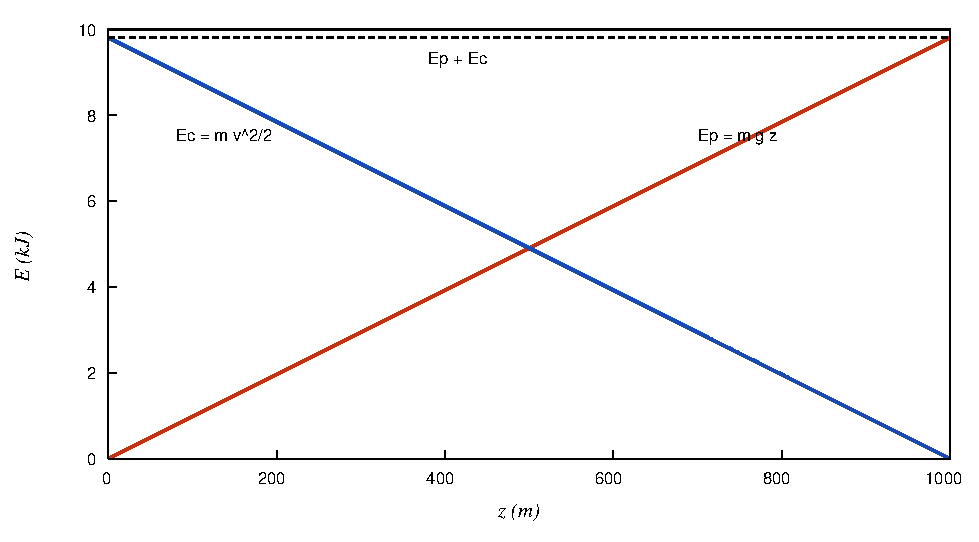
\includegraphics{../figures/FIG-0047/figure.pdf}}%
\count0=\ht0
\advance\count0 by \dp0
\count2=\wd0
\count4=\dimexpr\textheight/100*38\relax
\count6=\linewidth
\ifnum\count0<1
\count0=1
\fi
\ifnum\count2<1
\count2=1
\fi
\divide\count0 by 4096
\divide\count2 by 4096
\divide\count4 by 4096
\divide\count6 by 4096
\ifnum\count0<1
\count0=1
\fi
\ifnum\count2<1
\count2=1
\fi
\ifnum\count4<1
\count4=1
\fi
\ifnum\count6<1
\count6=1
\fi
\count8=\count2
\ifnum\count0>\count4
\count8=\numexpr\count2*\count4/\count0\relax
\fi
\ifnum\count8>\count6
\resizebox{\linewidth}{!}{\box0}%
\else
\ifnum\count0>\count4
\resizebox{!}{\dimexpr\textheight/100*38\relax}{\box0}%
\else
\box0%
\fi
\fi
\endgroup
\par\nopagebreak
\studiumcaption{fig:c01-energia}{Energía potencial \(m g z\), energía cinética \(\tfrac12 mv^{2}\) y energía mecánica total de una masa de 1 kg que cae sin rozamiento desde 1000 m de altura (\(g = 9.81\) m/s\(^2\)), en función de la altura \(z\): la suma permanece constante.}
\end{minipage}
\par\vspace{\baselineskip}

\par\vspace{\baselineskip}
\noindent\begin{minipage}{\linewidth}
\centering
\begingroup
\setbox0=\hbox{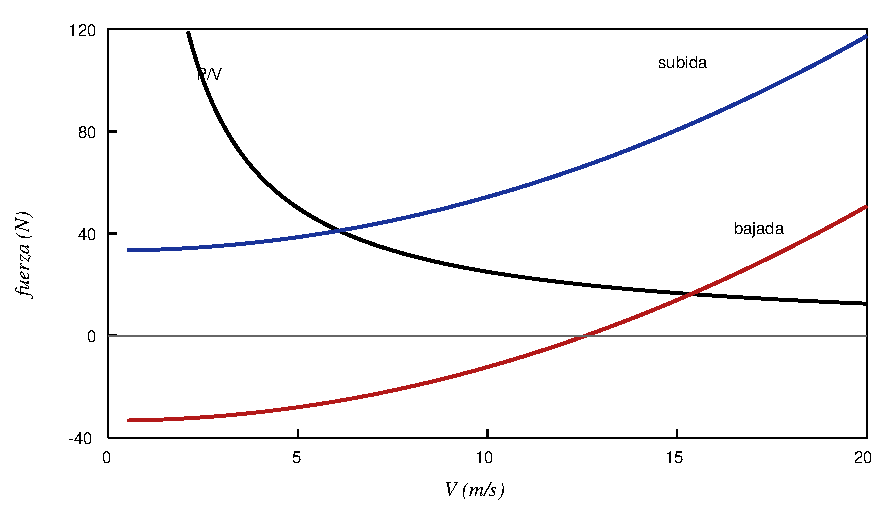
\includegraphics{../figures/FIG-0068/figure.pdf}}%
\count0=\ht0
\advance\count0 by \dp0
\count2=\wd0
\count4=\dimexpr\textheight/100*38\relax
\count6=\linewidth
\ifnum\count0<1
\count0=1
\fi
\ifnum\count2<1
\count2=1
\fi
\divide\count0 by 4096
\divide\count2 by 4096
\divide\count4 by 4096
\divide\count6 by 4096
\ifnum\count0<1
\count0=1
\fi
\ifnum\count2<1
\count2=1
\fi
\ifnum\count4<1
\count4=1
\fi
\ifnum\count6<1
\count6=1
\fi
\count8=\count2
\ifnum\count0>\count4
\count8=\numexpr\count2*\count4/\count0\relax
\fi
\ifnum\count8>\count6
\resizebox{\linewidth}{!}{\box0}%
\else
\ifnum\count0>\count4
\resizebox{!}{\dimexpr\textheight/100*38\relax}{\box0}%
\else
\box0%
\fi
\fi
\endgroup
\par\nopagebreak
\studiumcaption{fig:c01-resistencia}{Ciclista del ejemplo (\(M = 85\) kg, pendiente del 4 \%, \(C_D A = 0.35\) m\(^2\), \(P = 250\) W): fuerza motriz disponible \(P/V\) (negro) y resistencia total en subida, \(Mg\sin\varphi + k_D V^{2}\) (azul), y en bajada, \(k_D V^{2} - Mg\sin\varphi\) (rojo). Las intersecciones son las velocidades máximas, 6.08 y 15.37 m/s.}
\end{minipage}
\par\vspace{\baselineskip}

La segunda ley, en su forma moderna, establece que la derivada temporal del momento lineal de una partícula, \(\mathbf{p} = m\mathbf{v}\), es igual a la fuerza neta que actúa sobre ella:
\begin{equation}
\mathbf{F} = \frac{d\mathbf{p}}{dt}. \label{eq:c01-segunda}
\end{equation}
Cuando la masa es constante la ecuación se reduce a la forma familiar \(\mathbf{F} = m\mathbf{a}\). Es importante subrayar que la ecuación \(\eqref{eq:c01-segunda}\) se aplica a un conjunto fijo de partículas; escribir \(\mathbf{F} = m\,d\mathbf{v}/dt + \mathbf{v}\,dm/dt\) para un cuerpo que pierde masa, como un cohete, conduce a resultados incorrectos, porque el término \(\mathbf{v}\,dm/dt\) no tiene en cuenta la velocidad con la que la masa abandona el cuerpo. Esta observación es el germen del tratamiento de los volúmenes de control del capítulo 9, en el que el sistema de partículas sobre el que se aplica la segunda ley se distingue cuidadosamente de la región del espacio que se observa. La tercera ley completa el cuadro: si un cuerpo ejerce una fuerza sobre otro, este ejerce sobre el primero una fuerza de igual módulo y sentido opuesto. La paráfrasis «acción igual a reacción» induce a error si se olvida que acción y reacción actúan sobre cuerpos distintos, por lo que nunca se cancelan en el diagrama de sólido libre de un único cuerpo. Las tres leyes se emplean conjuntamente mediante un procedimiento que conviene automatizar: aislar el sistema, dibujar todas las fuerzas exteriores que actúan sobre él, elegir un sistema de referencia inercial y unos ejes, y solo entonces escribir la segunda ley componente a componente.

\section{Momento lineal y momento angular}

Integrando la ecuación \(\eqref{eq:c01-segunda}\) entre dos instantes se obtiene el teorema del impulso, \(\mathbf{p}_2 - \mathbf{p}_1 = \int_{t_1}^{t_2}\mathbf{F}\,dt\): la variación del momento lineal es igual al impulso de la fuerza neta. Esta forma es especialmente útil cuando las fuerzas son muy intensas y de corta duración, como en un impacto, porque permite estimar la fuerza media sin conocer su evolución detallada. Por ejemplo, un ave de \(1.8\) kg que golpea un parabrisas que avanza a 80 m/s y queda adherida a él en unos 2 ms recibe un impulso igual a su cambio de momento lineal, de modo que la fuerza media vale \(1.8\cdot 80/0.002 = 72\,000\) N; la cifra explica por qué la certificación de aeronaves exige ensayos específicos de impacto de aves. Cuando la fuerza neta sobre un sistema es nula, su momento lineal total se conserva, y lo hace simultáneamente en las tres direcciones del espacio. Para un sistema de dos o más cuerpos que solo interaccionan entre sí, la tercera ley garantiza que las fuerzas interiores no alteran el momento lineal total, aunque puedan redistribuirlo entre las partes: así se explica el retroceso de un astronauta que lanza una herramienta en ingravidez, o el de un arma al disparar.

El momento angular de una partícula respecto a un punto \(O\) se define como el momento de su momento lineal, \(\mathbf{L}_O = \mathbf{r}\times m\mathbf{v}\), donde \(\mathbf{r}\) es el vector de posición medido desde \(O\). A diferencia del momento lineal, el momento angular depende de la elección del origen, y por eso debe indicarse siempre el punto de referencia. Derivando con la regla del producto y teniendo en cuenta que \(\mathbf{v}\times m\mathbf{v} = \mathbf{0}\), se obtiene
\begin{equation}
\frac{d\mathbf{L}_O}{dt} = \mathbf{r}\times\mathbf{F} = \mathbf{M}_O, \label{eq:c01-momang}
\end{equation}
es decir, el momento resultante de las fuerzas respecto a un punto fijo es la tasa de variación del momento angular respecto a ese punto. Si el momento de las fuerzas exteriores es nulo, el momento angular se conserva. Una fuerza central, dirigida siempre hacia \(O\), produce momento nulo respecto a ese punto; por eso un satélite en órbita kepleriana barre áreas iguales en tiempos iguales. Para un sólido continuo o para un fluido, el momento angular total es la integral de volumen de la densidad de momento angular, y la ecuación \(\eqref{eq:c01-momang}\) reaparecerá en el capítulo 14 como la condición que obliga a que el tensor de esfuerzos sea simétrico.

\section{Sistemas de partículas y sólido rígido}

Consideremos ahora un sistema de \(N\) partículas de masas \(m_i\) y posiciones \(\mathbf{r}_i\), sometidas a fuerzas exteriores \(\mathbf{F}_i^{\mathrm{ext}}\) y a fuerzas de interacción mutua \(\mathbf{f}_{ij}\), ejercidas por la partícula \(j\) sobre la \(i\). La segunda ley aplicada a cada partícula da
\begin{equation}
m_i\,\ddot{\mathbf{r}}_i = \mathbf{F}_i^{\mathrm{ext}} + \sum_{j\neq i}\mathbf{f}_{ij}. \label{eq:c01-particula}
\end{equation}
Al sumar para todas las partículas, la doble suma de fuerzas interiores se anula por pares, porque \(\mathbf{f}_{ij} = -\mathbf{f}_{ji}\). Si se define la posición del centro de masas como \(\mathbf{R}_G = M^{-1}\sum_i m_i\mathbf{r}_i\), con \(M = \sum_i m_i\), el resultado es el teorema del centro de masas,
\begin{equation}
M\,\frac{d^{2}\mathbf{R}_G}{dt^{2}} = \sum_i \mathbf{F}_i^{\mathrm{ext}}, \label{eq:c01-tcm}
\end{equation}
que afirma que el centro de masas se mueve como una partícula de masa \(M\) sobre la que actuasen todas las fuerzas exteriores. El resultado es notable por lo que no exige: no hace falta que el sistema sea rígido ni conocer las fuerzas interiores. Por eso será aplicable sin cambios a una porción material de fluido, cuyas partículas se deforman y se mezclan, siempre que se siga a las mismas partículas. La figura~\ref{fig:c01-sistema} resume la notación.

Para el momento angular de un sistema el razonamiento es análogo, pero exige una hipótesis adicional: que las fuerzas interiores sean centrales, esto es, dirigidas según la recta que une cada par de partículas. Con esa condición sus momentos también se cancelan por pares y la derivada \(d\mathbf{L}_O/dt\) iguala al momento de las fuerzas exteriores, \(\mathbf{M}_O^{\mathrm{ext}}\), para un punto \(O\) fijo, o bien para el centro de masas aunque este se mueva. En un sólido rígido las distancias entre partículas son constantes y su movimiento queda descrito por la velocidad de un punto de referencia y por un único vector velocidad angular \(\boldsymbol{\Omega}\), de modo que la velocidad de cada punto es \(\mathbf{v}_i = \mathbf{v}_G + \boldsymbol{\Omega}\times(\mathbf{r}_i - \mathbf{R}_G)\). Cuando el sólido gira alrededor de un eje fijo, la componente del momento angular según ese eje vale \(L = I\Omega\), con \(I = \sum_i m_i d_i^{2}\) el momento de inercia respecto al eje y \(d_i\) la distancia de cada partícula a él; la ecuación del momento angular se reduce entonces a que \(I\,d\Omega/dt\) iguale al momento \(M_{\mathrm{eje}}\) de las fuerzas exteriores respecto al eje, el análogo rotacional de \(F = ma\). Para una varilla delgada y uniforme de masa \(m\) y longitud \(\ell\) que gira alrededor de uno de sus extremos, \(I = m\ell^{2}/3\), valor que se usará en los ejercicios para modelar la pala de un rotor. Los ejes principales de inercia y las ecuaciones de Euler del sólido rígido generalizan este resultado al caso tridimensional; su estudio detallado corresponde a la mecánica del vuelo.

\section{Trabajo, energía y fuerzas conservativas}

El trabajo de una fuerza a lo largo de una trayectoria \(C\) entre las posiciones 1 y 2 se define como la integral de línea \(W_{12} = \int_C \mathbf{F}\cdot d\mathbf{r}\). Si \(\mathbf{F}\) es la fuerza resultante sobre una partícula de masa constante, la segunda ley permite escribir \(\mathbf{F}\cdot d\mathbf{r} = m\,(d\mathbf{v}/dt)\cdot\mathbf{v}\,dt\), y como \(\mathbf{v}\cdot d\mathbf{v}/dt\) es la derivada temporal de \(v^{2}/2\), la integral se evalúa sin conocer la trayectoria:
\begin{equation}
W_{12} = \int_{1}^{2}\mathbf{F}\cdot d\mathbf{r} = \tfrac{1}{2}m v_2^{2} - \tfrac{1}{2}m v_1^{2}. \label{eq:c01-tte}
\end{equation}
Este es el teorema del trabajo y la energía cinética: el trabajo neto positivo aumenta la energía cinética, \(E_c = \tfrac12 m v^{2}\), y el negativo la disminuye. Su ventaja frente a la segunda ley es que es una ecuación escalar que relaciona directamente velocidades y desplazamientos, sin pasar por el tiempo. Su limitación es que, en un sistema deformable, las fuerzas interiores sí realizan trabajo aunque no alteren el momento lineal total; en un fluido, ese trabajo interior es el que la viscosidad transforma irreversiblemente en energía interna, y aparecerá en el capítulo 14 como función de disipación.

Una fuerza es conservativa cuando el trabajo que realiza entre dos puntos no depende del camino seguido; de forma equivalente, su circulación a lo largo de cualquier curva cerrada es nula, \(\oint_C \mathbf{F}\cdot d\mathbf{r} = 0\). En una región simplemente conexa estas condiciones equivalen a que el rotacional de la fuerza sea nulo y a que la fuerza derive de una energía potencial, \(\mathbf{F} = -\nabla E_p\). Una fuerza conservativa depende solo de la posición, de modo que su trabajo se escribe como \(W_{12} = -(E_{p,2} - E_{p,1})\); combinando este resultado con el teorema \(\eqref{eq:c01-tte}\) se obtiene la conservación de la energía mecánica, \(E_c + E_p = \text{cte}\), siempre que solo trabajen fuerzas conservativas. En un campo gravitatorio uniforme con el eje \(z\) vertical hacia arriba, \(E_p = m g z\) y
\begin{equation}
\tfrac{1}{2}m v_2^{2} + m g z_2 = \tfrac{1}{2}m v_1^{2} + m g z_1. \label{eq:c01-energia}
\end{equation}
Un cuerpo que cae 1000 m partiendo del reposo alcanzaría, sin resistencia del aire, una celeridad \(v = \sqrt{2\cdot 9.81\cdot 1000} \approx 140.1\) m/s; durante la caída la energía potencial se transforma en cinética sin que cambie su suma, como muestra la figura~\ref{fig:c01-energia}. La comparación con las velocidades terminales reales, mucho menores, muestra la importancia de la fuerza de resistencia, que no es conservativa y que se estudia en el capítulo 7. La ecuación \(\eqref{eq:c01-energia}\) es el antecedente directo de la ecuación de Bernoulli del capítulo 12, en la que la presión aporta un término de trabajo adicional.

Los conceptos anteriores se formulan de manera natural con campos. Un campo escalar asigna un número a cada punto del espacio y de cada instante, como la energía potencial gravitatoria por unidad de masa \(g z\), la temperatura o la presión; un campo vectorial asigna un vector, como la fuerza gravitatoria por unidad de masa o la velocidad del aire alrededor de un ala. La relación \(\mathbf{F} = -\nabla E_p\) es la primera aparición en este libro de un operador diferencial que transforma un campo escalar en uno vectorial: el gradiente apunta en la dirección de máximo crecimiento del campo y su módulo es la tasa de crecimiento en esa dirección. La condición de rotacional nulo para una fuerza conservativa tiene su réplica exacta en la mecánica de fluidos: un campo de velocidades irrotacional deriva de un potencial de velocidad, y gran parte de la aerodinámica clásica se apoya en esa propiedad. El paso de la mecánica de partículas a la de medios continuos consiste, precisamente, en sustituir sumas sobre partículas por integrales de volumen de densidades de masa, de momento lineal, de momento angular y de energía; los operadores gradiente, divergencia y rotacional, y los teoremas integrales que los relacionan, se desarrollan en el capítulo 11.

Muchos problemas de dinámica de vehículos no dan el modelo: describen una situación y piden un parámetro que hay que deducir. El método es siempre el mismo. Primero se elige el sistema (el vehículo como partícula de masa \(M\)) y unos ejes, aquí uno paralelo a la calzada, positivo en el sentido del movimiento, y otro normal a ella. Después se dibujan todas las fuerzas: el peso, cuya componente a lo largo de una pendiente de ángulo \(\varphi\) vale \(Mg\sin\varphi\) y frena en subida y empuja en bajada; la reacción normal de la calzada, que no trabaja; la fuerza de tracción \(F_t\) que la calzada ejerce sobre las ruedas motrices; y la resistencia aerodinámica, opuesta a la velocidad relativa al aire, que en régimen de número de Reynolds alto es cuadrática, \(D = \tfrac12\rho C_D A V^{2} = k_D V^{2}\) con \(k_D = \rho C_D A/2\). La segunda ley de Newton a lo largo de la calzada da, en subida,
\begin{equation}
M\,\frac{dV}{dt} = F_t - Mg\sin\varphi - k_D V^{2}. \label{eq:c01-pendiente}
\end{equation}
La expresión velocidad máxima constante contiene dos datos físicos: que la aceleración es nula, de modo que \(\eqref{eq:c01-pendiente}\) se convierte en un equilibrio algebraico, y que el motor trabaja en su límite. Qué significa ese límite es la decisión de modelado que determina la respuesta.

Supongamos que se conocen las velocidades máximas en subida, \(V_1\), y en bajada, \(V_2 > V_1\), por la misma carretera y sin viento, y que se busca \(k_D\). Hay dos incógnitas, \(k_D\) y el límite del motor, y dos condiciones de operación: el problema está determinado, y la técnica es eliminar la incógnita que no interesa. Con la hipótesis de fuerza de tracción máxima constante, \(F_t = Mg\sin\varphi + k_D V_1^{2}\) en subida y \(F_t + Mg\sin\varphi = k_D V_2^{2}\) en bajada; restando,
\begin{equation}
k_D = \frac{2Mg\sin\varphi}{V_2^{2} - V_1^{2}},\qquad F_t = Mg\sin\varphi + k_D V_1^{2}. \label{eq:c01-fuerza-constante}
\end{equation}
Con la hipótesis de potencia máxima constante, para velocidades de avance \(V>0\) la fuerza de tracción es \(P/V\), porque la potencia es el producto de la fuerza por la velocidad: \(\frac{P}{V_1} = Mg\sin\varphi + k_D V_1^{2}\) y \(\frac{P}{V_2} + Mg\sin\varphi = k_D V_2^{2}\). Igualando las dos expresiones de \(P\) se elimina la potencia:
\begin{equation}
k_D = \frac{Mg\sin\varphi\,(V_1 + V_2)}{V_2^{3} - V_1^{3}},\qquad P = V_1\left(Mg\sin\varphi + k_D V_1^{2}\right). \label{eq:c01-potencia-constante}
\end{equation}
Las dos fórmulas no son equivalentes. Con \(r = V_2/V_1 > 1\), el cociente entre las dos constantes es \(2\,(r^{2} + r + 1)/(r + 1)^{2}\), que tiende a \(\tfrac{3}{2}\) cuando \(r \to 1\), crece monótonamente con \(r\) (su derivada es \(2\,(r - 1)/(r + 1)^{3}\)) y tiende a 2 cuando \(r \to \infty\). Por tanto, el modelo de fuerza constante da siempre una constante de resistencia entre un 50 \% y un 100 \% mayor que el de potencia constante: los dos modelos no coinciden para ningún par de datos. El límite \(r \to 1\) no es un caso en que los modelos se reconcilien, sino uno en que el ensayo deja de servir: dos velocidades iguales solo se dan con pendiente nula, y entonces ambas fórmulas son indeterminadas, del tipo 0/0. Por eso un resultado sin la hipótesis explícita está incompleto. Si además el motor no actúa (descenso en punto muerto), la condición se reduce a \(Mg\sin\varphi = k_D V^{2}\), que es la velocidad terminal del capítulo 7 con la componente del peso en lugar del peso.

Ejemplo resuelto. Un ciclista de 85 kg (con la bicicleta) sube una pendiente del 4 \% (la tangente del ángulo vale 0.04) a una velocidad máxima de 6.08 m/s y la baja pedaleando a fondo a 15.37 m/s; el aire, en calma, tiene una densidad de 1.2 kg/m\(^3\), y se desprecia la resistencia a la rodadura. La componente del peso vale \(85\cdot 9.81\cdot\sin(\arctan 0.04) = 33.327\) N. Con la hipótesis de potencia constante, la más razonable para un ciclista, cuyo límite fisiológico es aproximadamente una potencia, \(\eqref{eq:c01-potencia-constante}\) da un área de resistencia \(C_D A\), igual a \(2k_D/\rho\), de 0.3498 m\(^2\) y una potencia de 249.8 W, valores típicos de un ciclista en posición erguida. Con la hipótesis de fuerza constante, los mismos datos darían un área de resistencia de 0.5575 m\(^2\), un 59 \% más, y una potencia distinta en subida y en bajada; es el cociente \(2\,(r^{2} + r + 1)/(r + 1)^{2}\) con \(r = 15.37/6.08\). Los datos no pueden decidir entre ambos modelos, porque los dos ajustan exactamente las dos velocidades; lo decide la física del motor. Comprobación dimensional: \(Mg\sin\varphi/V^{2}\) tiene unidades de kg/m, como \(k_D\), y \(V\,(Mg\sin\varphi + k_D V^{2})\) tiene unidades de W. La figura~\ref{fig:c01-resistencia} muestra el equilibrio gráfico entre la fuerza motriz disponible y la resistencia total en ambos sentidos de la marcha.

Fuera del régimen estacionario, \(\eqref{eq:c01-pendiente}\) es una ecuación diferencial no lineal. Con potencia constante, \(M\,dV/dt = P/V - Mg\sin\varphi - k_D V^{2}\), y, para una condición inicial con \(V(0)>0\), la velocidad tiende al único equilibrio positivo: la fuerza neta modelizada es estrictamente decreciente con \(V\), pues su derivada es \(-P/V^{2}-2k_DV<0\). La velocidad de equilibrio es estable. El modelo idealizado no está definido en \(V=0\) porque \(P/V\) diverge; por tanto, no describe por sí solo el arranque desde el reposo y debe completarse allí con una ley de tracción físicamente limitada. La práctica 2 integra esta ecuación numéricamente y mide cuánto tarda el vehículo en alcanzar ese régimen. Los mismos razonamientos se aplican a un avión en ascenso o descenso con empuje constante (turborreactor) o potencia constante (motor de hélice), a un esquiador o a un dron: lo que cambia es qué fuerza es constante y qué fuerzas mecánicas, como la rodadura o el rozamiento, acompañan a la resistencia aerodinámica.

\begin{tcolorbox}[title={Consejo}, studiumtip, breakable]

Antes de escribir cualquier ecuación de balance, diga explícitamente cuál es el sistema: qué partículas incluye y si su masa es constante. La mayoría de los errores con la tercera ley, con los cuerpos de masa variable y, más adelante, con los volúmenes de control proceden de cambiar de sistema a mitad del razonamiento sin advertirlo.

Antes de escribir una ecuación, enumere las incógnitas y las condiciones de operación: con dos regímenes medidos se pueden eliminar dos incógnitas, no más. Indique siempre qué es constante entre los regímenes (la fuerza, la potencia o nada) y por qué; y compruebe al final que el resultado tiene sentido físico, por ejemplo que el \(C_D\) obtenido está entre 0.2 y 1.2 para un vehículo terrestre.
\end{tcolorbox}

\begin{tcolorbox}[title={Definición}, studiumdef, breakable]

Sistema de referencia inercial: sistema de referencia en el que una partícula sobre la que no actúa ninguna fuerza neta permanece en reposo o en movimiento rectilíneo uniforme. Todos los sistemas inerciales se trasladan unos respecto a otros con velocidad constante y sin rotación relativa.
\end{tcolorbox}



\section{Desarrollos y práctica}

Las deducciones que siguen recogen, con sus hipótesis explícitas, los resultados en los que se apoya el resto del libro: el teorema del centro de masas \(\eqref{eq:c01-tcm}\), que permite tratar un sistema de partículas como una única masa sometida solo a las fuerzas exteriores; la ecuación del momento angular \(\eqref{eq:c01-momang}\), que reaparecerá en las turbomáquinas y en los fluidos en rotación; y el teorema del trabajo y la energía \(\eqref{eq:c01-tte}\), del que la conservación de la energía mecánica \(\eqref{eq:c01-energia}\) es el caso particular de fuerzas conservativas. El problema resuelto aplica estas leyes a un caso completo, y los ejercicios están ordenados de menor a mayor dificultad: los primeros se resuelven aplicando directamente una ecuación, mientras que los últimos exigen elegir el sistema, decidir qué fuerzas son exteriores y comprobar las hipótesis. Cuando el resultado numérico de un ejercicio dependa de un dato redondeado, conviene arrastrar todas las cifras hasta el final y redondear solo el resultado.

\begin{tcolorbox}[title={Desarrollos del modelo}, studiumdef, breakable]

\noindent\textbf{Teorema del centro de masas}

\[
M\,\frac{d^{2}\mathbf{R}_G}{dt^{2}} = \sum_i \mathbf{F}_i^{\mathrm{ext}}
\]

\noindent\textbf{Hipótesis}
\begin{itemize}
\item sistema cerrado de N partículas de masa constante
\item fuerzas interiores que cumplen la tercera ley en su forma débil (iguales y opuestas)
\item sistema de referencia inercial
\end{itemize}

\noindent\textbf{Limitaciones}
\begin{itemize}
\item no es válido directamente para sistemas de masa variable (cohetes): hay que aplicar la ley a un conjunto fijo de partículas
\end{itemize}

\noindent\textbf{Pasos}
\begin{enumerate}
\item
escribir la segunda ley para cada partícula separando fuerzas exteriores e interiores

\[
m_i\,\ddot{\mathbf{r}}_i = \mathbf{F}_i^{\mathrm{ext}} + \sum_{j\neq i}\mathbf{f}_{ij}
\]
\item
sumar para todas las partículas; las fuerzas interiores se anulan por pares

\[
\sum_i m_i\,\ddot{\mathbf{r}}_i = \sum_i \mathbf{F}_i^{\mathrm{ext}} + \sum_i\sum_{j\neq i}\mathbf{f}_{ij} = \sum_i \mathbf{F}_i^{\mathrm{ext}}
\]
\item
introducir la posición del centro de masas y derivar dos veces respecto al tiempo

\[
\mathbf{R}_G = \frac{1}{M}\sum_i m_i\,\mathbf{r}_i,\qquad M\,\ddot{\mathbf{R}}_G = \sum_i \mathbf{F}_i^{\mathrm{ext}}
\]
\end{enumerate}

\noindent\textbf{Variables}
\begin{itemize}
\item $M$: masa total ($\mathrm{kg}$)
\item $R_{G}$: posición del centro de masas ($\mathrm{m}$)
\item $F_{ext}$: fuerzas exteriores ($\mathrm{N}$)
\end{itemize}



\noindent\textbf{Ecuación del momento angular de una partícula}

\[
\frac{d\mathbf{L}_O}{dt} = \mathbf{r}\times\mathbf{F} = \mathbf{M}_O
\]

\noindent\textbf{Hipótesis}
\begin{itemize}
\item punto O fijo en un sistema de referencia inercial
\item masa constante
\end{itemize}

\noindent\textbf{Limitaciones}
\begin{itemize}
\item si el punto O se mueve aparece un término adicional proporcional a su velocidad
\item para un sistema se requiere que las fuerzas interiores sean centrales (forma fuerte de la tercera ley)
\end{itemize}

\noindent\textbf{Pasos}
\begin{enumerate}
\item
derivar el momento angular con la regla del producto

\[
\frac{d\mathbf{L}_O}{dt} = \frac{d\mathbf{r}}{dt}\times m\mathbf{v} + \mathbf{r}\times m\frac{d\mathbf{v}}{dt}
\]
\item
el producto vectorial de la velocidad por sí misma es nulo

\[
\mathbf{v}\times m\mathbf{v} = \mathbf{0}
\]
\item
sustituir la derivada del momento lineal por la fuerza resultante

\[
\frac{d\mathbf{L}_O}{dt} = \mathbf{r}\times\mathbf{F}
\]
\end{enumerate}

\noindent\textbf{Variables}
\begin{itemize}
\item $L_{O}$: momento angular respecto a O ($\mathrm{kg}\,\mathrm{m}^{2}\,\mathrm{s}^{-1}$)
\item $M_{O}$: momento de la fuerza respecto a O ($\mathrm{N}\,\mathrm{m}$)
\end{itemize}



\noindent\textbf{Teorema del trabajo y la energía cinética}

\[
W_{12} = \int_{1}^{2}\mathbf{F}\cdot d\mathbf{r} = \tfrac{1}{2}m v_2^{2} - \tfrac{1}{2}m v_1^{2}
\]

\noindent\textbf{Hipótesis}
\begin{itemize}
\item partícula de masa constante
\item sistema de referencia inercial
\end{itemize}

\noindent\textbf{Limitaciones}
\begin{itemize}
\item en un sistema deformable las fuerzas interiores también trabajan
\end{itemize}

\noindent\textbf{Pasos}
\begin{enumerate}
\item
multiplicar escalarmente la segunda ley por el desplazamiento elemental

\[
\mathbf{F}\cdot d\mathbf{r} = m\frac{d\mathbf{v}}{dt}\cdot\mathbf{v}\,dt
\]
\item
reconocer la derivada temporal de la energía cinética

\[
m\,\mathbf{v}\cdot\frac{d\mathbf{v}}{dt} = \frac{d}{dt}\left(\tfrac{1}{2}m v^{2}\right)
\]
\item
integrar entre las posiciones 1 y 2

\[
W_{12} = E_{c,2} - E_{c,1}
\]
\end{enumerate}

\noindent\textbf{Variables}
\begin{itemize}
\item $W_{12}$: trabajo de la fuerza resultante entre 1 y 2 ($\mathrm{J}$)
\item $v_{1}$: celeridad inicial ($\mathrm{m}\,\mathrm{s}^{-1}$)
\item $v_{2}$: celeridad final ($\mathrm{m}\,\mathrm{s}^{-1}$)
\end{itemize}



\noindent\textbf{Conservación de la energía mecánica en un campo gravitatorio uniforme}

\[
\tfrac{1}{2}m v_2^{2} + m g z_2 = \tfrac{1}{2}m v_1^{2} + m g z_1
\]

\noindent\textbf{Hipótesis}
\begin{itemize}
\item solo trabaja el peso (fuerza conservativa)
\item gravedad uniforme
\item eje z vertical hacia arriba
\end{itemize}

\noindent\textbf{Limitaciones}
\begin{itemize}
\item cualquier fuerza no conservativa (resistencia aerodinámica, rozamiento) rompe la conservación
\end{itemize}

\noindent\textbf{Pasos}
\begin{enumerate}
\item
el trabajo del peso entre 1 y 2 es menos la variación de energía potencial

\[
W_{12} = -\left(E_{p,2} - E_{p,1}\right) = -m g\,(z_2 - z_1)
\]
\item
igualar ese trabajo a la variación de energía cinética

\[
E_{c,2} + E_{p,2} = E_{c,1} + E_{p,1}
\]
\end{enumerate}

\noindent\textbf{Variables}
\begin{itemize}
\item $z$: cota sobre un nivel de referencia ($\mathrm{m}$)
\end{itemize}



\noindent\textbf{Resistencia cuadrática en subida y en bajada con fuerza de tracción constante}

\[
k_D = \frac{2Mg\sin\varphi}{V_2^{2} - V_1^{2}},\qquad F_t = Mg\sin\varphi + k_D V_1^{2}
\]

\noindent\textbf{Hipótesis}
\begin{itemize}
\item velocidades máximas constantes (aceleración nula)
\item la única fuerza disipativa es la resistencia aerodinámica \(k_D V^2\)
\item sin viento
\item la misma fuerza de tracción máxima en subida y en bajada
\end{itemize}

\noindent\textbf{Principios}
\begin{itemize}
\item segunda ley de Newton a lo largo de la pendiente
\end{itemize}

\noindent\textbf{Limitaciones}
\begin{itemize}
\item un motor real a plena carga no entrega una fuerza constante a cualquier velocidad
\end{itemize}

\noindent\textbf{Pasos}
\begin{enumerate}
\item
subida a V1

\[
F_t = Mg\sin\varphi + k_D V_1^{2}
\]
\item
bajada a V2 con la misma tracción

\[
F_t + Mg\sin\varphi = k_D V_2^{2}
\]
\item
restar para eliminar la tracción

\[
k_D\,(V_2^{2} - V_1^{2}) = 2Mg\sin\varphi
\]
\end{enumerate}

\noindent\textbf{Variables}
\begin{itemize}
\item $V_{1}$: velocidad máxima en subida ($\mathrm{m}\,\mathrm{s}^{-1}$)
\item $V_{2}$: velocidad máxima en bajada ($\mathrm{m}\,\mathrm{s}^{-1}$)
\item $M$: masa del vehículo ($\mathrm{kg}$)
\end{itemize}



\noindent\textbf{Resistencia cuadrática en subida y en bajada con potencia constante}

\[
k_D = \frac{Mg\sin\varphi\,(V_1 + V_2)}{V_2^{3} - V_1^{3}},\qquad P = V_1\left(Mg\sin\varphi + k_D V_1^{2}\right)
\]

\noindent\textbf{Hipótesis}
\begin{itemize}
\item velocidades máximas constantes
\item la potencia máxima \(P = F_t V\) es la misma en subida y en bajada
\item la única fuerza disipativa es la resistencia aerodinámica
\item sin viento
\end{itemize}

\noindent\textbf{Principios}
\begin{itemize}
\item segunda ley de Newton
\item potencia = fuerza por velocidad
\end{itemize}

\noindent\textbf{Limitaciones}
\begin{itemize}
\item supone rendimiento de transmisión constante y una marcha que permite usar la potencia máxima
\end{itemize}

\noindent\textbf{Pasos}
\begin{enumerate}
\item
subida: P/V1 = Mg sin(phi\() + k_D V1^2\)

\[
\frac{P}{V_1} = Mg\sin\varphi + k_D V_1^{2}
\]
\item
bajada: P/V2 + Mg sin(phi\() = k_D V2^2\)

\[
\frac{P}{V_2} + Mg\sin\varphi = k_D V_2^{2}
\]
\item
eliminar P igualando las dos expresiones de la potencia

\[
V_1\left(Mg\sin\varphi + k_D V_1^{2}\right) = V_2\left(k_D V_2^{2} - Mg\sin\varphi\right)
\]
\end{enumerate}

\noindent\textbf{Variables}
\begin{itemize}
\item $P$: potencia de tracción ($\mathrm{W}$)
\end{itemize}



\noindent\textbf{Cociente entre las constantes de los modelos de fuerza y de potencia constantes}

\begin{equation}
\frac{k_F}{k_P} = \frac{2\,(r^{2} + r + 1)}{(r + 1)^{2}},\qquad r = \frac{V_2}{V_1},\qquad \frac{3}{2} < \frac{k_F}{k_P} < 2\quad (r > 1)
\label{eq:c01-cociente-modelos}
\end{equation}

\noindent\textbf{Hipótesis}
\begin{itemize}
\item los mismos datos (V1, V2, M, pendiente) en ambos modelos
\item V2 > V1 > 0
\end{itemize}

\noindent\textbf{Principios}
\begin{itemize}
\item cociente de las dos expresiones de \(k_D\)
\end{itemize}

\noindent\textbf{Limitaciones}
\begin{itemize}
\item para r tendiendo a 1 ambas constantes son indeterminadas (pendiente nula)
\end{itemize}

\noindent\textbf{Pasos}
\begin{enumerate}
\item
dividir las dos constantes y simplificar con \(V2^3 - V1^3 = (V2 - V1)(V2^2 + V1 V2 + V1^2)\)

\[
\frac{k_F}{k_P} = \frac{2\,(V_2^{2} + V_1 V_2 + V_1^{2})}{(V_1 + V_2)^{2}}
\]
\item
escribir el cociente con r = V2/V1

\[
\frac{k_F}{k_P} = \frac{2\,(r^{2} + r + 1)}{(r + 1)^{2}}
\]
\item
límites y monotonía

\[
\frac{d}{dr}\,\frac{2\,(r^{2} + r + 1)}{(r + 1)^{2}} = \frac{2\,(r - 1)}{(r + 1)^{3}}
\]
\end{enumerate}

\noindent\textbf{Variables}
\begin{itemize}
\item $r$: cociente de velocidades V2/V1
\end{itemize}


\end{tcolorbox}

\begin{tcolorbox}[title={Problema resuelto}, studiumworked, breakable]

\noindent\textbf{Enunciado}
Un avión de transporte de \(70\,000\) kg inicia la carrera de despegue desde el reposo. Modele la fuerza neta horizontal (empuje menos resistencia aerodinámica y rozamiento de rodadura) como constante e igual a 150 kN. Calcule la aceleración, el tiempo necesario para alcanzar la velocidad de rotación de 75 m/s y la longitud de pista recorrida hasta ese instante. Compruebe el resultado con el teorema del trabajo y la energía.

\noindent\textbf{Datos}
\begin{itemize}
\item $m = 70000\,\mathrm{kg}$ — masa del avión
\item $F = 150000\,\mathrm{N}$ — fuerza neta horizontal media
\item $V = 75\,\mathrm{m}\,\mathrm{s}^{-1}$ — velocidad de rotación
\end{itemize}

\noindent\textbf{Incógnita}
longitud de la carrera de despegue s hasta alcanzar V

\noindent\textbf{Modelo físico}

\noindent\textit{Trabajo y energía con fuerza constante}

\[
s = \frac{m V^{2}}{2F}
\]

\noindent\textbf{Hipótesis}
\begin{itemize}
\item fuerza neta constante (en la realidad el empuje disminuye y la resistencia aumenta con la velocidad)
\item pista horizontal
\item avión tratado como partícula
\end{itemize}

\noindent\textbf{Desarrollo paso a paso}

\phantomsection\label{solution:mf-001}
\noindent\textbf{Elección del procedimiento.} Fijamos el eje positivo hacia delante, $t=0$ al iniciar la carrera, $v_0=0$ y $s_0=0$. La fuerza dada ya es neta: no se vuelve a restar resistencia. Como $m$ y $F$ son constantes, $F=ma$ da aceleración constante. Primero se obtiene $a$; después se integra $dv/dt=a$ y finalmente $ds/dt=v$.

\begin{enumerate}

\item De $F=ma$ dividimos por la masa. Esta aceleración, no una velocidad, determina cuánto aumenta $v$ cada segundo.

\[\fitmath{a=\frac{F}{m}}\]

\[\fitmath{a=\frac{(150000)}{(70000)}\approx 2.142857\,\mathrm{m/s^{2}}}\]

\item Integrar entre $0$ y $t$ da $V-v_0=at$. Como $v_0=0$, despejar el instante de rotación da $t=V/a$.

\[\fitmath{t=\frac{V}{a}}\]

\[\fitmath{t=\frac{(75)}{(2.142857143)}\approx 35\,\mathrm{s}}\]

\item La velocidad crece desde cero; por ello no se usa $Vt$. La integral $s=\int_0^t a\xi\,d\xi$ da $at^2/2$.

\[\fitmath{s=\frac{a\cdot {t}^{2}}{2}}\]

\[\fitmath{s=\frac{(2.142857143)\cdot {(35)}^{2}}{2}\approx 1312.5\,\mathrm{m}}\]

\item Contraste de trabajo: una fuerza constante y paralela al desplazamiento realiza $W=Fs$.

\[\fitmath{W=F\cdot s}\]

\[\fitmath{W=(150000)\cdot (1312.5)\approx 1.96875\times10^{8}\,\mathrm{J}}\]

\item La energía cinética inicial es cero. El mismo trabajo debe coincidir con $mV^2/2$.

\[\fitmath{E=\frac{m\cdot {V}^{2}}{2}}\]

\[\fitmath{E=\frac{(70000)\cdot {(75)}^{2}}{2}\approx 1.96875\times10^{8}\,\mathrm{J}}\]

\end{enumerate}

\noindent\textbf{Contraste y comparación.} Las dos energías coinciden: $Fs=196\,875\,000\,\mathrm{J}$. Además, la velocidad media es $(0+75)/2=37.5\,\mathrm{m/s}$ y $s=37.5(35)=1312.5\,\mathrm m$. También es válida la ruta directa $s=mV^2/(2F)$ para hallar la distancia. Si tu resultado es $2625$ m, probablemente usaste la velocidad final durante toda la carrera; si difiere por mil, revisa kN frente a N.


\noindent\textbf{Sustitución numérica}

\[
\frac{\left(\left(75\,\mathrm{m}\,\mathrm{s}^{-1}\right)\right)^{2} \left(70000\,\mathrm{kg}\right)}{2 \left(150000\,\mathrm{N}\right)}
\]

\noindent\textbf{Resultado}\quad\(a=\frac{15}{7}\,\mathrm{m/s^2},\quad t=35\,\mathrm{s},\quad s=1312.5\,\mathrm{m}.\)

\noindent\textbf{Interpretación}
En el modelo dado, la distancia hasta la velocidad de rotación es 1312.5 m. No representa una distancia certificada de despegue: faltan la variación de fuerzas, la rotación y el ascenso posterior.

\noindent\textbf{Comprobación de la respuesta} la aritmética del último paso reproduce la respuesta enunciada a la precisión con que está escrita. Es una reproducción aritmética; no valida el modelo físico ni sus hipótesis.

\noindent\textbf{Limitaciones}
\begin{itemize}
\item el modelo de fuerza constante ignora la variación real de la fuerza neta con la velocidad
\item no incluye la fase de rotación ni el ascenso posterior
\end{itemize}

\noindent\textbf{Errores frecuentes}
\begin{itemize}
\item usar el empuje bruto en lugar de la fuerza neta
\item confundir la velocidad de rotación con la de despegue
\end{itemize}
\end{tcolorbox}

\begin{tcolorbox}[title={Ejercicios propuestos}, studiumworked, breakable]

\noindent\textbf{1 (Básico, Cálculo)}
Un astronauta de 80 kg (incluido el traje), inicialmente en reposo respecto a la estación espacial, lanza una herramienta de 20 kg que, inmediatamente después de separarse, tiene una velocidad de \(1.5\) m/s \emph{respecto a la estación espacial} (marco inercial aproximado). ¿Con qué celeridad retrocede el astronauta respecto a la estación?

\noindent\textbf{2 (Intermedio, Aplicación)}
Un satélite gira libremente alrededor de su eje de simetría a \(2.0\) rad/s con un momento de inercia de 1200 kg m\(^2\). Al desplegar unas antenas simétricas, el momento de inercia respecto a ese eje pasa a 1800 kg m\(^2\). Despreciando momentos exteriores, calcule la nueva velocidad angular.

\noindent\textbf{3 (Intermedio, Desarrollo)}
Un planeador de 400 kg desciende desde 1500 m hasta 900 m de altitud. Su celeridad inicial es 25 m/s y el trabajo de la resistencia aerodinámica durante el descenso es \(-1.5\) MJ. Tome \(g = 9.81\) m/s\(^2\) y calcule la celeridad final.

\noindent\textbf{4 (Avanzado, Aplicación)}
Un ave de \(1.8\) kg impacta contra el parabrisas de un avión que vuela a 80 m/s y queda adherida a él. Si la duración del impacto es de \(2.0\) ms, estime la fuerza media que el ave ejerce sobre el parabrisas. Desprecie la velocidad del ave antes del impacto.

\noindent\textbf{5 (De examen, Desarrollo)}
El rotor principal de un helicóptero tiene cuatro palas que pueden modelarse como varillas delgadas uniformes de 90 kg y \(7.0\) m de longitud articuladas en el eje. Partiendo del reposo, el motor aplica un par constante de 12 kN m. Despreciando la resistencia aerodinámica de las palas y la inercia del buje, calcule el tiempo necesario para alcanzar 30 rad/s.

\noindent\textbf{6 (Básico, Aplicación)}
Un ciclista de 90 kg (con la bicicleta) desciende sin pedalear una pendiente del 6 \% y alcanza una velocidad constante de 15.0 m/s en aire en calma (\(\rho = 1.2\) kg/m\(^3\)). Despreciando la rodadura, determine su área de resistencia \(C_D A\).

\noindent\textbf{7 (Avanzado, Desarrollo)}
En un circuito de pruebas con una pendiente del 3 \%, un coche eléctrico de 1600 kg y área frontal 2.3 m\(^2\) alcanza a plena potencia una velocidad máxima de 32.8 m/s en subida y de 50.7 m/s en bajada, sin viento (\(\rho = 1.2\) kg/m\(^3\)). Suponiendo que la potencia máxima de tracción es la misma en ambos sentidos y que la resistencia aerodinámica es la única fuerza disipativa, determine el coeficiente de resistencia y la potencia de tracción.

\noindent\textbf{8 (De examen, COMPARATIVE)}
Con los datos del ejercicio anterior (coche de 1600 kg, área frontal 2.3 m\(^2\), pendiente del 3 \%, 32.8 m/s en subida y 50.7 m/s en bajada, \(\rho = 1.2\) kg/m\(^3\)), un compañero resuelve el problema suponiendo que la fuerza de tracción máxima es la misma en subida y en bajada. (a) Plantee las ecuaciones con esa hipótesis y obtenga el \(C_D\) que resultaría. (b) Calcule con ese modelo la potencia que el motor tendría que entregar en subida y en bajada. (c) Sabiendo que el fabricante declara una potencia máxima de 30 kW, decida qué hipótesis es coherente y explique por qué los datos de velocidad por sí solos no pueden decidirlo.
\end{tcolorbox}

\begin{tcolorbox}[title={Autoevaluación}, studiumcheck, breakable]

(1) ¿Por qué no puede usarse \(\mathbf{F} = m\,d\mathbf{v}/dt + \mathbf{v}\,dm/dt\) para un cohete? (2) Si el momento de las fuerzas exteriores respecto al centro de masas de un satélite es nulo, ¿qué magnitud se conserva y qué ocurre con la velocidad de giro al desplegar unos paneles? (3) Demuestre que el trabajo del peso entre dos puntos solo depende de la diferencia de cotas. (4) ¿Qué hipótesis sobre las fuerzas interiores se necesita para el teorema del momento angular de un sistema que no hace falta para el del momento lineal? (5) Explique por qué el ensayo de un modelo fijo en un túnel con aire en movimiento es equivalente al vuelo del modelo en aire en reposo.

(1) Dibuje el diagrama de fuerzas de un vehículo que baja una pendiente con el motor a plena carga. (2) ¿Qué condición matemática expresa la frase velocidad máxima constante? (3) Deduzca \(k_D\) con la hipótesis de potencia constante eliminando \(P\). (4) Demuestre que el cociente entre las constantes de resistencia de los modelos de fuerza constante y de potencia constante está entre \(\tfrac{3}{2}\) y 2, y explique por qué un ensayo con \(V_1\) muy próxima a \(V_2\) no permite determinar \(k_D\). (5) ¿Qué hipótesis elegiría para un coche eléctrico limitado por la potencia de su motor, y cuál para un vehículo cuyas ruedas patinan? (6) ¿Qué cambia si sopla un viento de cara de velocidad \(w\)?
\end{tcolorbox}
\studiumchaptercheck

\chapter{Referencias no inerciales, mecánica lagrangiana y caos}
\label{chap:c02}

\studiumchapterguide{Este capítulo completa el Tema 1 con tres ideas que reaparecerán en el estudio de los fluidos. La primera es la descripción del movimiento desde sistemas de referencia no inerciales, imprescindible para entender la atmósfera terrestre, las turbomáquinas y los ensayos en centrifugadora. La segunda es la mecánica lagrangiana, que sustituye la contabilidad de fuerzas por una función escalar y permite tratar con elegancia sistemas con ligaduras. La tercera es el caos determinista: sistemas de ecuaciones sencillas y perfectamente deterministas cuya evolución es, en la práctica, impredecible a largo plazo, una propiedad que está en la raíz de la turbulencia y de los límites de la predicción meteorológica.}

\section{Sistemas de referencia no inerciales y fuerzas ficticias}

Las leyes de Newton se formulan en sistemas inerciales, pero muchas veces resulta más natural describir el movimiento desde un sistema que acelera: la cabina de un avión que despega, el rotor de un compresor o la superficie de la Tierra. Si el origen de un sistema de referencia se traslada sin girar con aceleración \(\mathbf{a}_0\) respecto a un sistema inercial, la aceleración de una partícula medida en el sistema móvil es \(\mathbf{a}' = \mathbf{a} - \mathbf{a}_0\), y la segunda ley adopta la forma \(m\mathbf{a}' = \mathbf{F} - m\mathbf{a}_0\). El término \(-m\mathbf{a}_0\) no procede de ninguna interacción física: es una fuerza de inercia, o pseudofuerza, que el observador acelerado debe añadir a las fuerzas reales para que la segunda ley siga siendo aplicable en su sistema. Un pasajero en un avión que acelera en pista se siente empujado contra el respaldo exactamente por esa razón; en el sistema de la pista, que es aproximadamente inercial, lo que ocurre es que el respaldo empuja al pasajero hacia delante. Las fuerzas de inercia más importantes en la práctica aparecen cuando el sistema de referencia gira: la fuerza centrífuga, que parece empujar los cuerpos hacia fuera del eje de giro, la fuerza de Coriolis, que actúa sobre los cuerpos que se mueven respecto al sistema giratorio, y la fuerza de Euler, que aparece cuando la velocidad angular del sistema varía.

\par\vspace{\baselineskip}
\noindent\begin{minipage}{\linewidth}
\centering
\begingroup
\setbox0=\hbox{\begin{tikzpicture}
\draw[->,thick] (0,0) -- (0,3.6) node[above]{$z$};
\draw[->,very thick,blue] (0,0.4) -- (0,1.6) node[left]{$\mathbf{\Omega}$};
\draw[->] (-0.35,2.6) arc (200:520:0.35 and 0.12);
\draw[dashed] (0,2.0) -- (3.0,2.0);
\fill (3.0,2.0) circle (2.4pt) node[above right]{$m$};
\draw[<->] (0,1.75) -- node[below]{$\rho$} (3.0,1.75);
\draw[->,very thick,red] (3.0,2.0) -- (4.3,2.0) node[right]{$-m\mathbf{\Omega}\times(\mathbf{\Omega}\times\mathbf{r}')$};
\draw[->,very thick] (3.0,2.0) -- (3.0,3.2) node[above]{$\mathbf{v}'$};
\draw[->,very thick,teal] (3.0,2.0) -- (2.1,2.9) node[above left]{$-2m\mathbf{\Omega}\times\mathbf{v}'$};
\draw[->,thick] (0,0) -- (2.95,1.95) node[midway,below right]{$\mathbf{r}'$};
\end{tikzpicture}}%
\count0=\ht0
\advance\count0 by \dp0
\count2=\wd0
\count4=\dimexpr\textheight/100*38\relax
\count6=\linewidth
\ifnum\count0<1
\count0=1
\fi
\ifnum\count2<1
\count2=1
\fi
\divide\count0 by 4096
\divide\count2 by 4096
\divide\count4 by 4096
\divide\count6 by 4096
\ifnum\count0<1
\count0=1
\fi
\ifnum\count2<1
\count2=1
\fi
\ifnum\count4<1
\count4=1
\fi
\ifnum\count6<1
\count6=1
\fi
\count8=\count2
\ifnum\count0>\count4
\count8=\numexpr\count2*\count4/\count0\relax
\fi
\ifnum\count8>\count6
\resizebox{\linewidth}{!}{\begin{tikzpicture}
\draw[->,thick] (0,0) -- (0,3.6) node[above]{$z$};
\draw[->,very thick,blue] (0,0.4) -- (0,1.6) node[left]{$\mathbf{\Omega}$};
\draw[->] (-0.35,2.6) arc (200:520:0.35 and 0.12);
\draw[dashed] (0,2.0) -- (3.0,2.0);
\fill (3.0,2.0) circle (2.4pt) node[above right]{$m$};
\draw[<->] (0,1.75) -- node[below]{$\rho$} (3.0,1.75);
\draw[->,very thick,red] (3.0,2.0) -- (4.3,2.0) node[right]{$-m\mathbf{\Omega}\times(\mathbf{\Omega}\times\mathbf{r}')$};
\draw[->,very thick] (3.0,2.0) -- (3.0,3.2) node[above]{$\mathbf{v}'$};
\draw[->,very thick,teal] (3.0,2.0) -- (2.1,2.9) node[above left]{$-2m\mathbf{\Omega}\times\mathbf{v}'$};
\draw[->,thick] (0,0) -- (2.95,1.95) node[midway,below right]{$\mathbf{r}'$};
\end{tikzpicture}}%
\else
\ifnum\count0>\count4
\resizebox{!}{\dimexpr\textheight/100*38\relax}{\begin{tikzpicture}
\draw[->,thick] (0,0) -- (0,3.6) node[above]{$z$};
\draw[->,very thick,blue] (0,0.4) -- (0,1.6) node[left]{$\mathbf{\Omega}$};
\draw[->] (-0.35,2.6) arc (200:520:0.35 and 0.12);
\draw[dashed] (0,2.0) -- (3.0,2.0);
\fill (3.0,2.0) circle (2.4pt) node[above right]{$m$};
\draw[<->] (0,1.75) -- node[below]{$\rho$} (3.0,1.75);
\draw[->,very thick,red] (3.0,2.0) -- (4.3,2.0) node[right]{$-m\mathbf{\Omega}\times(\mathbf{\Omega}\times\mathbf{r}')$};
\draw[->,very thick] (3.0,2.0) -- (3.0,3.2) node[above]{$\mathbf{v}'$};
\draw[->,very thick,teal] (3.0,2.0) -- (2.1,2.9) node[above left]{$-2m\mathbf{\Omega}\times\mathbf{v}'$};
\draw[->,thick] (0,0) -- (2.95,1.95) node[midway,below right]{$\mathbf{r}'$};
\end{tikzpicture}}%
\else
\begin{tikzpicture}
\draw[->,thick] (0,0) -- (0,3.6) node[above]{$z$};
\draw[->,very thick,blue] (0,0.4) -- (0,1.6) node[left]{$\mathbf{\Omega}$};
\draw[->] (-0.35,2.6) arc (200:520:0.35 and 0.12);
\draw[dashed] (0,2.0) -- (3.0,2.0);
\fill (3.0,2.0) circle (2.4pt) node[above right]{$m$};
\draw[<->] (0,1.75) -- node[below]{$\rho$} (3.0,1.75);
\draw[->,very thick,red] (3.0,2.0) -- (4.3,2.0) node[right]{$-m\mathbf{\Omega}\times(\mathbf{\Omega}\times\mathbf{r}')$};
\draw[->,very thick] (3.0,2.0) -- (3.0,3.2) node[above]{$\mathbf{v}'$};
\draw[->,very thick,teal] (3.0,2.0) -- (2.1,2.9) node[above left]{$-2m\mathbf{\Omega}\times\mathbf{v}'$};
\draw[->,thick] (0,0) -- (2.95,1.95) node[midway,below right]{$\mathbf{r}'$};
\end{tikzpicture}%
\fi
\fi
\endgroup
\par\nopagebreak
\studiumcaption{fig:c02-giratorio}{Sistema de referencia que gira con velocidad angular \(\mathbf{\Omega}\) alrededor del eje \(z\). Una partícula con velocidad relativa \(\mathbf{v}'\) experimenta, vista desde el sistema giratorio, la fuerza centrífuga, perpendicular al eje y hacia fuera, y la de Coriolis, perpendicular a \(\mathbf{v}'\) y a \(\mathbf{\Omega}\).}
\end{minipage}
\par\vspace{\baselineskip}

\par\vspace{\baselineskip}
\noindent\begin{minipage}{\linewidth}
\centering
\begingroup
\setbox0=\hbox{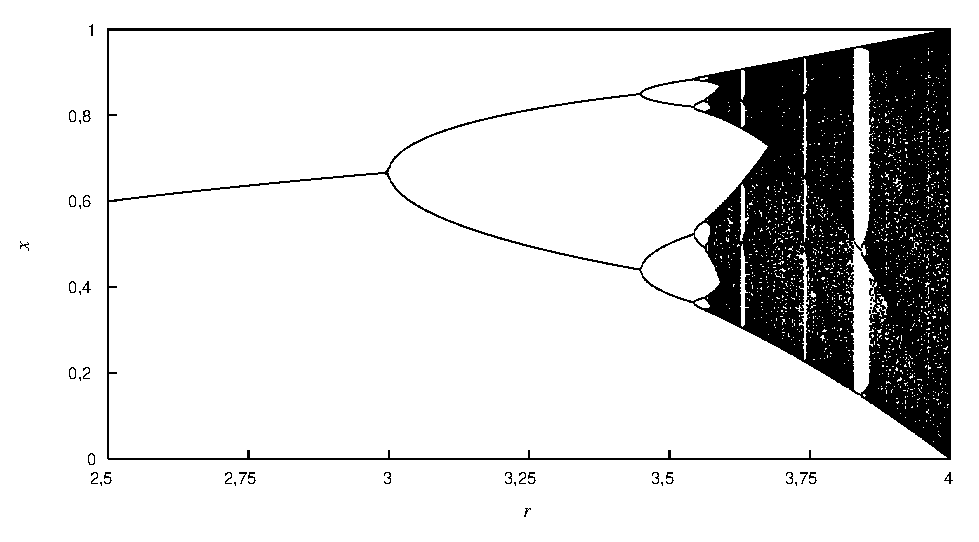
\includegraphics{../figures/FIG-0048/figure.pdf}}%
\count0=\ht0
\advance\count0 by \dp0
\count2=\wd0
\count4=\dimexpr\textheight/100*38\relax
\count6=\linewidth
\ifnum\count0<1
\count0=1
\fi
\ifnum\count2<1
\count2=1
\fi
\divide\count0 by 4096
\divide\count2 by 4096
\divide\count4 by 4096
\divide\count6 by 4096
\ifnum\count0<1
\count0=1
\fi
\ifnum\count2<1
\count2=1
\fi
\ifnum\count4<1
\count4=1
\fi
\ifnum\count6<1
\count6=1
\fi
\count8=\count2
\ifnum\count0>\count4
\count8=\numexpr\count2*\count4/\count0\relax
\fi
\ifnum\count8>\count6
\resizebox{\linewidth}{!}{\box0}%
\else
\ifnum\count0>\count4
\resizebox{!}{\dimexpr\textheight/100*38\relax}{\box0}%
\else
\box0%
\fi
\fi
\endgroup
\par\nopagebreak
\studiumcaption{fig:c02-bifurcacion}{Diagrama de bifurcación del mapa logístico \(x_{n+1} = r x_n (1 - x_n)\): para cada valor de \(r\) se representan los iterados 501 a 800 partiendo de \(x_0 = 0.2\). Se aprecian la cascada de duplicaciones de periodo y el régimen caótico a partir de \(r \approx 3.57\).}
\end{minipage}
\par\vspace{\baselineskip}

Para obtenerlas consideremos un sistema que gira con velocidad angular \(\boldsymbol{\Omega}\) respecto a un sistema inercial con el que comparte origen. La derivada temporal de cualquier vector \(\mathbf{b}\) vista desde el sistema inercial es la vista desde el sistema giratorio más un término debido al arrastre de los ejes,
\begin{equation}
\left(\frac{d\mathbf{b}}{dt}\right)_{\mathrm{in}} = \left(\frac{d\mathbf{b}}{dt}\right)_{\mathrm{rot}} + \boldsymbol{\Omega}\times\mathbf{b}. \label{eq:c02-regla}
\end{equation}
Aplicando la regla primero al vector de posición se obtiene \(\mathbf{v} = \mathbf{v}' + \boldsymbol{\Omega}\times\mathbf{r}'\), y aplicándola de nuevo a este resultado,
\begin{equation}
\mathbf{a} = \mathbf{a}' + 2\boldsymbol{\Omega}\times\mathbf{v}' + \boldsymbol{\Omega}\times\left(\boldsymbol{\Omega}\times\mathbf{r}'\right) + \dot{\boldsymbol{\Omega}}\times\mathbf{r}'. \label{eq:c02-acel}
\end{equation}
Despejando \(m\mathbf{a}'\) en la segunda ley aparecen, por este orden, la fuerza de Coriolis \(-2m\boldsymbol{\Omega}\times\mathbf{v}'\), la fuerza centrífuga \(-m\boldsymbol{\Omega}\times(\boldsymbol{\Omega}\times\mathbf{r}')\) y la fuerza de Euler \(-m\dot{\boldsymbol{\Omega}}\times\mathbf{r}'\). La fuerza centrífuga es perpendicular al eje de giro, está dirigida hacia fuera y tiene módulo \(m\Omega^{2}\rho\), siendo \(\rho\) la distancia al eje; es conservativa y deriva de la energía potencial \(-\tfrac12 m\Omega^{2}\rho^{2}\), por lo que suele agruparse con la gravedad en una gravedad efectiva. La fuerza de Coriolis es perpendicular a la velocidad relativa y, por tanto, no realiza trabajo: no cambia la celeridad relativa, solo la dirección del movimiento. La figura~\ref{fig:c02-giratorio} muestra la geometría de ambos términos. Conviene comprobar el resultado en un caso concreto: una partícula que se aleja radialmente con celeridad constante \(u\) a lo largo de un eje que gira con \(\Omega\) constante tiene, vista desde el sistema inercial, una componente de aceleración perpendicular al eje igual a \(2\Omega u\), que es precisamente el término de Coriolis; esa comprobación se ha realizado simbólicamente derivando dos veces la trayectoria inercial.

La Tierra gira con \(\Omega \approx 7.292\times 10^{-5}\) rad/s, una vuelta por día sidéreo. En el ecuador, la aceleración centrífuga vale \(\Omega^{2}R = (7.292\times 10^{-5})^{2}\cdot 6.371\times 10^{6} \approx 0.0339\) m/s\(^2\), alrededor del 0.35 \% de la gravedad; se incorpora a la gravedad efectiva y explica el ligero achatamiento del planeta. La fuerza de Coriolis tiene más consecuencias para los fluidos. Para movimientos horizontales, lo relevante es la componente vertical de la rotación, \(\Omega\sin\varphi\) en la latitud \(\varphi\), y la aceleración de Coriolis horizontal vale \(f\,v\), con el parámetro de Coriolis \(f = 2\Omega\sin\varphi\). En León, a unos \(42.6^\circ\) de latitud norte, \(f = 2\cdot 7.292\times 10^{-5}\sin(42.6^\circ) \approx 9.87\times 10^{-5}\) s\(^{-1}\). La desviación es hacia la derecha del movimiento en el hemisferio norte y hacia la izquierda en el sur, máxima en los polos y nula en el ecuador. Para un avión que vuela a 250 m/s la aceleración de Coriolis no supera \(2\cdot 7.292\times 10^{-5}\cdot 250 \approx 0.0365\) m/s\(^2\), despreciable frente a las aceleraciones de maniobra; en cambio, para una masa de aire que se mueve a 10 m/s durante días, el efecto acumulado domina la dinámica y conduce al equilibrio geostrófico del capítulo 16. La comparación se cuantifica con el número de Rossby, cociente entre la aceleración del movimiento y la de Coriolis, que se introduce allí.

\section{Mecánica lagrangiana}

La formulación de Newton exige identificar todas las fuerzas, incluidas las de ligadura, que en muchos problemas son desconocidas y carecen de interés: la tensión de la varilla de un péndulo o la reacción de una guía. La mecánica lagrangiana evita ese trabajo. Se eligen unas coordenadas generalizadas \(q_j\), tantas como grados de libertad tenga el sistema y compatibles con las ligaduras, y se construye la lagrangiana \(\mathcal{L}(q_j, \dot q_j, t) \equiv T - V\), diferencia entre la energía cinética y la potencial. El principio de acción estacionaria establece que, entre todas las evoluciones posibles entre dos configuraciones dadas, la real hace estacionaria la acción \(S = \int \mathcal{L}\,dt\). El cálculo de variaciones transforma esa condición en un sistema de ecuaciones diferenciales, las ecuaciones de Euler-Lagrange,
\begin{equation}
\frac{d}{dt}\left(\frac{\partial \mathcal{L}}{\partial \dot q_j}\right) - \frac{\partial \mathcal{L}}{\partial q_j} = 0, \qquad j = 1,\ldots,n. \label{eq:c02-el}
\end{equation}
Para un sistema con ligaduras ideales, que no realizan trabajo en los desplazamientos virtuales compatibles, estas ecuaciones son equivalentes a las de Newton, pero solo contienen las fuerzas activas a través de la energía potencial. Además revelan las cantidades conservadas de forma automática: si una coordenada \(q_k\) no aparece en \(\mathcal{L}\), su momento generalizado \(\partial\mathcal{L}/\partial\dot q_k\) se conserva, y si \(\mathcal{L}\) no depende explícitamente del tiempo se conserva la energía.

El péndulo simple ilustra el procedimiento. Con el ángulo \(\theta\) respecto a la vertical como única coordenada generalizada, una masa \(m\) en el extremo de una varilla rígida y sin masa de longitud \(\ell\) tiene \(T = \tfrac12 m\ell^{2}\dot\theta^{2}\) y \(V = -mg\ell\cos\theta\), de modo que \(\mathcal{L} = \tfrac12 m\ell^{2}\dot\theta^{2} + mg\ell\cos\theta\). Las derivadas parciales son \(\partial\mathcal{L}/\partial\dot\theta = m\ell^{2}\dot\theta\) y \(\partial\mathcal{L}/\partial\theta = -mg\ell\sin\theta\), y la ecuación \(\eqref{eq:c02-el}\) da
\begin{equation}
\ddot\theta + \frac{g}{\ell}\sin\theta = 0, \label{eq:c02-pendulo}
\end{equation}
sin haber tenido que calcular la tensión de la varilla. Para oscilaciones pequeñas, \(\sin\theta \approx \theta\) y la ecuación se reduce a la de un oscilador armónico de pulsación \(\omega_0 = \sqrt{g/\ell}\) y periodo \(2\pi\sqrt{\ell/g}\); un péndulo de un metro tiene un periodo \(2\pi\sqrt{1.0/9.81} \approx 2.006\) s. Este modelo de oscilador reaparece en el capítulo 8 aplicado a columnas de líquido y a cuerpos flotantes. Una advertencia terminológica es necesaria: en mecánica de fluidos, el adjetivo lagrangiano designa también la descripción del flujo que sigue a cada partícula de fluido, frente a la descripción euleriana que observa puntos fijos del espacio. Ambos usos rinden homenaje a Lagrange, pero son conceptos distintos; el segundo se estudia en el capítulo 4.

\section{Introducción a los sistemas caóticos}

Durante mucho tiempo se asumió que un sistema determinista, cuyas ecuaciones y condiciones iniciales se conocen, tiene una evolución predecible. El caos determinista muestra que no es así cuando el sistema es no lineal. El ejemplo más sencillo es el mapa logístico, una ecuación en diferencias de segundo grado,
\begin{equation}
x_{n+1} = r\,x_n\,(1 - x_n), \qquad 0 \le x_n \le 1,\quad 0 < r \le 4. \label{eq:c02-logistico}
\end{equation}
Sus puntos fijos se obtienen imponiendo \(x = r x(1-x)\): además de \(x = 0\) existe \(x^{*} = 1 - 1/r\), que es estable si el módulo de la derivada del mapa en él, \(|r(1-2x^{*})| = |2 - r|\), es menor que la unidad, es decir, para \(1\,< r < 3\). Al superar \(r = 3\) el punto fijo se desestabiliza y la sucesión pasa a oscilar entre dos valores; al seguir aumentando \(r\), la órbita de periodo 2 se desdobla en una de periodo 4, esta en una de periodo 8, y la cascada de duplicaciones de periodo se acumula en torno a \(r \approx 3.57\), más allá del cual aparece un comportamiento aperiódico con ventanas periódicas intercaladas. La figura~\ref{fig:c02-bifurcacion} muestra este diagrama de bifurcación, obtenido iterando numéricamente la ecuación \(\eqref{eq:c02-logistico}\). En el régimen caótico, dos condiciones iniciales que difieren en \(10^{-10}\) producen sucesiones que, tras unas pocas decenas de iteraciones, no guardan relación alguna: la incertidumbre crece exponencialmente.

El sistema de Lorenz traslada esas ideas a ecuaciones diferenciales con origen directamente fluidodinámico. Lorenz lo obtuvo como modelo extremadamente truncado de la convección en una capa de fluido calentada por debajo:
\begin{equation}
\dot x = \sigma\,(y - x),\qquad \dot y = x\,(\rho_R - z) - y,\qquad \dot z = x\,y - \beta z, \label{eq:c02-lorenz}
\end{equation}
donde \(x\) mide la intensidad del movimiento convectivo, \(y\) y \(z\) describen la distribución de temperatura, \(\sigma\) es el número de Prandtl, \(\rho_R\) un número de Rayleigh normalizado (se escribe con subíndice para no confundirlo con la densidad) y \(\beta\) un factor geométrico. Para los valores clásicos \(\sigma = 10\), \(\beta = 8/3\) y \(\rho_R = 28\), muchas trayectorias se aproximan a un conjunto de estructura fractal, el atractor de Lorenz, sobre el que la dependencia sensible de las condiciones iniciales hace imposible la predicción a largo plazo aunque las ecuaciones sean deterministas. El problema de los tres cuerpos, mencionado en la guía docente, es el ejemplo histórico del mismo fenómeno en mecánica celeste: a diferencia del problema de dos cuerpos, no admite una solución general en forma cerrada y puede presentar dinámica caótica; también admite soluciones regulares y periódicas. Por ejemplo, tres masas iguales poseen una órbita periódica plana en forma de ocho \cite{CHENCINER-MONTGOMERY}. La integración numérica es una herramienta general, pero la ausencia de una solución elemental general no demuestra caos para un estado inicial concreto. Para un ingeniero aeroespacial la lección es doble: las trayectorias de misiones que aprovechan varios cuerpos celestes se diseñan con integración numérica cuidadosa, y la turbulencia, gobernada por las ecuaciones de Navier-Stokes, hereda esa sensibilidad, por lo que se describe estadísticamente.

\begin{tcolorbox}[title={Consejo}, studiumtip, breakable]

Las fuerzas de inercia solo aparecen si se escribe la segunda ley en el sistema no inercial. No las mezcle con un análisis hecho en el sistema inercial: o bien trabaja en el sistema fijo con las fuerzas reales y la aceleración absoluta, o bien en el sistema móvil con las fuerzas reales más las de inercia y la aceleración relativa.
\end{tcolorbox}

\begin{tcolorbox}[title={Definición}, studiumdef, breakable]

Fuerza de inercia (o ficticia): término que aparece en la segunda ley de Newton escrita en un sistema de referencia acelerado o giratorio, proporcional a la masa del cuerpo y debido a la aceleración del propio sistema de referencia, no a la interacción con otro cuerpo. En un sistema que gira con velocidad angular constante son la fuerza centrífuga y la de Coriolis.
\end{tcolorbox}



\section{Desarrollos y práctica}

Las deducciones de este capítulo conectan tres ideas que reaparecerán en la mecánica de fluidos: la aceleración vista desde un sistema giratorio \(\eqref{eq:c02-acel}\), que se trasladará sin cambios a las ecuaciones de Navier-Stokes en ejes ligados a la Tierra en el capítulo 16; las ecuaciones de Euler-Lagrange \(\eqref{eq:c02-el}\), ilustradas con el péndulo \(\eqref{eq:c02-pendulo}\); y los sistemas dinámicos no lineales, desde el mapa logístico \(\eqref{eq:c02-logistico}\) hasta las ecuaciones de Lorenz \(\eqref{eq:c02-lorenz}\), que nacieron de un modelo truncado de convección. Al resolver los ejercicios conviene comprobar siempre el orden de magnitud de la aceleración de Coriolis frente a las demás antes de conservarla, y, en los problemas lagrangianos, escribir primero las energías en función de las coordenadas generalizadas y solo después derivar.

\begin{tcolorbox}[title={Desarrollos del modelo}, studiumdef, breakable]

\noindent\textbf{Aceleración vista desde un sistema de referencia giratorio}

\begin{equation}
\mathbf{a} = \mathbf{a}' + 2\boldsymbol{\Omega}\times\mathbf{v}' + \boldsymbol{\Omega}\times\left(\boldsymbol{\Omega}\times\mathbf{r}'\right) + \dot{\boldsymbol{\Omega}}\times\mathbf{r}'
\label{eq:c02-giratorio}
\end{equation}

\noindent\textbf{Hipótesis}
\begin{itemize}
\item origen común de los dos sistemas
\item el sistema móvil gira con velocidad angular Omega respecto a uno inercial
\end{itemize}

\noindent\textbf{Limitaciones}
\begin{itemize}
\item si los orígenes no coinciden hay que sumar la aceleración del origen móvil
\end{itemize}

\noindent\textbf{Pasos}
\begin{enumerate}
\item
la derivada temporal de un vector en el sistema inercial es su derivada en el sistema giratorio más Omega por el vector

\[
\left(\frac{d\mathbf{b}}{dt}\right)_{\mathrm{in}} = \left(\frac{d\mathbf{b}}{dt}\right)_{\mathrm{rot}} + \boldsymbol{\Omega}\times\mathbf{b}
\]
\item
aplicar la regla a la posición y después a la velocidad

\[
\mathbf{v} = \mathbf{v}' + \boldsymbol{\Omega}\times\mathbf{r}'
\]
\item
agrupar términos

\[
\mathbf{a} = \mathbf{a}' + 2\boldsymbol{\Omega}\times\mathbf{v}' + \boldsymbol{\Omega}\times(\boldsymbol{\Omega}\times\mathbf{r}') + \dot{\boldsymbol{\Omega}}\times\mathbf{r}'
\]
\end{enumerate}

\noindent\textbf{Variables}
\begin{itemize}
\item $\Omega$: velocidad angular del sistema giratorio ($\mathrm{rad}\,\mathrm{s}^{-1}$)
\end{itemize}



\noindent\textbf{Ecuación del péndulo simple a partir de la lagrangiana}

\[
\ddot{\theta} + \frac{g}{\ell}\sin\theta = 0
\]

\noindent\textbf{Hipótesis}
\begin{itemize}
\item varilla rígida sin masa de longitud l
\item sin rozamiento
\item gravedad uniforme
\end{itemize}

\noindent\textbf{Limitaciones}
\begin{itemize}
\item para amplitudes pequeñas $\sin\theta \approx \theta$ y el periodo es $T = 2\pi(l/g)^{1/2}$
\end{itemize}

\noindent\textbf{Pasos}
\begin{enumerate}
\item
escribir la energía cinética y potencial en función del ángulo

\[
T = \tfrac12 m\ell^{2}\dot{\theta}^{2},\qquad V = -m g \ell\cos\theta
\]
\item
formar la lagrangiana

\[
\mathcal{L} = \tfrac12 m\ell^{2}\dot{\theta}^{2} + m g \ell\cos\theta
\]
\item
aplicar la ecuación de Euler-Lagrange con q = theta

\[
\frac{d}{dt}\left(m\ell^{2}\dot{\theta}\right) = -m g \ell \sin\theta
\]
\end{enumerate}

\noindent\textbf{Variables}
\begin{itemize}
\item $\theta$: ángulo con la vertical ($\mathrm{rad}$)
\item $l$: longitud del péndulo ($\mathrm{m}$)
\end{itemize}



\noindent\textbf{Punto fijo no trivial del mapa logístico}

\[
x^{*} = 1 - \frac{1}{r},\qquad \left|f'(x^{*})\right| = |2 - r| < 1 \iff 1 < r < 3
\]

\noindent\textbf{Hipótesis}
\begin{itemize}
\item mapa f(x) = r x (1 - x) con 0 < r <= 4
\end{itemize}

\noindent\textbf{Limitaciones}
\begin{itemize}
\item para r > 3 el punto fijo es inestable y aparece una órbita de periodo 2
\end{itemize}

\noindent\textbf{Pasos}
\begin{enumerate}
\item
imponer x = f(x) y descartar la solución x = 0

\[
x^{*} = r x^{*}(1 - x^{*})\ \Rightarrow\ x^{*} = 1 - \frac{1}{r}
\]
\item
evaluar la derivada f'(x) = r (1 - 2x) en el punto fijo

\[
f'(x^{*}) = r\,(1 - 2x^{*}) = 2 - r
\]
\item
relación usada en el texto (paso intermedio no comprobado por separado)

\[
x^{*} = 1 - 1/r
\]
\end{enumerate}

\noindent\textbf{Variables}
\begin{itemize}
\item $r$: parámetro de control
\end{itemize}


\end{tcolorbox}

\begin{tcolorbox}[title={Problema resuelto}, studiumworked, breakable]

\noindent\textbf{Enunciado}
Una centrifugadora de entrenamiento para pilotos tiene un brazo de \(8.0\) m. (a) ¿A cuántas revoluciones por minuto debe girar para que la aceleración centrípeta en la cabina sea cinco veces la gravedad estándar, \(g = 9.81\) m/s\(^2\)? (b) Si el ocupante mueve la cabeza radialmente a \(0.5\) m/s, ¿qué aceleración de Coriolis percibe? Comente por qué ese efecto provoca desorientación.

\noindent\textbf{Datos}
\begin{itemize}
\item $n = 5$ — factor de carga deseado
\item $g = 9.81\,\mathrm{m}\,\mathrm{s}^{-2}$ — gravedad estándar
\item $R = 8.0\,\mathrm{m}$ — radio del brazo
\end{itemize}

\noindent\textbf{Incógnita}
velocidad de giro en revoluciones por minuto

\noindent\textbf{Modelo físico}

\noindent\textit{Aceleración centrípeta}

\[
N = \frac{60}{2\pi}\sqrt{\frac{n g}{R}}
\]

\noindent\textbf{Hipótesis}
\begin{itemize}
\item velocidad angular constante
\item se desprecia la componente de la gravedad en el plano de giro
\end{itemize}

\noindent\textbf{Desarrollo paso a paso}

\phantomsection\label{solution:mf-002}
\noindent\textbf{Elección del procedimiento.} La exigencia es $a_c=ng$, no una fuerza $n$ veces la masa. En giro uniforme $a_c=\Omega^2R$; se despeja la raíz positiva de $\Omega$. El efecto sobre la cabeza es un segundo cálculo, con su velocidad relativa radial.

\begin{enumerate}

\item De $\Omega^2R=ng$, dividir por $R$ y tomar la raíz.

\[\fitmath{\Omega=\sqrt{\frac{n\cdot g}{R}}}\]

\[\fitmath{\Omega=\sqrt{\frac{(5)\cdot (9.81)}{(8)}}\approx 2.476136\,\mathrm{1/s}}\]

\item Una vuelta son $2\pi$ radianes y un minuto son 60 s: convertir rad/s a vueltas/min.

\[\fitmath{N=\frac{\Omega\cdot 60}{2\cdot \pi}}\]

\[\fitmath{N=\frac{(2.476136103)\cdot 60}{2\cdot \pi}\approx 23.64536\,\mathrm{min^{-1}}}\]

\item La velocidad radial es perpendicular a la rotación, de modo que el módulo de $2\boldsymbol\Omega\times\boldsymbol v$ es $2\Omega v$.

\[\fitmath{\mathrm{aC}=2\cdot \Omega\cdot v}\]

\[\fitmath{\mathrm{aC}=2\cdot (2.476136103)\cdot (0.5)\approx 2.476136\,\mathrm{m/s^{2}}}\]

\end{enumerate}

\noindent\textbf{Contraste y comparación.} El vector de Coriolis es transversal al movimiento radial; su sentido depende de si la cabeza se mueve hacia dentro o hacia fuera. Verifica $\Omega^2R/g=5$.


\noindent\textbf{Sustitución numérica}

\[
\frac{30 \sqrt{\frac{\left(9.81\,\mathrm{m}\,\mathrm{s}^{-2}\right) \left(5\right)}{\left(8.0\,\mathrm{m}\right)}}}{\pi}
\]

\noindent\textbf{Resultado}

\[
N \approx 23.6\ \mathrm{rpm},\qquad a_{\mathrm{Cor}} = 2\Omega v \approx 2.48\ \mathrm{m/s^{2}}
\]

\noindent\textbf{Interpretación}
La aceleración de Coriolis de un simple giro de cabeza es del orden de un cuarto de g y actúa sobre el oído interno de forma inesperada, lo que explica la desorientación característica de las centrifugadoras de radio corto.

\noindent\textbf{Comprobación de la respuesta} la aritmética del último paso reproduce la respuesta enunciada a la precisión con que está escrita. Es una reproducción aritmética; no valida el modelo físico ni sus hipótesis.

\noindent\textbf{Limitaciones}
\begin{itemize}
\item en la cabina real se suma vectorialmente la gravedad, por lo que la aceleración total es \((n^2 + 1)^(1/2) g\)
\end{itemize}

\noindent\textbf{Errores frecuentes}
\begin{itemize}
\item olvidar convertir de rad/s a rpm
\item usar el diámetro en lugar del radio
\end{itemize}
\end{tcolorbox}

\begin{tcolorbox}[title={Ejercicios propuestos}, studiumworked, breakable]

\noindent\textbf{1 (Intermedio, Cálculo)}
Calcule el parámetro de Coriolis \(f = 2\Omega\sin\varphi\) en el centro espacial de Kurú (latitud \(5.2^\circ\) N) y compárelo con el de León. Tome \(\Omega = 7.292\times 10^{-5}\) rad/s.

\noindent\textbf{2 (Avanzado, Desarrollo)}
Un anillo de radio \(R = 0.50\) m gira alrededor de su diámetro vertical a \(6.0\) rad/s. Una cuenta puede deslizar sin rozamiento por el anillo. Escriba la lagrangiana en función del ángulo \(\theta\) medido desde el punto más bajo, obtenga las posiciones de equilibrio relativo y calcule el ángulo de la posición de equilibrio fuera del eje.

\noindent\textbf{3 (De examen, Desarrollo)}
Para el mapa logístico con \(r = 2.8\), calcule el punto fijo no nulo y el multiplicador \(f'(x^{*})\), y justifique si las iteraciones que parten de \(x_0 = 0.2\) convergen a él, monótonamente o de forma oscilante.

\noindent\textbf{4 (Intermedio, Aplicación)}
Un péndulo de \(0.80\) m de longitud oscila con amplitud pequeña. Obtenga su periodo a partir de la ecuación linealizada deducida con el formalismo de Lagrange (\(g = 9.81\) m/s\(^2\)).

\noindent\textbf{5 (Básico, Cálculo)}
Un astronauta de 75 kg está en un cohete que, cerca de la superficie terrestre, acelera verticalmente hacia arriba a \(3\,g\). Usando el sistema de referencia del cohete, calcule la fuerza que ejerce el asiento sobre el astronauta (\(g = 9.81\) m/s\(^2\)).
\end{tcolorbox}

\begin{tcolorbox}[title={Autoevaluación}, studiumcheck, breakable]

(1) ¿Por qué la fuerza de Coriolis no modifica la energía cinética relativa de una partícula? (2) ¿Hacia qué lado se desvía un proyectil disparado hacia el norte en el hemisferio sur? (3) Obtenga con la ecuación de Euler-Lagrange la ecuación de un oscilador masa-muelle y compruebe que coincide con la de Newton. (4) Si la lagrangiana no depende de una coordenada, ¿qué magnitud se conserva? (5) ¿Para qué valores de \(r\) es estable el punto fijo no nulo del mapa logístico, y qué ocurre al rebasar el límite superior? (6) ¿Qué diferencia hay entre un sistema aleatorio y uno caótico?
\end{tcolorbox}
\studiumchaptercheck

\part{Tema 2. Fundamentos de dinámica de fluidos}

\chapter{El fluido como medio continuo}
\label{chap:c03}

\studiumchapterguide{Un fluido está formado por moléculas que se mueven y chocan, pero la mecánica de fluidos no las sigue una a una: describe el fluido mediante campos continuos de densidad, velocidad, presión y temperatura. Este capítulo justifica esa descripción y fija sus límites con el número de Knudsen, precisa qué es un fluido y en qué se distingue de un sólido, clasifica las fuerzas que actúan sobre una porción de fluido en fuerzas de volumen y de superficie, e introduce la viscosidad y el modelo de fluido newtoniano, que será el modelo constitutivo de todo el libro.}

\section{Descripción molecular e hipótesis del continuo}

Para dar sentido a la densidad en un punto, consideremos un pequeño volumen \(\delta V\) centrado en él que contiene una masa \(\delta m\) y estudiemos el cociente \(\delta m/\delta V\) al reducir \(\delta V\). Mientras el volumen es grande comparado con las distancias intermoleculares, el cociente se estabiliza en un valor bien definido; si \(\delta V\) se hace tan pequeño que solo contiene unas pocas moléculas, el cociente fluctúa de forma errática según entren o salgan moléculas. La hipótesis del continuo consiste en suponer que existe un intervalo de escalas en el que \(\delta V\) es a la vez pequeño frente a las longitudes del problema y grande frente a la escala molecular, y en definir
\begin{equation}
\rho(\mathbf{x}, t) = \lim_{\delta V \to \delta V^{*}} \frac{\delta m}{\delta V}, \label{eq:c03-densidad}
\end{equation}
donde \(\delta V^{*}\) es ese volumen intermedio. La estimación numérica muestra que la hipótesis es excelente en condiciones ordinarias. En el aire a nivel del mar, con \(p = 101\,325\) Pa y \(T = 288.15\) K, la ecuación de estado del gas ideal escrita en forma molecular, \(p = n_v k_B T\), da \(n_v = 101\,325/(1.380649\times 10^{-23}\cdot 288.15) \approx 2.547\times 10^{25}\) moléculas por metro cúbico, lo que corresponde a una separación media \(n_v^{-1/3} \approx 3.40\times 10^{-9}\) m. Un cubo de un micrómetro de lado contiene, por tanto, unos \(2.5\times 10^{7}\) moléculas: suficientes para que las fluctuaciones estadísticas sean despreciables y, a la vez, un volumen diminuto frente al ala de un avión. En ese marco, la densidad, la velocidad o la presión son funciones continuas y derivables de la posición y del tiempo, y las leyes de conservación de la masa, del momento lineal y de la energía se expresan como ecuaciones en derivadas parciales. La información específica del material, que el continuo no puede deducir por sí mismo, se introduce mediante relaciones constitutivas como la ecuación de estado o la ley de viscosidad.

\par\vspace{\baselineskip}
\noindent\begin{minipage}{\linewidth}
\centering
\begingroup
\setbox0=\hbox{\begin{tikzpicture}
\fill[gray!25] (0,-0.25) rectangle (6,0); \draw[thick] (0,0) -- (6,0);
\fill[gray!45] (1,2) rectangle (5,2.25); \draw[thick] (1,2) -- (5,2);
\draw[->,very thick] (5.2,2.12) -- (6.2,2.12) node[right]{$U$};
\draw[thick] (2.5,0) -- (2.5,2);
\foreach \y in {0.4,0.8,1.2,1.6,2.0} { \draw[->,blue] (2.5,\y) -- ({2.5+1.6*\y/2},\y); }
\draw[blue,thick] (2.5,0) -- (4.1,2);
\draw[<->] (0.6,0) -- node[left]{$h$} (0.6,2);
\draw[->] (0.2,0.15) -- (0.2,0.85) node[above]{$y$};
\node at (4.6,0.9) {$u = U y/h$};
\end{tikzpicture}}%
\count0=\ht0
\advance\count0 by \dp0
\count2=\wd0
\count4=\dimexpr\textheight/100*38\relax
\count6=\linewidth
\ifnum\count0<1
\count0=1
\fi
\ifnum\count2<1
\count2=1
\fi
\divide\count0 by 4096
\divide\count2 by 4096
\divide\count4 by 4096
\divide\count6 by 4096
\ifnum\count0<1
\count0=1
\fi
\ifnum\count2<1
\count2=1
\fi
\ifnum\count4<1
\count4=1
\fi
\ifnum\count6<1
\count6=1
\fi
\count8=\count2
\ifnum\count0>\count4
\count8=\numexpr\count2*\count4/\count0\relax
\fi
\ifnum\count8>\count6
\resizebox{\linewidth}{!}{\begin{tikzpicture}
\fill[gray!25] (0,-0.25) rectangle (6,0); \draw[thick] (0,0) -- (6,0);
\fill[gray!45] (1,2) rectangle (5,2.25); \draw[thick] (1,2) -- (5,2);
\draw[->,very thick] (5.2,2.12) -- (6.2,2.12) node[right]{$U$};
\draw[thick] (2.5,0) -- (2.5,2);
\foreach \y in {0.4,0.8,1.2,1.6,2.0} { \draw[->,blue] (2.5,\y) -- ({2.5+1.6*\y/2},\y); }
\draw[blue,thick] (2.5,0) -- (4.1,2);
\draw[<->] (0.6,0) -- node[left]{$h$} (0.6,2);
\draw[->] (0.2,0.15) -- (0.2,0.85) node[above]{$y$};
\node at (4.6,0.9) {$u = U y/h$};
\end{tikzpicture}}%
\else
\ifnum\count0>\count4
\resizebox{!}{\dimexpr\textheight/100*38\relax}{\begin{tikzpicture}
\fill[gray!25] (0,-0.25) rectangle (6,0); \draw[thick] (0,0) -- (6,0);
\fill[gray!45] (1,2) rectangle (5,2.25); \draw[thick] (1,2) -- (5,2);
\draw[->,very thick] (5.2,2.12) -- (6.2,2.12) node[right]{$U$};
\draw[thick] (2.5,0) -- (2.5,2);
\foreach \y in {0.4,0.8,1.2,1.6,2.0} { \draw[->,blue] (2.5,\y) -- ({2.5+1.6*\y/2},\y); }
\draw[blue,thick] (2.5,0) -- (4.1,2);
\draw[<->] (0.6,0) -- node[left]{$h$} (0.6,2);
\draw[->] (0.2,0.15) -- (0.2,0.85) node[above]{$y$};
\node at (4.6,0.9) {$u = U y/h$};
\end{tikzpicture}}%
\else
\begin{tikzpicture}
\fill[gray!25] (0,-0.25) rectangle (6,0); \draw[thick] (0,0) -- (6,0);
\fill[gray!45] (1,2) rectangle (5,2.25); \draw[thick] (1,2) -- (5,2);
\draw[->,very thick] (5.2,2.12) -- (6.2,2.12) node[right]{$U$};
\draw[thick] (2.5,0) -- (2.5,2);
\foreach \y in {0.4,0.8,1.2,1.6,2.0} { \draw[->,blue] (2.5,\y) -- ({2.5+1.6*\y/2},\y); }
\draw[blue,thick] (2.5,0) -- (4.1,2);
\draw[<->] (0.6,0) -- node[left]{$h$} (0.6,2);
\draw[->] (0.2,0.15) -- (0.2,0.85) node[above]{$y$};
\node at (4.6,0.9) {$u = U y/h$};
\end{tikzpicture}%
\fi
\fi
\endgroup
\par\nopagebreak
\studiumcaption{fig:c03-pelicula}{Flujo cortante en una película de espesor \(h\): la placa superior se mueve con velocidad \(U\) y la inferior está fija. El perfil de velocidad es lineal y el esfuerzo cortante \(\tau = \mu U/h\) es uniforme.}
\end{minipage}
\par\vspace{\baselineskip}

\par\vspace{\baselineskip}
\noindent\begin{minipage}{\linewidth}
\centering
\begingroup
\setbox0=\hbox{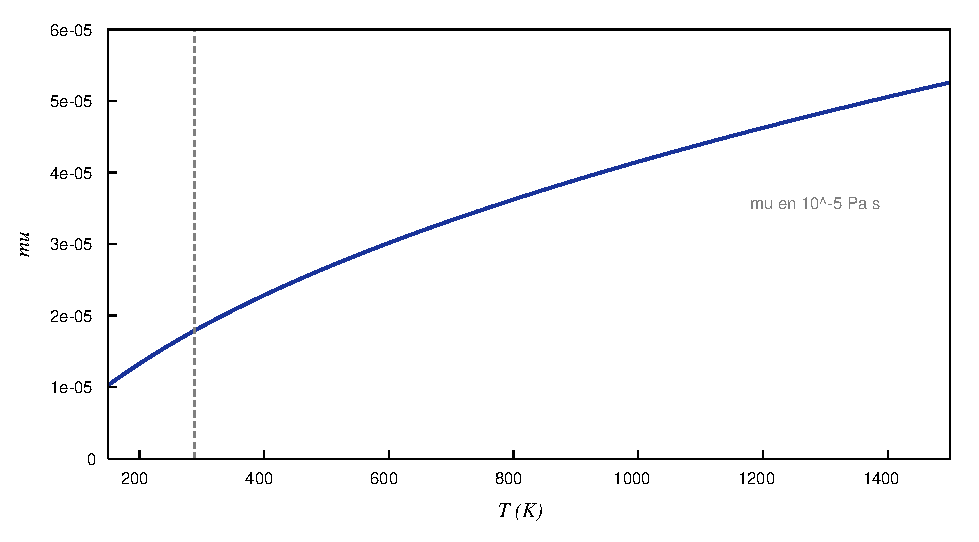
\includegraphics{../figures/FIG-0049/figure.pdf}}%
\count0=\ht0
\advance\count0 by \dp0
\count2=\wd0
\count4=\dimexpr\textheight/100*38\relax
\count6=\linewidth
\ifnum\count0<1
\count0=1
\fi
\ifnum\count2<1
\count2=1
\fi
\divide\count0 by 4096
\divide\count2 by 4096
\divide\count4 by 4096
\divide\count6 by 4096
\ifnum\count0<1
\count0=1
\fi
\ifnum\count2<1
\count2=1
\fi
\ifnum\count4<1
\count4=1
\fi
\ifnum\count6<1
\count6=1
\fi
\count8=\count2
\ifnum\count0>\count4
\count8=\numexpr\count2*\count4/\count0\relax
\fi
\ifnum\count8>\count6
\resizebox{\linewidth}{!}{\box0}%
\else
\ifnum\count0>\count4
\resizebox{!}{\dimexpr\textheight/100*38\relax}{\box0}%
\else
\box0%
\fi
\fi
\endgroup
\par\nopagebreak
\studiumcaption{fig:c03-sutherland}{Viscosidad dinámica del aire según la correlación de Sutherland con \(\mu_0 = 1.716\times 10^{-5}\) Pa s, \(T_0 = 273.15\) K y \(S = 110.4\) K, entre 150 y 1500 K. La línea discontinua marca 288.15 K.}
\end{minipage}
\par\vspace{\baselineskip}

La escala molecular relevante para el movimiento de un gas no es la separación entre moléculas, sino el recorrido libre medio \(\lambda\), distancia media que recorre una molécula entre dos choques; en el aire de la atmósfera estándar a nivel del mar vale \(6.63\times 10^{-8}\) m. El cociente entre \(\lambda\) y una longitud característica \(L\) del problema es el número de Knudsen,
\begin{equation}
\mathrm{Kn} = \frac{\lambda}{L}, \label{eq:c03-knudsen}
\end{equation}
que decide qué descripción es adecuada. De forma orientativa y empírica, para \(\mathrm{Kn} < 0.01\) el flujo es continuo; entre \(0.01\) y \(0.1\) se mantiene la descripción continua pero el gas desliza sobre las paredes; entre \(0.1\) y 10 el régimen es de transición, y por encima de 10 el flujo es molecular libre. Para una partícula de polvo de diez micrómetros en aire a nivel del mar, \(\mathrm{Kn} = 6.63\times 10^{-8}/1.0\times 10^{-5} = 6.63\times 10^{-3}\), en el límite del régimen continuo. El recorrido libre medio es inversamente proporcional a la densidad, de modo que crece rápidamente con la altitud: en la alta atmósfera alcanza milímetros, metros y, en órbita baja, kilómetros. Un satélite en órbita baja se mueve, por tanto, en régimen molecular libre, y su resistencia aerodinámica no puede calcularse con las ecuaciones de este libro; la reentrada de una cápsula atraviesa sucesivamente todos los regímenes. Este es el primer ejemplo de una idea que recorrerá el texto: cada modelo tiene un dominio de validez que se expresa mediante un grupo adimensional.

Conviene distinguir desde ahora entre el fluido real y los modelos que se usan para describirlo. Un fluido ideal, o no viscoso, es un modelo en el que se supone viscosidad nula; las únicas fuerzas de superficie que transmite son de presión, tanto si está en reposo como si se mueve. Un fluido perfecto, en la terminología habitual, ignora además la compresibilidad. Ningún fluido real es ideal, pero el modelo es extraordinariamente útil cuando los efectos viscosos quedan confinados a capas delgadas junto a las paredes, como ocurre en el flujo alrededor de un ala a número de Reynolds elevado; fuera de esas capas, el aire se comporta como un fluido ideal y la sustentación puede calcularse sin viscosidad. El modelo fracasa, en cambio, cuando se pregunta por la resistencia de fricción o por el desprendimiento de la corriente, que son consecuencias directas de la viscosidad. El fluido real más sencillo que incluye viscosidad es el fluido newtoniano, al que el aire y el agua se ajustan muy bien en condiciones ordinarias. Confundir el modelo con la realidad es el origen de paradojas célebres, como la de d'Alembert, según la cual un cuerpo que se mueve en un fluido ideal no experimenta resistencia; el capítulo 12 vuelve sobre ella.

\section{Fuerzas de volumen y de superficie}

Sobre una porción de fluido de volumen \(V\) limitada por una superficie \(S\) actúan dos tipos de fuerzas. Las fuerzas de volumen actúan a distancia sobre toda la masa contenida en \(V\); la más importante es el peso, pero también lo son las fuerzas electromagnéticas sobre un fluido conductor y, en un sistema de referencia no inercial, las fuerzas de inercia del capítulo 2. Se describen mediante una fuerza por unidad de masa \(\mathbf{f}_m\), de modo que la fuerza de volumen total es \(\int_V \rho\,\mathbf{f}_m\,dV\); en el caso gravitatorio \(\mathbf{f}_m = \mathbf{g}\). Las fuerzas de superficie son fuerzas de contacto que ejerce el medio exterior a través de la superficie \(S\); su intensidad se describe con el vector tensión \(\mathbf{t}\), fuerza por unidad de área, que depende del punto y de la orientación de la superficie, caracterizada por su normal exterior \(\mathbf{n}\). La fuerza de superficie total es \(\int_S \mathbf{t}\,dS\). El vector tensión tiene una componente normal a la superficie y otra tangencial, el esfuerzo cortante; ambas se miden en pascales. En un fluido en reposo, o en un fluido ideal, el vector tensión es puramente normal: \(\mathbf{t}\) vale \(-p\,\mathbf{n}\): el signo menos indica que la presión empuja hacia el interior de la porción de fluido. En el capítulo 13 se demostrará que, en general, el vector tensión depende linealmente de la normal a través del tensor de esfuerzos.

La diferencia de escala entre ambos tipos de fuerzas tiene una consecuencia que conviene entender cuanto antes. Si una porción de fluido tiene un tamaño característico \(\ell\), las fuerzas de volumen son proporcionales a \(\ell^{3}\) y las de superficie a \(\ell^{2}\). Al reducir \(\ell\) hacia cero, las fuerzas de volumen y la inercia, también proporcional a la masa, se anulan más deprisa que las de superficie. Por tanto, el equilibrio de un elemento infinitesimal exige que las fuerzas de superficie se equilibren por sí solas a primer orden. Este argumento, aplicado a un tetraedro elemental, es el que permite a Cauchy demostrar la existencia del tensor de esfuerzos, y aplicado a un fluido en reposo demuestra que la presión en un punto no depende de la orientación de la superficie sobre la que se evalúa. Es también la razón por la que, en ausencia de flujo, un gradiente de presión es la única fuerza de superficie neta capaz de equilibrar el peso, como se verá en la ecuación fundamental de la hidrostática.

\section{Viscosidad y fluidos newtonianos}

Cuando capas de fluido adyacentes se mueven a velocidades distintas, aparece entre ellas un esfuerzo tangencial que se opone al movimiento relativo. En los líquidos su origen son las fuerzas de cohesión entre moléculas; en los gases, el intercambio de cantidad de movimiento entre capas causado por la agitación molecular. Para un flujo cortante simple, en el que la velocidad \(u\) en la dirección \(x\) solo varía con la coordenada perpendicular \(y\), la ley de Newton de la viscosidad establece que
\begin{equation}
\tau = \mu\,\frac{du}{dy}, \label{eq:c03-newton}
\end{equation}
donde \(\mu\) es la viscosidad dinámica, cuya unidad en el SI es el pascal segundo. El ejemplo más simple es una película de fluido de espesor \(h\) entre una pared fija y una placa que se mueve paralelamente a ella con velocidad \(U\). Si no hay gradiente de presión en la dirección del movimiento, el perfil de velocidad es lineal, \(u = Uy/h\) (véase la figura~\ref{fig:c03-pelicula}), su derivada es uniforme y el esfuerzo vale \(\tau = \mu U/h\) en toda la película: la fuerza necesaria para arrastrar la placa es proporcional a la viscosidad, al área y a la velocidad, e inversamente proporcional al espesor. Este resultado, aplicado a la holgura entre un eje y su casquillo, permite estimar el par resistente y la potencia disipada en un cojinete lubricado, como se hace en el problema resuelto del capítulo.

En muchas ecuaciones la viscosidad aparece dividida por la densidad; ese cociente es la viscosidad cinemática, \(\nu = \mu/\rho\), con unidades de m\(^2\)/s, y tiene la interpretación física de una difusividad de cantidad de movimiento, como se verá en el capítulo 13. El agua a 20 \(^\circ\)C tiene \(\mu \approx 1.005\times 10^{-3}\) Pa s, del orden de un centipoise, y densidad \(998.2\) kg/m\(^3\), de modo que \(\nu = 1.005\times 10^{-3}/998.2 \approx 1.007\times 10^{-6}\) m\(^2\)/s. El aire de la atmósfera estándar a nivel del mar tiene una viscosidad dinámica unas cincuenta y seis veces menor, \(\mu = 1.7894\times 10^{-5}\) Pa s, pero como su densidad es unas ochocientas veces menor, su viscosidad cinemática, \(1.7894\times 10^{-5}/1.225 \approx 1.4607\times 10^{-5}\) m\(^2\)/s, es unas quince veces mayor que la del agua. Este hecho, a primera vista paradójico, es esencial en los ensayos con modelos del capítulo 10. La viscosidad depende fuertemente de la temperatura y muy poco de la presión, pero en sentido opuesto en líquidos y gases: en un líquido disminuye al calentarlo, porque se debilitan las fuerzas de cohesión, y en un gas aumenta, porque crece la agitación molecular. Para el aire, la fórmula de Sutherland,
\begin{equation}
\mu = \mu_0\left(\frac{T}{T_0}\right)^{3/2}\frac{T_0 + S}{T + S}, \label{eq:c03-sutherland}
\end{equation}
con \(S \approx 110.4\) K, reproduce bien los datos en un amplio intervalo de temperaturas; es una correlación semiempírica, basada en un modelo molecular simplificado y ajustada a medidas, no una ley exacta. La figura~\ref{fig:c03-sutherland} la representa.

Un fluido es newtoniano cuando el esfuerzo viscoso es proporcional a la velocidad de deformación con una viscosidad que solo depende del estado termodinámico, y no de la propia velocidad de deformación ni de la historia del flujo. El aire, el agua, los combustibles de aviación y los aceites minerales ligeros se comportan como newtonianos con gran aproximación. Existen, sin embargo, muchos fluidos no newtonianos: las pinturas y muchas disoluciones de polímeros reducen su viscosidad aparente al aumentar la velocidad de deformación, mientras que ciertas suspensiones concentradas la aumentan, y la sangre o los fluidos con umbral de fluencia muestran comportamientos aún más complejos. En este libro se adopta siempre el modelo newtoniano; su generalización a flujos tridimensionales arbitrarios, la ley de Navier-Poisson, se deduce en el capítulo 13 y, combinada con la segunda ley de Newton, conduce a las ecuaciones de Navier-Stokes.

\begin{tcolorbox}[title={Consejo}, studiumtip, breakable]

Antes de aplicar las ecuaciones del continuo a un problema poco habitual (microdispositivos, alta atmósfera, vacío), calcule el número de Knudsen con la longitud característica más pequeña del problema. Si supera aproximadamente 0,01, las condiciones de contorno de no deslizamiento dejan de ser exactas; si supera 0,1, el modelo continuo no es fiable.
\end{tcolorbox}

\begin{tcolorbox}[title={Definición}, studiumdef, breakable]

de fluido; fluidos ideales y reales
Un sólido sometido a un esfuerzo cortante se deforma una cantidad finita y queda en equilibrio, de modo que el esfuerzo está relacionado con la deformación. Un fluido, en cambio, se deforma de forma continua mientras actúe un esfuerzo cortante, por pequeño que sea: su módulo de cizalladura es nulo y el esfuerzo está relacionado con la velocidad de deformación, no con la deformación. De esta definición se sigue una consecuencia fundamental: un fluido en reposo no puede soportar esfuerzos cortantes, por lo que en equilibrio estático las únicas fuerzas de superficie son normales. La fuerza normal por unidad de área en un fluido en reposo es la presión, que se trata en detalle en el capítulo 5. Líquidos y gases son ambos fluidos, pero difieren en su compresibilidad: la densidad de un líquido apenas cambia con la presión, mientras que la de un gas es proporcional a ella a temperatura constante. Para el aire se usa casi siempre la ecuación de estado del gas ideal, \(p = \rho R_a T\), con \(R_a \approx 287.05\) J/(kg K) para el aire seco; en la atmósfera estándar a nivel del mar da \(\rho = 101\,325/(287.05\cdot 288.15) \approx 1.2250\) kg/m\(^3\).
\end{tcolorbox}

\begin{tcolorbox}[title={Definición}, studiumdef, breakable]

Viscosidad dinámica \(\mu\): constante de proporcionalidad entre el esfuerzo cortante y la velocidad de deformación en un flujo cortante simple, \(\tau = \mu\,du/dy\). Viscosidad cinemática: cociente \(\nu = \mu/\rho\), con dimensiones de difusividad.
\end{tcolorbox}



\section{Desarrollos y práctica}

Las deducciones que siguen cuantifican las dos hipótesis de partida del libro. La densidad de un gas ideal \(\eqref{eq:c03-densidad}\) y el número de Knudsen \(\eqref{eq:c03-knudsen}\) permiten decidir si el modelo de medio continuo es aplicable; la ley de Newton de la viscosidad \(\eqref{eq:c03-newton}\) y la ley de Sutherland \(\eqref{eq:c03-sutherland}\) dan el esfuerzo viscoso en un fluido newtoniano y su dependencia de la temperatura en los gases. El problema resuelto aplica la ley de Newton a una película de lubricante, y los ejercicios avanzados introducen geometrías de holgura delgada que el capítulo 15 justificará con la teoría de la lubricación. En todos ellos es importante distinguir la viscosidad dinámica de la cinemática y comprobar las unidades de cada término.

\begin{tcolorbox}[title={Desarrollos del modelo}, studiumdef, breakable]

\noindent\textbf{Densidad de un gas ideal}

\begin{equation}
\rho = \frac{p}{R_a T}
\label{eq:c03-gas-ideal}
\end{equation}

\noindent\textbf{Hipótesis}
\begin{itemize}
\item gas ideal
\item aire seco con composición fija
\end{itemize}

\noindent\textbf{Limitaciones}
\begin{itemize}
\item a presiones muy altas o temperaturas muy bajas el aire se aparta del comportamiento ideal
\end{itemize}

\noindent\textbf{Pasos}
\begin{enumerate}
\item
partir de la ecuación de estado p = rho \(R_a T\)

\[
p = \rho R_a T
\]
\item
despejar la densidad

\[
\rho = \frac{p}{R_a T}
\]
\end{enumerate}

\noindent\textbf{Variables}
\begin{itemize}
\item $R_{a}$: constante del aire seco ($\mathrm{J}\,\mathrm{kg}^{-1}\,\mathrm{K}^{-1}$)
\end{itemize}



\noindent\textbf{Densidad numérica de un gas ideal}

\begin{equation}
n_v = \frac{p}{k_B T}
\label{eq:c03-densidad-numerica}
\end{equation}

\noindent\textbf{Hipótesis}
\begin{itemize}
\item gas ideal
\end{itemize}

\noindent\textbf{Limitaciones}
\begin{itemize}
\item estimación de orden de magnitud para la escala molecular
\end{itemize}

\noindent\textbf{Pasos}
\begin{enumerate}
\item
escribir la ecuación de estado en forma molecular

\[
p = n_v k_B T
\]
\item
despejar el número de moléculas por unidad de volumen

\[
n_v = \frac{p}{k_B T}
\]
\end{enumerate}

\noindent\textbf{Variables}
\begin{itemize}
\item $n_{v}$: moléculas por unidad de volumen ($\mathrm{1/m^3}$)
\end{itemize}



\noindent\textbf{Esfuerzo cortante en una película de perfil lineal}

\begin{equation}
\tau = \mu\,\frac{U}{h}
\label{eq:c03-pelicula}
\end{equation}

\noindent\textbf{Hipótesis}
\begin{itemize}
\item fluido newtoniano
\item perfil de velocidad lineal entre una pared fija y una placa que se mueve con velocidad U
\item película de espesor h constante
\end{itemize}

\noindent\textbf{Limitaciones}
\begin{itemize}
\item el perfil es lineal solo si no hay gradiente de presión en la dirección del movimiento (capítulo 6)
\end{itemize}

\noindent\textbf{Pasos}
\begin{enumerate}
\item
el perfil lineal es u = U y / h

\[
u(y) = U\,\frac{y}{h}
\]
\item
su derivada es uniforme e igual a U/h

\[
\frac{du}{dy} = \frac{U}{h}
\]
\item
la ley de Newton da un esfuerzo uniforme en toda la película

\[
\tau = \mu\,\frac{du}{dy} = \mu\,\frac{U}{h}
\]
\item
relación usada en el texto (paso intermedio no comprobado por separado)

\[
u = Uy/h
\]
\end{enumerate}

\noindent\textbf{Variables}
\begin{itemize}
\item $U$: velocidad de la placa ($\mathrm{m}\,\mathrm{s}^{-1}$)
\item $h$: espesor de la película ($\mathrm{m}$)
\end{itemize}



\noindent\textbf{Par y potencia viscosos en un cojinete de holgura delgada}

\begin{equation}
M = \frac{2\pi\mu\,\omega R^{3} L}{c},\qquad \dot W = M\omega = \frac{2\pi\mu\,\omega^{2} R^{3} L}{c}
\label{eq:c03-petroff}
\end{equation}

\noindent\textbf{Hipótesis}
\begin{itemize}
\item eje concéntrico con el casquillo
\item holgura c mucho menor que el radio R
\item perfil lineal en la holgura
\end{itemize}

\noindent\textbf{Limitaciones}
\begin{itemize}
\item ignora la excentricidad del eje cargado y los efectos de extremo
\end{itemize}

\noindent\textbf{Pasos}
\begin{enumerate}
\item
el esfuerzo en la holgura es mu omega R / c

\[
\tau = \mu\,\frac{\omega R}{c}
\]
\item
se multiplica por el área lateral 2 pi R L y por el brazo R

\[
M = \tau\,(2\pi R L)\,R
\]
\item
la potencia disipada es el par por la velocidad angular

\[
\dot W = M\,\omega
\]
\end{enumerate}

\noindent\textbf{Variables}
\begin{itemize}
\item $c$: holgura radial ($\mathrm{m}$)
\item $L$: longitud del cojinete ($\mathrm{m}$)
\end{itemize}


\end{tcolorbox}

\begin{tcolorbox}[title={Problema resuelto}, studiumworked, breakable]

\noindent\textbf{Enunciado}
Un eje de 50 mm de diámetro gira a 3000 rpm dentro de un casquillo de 80 mm de longitud. La holgura radial, uniforme, es \(c = 0.10\) mm y está llena de un aceite de viscosidad \(\mu = 0.030\) Pa s. Suponiendo un perfil de velocidad lineal en la holgura, calcule el esfuerzo cortante en la superficie del eje, el par resistente y la potencia disipada por fricción viscosa.

\noindent\textbf{Datos}
\begin{itemize}
\item $\mu = 0.03\,\mathrm{Pa}\,\mathrm{s}$ — viscosidad del aceite
\item $\omega = 314.159\,\mathrm{rad}\,\mathrm{s}^{-1}$ — velocidad angular (3000 rpm)
\item $R = 0.025\,\mathrm{m}$ — radio del eje
\item $L = 0.08\,\mathrm{m}$ — longitud del casquillo
\item $c = 0.0001\,\mathrm{m}$ — holgura radial
\end{itemize}

\noindent\textbf{Incógnita}
potencia disipada en el cojinete

\noindent\textbf{Modelo físico}

\noindent\textit{Potencia viscosa en una holgura delgada}

\[
\dot W = \frac{2\pi\mu\,\omega^{2} R^{3} L}{c}
\]

\noindent\textbf{Hipótesis}
\begin{itemize}
\item eje concéntrico
\item c mucho menor que R, de modo que la curvatura de la holgura es despreciable
\item perfil lineal y fluido newtoniano
\item viscosidad uniforme (sin calentamiento)
\end{itemize}

\noindent\textbf{Desarrollo paso a paso}

\phantomsection\label{solution:mf-003}
\noindent\textbf{Elección del procedimiento.} La pared del eje arrastra el aceite a $U=\omega R$ y la carcasa permanece fija. En una holgura delgada el gradiente es $U/c$. La ley newtoniana da el esfuerzo; su integral sobre el área mojada da fuerza, y multiplicar por el brazo $R$ da par.

\begin{enumerate}

\item Convertir las revoluciones por minuto antes de usar la velocidad angular.

\[\fitmath{\mathrm{om}=\frac{2\cdot \pi\cdot N}{60}}\]

\[\fitmath{\mathrm{om}=\frac{2\cdot \pi\cdot (3000)}{60}\approx 314{,}1593\,\mathrm{1/s}}\]

\item Pasar de velocidad angular a velocidad de la pared.

\[\fitmath{U=\mathrm{om}\cdot R}\]

\[\fitmath{U=(314{,}1592654)\cdot (0{,}025)\approx 7{,}853982\,\mathrm{m/s}}\]

\item Aplicar $\tau=\mu\,du/dy$ con perfil lineal.

\[\fitmath{\tau=\frac{\mu\cdot U}{c}}\]

\[\fitmath{\tau=\frac{(0{,}03)\cdot (7{,}853981634)}{(0{,}0001)}\approx 2356{,}194\,\mathrm{Pa}}\]

\item El área mojada es $2\pi RL$ y el brazo es $R$.

\[\fitmath{M=\tau\cdot 2\cdot \pi\cdot R\cdot L\cdot R}\]

\[\fitmath{M=(2356{,}19449)\cdot 2\cdot \pi\cdot (0{,}025)\cdot (0{,}08)\cdot (0{,}025)\approx 0{,}7402203\,\mathrm{N\,m}}\]

\item La potencia mecánica del par es $M\omega$.

\[\fitmath{P=M\cdot \mathrm{om}}\]

\[\fitmath{P=(0{,}7402203301)\cdot (314{,}1592654)\approx 232{,}5471\,\mathrm{W}}\]

\end{enumerate}


\noindent\textbf{Sustitución numérica}

\[
\frac{2 \pi \left(0.08\,\mathrm{m}\right) \left(0.025\,\mathrm{m}\right)^{3} \left(0.03\,\mathrm{Pa}\,\mathrm{s}\right) \left(\left(314.159\,\mathrm{rad}\,\mathrm{s}^{-1}\right)\right)^{2}}{\left(0.0001\,\mathrm{m}\right)}
\]

\noindent\textbf{Resultado}

\[
\tau \approx 2.36\ \mathrm{kPa},\quad M \approx 0.740\ \mathrm{N\,m},\quad \dot W \approx 233\ \mathrm{W}
\]

\noindent\textbf{Interpretación}
Más de 200 W se convierten en calor en un único cojinete; por eso los cojinetes de turbomáquinas necesitan circuitos de refrigeración del aceite, y la viscosidad real disminuye al calentarse.

\noindent\textbf{Comprobación de la respuesta} la aritmética del último paso reproduce la respuesta enunciada a la precisión con que está escrita. Es una reproducción aritmética; no valida el modelo físico ni sus hipótesis.

\noindent\textbf{Limitaciones}
\begin{itemize}
\item un eje cargado es excéntrico y el modelo de Petroff subestima la fricción
\item la viscosidad del aceite depende mucho de la temperatura
\end{itemize}

\noindent\textbf{Errores frecuentes}
\begin{itemize}
\item usar el diámetro en lugar del radio en la velocidad periférica
\item olvidar multiplicar por el brazo R para obtener el par
\end{itemize}
\end{tcolorbox}

\begin{tcolorbox}[title={Ejercicios propuestos}, studiumworked, breakable]

\noindent\textbf{1 (Básico, Cálculo)}
En un aeródromo de montaña la presión es \(79.5\) kPa y la temperatura 2 \(^\circ\)C. Calcule la densidad del aire con la ecuación de estado del gas ideal (\(R_a = 287.05\) J/(kg K)) y compárela con la del nivel del mar estándar.

\noindent\textbf{2 (Básico, Interpretación)}
A cierta altitud de la mesosfera el recorrido libre medio del aire es de unos \(4.4\) mm. Una sonda de reentrada tiene un diámetro de \(0.50\) m. Calcule el número de Knudsen basado en el diámetro e indique el régimen de flujo según la clasificación orientativa del capítulo.

\noindent\textbf{3 (Intermedio, Aplicación)}
Con la fórmula de Sutherland, \(\mu_0 = 1.716\times 10^{-5}\) Pa s a \(T_0 = 273.15\) K y \(S = 110.4\) K, estime la viscosidad del aire a 1000 K, temperatura típica a la salida de la cámara de combustión diluida de una turbina. ¿Cuántas veces mayor es que a 288 K?

\noindent\textbf{4 (Avanzado, COMPARATIVE)}
Compare la viscosidad cinemática del aire estándar a nivel del mar (\(\mu = 1.7894\times 10^{-5}\) Pa s, \(\rho = 1.225\) kg/m\(^3\)) con la del agua a 20 \(^\circ\)C (\(\mu = 1.005\times 10^{-3}\) Pa s, \(\rho = 998.2\) kg/m\(^3\)). Calcule el cociente entre ambas y explique qué significa que el aire sea más viscoso en términos cinemáticos.

\noindent\textbf{5 (De examen, DESIGN)}
Un viscosímetro de cilindros coaxiales tiene un cilindro interior de radio 40 mm y altura útil 100 mm que gira a 10 rad/s; la holgura con el cilindro exterior es de \(2.0\) mm. Se mide un par de \(0.12\) N m. Suponiendo perfil lineal en la holgura y despreciando los efectos de fondo, determine la viscosidad del fluido.

\noindent\textbf{6 (Intermedio, Cálculo)}
Una placa de \(0.50\) m\(^2\) se arrastra a \(2.0\) m/s sobre una película de aceite de \(1.0\) mm de espesor y viscosidad \(0.29\) Pa s apoyada en una superficie fija. Suponiendo perfil lineal, calcule la fuerza necesaria.
\end{tcolorbox}

\begin{tcolorbox}[title={Autoevaluación}, studiumcheck, breakable]

(1) ¿Por qué no tiene sentido hablar de la densidad en un punto a escala molecular, y cómo resuelve el problema la hipótesis del continuo? (2) Explique con el número de Knudsen por qué un satélite en órbita baja no puede estudiarse con las ecuaciones de Navier-Stokes. (3) ¿Qué propiedad distingue a un fluido de un sólido? (4) Dé un ejemplo en el que el modelo de fluido ideal funciona y otro en el que falla. (5) ¿Por qué la viscosidad de un gas aumenta con la temperatura y la de un líquido disminuye? (6) ¿Cuál tiene mayor viscosidad cinemática, el aire o el agua, y qué implica para un ensayo con modelos?
\end{tcolorbox}
\studiumchaptercheck

\chapter{Descripción del movimiento de un fluido}
\label{chap:c04}

\studiumchapterguide{Antes de preguntarse por las fuerzas que mueven un fluido hay que saber describir su movimiento. Este capítulo presenta las dos descripciones posibles, la lagrangiana, que sigue a cada partícula, y la euleriana, que observa puntos fijos del espacio; define las tres familias de curvas con que se visualiza un flujo, que solo coinciden en flujo estacionario; deduce la derivada material, la herramienta que traduce las leyes de la mecánica, formuladas para partículas, al lenguaje de campos, y termina con la clasificación de los flujos y las condiciones iniciales y de contorno que completan cualquier planteamiento.}

\section{Descripciones lagrangiana y euleriana}

En la descripción lagrangiana se identifica cada partícula de fluido por una etiqueta, normalmente su posición \(\boldsymbol{\xi}\) en un instante inicial \(t_0\), y se describe el movimiento mediante la función \(\mathbf{x} = \mathbf{X}(\boldsymbol{\xi}, t)\), que da la posición en el instante \(t\) de la partícula que en \(t_0\) estaba en \(\boldsymbol{\xi}\). Es la descripción natural de la mecánica de partículas del capítulo 1, y en ella la velocidad y la aceleración de una partícula son simplemente \(\partial\mathbf{X}/\partial t\) y \(\partial^{2}\mathbf{X}/\partial t^{2}\) a etiqueta fija. Equivale a sentarse en una barca y dejarse llevar por la corriente. En la descripción euleriana, en cambio, las variables independientes son la posición \(\mathbf{x}\) de un punto fijo del espacio y el tiempo, y el flujo se describe con campos como la velocidad \(\mathbf{u}(\mathbf{x}, t)\), la presión \(p(\mathbf{x}, t)\) o la densidad \(\rho(\mathbf{x}, t)\): es lo que ve un observador sentado en la orilla. Las dos descripciones están ligadas por la condición de que la velocidad euleriana en el punto donde se encuentra una partícula coincida con la velocidad de esa partícula,
\begin{equation}
\frac{\partial \mathbf{X}}{\partial t}(\boldsymbol{\xi}, t) = \mathbf{u}\big(\mathbf{X}(\boldsymbol{\xi}, t), t\big). \label{eq:c04-enlace}
\end{equation}
Dado el campo euleriano, la ecuación \(\eqref{eq:c04-enlace}\) es un sistema de ecuaciones diferenciales ordinarias cuya solución, con la condición inicial \(\mathbf{X} = \boldsymbol{\xi}\) en \(t_0\), proporciona la descripción lagrangiana. La mecánica de fluidos usa casi siempre la descripción euleriana, porque los instrumentos (una sonda de presión, un anemómetro, un tubo de Pitot) miden en puntos fijos y porque las condiciones de contorno se imponen en superficies fijas; pero las leyes físicas se aplican a partículas, de modo que hace falta un puente entre ambas. Ninguna de las dos descripciones está ligada a un sistema de referencia concreto: ambas pueden usarse en cualquier sistema, inercial o no.

\par\vspace{\baselineskip}
\noindent\begin{minipage}{\linewidth}
\centering
\begingroup
\setbox0=\hbox{\begin{tikzpicture}
\draw[->] (0,0) -- (5.4,0) node[right]{$x$};
\draw[->] (0,0) -- (0,4.6) node[above]{$y$};
\draw[very thick,black] (0,0) -- (4.4,4.4) node[above]{línea de corriente};
\draw[very thick,red,domain=0:1,samples=40] plot ({4*\x},{4*\x*\x/2});
\draw[very thick,blue,domain=0:1,samples=40] plot ({4*\x},{4*(\x - \x*\x/2)});
\fill (4,2) circle (2pt);
\node[red,right] at (3.3,1.0) {trayectoria};
\node[blue,above left] at (2.2,1.5) {traza};
\draw[dotted] (4,0) node[below]{$x = u_0 t$} -- (4,4);
\end{tikzpicture}}%
\count0=\ht0
\advance\count0 by \dp0
\count2=\wd0
\count4=\dimexpr\textheight/100*38\relax
\count6=\linewidth
\ifnum\count0<1
\count0=1
\fi
\ifnum\count2<1
\count2=1
\fi
\divide\count0 by 4096
\divide\count2 by 4096
\divide\count4 by 4096
\divide\count6 by 4096
\ifnum\count0<1
\count0=1
\fi
\ifnum\count2<1
\count2=1
\fi
\ifnum\count4<1
\count4=1
\fi
\ifnum\count6<1
\count6=1
\fi
\count8=\count2
\ifnum\count0>\count4
\count8=\numexpr\count2*\count4/\count0\relax
\fi
\ifnum\count8>\count6
\resizebox{\linewidth}{!}{\begin{tikzpicture}
\draw[->] (0,0) -- (5.4,0) node[right]{$x$};
\draw[->] (0,0) -- (0,4.6) node[above]{$y$};
\draw[very thick,black] (0,0) -- (4.4,4.4) node[above]{línea de corriente};
\draw[very thick,red,domain=0:1,samples=40] plot ({4*\x},{4*\x*\x/2});
\draw[very thick,blue,domain=0:1,samples=40] plot ({4*\x},{4*(\x - \x*\x/2)});
\fill (4,2) circle (2pt);
\node[red,right] at (3.3,1.0) {trayectoria};
\node[blue,above left] at (2.2,1.5) {traza};
\draw[dotted] (4,0) node[below]{$x = u_0 t$} -- (4,4);
\end{tikzpicture}}%
\else
\ifnum\count0>\count4
\resizebox{!}{\dimexpr\textheight/100*38\relax}{\begin{tikzpicture}
\draw[->] (0,0) -- (5.4,0) node[right]{$x$};
\draw[->] (0,0) -- (0,4.6) node[above]{$y$};
\draw[very thick,black] (0,0) -- (4.4,4.4) node[above]{línea de corriente};
\draw[very thick,red,domain=0:1,samples=40] plot ({4*\x},{4*\x*\x/2});
\draw[very thick,blue,domain=0:1,samples=40] plot ({4*\x},{4*(\x - \x*\x/2)});
\fill (4,2) circle (2pt);
\node[red,right] at (3.3,1.0) {trayectoria};
\node[blue,above left] at (2.2,1.5) {traza};
\draw[dotted] (4,0) node[below]{$x = u_0 t$} -- (4,4);
\end{tikzpicture}}%
\else
\begin{tikzpicture}
\draw[->] (0,0) -- (5.4,0) node[right]{$x$};
\draw[->] (0,0) -- (0,4.6) node[above]{$y$};
\draw[very thick,black] (0,0) -- (4.4,4.4) node[above]{línea de corriente};
\draw[very thick,red,domain=0:1,samples=40] plot ({4*\x},{4*\x*\x/2});
\draw[very thick,blue,domain=0:1,samples=40] plot ({4*\x},{4*(\x - \x*\x/2)});
\fill (4,2) circle (2pt);
\node[red,right] at (3.3,1.0) {trayectoria};
\node[blue,above left] at (2.2,1.5) {traza};
\draw[dotted] (4,0) node[below]{$x = u_0 t$} -- (4,4);
\end{tikzpicture}%
\fi
\fi
\endgroup
\par\nopagebreak
\studiumcaption{fig:c04-lineas}{Flujo \(u = u_0\), \(v = at\) con \(u_0 = a = 1\) (unidades arbitrarias) en el instante \(t = 1\): línea de corriente que pasa por el origen (recta), trayectoria de la partícula que pasó por el origen en \(t = 0\) (parábola inferior) y traza del colorante inyectado en el origen desde \(t = 0\) (parábola superior). Trayectoria y traza terminan en el mismo punto, ocupado por la primera partícula marcada.}
\end{minipage}
\par\vspace{\baselineskip}

\par\vspace{\baselineskip}
\noindent\begin{minipage}{\linewidth}
\centering
\begingroup
\setbox0=\hbox{\begin{tikzpicture}
\draw[->] (-3.2,0) -- (3.4,0) node[right]{$x$};
\draw[->] (0,0) -- (0,3.4) node[above]{$y$};
\fill[gray!30] (-3.2,-0.25) rectangle (3.2,0);
\foreach \c in {0.25,0.6,1.1,1.8} {
  \draw[thick,blue,domain={\c/3}:3,samples=60] plot (\x,{\c/\x});
  \draw[thick,blue,domain={-3}:{-\c/3},samples=60] plot (\x,{-\c/\x});
}
\draw[->,thick,blue] (1.0,1.1) -- (1.25,0.88);
\draw[->,thick,blue] (-1.0,1.1) -- (-1.25,0.88);
\fill (0,0) circle (2pt) node[below left]{$O$};
\end{tikzpicture}}%
\count0=\ht0
\advance\count0 by \dp0
\count2=\wd0
\count4=\dimexpr\textheight/100*38\relax
\count6=\linewidth
\ifnum\count0<1
\count0=1
\fi
\ifnum\count2<1
\count2=1
\fi
\divide\count0 by 4096
\divide\count2 by 4096
\divide\count4 by 4096
\divide\count6 by 4096
\ifnum\count0<1
\count0=1
\fi
\ifnum\count2<1
\count2=1
\fi
\ifnum\count4<1
\count4=1
\fi
\ifnum\count6<1
\count6=1
\fi
\count8=\count2
\ifnum\count0>\count4
\count8=\numexpr\count2*\count4/\count0\relax
\fi
\ifnum\count8>\count6
\resizebox{\linewidth}{!}{\begin{tikzpicture}
\draw[->] (-3.2,0) -- (3.4,0) node[right]{$x$};
\draw[->] (0,0) -- (0,3.4) node[above]{$y$};
\fill[gray!30] (-3.2,-0.25) rectangle (3.2,0);
\foreach \c in {0.25,0.6,1.1,1.8} {
  \draw[thick,blue,domain={\c/3}:3,samples=60] plot (\x,{\c/\x});
  \draw[thick,blue,domain={-3}:{-\c/3},samples=60] plot (\x,{-\c/\x});
}
\draw[->,thick,blue] (1.0,1.1) -- (1.25,0.88);
\draw[->,thick,blue] (-1.0,1.1) -- (-1.25,0.88);
\fill (0,0) circle (2pt) node[below left]{$O$};
\end{tikzpicture}}%
\else
\ifnum\count0>\count4
\resizebox{!}{\dimexpr\textheight/100*38\relax}{\begin{tikzpicture}
\draw[->] (-3.2,0) -- (3.4,0) node[right]{$x$};
\draw[->] (0,0) -- (0,3.4) node[above]{$y$};
\fill[gray!30] (-3.2,-0.25) rectangle (3.2,0);
\foreach \c in {0.25,0.6,1.1,1.8} {
  \draw[thick,blue,domain={\c/3}:3,samples=60] plot (\x,{\c/\x});
  \draw[thick,blue,domain={-3}:{-\c/3},samples=60] plot (\x,{-\c/\x});
}
\draw[->,thick,blue] (1.0,1.1) -- (1.25,0.88);
\draw[->,thick,blue] (-1.0,1.1) -- (-1.25,0.88);
\fill (0,0) circle (2pt) node[below left]{$O$};
\end{tikzpicture}}%
\else
\begin{tikzpicture}
\draw[->] (-3.2,0) -- (3.4,0) node[right]{$x$};
\draw[->] (0,0) -- (0,3.4) node[above]{$y$};
\fill[gray!30] (-3.2,-0.25) rectangle (3.2,0);
\foreach \c in {0.25,0.6,1.1,1.8} {
  \draw[thick,blue,domain={\c/3}:3,samples=60] plot (\x,{\c/\x});
  \draw[thick,blue,domain={-3}:{-\c/3},samples=60] plot (\x,{-\c/\x});
}
\draw[->,thick,blue] (1.0,1.1) -- (1.25,0.88);
\draw[->,thick,blue] (-1.0,1.1) -- (-1.25,0.88);
\fill (0,0) circle (2pt) node[below left]{$O$};
\end{tikzpicture}%
\fi
\fi
\endgroup
\par\nopagebreak
\studiumcaption{fig:c04-remanso}{Trayectorias del flujo plano de punto de remanso \(u = kx\), \(v = -ky\): hipérbolas \(xy = \mathrm{cte}\). El fluido llega por el eje \(y\), se frena en el origen y se acelera a lo largo del eje \(x\).}
\end{minipage}
\par\vspace{\baselineskip}

Un ejemplo sencillo ilustra el paso de una descripción a otra. El flujo plano y estacionario \(u = kx\), \(v = -ky\), con \(k\,>\,0\), describe el movimiento cerca del punto de remanso situado delante de un cuerpo romo: el fluido llega a lo largo del eje \(y\), se frena y se desvía a lo largo del eje \(x\). Integrando \(dx/dt = kx\) y \(dy/dt = -ky\) con la condición inicial \((x_0, y_0)\) se obtiene \(x(t) = x_0 e^{kt}\) e \(y(t) = y_0 e^{-kt}\), y eliminando el tiempo resulta que cada partícula se mueve sobre la hipérbola \(xy = x_0 y_0\). Aunque el campo euleriano no depende del tiempo, cada partícula acelera: su componente \(x\) crece exponencialmente mientras se aleja del punto de remanso. Este hecho, aparentemente contradictorio, es la primera manifestación de la aceleración convectiva que se estudia más adelante en este capítulo. La figura~\ref{fig:c04-remanso} muestra las hipérbolas.

\section{Líneas de corriente, trayectorias y trazas}

Para visualizar un flujo se usan tres familias de curvas. Las líneas de corriente son, en un instante dado, las curvas tangentes en cada punto al vector velocidad; si \(d\mathbf{x}\) es un elemento de una de ellas, debe ser paralelo a \(\mathbf{u}\), lo que en coordenadas cartesianas se escribe
\begin{equation}
\frac{dx}{u(\mathbf{x}, t)} = \frac{dy}{v(\mathbf{x}, t)} = \frac{dz}{w(\mathbf{x}, t)}, \qquad t\ \text{fijo}. \label{eq:c04-lineas}
\end{equation}
Dos líneas de corriente distintas no pueden cortarse en un punto donde la velocidad no sea nula, porque una partícula no puede tener dos velocidades a la vez; en los puntos de remanso, donde \(\mathbf{u} = \mathbf{0}\), sí pueden encontrarse. Las trayectorias son las curvas que recorren las partículas a lo largo del tiempo, soluciones del sistema que iguala la velocidad de cada partícula, \(d\mathbf{x}/dt\), al campo \(\mathbf{u}(\mathbf{x}, t)\) evaluado en su posición; a diferencia de las líneas de corriente, dependen de toda la historia del flujo y pueden cortarse entre sí y consigo mismas. Las trazas son el lugar geométrico, en un instante dado, de todas las partículas que han pasado por un mismo punto fijo: es lo que se observa al inyectar colorante o humo de forma continua desde un punto, como en los túneles de humo.

En un flujo estacionario las tres familias coinciden: cada partícula que pasa por un punto sigue la misma línea de corriente que las anteriores, de modo que trayectoria, traza y línea de corriente son la misma curva. En un flujo no estacionario son distintas, y confundirlas conduce a interpretaciones erróneas de las visualizaciones. Consideremos el campo uniforme en el espacio pero variable en el tiempo \(u = u_0\), \(v = at\), con \(u_0\) y \(a\) constantes. En el instante \(t\), todas las líneas de corriente son rectas de pendiente \(at/u_0\). La partícula que pasa por el origen en \(t = 0\) sigue la trayectoria \(x = u_0 t\), \(y = at^{2}/2\), es decir, la parábola \(y = ax^{2}/(2u_0^{2})\). La partícula que pasa por el origen en un instante posterior \(\tau\) se encuentra en \(t\) en \(x = u_0(t - \tau)\), \(y = a(t^{2} - \tau^{2})/2\); eliminando \(\tau\), la traza del colorante inyectado en el origen es
\begin{equation}
y = \frac{a}{2}\left(\frac{2 t x}{u_0} - \frac{x^{2}}{u_0^{2}}\right), \qquad 0 \le x \le u_0 t, \label{eq:c04-traza}
\end{equation}
una parábola con la concavidad opuesta a la de la trayectoria. La figura~\ref{fig:c04-lineas} representa las tres curvas en el instante \(t = 1\) para \(u_0 = a = 1\) en unidades arbitrarias. Una fotografía del humo en este flujo mostraría una curva que no es ni la trayectoria de ninguna partícula ni una línea de corriente.

\section{Derivada material y aceleración}

Sea \(\phi(\mathbf{x}, t)\) un campo euleriano cualquiera, por ejemplo la temperatura. La tasa de variación de \(\phi\) que experimenta una partícula de fluido no es \(\partial\phi/\partial t\), que es la variación en un punto fijo, sino la derivada de \(\phi\) evaluada sobre la trayectoria de la partícula. Aplicando la regla de la cadena a \(\phi(\mathbf{X}(\boldsymbol{\xi}, t), t)\) y usando la ecuación \(\eqref{eq:c04-enlace}\),
\begin{equation}
\frac{D\phi}{Dt} \equiv \frac{\partial \phi}{\partial t} + \mathbf{u}\cdot\nabla\phi = \frac{\partial \phi}{\partial t} + u\frac{\partial \phi}{\partial x} + v\frac{\partial \phi}{\partial y} + w\frac{\partial \phi}{\partial z}. \label{eq:c04-material}
\end{equation}
Este operador es la derivada material, también llamada sustancial o convectiva. El primer término es la derivada local, debida a que el campo cambia con el tiempo en un punto fijo; el segundo, el término convectivo, se debe a que la partícula se desplaza a regiones donde el campo tiene otro valor. Si en un conducto la temperatura es estacionaria pero aumenta a lo largo del eje con un gradiente \(G\), una partícula que avanza con velocidad \(u\) se calienta a razón \(uG\), que es el valor de \(DT/Dt\), aunque ningún termómetro fijo registre cambios. La derivada material es el puente entre descripciones: las leyes de la mecánica, que hablan de partículas, se escriben en forma euleriana sustituyendo \(d/dt\) por \(D/Dt\).

Aplicando la ecuación \(\eqref{eq:c04-material}\) a cada componente de la velocidad se obtiene la aceleración de una partícula de fluido,
\begin{equation}
\mathbf{a} = \frac{D\mathbf{u}}{Dt} = \frac{\partial \mathbf{u}}{\partial t} + (\mathbf{u}\cdot\nabla)\mathbf{u}, \label{eq:c04-aceleracion}
\end{equation}
suma de una aceleración local y de una aceleración convectiva. El término convectivo es no lineal en la velocidad y es la fuente de casi todas las dificultades matemáticas de la mecánica de fluidos, incluida la turbulencia. Su efecto se aprecia en una tobera convergente en la que la velocidad a lo largo del eje crece linealmente, \(u = U_0(1 + x/L)\). El flujo es estacionario, de modo que la aceleración local es nula, pero la aceleración convectiva vale \(u\,\partial u/\partial x = (U_0^{2}/L)(1 + x/L)\). Con \(U_0 = 50\) m/s y \(L = 2\) m, una partícula experimenta a la salida, en \(x = L\), una aceleración \((U_0^{2}/L)(1 + L/L)\) de 2500 m/s\(^2\), unas 255 veces la gravedad, en un flujo perfectamente estacionario. El resultado puede comprobarse por la vía lagrangiana: integrando \(dX/dt = U_0(1 + X/L)\) se obtiene \(X(t) = L[(1 + x_0/L)e^{U_0 t/L} - 1]\) y derivando dos veces se recupera exactamente la expresión anterior, comprobación que se ha realizado simbólicamente para este capítulo.

\section{Clasificación de flujos y condiciones de contorno}

Un flujo es estacionario si sus campos no dependen del tiempo, y no estacionario en caso contrario. La propiedad depende del sistema de referencia: el flujo alrededor de un avión que vuela con velocidad constante es no estacionario visto desde el suelo y estacionario visto desde el avión, y por eso casi siempre se estudia en ejes ligados al cuerpo. Un flujo es incompresible si la densidad de cada partícula permanece constante, es decir, si \(D\rho/Dt\) es nula; en el capítulo 12 se demostrará, a partir de la conservación de la masa, que esta condición equivale a que la divergencia del campo de velocidades sea nula, \(\nabla\cdot\mathbf{u} = 0\). Los líquidos suelen fluir de forma incompresible, pero también los gases a baja velocidad: la variación relativa de densidad que provoca un flujo de número de Mach \(\mathrm{Ma}\) es del orden de \(\mathrm{Ma}^{2}/2\), de modo que para \(\mathrm{Ma} = 0.3\) vale aproximadamente \(0.3^{2}/2\), es decir, 0,045, un 4.5 \%. Por eso el criterio práctico habitual es tratar como incompresible el flujo de aire con \(\mathrm{Ma} < 0.3\), es decir, por debajo de unos 100 m/s en condiciones de nivel del mar; a mayor velocidad la compresibilidad modifica apreciablemente las fuerzas aerodinámicas. Obsérvese la distinción: un fluido puede ser compresible y su flujo, incompresible.

Un flujo es unidimensional, bidimensional o tridimensional según el número de coordenadas espaciales de las que dependen sus campos. El flujo en un tubo largo y recto depende solo de la distancia al eje; el flujo alrededor de un ala de envergadura muy grande es aproximadamente plano, y el flujo alrededor de un cuerpo de revolución alineado con la corriente es axisimétrico, bidimensional en coordenadas cilíndricas. Estas simplificaciones reducen drásticamente la dificultad matemática y se usarán en los capítulos 6, 12 y 15. Más importante aún es la distinción entre flujo laminar y turbulento. En un flujo laminar las partículas siguen trayectorias suaves y ordenadas, deslizándose en capas que apenas se mezclan; en un flujo turbulento la velocidad y la presión fluctúan de forma caótica, aparecen remolinos de muchos tamaños que interaccionan entre sí y el transporte transversal de cantidad de movimiento, calor y masa aumenta enormemente, y con él la fricción. El paso de un régimen a otro está gobernado por el número de Reynolds, cociente entre los efectos de inercia y los viscosos, que se introduce en el capítulo 10: la turbulencia aparece cuando la energía cinética del flujo supera la capacidad amortiguadora de la viscosidad. La mayoría de los flujos de interés en ingeniería aeroespacial son turbulentos, al menos en parte.

Las ecuaciones del movimiento de un fluido son ecuaciones en derivadas parciales, y su solución exige condiciones iniciales, que especifican los campos en un instante de partida en problemas no estacionarios, y condiciones de contorno en todas las fronteras del dominio. En una pared sólida impermeable, la componente normal de la velocidad relativa a la pared debe ser nula; si el fluido es viscoso, además, la componente tangencial también lo es: es la condición de no deslizamiento, \(\mathbf{u} = \mathbf{u}_{\mathrm{pared}}\). Se trata de una condición empírica, confirmada en innumerables experimentos para fluidos newtonianos en régimen continuo, que falla cuando el número de Knudsen deja de ser pequeño. Su consecuencia es la existencia de una capa delgada junto a las paredes, la capa límite, en la que la velocidad pasa de cero en la superficie al valor de la corriente exterior. En un fluido ideal, en cambio, solo puede imponerse la impermeabilidad y el fluido desliza sobre la pared; esta pérdida de una condición de contorno es la raíz matemática de las limitaciones del modelo no viscoso. Otras condiciones habituales son las de corriente uniforme lejos de un cuerpo, las de entrada y salida en conductos y, en superficies libres, la continuidad de la presión y la condición cinemática de que la superficie esté formada siempre por las mismas partículas.

La derivada material aplicada a la propia velocidad da la aceleración de la partícula fluida, y conviene saber escribirla de tres formas equivalentes, porque cada una es la más cómoda en un tipo de problema. Con notación de índices, la componente \(i\) es \(a_i = \frac{\partial u_i}{\partial t} + u_j\,\frac{\partial u_i}{\partial x_j}\), con suma sobre \(j\). En dos dimensiones, las nueve derivadas del tensor gradiente de velocidad se reducen a cuatro y la aceleración convectiva es el producto de la matriz de esas derivadas por el vector velocidad,
\begin{equation}
\begin{pmatrix} a_x \\ a_y \end{pmatrix} = \frac{\partial}{\partial t}\begin{pmatrix} u \\ v \end{pmatrix} + \begin{pmatrix} \partial u/\partial x & \partial u/\partial y \\ \partial v/\partial x & \partial v/\partial y \end{pmatrix}\begin{pmatrix} u \\ v \end{pmatrix}, \label{eq:c04-matricial}
\end{equation}
forma muy útil para organizar los cálculos a mano o con un programa de cálculo simbólico. La tercera forma, vectorial, separa el gradiente de la energía cinética por unidad de masa y el efecto de la vorticidad: \((\mathbf{u}\cdot\nabla)\mathbf{u} = \nabla\!\left(\tfrac12|\mathbf{u}|^{2}\right) - \mathbf{u}\times\boldsymbol{\omega}\). Hay que insistir en una confusión frecuente: en un flujo estacionario la velocidad en cada punto fijo no cambia, pero la de cada partícula sí, porque la partícula se desplaza a puntos con velocidades distintas. Estacionario significa que se anula la derivada local \(\partial\mathbf{u}/\partial t\), no la derivada material \(D\mathbf{u}/Dt\).

Ejemplo. El campo plano \(u = K x^{2} y\), \(v = -K x y^{2}\), con \(K\) en m\(^{-2}\)s\(^{-1}\), es incompresible, porque \(\partial u/\partial x + \partial v/\partial y = 2Kxy - 2Kxy = 0\). En el punto \((1, 2)\) m la velocidad es \(K\,(2;\ -4)\) y la matriz de derivadas tiene filas \((4,\ 1)\) y \((-4,\ -4)\) por \(K\). El producto matricial de \(\eqref{eq:c04-matricial}\) da \(4\cdot 2 + 1\cdot(-4) = 4\) para la componente \(x\) y \(-4\cdot 2 + (-4)\cdot(-4) = 8\) para la componente \(y\), en unidades de \(K^{2}\) m\(^5\) (es decir, m/s\(^2\)), es decir, \(\mathbf{a} = K^{2}(4;\ 8)\). Por la forma vectorial: la energía cinética por unidad de masa es \(\tfrac12 K^{2}(x^{4}y^{2} + x^{2}y^{4})\), cuyo gradiente en el punto vale \(K^{2}(24;\ 18)\); la vorticidad es \(\omega_z = \partial v/\partial x - \partial u/\partial y = -K\,(x^{2} + y^{2}) = -5K\), y \(\mathbf{u}\times\boldsymbol{\omega} = (v\,\omega_z,\ -u\,\omega_z) = K^{2}(20;\ 10)\). La diferencia, \(K^{2}(4;\ 8)\), coincide con el cálculo matricial. Cuando ambos métodos dan lo mismo, el resultado es fiable; cuando difieren, casi siempre hay un error de signo en la vorticidad o en una derivada cruzada.

\begin{tcolorbox}[title={Consejo}, studiumtip, breakable]

Ante una visualización con humo o colorante, pregúntese primero si el flujo es estacionario en el sistema de referencia de la cámara. Si no lo es, lo que ve son trazas, no líneas de corriente, y deducir de ellas la dirección de la velocidad puede llevarle a conclusiones erróneas.
\end{tcolorbox}

\begin{tcolorbox}[title={Definición}, studiumdef, breakable]

Derivada material \(D/Dt\): tasa de cambio de una magnitud siguiendo a una partícula fluida. En la descripción euleriana es la suma de la derivada local, \(\partial/\partial t\), y del término convectivo, \((\mathbf{u}\cdot\nabla)\), que recoge el cambio debido al desplazamiento de la partícula en un campo no uniforme.
\end{tcolorbox}



\section{Desarrollos y práctica}

Las deducciones de este capítulo ejercitan las herramientas cinemáticas: la aceleración material \(\eqref{eq:c04-aceleracion}\) en una tobera, donde el flujo estacionario tiene aceleración convectiva no nula; las trayectorias del punto de remanso, obtenidas integrando \(\eqref{eq:c04-lineas}\); y la traza de un flujo no estacionario \(\eqref{eq:c04-traza}\), que muestra por qué líneas de corriente, trayectorias y trazas solo coinciden en flujo estacionario. Al resolver los ejercicios conviene escribir primero el campo de velocidad en forma euleriana, identificar si depende del tiempo y, después, aplicar la derivada material \(\eqref{eq:c04-material}\) término a término.

\begin{tcolorbox}[title={Desarrollos del modelo}, studiumdef, breakable]

\noindent\textbf{Aceleración material en una tobera unidimensional}

\begin{equation}
a = \frac{Du}{Dt} = \frac{\partial u}{\partial t} + u\,\frac{\partial u}{\partial x} = \frac{U_0^{2}}{L}\left(1 + \frac{x}{L}\right)
\label{eq:c04-tobera}
\end{equation}

\noindent\textbf{Hipótesis}
\begin{itemize}
\item campo de velocidad estacionario u = U0 (1 + x/L) a lo largo del eje
\end{itemize}

\noindent\textbf{Limitaciones}
\begin{itemize}
\item campo idealizado, válido solo en el tramo convergente
\end{itemize}

\noindent\textbf{Pasos}
\begin{enumerate}
\item
la derivada local es nula por ser el campo estacionario

\[
\frac{\partial u}{\partial t} = 0
\]
\item
el término convectivo es u por du/dx

\[
u\,\frac{\partial u}{\partial x} = U_0\left(1 + \frac{x}{L}\right)\frac{U_0}{L}
\]
\item
comprobación lagrangiana: se integra la trayectoria y se deriva dos veces

\[
X(t) = L\left[\left(1 + \frac{x_0}{L}\right)e^{U_0 t/L} - 1\right],\qquad \ddot X = \frac{U_0^{2}}{L}\left(1 + \frac{X}{L}\right)
\]
\item
relación usada en el texto (paso intermedio no comprobado por separado)

\[
dX/dt = U_0(1 + X/L)
\]
\end{enumerate}

\noindent\textbf{Variables}
\begin{itemize}
\item $U_{0}$: velocidad en la entrada ($\mathrm{m}\,\mathrm{s}^{-1}$)
\item $L$: longitud característica ($\mathrm{m}$)
\end{itemize}



\noindent\textbf{Trayectorias del flujo plano de punto de remanso}

\begin{equation}
x\,y = x_0\,y_0
\label{eq:c04-remanso}
\end{equation}

\noindent\textbf{Hipótesis}
\begin{itemize}
\item campo u = k x, v = -k y, estacionario, con k > 0
\end{itemize}

\noindent\textbf{Limitaciones}
\begin{itemize}
\item describe el flujo cerca del punto de remanso de un cuerpo romo; lejos de él el campo real es distinto
\end{itemize}

\noindent\textbf{Pasos}
\begin{enumerate}
\item
integrar dx/dt = k x y dy/dt = -k y por separado

\[
x(t) = x_0 e^{k t},\qquad y(t) = y_0 e^{-k t}
\]
\item
eliminar el tiempo entre ambas soluciones

\[
x\,y = x_0\,y_0
\]
\item
relación usada en el texto (paso intermedio no comprobado por separado)

\[
d\mathbf{x}/dt = \mathbf{u}(\mathbf{x}, t)
\]
\item
relación usada en el texto (paso intermedio no comprobado por separado)

\[
u = kx,\quad v = -ky
\]
\item
relación usada en el texto (paso intermedio no comprobado por separado)

\[
dx/dt = kx,\quad dy/dt = -ky
\]
\end{enumerate}

\noindent\textbf{Variables}
\begin{itemize}
\item $k$: intensidad de la deformación ($\mathrm{1/s}$)
\end{itemize}



\noindent\textbf{Traza de un flujo uniforme con componente transversal creciente}

\[
y = \frac{a}{2}\left(\frac{2 t x}{u_0} - \frac{x^{2}}{u_0^{2}}\right)
\]

\noindent\textbf{Hipótesis}
\begin{itemize}
\item campo u = u0, v = a t, uniforme en el espacio
\item colorante inyectado en el origen desde t = 0
\end{itemize}

\noindent\textbf{Limitaciones}
\begin{itemize}
\item válida para 0 <= x <= u0 t
\end{itemize}

\noindent\textbf{Pasos}
\begin{enumerate}
\item
la partícula que pasa por el origen en el instante tau está en t en x = u0 (t - tau), \(y = a (t^2 -\) tau\(^2)/2\)

\[
x = u_0\,(t - \tau),\qquad y = \tfrac{a}{2}\,(t^{2} - \tau^{2})
\]
\item
eliminar tau

\[
y = \frac{a}{2}\left(\frac{2 t x}{u_0} - \frac{x^{2}}{u_0^{2}}\right)
\]
\end{enumerate}

\noindent\textbf{Variables}
\begin{itemize}
\item $\tau$: instante en que la partícula pasa por el origen ($\mathrm{s}$)
\end{itemize}



\noindent\textbf{Aceleración convectiva en forma matricial y vectorial}

\begin{equation}
\mathbf{a} = \frac{\partial\mathbf{u}}{\partial t} + (\nabla\mathbf{u})\,\mathbf{u},\qquad (\mathbf{u}\cdot\nabla)\mathbf{u} = \nabla\!\left(\tfrac12|\mathbf{u}|^{2}\right) - \mathbf{u}\times\boldsymbol{\omega}
\label{eq:c04-aceleracion-matricial}
\end{equation}

\noindent\textbf{Hipótesis}
\begin{itemize}
\item campo de velocidad derivable
\end{itemize}

\noindent\textbf{Principios}
\begin{itemize}
\item derivada material
\item regla de la cadena
\end{itemize}

\noindent\textbf{Aplicabilidad}
\begin{itemize}
\item cualquier campo de velocidad, estacionario o no
\end{itemize}

\noindent\textbf{Limitaciones}
\begin{itemize}
\item la forma vectorial con el producto u x omega exige escribir la vorticidad como vector perpendicular al plano
\end{itemize}

\noindent\textbf{Pasos}
\begin{enumerate}
\item
componente i de la aceleración con notación de índices

\[
a_i = \frac{\partial u_i}{\partial t} + u_j\,\frac{\partial u_i}{\partial x_j}
\]
\item
forma matricial en dos dimensiones

\[
\begin{pmatrix} a_x \\ a_y \end{pmatrix} = \frac{\partial}{\partial t}\begin{pmatrix} u \\ v \end{pmatrix} + \begin{pmatrix} \partial u/\partial x & \partial u/\partial y \\ \partial v/\partial x & \partial v/\partial y \end{pmatrix}\begin{pmatrix} u \\ v \end{pmatrix}
\]
\item
ejemplo \(u = K x^2\) y, \(v = -K x y^2\) en (1, 2)

\[
\begin{pmatrix} a_x \\ a_y \end{pmatrix} = K^{2}\begin{pmatrix} 4 & 1 \\ -4 & -4 \end{pmatrix}\begin{pmatrix} 2 \\ -4 \end{pmatrix} = K^{2}\begin{pmatrix} 4 \\ 8 \end{pmatrix}
\]
\item
forma vectorial: gradiente de energía cinética menos u por omega

\[
\nabla\!\left(\tfrac12|\mathbf{u}|^{2}\right) - \mathbf{u}\times\boldsymbol{\omega} = K^{2}\begin{pmatrix} 24 - 20 \\ 18 - 10 \end{pmatrix}
\]
\end{enumerate}

\noindent\textbf{Variables}
\begin{itemize}
\item $\nabla\mathbf{u}$: tensor gradiente de velocidad ($\mathrm{1/s}$)
\end{itemize}


\end{tcolorbox}

\begin{tcolorbox}[title={Problema resuelto}, studiumworked, breakable]

\noindent\textbf{Enunciado}
En el tramo convergente de la toma de aire de un banco de ensayos, la velocidad a lo largo del eje es aproximadamente \(u = U_0(1 + x/L)\), con \(U_0 = 10\) m/s y \(L = 0.50\) m, entre \(x = 0\) y \(x = L\). (a) Calcule la aceleración de una partícula de fluido a la salida del tramo. (b) Calcule el tiempo que tarda una partícula en recorrerlo. (c) Explique por qué la partícula acelera aunque el flujo sea estacionario.

\noindent\textbf{Datos}
\begin{itemize}
\item $U_{0} = 10\,\mathrm{m}\,\mathrm{s}^{-1}$ — velocidad a la entrada
\item $L = 0.5\,\mathrm{m}$ — longitud del tramo
\end{itemize}

\noindent\textbf{Incógnita}
aceleración material a la salida (x = L)

\noindent\textbf{Modelo físico}

\noindent\textit{Aceleración convectiva}

\[
a(L) = \frac{2 U_0^{2}}{L}
\]

\noindent\textbf{Hipótesis}
\begin{itemize}
\item flujo estacionario y unidimensional a lo largo del eje
\item campo de velocidad lineal en x
\end{itemize}

\noindent\textbf{Desarrollo paso a paso}

\phantomsection\label{solution:mf-004}
\noindent\textbf{Elección del procedimiento.} El campo es estacionario, por lo que $\partial_tu=0$, pero una partícula cambia de posición. Se aplica $a=u\,du/dx$. Para el tiempo se separa $dt=dx/u(x)$: usar longitud dividida por velocidad final sería incorrecto.

\begin{enumerate}

\item Sustituir $x=L$ en $u=U_0(1+x/L)$.

\[\fitmath{\mathrm{uL}=2\cdot U0}\]

\[\fitmath{\mathrm{uL}=2\cdot (10)\approx 20\,\mathrm{m/s}}\]

\item Derivar el campo respecto a $x$ antes de evaluar la aceleración.

\[\fitmath{\mathrm{grad}=\frac{U0}{L}}\]

\[\fitmath{\mathrm{grad}=\frac{(10)}{(0.5)}\approx 20\,\mathrm{1/s}}\]

\item Multiplicar la velocidad local por su gradiente espacial.

\[\fitmath{\mathrm{aL}=\mathrm{uL}\cdot \mathrm{grad}}\]

\[\fitmath{\mathrm{aL}=(20)\cdot (20)\approx 400\,\mathrm{m/s^{2}}}\]

\item La integral es $(L/U_0)[\ln(1+x/L)]_0^L$.

\[\fitmath{t=\frac{L}{U0}\cdot \ln\left(2\right)}\]

\[\fitmath{t=\frac{(0.5)}{(10)}\cdot \ln\left(2\right)\approx 0.03465736\,\mathrm{s}}\]

\end{enumerate}


\noindent\textbf{Sustitución numérica}

\[
\frac{2 \left(\left(10\,\mathrm{m}\,\mathrm{s}^{-1}\right)\right)^{2}}{\left(0.5\,\mathrm{m}\right)}
\]

\noindent\textbf{Resultado}

\[
a(L) = 400\ \mathrm{m/s^{2}}\ (\approx 41\,g),\qquad t \approx 34.7\ \mathrm{ms}
\]

\noindent\textbf{Interpretación}
La partícula duplica su velocidad en unos 35 ms; la aceleración es enteramente convectiva: la partícula acelera porque se desplaza hacia zonas donde el campo, fijo en el tiempo, tiene mayor velocidad.

\noindent\textbf{Comprobación de la respuesta} la aritmética del último paso reproduce la respuesta enunciada a la precisión con que está escrita. Es una reproducción aritmética; no valida el modelo físico ni sus hipótesis.

\noindent\textbf{Limitaciones}
\begin{itemize}
\item el campo real no es exactamente lineal ni unidimensional
\end{itemize}

\noindent\textbf{Errores frecuentes}
\begin{itemize}
\item concluir que la aceleración es nula porque el campo es estacionario
\end{itemize}
\end{tcolorbox}

\begin{tcolorbox}[title={Ejercicios propuestos}, studiumworked, breakable]

\noindent\textbf{1 (Básico, Cálculo)}
En un conducto, la temperatura del aire es estacionaria pero aumenta a lo largo del eje con un gradiente de \(0.20\) K/m, y el aire avanza a \(5.0\) m/s. ¿A qué ritmo cambia la temperatura de una partícula de aire? ¿Qué mediría un termómetro fijo?

\noindent\textbf{2 (Intermedio, Desarrollo)}
En el flujo de punto de remanso \(u = kx\), \(v = -ky\) con \(k = 2.0\) s\(^{-1}\), una partícula está en \((1.0;\ 2.0)\) m en \(t = 0\). Determine su posición en \(t = 0.50\) s y el módulo de su aceleración en ese instante.

\noindent\textbf{3 (De examen, Desarrollo)}
En la toma de aire del problema resuelto, durante el arranque del ventilador la velocidad es \(u = U(t)(1 + x/L)\) con \(U(t) = U_0 + \beta t\), \(U_0 = 10\) m/s, \(\beta = 5.0\) m/s\(^2\) y \(L = 0.50\) m. Calcule las aceleraciones local y convectiva y la aceleración total de la partícula que está en \(x = 0.25\) m en \(t = 1.0\) s.

\noindent\textbf{4 (Avanzado, Desarrollo)}
En el campo \(u = u_0\), \(v = at\) con \(u_0 = 2.0\) m/s y \(a = 0.50\) m/s\(^2\), (a) calcule la pendiente de las líneas de corriente en \(t = 2.0\) s; (b) calcule la ordenada de la trayectoria de la partícula que pasa por el origen en \(t = 0\) cuando su abscisa es \(x = 4.0\) m; (c) compare con la ordenada de la línea de corriente que pasa por el origen en ese instante.

\noindent\textbf{5 (Intermedio, ASSUMPTION\_VALIDATION)}
Un avión de entrenamiento se aproxima a la pista a 70 m/s. Con una velocidad del sonido de 340 m/s, estime la variación relativa de densidad del aire alrededor del avión con la estimación \(\Delta\rho/\rho \sim \mathrm{Ma}^{2}/2\) y discuta si es razonable el modelo incompresible.

\noindent\textbf{6 (Básico, Cálculo)}
El campo plano \(u = K x^{2} y\), \(v = -K x y^{2}\), con \(K = 0.50\) m\(^{-2}\)s\(^{-1}\), es estacionario. Calcule la aceleración de la partícula que pasa por \((2, 1)\) m con la forma matricial y dé su módulo.
\end{tcolorbox}

\begin{tcolorbox}[title={Autoevaluación}, studiumcheck, breakable]

(1) Exprese con palabras la diferencia entre \(\partial T/\partial t\) y \(DT/Dt\) y dé un ejemplo en que la primera sea nula y la segunda no. (2) ¿Por qué no pueden cortarse dos líneas de corriente en un punto de velocidad no nula? (3) ¿Es estacionario el flujo alrededor de un aerogenerador visto desde el suelo? ¿Y desde las palas? (4) Explique por qué un flujo de aire a 50 m/s puede considerarse incompresible y uno a 250 m/s no. (5) ¿Qué condición de contorno se pierde al pasar de un fluido viscoso a uno ideal y qué consecuencia tiene? (6) Calcule la aceleración de una partícula en el punto \((1, 2)\) del flujo de punto de remanso con \(k = 1\) s\(^{-1}\).

(1) Escriba la aceleración convectiva en notación de índices y en forma matricial. (2) ¿Por qué una partícula puede acelerarse en un flujo estacionario? (3) ¿Qué término de la forma vectorial desaparece en un flujo irrotacional? (4) Para el campo del ejemplo, ¿en qué puntos es nula la aceleración? (5) Calcule la aceleración del ejemplo en \((2, 1)\) por los dos métodos.
\end{tcolorbox}
\studiumchaptercheck

\part{Tema 3. Estudio de casos}

\chapter{Estática de fluidos}
\label{chap:c05}

\studiumchapterguide{La estática de fluidos estudia los fluidos en reposo, o en movimiento de sólido rígido, en los que no hay esfuerzos cortantes y la única fuerza de superficie es la presión. Es el primer caso de estudio de la guía docente y el más sencillo, pero de él dependen la medida de presiones con manómetros, el cálculo de las fuerzas sobre depósitos, compuertas y paredes, la flotabilidad de globos y dirigibles y, sobre todo para un ingeniero aeroespacial, el modelo de atmósfera estándar con el que se calculan las actuaciones de cualquier aeronave. El capítulo deduce la ecuación fundamental de la hidrostática a partir del equilibrio de un elemento de fluido y la aplica a esos cuatro problemas.}

\section{Ecuación fundamental de la hidrostática}

Como se vio en el capítulo 3, un fluido en reposo no soporta esfuerzos cortantes y el vector tensión sobre cualquier superficie es \(-p\,\mathbf{n}\). Que la presión sea la misma para cualquier orientación de la superficie se demuestra aplicando el equilibrio a un prisma triangular infinitesimal: las fuerzas sobre sus caras son proporcionales a sus áreas, mientras que el peso es proporcional al volumen y se anula a un orden superior al reducir el prisma; el equilibrio de las fuerzas de superficie exige entonces que la presión sobre la cara inclinada sea igual a la presión sobre las caras horizontales y verticales. La presión es, por tanto, un escalar, una propiedad del punto. Consideremos ahora un paralelepípedo elemental de lados \(dx\), \(dy\) y \(dz\), con \(z\) vertical hacia arriba, como el de la figura~\ref{fig:c05-elemento}. La fuerza neta de presión en la dirección \(x\), \([p(x) - p(x + dx)]\,dy\,dz\), vale \(-(\partial p/\partial x)\,dV\), y análogamente en las otras direcciones, de modo que la fuerza de presión neta por unidad de volumen es \(-\nabla p\). El equilibrio con el peso por unidad de volumen, \(\rho\mathbf{g}\), da la ecuación general de la hidrostática,
\begin{equation}
\nabla p = \rho\,\mathbf{g}, \qquad \frac{\partial p}{\partial x} = \frac{\partial p}{\partial y} = 0,\quad \frac{dp}{dz} = -\rho g. \label{eq:c05-general}
\end{equation}
La presión no varía en planos horizontales dentro de un mismo fluido continuo y disminuye al subir. La interpretación física es directa: la presión en un punto debe soportar el peso de la columna de fluido que tiene encima.

\par\vspace{\baselineskip}
\noindent\begin{minipage}{\linewidth}
\centering
\begingroup
\setbox0=\hbox{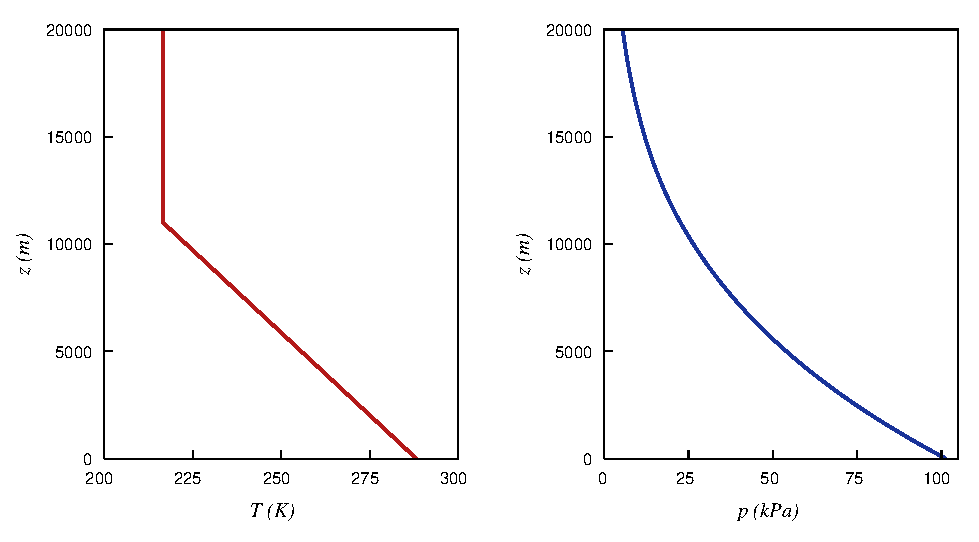
\includegraphics{../figures/FIG-0013/figure.pdf}}%
\count0=\ht0
\advance\count0 by \dp0
\count2=\wd0
\count4=\dimexpr\textheight/100*38\relax
\count6=\linewidth
\ifnum\count0<1
\count0=1
\fi
\ifnum\count2<1
\count2=1
\fi
\divide\count0 by 4096
\divide\count2 by 4096
\divide\count4 by 4096
\divide\count6 by 4096
\ifnum\count0<1
\count0=1
\fi
\ifnum\count2<1
\count2=1
\fi
\ifnum\count4<1
\count4=1
\fi
\ifnum\count6<1
\count6=1
\fi
\count8=\count2
\ifnum\count0>\count4
\count8=\numexpr\count2*\count4/\count0\relax
\fi
\ifnum\count8>\count6
\resizebox{\linewidth}{!}{\box0}%
\else
\ifnum\count0>\count4
\resizebox{!}{\dimexpr\textheight/100*38\relax}{\box0}%
\else
\box0%
\fi
\fi
\endgroup
\par\nopagebreak
\studiumcaption{fig:c05-isa}{Atmósfera estándar hasta 20 km: temperatura (izquierda, en K) y presión (derecha, en kPa) frente a la altitud. Troposfera con gradiente de 6.5 K/km hasta 11 km y capa isoterma a 216.65 K por encima.}
\end{minipage}
\par\vspace{\baselineskip}

\par\vspace{\baselineskip}
\noindent\begin{minipage}{\linewidth}
\centering
\begingroup
\setbox0=\hbox{\begin{tikzpicture}
\fill[blue!12] (-3,0) rectangle (0,3);
\draw[thick,blue] (-3,3) -- (0,3);
\fill[gray!40] (0,-0.2) rectangle (0.3,3.4);
\draw[thick] (0,0) -- (0,3);
\draw[thick] (0,3) -- (2.4,0) -- (0,0);
\foreach \y in {0.3,0.9,1.5,2.1,2.7} { \draw[->,red] (0.05,\y) -- ({2.4*(3-\y)/3},\y); }
\draw[->,ultra thick] (0.35,1.0) -- (3.2,1.0) node[pos=1.0,right]{$F$};
\draw[dashed] (-0.5,1.5) -- (0.5,1.5) node[above right]{\small centroide};
\draw[<->] (-3.4,3) -- node[left]{$H$} (-3.4,0);
\draw[<->] (2.9,3) -- node[right]{$2H/3$} (2.9,1.0);
\node at (1.5,3.3) {$p = 0$};
\node[below] at (2.4,0) {$\rho g H$};
\end{tikzpicture}}%
\count0=\ht0
\advance\count0 by \dp0
\count2=\wd0
\count4=\dimexpr\textheight/100*38\relax
\count6=\linewidth
\ifnum\count0<1
\count0=1
\fi
\ifnum\count2<1
\count2=1
\fi
\divide\count0 by 4096
\divide\count2 by 4096
\divide\count4 by 4096
\divide\count6 by 4096
\ifnum\count0<1
\count0=1
\fi
\ifnum\count2<1
\count2=1
\fi
\ifnum\count4<1
\count4=1
\fi
\ifnum\count6<1
\count6=1
\fi
\count8=\count2
\ifnum\count0>\count4
\count8=\numexpr\count2*\count4/\count0\relax
\fi
\ifnum\count8>\count6
\resizebox{\linewidth}{!}{\begin{tikzpicture}
\fill[blue!12] (-3,0) rectangle (0,3);
\draw[thick,blue] (-3,3) -- (0,3);
\fill[gray!40] (0,-0.2) rectangle (0.3,3.4);
\draw[thick] (0,0) -- (0,3);
\draw[thick] (0,3) -- (2.4,0) -- (0,0);
\foreach \y in {0.3,0.9,1.5,2.1,2.7} { \draw[->,red] (0.05,\y) -- ({2.4*(3-\y)/3},\y); }
\draw[->,ultra thick] (0.35,1.0) -- (3.2,1.0) node[pos=1.0,right]{$F$};
\draw[dashed] (-0.5,1.5) -- (0.5,1.5) node[above right]{\small centroide};
\draw[<->] (-3.4,3) -- node[left]{$H$} (-3.4,0);
\draw[<->] (2.9,3) -- node[right]{$2H/3$} (2.9,1.0);
\node at (1.5,3.3) {$p = 0$};
\node[below] at (2.4,0) {$\rho g H$};
\end{tikzpicture}}%
\else
\ifnum\count0>\count4
\resizebox{!}{\dimexpr\textheight/100*38\relax}{\begin{tikzpicture}
\fill[blue!12] (-3,0) rectangle (0,3);
\draw[thick,blue] (-3,3) -- (0,3);
\fill[gray!40] (0,-0.2) rectangle (0.3,3.4);
\draw[thick] (0,0) -- (0,3);
\draw[thick] (0,3) -- (2.4,0) -- (0,0);
\foreach \y in {0.3,0.9,1.5,2.1,2.7} { \draw[->,red] (0.05,\y) -- ({2.4*(3-\y)/3},\y); }
\draw[->,ultra thick] (0.35,1.0) -- (3.2,1.0) node[pos=1.0,right]{$F$};
\draw[dashed] (-0.5,1.5) -- (0.5,1.5) node[above right]{\small centroide};
\draw[<->] (-3.4,3) -- node[left]{$H$} (-3.4,0);
\draw[<->] (2.9,3) -- node[right]{$2H/3$} (2.9,1.0);
\node at (1.5,3.3) {$p = 0$};
\node[below] at (2.4,0) {$\rho g H$};
\end{tikzpicture}}%
\else
\begin{tikzpicture}
\fill[blue!12] (-3,0) rectangle (0,3);
\draw[thick,blue] (-3,3) -- (0,3);
\fill[gray!40] (0,-0.2) rectangle (0.3,3.4);
\draw[thick] (0,0) -- (0,3);
\draw[thick] (0,3) -- (2.4,0) -- (0,0);
\foreach \y in {0.3,0.9,1.5,2.1,2.7} { \draw[->,red] (0.05,\y) -- ({2.4*(3-\y)/3},\y); }
\draw[->,ultra thick] (0.35,1.0) -- (3.2,1.0) node[pos=1.0,right]{$F$};
\draw[dashed] (-0.5,1.5) -- (0.5,1.5) node[above right]{\small centroide};
\draw[<->] (-3.4,3) -- node[left]{$H$} (-3.4,0);
\draw[<->] (2.9,3) -- node[right]{$2H/3$} (2.9,1.0);
\node at (1.5,3.3) {$p = 0$};
\node[below] at (2.4,0) {$\rho g H$};
\end{tikzpicture}%
\fi
\fi
\endgroup
\par\nopagebreak
\studiumcaption{fig:c05-compuerta}{Distribución de presión manométrica sobre una pared vertical de altura \(H\) con el agua hasta su borde superior. La resultante \(F = \rho g b H^{2}/2\) actúa en el centro de presiones, a \(\tfrac{2H}{3}\) de profundidad, por debajo del centroide.}
\end{minipage}
\par\vspace{\baselineskip}

\par\vspace{\baselineskip}
\noindent\begin{minipage}{\linewidth}
\centering
\begingroup
\setbox0=\hbox{\begin{tikzpicture}
\draw[thick] (0,0) -- (3,0) -- (3,2) -- (0,2) -- cycle;
\draw[thick] (3,0) -- (4,0.7) -- (4,2.7) -- (3,2);
\draw[thick] (0,2) -- (1,2.7) -- (4,2.7);
\draw[dashed] (0,0) -- (1,0.7) -- (4,0.7); \draw[dashed] (1,0.7) -- (1,2.7);
\draw[->,very thick,blue] (2,-1.2) -- (2,-0.05) node[midway,right]{$p\,dx\,dy$};
\draw[->,very thick,blue] (2.5,3.9) -- (2.5,2.75) node[midway,right]{$\left(p + \frac{dp}{dz}dz\right)dx\,dy$};
\draw[->,very thick,red] (2.4,1.8) -- (2.4,1.0) node[midway,left,fill=white,inner sep=1pt]{$\rho g\,dx\,dy\,dz$};
\draw[<->] (-0.3,0) -- node[left]{$dz$} (-0.3,2);
\draw[<->] (0,-0.3) -- node[below]{$dx$} (3,-0.3);
\draw[->] (5,0) -- (5,1.4) node[above]{$z$};
\end{tikzpicture}}%
\count0=\ht0
\advance\count0 by \dp0
\count2=\wd0
\count4=\dimexpr\textheight/100*38\relax
\count6=\linewidth
\ifnum\count0<1
\count0=1
\fi
\ifnum\count2<1
\count2=1
\fi
\divide\count0 by 4096
\divide\count2 by 4096
\divide\count4 by 4096
\divide\count6 by 4096
\ifnum\count0<1
\count0=1
\fi
\ifnum\count2<1
\count2=1
\fi
\ifnum\count4<1
\count4=1
\fi
\ifnum\count6<1
\count6=1
\fi
\count8=\count2
\ifnum\count0>\count4
\count8=\numexpr\count2*\count4/\count0\relax
\fi
\ifnum\count8>\count6
\resizebox{\linewidth}{!}{\begin{tikzpicture}
\draw[thick] (0,0) -- (3,0) -- (3,2) -- (0,2) -- cycle;
\draw[thick] (3,0) -- (4,0.7) -- (4,2.7) -- (3,2);
\draw[thick] (0,2) -- (1,2.7) -- (4,2.7);
\draw[dashed] (0,0) -- (1,0.7) -- (4,0.7); \draw[dashed] (1,0.7) -- (1,2.7);
\draw[->,very thick,blue] (2,-1.2) -- (2,-0.05) node[midway,right]{$p\,dx\,dy$};
\draw[->,very thick,blue] (2.5,3.9) -- (2.5,2.75) node[midway,right]{$\left(p + \frac{dp}{dz}dz\right)dx\,dy$};
\draw[->,very thick,red] (2.4,1.8) -- (2.4,1.0) node[midway,left,fill=white,inner sep=1pt]{$\rho g\,dx\,dy\,dz$};
\draw[<->] (-0.3,0) -- node[left]{$dz$} (-0.3,2);
\draw[<->] (0,-0.3) -- node[below]{$dx$} (3,-0.3);
\draw[->] (5,0) -- (5,1.4) node[above]{$z$};
\end{tikzpicture}}%
\else
\ifnum\count0>\count4
\resizebox{!}{\dimexpr\textheight/100*38\relax}{\begin{tikzpicture}
\draw[thick] (0,0) -- (3,0) -- (3,2) -- (0,2) -- cycle;
\draw[thick] (3,0) -- (4,0.7) -- (4,2.7) -- (3,2);
\draw[thick] (0,2) -- (1,2.7) -- (4,2.7);
\draw[dashed] (0,0) -- (1,0.7) -- (4,0.7); \draw[dashed] (1,0.7) -- (1,2.7);
\draw[->,very thick,blue] (2,-1.2) -- (2,-0.05) node[midway,right]{$p\,dx\,dy$};
\draw[->,very thick,blue] (2.5,3.9) -- (2.5,2.75) node[midway,right]{$\left(p + \frac{dp}{dz}dz\right)dx\,dy$};
\draw[->,very thick,red] (2.4,1.8) -- (2.4,1.0) node[midway,left,fill=white,inner sep=1pt]{$\rho g\,dx\,dy\,dz$};
\draw[<->] (-0.3,0) -- node[left]{$dz$} (-0.3,2);
\draw[<->] (0,-0.3) -- node[below]{$dx$} (3,-0.3);
\draw[->] (5,0) -- (5,1.4) node[above]{$z$};
\end{tikzpicture}}%
\else
\begin{tikzpicture}
\draw[thick] (0,0) -- (3,0) -- (3,2) -- (0,2) -- cycle;
\draw[thick] (3,0) -- (4,0.7) -- (4,2.7) -- (3,2);
\draw[thick] (0,2) -- (1,2.7) -- (4,2.7);
\draw[dashed] (0,0) -- (1,0.7) -- (4,0.7); \draw[dashed] (1,0.7) -- (1,2.7);
\draw[->,very thick,blue] (2,-1.2) -- (2,-0.05) node[midway,right]{$p\,dx\,dy$};
\draw[->,very thick,blue] (2.5,3.9) -- (2.5,2.75) node[midway,right]{$\left(p + \frac{dp}{dz}dz\right)dx\,dy$};
\draw[->,very thick,red] (2.4,1.8) -- (2.4,1.0) node[midway,left,fill=white,inner sep=1pt]{$\rho g\,dx\,dy\,dz$};
\draw[<->] (-0.3,0) -- node[left]{$dz$} (-0.3,2);
\draw[<->] (0,-0.3) -- node[below]{$dx$} (3,-0.3);
\draw[->] (5,0) -- (5,1.4) node[above]{$z$};
\end{tikzpicture}%
\fi
\fi
\endgroup
\par\nopagebreak
\studiumcaption{fig:c05-elemento}{Equilibrio vertical de un paralelepípedo elemental de fluido en reposo: la diferencia entre las fuerzas de presión sobre las caras inferior y superior equilibra el peso \(\rho g\,dx\,dy\,dz\).}
\end{minipage}
\par\vspace{\baselineskip}

Si la densidad es uniforme, como en un líquido, la integración de \(dp/dz = -\rho g\) entre la superficie libre, a cota \(z_0\) y presión \(p_0\), y un punto a cota \(z\) da \(p = p_0 - \rho g\,(z - z_0)\), que escrita con la profundidad \(h = z_0 - z\) es la ecuación fundamental de la hidrostática,
\begin{equation}
p = p_0 + \rho g h. \label{eq:c05-hidrostatica}
\end{equation}
En agua, la presión aumenta unos \(9.81\) kPa por cada metro de profundidad, casi una atmósfera cada diez metros. Una consecuencia inmediata es el principio de Pascal: cualquier variación de la presión en la superficie se transmite íntegramente a todos los puntos del líquido, porque solo cambia la constante \(p_0\). En ello se basan la prensa hidráulica y los sistemas hidráulicos de mando de una aeronave: una fuerza \(F_1\) aplicada sobre un émbolo de área \(A_1\) genera una presión \(F_1/A_1\) que actúa sobre un émbolo de área \(A_2\) y produce una fuerza \(F_2 = F_1 A_2/A_1\), a costa de que el émbolo grande se desplace una distancia menor en la misma proporción. La ecuación \(\eqref{eq:c05-general}\) es más general que \(\eqref{eq:c05-hidrostatica}\): si el fluido gira como un sólido rígido con velocidad angular \(\Omega\), en ejes que giran con él se añade la fuerza centrífuga por unidad de volumen \(\rho\Omega^{2}r\), la presión pasa a ser \(p = p_0 + \tfrac12\rho\Omega^{2}r^{2} - \rho g(z - z_0)\) y la superficie libre, donde la presión es la atmosférica, es el paraboloide \(z_s = z_0 + \Omega^{2}r^{2}/(2g)\). El mismo razonamiento explica la inclinación de la superficie del combustible en un depósito que acelera horizontalmente, un problema de diseño real de los sistemas de combustible.

\section{Medida de presiones}

La presión puede medirse respecto al vacío absoluto o respecto a la presión atmosférica local. La presión absoluta es la que aparece en la ecuación de estado y en las ecuaciones de la mecánica de fluidos; la presión manométrica es la diferencia entre la absoluta y la atmosférica, y es la que indican la mayoría de los manómetros, como el de los neumáticos. Una presión manométrica negativa se denomina depresión o vacío parcial. Confundir ambas referencias es un error clásico: un neumático de avión inflado a 1.0 MPa manométricos contiene aire a unos 1.1 MPa absolutos, y es esta última la presión que debe usarse en la ecuación de estado. El barómetro de mercurio de Torricelli mide la presión atmosférica absoluta: en un tubo cerrado por arriba e invertido sobre una cubeta, el mercurio desciende hasta que el peso de la columna equilibra la presión atmosférica, dejando vacío en la parte superior. Con una densidad del mercurio de \(13\,595.1\) kg/m\(^3\) y la gravedad estándar, una columna de 760 mm equivale a \(13\,595.1\cdot 9.80665\cdot 0.760 \approx 1.0133\times 10^{5}\) Pa, la atmósfera estándar. De ahí proceden las unidades manométricas como el milímetro de mercurio o el centímetro de agua.

El manómetro de tubo en U mide diferencias de presión mediante una columna de líquido. Si una rama está conectada a un recipiente con presión \(p_a\) y la otra está abierta a la atmósfera, el líquido manométrico de densidad \(\rho_m\) se desnivela una altura \(h\) tal que \(p_a - p_{atm} = \rho_m g h\), siempre que el fluido del recipiente sea un gas de densidad despreciable. Cuando hay varios fluidos, la regla práctica consiste en recorrer el manómetro desde un extremo hasta el otro sumando \(\rho g\,\Delta h\) al descender y restándolo al ascender en cada fluido, teniendo en cuenta que solo pueden igualarse las presiones de dos puntos a la misma cota si están unidos por el mismo fluido continuo en reposo. Para medir diferencias pequeñas, como las que se dan en un túnel aerodinámico de baja velocidad, se usa un líquido ligero y se inclina la rama de lectura un ángulo \(\theta\) respecto a la horizontal: la longitud leída \(L\) a lo largo del tubo corresponde a un desnivel vertical \(h = L\sin\theta\), de modo que la sensibilidad se multiplica por \(1/\sin\theta\). Para diferencias grandes se usa mercurio, cuya densidad mantiene la columna dentro de una longitud manejable. Los transductores electrónicos han sustituido en la práctica a los manómetros de líquido, pero estos siguen siendo el patrón primario de calibración en muchos laboratorios precisamente porque su principio de medida se reduce a la ecuación \(\eqref{eq:c05-hidrostatica}\).

\section{Fuerzas sobre superficies y flotación}

La fuerza que un líquido en reposo ejerce sobre una superficie plana sumergida es la integral de la presión sobre ella. Si la presión atmosférica actúa por ambas caras de la superficie, como en una compuerta o en la pared de un depósito abierto, basta con integrar la presión manométrica \(\rho g h\). Para una superficie plana de área \(A\) cuyo centroide está a una profundidad \(h_c\), la integral se reduce a
\begin{equation}
F = \int_A \rho g h\,dA = \rho g\,h_c\,A, \label{eq:c05-fuerza}
\end{equation}
es decir, al producto de la presión en el centroide por el área. La fuerza es perpendicular a la superficie, pero no se aplica en el centroide sino en el centro de presiones, más profundo, porque la presión crece con la profundidad. Igualando el momento de la resultante respecto a la línea de la superficie libre con el momento de la distribución, y aplicando el teorema de Steiner, se obtiene para una superficie vertical \(h_{cp} = h_c + I_{xc}/(h_c A)\), donde \(I_{xc}\) es el momento de inercia del área respecto a un eje horizontal que pasa por su centroide. Para un rectángulo vertical de altura \(H\) y anchura \(b\) cuyo borde superior está en la superficie, el centroide está a la profundidad \(H/2\), \(I_{xc} = bH^{3}/12\) y el centro de presiones queda a \(\tfrac{2H}{3}\) de profundidad, el centroide del triángulo de presiones; es el caso de una presa de paramento vertical, en la que la fuerza total por unidad de anchura vale \(\rho g H^{2}/2\). La figura~\ref{fig:c05-compuerta} muestra la distribución triangular y la posición de la resultante. Para superficies curvas se calculan por separado la componente horizontal, igual a la fuerza sobre la proyección vertical de la superficie, y la componente vertical, igual al peso del líquido situado sobre ella.

El principio de Arquímedes es una consecuencia directa de la ecuación de la hidrostática. Sobre un cuerpo sumergido, las fuerzas horizontales de presión se cancelan, mientras que la presión sobre las caras inferiores es mayor que sobre las superiores. Para un paralelepípedo elemental de caras horizontales, la diferencia de presiones multiplicada por el área de la cara es igual al peso del fluido que ocuparía su volumen; sumando una infinidad de paralelepípedos el resultado se extiende a un cuerpo de forma arbitraria: un cuerpo sumergido total o parcialmente en un fluido en reposo experimenta un empuje vertical y ascendente igual al peso del fluido desalojado, \(E = \rho_f g V_{\mathrm{sum}}\), aplicado en el centroide del volumen desalojado, llamado centro de carena. El empuje no depende de la profundidad si el fluido es incompresible, ni del material del cuerpo. Un cuerpo flota en equilibrio cuando el empuje iguala a su peso; la estabilidad de ese equilibrio depende de la posición relativa del centro de gravedad y del metacentro, y se cuantifica con la altura metacéntrica, que debe ser positiva para que el cuerpo recupere su posición al escorarse. En el aire el principio rige el vuelo de globos y dirigibles: un globo de aire caliente sustenta la diferencia entre el peso del aire frío desalojado y el del aire caliente que contiene.

\section{La atmósfera estándar}

En un gas la densidad no es constante, y la ecuación \(\eqref{eq:c05-general}\) debe integrarse junto con la ecuación de estado. Sustituyendo \(\rho = p/(R_a T)\) en \(dp/dz = -\rho g\) se obtiene \(dp/p = -g\,dz/(R_a T)\), que solo puede integrarse si se conoce la distribución de temperatura con la altitud. En una capa isoterma,
\begin{equation}
p = p_0\,\exp\!\left(-\frac{g z}{R_a T}\right) = p_0\,e^{-z/H_e}, \qquad H_e = \frac{R_a T}{g}, \label{eq:c05-isoterma}
\end{equation}
y la presión decrece exponencialmente con una altura de escala \(H_e\); para \(T = 288.15\) K, la altura de escala vale \(287.05\cdot 288.15/9.80665 \approx 8434\) m. La baja estratosfera, entre 11 y 20 km, es casi isoterma a \(216.65\) K, y en ella la presión decrece según esta ley: partiendo de unos \(22\,632\) Pa a 11 km, la ecuación \(\eqref{eq:c05-isoterma}\) da a 20 km \(22\,632\exp[-9.80665\cdot 9000/(287.05\cdot 216.65)] \approx 5.475\times 10^{3}\) Pa, apenas una vigésima parte de la presión a nivel del mar.

En la troposfera, hasta 11 km, la atmósfera estándar supone que la temperatura disminuye linealmente con la altitud, \(T = T_0 - \Gamma z\), con \(T_0\) igual a 288.15 K y un gradiente \(\Gamma = 0.0065\) K/m. Integrando \(dp/p = -g\,dz/[R_a(T_0 - \Gamma z)]\) resulta
\begin{equation}
p = p_0\left(1 - \frac{\Gamma z}{T_0}\right)^{g/(R_a\Gamma)}, \label{eq:c05-troposfera}
\end{equation}
con un exponente \(g/(R_a\Gamma) = 9.80665/(287.05\cdot 0.0065) \approx 5.256\), el mismo que aparece en el ajuste empírico que publica la NASA para la troposfera. En la tropopausa, donde la temperatura ha descendido a \(216.65\) K, la presión vale \(101\,325\,(216.65/288.15)^{5.256} \approx 2.263\times 10^{4}\) Pa, en buen acuerdo con el valor tabulado. La densidad se obtiene después de la ecuación de estado. La figura~\ref{fig:c05-isa} representa la temperatura y la presión de este modelo hasta 20 km. Conviene recordar que la atmósfera estándar es una convención de ingeniería, no una descripción de la atmósfera real en un día concreto: sirve para comparar actuaciones de aeronaves, calibrar altímetros, que en realidad son barómetros graduados en metros según la ecuación \(\eqref{eq:c05-troposfera}\), y definir condiciones de referencia para los ensayos. La atmósfera real se aparta de ella con la latitud, la estación y la situación meteorológica, y por eso los pilotos ajustan el altímetro con la presión local.

\begin{tcolorbox}[title={Consejo}, studiumtip, breakable]

En los manómetros de varios fluidos, escriba la cadena de presiones desde un extremo al otro sin saltar de fluido; solo dos puntos a la misma altura en el mismo fluido continuo tienen la misma presión. Y antes de usar una presión en la ecuación de estado, compruebe que es absoluta.
\end{tcolorbox}

\begin{tcolorbox}[title={Definición}, studiumdef, breakable]

Presión: fuerza normal de compresión por unidad de superficie que el fluido ejerce sobre cualquier superficie en contacto con él. En un fluido en reposo es un escalar, la misma en todas las direcciones en cada punto, y se mide en pascales (newtons por metro cuadrado).
\end{tcolorbox}



% Revision bibliografica 2026: material original, contrastes verificables.

\section{Contraste bibliográfico: fuerza hidrostática y centro de presiones}
\label{sec:ref26-hidro}

La presión de un fluido homogéneo en reposo, medida respecto de la presión que actúa al otro lado de la superficie, es \(p_{\mathrm{man}}(h)=\rho gh\) para profundidad vertical \(h\) medida desde la superficie libre. Se supone densidad constante, gravedad uniforme y superficie libre con presión de referencia uniforme. No debe confundirse la presión manométrica con la absoluta: si ambas caras de una compuerta están sometidas a la misma presión atmosférica, esa contribución se cancela en la fuerza neta.

En una placa \emph{vertical}, rectangular, de anchura \(b\), altura \(H\) y borde superior a profundidad \(h_0\), la fuerza y su punto de aplicación se obtienen integrando la distribución, no evaluando la presión máxima:
\begin{equation}
 F=\int_0^H \rho g(h_0+y)b\,dy
   =\rho g A h_c,\quad
 A=bH,\quad h_c=h_0+\frac{H}{2}.
 \label{eq:ref26-hidro-fuerza}
\end{equation}
Al igualar momentos respecto a la superficie libre,
\begin{equation}
 h_{\mathrm{cp}}
 =\frac{\int_A h^2\,dA}{\int_A h\,dA}
 =h_c+\frac{I_G}{Ah_c},\qquad I_G=\frac{bH^3}{12},
 \label{eq:ref26-hidro-cp}
\end{equation}
donde \(I_G\) es el segundo momento del área respecto del eje \emph{horizontal centroidal}. La segunda expresión presupone una superficie plana vertical; para una placa inclinada debe introducirse el ángulo geométrico correspondiente. El centro de presiones queda por debajo del centroide si la superficie está totalmente sumergida.

\begin{tcolorbox}[title={Ejemplo guiado original: compuerta}, studiumdef, breakable]
Una compuerta vertical de \(1{,}20\,\mathrm{m}\) de anchura y \(1{,}50\,\mathrm{m}\) de altura tiene el borde superior a \(0{,}60\,\mathrm{m}\) de profundidad. Para agua con \(\rho=1000\,\mathrm{kg\,m^{-3}}\) y \(g=9{,}81\,\mathrm{m\,s^{-2}}\), se obtiene \(A=1{,}80\,\mathrm{m^2}\), \(h_c=1{,}35\,\mathrm{m}\) y \(I_G=0{,}3375\,\mathrm{m^4}\).
La resultante vale \(F=1000\cdot9{,}81\cdot1{,}80\cdot1{,}35=\mathbf{23838{,}3\,\mathrm{N}}\).
La profundidad de su línea de acción es
\[
 h_{\mathrm{cp}}=1{,}35+\frac{0{,}3375}{1{,}80\cdot1{,}35}
 =\mathbf{1{,}48889\,\mathrm{m}},
\]
es decir, \(0{,}88889\,\mathrm{m}\) por debajo del borde superior. Se verifica \(h_c<h_{\mathrm{cp}}<h_0+H\), como exige la distribución triangular/trapezoidal de presiones. Las unidades de \(I_G/(Ah_c)\) son metros.
\end{tcolorbox}

\textbf{Autocomprobación.} ¿Qué ocurre si el borde superior coincide con la superficie libre (\(h_0=0\))? Demuestre que \(h_{\mathrm{cp}}=2H/3\) y no \(H/2\). Explique por qué una misma presión atmosférica sobre ambas caras no cambia el resultado. La deducción es propia; el tratamiento general de las distribuciones de presión se contrasta con White, capítulo 2 \cite{ref26-white}.


\section{Desarrollos y práctica}

Las deducciones que siguen parten de la ecuación fundamental de la hidrostática \(\eqref{eq:c05-general}\) y la integran en los casos que aparecen en ingeniería aeroespacial: el líquido de densidad constante \(\eqref{eq:c05-hidrostatica}\), incluida la superficie libre de un líquido en rotación; la fuerza y el centro de presiones sobre una compuerta \(\eqref{eq:c05-fuerza}\); y la atmósfera, primero isoterma \(\eqref{eq:c05-isoterma}\) y después con gradiente térmico constante \(\eqref{eq:c05-troposfera}\), que es el modelo de la troposfera estándar. En los ejercicios es esencial distinguir entre presión absoluta y manométrica y, en los gases, recordar que la densidad varía con la altura.

\begin{tcolorbox}[title={Desarrollos del modelo}, studiumdef, breakable]

\noindent\textbf{Ecuación fundamental de la hidrostática}

\[
p = p_0 + \rho g h
\]

\noindent\textbf{Hipótesis}
\begin{itemize}
\item fluido en reposo en un sistema inercial
\item densidad y gravedad uniformes
\item h medida hacia abajo desde la superficie libre
\end{itemize}

\noindent\textbf{Limitaciones}
\begin{itemize}
\item no vale si la densidad varía apreciablemente (gases en grandes alturas)
\end{itemize}

\noindent\textbf{Pasos}
\begin{enumerate}
\item
equilibrio de un elemento: el gradiente de presión equilibra el peso

\[
\nabla p = \rho\,\mathbf{g},\qquad \frac{dp}{dz} = -\rho g
\]
\item
integrar en z con densidad constante

\[
p(z) = p_0 - \rho g\,(z - z_0)
\]
\item
sustituir la cota por la profundidad h = z0 - z

\[
p = p_0 + \rho g h
\]
\item
relación usada en el texto (paso intermedio no comprobado por separado)

\[
dp/dz = -\rho g
\]
\end{enumerate}

\noindent\textbf{Variables}
\begin{itemize}
\item $h$: profundidad ($\mathrm{m}$)
\end{itemize}



\noindent\textbf{Superficie libre de un líquido en rotación como sólido rígido}

\begin{equation}
z_s(r) = z_0 + \frac{\Omega^{2} r^{2}}{2g}
\label{eq:c05-paraboloide}
\end{equation}

\noindent\textbf{Hipótesis}
\begin{itemize}
\item líquido que gira con velocidad angular constante como un sólido rígido
\item densidad uniforme
\end{itemize}

\noindent\textbf{Limitaciones}
\begin{itemize}
\item se alcanza solo tras el transitorio de arranque, cuando la viscosidad ha impuesto la rotación rígida
\end{itemize}

\noindent\textbf{Pasos}
\begin{enumerate}
\item
en ejes que giran con el recipiente el líquido está en reposo bajo la gravedad y la fuerza centrífuga

\[
\frac{\partial p}{\partial r} = \rho\,\Omega^{2} r,\qquad \frac{\partial p}{\partial z} = -\rho g
\]
\item
integrar el equilibrio en r y en z

\[
p = p_0 + \tfrac12\rho\,\Omega^{2} r^{2} - \rho g\,(z - z_0)
\]
\item
imponer presión atmosférica en la superficie libre

\[
z_s = z_0 + \frac{\Omega^{2} r^{2}}{2g}
\]
\end{enumerate}

\noindent\textbf{Variables}
\begin{itemize}
\item $z_{0}$: cota del vértice de la superficie libre ($\mathrm{m}$)
\end{itemize}



\noindent\textbf{Fuerza y centro de presiones sobre una superficie plana vertical rectangular}

\begin{equation}
F = \rho g\,h_c\,A,\qquad h_{cp} = h_c + \frac{I_{xc}}{h_c A}
\label{eq:c05-superficie}
\end{equation}

\noindent\textbf{Hipótesis}
\begin{itemize}
\item superficie plana vertical sumergida en un líquido de densidad uniforme
\item presión manométrica (la atmosférica actúa por ambas caras)
\end{itemize}

\noindent\textbf{Limitaciones}
\begin{itemize}
\item para un plano inclinado un ángulo \(\theta\) respecto a la horizontal y cuya profundidad \(h_c\) se mide verticalmente, \(h_{cp}=h_c+I_G\sin^2\theta/(h_c A)\), con \(I_G\) respecto al eje centroidal paralelo a la intersección del plano con la superficie libre; si se usan distancias \(s\) medidas a lo largo del plano, \(s_{cp}=s_c+I_G/(s_c A)\). Estas fórmulas suponen densidad uniforme y presión manométrica hidrostática.
\end{itemize}

\noindent\textbf{Pasos}
\begin{enumerate}
\item
integrar la presión rho g h sobre el área

\[
F = \int_A \rho g h\,dA = \rho g\,h_c A
\]
\item
igualar el momento de la resultante al momento de la distribución

\[
F\,h_{cp} = \int_A \rho g h^{2}\,dA = \rho g\left(I_{xc} + h_c^{2} A\right)
\]
\item
para un rectángulo de altura H con el borde superior en la superficie, \(h_cp = 2H/3\)

\[
h_{cp} = \frac{2H}{3}\quad(\text{rectángulo desde la superficie})
\]
\end{enumerate}

\noindent\textbf{Variables}
\begin{itemize}
\item $A$: área de la superficie ($\mathrm{m}^{2}$)
\end{itemize}



\noindent\textbf{Presión en una atmósfera isoterma}

\[
p = p_0\,\exp\!\left(-\frac{g z}{R_a T}\right) = p_0\,e^{-z/H_e},\qquad H_e = \frac{R_a T}{g}
\]

\noindent\textbf{Hipótesis}
\begin{itemize}
\item gas ideal
\item temperatura uniforme
\item gravedad uniforme
\end{itemize}

\noindent\textbf{Limitaciones}
\begin{itemize}
\item describe bien la baja estratosfera (11 a 20 km), donde la temperatura es casi constante
\end{itemize}

\noindent\textbf{Pasos}
\begin{enumerate}
\item
combinar el equilibrio hidrostático con la ecuación de estado

\[
\frac{dp}{dz} = -\rho g = -\frac{p\,g}{R_a T}
\]
\item
separar variables e integrar

\[
\ln\frac{p}{p_0} = -\frac{g z}{R_a T}
\]
\item
relación usada en el texto (paso intermedio no comprobado por separado)

\[
\rho = p/(R_a T)
\]
\item
relación usada en el texto (paso intermedio no comprobado por separado)

\[
dp/p = -g\,dz/(R_a T)
\]
\end{enumerate}

\noindent\textbf{Variables}
\begin{itemize}
\item $H_{e}$: altura de escala ($\mathrm{m}$)
\end{itemize}



\noindent\textbf{Presión en una troposfera con gradiente térmico constante}

\[
T = T_0 - \Gamma z,\qquad p = p_0\left(1 - \frac{\Gamma z}{T_0}\right)^{g/(R_a\Gamma)}
\]

\noindent\textbf{Hipótesis}
\begin{itemize}
\item gas ideal
\item temperatura lineal con la altitud
\item gravedad uniforme
\end{itemize}

\noindent\textbf{Limitaciones}
\begin{itemize}
\item la atmósfera real se aparta del modelo según la latitud, la estación y el tiempo atmosférico
\end{itemize}

\noindent\textbf{Pasos}
\begin{enumerate}
\item
sustituir T = T0 - Gamma z en \(dp/p = -g dz/(R_a T)\)

\[
\frac{dp}{p} = -\frac{g\,dz}{R_a\,(T_0 - \Gamma z)}
\]
\item
integrar entre el nivel del mar y z

\[
\ln\frac{p}{p_0} = \frac{g}{R_a\Gamma}\ln\frac{T_0 - \Gamma z}{T_0}
\]
\end{enumerate}

\noindent\textbf{Variables}
\begin{itemize}
\item $\Gamma$: gradiente térmico (0.0065 K/m en la atmósfera estándar) ($\mathrm{K}\,\mathrm{m}^{-1}$)
\end{itemize}


\end{tcolorbox}

\begin{tcolorbox}[title={Problema resuelto}, studiumworked, breakable]

\noindent\textbf{Enunciado}
La pared vertical de un tanque de ensayos hidrodinámicos tiene una ventana de observación rectangular de \(2.0\) m de anchura y \(3.0\) m de altura cuyo borde superior está \(1.0\) m por debajo de la superficie libre del agua (\(\rho = 1000\) kg/m\(^3\), \(g = 9.81\) m/s\(^2\)). La otra cara de la ventana está a presión atmosférica. Calcule la fuerza hidrostática sobre la ventana y la profundidad de su centro de presiones.

\noindent\textbf{Datos}
\begin{itemize}
\item $\rho = 1000\,\mathrm{kg}\,\mathrm{m}^{-3}$ — densidad del agua
\item $g = 9.81\,\mathrm{m}\,\mathrm{s}^{-2}$ — gravedad
\item $b = 2.0\,\mathrm{m}$ — anchura
\item $H = 3.0\,\mathrm{m}$ — altura
\item $h_{t} = 1.0\,\mathrm{m}$ — profundidad del borde superior
\end{itemize}

\noindent\textbf{Incógnita}
profundidad del centro de presiones

\noindent\textbf{Modelo físico}

\noindent\textit{Centro de presiones de un rectángulo vertical}

\[
h_{cp} = h_c + \frac{H^{2}}{12\,h_c},\quad h_c = h_t + \frac{H}{2}
\]

\noindent\textbf{Hipótesis}
\begin{itemize}
\item agua en reposo y de densidad uniforme
\item la presión atmosférica actúa por ambas caras y se cancela
\end{itemize}

\noindent\textbf{Desarrollo paso a paso}

\phantomsection\label{solution:mf-005}
\noindent\textbf{Elección del procedimiento.} La presión manométrica es $p(h)=\rho gh$. La fuerza es la integral de esa presión, y la posición se obtiene igualando momentos: $Fh_{cp}=\int h\,p\,dA$. Para el rectángulo, $h_c=h_t+H/2$ e $I_G=bH^3/12$.

\begin{enumerate}

\item El centroide está a media altura bajo el borde superior.

\[\fitmath{\mathrm{hc}=\mathrm{ht}+\frac{H}{2}}\]

\[\fitmath{\mathrm{hc}=(1)+\frac{(3)}{2}\approx 2.5\,\mathrm{m}}\]

\item Calcular el área sobre la que actúa la presión.

\[\fitmath{A=b\cdot H}\]

\[\fitmath{A=(2)\cdot (3)\approx 6\,\mathrm{m^{2}}}\]

\item La integral de una presión lineal equivale a la presión en el centroide por el área.

\[\fitmath{F=\rho\cdot g\cdot \mathrm{hc}\cdot A}\]

\[\fitmath{F=(1000)\cdot (9.81)\cdot (2.5)\cdot (6)\approx 147150\,\mathrm{N}}\]

\item La integral del momento requiere la inercia geométrica respecto al eje centroidal horizontal.

\[\fitmath{\mathrm{IG}=\frac{b\cdot {H}^{3}}{12}}\]

\[\fitmath{\mathrm{IG}=\frac{(2)\cdot {(3)}^{3}}{12}\approx 4.5\,\mathrm{m^{4}}}\]

\item De $Fh_{cp}=\rho g(I_G+Ah_c^2)$ se despeja la profundidad de aplicación.

\[\fitmath{\mathrm{hcp}=\mathrm{hc}+\frac{\mathrm{IG}}{\mathrm{hc}\cdot A}}\]

\[\fitmath{\mathrm{hcp}=(2.5)+\frac{(4.5)}{(2.5)\cdot (6)}\approx 2.8\,\mathrm{m}}\]

\end{enumerate}


\noindent\textbf{Sustitución numérica}

\[
\frac{\left(3.0\,\mathrm{m}\right)^{2}}{6 \left(3.0\,\mathrm{m}\right) + 12 \left(1.0\,\mathrm{m}\right)} + \frac{\left(3.0\,\mathrm{m}\right)}{2} + \left(1.0\,\mathrm{m}\right)
\]

\noindent\textbf{Resultado}

\[
F \approx 1.47\times 10^{5}\ \mathrm{N},\qquad h_{cp} = 2.80\ \mathrm{m}
\]

\noindent\textbf{Interpretación}
El centro de presiones está 0.30 m por debajo del centroide; la diferencia disminuiría si la ventana estuviera más profunda, porque la distribución de presiones se haría más uniforme.

\noindent\textbf{Comprobación de la respuesta} la aritmética del último paso reproduce la respuesta enunciada a la precisión con que está escrita. Es una reproducción aritmética; no valida el modelo físico ni sus hipótesis.

\noindent\textbf{Limitaciones}
\begin{itemize}
\item no incluye la presión dinámica si el agua del tanque está en movimiento
\end{itemize}

\noindent\textbf{Errores frecuentes}
\begin{itemize}
\item aplicar la fuerza en el centroide
\item usar la profundidad del borde superior en lugar de la del centroide
\end{itemize}
\end{tcolorbox}

\begin{tcolorbox}[title={Ejercicios propuestos}, studiumworked, breakable]

\noindent\textbf{1 (Básico, Cálculo)}
Calcule la presión manométrica en el fondo de un depósito de agua de 10 m de profundidad (\(\rho = 1000\) kg/m\(^3\), \(g = 9.81\) m/s\(^2\)) y exprésela en atmósferas estándar.

\noindent\textbf{2 (Básico, Cálculo)}
Un manómetro de agua (\(\rho = 998\) kg/m\(^3\)) conectado a la cámara de remanso de un túnel aerodinámico marca un desnivel de 150 mm respecto a la atmósfera. ¿Cuál es la sobrepresión en la cámara? Desprecie la densidad del aire.

\noindent\textbf{3 (Intermedio, DESIGN)}
Un micromanómetro inclinado usa alcohol de densidad 790 kg/m\(^3\) y su rama de lectura forma \(15^\circ\) con la horizontal. Si la lectura a lo largo del tubo es de 120 mm, ¿qué diferencia de presión mide? ¿Por qué factor se ha multiplicado la sensibilidad respecto a un tubo vertical?

\noindent\textbf{4 (Intermedio, Aplicación)}
Un recipiente cilíndrico con agua gira alrededor de su eje vertical como un sólido rígido. ¿A qué velocidad angular la superficie libre a \(r = 0.20\) m está \(0.10\) m por encima del vértice del paraboloide? (\(g = 9.81\) m/s\(^2\))

\noindent\textbf{5 (Avanzado, Desarrollo)}
Un globo de aire caliente tiene un volumen de 2800 m\(^3\). El aire exterior está a 15 \(^\circ\)C y \(101\,325\) Pa, y el interior a 100 \(^\circ\)C a la misma presión. Con \(R_a = 287.05\) J/(kg K), calcule la masa máxima (envoltura, cesta, quemadores y pasajeros) que puede sustentar el globo.

\noindent\textbf{6 (De examen, COMPARATIVE)}
Calcule la presión de la atmósfera estándar a 8000 m con el modelo de gradiente térmico constante (\(T_0 = 288.15\) K, \(\Gamma = 0.0065\) K/m, \(p_0 = 101\,325\) Pa, \(R_a = 287.05\) J/(kg K), \(g = 9.80665\) m/s\(^2\)) y compárela con la que se obtendría suponiendo, erróneamente, una atmósfera isoterma a 288.15 K.
\end{tcolorbox}

\begin{tcolorbox}[title={Autoevaluación}, studiumcheck, breakable]

(1) Demuestre que en un fluido en reposo la presión no varía en un plano horizontal. (2) ¿Por qué la fuerza sobre una compuerta vertical no se aplica en su centroide? (3) Un cubo de hielo flota en un vaso lleno hasta el borde: ¿se derrama el agua al fundirse? (4) ¿Qué ocurre con el empuje sobre un submarino al descender si el agua se considera incompresible? ¿Y si se tiene en cuenta su ligera compresibilidad? (5) Explique por qué un altímetro barométrico marca una altitud distinta de la real un día de bajas presiones. (6) ¿Por qué no puede integrarse la ecuación de la hidrostática en la atmósfera sin conocer la temperatura?
\end{tcolorbox}
\studiumchaptercheck

\chapter{Flujos internos laminares: Couette y Poiseuille}
\label{chap:c06}

\studiumchapterguide{Los flujos laminares entre placas y en tubos son de los pocos casos en que las ecuaciones del movimiento de un fluido viscoso tienen solución exacta. La guía docente los incluye entre los casos de estudio con nombre propio: flujos de Couette y de Poiseuille. Este capítulo los obtiene a partir de un balance de fuerzas sobre una lámina de fluido, sin necesidad todavía de las ecuaciones de Navier-Stokes, con las que se recuperarán en el capítulo 14 como soluciones exactas. Los resultados tienen aplicación directa en lubricación, en las fugas a través de holguras de válvulas hidráulicas, en los viscosímetros y en el diseño de conductos de pequeño diámetro, y proporcionan además la referencia laminar con la que se compararán los flujos turbulentos.}

\section{Flujo de Couette}

Consideremos un fluido newtoniano entre dos placas planas, paralelas e indefinidas separadas una distancia \(h\); la placa inferior está fija y la superior se mueve en su propio plano con velocidad \(U\) en la dirección \(x\). Buscamos una solución estacionaria y unidireccional, \(\mathbf{u} = (u(y), 0, 0)\), en la que el perfil de velocidad es el mismo en todas las secciones: un flujo completamente desarrollado. Para un fluido incompresible esa forma satisface automáticamente la conservación de la masa, porque el caudal que entra en una sección sale por la siguiente. Como la velocidad de cada partícula es constante a lo largo de su trayectoria rectilínea, su aceleración es nula y las fuerzas sobre cualquier porción de fluido deben equilibrarse. Tomemos una lámina de espesor \(dy\) y longitud \(dx\) por unidad de anchura. En la dirección \(x\) actúan la presión sobre las caras verticales y el esfuerzo cortante sobre las horizontales: \([p(x) - p(x + dx)]\,dy + [\tau(y + dy) - \tau(y)]\,dx = 0\), es decir,
\begin{equation}
\frac{d\tau}{dy} = \frac{dp}{dx}. \label{eq:c06-balance}
\end{equation}
Si no se impone ningún gradiente de presión, el esfuerzo es uniforme y, con la ley de Newton, \(\mu\,d^{2}u/dy^{2} = 0\). Las condiciones de no deslizamiento, \(u(0) = 0\) y \(u(h) = U\), dan el perfil lineal \(u = Uy/h\) ya encontrado en el capítulo 3, con un esfuerzo cortante \(\mu U/h\) en toda la holgura y un caudal por unidad de anchura \(q = Uh/2\). Es el flujo de Couette, base del cálculo de cojinetes poco cargados y de los viscosímetros rotativos.

\par\vspace{\baselineskip}
\noindent\begin{minipage}{\linewidth}
\centering
\begingroup
\setbox0=\hbox{\begin{tikzpicture}
\fill[gray!35] (0,1.5) rectangle (6,1.7); \fill[gray!35] (0,-1.5) rectangle (6,-1.7);
\draw[thick] (0,1.5) -- (6,1.5); \draw[thick] (0,-1.5) -- (6,-1.5);
\draw[dashdotted] (-0.3,0) -- (6.3,0);
\draw[thick,blue,domain=-1.5:1.5,samples=40] plot ({1+1.6*(1-(\x/1.5)^2)},\x);
\foreach \y in {-1.2,-0.8,-0.4,0,0.4,0.8,1.2} { \draw[->,blue] (1,\y) -- ({1+1.6*(1-(\y/1.5)^2)},\y); }
\draw (1,-1.5) -- (1,1.5);
\draw[thick,red] (3.6,-0.7) rectangle (5.4,0.7);
\draw[->,red] (3.1,0) -- (3.6,0) node[pos=0,left]{\scriptsize $p_1$};
\draw[->,red] (5.9,0) -- (5.4,0) node[pos=0,right]{\scriptsize $p_2$};
\draw[<-,red] (3.8,0.85) -- (5.2,0.85) node[midway,above]{\scriptsize $\tau$};
\draw[<->] (6.5,0) -- node[right]{$R$} (6.5,1.5);
\draw[<->] (5.6,0) -- node[right]{\scriptsize $r$} (5.6,0.7);
\node at (1.9,1.15) {$u(r)$};
\end{tikzpicture}}%
\count0=\ht0
\advance\count0 by \dp0
\count2=\wd0
\count4=\dimexpr\textheight/100*38\relax
\count6=\linewidth
\ifnum\count0<1
\count0=1
\fi
\ifnum\count2<1
\count2=1
\fi
\divide\count0 by 4096
\divide\count2 by 4096
\divide\count4 by 4096
\divide\count6 by 4096
\ifnum\count0<1
\count0=1
\fi
\ifnum\count2<1
\count2=1
\fi
\ifnum\count4<1
\count4=1
\fi
\ifnum\count6<1
\count6=1
\fi
\count8=\count2
\ifnum\count0>\count4
\count8=\numexpr\count2*\count4/\count0\relax
\fi
\ifnum\count8>\count6
\resizebox{\linewidth}{!}{\begin{tikzpicture}
\fill[gray!35] (0,1.5) rectangle (6,1.7); \fill[gray!35] (0,-1.5) rectangle (6,-1.7);
\draw[thick] (0,1.5) -- (6,1.5); \draw[thick] (0,-1.5) -- (6,-1.5);
\draw[dashdotted] (-0.3,0) -- (6.3,0);
\draw[thick,blue,domain=-1.5:1.5,samples=40] plot ({1+1.6*(1-(\x/1.5)^2)},\x);
\foreach \y in {-1.2,-0.8,-0.4,0,0.4,0.8,1.2} { \draw[->,blue] (1,\y) -- ({1+1.6*(1-(\y/1.5)^2)},\y); }
\draw (1,-1.5) -- (1,1.5);
\draw[thick,red] (3.6,-0.7) rectangle (5.4,0.7);
\draw[->,red] (3.1,0) -- (3.6,0) node[pos=0,left]{\scriptsize $p_1$};
\draw[->,red] (5.9,0) -- (5.4,0) node[pos=0,right]{\scriptsize $p_2$};
\draw[<-,red] (3.8,0.85) -- (5.2,0.85) node[midway,above]{\scriptsize $\tau$};
\draw[<->] (6.5,0) -- node[right]{$R$} (6.5,1.5);
\draw[<->] (5.6,0) -- node[right]{\scriptsize $r$} (5.6,0.7);
\node at (1.9,1.15) {$u(r)$};
\end{tikzpicture}}%
\else
\ifnum\count0>\count4
\resizebox{!}{\dimexpr\textheight/100*38\relax}{\begin{tikzpicture}
\fill[gray!35] (0,1.5) rectangle (6,1.7); \fill[gray!35] (0,-1.5) rectangle (6,-1.7);
\draw[thick] (0,1.5) -- (6,1.5); \draw[thick] (0,-1.5) -- (6,-1.5);
\draw[dashdotted] (-0.3,0) -- (6.3,0);
\draw[thick,blue,domain=-1.5:1.5,samples=40] plot ({1+1.6*(1-(\x/1.5)^2)},\x);
\foreach \y in {-1.2,-0.8,-0.4,0,0.4,0.8,1.2} { \draw[->,blue] (1,\y) -- ({1+1.6*(1-(\y/1.5)^2)},\y); }
\draw (1,-1.5) -- (1,1.5);
\draw[thick,red] (3.6,-0.7) rectangle (5.4,0.7);
\draw[->,red] (3.1,0) -- (3.6,0) node[pos=0,left]{\scriptsize $p_1$};
\draw[->,red] (5.9,0) -- (5.4,0) node[pos=0,right]{\scriptsize $p_2$};
\draw[<-,red] (3.8,0.85) -- (5.2,0.85) node[midway,above]{\scriptsize $\tau$};
\draw[<->] (6.5,0) -- node[right]{$R$} (6.5,1.5);
\draw[<->] (5.6,0) -- node[right]{\scriptsize $r$} (5.6,0.7);
\node at (1.9,1.15) {$u(r)$};
\end{tikzpicture}}%
\else
\begin{tikzpicture}
\fill[gray!35] (0,1.5) rectangle (6,1.7); \fill[gray!35] (0,-1.5) rectangle (6,-1.7);
\draw[thick] (0,1.5) -- (6,1.5); \draw[thick] (0,-1.5) -- (6,-1.5);
\draw[dashdotted] (-0.3,0) -- (6.3,0);
\draw[thick,blue,domain=-1.5:1.5,samples=40] plot ({1+1.6*(1-(\x/1.5)^2)},\x);
\foreach \y in {-1.2,-0.8,-0.4,0,0.4,0.8,1.2} { \draw[->,blue] (1,\y) -- ({1+1.6*(1-(\y/1.5)^2)},\y); }
\draw (1,-1.5) -- (1,1.5);
\draw[thick,red] (3.6,-0.7) rectangle (5.4,0.7);
\draw[->,red] (3.1,0) -- (3.6,0) node[pos=0,left]{\scriptsize $p_1$};
\draw[->,red] (5.9,0) -- (5.4,0) node[pos=0,right]{\scriptsize $p_2$};
\draw[<-,red] (3.8,0.85) -- (5.2,0.85) node[midway,above]{\scriptsize $\tau$};
\draw[<->] (6.5,0) -- node[right]{$R$} (6.5,1.5);
\draw[<->] (5.6,0) -- node[right]{\scriptsize $r$} (5.6,0.7);
\node at (1.9,1.15) {$u(r)$};
\end{tikzpicture}%
\fi
\fi
\endgroup
\par\nopagebreak
\studiumcaption{fig:c06-tubo}{Flujo de Hagen-Poiseuille en un tubo de radio \(R\): perfil parabólico \(u(r) = G(R^{2} - r^{2})/(4\mu)\) y equilibrio del cilindro de fluido de radio \(r\), en el que la fuerza neta de presión \(G L\pi r^{2}\) se equilibra con el esfuerzo \(\tau\,2\pi r L\).}
\end{minipage}
\par\vspace{\baselineskip}

\par\vspace{\baselineskip}
\noindent\begin{minipage}{\linewidth}
\centering
\begingroup
\setbox0=\hbox{\begin{tikzpicture}
\draw[->] (-1.2,0) -- (4.6,0) node[right]{$u/U$};
\draw[->] (0,0) -- (0,4.4) node[above]{$y/h$};
\draw[thick] (-1.2,4) -- (4.4,4); \fill[gray!30] (-1.2,-0.15) rectangle (4.4,0);
\foreach \pp/\c in {-2/red,-1/orange,0/black,1/teal,2/blue} {
  \draw[thick,\c,domain=0:1,samples=50] plot ({2*(\x + \pp*\x*(1-\x))},{4*\x});
}
\foreach \v in {-0.5,0,0.5,1,1.5,2} { \draw ({2*\v},0) -- ({2*\v},-0.08) node[below]{\scriptsize $\v$}; }
\node[red] at (-0.9,1.0) {\scriptsize $P=-2$};
\node at (1.7,2.3) {\scriptsize $P=0$};
\node[blue] at (3.6,2.0) {\scriptsize $P=2$};
\draw[->,thick] (3.2,4.25) -- (4.0,4.25) node[right]{$U$};
\end{tikzpicture}}%
\count0=\ht0
\advance\count0 by \dp0
\count2=\wd0
\count4=\dimexpr\textheight/100*38\relax
\count6=\linewidth
\ifnum\count0<1
\count0=1
\fi
\ifnum\count2<1
\count2=1
\fi
\divide\count0 by 4096
\divide\count2 by 4096
\divide\count4 by 4096
\divide\count6 by 4096
\ifnum\count0<1
\count0=1
\fi
\ifnum\count2<1
\count2=1
\fi
\ifnum\count4<1
\count4=1
\fi
\ifnum\count6<1
\count6=1
\fi
\count8=\count2
\ifnum\count0>\count4
\count8=\numexpr\count2*\count4/\count0\relax
\fi
\ifnum\count8>\count6
\resizebox{\linewidth}{!}{\begin{tikzpicture}
\draw[->] (-1.2,0) -- (4.6,0) node[right]{$u/U$};
\draw[->] (0,0) -- (0,4.4) node[above]{$y/h$};
\draw[thick] (-1.2,4) -- (4.4,4); \fill[gray!30] (-1.2,-0.15) rectangle (4.4,0);
\foreach \pp/\c in {-2/red,-1/orange,0/black,1/teal,2/blue} {
  \draw[thick,\c,domain=0:1,samples=50] plot ({2*(\x + \pp*\x*(1-\x))},{4*\x});
}
\foreach \v in {-0.5,0,0.5,1,1.5,2} { \draw ({2*\v},0) -- ({2*\v},-0.08) node[below]{\scriptsize $\v$}; }
\node[red] at (-0.9,1.0) {\scriptsize $P=-2$};
\node at (1.7,2.3) {\scriptsize $P=0$};
\node[blue] at (3.6,2.0) {\scriptsize $P=2$};
\draw[->,thick] (3.2,4.25) -- (4.0,4.25) node[right]{$U$};
\end{tikzpicture}}%
\else
\ifnum\count0>\count4
\resizebox{!}{\dimexpr\textheight/100*38\relax}{\begin{tikzpicture}
\draw[->] (-1.2,0) -- (4.6,0) node[right]{$u/U$};
\draw[->] (0,0) -- (0,4.4) node[above]{$y/h$};
\draw[thick] (-1.2,4) -- (4.4,4); \fill[gray!30] (-1.2,-0.15) rectangle (4.4,0);
\foreach \pp/\c in {-2/red,-1/orange,0/black,1/teal,2/blue} {
  \draw[thick,\c,domain=0:1,samples=50] plot ({2*(\x + \pp*\x*(1-\x))},{4*\x});
}
\foreach \v in {-0.5,0,0.5,1,1.5,2} { \draw ({2*\v},0) -- ({2*\v},-0.08) node[below]{\scriptsize $\v$}; }
\node[red] at (-0.9,1.0) {\scriptsize $P=-2$};
\node at (1.7,2.3) {\scriptsize $P=0$};
\node[blue] at (3.6,2.0) {\scriptsize $P=2$};
\draw[->,thick] (3.2,4.25) -- (4.0,4.25) node[right]{$U$};
\end{tikzpicture}}%
\else
\begin{tikzpicture}
\draw[->] (-1.2,0) -- (4.6,0) node[right]{$u/U$};
\draw[->] (0,0) -- (0,4.4) node[above]{$y/h$};
\draw[thick] (-1.2,4) -- (4.4,4); \fill[gray!30] (-1.2,-0.15) rectangle (4.4,0);
\foreach \pp/\c in {-2/red,-1/orange,0/black,1/teal,2/blue} {
  \draw[thick,\c,domain=0:1,samples=50] plot ({2*(\x + \pp*\x*(1-\x))},{4*\x});
}
\foreach \v in {-0.5,0,0.5,1,1.5,2} { \draw ({2*\v},0) -- ({2*\v},-0.08) node[below]{\scriptsize $\v$}; }
\node[red] at (-0.9,1.0) {\scriptsize $P=-2$};
\node at (1.7,2.3) {\scriptsize $P=0$};
\node[blue] at (3.6,2.0) {\scriptsize $P=2$};
\draw[->,thick] (3.2,4.25) -- (4.0,4.25) node[right]{$U$};
\end{tikzpicture}%
\fi
\fi
\endgroup
\par\nopagebreak
\studiumcaption{fig:c06-perfiles}{Perfiles adimensionales del flujo de Couette con gradiente de presión, \(u/U = \eta + P\,\eta(1 - \eta)\) con \(\eta = y/h\) y \(P = G h^{2}/(2\mu U)\), para \(P = -2, -1, 0, 1, 2\). Para \(P\,<\,-1\) aparece flujo inverso junto a la placa fija.}
\end{minipage}
\par\vspace{\baselineskip}

\par\vspace{\baselineskip}
\noindent\begin{minipage}{\linewidth}
\centering
\begingroup
\setbox0=\hbox{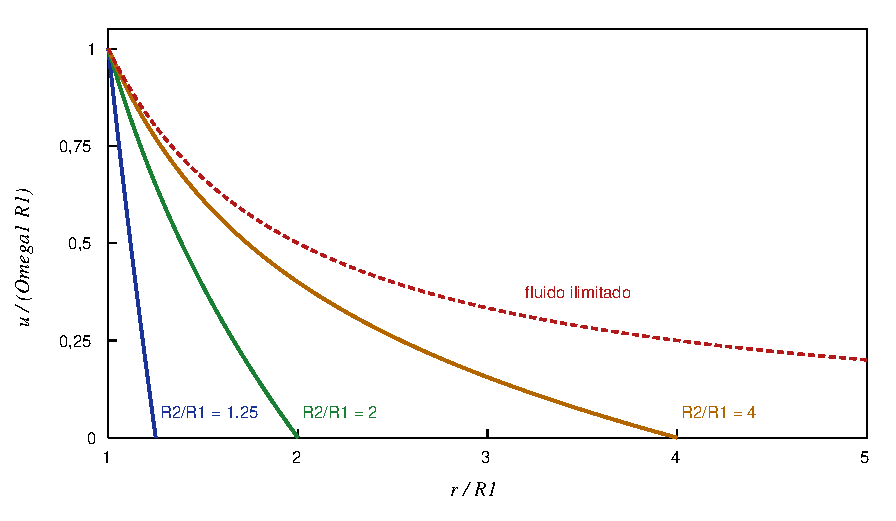
\includegraphics{../figures/FIG-0051/figure.pdf}}%
\count0=\ht0
\advance\count0 by \dp0
\count2=\wd0
\count4=\dimexpr\textheight/100*38\relax
\count6=\linewidth
\ifnum\count0<1
\count0=1
\fi
\ifnum\count2<1
\count2=1
\fi
\divide\count0 by 4096
\divide\count2 by 4096
\divide\count4 by 4096
\divide\count6 by 4096
\ifnum\count0<1
\count0=1
\fi
\ifnum\count2<1
\count2=1
\fi
\ifnum\count4<1
\count4=1
\fi
\ifnum\count6<1
\count6=1
\fi
\count8=\count2
\ifnum\count0>\count4
\count8=\numexpr\count2*\count4/\count0\relax
\fi
\ifnum\count8>\count6
\resizebox{\linewidth}{!}{\box0}%
\else
\ifnum\count0>\count4
\resizebox{!}{\dimexpr\textheight/100*38\relax}{\box0}%
\else
\box0%
\fi
\fi
\endgroup
\par\nopagebreak
\studiumcaption{fig:c06-circular}{Perfil adimensional de velocidad \(u_\theta/(\Omega_1 R_1)\) del flujo de Couette circular con el cilindro exterior fijo, para \(R_2/R_1 = 1.25\), 2 y 4, y del cilindro aislado en un fluido ilimitado (\(R_2 \to \infty\), \(u_\theta = \Omega_1 R_1^{2}/r\), trazo discontinuo). Calculado con la ecuación del perfil \(A r + B/r\).}
\end{minipage}
\par\vspace{\baselineskip}

\section{Flujo de Poiseuille entre placas}

Si además se impone un gradiente de presión uniforme en la dirección del flujo, que conviene escribir como \(G = -dp/dx\), positivo cuando la presión disminuye aguas abajo, la ecuación \(\eqref{eq:c06-balance}\) con la ley de Newton queda \(\mu\,d^{2}u/dy^{2} = -G\). Integrando dos veces e imponiendo las mismas condiciones de contorno se obtiene
\begin{equation}
u(y) = \frac{G}{2\mu}\,y\,(h - y) + U\,\frac{y}{h}, \label{eq:c06-couette}
\end{equation}
superposición de un perfil lineal debido al arrastre de la placa y de un perfil parabólico debido al gradiente de presión; la superposición es legítima porque la ecuación es lineal. El parámetro adimensional \(P = G h^{2}/(2\mu U)\) mide la importancia relativa de ambos mecanismos, y la figura~\ref{fig:c06-perfiles} muestra los perfiles para varios valores. Con un gradiente favorable (\(P\,>\,0\)) el perfil se abomba hacia delante; con uno adverso (\(P\,<\,0\)) se frena y, para \(P\,<\,-1\), el esfuerzo en la placa fija cambia de signo y aparece una zona de flujo inverso junto a ella. Este comportamiento anticipa un fenómeno central de la aerodinámica: un gradiente de presión adverso puede invertir el flujo junto a una pared y provocar el desprendimiento de la capa límite.

Cuando ambas placas están fijas, \(U = 0\), el flujo es el de Poiseuille plano: un perfil parabólico simétrico respecto al plano medio, con velocidad máxima \(u_{\max} = G h^{2}/(8\mu)\) en el centro. Integrando el perfil se obtiene el caudal por unidad de anchura,
\begin{equation}
q = \int_0^{h} u\,dy = \frac{G h^{3}}{12\mu}, \label{eq:c06-caudal-plano}
\end{equation}
y la velocidad media \(\bar u = q/h = \tfrac{2}{3}u_{\max}\). El esfuerzo en las paredes vale \(\tau_w = G h/2\), que coincide con el valor que da un equilibrio de fuerzas global sobre toda la capa de fluido. La dependencia del caudal con el cubo de la holgura tiene consecuencias prácticas notables: en una servoválvula hidráulica, reducir a la mitad la holgura entre la corredera y su camisa divide por ocho la fuga, y una holgura de unas pocas micras basta para mantener presiones de decenas de megapascales con fugas pequeñas. El mismo modelo, con \(h\) variable lentamente a lo largo de \(x\), es el punto de partida de la teoría de la lubricación hidrodinámica que explica cómo un cojinete sustenta cargas de miles de newtons sobre una película de aceite.

\section{Flujo de Hagen-Poiseuille en tubos}

El flujo en un tubo circular de radio \(R\) se trata de la misma manera en coordenadas cilíndricas. En flujo completamente desarrollado la velocidad solo depende de la distancia \(r\) al eje, \(u = u(r)\). Aislemos un cilindro de fluido coaxial de radio \(r\) y longitud \(L\). Sobre sus bases actúa una fuerza neta de presión \(G L\,\pi r^{2}\) hacia aguas abajo, donde \(G = \Delta p/L\), y sobre su superficie lateral un esfuerzo cortante \(\tau\) que se opone al movimiento. El equilibrio da
\begin{equation}
\tau(r) = \frac{G r}{2}, \qquad \tau_w = \frac{G R}{2} = \frac{\Delta p\,R}{2L}. \label{eq:c06-tau}
\end{equation}
Este resultado procede solo de un equilibrio de fuerzas y no depende de la ley constitutiva, de modo que es válido también para el esfuerzo medio en un flujo turbulento completamente desarrollado. Si el flujo es laminar y el fluido newtoniano, \(\tau = -\mu\,du/dr\), y la integración con la condición de no deslizamiento \(u(R) = 0\) conduce al perfil parabólico de Hagen-Poiseuille,
\begin{equation}
u(r) = \frac{G}{4\mu}\left(R^{2} - r^{2}\right), \label{eq:c06-perfil-tubo}
\end{equation}
representado en la figura~\ref{fig:c06-tubo}. La ley fue establecida experimentalmente por Hagen y por Poiseuille hacia 1840, este último interesado en la circulación de la sangre en los capilares, y justificada teóricamente por Stokes en 1845.

Integrando el perfil sobre la sección se obtiene el caudal, \(Q = \int_0^{R} u\,2\pi r\,dr = \pi G R^{4}/(8\mu)\), que despejando la caída de presión da la ley de Hagen-Poiseuille,
\begin{equation}
\Delta p = \frac{8\mu L Q}{\pi R^{4}}. \label{eq:c06-hagen}
\end{equation}
La velocidad media es \(V = Q/(\pi R^{2}) = G R^{2}/(8\mu)\), la mitad de la velocidad en el eje, y el esfuerzo en la pared puede escribirse como \(\tau_w = 8\mu V/D\). La dependencia con la cuarta potencia del radio es aún más acusada que en el caso plano: a igual caída de presión, duplicar el diámetro multiplica el caudal por dieciséis. En ingeniería se acostumbra a expresar la pérdida de presión mediante el factor de fricción de Darcy, \(f_D = 8\tau_w/(\rho V^{2})\), de modo que \(\Delta p = f_D\,(L/D)\,\tfrac12\rho V^{2}\); para el flujo de Hagen-Poiseuille resulta
\begin{equation}
f_D = \frac{64}{\mathrm{Re}}, \qquad \mathrm{Re} = \frac{\rho V D}{\mu}, \label{eq:c06-factor}
\end{equation}
donde \(\mathrm{Re}\) es el número de Reynolds basado en el diámetro. Para el flujo del problema resuelto de este capítulo, con \(\mathrm{Re} \approx 1352.8\), resulta un factor de fricción \(f_D \approx 0.04731\). En régimen laminar el factor de fricción no depende de la rugosidad de la pared, y la pérdida de presión es proporcional a la velocidad media; en régimen turbulento crecerá aproximadamente con su cuadrado. El capítulo 10 retoma el factor de fricción desde el punto de vista del análisis dimensional.

\section{Flujos en canales y tubos reales}

Las soluciones anteriores son exactas, pero solo describen la realidad si el flujo es laminar. Osborne Reynolds mostró en 1883 que el régimen depende de un único grupo adimensional, el número de Reynolds. En tubos de laboratorio con entradas cuidadas se observa flujo laminar completamente desarrollado por debajo de \(\mathrm{Re}_D \approx 2300\) y turbulento por encima de unos 2900, con una zona de transición intermitente entre ambos; distintas fuentes sitúan el valor crítico entre 1800 y 2300 según las perturbaciones de la instalación. Hay que subrayar que este valor no es una constante física, sino el resultado de que el flujo de Hagen-Poiseuille, que es linealmente estable, se vuelva sensible a perturbaciones finitas presentes en cualquier instalación real. En régimen turbulento el perfil medio de velocidad es mucho más plano en el centro y mucho más pronunciado junto a la pared, el esfuerzo en la pared es mayor que el laminar con el mismo caudal y la caída de presión es mayor que la prevista por la ecuación \(\eqref{eq:c06-hagen}\).

Ningún conducto real es infinitamente largo. Cerca de la entrada, el fluido llega con un perfil aproximadamente uniforme y la condición de no deslizamiento frena primero las capas próximas a la pared; esa influencia se propaga hacia el eje como una capa límite que crece hasta llenar la sección. Por conservación de la masa, el núcleo central se acelera mientras tanto. A partir de cierta distancia, la longitud de entrada, el perfil deja de cambiar y el flujo está completamente desarrollado. En régimen laminar la longitud de entrada hidrodinámica es aproximadamente \(L_h \approx 0.0575\,\mathrm{Re}_D\,D\); para \(\mathrm{Re}_D = 1500\) son \(0.0575\cdot 1500 = 86.25\) diámetros, una longitud nada despreciable. En la región de entrada el esfuerzo en la pared y la caída de presión son mayores que en el flujo desarrollado, de modo que aplicar la ley de Hagen-Poiseuille a un tubo corto subestima la pérdida de presión. En régimen turbulento la longitud de entrada es mucho menor, del orden de una a varias decenas de diámetros. Para conductos de sección no circular se usa el diámetro hidráulico \(D_h = 4A/P\), cociente entre cuatro veces el área y el perímetro mojado, que para un tubo circular coincide con el diámetro y para dos placas muy anchas separadas una distancia \(h\) vale \(2\,h\). Es una aproximación razonable en régimen turbulento, pero no exacta en laminar, donde cada geometría tiene su propio coeficiente en lugar de 64.

Las mismas ideas que dieron el flujo de Couette plano se aplican a una geometría muy frecuente en ingeniería: un eje que gira dentro de una carcasa, o un cilindro que gira dentro de un fluido. Consideremos dos cilindros coaxiales indefinidos de radios \(R_1 < R_2\) que giran alrededor de su eje común con velocidades angulares \(\Omega_1\) y \(\Omega_2\), con un fluido newtoniano en el espacio anular. Lo natural es usar coordenadas cilíndricas \((r, \theta, z)\) con el eje \(z\) a lo largo de los cilindros, porque las superficies sólidas son superficies \(r = \) constante. Buscamos un flujo estacionario y laminar en el que cada partícula describe una circunferencia alrededor del eje: la velocidad solo tiene componente azimutal, \(\mathbf{u} = u_\theta(r)\,\mathbf{e}_\theta\), y depende solo de la distancia al eje. Es el flujo de Couette circular, también llamado de Taylor-Couette. Las condiciones de contorno son las de no deslizamiento: el fluido en contacto con cada cilindro gira con él, \(u_\theta(R_1) = \Omega_1 R_1\) y \(u_\theta(R_2) = \Omega_2 R_2\).

El paso delicado es el esfuerzo cortante. En coordenadas cilíndricas el esfuerzo sobre una superficie \(r = \) constante en la dirección \(\theta\) no es \(\mu\,du_\theta/dr\), sino
\begin{equation}
\tau_{r\theta} = \mu\, r\,\frac{d}{dr}\!\left(\frac{u_\theta}{r}\right), \label{eq:c06-tau-rtheta}
\end{equation}
es decir, la viscosidad multiplicada por la variación radial de la velocidad angular \(u_\theta/r\). La razón física es clara: un fluido que gira como un sólido rígido, \(u_\theta = \Omega r\), no se deforma y no puede soportar esfuerzos viscosos, aunque la derivada \(du_\theta/dr\), que vale \(\Omega\), no sea nula. Aislemos ahora la capa de fluido comprendida entre los radios \(r\) y \(r + dr\), por unidad de longitud axial. La superficie interior, de área \(2\pi r\), soporta el esfuerzo \(\tau_{r\theta}\) con un brazo \(r\), de modo que el par transmitido a través del radio \(r\) es \(T'(r) = 2\pi r^{2}\,\tau_{r\theta}(r)\). Como la capa gira con velocidad constante, su momento angular no cambia y el par neto sobre ella es nulo: el par que recibe por dentro es el que entrega por fuera. Por tanto \(r^{2}\,\tau_{r\theta} = C\), una constante, y con \(\eqref{eq:c06-tau-rtheta}\) la ecuación del perfil es \(r^{3}\,d(u_\theta/r)/dr = C/\mu\). Integrando dos veces e imponiendo las condiciones de no deslizamiento se obtiene
\begin{equation}
u_\theta(r) = A\,r + \frac{B}{r},\qquad A = \frac{\Omega_2 R_2^{2} - \Omega_1 R_1^{2}}{R_2^{2} - R_1^{2}},\qquad B = \frac{(\Omega_1 - \Omega_2)\,R_1^{2} R_2^{2}}{R_2^{2} - R_1^{2}}. \label{eq:c06-couette-circular}
\end{equation}
El primer término es una rotación de sólido rígido, que no produce esfuerzos; el segundo es un torbellino libre, irrotacional, y es el único que transmite par. La figura~\ref{fig:c06-circular} muestra el perfil cuando el cilindro exterior está fijo.

Sustituyendo el perfil en \(\eqref{eq:c06-tau-rtheta}\), el término \(A r\) desaparece y queda \(\tau_{r\theta} = -2\mu B/r^{2}\). El signo negativo indica que, si el cilindro interior gira más deprisa que el exterior (\(B\,>\,0\)), el fluido situado fuera de cada superficie frena al situado dentro. El par que el motor debe aplicar al cilindro interior, por unidad de longitud, es igual y opuesto al que le aplica el fluido:
\begin{equation}
T' = \frac{4\pi\mu\,(\Omega_1 - \Omega_2)\,R_1^{2} R_2^{2}}{R_2^{2} - R_1^{2}}. \label{eq:c06-par-circular}
\end{equation}
El mismo par, con signo contrario, actúa sobre el cilindro exterior, lo que permite medir la viscosidad con un viscosímetro de cilindros coaxiales: se hace girar uno y se mide el par necesario para mantener el otro inmóvil. Conviene comprobar el resultado en el límite de holgura pequeña, con \(R_2\) igual a \(R_1 + h\) y \(h \ll R_1\): entonces \(R_2^{2} - R_1^{2} \approx 2R_1 h\) y el par se reduce a \(2\pi\mu\,(\Omega_1 - \Omega_2)\,R_1^{3}/h\), que es exactamente el esfuerzo del flujo de Couette plano, \(\mu\,(\Omega_1 - \Omega_2)R_1/h\), multiplicado por el área \(2\pi R_1\) y por el brazo \(R_1\). La geometría curva solo importa cuando la holgura no es pequeña frente al radio.

Un caso distinto, que no debe confundirse con el anterior, es el de un único cilindro de radio \(R\) que gira con velocidad angular \(\Omega\) dentro de un fluido ilimitado que permanece en reposo lejos de él. Formalmente es el límite de \(\eqref{eq:c06-couette-circular}\) con el cilindro exterior en reposo y \(R_2 \to \infty\): entonces \(A \to 0\) y \(B \to \Omega R^{2}\), de modo que el fluido se mueve como un torbellino libre,
\begin{equation}
u_\theta = \frac{\Omega R^{2}}{r},\qquad T' = 4\pi\mu\Omega R^{2},\qquad \dot W' = T'\,\Omega = 4\pi\mu\Omega^{2}R^{2}, \label{eq:c06-cilindro-aislado}
\end{equation}
donde \(\dot W'\) es la potencia que suministra el motor por unidad de longitud de cilindro. Tres diferencias con el flujo entre cilindros merecen subrayarse. Primero, la velocidad decae como \(\tfrac{1}{r}\) en lugar de anularse en una pared exterior, y el flujo es irrotacional en todo el fluido aunque sea viscoso. Segundo, el par es menor que con una carcasa: para un eje de 25 mm de radio dentro de una carcasa de 30 mm, el factor \(R_2^{2}/(R_2^{2} - R_1^{2})\) vale \(0.030^2/(0.030^2 - 0.025^2) = 3.273\), de modo que la carcasa multiplica por más de tres el par y la potencia. Tercero, la potencia depende del cuadrado de la velocidad angular: al ser la potencia el producto del par por \(\Omega\), olvidar ese factor da un resultado con las dimensiones de un par, no de una potencia. Toda esa potencia se disipa en calor dentro del fluido, como se comprobará en el capítulo 14 integrando la función de disipación.

\begin{tcolorbox}[title={Consejo}, studiumtip, breakable]

Antes de usar la ley de Hagen-Poiseuille, compruebe dos condiciones: que el número de Reynolds basado en el diámetro sea menor que unos 2000 y que el tramo sea varias veces más largo que la longitud de entrada, \(0.0575\,\mathrm{Re}_D\,D\). Si alguna falla, el resultado solo es una cota inferior de la caída de presión.

En los problemas de cilindros giratorios, compruebe siempre cuatro cosas: que usa el esfuerzo \(\mu\,r\,d(u_\theta/r)/dr\) y no \(\mu\,du_\theta/dr\); que el par lleva el área \(2\pi R\) por unidad de longitud y además el brazo \(R\); que la potencia es el par por la velocidad angular; y qué condición de contorno exterior corresponde al enunciado, pared a distancia finita o fluido en reposo en el infinito. Si el cilindro interior gira muy deprisa, el flujo laminar se vuelve inestable y aparecen los torbellinos de Taylor; las fórmulas solo valen por debajo de ese umbral.
\end{tcolorbox}

\begin{tcolorbox}[title={Definición}, studiumdef, breakable]

Factor de fricción de Darcy: \(f_D = 8\tau_w/(\rho V^{2})\), cociente adimensional entre el esfuerzo medio en la pared y la presión dinámica basada en la velocidad media; con él, la pérdida de presión en un tramo recto es \(\Delta p = f_D\,(L/D)\,\tfrac12\rho V^{2}\). En régimen laminar depende solo del número de Reynolds; en régimen turbulento depende también de la rugosidad relativa de la pared.
\end{tcolorbox}



% Revision bibliografica 2026: material original, contrastes verificables.

\section{Contraste bibliográfico: recirculación local en Couette--Poiseuille}
\label{sec:ref26-couette}

En un canal de separación \(h\), pared inferior fija y superior que se mueve a velocidad \(U>0\), sea \(G=-dp/dx\) el \emph{gradiente de presión impulsor}. Para fluido newtoniano de viscosidad constante, régimen estacionario, bidimensional, completamente desarrollado y sin deslizamiento, el balance de momento \(0=-dp/dx+\mu\,d^2u/dy^2\) da
\begin{equation}
u(y)=U\frac yh+\frac{G}{2\mu}\,y(h-y),\quad
q=\int_0^h u(y)\,dy=\frac{Uh}{2}+\frac{Gh^3}{12\mu}.
\label{eq:ref26-couette-q}
\end{equation}
La velocidad puede cambiar de signo cerca de la pared inferior aunque el \emph{caudal neto} conserve el signo positivo. Definiendo \(P=Gh^2/(2\mu U)\), la pendiente en \(y=0\) es \(du/dy|_0=(U/h)(1+P)\). La inversión local exige \(P<-1\), mientras que el caudal neto es positivo siempre que \(P>-3\). Así, \(-3<P<-1\) describe exactamente un flujo neto hacia delante con contraflujo junto a la pared fija. Este resultado es algebraico y no demuestra, por sí solo, que el flujo real sea estable ante perturbaciones tridimensionales.

\begin{tcolorbox}[title={Ejemplo guiado original: caudal y esfuerzos}, studiumdef, breakable]
Con \(h=0{,}002\,\mathrm{m}\), \(U=0{,}4\,\mathrm{m\,s^{-1}}\), \(\mu=0{,}020\,\mathrm{Pa\,s}\) y \(G=-8000\,\mathrm{Pa\,m^{-1}}\), resulta \(P=-2\) y \(dp/dx=+8000\,\mathrm{Pa\,m^{-1}}\), un gradiente adverso. La distribución es
\[
 u(y)=200\,y(1000y-1)\quad\text{(en SI, con \(y\) en metros)}.
\]
En \(0<y<0{,}001\,\mathrm{m}\) el fluido retrocede; en la otra mitad avanza. Sin embargo,
\[
 q=\frac{0{,}4\cdot0{,}002}{2}
    -\frac{8000(0{,}002)^3}{12\cdot0{,}020}
   =\mathbf{1{,}3333\cdot10^{-4}\,\mathrm{m^2\,s^{-1}}}>0.
\]
Los esfuerzos \emph{internos} \(\tau_{xy}=\mu\,du/dy\) en ambas paredes son \(\tau_{xy}(0)=-4\,\mathrm{Pa}\) y \(\tau_{xy}(h)=+12\,\mathrm{Pa}\). Al calcular fuerzas \emph{sobre las paredes}, debe utilizarse la normal y el signo correspondientes: no son automáticamente esos mismos vectores de tracción. La comprobación dimensional de \(q\) arroja \(\mathrm{m^2\,s^{-1}}\), al tratarse de caudal por unidad de anchura.
\end{tcolorbox}

\textbf{Autocomprobación.} Obtenga los valores de \(P\) que producen (i) pendiente nula en la pared fija, (ii) caudal neto nulo y (iii) ausencia de gradiente de presión. Justifique cuándo la condición de no deslizamiento y el supuesto de flujo desarrollado podrían fallar. Deducción y datos numéricos originales, contrastados conceptualmente con White, secciones 4.10 y 6,4 \cite{ref26-white}, y Shaughnessy, Katz y Schaffer \cite{ref26-shaughnessy}.


\section{Desarrollos y práctica}

Las deducciones de este capítulo son soluciones exactas de las ecuaciones de Navier-Stokes obtenidas aquí por equilibrio de fuerzas sobre un elemento de fluido \(\eqref{eq:c06-balance}\): el flujo de Couette con gradiente de presión \(\eqref{eq:c06-couette}\), su caudal \(\eqref{eq:c06-caudal-plano}\), el esfuerzo en la pared de un tubo \(\eqref{eq:c06-tau}\), la ley de Hagen-Poiseuille \(\eqref{eq:c06-hagen}\) y el factor de fricción laminar \(\eqref{eq:c06-factor}\). En el capítulo 14 se recuperarán como casos particulares de las ecuaciones generales. Antes de aplicar cualquiera de ellas en un ejercicio hay que comprobar que el flujo es laminar y que el tramo considerado está más allá de la longitud de entrada.

\begin{tcolorbox}[title={Desarrollos del modelo}, studiumdef, breakable]

\noindent\textbf{Flujo de Couette con gradiente de presión}

\[
u(y) = \frac{G}{2\mu}\,y\,(h - y) + U\,\frac{y}{h},\qquad G = -\frac{dp}{dx}
\]

\noindent\textbf{Hipótesis}
\begin{itemize}
\item flujo estacionario, incompresible, laminar y completamente desarrollado
\item placas planas, paralelas e infinitas
\item gradiente de presión uniforme
\end{itemize}

\noindent\textbf{Limitaciones}
\begin{itemize}
\item laminar: deja de valer al aparecer la turbulencia
\end{itemize}

\noindent\textbf{Pasos}
\begin{enumerate}
\item
balance de fuerzas en una lámina de fluido: d tau/dy = dp/dx

\[
\frac{d\tau}{dy} = \frac{dp}{dx} = -G
\]
\item
ley de Newton de la viscosidad

\[
\mu\,\frac{d^{2}u}{dy^{2}} = -G
\]
\item
integrar dos veces con u(0) = 0 y u(h) = U

\[
u(y) = \frac{G}{2\mu}\,y\,(h - y) + U\,\frac{y}{h}
\]
\item
relación usada en el texto (paso intermedio no comprobado por separado)

\[
G = 0:\quad u = Uy/h,\qquad q = Uh/2
\]
\end{enumerate}

\noindent\textbf{Variables}
\begin{itemize}
\item $U$: velocidad de la placa superior ($\mathrm{m}\,\mathrm{s}^{-1}$)
\item $h$: separación entre placas ($\mathrm{m}$)
\end{itemize}



\noindent\textbf{Caudal del flujo de Poiseuille plano}

\begin{equation}
q = \int_0^{h} u\,dy = \frac{G h^{3}}{12\mu},\qquad u_{\max} = \frac{G h^{2}}{8\mu},\qquad \bar u = \tfrac{2}{3}u_{\max}
\label{eq:c06-poiseuille-plano}
\end{equation}

\noindent\textbf{Hipótesis}
\begin{itemize}
\item placas fijas (U = 0)
\item mismas hipótesis que el flujo de Couette
\end{itemize}

\noindent\textbf{Limitaciones}
\begin{itemize}
\item la dependencia con h al cubo hace la fuga muy sensible a la holgura
\end{itemize}

\noindent\textbf{Pasos}
\begin{enumerate}
\item
integrar el perfil parabólico entre las placas

\[
q = \frac{G}{2\mu}\int_0^{h} y\,(h - y)\,dy = \frac{G h^{3}}{12\mu}
\]
\item
evaluar el perfil en el plano medio

\[
u_{\max} = u\!\left(\tfrac{h}{2}\right) = \frac{G h^{2}}{8\mu}
\]
\item
dividir el caudal por h

\[
\bar u = \frac{q}{h} = \tfrac{2}{3}\,u_{\max}
\]
\item
relación usada en el texto (paso intermedio no comprobado por separado)

\[
\bar u = q/h = \tfrac{2}{3}u_{\max}
\]
\end{enumerate}

\noindent\textbf{Variables}
\begin{itemize}
\item $q$: caudal por unidad de anchura ($\mathrm{m}^{2}\,\mathrm{s}^{-1}$)
\end{itemize}



\noindent\textbf{Esfuerzo en la pared de un tubo por equilibrio de fuerzas}

\begin{equation}
\tau(r) = \frac{G r}{2},\qquad \tau_w = \frac{G R}{2} = \frac{\Delta p\,R}{2L}
\label{eq:c06-tau-pared}
\end{equation}

\noindent\textbf{Hipótesis}
\begin{itemize}
\item flujo estacionario y completamente desarrollado en un tubo recto
\item válido tanto en régimen laminar como para el esfuerzo medio en turbulento
\end{itemize}

\noindent\textbf{Limitaciones}
\begin{itemize}
\item no se usa ninguna ley constitutiva: el resultado no depende de la viscosidad
\end{itemize}

\noindent\textbf{Pasos}
\begin{enumerate}
\item
equilibrio de un cilindro de fluido coaxial de radio r y longitud L

\[
G L\,\pi r^{2} = \tau\,2\pi r L
\]
\item
la fuerza de presión neta se equilibra con el esfuerzo cortante en su superficie lateral

\[
\tau = \frac{G r}{2}
\]
\end{enumerate}

\noindent\textbf{Variables}
\begin{itemize}
\item $R$: radio del tubo ($\mathrm{m}$)
\end{itemize}



\noindent\textbf{Ley de Hagen-Poiseuille}

\[
u(r) = \frac{G}{4\mu}\left(R^{2} - r^{2}\right),\qquad Q = \frac{\pi G R^{4}}{8\mu},\qquad \Delta p = \frac{8\mu L Q}{\pi R^{4}}
\]

\noindent\textbf{Hipótesis}
\begin{itemize}
\item fluido newtoniano e incompresible
\item flujo laminar, estacionario y completamente desarrollado
\item tubo circular recto de radio constante
\end{itemize}

\noindent\textbf{Limitaciones}
\begin{itemize}
\item falla si el flujo es turbulento o si el tramo es comparable a la longitud de entrada
\end{itemize}

\noindent\textbf{Pasos}
\begin{enumerate}
\item
igualar tau = -mu du/dr con G r/2

\[
-\mu\,\frac{du}{dr} = \frac{G r}{2}
\]
\item
integrar con u(R) = 0

\[
u(r) = \frac{G}{4\mu}\left(R^{2} - r^{2}\right)
\]
\item
integrar el perfil sobre la sección para obtener el caudal

\[
Q = \int_0^{R} u\,2\pi r\,dr = \frac{\pi G R^{4}}{8\mu}
\]
\item
relación usada en el texto (paso intermedio no comprobado por separado)

\[
\tau = -\mu\,du/dr
\]
\item
relación usada en el texto (paso intermedio no comprobado por separado)

\[
V = Q/(\pi R^{2}) = G R^{2}/(8\mu)
\]
\end{enumerate}

\noindent\textbf{Variables}
\begin{itemize}
\item $Q$: caudal ($\mathrm{m}^{3}\,\mathrm{s}^{-1}$)
\item $L$: longitud del tramo ($\mathrm{m}$)
\end{itemize}



\noindent\textbf{Factor de fricción laminar}

\begin{equation}
f_D \equiv \frac{8\tau_w}{\rho V^{2}} = \frac{64}{\mathrm{Re}},\qquad \mathrm{Re} = \frac{\rho V D}{\mu}
\label{eq:c06-factor-laminar}
\end{equation}

\noindent\textbf{Hipótesis}
\begin{itemize}
\item flujo de Hagen-Poiseuille
\end{itemize}

\noindent\textbf{Limitaciones}
\begin{itemize}
\item solo para régimen laminar, aproximadamente Re < 2300
\end{itemize}

\noindent\textbf{Pasos}
\begin{enumerate}
\item
expresar el esfuerzo en la pared con la velocidad media: tau\(_w = 8\) mu V/D

\[
\tau_w = \frac{G R}{2} = \frac{8\mu V}{D}
\]
\item
sustituir en la definición del factor de fricción

\[
f_D = \frac{64\,\mu}{\rho V D} = \frac{64}{\mathrm{Re}}
\]
\end{enumerate}

\noindent\textbf{Variables}
\begin{itemize}
\item $V$: velocidad media ($\mathrm{m}\,\mathrm{s}^{-1}$)
\end{itemize}



\noindent\textbf{Perfil de velocidad del flujo de Couette circular por equilibrio de pares}

\[
u_\theta(r) = A\,r + \frac{B}{r},\qquad A = \frac{\Omega_2 R_2^{2} - \Omega_1 R_1^{2}}{R_2^{2} - R_1^{2}},\qquad B = \frac{(\Omega_1 - \Omega_2)\,R_1^{2} R_2^{2}}{R_2^{2} - R_1^{2}}
\]

\noindent\textbf{Hipótesis}
\begin{itemize}
\item flujo estacionario, laminar e incompresible
\item cilindros coaxiales infinitamente largos, sin efectos de extremo
\item velocidad solo azimutal y función solo de r
\item sin gravedad ni gradiente de presión azimutal
\end{itemize}

\noindent\textbf{Principios}
\begin{itemize}
\item equilibrio de momentos sobre una capa cilíndrica de fluido
\item ley de Newton de la viscosidad en coordenadas cilíndricas
\end{itemize}

\noindent\textbf{Condiciones de contorno}
\begin{itemize}
\item \(u_theta(R1) =\) Omega1 R1
\item \(u_theta(R2) =\) Omega2 R2
\end{itemize}

\noindent\textbf{Aplicabilidad}
\begin{itemize}
\item viscosímetros de cilindros coaxiales
\item cojinetes de holgura grande
\item ejes que giran dentro de una carcasa
\end{itemize}

\noindent\textbf{Limitaciones}
\begin{itemize}
\item inestable (torbellinos de Taylor) si el cilindro interior gira suficientemente deprisa
\item sin efectos de extremo ni flujo axial
\end{itemize}

\noindent\textbf{Pasos}
\begin{enumerate}
\item
par transmitido a través de la superficie de radio r por unidad de longitud

\[
T'(r) = 2\pi r^{2}\,\tau_{r\theta}(r)
\]
\item
en régimen estacionario el par no depende de r

\[
r^{2}\,\tau_{r\theta} = C
\]
\item
esfuerzo newtoniano en coordenadas cilíndricas

\[
\tau_{r\theta} = \mu\, r\,\frac{d}{dr}\!\left(\frac{u_\theta}{r}\right)
\]
\item
integrar e imponer el no deslizamiento en r = R1 y r = R2

\[
u_\theta(R_1) = \Omega_1 R_1,\qquad u_\theta(R_2) = \Omega_2 R_2
\]
\end{enumerate}

\noindent\textbf{Variables}
\begin{itemize}
\item $R_{1}$: radio del cilindro interior ($\mathrm{m}$)
\item $R_{2}$: radio del cilindro exterior ($\mathrm{m}$)
\item $A$: velocidad angular del término de rotación rígida ($\mathrm{1/s}$)
\item $B$: intensidad del término de torbellino libre ($\mathrm{m}^{2}\,\mathrm{s}^{-1}$)
\end{itemize}



\noindent\textbf{Par por unidad de longitud entre cilindros coaxiales}

\[
T' = \frac{4\pi\mu\,(\Omega_1 - \Omega_2)\,R_1^{2} R_2^{2}}{R_2^{2} - R_1^{2}}
\]

\noindent\textbf{Hipótesis}
\begin{itemize}
\item flujo de Couette circular laminar y estacionario
\end{itemize}

\noindent\textbf{Principios}
\begin{itemize}
\item par = esfuerzo por área por brazo
\end{itemize}

\noindent\textbf{Limitaciones}
\begin{itemize}
\item es el par del motor; el fluido ejerce sobre el cilindro un par igual y opuesto
\end{itemize}

\noindent\textbf{Pasos}
\begin{enumerate}
\item
esfuerzo del perfil: solo el término B/r produce esfuerzo

\[
\tau_{r\theta} = -\frac{2\mu B}{r^{2}}
\]
\item
par que hay que aplicar al cilindro interior por unidad de longitud

\[
T' = 2\pi R_1^{2}\,\frac{2\mu B}{R_1^{2}} = 4\pi\mu B
\]
\end{enumerate}

\noindent\textbf{Variables}
\begin{itemize}
\item $T'$: par por unidad de longitud ($\mathrm{N}$)
\end{itemize}



\noindent\textbf{Cilindro giratorio en un fluido ilimitado en reposo}

\[
u_\theta = \frac{\Omega R^{2}}{r},\qquad T' = 4\pi\mu\Omega R^{2},\qquad \dot W' = T'\,\Omega = 4\pi\mu\Omega^{2}R^{2}
\]

\noindent\textbf{Hipótesis}
\begin{itemize}
\item fluido en reposo lejos del cilindro (Omega2 = 0 y R2 tendiendo a infinito)
\item régimen estacionario ya alcanzado
\end{itemize}

\noindent\textbf{Principios}
\begin{itemize}
\item límite del flujo de Couette circular
\item potencia = par por velocidad angular
\end{itemize}

\noindent\textbf{Limitaciones}
\begin{itemize}
\item el régimen estacionario en un fluido ilimitado solo se alcanza asintóticamente
\item a número de Reynolds alto el flujo deja de ser laminar
\end{itemize}

\noindent\textbf{Pasos}
\begin{enumerate}
\item
límite R2 -> infinito con Omega2 = 0: A -> 0 y B -> Omega \(R^2\)

\[
A \to 0,\qquad B \to \Omega R^{2}
\]
\item
par del motor por unidad de longitud

\[
T' = 4\pi\mu\Omega R^{2}
\]
\item
potencia por unidad de longitud

\[
\dot W' = 4\pi\mu\Omega^{2}R^{2}
\]
\end{enumerate}

\noindent\textbf{Variables}
\begin{itemize}
\item $R$: radio del cilindro ($\mathrm{m}$)
\item $\dot W'$: potencia por unidad de longitud ($\mathrm{W}\,\mathrm{m}^{-1}$)
\end{itemize}


\end{tcolorbox}

\begin{tcolorbox}[title={Problema resuelto}, studiumworked, breakable]

\noindent\textbf{Enunciado}
Una línea hidráulica de una aeronave tiene un diámetro interior de 6.0 mm y 3.0 m de longitud y transporta \(1.5\times 10^{-4}\) m\(^3\)/s de un aceite hidráulico de densidad 850 kg/m\(^3\) y viscosidad \(0.020\) Pa s. (a) Compruebe que el flujo es laminar. (b) Calcule la caída de presión en el tramo, suponiendo flujo completamente desarrollado. (c) Calcule la potencia disipada. (d) Discuta la validez de la hipótesis de flujo desarrollado.

\noindent\textbf{Datos}
\begin{itemize}
\item $D = 0.006\,\mathrm{m}$ — diámetro
\item $L = 3.0\,\mathrm{m}$ — longitud
\item $Q = 0.00015\,\mathrm{m}^{3}\,\mathrm{s}^{-1}$ — caudal
\item $\rho = 850\,\mathrm{kg}\,\mathrm{m}^{-3}$ — densidad
\item $\mu = 0.02\,\mathrm{Pa}\,\mathrm{s}$ — viscosidad
\end{itemize}

\noindent\textbf{Incógnita}
caída de presión en el tramo

\noindent\textbf{Modelo físico}

\noindent\textit{Hagen-Poiseuille}

\[
\Delta p = \frac{128\,\mu L Q}{\pi D^{4}}
\]

\noindent\textbf{Hipótesis}
\begin{itemize}
\item flujo laminar, estacionario y completamente desarrollado
\item aceite newtoniano a temperatura uniforme
\item tubo recto y liso
\end{itemize}

\noindent\textbf{Desarrollo paso a paso}

\phantomsection\label{solution:mf-006}
\noindent\textbf{Elección del procedimiento.} Antes de aplicar Hagen--Poiseuille hay que calcular la velocidad media y comprobar el régimen con Reynolds. Para flujo laminar plenamente desarrollado, $\Delta p=128\mu LQ/(\pi D^4)$; la potencia hidráulica perdida es $\Delta p\,Q$.

\begin{enumerate}

\item El dato es diámetro, por lo que el área circular lleva un factor $1/4$.

\[\fitmath{A=\frac{\pi\cdot {D}^{2}}{4}}\]

\[\fitmath{A=\frac{\pi\cdot {(0.006)}^{2}}{4}\approx 2.827433\times10^{-5}\,\mathrm{m^{2}}}\]

\item De continuidad $Q=AV$, despejar la velocidad media.

\[\fitmath{V=\frac{Q}{A}}\]

\[\fitmath{V=\frac{(0.00015)}{(2.827433388\times10^{-5})}\approx 5.305165\,\mathrm{m/s}}\]

\item Comparar inercia y viscosidad con la escala diámetro.

\[\fitmath{\mathrm{Re}=\frac{\rho\cdot V\cdot D}{\mu}}\]

\[\fitmath{\mathrm{Re}=\frac{(850)\cdot (5.30516477)\cdot (0.006)}{(0.02)}\approx 1352.817\,}\]

\item Con la estimación de entrada $L_e/D\simeq0.0575\mathrm{Re}$ usada en este capítulo, comprobar si $L_e$ es pequeño frente a $L$.

\[\fitmath{\mathrm{Le}=0.0575\cdot \mathrm{Re}\cdot D}\]

\[\fitmath{\mathrm{Le}=0.0575\cdot (1352.817016)\cdot (0.006)\approx 0.4667219\,\mathrm{m}}\]

\item Despejar la pérdida de presión de la relación caudal--presión laminar.

\[\fitmath{\mathrm{dp}=\frac{128\cdot \mu\cdot L\cdot Q}{\pi\cdot {D}^{4}}}\]

\[\fitmath{\mathrm{dp}=\frac{128\cdot (0.02)\cdot (3)\cdot (0.00015)}{\pi\cdot {(0.006)}^{4}}\approx 282942.1\,\mathrm{Pa}}\]

\item Multiplicar caída de presión por caudal, no por velocidad.

\[\fitmath{P=\mathrm{dp}\cdot Q}\]

\[\fitmath{P=(282942.1211)\cdot (0.00015)\approx 42.44132\,\mathrm{W}}\]

\end{enumerate}

\noindent\textbf{Contraste y comparación.} La estimación de entrada da aproximadamente $0.467$ m frente a 3 m. La relación de tramo plenamente desarrollado omite la pérdida adicional de entrada; su uso aquí es una aproximación, no una solución exacta de todo el conducto.


\noindent\textbf{Sustitución numérica}

\[
\frac{128 \left(3.0\,\mathrm{m}\right) \left(0.00015\,\mathrm{m}^{3}\,\mathrm{s}^{-1}\right) \left(0.02\,\mathrm{Pa}\,\mathrm{s}\right)}{\pi \left(0.006\,\mathrm{m}\right)^{4}}
\]

\noindent\textbf{Resultado}

\[
\mathrm{Re} \approx 1353,\quad \Delta p \approx 2.83\times 10^{5}\ \mathrm{Pa}\ (2.8\ \mathrm{bar}),\quad \dot W \approx 42\ \mathrm{W}
\]

\noindent\textbf{Interpretación}
El flujo es laminar, pero la longitud de entrada (unos 0.47 m) es el 16 \% del tramo: la caída real será algo mayor que la calculada. Con aceite frío, más viscoso, la caída aumentaría proporcionalmente a la viscosidad.

\noindent\textbf{Comprobación de la respuesta} la aritmética del último paso reproduce la respuesta enunciada a la precisión con que está escrita. Es una reproducción aritmética; no valida el modelo físico ni sus hipótesis.

\noindent\textbf{Limitaciones}
\begin{itemize}
\item la viscosidad del aceite hidráulico varía mucho con la temperatura
\item no incluye pérdidas en codos ni accesorios
\end{itemize}

\noindent\textbf{Errores frecuentes}
\begin{itemize}
\item usar el diámetro en lugar del radio en la fórmula con \(R^4\)
\item no comprobar el régimen antes de aplicar la ley
\end{itemize}
\end{tcolorbox}

\begin{tcolorbox}[title={Ejercicios propuestos}, studiumworked, breakable]

\noindent\textbf{1 (De examen, Desarrollo)}
Por una línea de lubricación de una turbina, de 4.0 mm de diámetro y 2.0 m de longitud, circula aceite (\(\rho = 870\) kg/m\(^3\), \(\mu = 0.012\) Pa s) con velocidad media de 1.2 m/s. Compruebe el régimen, calcule la caída de presión con el factor de fricción laminar y la potencia de bombeo necesaria.

\noindent\textbf{2 (Básico, Cálculo)}
Una placa se desliza a 3.0 m/s sobre una película de aceite de 0.50 mm de espesor y viscosidad 0.10 Pa s, sin gradiente de presión. Calcule el esfuerzo cortante y el caudal arrastrado por unidad de anchura.

\noindent\textbf{3 (Intermedio, Aplicación)}
La corredera de una servoválvula deja una holgura de 20 \(\mu\)m entre dos superficies planas, con una anchura de 10 mm y una longitud de sellado de 5.0 mm. La diferencia de presión es de 10 MPa y el aceite tiene una viscosidad de \(0.030\) Pa s. Estime la fuga con el modelo de Poiseuille plano.

\noindent\textbf{4 (Intermedio, DESIGN)}
Un viscosímetro capilar tiene un tubo de 0.50 mm de radio y 0.20 m de longitud. Con una diferencia de presión de 2000 Pa se mide un caudal de \(5.0\times 10^{-8}\) m\(^3\)/s. Determine la viscosidad del líquido.

\noindent\textbf{5 (Avanzado, Desarrollo)}
En un flujo de Couette con gradiente de presión, la placa superior se mueve a 2.0 m/s, la holgura es de 1.0 mm y la viscosidad 0.050 Pa s. Determine el gradiente de presión adverso \(dp/dx\,>\,0\) para el que el esfuerzo cortante sobre la placa fija se anula, umbral a partir del cual aparece flujo inverso junto a ella.

\noindent\textbf{6 (Intermedio, Aplicación)}
Un viscosímetro de cilindros coaxiales tiene un rotor interior de 20.0 mm de radio y una copa fija de 21.0 mm de radio; la longitud mojada es de 100 mm. Cuando el rotor gira a 10.0 rad/s el par medido es \(2.00\times 10^{-3}\) N m. Despreciando los efectos de extremo, determine la viscosidad del líquido y discuta si habría bastado la aproximación de holgura pequeña.

\noindent\textbf{7 (De examen, Desarrollo)}
En un ensayo, el cilindro interior (radio 40 mm) se mantiene fijo y el exterior (radio 50 mm) gira a 20 rad/s; entre ambos hay glicerina (\(\mu = 1.41\) Pa s) y la longitud es de 0.20 m. (a) Partiendo del equilibrio de pares sobre una capa cilíndrica, obtenga el perfil \(u_\theta(r)\). (b) Calcule el par necesario para impedir que gire el cilindro interior. (c) Calcule la potencia que suministra el motor del cilindro exterior y explique dónde se disipa.

\noindent\textbf{8 (Avanzado, COMPARATIVE)}
Un eje de 25 mm de radio gira a 150 rad/s sumergido en un gran depósito de aceite (\(\mu = 0.080\) Pa s) que puede considerarse ilimitado y en reposo lejos del eje. (a) Calcule el par y la potencia por unidad de longitud en régimen laminar estacionario. (b) Repita el cálculo si el eje gira dentro de una carcasa fija de 30 mm de radio. (c) Explique por qué los dos resultados son distintos aunque el eje y el aceite sean los mismos.
\end{tcolorbox}

\begin{tcolorbox}[title={Autoevaluación}, studiumcheck, breakable]

(1) ¿Por qué el término de aceleración desaparece en un flujo completamente desarrollado? (2) ¿Qué condición sobre \(P = Gh^{2}/(2\mu U)\) produce flujo inverso junto a la placa fija? (3) Demuestre que el esfuerzo en la pared de un tubo, \(\Delta p\,R/(2L)\), no depende de la viscosidad y explique por qué sigue siendo válido en régimen turbulento. (4) ¿En qué factor cambia el caudal de un tubo laminar si se reduce el diámetro un 10 \% manteniendo la caída de presión? (5) ¿Por qué no depende de la rugosidad el factor de fricción laminar? (6) ¿Qué error se comete al aplicar la ley de Hagen-Poiseuille a un tubo de longitud comparable a la de entrada?

(1) ¿Por qué un fluido en rotación de sólido rígido no ejerce esfuerzos viscosos aunque su velocidad crezca con el radio? (2) Demuestre, con un equilibrio de pares, que \(r^{2}\tau_{r\theta}\) es constante en el flujo de Couette circular. (3) ¿Qué término del perfil \(A r + B/r\) transmite el par? (4) ¿Cuánto vale el par si ambos cilindros giran con la misma velocidad angular? (5) Obtenga el límite de holgura pequeña del par y relaciónelo con el flujo de Couette plano. (6) ¿Por qué la potencia disipada por un cilindro en un fluido ilimitado es proporcional a \(\Omega^{2}\)?
\end{tcolorbox}
\studiumchaptercheck

\chapter{Flujos externos: resistencia y sustentación}
\label{chap:c07}

\studiumchapterguide{Un cuerpo que se mueve en el seno de un fluido, o un fluido que fluye alrededor de un cuerpo, da lugar a una fuerza que en aeronáutica se descompone en resistencia, paralela a la corriente incidente, y sustentación, perpendicular a ella. Estas dos fuerzas deciden la viabilidad de cualquier vehículo aéreo. La guía docente las incluye como caso de estudio de los flujos externos. Este capítulo explica su origen físico en las distribuciones de presión y de esfuerzo cortante, introduce los coeficientes adimensionales con que se miden y comparan, describe los distintos regímenes de la resistencia de cuerpos romos y fuselados, presenta las ideas básicas de la sustentación de un perfil y de un ala, y las aplica al vuelo horizontal y a la velocidad terminal.}

\section{Fuerzas aerodinámicas sobre cuerpos}

La fuerza que un fluido ejerce sobre un cuerpo tiene solo dos orígenes, la presión y el esfuerzo cortante, que actúan sobre cada elemento de su superficie. Si \(\mathbf{n}\) es la normal exterior al cuerpo y \(\boldsymbol{\tau}_w\) el vector esfuerzo cortante en la pared, la fuerza total es
\begin{equation}
\mathbf{F} = \oint_S \left(-p\,\mathbf{n} + \boldsymbol{\tau}_w\right) dS. \label{eq:c07-fuerza}
\end{equation}
Su componente en la dirección de la corriente incidente es la resistencia \(D\) y la perpendicular, la sustentación \(L\); en un cuerpo tridimensional aparece además una fuerza lateral. La descomposición según el origen de las tensiones da otra clasificación útil: la integral de la presión produce la resistencia de forma o de presión, que depende sobre todo de la forma y del área frontal del cuerpo, y la integral del esfuerzo cortante produce la resistencia de fricción, proporcional al área mojada. La resistencia de fricción requiere esfuerzos viscosos. En cuerpos romos, gran parte de la resistencia de presión se relaciona con la separación de la capa límite y la estela, fenómenos influidos por la viscosidad; sin embargo, no toda resistencia de presión tiene necesariamente ese origen. Un ala finita presenta resistencia inducida asociada a la sustentación, y en flujo compresible puede aparecer resistencia de onda por choques, incluso en modelos con viscosidad despreciable. Un cuerpo es romo cuando domina la resistencia de presión, como un cilindro, una esfera o un automóvil, y fuselado cuando domina la de fricción, como un perfil alar a ángulo de ataque pequeño. La figura~\ref{fig:c07-fuerzas} muestra la descomposición sobre un perfil.

\par\vspace{\baselineskip}
\noindent\begin{minipage}{\linewidth}
\centering
\begingroup
\setbox0=\hbox{\begin{tikzpicture}
\draw[thick,fill=gray!20] plot[smooth cycle] coordinates {(0,0) (0.4,0.32) (1.5,0.55) (3.0,0.42) (4.5,0.12) (5.2,0) (4.5,-0.03) (3.0,-0.08) (1.5,-0.15) (0.4,-0.17)};
\draw[->,thick] (-2.4,-0.9) -- (-0.8,-0.5) node[midway,above left]{$V_\infty$};
\draw[dashed] (0,0) -- (5.8,0); \draw[dashed] (0,0) -- (5.6,1.4);
\draw (2.2,0) arc (0:14:2.2); \node at (2.6,0.25) {\scriptsize $\alpha$};
\draw[->,very thick,blue] (1.6,0.1) -- (1.0,2.5) node[above]{$L$};
\draw[->,very thick,red] (1.6,0.1) -- (2.8,0.4) node[right]{$D$};
\draw[->,thick] (1.6,0.1) -- (1.88,1.54) node[right]{\scriptsize resultante};
\foreach \x/\y/\dx/\dy in {0.6/0.38/0.08/-0.3, 2.2/0.52/0.0/-0.3, 3.6/0.32/-0.03/-0.3} { \draw[->,teal] (\x+\dx*-1,\y+0.3) -- (\x,\y); }
\node[teal] at (2.2,1.2) {\scriptsize $-p\,\mathbf{n}$};
\draw[->,orange] (3.4,0.62) -- (4.0,0.5) node[right]{\scriptsize $\tau_w$};
\end{tikzpicture}}%
\count0=\ht0
\advance\count0 by \dp0
\count2=\wd0
\count4=\dimexpr\textheight/100*38\relax
\count6=\linewidth
\ifnum\count0<1
\count0=1
\fi
\ifnum\count2<1
\count2=1
\fi
\divide\count0 by 4096
\divide\count2 by 4096
\divide\count4 by 4096
\divide\count6 by 4096
\ifnum\count0<1
\count0=1
\fi
\ifnum\count2<1
\count2=1
\fi
\ifnum\count4<1
\count4=1
\fi
\ifnum\count6<1
\count6=1
\fi
\count8=\count2
\ifnum\count0>\count4
\count8=\numexpr\count2*\count4/\count0\relax
\fi
\ifnum\count8>\count6
\resizebox{\linewidth}{!}{\begin{tikzpicture}
\draw[thick,fill=gray!20] plot[smooth cycle] coordinates {(0,0) (0.4,0.32) (1.5,0.55) (3.0,0.42) (4.5,0.12) (5.2,0) (4.5,-0.03) (3.0,-0.08) (1.5,-0.15) (0.4,-0.17)};
\draw[->,thick] (-2.4,-0.9) -- (-0.8,-0.5) node[midway,above left]{$V_\infty$};
\draw[dashed] (0,0) -- (5.8,0); \draw[dashed] (0,0) -- (5.6,1.4);
\draw (2.2,0) arc (0:14:2.2); \node at (2.6,0.25) {\scriptsize $\alpha$};
\draw[->,very thick,blue] (1.6,0.1) -- (1.0,2.5) node[above]{$L$};
\draw[->,very thick,red] (1.6,0.1) -- (2.8,0.4) node[right]{$D$};
\draw[->,thick] (1.6,0.1) -- (1.88,1.54) node[right]{\scriptsize resultante};
\foreach \x/\y/\dx/\dy in {0.6/0.38/0.08/-0.3, 2.2/0.52/0.0/-0.3, 3.6/0.32/-0.03/-0.3} { \draw[->,teal] (\x+\dx*-1,\y+0.3) -- (\x,\y); }
\node[teal] at (2.2,1.2) {\scriptsize $-p\,\mathbf{n}$};
\draw[->,orange] (3.4,0.62) -- (4.0,0.5) node[right]{\scriptsize $\tau_w$};
\end{tikzpicture}}%
\else
\ifnum\count0>\count4
\resizebox{!}{\dimexpr\textheight/100*38\relax}{\begin{tikzpicture}
\draw[thick,fill=gray!20] plot[smooth cycle] coordinates {(0,0) (0.4,0.32) (1.5,0.55) (3.0,0.42) (4.5,0.12) (5.2,0) (4.5,-0.03) (3.0,-0.08) (1.5,-0.15) (0.4,-0.17)};
\draw[->,thick] (-2.4,-0.9) -- (-0.8,-0.5) node[midway,above left]{$V_\infty$};
\draw[dashed] (0,0) -- (5.8,0); \draw[dashed] (0,0) -- (5.6,1.4);
\draw (2.2,0) arc (0:14:2.2); \node at (2.6,0.25) {\scriptsize $\alpha$};
\draw[->,very thick,blue] (1.6,0.1) -- (1.0,2.5) node[above]{$L$};
\draw[->,very thick,red] (1.6,0.1) -- (2.8,0.4) node[right]{$D$};
\draw[->,thick] (1.6,0.1) -- (1.88,1.54) node[right]{\scriptsize resultante};
\foreach \x/\y/\dx/\dy in {0.6/0.38/0.08/-0.3, 2.2/0.52/0.0/-0.3, 3.6/0.32/-0.03/-0.3} { \draw[->,teal] (\x+\dx*-1,\y+0.3) -- (\x,\y); }
\node[teal] at (2.2,1.2) {\scriptsize $-p\,\mathbf{n}$};
\draw[->,orange] (3.4,0.62) -- (4.0,0.5) node[right]{\scriptsize $\tau_w$};
\end{tikzpicture}}%
\else
\begin{tikzpicture}
\draw[thick,fill=gray!20] plot[smooth cycle] coordinates {(0,0) (0.4,0.32) (1.5,0.55) (3.0,0.42) (4.5,0.12) (5.2,0) (4.5,-0.03) (3.0,-0.08) (1.5,-0.15) (0.4,-0.17)};
\draw[->,thick] (-2.4,-0.9) -- (-0.8,-0.5) node[midway,above left]{$V_\infty$};
\draw[dashed] (0,0) -- (5.8,0); \draw[dashed] (0,0) -- (5.6,1.4);
\draw (2.2,0) arc (0:14:2.2); \node at (2.6,0.25) {\scriptsize $\alpha$};
\draw[->,very thick,blue] (1.6,0.1) -- (1.0,2.5) node[above]{$L$};
\draw[->,very thick,red] (1.6,0.1) -- (2.8,0.4) node[right]{$D$};
\draw[->,thick] (1.6,0.1) -- (1.88,1.54) node[right]{\scriptsize resultante};
\foreach \x/\y/\dx/\dy in {0.6/0.38/0.08/-0.3, 2.2/0.52/0.0/-0.3, 3.6/0.32/-0.03/-0.3} { \draw[->,teal] (\x+\dx*-1,\y+0.3) -- (\x,\y); }
\node[teal] at (2.2,1.2) {\scriptsize $-p\,\mathbf{n}$};
\draw[->,orange] (3.4,0.62) -- (4.0,0.5) node[right]{\scriptsize $\tau_w$};
\end{tikzpicture}%
\fi
\fi
\endgroup
\par\nopagebreak
\studiumcaption{fig:c07-fuerzas}{Fuerzas sobre un perfil alar: la integral de la presión \(-p\,\mathbf{n}\) y del esfuerzo cortante \(\boldsymbol{\tau}_w\) sobre la superficie da la resultante aerodinámica, que se descompone en sustentación \(L\), perpendicular a la corriente incidente \(V_\infty\), y resistencia \(D\), paralela a ella. \(\alpha\) es el ángulo de ataque.}
\end{minipage}
\par\vspace{\baselineskip}

\par\vspace{\baselineskip}
\noindent\begin{minipage}{\linewidth}
\centering
\begingroup
\setbox0=\hbox{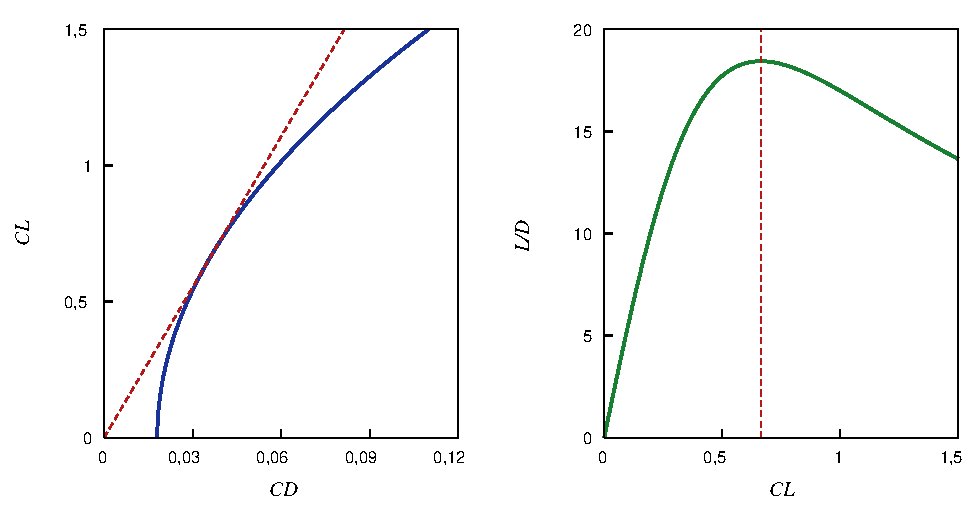
\includegraphics{../figures/FIG-0017/figure.pdf}}%
\count0=\ht0
\advance\count0 by \dp0
\count2=\wd0
\count4=\dimexpr\textheight/100*38\relax
\count6=\linewidth
\ifnum\count0<1
\count0=1
\fi
\ifnum\count2<1
\count2=1
\fi
\divide\count0 by 4096
\divide\count2 by 4096
\divide\count4 by 4096
\divide\count6 by 4096
\ifnum\count0<1
\count0=1
\fi
\ifnum\count2<1
\count2=1
\fi
\ifnum\count4<1
\count4=1
\fi
\ifnum\count6<1
\count6=1
\fi
\count8=\count2
\ifnum\count0>\count4
\count8=\numexpr\count2*\count4/\count0\relax
\fi
\ifnum\count8>\count6
\resizebox{\linewidth}{!}{\box0}%
\else
\ifnum\count0>\count4
\resizebox{!}{\dimexpr\textheight/100*38\relax}{\box0}%
\else
\box0%
\fi
\fi
\endgroup
\par\nopagebreak
\studiumcaption{fig:c07-polar}{Polar parabólica \(C_D = C_{D0} + K C_L^{2}\) con \(C_{D0} = 0.018\) y \(K = 0.0409\) (izquierda) y eficiencia aerodinámica \(C_L/C_D\) frente a \(C_L\) (derecha). La recta desde el origen tangente a la polar señala el punto de eficiencia máxima, \(C_L^{*} \approx 0.66\) y \((L/D)_{\max} \approx 18.4\). Modelo, no datos experimentales.}
\end{minipage}
\par\vspace{\baselineskip}

Las distribuciones de presión y de esfuerzo cortante dependen de forma muy complicada de la forma del cuerpo, de su orientación, de la velocidad y de las propiedades del fluido. Para manejar esa dependencia se definen coeficientes adimensionales dividiendo cada fuerza por la presión dinámica de la corriente libre, \(q_\infty = \tfrac12\rho V_\infty^{2}\), y por un área de referencia \(S\):
\begin{equation}
C_D = \frac{D}{\tfrac12\rho V_\infty^{2} S}, \qquad C_L = \frac{L}{\tfrac12\rho V_\infty^{2} S}. \label{eq:c07-coeficientes}
\end{equation}
Escritas al revés, \(D = C_D\,\tfrac12\rho V_\infty^{2} S\) y \(L = C_L\,\tfrac12\rho V_\infty^{2} S\) son las ecuaciones de resistencia y de sustentación, que no son leyes físicas sino definiciones: toda la física queda contenida en los coeficientes. Su utilidad es que, como se demostrará con el análisis dimensional del capítulo 10, para cuerpos geométricamente semejantes los coeficientes solo dependen de la orientación y de unos pocos grupos adimensionales, sobre todo el número de Reynolds y el de Mach; por eso pueden medirse en túnel con un modelo y aplicarse al prototipo. El área de referencia es arbitraria y debe indicarse siempre: en aviones se usa la superficie alar, en automóviles y proyectiles el área frontal y en algunos cuerpos fuselados el área mojada. Dos coeficientes medidos con áreas distintas solo pueden compararse tras convertirlos con el cociente entre las áreas. En la práctica, los coeficientes de resistencia se determinan casi siempre experimentalmente, porque incluyen contribuciones de forma, de fricción, de onda y de sustentación difíciles de predecir con exactitud.

\section{Resistencia de cuerpos romos y fuselados}

El coeficiente de resistencia de una esfera lisa ilustra los regímenes de la resistencia en función del número de Reynolds \(\mathrm{Re} = \rho V d/\mu\). A números de Reynolds muy bajos, la inercia convectiva es pequeña frente a la difusión viscosa a las escalas elegidas. Para despreciar también la inercia temporal se necesita además \(L^2/(\nu T)\ll1\), donde \(T\) es la escala temporal impuesta. En el problema estacionario de una esfera con corriente uniforme lejos de ella, la resistencia es proporcional a la velocidad; Stokes obtuvo en 1851, resolviendo las ecuaciones del movimiento sin el término de inercia, que una esfera de radio \(R\) experimenta una resistencia \(D = 6\pi\mu R V = 3\pi\mu V d\), de la que un tercio procede de la presión y dos tercios de la fricción. Dividiendo por la presión dinámica y por el área frontal resulta
\begin{equation}
C_D = \frac{24}{\mathrm{Re}}, \qquad \mathrm{Re} \ll 1. \label{eq:c07-stokes}
\end{equation}
La ley de Stokes es una aproximación asintótica para \(\mathrm{Re}\ll 1\); \(\mathrm{Re}<1\) no garantiza por sí solo un error inferior al 10\,\%. La primera corrección de Oseen, \(C_D\approx(24/\mathrm{Re})(1+3\mathrm{Re}/16)\), añade un término del 18.75\,\% de la predicción de Stokes cuando se extrapola a \(\mathrm{Re}=1\). Esta corrección tampoco proporciona una cota rigurosa del error en ese punto. Rige la sedimentación de gotas de niebla, de partículas de ceniza volcánica y de aerosoles: igualando la resistencia de Stokes al peso menos el empuje se obtiene la velocidad de sedimentación \(V_t = (\rho_p - \rho_f)\,g\,d^{2}/(18\mu)\). Una gota de agua de 20 micrómetros en aire estándar cae a \((1000 - 1.225)\cdot 9.81\cdot(20\times 10^{-6})^{2}/(18\cdot 1.7894\times 10^{-5}) \approx 0.01217\) m/s, con un número de Reynolds \(1.225\cdot 0.01217\cdot 20\times 10^{-6}/1.7894\times 10^{-5} \approx 0.0167\), lo que confirma a posteriori el régimen. Por eso las nubes, formadas por gotas de ese tamaño, pueden mantenerse en suspensión con corrientes ascendentes muy débiles.

Al aumentar el número de Reynolds, la inercia gana importancia, la corriente se desprende de la parte posterior de la esfera y aparecen sucesivamente una burbuja de recirculación estacionaria, una estela no estacionaria con desprendimiento periódico de torbellinos y, por encima de unos miles, una estela turbulenta. En un amplio intervalo, aproximadamente entre \(10^{3}\) y \(2\times 10^{5}\), el coeficiente de resistencia de la esfera es casi constante, del orden de 0.4 a 0,5, y la resistencia crece con el cuadrado de la velocidad: es el régimen de Newton, propio de los cuerpos romos. En torno a \(\mathrm{Re} \approx 3\times 10^{5}\) se produce la crisis de la resistencia: la capa límite se vuelve turbulenta antes de desprenderse, resiste mejor el gradiente de presión adverso, el desprendimiento se retrasa, la estela se estrecha y el coeficiente cae bruscamente de unos 0.5 a unos 0.2. La rugosidad adelanta la transición: por eso una pelota de golf con hoyuelos llega más lejos que una lisa. Para un cuerpo fuselado la situación es muy distinta: la corriente permanece adherida casi hasta el borde de salida, la resistencia de presión es pequeña y domina la de fricción, de modo que el coeficiente basado en el área frontal puede ser decenas de veces menor que el de un cilindro del mismo espesor. El carenado de los trenes de aterrizaje, de los soportes de motor y de las antenas responde exactamente a esta idea.


\subsection{Ejemplo: Reynolds pequeño con inercia temporal importante}
\begin{studiumworked}{Dos escalas independientes en un flujo oscilatorio}
\textbf{Enunciado y datos.} Una pared oscila con amplitud de velocidad
\(U=10^{-5}\,\mathrm{m\,s^{-1}}\) junto a un líquido newtoniano de
\(\nu=10^{-6}\,\mathrm{m^2\,s^{-1}}\). Para una escala de longitud
\(L=10^{-3}\,\mathrm m\) y tiempo impuesto \(T=0.1\,\mathrm s\),
¿puede sustituirse el flujo por una sucesión de soluciones estacionarias?

\textbf{Hipótesis y modelo.} Flujo paralelo \(u(y,t)\), pared infinita,
fluido incompresible, sin gradiente longitudinal de presión ni convección.
La ecuación exacta de este modelo es \(\partial_tu=\nu\partial_{yy}u\).
Al introducir \(y=Ly^*\), \(t=Tt^*\) y \(u=Uu^*\), resulta
\[
 \frac{L^2}{\nu T}\,\partial_{t^*}u^*=\partial_{y^*y^*}u^*.
\]
\textbf{Cálculo y resultado.}
\[
 Re=\frac{UL}{\nu}=0.01,\qquad
 \frac{L^2}{\nu T}=10.
\]
Ambos cocientes son adimensionales. El pequeño Reynolds no elimina
el término temporal: la aproximación cuasiestacionaria no está justificada.
Para excitación sinusoidal \(\omega=1/T=10\,\mathrm{s^{-1}}\),
la solución periódica en un semiespacio es
\[
 u=Ue^{-y/\delta}\cos(\omega t-y/\delta),\qquad
 \delta=\sqrt{\frac{2\nu}{\omega}}=0.4472\,\mathrm{mm}.
\]
\textbf{Comprobación.} La sustitución verifica la ecuación de difusión,
\(u(0,t)=U\cos\omega t\) y \(u\to0\) al alejarse de la pared.
El periodo de oscilación es \(2\pi T\), no \(T\).
\textbf{Límites.} Es la respuesta periódica tras el transitorio inicial;
no reproduce una esfera acelerada ni un contorno finito. Se ha comprobado
el modelo diferencial y sus escalas, sin atribuir validación experimental.
\end{studiumworked}

\section{Sustentación}

Un perfil alar genera sustentación porque desvía hacia abajo la corriente que lo rodea: la presión sobre el extradós es menor que sobre el intradós, y la diferencia integrada sobre la cuerda da una fuerza perpendicular a la corriente mucho mayor que la resistencia. El coeficiente de sustentación de un perfil depende del ángulo de ataque \(\alpha\), del número de Reynolds y del número de Mach. Para ángulos pequeños la dependencia es lineal, y la teoría del perfil delgado, que el capítulo 12 enmarca en el flujo potencial, predice una pendiente de sustentación de \(2\pi\) por radián, unas 0.11 por grado, para cualquier perfil delgado:
\begin{equation}
c_l \approx 2\pi\,(\alpha - \alpha_0), \label{eq:c07-perfil}
\end{equation}
donde \(\alpha_0\) es el ángulo de sustentación nula, negativo para perfiles con curvatura. Al aumentar el ángulo de ataque, el gradiente de presión adverso sobre el extradós crece hasta que la capa límite se desprende; la sustentación alcanza un máximo, \(c_{l,\max}\), y después disminuye: es la entrada en pérdida, que en perfiles típicos se produce entre 10 y 15 grados. En determinados perfiles y rangos de operación, un aumento del número de Reynolds retrasa la separación y eleva \(c_{l,\max}\) o modifica el ángulo de pérdida; no es una tendencia universal. La transición laminar-turbulenta, la rugosidad, la geometría y el régimen de Mach pueden cambiar el comportamiento. Por ello, los ensayos a Reynolds reducido requieren una evaluación de similitud antes de extrapolar la pérdida a escala real. Fuera del intervalo lineal, la sustentación no puede predecirse sin modelar la viscosidad y en la práctica se mide experimentalmente.

Un ala de envergadura finita \(b\) y superficie \(S\) no se comporta como un perfil bidimensional. La diferencia de presiones entre intradós y extradós hace que el aire rodee las puntas del ala y forme torbellinos de punta que inducen una corriente descendente sobre toda el ala. La sustentación local queda inclinada hacia atrás y aparece una componente de resistencia, la resistencia inducida, que es el precio inevitable de producir sustentación con un ala finita. Su coeficiente es
\begin{equation}
C_{D,i} = \frac{C_L^{2}}{\pi e_i \mathcal{A}}, \qquad \mathcal{A} = \frac{b^{2}}{S}, \label{eq:c07-inducida}
\end{equation}
donde \(\mathcal{A}\) es el alargamiento. En la expresión de resistencia inducida, \(e_i\) es la eficiencia de envergadura, que satisface \(0<e_i\le1\) en la teoría clásica de un ala plana sin efectos no ideales adicionales. El factor de Oswald \(e_O\), obtenido ajustando una polar de resistencia total, no es en general el mismo parámetro: también recoge la dependencia de la resistencia de perfil con la sustentación y otros efectos. Si esta dependencia contiene un término \(c_{d,2}C_L^2\), entonces \(1/e_O=1/e_i+\pi\mathcal{A}c_{d,2}\). En la polar parabólica siguiente se emplea \(e_O>0\) como parámetro ajustado, no como una igualdad universal \(e_O=e_i\). La resistencia de forma y la de fricción se agrupan en la resistencia parásita, de coeficiente \(C_{D0}\) aproximadamente constante a baja velocidad, y la polar del avión se modela como la parábola
\begin{equation}
C_D = C_{D0} + K C_L^{2}, \qquad K = \frac{1}{\pi e_O\mathcal{A}}. \label{eq:c07-polar}
\end{equation}
Es un modelo aproximado, no una ley exacta: falla cerca de la pérdida y a números de Mach elevados. A sustentación constante, la resistencia inducida disminuye al aumentar la velocidad, porque \(C_L\) disminuye con \(V^{-2}\), mientras que la parásita crece con \(V^{2}\); existe por tanto una velocidad de resistencia mínima. Maximizando \(C_L/C_D\) con la polar parabólica se obtiene que la eficiencia aerodinámica es máxima cuando el término cuadrático total de la polar, \(K C_L^2\), iguala al término constante \(C_{D0}\), con \((L/D)_{\max} = 1/(2\sqrt{K C_{D0}})\). Solo si el coeficiente cuadrático procede exclusivamente de la resistencia inducida puede interpretarse ese óptimo como igualdad entre resistencia inducida y resistencia parásita constante. Alas de gran alargamiento, como las de los planeadores, reducen \(K\) y alcanzan eficiencias superiores a 40. La figura~\ref{fig:c07-polar} muestra una polar típica.

\section{Aplicaciones: vuelo estacionario y velocidad terminal}

En vuelo horizontal, rectilíneo y no acelerado, la sustentación equilibra el peso y el empuje equilibra la resistencia. De \(L = W\) se sigue que la velocidad necesaria para volar con un coeficiente de sustentación dado es \(V = \sqrt{2W/(\rho S C_L)}\), y la menor velocidad posible, la velocidad de pérdida, corresponde a \(C_{L,\max}\):
\begin{equation}
V_s = \sqrt{\frac{2W}{\rho S C_{L,\max}}}. \label{eq:c07-perdida}
\end{equation}
La velocidad de pérdida verdadera \(V_s\) aumenta con la carga alar \(W/S\) y, a \(C_{L,\max}\) fijo, cuando disminuye la densidad al ganar altitud. En cambio, la velocidad equivalente \(V_{\mathrm{EAS}}=V_s\sqrt{\rho/\rho_0}=\sqrt{2W/(\rho_0 S C_{L,\max})}\) no aumenta por ese solo efecto. Esta distinción no elimina posibles variaciones reales de \(C_{L,\max}\) con Reynolds y Mach; por eso los dispositivos hipersustentadores, flaps y slats, que aumentan \(C_{L,\max}\), son imprescindibles en el despegue y el aterrizaje de los aviones de transporte. En crucero ocurre lo contrario: un avión de pasillo único de unos \(66\,000\) kg y \(122.6\) m\(^2\) de superficie alar que vuela a 11 km, donde la densidad estándar es de unos \(0.364\) kg/m\(^3\), a 230 m/s, necesita solo \(C_L = 2\cdot 66\,000\cdot 9.81/(0.36392\cdot 230^{2}\cdot 122.6) \approx 0.549\). La potencia necesaria para el vuelo horizontal es el producto de la resistencia por la velocidad, y su estudio detallado, junto con el del alcance y la autonomía, corresponde a la mecánica del vuelo.

Un cuerpo que cae libremente en el aire acelera hasta que la resistencia, que crece con la velocidad, equilibra el peso menos el empuje; a partir de ese momento cae con velocidad constante, la velocidad terminal. Si el coeficiente de resistencia es constante, es decir, en el régimen de Newton, y el empuje es despreciable,
\begin{equation}
V_t = \sqrt{\frac{2 m g}{\rho A C_D}}. \label{eq:c07-terminal}
\end{equation}
Un paracaidista de 80 kg en caída en posición horizontal, con un área frontal de unos \(0.7\) m\(^2\) y un coeficiente de resistencia del orden de la unidad, alcanza a nivel del mar \(\sqrt{2\cdot 80\cdot 9.81/(1.225\cdot 0.7\cdot 1.0)} \approx 42.78\) m/s, unos 154 km/h. La comparación con los 140 m/s del capítulo 1, calculados sin resistencia para una caída de 1000 m, muestra hasta qué punto la resistencia domina estos movimientos. Como la densidad aumenta al descender, la velocidad terminal disminuye a lo largo de la caída. En el extremo opuesto, la sedimentación de partículas pequeñas sigue la ley de Stokes, con una velocidad terminal proporcional al cuadrado del diámetro.

El coeficiente de resistencia de un vehículo real no se calcula: se mide. En un túnel aerodinámico se mide la fuerza directamente, pero en carretera solo se miden velocidades y aceleraciones, y la resistencia aerodinámica aparece mezclada con fuerzas mecánicas, como la rodadura de los neumáticos o el rozamiento de unos esquís. La técnica para separarlas es la del capítulo 1: ensayar en varias condiciones de operación, escribir la segunda ley de Newton en cada una y eliminar las incógnitas que no interesan. La regla práctica es que hacen falta tantas condiciones independientes como incógnitas, y que las condiciones deben diferir en una variable que afecte de forma distinta a cada fuerza: la resistencia aerodinámica depende del cuadrado de la velocidad, la rodadura casi no depende de ella y el rozamiento seco es proporcional a la fuerza normal, que depende de la pendiente.

El ensayo de deceleración libre (coast-down) es el procedimiento normalizado en automoción. En una pista horizontal y sin viento se desembraga a una velocidad alta y se registra la velocidad frente al tiempo. A una velocidad \(V\) la deceleración es \((k_D V^{2} + R)/M\), donde \(R\) es la resistencia a la rodadura. Midiendo la deceleración a dos velocidades,
\begin{equation}
k_D = \frac{M\,(a_1 - a_2)}{V_1^{2} - V_2^{2}},\qquad R = M a_1 - k_D V_1^{2}. \label{eq:c07-deceleracion}
\end{equation}
Con más puntos se ajusta por mínimos cuadrados una parábola de la fuerza de resistencia total frente a la velocidad, \(R + k_D V^{2}\), lo que además permite comprobar si el modelo cuadrático es adecuado. Un esquiador que desciende a velocidad constante por dos pendientes distintas plantea el mismo problema con el rozamiento seco en lugar de la rodadura: la eliminación del coeficiente de rozamiento conduce a \(k_D = Mg\,\sin(\varphi_2 - \varphi_1)/(V_2^{2}\cos\varphi_1 - V_1^{2}\cos\varphi_2)\), como se deduce en el apartado de deducciones del capítulo.

\begin{tcolorbox}[title={Consejo}, studiumtip, breakable]

Cada vez que use un coeficiente aerodinámico tomado de una tabla o de un ensayo, compruebe tres cosas: qué área de referencia se usó para definirlo, para qué número de Reynolds se midió y si incluye o no la resistencia inducida. Un coeficiente sin esas tres indicaciones no permite calcular una fuerza fiable.

Cuando un enunciado da varias situaciones de un mismo cuerpo, escriba una ecuación por situación con las mismas incógnitas y busque la combinación que elimina las que no se piden. Si el resultado depende de la diferencia de dos números parecidos, como \(V_1^{2} - V_2^{2}\) con velocidades cercanas, es muy sensible a los errores de medida: elija condiciones de ensayo bien separadas.
\end{tcolorbox}

\begin{tcolorbox}[title={Definición}, studiumdef, breakable]

Resistencia y sustentación: componentes de la fuerza aerodinámica resultante sobre un cuerpo en la dirección de la corriente incidente y perpendicular a ella, respectivamente. Sus coeficientes adimensionales \(C_D\) y \(C_L\) se obtienen dividiendo la fuerza por la presión dinámica de la corriente libre y por una superficie de referencia.
\end{tcolorbox}



\section{Desarrollos y práctica}

Las deducciones que siguen aplican los coeficientes aerodinámicos \(\eqref{eq:c07-coeficientes}\) a problemas de actuaciones y de partículas: la velocidad de vuelo horizontal, la resistencia de Stokes \(\eqref{eq:c07-stokes}\) y la velocidad de sedimentación, la velocidad terminal \(\eqref{eq:c07-terminal}\) y la eficiencia máxima con polar parabólica \(\eqref{eq:c07-polar}\). Esta última solo se ha verificado dimensionalmente y con un caso numérico, por lo que el lector debe rehacer la minimización como ejercicio. En los problemas es imprescindible identificar la superficie de referencia con la que está definido cada coeficiente y comprobar el número de Reynolds antes de usar una ley de resistencia.

\begin{tcolorbox}[title={Desarrollos del modelo}, studiumdef, breakable]

\noindent\textbf{Velocidad de vuelo horizontal estacionario}

\begin{equation}
L = W\ \Rightarrow\ V = \sqrt{\frac{2W}{\rho S C_L}},\qquad V_s = \sqrt{\frac{2W}{\rho S C_{L,\max}}}
\label{eq:c07-vuelo}
\end{equation}

\noindent\textbf{Hipótesis}
\begin{itemize}
\item vuelo rectilíneo, horizontal y no acelerado
\item empuje alineado con la velocidad
\end{itemize}

\noindent\textbf{Limitaciones}
\begin{itemize}
\item \(C_L\) depende del ángulo de ataque, del número de Reynolds y del de Mach
\end{itemize}

\noindent\textbf{Pasos}
\begin{enumerate}
\item
igualar la sustentación al peso

\[
\tfrac12\rho V^{2} S C_L = W
\]
\item
despejar la velocidad

\[
V = \sqrt{\frac{2W}{\rho S C_L}}
\]
\item
la velocidad mínima corresponde al coeficiente de sustentación máximo
\end{enumerate}

\noindent\textbf{Variables}
\begin{itemize}
\item $W$: peso ($\mathrm{N}$)
\end{itemize}



\noindent\textbf{Coeficiente de resistencia en régimen de Stokes}

\begin{equation}
D = 3\pi\mu V d\ \Rightarrow\ C_D = \frac{D}{\tfrac12\rho V^{2}\,\pi d^{2}/4} = \frac{24}{\mathrm{Re}},\qquad \mathrm{Re} = \frac{\rho V d}{\mu}
\label{eq:c07-stokes-cd}
\end{equation}

\noindent\textbf{Hipótesis}
\begin{itemize}
\item esfera lisa
\item Re mucho menor que 1 (en la práctica, Re < 1 para un error del orden del 10 \%)
\end{itemize}

\noindent\textbf{Limitaciones}
\begin{itemize}
\item la ley de Stokes ignora la inercia del fluido; falla para Re del orden de 1 o mayor
\end{itemize}

\noindent\textbf{Pasos}
\begin{enumerate}
\item
escribir la ley de Stokes con el diámetro d = 2R

\[
D = 6\pi\mu R V = 3\pi\mu V d
\]
\item
dividir por la presión dinámica y el área frontal

\[
C_D = \frac{3\pi\mu V d}{\tfrac18\rho V^{2}\pi d^{2}} = \frac{24\mu}{\rho V d}
\]
\end{enumerate}

\noindent\textbf{Variables}
\begin{itemize}
\item $d$: diámetro de la esfera ($\mathrm{m}$)
\end{itemize}



\noindent\textbf{Velocidad de sedimentación de Stokes}

\begin{equation}
V_t = \frac{(\rho_p - \rho_f)\,g\,d^{2}}{18\mu}
\label{eq:c07-sedimentacion}
\end{equation}

\noindent\textbf{Hipótesis}
\begin{itemize}
\item régimen de Stokes
\item partícula esférica
\item velocidad constante (equilibrio de fuerzas)
\end{itemize}

\noindent\textbf{Limitaciones}
\begin{itemize}
\item debe comprobarse a posteriori que Re < 1
\end{itemize}

\noindent\textbf{Pasos}
\begin{enumerate}
\item
igualar la resistencia de Stokes al peso menos el empuje

\[
3\pi\mu V_t d = (\rho_p - \rho_f)\,g\,\frac{\pi d^{3}}{6}
\]
\item
despejar la velocidad

\[
V_t = \frac{(\rho_p - \rho_f)\,g\,d^{2}}{18\mu}
\]
\end{enumerate}

\noindent\textbf{Variables}
\begin{itemize}
\item $\rho_{p}$: densidad de la partícula ($\mathrm{kg}\,\mathrm{m}^{-3}$)
\end{itemize}



\noindent\textbf{Velocidad terminal con coeficiente de resistencia constante}

\[
V_t = \sqrt{\frac{2 m g}{\rho A C_D}}
\]

\noindent\textbf{Hipótesis}
\begin{itemize}
\item coeficiente de resistencia constante (régimen de Newton)
\item empuje despreciable
\end{itemize}

\noindent\textbf{Limitaciones}
\begin{itemize}
\item la densidad del aire cambia con la altitud: la velocidad terminal disminuye al descender
\end{itemize}

\noindent\textbf{Pasos}
\begin{enumerate}
\item
igualar la resistencia al peso

\[
\tfrac12\rho V_t^{2} A C_D = m g
\]
\item
despejar la velocidad

\[
V_t = \sqrt{\frac{2 m g}{\rho A C_D}}
\]
\end{enumerate}

\noindent\textbf{Variables}
\begin{itemize}
\item $A$: área frontal ($\mathrm{m}^{2}$)
\end{itemize}



\noindent\textbf{Eficiencia aerodinámica máxima con polar parabólica}

\[
C_D = C_{D0} + K C_L^{2},\quad K = \frac{1}{\pi e_O\mathcal{A}},\qquad C_L^{*} = \sqrt{\frac{C_{D0}}{K}},\quad \left(\frac{L}{D}\right)_{\max} = \frac{1}{2\sqrt{K C_{D0}}}
\]

\noindent\textbf{Hipótesis}
\begin{itemize}
\item polar parabólica: término constante \(C_{D0}\) más término cuadrático \(K C_L^2\), que puede incluir resistencia inducida y variación de la resistencia de perfil con \(C_L\)
\end{itemize}

\noindent\textbf{Limitaciones}
\begin{itemize}
\item modelo aproximado: falla cerca de la pérdida y a números de Mach elevados
\end{itemize}

\noindent\textbf{Pasos}
\begin{enumerate}
\item
maximizar \(C_L/C_D\) respecto a \(C_L\)

\[
\frac{d}{dC_L}\left(\frac{C_L}{C_{D0} + K C_L^{2}}\right) = \frac{C_{D0} - K C_L^{2}}{\left(C_{D0} + K C_L^{2}\right)^{2}} = 0
\]
\item
el máximo se da cuando el término cuadrático total iguala al constante; no necesariamente cuando la resistencia inducida aislada iguala a la resistencia parásita

\[
K C_L^{*2} = C_{D0}
\]
\item
relación usada en el texto (paso intermedio no comprobado por separado)

\[
(L/D)_{\max} = 1/(2\sqrt{K C_{D0}})
\]
\end{enumerate}

\noindent\textbf{Variables}
\begin{itemize}
\item $K$: coeficiente cuadrático total de la polar
\end{itemize}

{\noindent\footnotesize Comprobación dimensional del modelo.\par}

\noindent\textbf{Descenso a velocidad constante por dos pendientes con rozamiento y resistencia}

\begin{equation}
k_D = \frac{Mg\,\sin(\varphi_2 - \varphi_1)}{V_2^{2}\cos\varphi_1 - V_1^{2}\cos\varphi_2},\qquad \mu_k = \frac{\sin\varphi_1 - k_D V_1^{2}/(Mg)}{\cos\varphi_1}
\label{eq:c07-dos-pendientes}
\end{equation}

\noindent\textbf{Hipótesis}
\begin{itemize}
\item velocidades terminales constantes
\item rozamiento de Coulomb mu\(_k M g\) cos(phi)
\item resistencia aerodinámica \(k_D V^2\)
\end{itemize}

\noindent\textbf{Principios}
\begin{itemize}
\item equilibrio de fuerzas a lo largo de cada pendiente
\end{itemize}

\noindent\textbf{Limitaciones}
\begin{itemize}
\item supone el mismo coeficiente de rozamiento y la misma postura en ambas pendientes
\end{itemize}

\noindent\textbf{Pasos}
\begin{enumerate}
\item
equilibrio en la pendiente 1

\[
Mg\sin\varphi_1 = \mu_k Mg\cos\varphi_1 + k_D V_1^{2}
\]
\item
equilibrio en la pendiente 2

\[
Mg\sin\varphi_2 = \mu_k Mg\cos\varphi_2 + k_D V_2^{2}
\]
\item
multiplicar por los cosenos cruzados y restar para eliminar mu\(_k\)

\[
Mg\,(\sin\varphi_2\cos\varphi_1 - \sin\varphi_1\cos\varphi_2) = k_D\,(V_2^{2}\cos\varphi_1 - V_1^{2}\cos\varphi_2)
\]
\end{enumerate}

\noindent\textbf{Variables}
\begin{itemize}
\item $\mu_k$: coeficiente de rozamiento dinámico
\end{itemize}



\noindent\textbf{Ensayo de deceleración libre a dos velocidades}

\begin{equation}
k_D = \frac{M\,(a_1 - a_2)}{V_1^{2} - V_2^{2}},\qquad R = M a_1 - k_D V_1^{2}
\label{eq:c07-deceleracion-libre}
\end{equation}

\noindent\textbf{Hipótesis}
\begin{itemize}
\item calzada horizontal y aire en calma
\item resistencia a la rodadura R independiente de la velocidad
\item resistencia aerodinámica \(k_D V^2\)
\end{itemize}

\noindent\textbf{Principios}
\begin{itemize}
\item segunda ley de Newton con el motor desembragado
\end{itemize}

\noindent\textbf{Limitaciones}
\begin{itemize}
\item la rodadura crece algo con la velocidad; el modelo la trata como constante
\end{itemize}

\noindent\textbf{Pasos}
\begin{enumerate}
\item
deceleración medida a la velocidad V1

\[
M a = k_D V^{2} + R
\]
\item
deceleración medida a la velocidad V2

\[
M a_1 = k_D V_1^{2} + R
\]
\item
restar para eliminar R

\[
M a_2 = k_D V_2^{2} + R
\]
\item

\[
k_D = \frac{M\,(a_1 - a_2)}{V_1^{2} - V_2^{2}}
\]
\end{enumerate}

\noindent\textbf{Variables}
\begin{itemize}
\item $a_{1}$: deceleración medida a V1 ($\mathrm{m}\,\mathrm{s}^{-2}$)
\item $R$: resistencia a la rodadura ($\mathrm{N}$)
\end{itemize}


\end{tcolorbox}

\begin{tcolorbox}[title={Problema resuelto}, studiumworked, breakable]

\noindent\textbf{Enunciado}
Una avioneta de 1100 kg tiene una superficie alar de \(16.2\) m\(^2\), \(C_{L,\max} = 1.6\) sin flaps y una polar \(C_D = 0.027 + 0.054\,C_L^{2}\). A nivel del mar (\(\rho = 1.225\) kg/m\(^3\), \(g = 9.81\) m/s\(^2\)), calcule: (a) la velocidad de pérdida; (b) el coeficiente de sustentación, el coeficiente de resistencia y la resistencia en vuelo horizontal a 55 m/s; (c) la potencia necesaria para ese vuelo.

\noindent\textbf{Datos}
\begin{itemize}
\item $m = 1100\,\mathrm{kg}$ — masa
\item $g = 9.81\,\mathrm{m}\,\mathrm{s}^{-2}$ — gravedad
\item $S = 16.2\,\mathrm{m}^{2}$ — superficie alar
\item $\rho = 1.225\,\mathrm{kg}\,\mathrm{m}^{-3}$ — densidad
\item $V = 55\,\mathrm{m}\,\mathrm{s}^{-1}$ — velocidad de vuelo
\item $CD_{0} = 0.027$ — resistencia parásita
\item $K = 0.054$ — coeficiente cuadrático total de la polar
\end{itemize}

\noindent\textbf{Incógnita}
potencia necesaria en vuelo horizontal a 55 m/s

\noindent\textbf{Modelo físico}

\noindent\textit{Potencia necesaria con polar parabólica}

\[
P = \tfrac12\rho V^{3} S\left[C_{D0} + K\left(\frac{2 m g}{\rho V^{2} S}\right)^{2}\right]
\]

\noindent\textbf{Hipótesis}
\begin{itemize}
\item vuelo horizontal, rectilíneo y no acelerado
\item polar parabólica válida a esa velocidad
\item atmósfera estándar a nivel del mar
\end{itemize}

\noindent\textbf{Desarrollo paso a paso}

\phantomsection\label{solution:mf-007}
\noindent\textbf{Elección del procedimiento.} En vuelo horizontal se impone $L=mg=qSC_L$, con $q=\rho V^2/2$. Para pérdida se usa $C_{L,\max}$; para el crucero se calcula otro $C_L$. Después la polar proporciona $C_D$, la definición de resistencia da $D$ y la potencia útil es $DV$.

\begin{enumerate}

\item Despejar la velocidad positiva de $mg=(\rho V_s^2/2)S C_{L,\max}$.

\[\fitmath{\mathrm{Vs}=\sqrt{\frac{2\cdot m\cdot g}{\rho\cdot S\cdot C_{L,\max}}}}\]

\[\fitmath{\mathrm{Vs}=\sqrt{\frac{2\cdot (1100)\cdot (9{,}81)}{(1{,}225)\cdot (16{,}2)\cdot (1{,}6)}}\approx 26{,}07116\,\mathrm{m/s}}\]

\item La presión dinámica debe corresponder a 55 m/s, no a la pérdida.

\[\fitmath{q=\frac{\rho\cdot {V}^{2}}{2}}\]

\[\fitmath{q=\frac{(1{,}225)\cdot {(55)}^{2}}{2}\approx 1852{,}812\,\mathrm{Pa}}\]

\item Despejar el coeficiente de sustentación de equilibrio.

\[\fitmath{C_L=\frac{m\cdot g}{q\cdot S}}\]

\[\fitmath{C_L=\frac{(1100)\cdot (9{,}81)}{(1852{,}8125)\cdot (16{,}2)}\approx 0{,}3595135\,}\]

\item Introducir ese coeficiente en la polar, sin confundir $C_L$ y $C_D$.

\[\fitmath{C_D=C_{D0}+K\cdot {C_L}^{2}}\]

\[\fitmath{C_D=(0{,}027)+(0{,}054)\cdot {(0{,}3595135024)}^{2}\approx 0{,}0339795\,}\]

\item Convertir el coeficiente adimensional en fuerza.

\[\fitmath{D=q\cdot S\cdot C_D}\]

\[\fitmath{D=(1852{,}8125)\cdot (16{,}2)\cdot (0{,}03397949775)\approx 1019{,}914\,\mathrm{N}}\]

\item La potencia aerodinámica necesaria vence esa resistencia a la velocidad de vuelo.

\[\fitmath{P=D\cdot V}\]

\[\fitmath{P=(1019{,}913739)\cdot (55)\approx 56095{,}26\,\mathrm{W}}\]

\end{enumerate}


\noindent\textbf{Sustitución numérica}

\[
\frac{\left(16.2\,\mathrm{m}^{2}\right) \left(\left(55\,\mathrm{m}\,\mathrm{s}^{-1}\right)\right)^{3} \left(1.225\,\mathrm{kg}\,\mathrm{m}^{-3}\right) \left(\left(0.027\right) + \frac{4 \left(0.054\right) \left(\left(9.81\,\mathrm{m}\,\mathrm{s}^{-2}\right)\right)^{2} \left(1100\,\mathrm{kg}\right)^{2}}{\left(\left(16.2\,\mathrm{m}^{2}\right)\right)^{2} \left(\left(55\,\mathrm{m}\,\mathrm{s}^{-1}\right)\right)^{4} \left(\left(1.225\,\mathrm{kg}\,\mathrm{m}^{-3}\right)\right)^{2}}\right)}{2}
\]

\noindent\textbf{Resultado}

\[
V_s \approx 26.1\ \mathrm{m/s},\quad C_L \approx 0.360,\quad D \approx 1.02\ \mathrm{kN},\quad P \approx 56.1\ \mathrm{kW}
\]

\noindent\textbf{Interpretación}
Unos 75 CV de potencia útil, coherentes con los motores de 120 a 180 CV de este tipo de avionetas una vez descontado el rendimiento de la hélice. La relación L/D a esa velocidad es 0.3595/0,03398, unos 10.6.

\noindent\textbf{Comprobación de la respuesta} la aritmética del último paso reproduce la respuesta enunciada a la precisión con que está escrita. Es una reproducción aritmética; no valida el modelo físico ni sus hipótesis.

\noindent\textbf{Limitaciones}
\begin{itemize}
\item \(C_Lmax\) y la polar dependen del número de Reynolds y de la configuración
\item no incluye el rendimiento propulsivo de la hélice
\end{itemize}

\noindent\textbf{Errores frecuentes}
\begin{itemize}
\item usar la masa en lugar del peso en la ecuación de sustentación
\item olvidar elevar al cuadrado \(C_L\) en la resistencia inducida
\end{itemize}
\end{tcolorbox}

\begin{tcolorbox}[title={Ejercicios propuestos}, studiumworked, breakable]

\noindent\textbf{1 (Básico, Cálculo)}
La pata de un tren de aterrizaje no carenada se modela como un cilindro de área frontal \(0.30\) m\(^2\) y \(C_D = 1.2\). Calcule su resistencia a 70 m/s a nivel del mar (\(\rho = 1.225\) kg/m\(^3\)).

\noindent\textbf{2 (Intermedio, Aplicación)}
Calcule el coeficiente de sustentación de crucero de un avión de \(66\,000\) kg con \(122.6\) m\(^2\) de superficie alar que vuela a 230 m/s a 11 km de altitud, donde la densidad estándar es \(0.36392\) kg/m\(^3\) (\(g = 9.81\) m/s\(^2\)).

\noindent\textbf{3 (Avanzado, OPTIMIZATION)}
Un avión regional tiene \(C_{D0} = 0.018\), alargamiento \(\mathcal{A} = 9.5\) y factor de Oswald \(e = 0.82\). Con la polar parabólica, calcule el factor \(K\), el coeficiente de sustentación óptimo y la eficiencia aerodinámica máxima.

\noindent\textbf{4 (De examen, COMPARATIVE)}
Un paracaidista de 80 kg en caída horizontal (\(A = 0.70\) m\(^2\), \(C_D = 1.0\)) salta desde 3000 m. Calcule su velocidad terminal a esa altitud, donde la densidad estándar es \(0.9091\) kg/m\(^3\), y compárela con la de nivel del mar (\(g = 9.81\) m/s\(^2\)). ¿Por qué decelera ligeramente mientras desciende?

\noindent\textbf{5 (Intermedio, Desarrollo)}
Una partícula de ceniza volcánica esférica de 30 micrómetros y densidad 2500 kg/m\(^3\) sedimenta en aire estándar (\(\rho = 1.225\) kg/m\(^3\), \(\mu = 1.7894\times 10^{-5}\) Pa s). Calcule su velocidad terminal con la ley de Stokes y compruebe el régimen.

\noindent\textbf{6 (Avanzado, Desarrollo)}
En un ensayo de deceleración libre en pista horizontal y sin viento, un coche de 1500 kg con un área frontal de 2.3 m\(^2\) decelera a 0.48 m/s\(^2\) cuando pasa por 30 m/s y a 0.21 m/s\(^2\) cuando pasa por 15 m/s (\(\rho = 1.2\) kg/m\(^3\)). Suponiendo una resistencia a la rodadura independiente de la velocidad, determine \(k_D\), la resistencia a la rodadura y el coeficiente de resistencia aerodinámica.

\noindent\textbf{7 (De examen, Desarrollo)}
Un esquiador de 80 kg desciende en línea recta y en la misma postura por dos pistas de 20\(^\circ\) y 30\(^\circ\), en las que alcanza velocidades constantes de 30.43 m/s y 37.86 m/s, respectivamente (\(\rho = 1.2\) kg/m\(^3\)). Suponiendo un rozamiento de Coulomb con el mismo coeficiente en ambas pistas y resistencia aerodinámica cuadrática: (a) plantee las ecuaciones de equilibrio; (b) elimine el coeficiente de rozamiento y obtenga el área de resistencia \(C_D A\); (c) calcule el coeficiente de rozamiento.
\end{tcolorbox}

\begin{tcolorbox}[title={Autoevaluación}, studiumcheck, breakable]

(1) ¿Por qué el coeficiente de resistencia de un cuerpo romo puede depender débilmente de la viscosidad a Reynolds elevado, aunque la capa límite influya en la separación? (2) Explique la crisis de la resistencia y por qué la rugosidad la adelanta. (3) ¿Por qué un ala de mayor alargamiento produce menos resistencia inducida para la misma sustentación? (4) Demuestre que en el punto de eficiencia máxima de la polar parabólica se cumple \(K C_L^2=C_{D0}\) e indique bajo qué hipótesis esa igualdad equivale a igualar resistencia inducida y resistencia parásita constante. (5) ¿Cómo cambia la velocidad de pérdida al pasar de nivel del mar a un aeródromo a 2000 m de altitud? (6) ¿Qué ley de resistencia usaría para una partícula de ceniza de 30 micrómetros y cuál para un granizo de 3 cm?
\end{tcolorbox}
\studiumchaptercheck

\chapter{Oscilaciones en sistemas fluidos}
\label{chap:c08}

\studiumchapterguide{Cualquier sistema en equilibrio estable oscila alrededor de él cuando se le perturba ligeramente, y los sistemas fluidos no son una excepción: oscilan la columna de un manómetro, un cuerpo que flota, el aire de una cavidad o la estructura que soporta la corriente. La guía docente incluye en los casos de estudio las oscilaciones, los sistemas amortiguados y forzados y la resonancia. Este capítulo desarrolla el modelo del oscilador lineal con dos ejemplos fluidos, introduce el amortiguamiento viscoso y lo relaciona con la ley de Hagen-Poiseuille, estudia la respuesta forzada y la resonancia, y termina con el desprendimiento de torbellinos, el mecanismo por el que un flujo estacionario puede excitar oscilaciones peligrosas en estructuras aeroespaciales.}

\section{Oscilaciones libres}

Un sistema mecánico con un grado de libertad \(x\) cuya energía potencial tiene un mínimo en \(x = 0\) puede aproximarse cerca de él por \(E_p \approx \tfrac12 k x^{2}\), con \(k = d^{2}E_p/dx^{2} > 0\); la fuerza recuperadora es \(-kx\) y, si no hay otras fuerzas, la segunda ley da el oscilador armónico simple,
\begin{equation}
m\ddot x + k x = 0, \qquad \omega_0 = \sqrt{\frac{k}{m}}, \label{eq:c08-oscilador}
\end{equation}
cuya solución general es una oscilación sinusoidal \(x = X\cos(\omega_0 t - \varphi)\) de amplitud y fase fijadas por las condiciones iniciales y de pulsación \(\omega_0\) independiente de la amplitud. La energía total \(\tfrac12 m\dot x^{2} + \tfrac12 k x^{2}\) se conserva e intercambia periódicamente entre sus formas cinética y potencial. El modelo es universal precisamente porque es la aproximación de primer orden de cualquier equilibrio estable: el péndulo del capítulo 2 es un ejemplo, y los dos casos fluidos siguientes también. Lo que distingue a cada sistema es qué desempeña el papel de masa y qué el de rigidez.

\par\vspace{\baselineskip}
\noindent\begin{minipage}{\linewidth}
\centering
\begingroup
\setbox0=\hbox{\begin{tikzpicture}
\draw[->] (0,0) -- (8.4,0) node[right]{$r$};
\draw[->] (0,0) -- (0,5.6) node[above]{$X/(F_0/k)$};
\foreach \x in {0,0.5,1,1.5,2} { \draw ({3*\x},0) -- ({3*\x},-0.08) node[below]{\scriptsize \x}; }
\foreach \y in {0,2,4,6,8,10} { \draw (0,{0.5*\y}) -- (-0.08,{0.5*\y}) node[left]{\scriptsize \y}; }
\foreach \z/\c in {0.05/red,0.1/orange,0.25/teal,0.7/blue} {
  \draw[thick,\c,domain=0:2.6,samples=260] plot ({3*\x},{min(5.3,0.5/sqrt((1-\x*\x)^2+(2*\z*\x)^2))});
}
\node[red] at (3.9,5.0) {\scriptsize $\zeta=0{,}05$};
\node[blue] at (5.4,0.9) {\scriptsize $\zeta=0{,}7$};
\draw[dashed] (3,0) -- (3,5.3);
\end{tikzpicture}}%
\count0=\ht0
\advance\count0 by \dp0
\count2=\wd0
\count4=\dimexpr\textheight/100*38\relax
\count6=\linewidth
\ifnum\count0<1
\count0=1
\fi
\ifnum\count2<1
\count2=1
\fi
\divide\count0 by 4096
\divide\count2 by 4096
\divide\count4 by 4096
\divide\count6 by 4096
\ifnum\count0<1
\count0=1
\fi
\ifnum\count2<1
\count2=1
\fi
\ifnum\count4<1
\count4=1
\fi
\ifnum\count6<1
\count6=1
\fi
\count8=\count2
\ifnum\count0>\count4
\count8=\numexpr\count2*\count4/\count0\relax
\fi
\ifnum\count8>\count6
\resizebox{\linewidth}{!}{\begin{tikzpicture}
\draw[->] (0,0) -- (8.4,0) node[right]{$r$};
\draw[->] (0,0) -- (0,5.6) node[above]{$X/(F_0/k)$};
\foreach \x in {0,0.5,1,1.5,2} { \draw ({3*\x},0) -- ({3*\x},-0.08) node[below]{\scriptsize \x}; }
\foreach \y in {0,2,4,6,8,10} { \draw (0,{0.5*\y}) -- (-0.08,{0.5*\y}) node[left]{\scriptsize \y}; }
\foreach \z/\c in {0.05/red,0.1/orange,0.25/teal,0.7/blue} {
  \draw[thick,\c,domain=0:2.6,samples=260] plot ({3*\x},{min(5.3,0.5/sqrt((1-\x*\x)^2+(2*\z*\x)^2))});
}
\node[red] at (3.9,5.0) {\scriptsize $\zeta=0{,}05$};
\node[blue] at (5.4,0.9) {\scriptsize $\zeta=0{,}7$};
\draw[dashed] (3,0) -- (3,5.3);
\end{tikzpicture}}%
\else
\ifnum\count0>\count4
\resizebox{!}{\dimexpr\textheight/100*38\relax}{\begin{tikzpicture}
\draw[->] (0,0) -- (8.4,0) node[right]{$r$};
\draw[->] (0,0) -- (0,5.6) node[above]{$X/(F_0/k)$};
\foreach \x in {0,0.5,1,1.5,2} { \draw ({3*\x},0) -- ({3*\x},-0.08) node[below]{\scriptsize \x}; }
\foreach \y in {0,2,4,6,8,10} { \draw (0,{0.5*\y}) -- (-0.08,{0.5*\y}) node[left]{\scriptsize \y}; }
\foreach \z/\c in {0.05/red,0.1/orange,0.25/teal,0.7/blue} {
  \draw[thick,\c,domain=0:2.6,samples=260] plot ({3*\x},{min(5.3,0.5/sqrt((1-\x*\x)^2+(2*\z*\x)^2))});
}
\node[red] at (3.9,5.0) {\scriptsize $\zeta=0{,}05$};
\node[blue] at (5.4,0.9) {\scriptsize $\zeta=0{,}7$};
\draw[dashed] (3,0) -- (3,5.3);
\end{tikzpicture}}%
\else
\begin{tikzpicture}
\draw[->] (0,0) -- (8.4,0) node[right]{$r$};
\draw[->] (0,0) -- (0,5.6) node[above]{$X/(F_0/k)$};
\foreach \x in {0,0.5,1,1.5,2} { \draw ({3*\x},0) -- ({3*\x},-0.08) node[below]{\scriptsize \x}; }
\foreach \y in {0,2,4,6,8,10} { \draw (0,{0.5*\y}) -- (-0.08,{0.5*\y}) node[left]{\scriptsize \y}; }
\foreach \z/\c in {0.05/red,0.1/orange,0.25/teal,0.7/blue} {
  \draw[thick,\c,domain=0:2.6,samples=260] plot ({3*\x},{min(5.3,0.5/sqrt((1-\x*\x)^2+(2*\z*\x)^2))});
}
\node[red] at (3.9,5.0) {\scriptsize $\zeta=0{,}05$};
\node[blue] at (5.4,0.9) {\scriptsize $\zeta=0{,}7$};
\draw[dashed] (3,0) -- (3,5.3);
\end{tikzpicture}%
\fi
\fi
\endgroup
\par\nopagebreak
\studiumcaption{fig:c08-amplificacion}{Factor de amplificación dinámica \(X/(F_0/k)\) frente al cociente de frecuencias \(r = \omega/\omega_0\) para \(\zeta = 0.05\), \(0.1\), \(0.25\) y \(0.7\). En resonancia la amplificación es del orden de \(1/(2\zeta)\).}
\end{minipage}
\par\vspace{\baselineskip}

\par\vspace{\baselineskip}
\noindent\begin{minipage}{\linewidth}
\centering
\begingroup
\setbox0=\hbox{\begin{tikzpicture}
\draw[thick] (0,0) -- (0,3.6); \draw[thick] (0.6,0.6) -- (0.6,3.6);
\draw[thick] (2.4,0) -- (2.4,3.6); \draw[thick] (1.8,0.6) -- (1.8,3.6);
\draw[thick] (0,0) arc (180:360:1.2); \draw[thick] (0.6,0.6) arc (180:360:0.6);
\fill[blue!25] (0,2.6) -- (0,0) arc (180:360:1.2) -- (2.4,1.6) -- (1.8,1.6) -- (1.8,0.6) arc (360:180:0.6) -- (0.6,2.6) -- cycle;
\draw[dashed] (-0.6,2.1) -- (3.0,2.1) node[right]{\scriptsize equilibrio};
\draw[<->] (-0.35,2.1) -- node[left]{$z$} (-0.35,2.6);
\draw[<->] (2.75,1.6) -- node[right]{$z$} (2.75,2.1);
\draw[->,very thick,red] (0.3,2.9) -- (0.3,2.65);
\node at (1.2,-1.6) {$L$: longitud total de la columna};
\end{tikzpicture}}%
\count0=\ht0
\advance\count0 by \dp0
\count2=\wd0
\count4=\dimexpr\textheight/100*38\relax
\count6=\linewidth
\ifnum\count0<1
\count0=1
\fi
\ifnum\count2<1
\count2=1
\fi
\divide\count0 by 4096
\divide\count2 by 4096
\divide\count4 by 4096
\divide\count6 by 4096
\ifnum\count0<1
\count0=1
\fi
\ifnum\count2<1
\count2=1
\fi
\ifnum\count4<1
\count4=1
\fi
\ifnum\count6<1
\count6=1
\fi
\count8=\count2
\ifnum\count0>\count4
\count8=\numexpr\count2*\count4/\count0\relax
\fi
\ifnum\count8>\count6
\resizebox{\linewidth}{!}{\begin{tikzpicture}
\draw[thick] (0,0) -- (0,3.6); \draw[thick] (0.6,0.6) -- (0.6,3.6);
\draw[thick] (2.4,0) -- (2.4,3.6); \draw[thick] (1.8,0.6) -- (1.8,3.6);
\draw[thick] (0,0) arc (180:360:1.2); \draw[thick] (0.6,0.6) arc (180:360:0.6);
\fill[blue!25] (0,2.6) -- (0,0) arc (180:360:1.2) -- (2.4,1.6) -- (1.8,1.6) -- (1.8,0.6) arc (360:180:0.6) -- (0.6,2.6) -- cycle;
\draw[dashed] (-0.6,2.1) -- (3.0,2.1) node[right]{\scriptsize equilibrio};
\draw[<->] (-0.35,2.1) -- node[left]{$z$} (-0.35,2.6);
\draw[<->] (2.75,1.6) -- node[right]{$z$} (2.75,2.1);
\draw[->,very thick,red] (0.3,2.9) -- (0.3,2.65);
\node at (1.2,-1.6) {$L$: longitud total de la columna};
\end{tikzpicture}}%
\else
\ifnum\count0>\count4
\resizebox{!}{\dimexpr\textheight/100*38\relax}{\begin{tikzpicture}
\draw[thick] (0,0) -- (0,3.6); \draw[thick] (0.6,0.6) -- (0.6,3.6);
\draw[thick] (2.4,0) -- (2.4,3.6); \draw[thick] (1.8,0.6) -- (1.8,3.6);
\draw[thick] (0,0) arc (180:360:1.2); \draw[thick] (0.6,0.6) arc (180:360:0.6);
\fill[blue!25] (0,2.6) -- (0,0) arc (180:360:1.2) -- (2.4,1.6) -- (1.8,1.6) -- (1.8,0.6) arc (360:180:0.6) -- (0.6,2.6) -- cycle;
\draw[dashed] (-0.6,2.1) -- (3.0,2.1) node[right]{\scriptsize equilibrio};
\draw[<->] (-0.35,2.1) -- node[left]{$z$} (-0.35,2.6);
\draw[<->] (2.75,1.6) -- node[right]{$z$} (2.75,2.1);
\draw[->,very thick,red] (0.3,2.9) -- (0.3,2.65);
\node at (1.2,-1.6) {$L$: longitud total de la columna};
\end{tikzpicture}}%
\else
\begin{tikzpicture}
\draw[thick] (0,0) -- (0,3.6); \draw[thick] (0.6,0.6) -- (0.6,3.6);
\draw[thick] (2.4,0) -- (2.4,3.6); \draw[thick] (1.8,0.6) -- (1.8,3.6);
\draw[thick] (0,0) arc (180:360:1.2); \draw[thick] (0.6,0.6) arc (180:360:0.6);
\fill[blue!25] (0,2.6) -- (0,0) arc (180:360:1.2) -- (2.4,1.6) -- (1.8,1.6) -- (1.8,0.6) arc (360:180:0.6) -- (0.6,2.6) -- cycle;
\draw[dashed] (-0.6,2.1) -- (3.0,2.1) node[right]{\scriptsize equilibrio};
\draw[<->] (-0.35,2.1) -- node[left]{$z$} (-0.35,2.6);
\draw[<->] (2.75,1.6) -- node[right]{$z$} (2.75,2.1);
\draw[->,very thick,red] (0.3,2.9) -- (0.3,2.65);
\node at (1.2,-1.6) {$L$: longitud total de la columna};
\end{tikzpicture}%
\fi
\fi
\endgroup
\par\nopagebreak
\studiumcaption{fig:c08-tubo-u}{Oscilación de la columna líquida en un tubo en U: cuando un menisco sube \(z\) y el otro baja \(z\), el peso del desnivel \(2\,z\) actúa como fuerza recuperadora sobre toda la columna de longitud \(L\).}
\end{minipage}
\par\vspace{\baselineskip}

Consideremos un tubo en U de sección constante \(A\) con una columna de líquido de longitud total \(L\), medida a lo largo del eje del tubo, como el de la figura~\ref{fig:c08-tubo-u}. Si el menisco de una rama sube una altura \(z\) respecto al equilibrio, el de la otra baja lo mismo, y aparece un desnivel \(2\,z\) cuyo peso, \(2\rho g A z\), actúa como fuerza recuperadora sobre toda la columna. Como el líquido es incompresible y la sección es constante, toda la columna, de masa \(\rho A L\), se mueve con la misma velocidad \(\dot z\), y la segunda ley da
\begin{equation}
\rho A L\,\ddot z = -2\rho g A\,z \quad\Rightarrow\quad \ddot z + \frac{2g}{L}\,z = 0, \qquad \omega_0 = \sqrt{\frac{2g}{L}}. \label{eq:c08-tubo-u}
\end{equation}
La frecuencia no depende ni de la densidad del líquido ni de la sección del tubo, solo de la longitud de la columna. Para \(L = 0.5\) m, \(\omega_0 = \sqrt{2\cdot 9.81/0.5} \approx 6.264\) rad/s y el periodo es \(2\pi/\omega_0 \approx 1.003\) s. Un razonamiento análogo se aplica a un cuerpo que flota con un área de flotación \(A_w\): si se hunde una distancia \(z\) adicional, el empuje aumenta \(\rho g A_w z\), que actúa como fuerza recuperadora, y el cuerpo oscila verticalmente con \(\omega_0 = \sqrt{\rho g A_w/m}\), despreciando la masa de agua que arrastra en su movimiento. Estas oscilaciones condicionan el diseño de manómetros, de boyas y de depósitos de combustible, en los que el líquido puede oscilar de forma parecida; en los cohetes, el acoplamiento de esas oscilaciones con la estructura y la propulsión es un problema de diseño bien conocido.

\section{Oscilaciones amortiguadas}

Ningún sistema real oscila indefinidamente: la viscosidad disipa energía. Si la fuerza disipativa es proporcional a la velocidad, \(-c\dot x\), la ecuación del movimiento se escribe en forma normalizada
\begin{equation}
\ddot x + 2\zeta\omega_0\dot x + \omega_0^{2}x = 0, \qquad \zeta = \frac{c}{2\sqrt{mk}}, \label{eq:c08-amortiguada}
\end{equation}
donde \(\zeta\) es el factor de amortiguamiento, cociente entre el amortiguamiento real y el crítico. Probando soluciones de la forma \(e^{st}\) se obtienen las raíces \(s = -\zeta\omega_0 \pm \omega_0\sqrt{\zeta^{2} - 1}\), y con ellas tres regímenes. Si \(\zeta < 1\), el sistema está subamortiguado y oscila con pulsación \(\omega_d = \omega_0\sqrt{1 - \zeta^{2}}\) y amplitud que decae como \(e^{-\zeta\omega_0 t}\); se ha comprobado simbólicamente que \(x = e^{-\zeta\omega_0 t}\cos(\omega_d t)\) satisface la ecuación. Si \(\zeta = 1\), el amortiguamiento es crítico y el sistema vuelve al equilibrio lo más deprisa posible sin oscilar; si \(\zeta > 1\), está sobreamortiguado y vuelve lentamente. El cociente entre dos máximos sucesivos de una respuesta subamortiguada es constante, y su logaritmo, el decremento logarítmico \(\delta = 2\pi\zeta/\sqrt{1 - \zeta^{2}}\), permite medir \(\zeta\) a partir de un registro experimental. El factor de calidad \(Q_f \approx 1/(2\zeta)\) para amortiguamientos pequeños expresa lo mismo desde el punto de vista energético: es, aproximadamente, \(2\pi\) veces el cociente entre la energía almacenada y la disipada en cada ciclo.

En el tubo en U el amortiguamiento procede de la fricción viscosa en las paredes. Una estimación sencilla supone que en cada instante el flujo en el tubo es el de Hagen-Poiseuille con la velocidad media \(\dot z\): la caída de presión a lo largo de la columna es entonces \(8\mu L\dot z/R^{2}\) y la fuerza de fricción, \(c\dot z\) con \(c = 8\mu L A/R^{2}\). Dividiendo por la masa de la columna y comparando con la ecuación \(\eqref{eq:c08-amortiguada}\),
\begin{equation}
\zeta = \frac{4\nu}{R^{2}\omega_0}. \label{eq:c08-amort-tubo}
\end{equation}
El resultado muestra cómo diseñar un manómetro con respuesta rápida: un líquido más viscoso o un tubo más fino aumentan el amortiguamiento, y un valor del orden de 0.7 da una lectura rápida sin oscilaciones apreciables. Pero la estimación tiene un límite de validez que conviene hacer explícito. La hipótesis cuasiestacionaria exige que la capa de fluido afectada por la viscosidad durante un periodo, de espesor del orden de \(\sqrt{\nu/\omega_0}\), sea mayor que el radio del tubo; el cociente entre ambos es el número de Womersley, \(\mathrm{Wo} = R\sqrt{\omega_0/\nu}\). Si \(\mathrm{Wo}\) no es pequeño, el perfil de velocidad no llega a ser parabólico, la fricción se concentra en una capa delgada junto a la pared y el amortiguamiento real es mayor que el estimado. Es un ejemplo característico de cómo un resultado exacto, la ley de Hagen-Poiseuille, se convierte en un modelo aproximado al aplicarlo fuera de sus hipótesis.

\section{Oscilaciones forzadas y resonancia}

Si sobre el oscilador actúa además una fuerza periódica \(F_0\cos\omega t\), la solución es la suma de la respuesta libre, que se extingue con el amortiguamiento, y de una respuesta permanente a la frecuencia de excitación. Proponiendo \(x = A\cos\omega t + B\sin\omega t\) e igualando coeficientes se obtiene la amplitud permanente, que en forma adimensional es
\begin{equation}
\frac{X}{F_0/k} = \frac{1}{\sqrt{\left(1 - r^{2}\right)^{2} + \left(2\zeta r\right)^{2}}}, \qquad r = \frac{\omega}{\omega_0}. \label{eq:c08-forzada}
\end{equation}
El cociente \(F_0/k\) es el desplazamiento estático que produciría la fuerza aplicada lentamente. Para \(r \ll 1\) el sistema sigue a la fuerza casi estáticamente; para \(r \gg 1\) la inercia domina y la respuesta decrece como \(r^{-2}\); cerca de \(r = 1\) la amplitud alcanza un máximo que, para amortiguamientos pequeños, vale aproximadamente \(1/(2\zeta)\) veces el desplazamiento estático: es la resonancia. Con \(\zeta = 0.05\), la amplificación en resonancia es de 10, como se ha comprobado numéricamente. La figura~\ref{fig:c08-amplificacion} muestra la curva para varios valores de \(\zeta\). La anchura del pico de resonancia está ligada al factor de calidad: cuanto menor es el amortiguamiento, más estrecho y alto es el pico. La resonancia puede ser útil, como en los instrumentos musicales o los resonadores acústicos, pero en las estructuras es casi siempre un peligro: las vibraciones excesivas pueden provocar fatiga o rotura. Por eso un principio básico del diseño es mantener las frecuencias naturales alejadas de las frecuencias de excitación previsibles, como la de giro de un rotor o la de desprendimiento de torbellinos.

\section{Desprendimiento de vórtices}

Un cuerpo romo sumergido en una corriente uniforme y estacionaria no produce, a número de Reynolds moderado, una estela estacionaria: los torbellinos se forman alternativamente a uno y otro lado del cuerpo y se desprenden periódicamente, formando una calle de torbellinos de von Kármán. Cada desprendimiento modifica la circulación alrededor del cuerpo y produce una fuerza transversal alternada, de frecuencia igual a la de desprendimiento \(f_s\), y una componente longitudinal de frecuencia doble. La frecuencia se expresa en forma adimensional con el número de Strouhal,
\begin{equation}
\mathrm{St} = \frac{f_s\,d}{V}, \label{eq:c08-strouhal}
\end{equation}
donde \(d\) es una longitud característica del cuerpo, el diámetro para un cilindro, y \(V\) la velocidad de la corriente. Para un cilindro circular, el número de Strouhal se mantiene cerca de 0.2 en cuatro órdenes de magnitud del número de Reynolds, aproximadamente entre \(10^{2}\) y \(10^{5}\); se trata de un resultado experimental, no de una predicción teórica exacta. Así, un mástil de antena de 5 cm de diámetro expuesto a un viento de 15 m/s, con \(\mathrm{Re} = 1.225\cdot 15\cdot 0.05/1.7894\times 10^{-5} \approx 5.13\times 10^{4}\), desprende torbellinos a unos \(0.2\cdot 15/0.05 = 60.0\) Hz, en el intervalo audible: es el origen del silbido de los cables al viento, el canto de los cables que estudió Strouhal en 1878.

Si la estructura que desprende torbellinos no es rígida y la frecuencia de desprendimiento coincide con una de sus frecuencias naturales, entra en resonancia y oscila con amplitudes que pueden ser grandes; además, en un intervalo de velocidades la propia oscilación sincroniza el desprendimiento con la frecuencia natural, un fenómeno de enganche que ensancha la zona peligrosa. Igualando \(f_s\) a la frecuencia natural \(f_n\) se obtiene la velocidad crítica \(V_c = f_n d/\mathrm{St}\), que conviene situar fuera del intervalo de operación. Las chimeneas industriales llevan aletas helicoidales que desordenan el desprendimiento por esta razón, y los mástiles, sondas y tubos de Pitot de los aviones se dimensionan para que su primera frecuencia de flexión quede lejos de la excitación. Conviene, sin embargo, no atribuir a este mecanismo fenómenos que no le corresponden: el colapso del puente de Tacoma Narrows en 1940, citado a menudo como ejemplo de resonancia por desprendimiento de torbellinos, se debió en realidad a flameo aeroelástico, porque la frecuencia de desprendimiento no coincidía con la del puente. El flameo es una inestabilidad en la que las fuerzas aerodinámicas dependen del propio movimiento de la estructura y le aportan energía, y es uno de los problemas centrales de la aeroelasticidad de alas y superficies de control.

\begin{tcolorbox}[title={Consejo}, studiumtip, breakable]

Para medir el amortiguamiento de un sistema real, perturbe el sistema, registre varias oscilaciones libres y calcule el decremento logarítmico con dos máximos separados por varios ciclos: \(\delta \equiv (1/n)\ln(x_0/x_n)\). Es mucho más fiable que usar dos máximos consecutivos.
\end{tcolorbox}

\begin{tcolorbox}[title={Definición}, studiumdef, breakable]

Oscilador armónico amortiguado: sistema que, separado de su equilibrio, experimenta una fuerza restauradora proporcional al desplazamiento y una fuerza disipativa proporcional a la velocidad. Su comportamiento queda caracterizado por la pulsación natural \(\omega_0\) y el factor de amortiguamiento \(\zeta\): subamortiguado si \(\zeta < 1\), crítico si \(\zeta\) es la unidad y sobreamortiguado si \(\zeta > 1\).
\end{tcolorbox}



\section{Desarrollos y práctica}

Las deducciones de este capítulo llevan el oscilador armónico \(\eqref{eq:c08-oscilador}\) a sistemas fluidos: la columna líquida en un tubo en U \(\eqref{eq:c08-tubo-u}\), su amortiguamiento viscoso \(\eqref{eq:c08-amort-tubo}\) dentro del modelo general \(\eqref{eq:c08-amortiguada}\), y la respuesta a una excitación armónica \(\eqref{eq:c08-forzada}\), que, junto con la ley de Strouhal \(\eqref{eq:c08-strouhal}\), explica la resonancia por desprendimiento de torbellinos. En los ejercicios conviene calcular siempre el factor de amortiguamiento antes de elegir la forma de la solución y comparar la frecuencia de excitación con la natural del sistema.

\begin{tcolorbox}[title={Desarrollos del modelo}, studiumdef, breakable]

\noindent\textbf{Oscilación libre de una columna líquida en un tubo en U}

\[
\ddot z + \frac{2g}{L}\,z = 0,\qquad \omega_0 = \sqrt{\frac{2g}{L}}
\]

\noindent\textbf{Hipótesis}
\begin{itemize}
\item tubo de sección constante
\item líquido incompresible
\item sin rozamiento
\item L es la longitud total de la columna
\end{itemize}

\noindent\textbf{Limitaciones}
\begin{itemize}
\item el rozamiento viscoso amortigua la oscilación (véase la derivación siguiente)
\end{itemize}

\noindent\textbf{Pasos}
\begin{enumerate}
\item
si el menisco de una rama sube z, el de la otra baja z y aparece un desnivel 2z

\[
\rho A L\,\ddot z = -2\rho g A\,z
\]
\item
la fuerza recuperadora es el peso de ese desnivel, 2 rho g A z

\[
\ddot z + \frac{2g}{L}\,z = 0
\]
\item
toda la columna, de masa rho A L, se mueve con la misma velocidad
\end{enumerate}

\noindent\textbf{Variables}
\begin{itemize}
\item $z$: desplazamiento del menisco ($\mathrm{m}$)
\item $L$: longitud total de la columna ($\mathrm{m}$)
\end{itemize}



\noindent\textbf{Respuesta libre amortiguada}

\[
\ddot x + 2\zeta\omega_0\dot x + \omega_0^{2}x = 0,\qquad x = e^{-\zeta\omega_0 t}\cos(\omega_d t),\quad \omega_d = \omega_0\sqrt{1 - \zeta^{2}}
\]

\noindent\textbf{Hipótesis}
\begin{itemize}
\item oscilador lineal con amortiguamiento viscoso
\item subamortiguado: 0 < zeta < 1
\end{itemize}

\noindent\textbf{Limitaciones}
\begin{itemize}
\item para zeta >= 1 la respuesta no oscila (amortiguamiento crítico o sobreamortiguado)
\end{itemize}

\noindent\textbf{Pasos}
\begin{enumerate}
\item
dividir m x'' + c x' + k x = 0 por m

\[
\ddot x + 2\zeta\omega_0\dot x + \omega_0^{2}x = 0
\]
\item
probar soluciones exponenciales y obtener raíces complejas conjugadas

\[
s = -\zeta\omega_0 \pm i\,\omega_0\sqrt{1 - \zeta^{2}}
\]
\item
comprobar que la solución propuesta satisface la ecuación
\end{enumerate}

\noindent\textbf{Variables}
\begin{itemize}
\item $\zeta$: factor de amortiguamiento
\end{itemize}



\noindent\textbf{Amortiguamiento viscoso cuasiestacionario de la columna en U}

\[
\zeta = \frac{4\nu}{R^{2}\omega_0}
\]

\noindent\textbf{Hipótesis}
\begin{itemize}
\item fricción cuasiestacionaria de Hagen-Poiseuille en todo el tubo
\item número de Womersley pequeño
\end{itemize}

\noindent\textbf{Limitaciones}
\begin{itemize}
\item si Wo = R (omega\(_0/nu)^(1/2)\) no es pequeño, el perfil no es parabólico y el amortiguamiento real es mayor
\end{itemize}

\noindent\textbf{Pasos}
\begin{enumerate}
\item
la fuerza de fricción es la caída de presión de Hagen-Poiseuille por el área: 8 mu L A zdot \(/ R^2\)

\[
c = \frac{8\mu L A}{R^{2}},\qquad \frac{c}{\rho A L} = \frac{8\nu}{R^{2}} = 2\zeta\omega_0
\]
\item
dividir por la masa rho A L y comparar con 2 zeta omega\(_0\)
\end{enumerate}

\noindent\textbf{Variables}
\begin{itemize}
\item $R$: radio interior del tubo ($\mathrm{m}$)
\end{itemize}



\noindent\textbf{Respuesta estacionaria a una excitación armónica}

\[
\frac{X}{F_0/k} = \frac{1}{\sqrt{\left(1 - r^{2}\right)^{2} + \left(2\zeta r\right)^{2}}},\qquad r = \frac{\omega}{\omega_0}
\]

\noindent\textbf{Hipótesis}
\begin{itemize}
\item oscilador lineal
\item excitación F0 cos(omega t)
\item régimen permanente (transitorio extinguido)
\end{itemize}

\noindent\textbf{Limitaciones}
\begin{itemize}
\item para zeta pequeño la amplificación en resonancia es aproximadamente 1/(2 zeta)
\end{itemize}

\noindent\textbf{Pasos}
\begin{enumerate}
\item
proponer x = A cos(omega t) + B sen(omega t)

\[
(k - m\omega^{2})A + c\omega B = F_0,\qquad (k - m\omega^{2})B - c\omega A = 0
\]
\item
igualar coeficientes de coseno y seno

\[
X = \sqrt{A^{2} + B^{2}} = \frac{F_0}{\sqrt{(k - m\omega^{2})^{2} + (c\omega)^{2}}}
\]
\item
la amplitud es la raíz de \(A^2 + B^2\)
\end{enumerate}

\noindent\textbf{Variables}
\begin{itemize}
\item $r$: cociente de frecuencias
\end{itemize}


\end{tcolorbox}

\begin{tcolorbox}[title={Problema resuelto}, studiumworked, breakable]

\noindent\textbf{Enunciado}
Un manómetro en U contiene agua (\(\nu = 1.007\times 10^{-6}\) m\(^2\)/s) con una columna de longitud total \(L = 0.50\) m en un tubo de radio interior \(R = 1.0\) mm (\(g = 9.81\) m/s\(^2\)). (a) Calcule la pulsación natural y el periodo sin amortiguamiento. (b) Estime el factor de amortiguamiento con el modelo cuasiestacionario de Hagen-Poiseuille. (c) Calcule el número de Womersley y discuta la validez de la estimación.

\noindent\textbf{Datos}
\begin{itemize}
\item $g = 9.81\,\mathrm{m}\,\mathrm{s}^{-2}$ — gravedad
\item $L = 0.5\,\mathrm{m}$ — longitud de la columna
\item $R = 0.001\,\mathrm{m}$ — radio del tubo
\item $\nu = 1.007\times 10^{-6}\,\mathrm{m}^{2}\,\mathrm{s}^{-1}$ — viscosidad cinemática del agua
\end{itemize}

\noindent\textbf{Incógnita}
factor de amortiguamiento

\noindent\textbf{Modelo físico}

\noindent\textit{Amortiguamiento cuasiestacionario}

\[
\zeta = \frac{4\nu}{R^{2}\sqrt{2g/L}}
\]

\noindent\textbf{Hipótesis}
\begin{itemize}
\item tubo de sección constante
\item fricción de Hagen-Poiseuille en cada instante
\item sin efectos de tensión superficial
\end{itemize}

\noindent\textbf{Desarrollo paso a paso}

\phantomsection\label{solution:mf-008}
\noindent\textbf{Elección del procedimiento.} Si una rama sube $x$, la otra baja $x$: el desnivel restaurador es $2x$. El balance de la columna da $\ddot x+(8\nu/R^2)\dot x+(2g/L)x=0$ con la aproximación viscosa cuasiestacionaria. Se compara con $\ddot x+2\zeta\omega_n\dot x+\omega_n^2x=0$.

\begin{enumerate}

\item Identificar el coeficiente de $x$ como $\omega_n^2$.

\[\fitmath{\mathrm{wn}=\sqrt{\frac{2\cdot g}{L}}}\]

\[\fitmath{\mathrm{wn}=\sqrt{\frac{2\cdot (9.81)}{(0.5)}}\approx 6.264184\,\mathrm{1/s}}\]

\item Una oscilación sin amortiguamiento corresponde a $2\pi$ radianes.

\[\fitmath{\mathrm{Tn}=\frac{2\cdot \pi}{\mathrm{wn}}}\]

\[\fitmath{\mathrm{Tn}=\frac{2\cdot \pi}{(6.264183905)}\approx 1.003033\,\mathrm{s}}\]

\item La penetración viscosa se compara con el radio mediante Womersley.

\[\fitmath{\mathrm{Wo}=R\cdot \sqrt{\frac{\mathrm{wn}}{\nu}}}\]

\[\fitmath{\mathrm{Wo}=(0.001)\cdot \sqrt{\frac{(6.264183905)}{(1.007\times10^{-6})}}\approx 2.494121\,}\]

\item Igualar $2\zeta\omega_n=8\nu/R^2$ y despejar $\zeta$.

\[\fitmath{\zeta=\frac{4\cdot \nu}{{R}^{2}\cdot \mathrm{wn}}}\]

\[\fitmath{\zeta=\frac{4\cdot (1.007\times10^{-6})}{{(0.001)}^{2}\cdot (6.264183905)}\approx 0.6430207\,}\]

\end{enumerate}

\noindent\textbf{Contraste y comparación.} Womersley es del orden de 2.5, de modo que el perfil cuasiestacionario no es una aproximación asintótica excelente. El factor calculado pertenece al modelo simplificado, no a una predicción precisa del amortiguamiento real.


\noindent\textbf{Sustitución numérica}

\[
\frac{2 \sqrt{2} \left(1.007e-06\,\mathrm{m}^{2}\,\mathrm{s}^{-1}\right)}{\left(0.001\,\mathrm{m}\right)^{2} \sqrt{\frac{\left(9.81\,\mathrm{m}\,\mathrm{s}^{-2}\right)}{\left(0.5\,\mathrm{m}\right)}}}
\]

\noindent\textbf{Resultado}

\[
\omega_0 \approx 6.26\ \mathrm{rad/s},\quad T_0 \approx 1.00\ \mathrm{s},\quad \zeta \approx 0.64,\quad \mathrm{Wo} \approx 2.5
\]

\noindent\textbf{Interpretación}
La estimación sugiere un manómetro bien amortiguado, pero con Wo del orden de 2.5 el perfil no es parabólico y la estimación cuasiestacionaria es solo indicativa: el amortiguamiento real será algo mayor.

\noindent\textbf{Comprobación de la respuesta} la aritmética del último paso reproduce la respuesta enunciada a la precisión con que está escrita. Es una reproducción aritmética; no valida el modelo físico ni sus hipótesis.

\noindent\textbf{Limitaciones}
\begin{itemize}
\item modelo válido estrictamente para Wo mucho menor que 1
\item se desprecian las pérdidas en el codo y la tensión superficial
\end{itemize}

\noindent\textbf{Errores frecuentes}
\begin{itemize}
\item usar la longitud de una sola rama en lugar de la longitud total de la columna
\end{itemize}
\end{tcolorbox}

\begin{tcolorbox}[title={Ejercicios propuestos}, studiumworked, breakable]

\noindent\textbf{1 (Básico, Cálculo)}
Una boya cilíndrica de 400 kg flota en agua de mar (\(\rho = 1025\) kg/m\(^3\)) con un área de flotación de \(0.80\) m\(^2\). Despreciando la masa de agua arrastrada, calcule el periodo de su oscilación vertical (\(g = 9.81\) m/s\(^2\)).

\noindent\textbf{2 (Intermedio, Interpretación)}
En un ensayo de vibración libre de una superficie de control, dos máximos consecutivos del desplazamiento miden 10 mm y 6 mm. Calcule el decremento logarítmico y el factor de amortiguamiento.

\noindent\textbf{3 (Intermedio, Aplicación)}
Un mástil cilíndrico de antena de 50 mm de diámetro está expuesto a un viento de 15 m/s en aire estándar. Con \(\mathrm{St} = 0.2\), calcule la frecuencia de desprendimiento de torbellinos y compruebe que el número de Reynolds está en el intervalo en que ese valor es aplicable (\(\rho = 1.225\) kg/m\(^3\), \(\mu = 1.7894\times 10^{-5}\) Pa s).

\noindent\textbf{4 (Avanzado, DESIGN)}
El tubo de Pitot de un avión ligero tiene un mástil de 30 mm de diámetro cuya primera frecuencia de flexión es de 180 Hz. Con \(\mathrm{St} = 0.2\), ¿a qué velocidad coincidiría la frecuencia de desprendimiento con la frecuencia natural? ¿Debería preocupar al diseñador si el avión despega a 30 m/s y vuela a 60 m/s?

\noindent\textbf{5 (De examen, Desarrollo)}
El soporte elástico de un equipo de aviónica tiene un factor de amortiguamiento \(\zeta = 0.05\). Calcule el factor de amplificación dinámica cuando la frecuencia de la vibración del fuselaje es el 90 \% de la frecuencia natural del soporte, y compárelo con el valor en resonancia y con el que se obtendría al 50 \%.
\end{tcolorbox}

\begin{tcolorbox}[title={Autoevaluación}, studiumcheck, breakable]

(1) ¿Por qué la frecuencia de oscilación de un tubo en U no depende de la densidad del líquido? (2) ¿Qué ocurre con la frecuencia de oscilación vertical de una boya si se duplica su masa sin cambiar el área de flotación? (3) Explique qué representa físicamente el número de Womersley y por qué limita la validez de la ecuación \(\eqref{eq:c08-amort-tubo}\). (4) ¿Por qué la amplitud en resonancia está limitada solo por el amortiguamiento? (5) Si se duplica la velocidad del viento sobre un cable, ¿cómo cambia la frecuencia de desprendimiento? (6) ¿Qué diferencia hay entre la resonancia por desprendimiento de torbellinos y el flameo?
\end{tcolorbox}
\studiumchaptercheck

\chapter{Volúmenes de control: motores a reacción y aerogeneradores}
\label{chap:c09}

\studiumchapterguide{Los motores a reacción y los aerogeneradores, que la guía docente cita expresamente entre los casos de estudio, se analizan con una herramienta común: el balance de masa y de cantidad de movimiento en un volumen de control. En lugar de seguir a cada partícula a través del motor o de la turbina, se elige una región del espacio que los contiene y se contabiliza lo que entra y lo que sale por su frontera. El método permite calcular fuerzas y potencias sin conocer el detalle del flujo interior, lo que lo convierte en uno de los más potentes de la ingeniería aeroespacial. Este capítulo lo presenta para flujos estacionarios con entradas y salidas uniformes, lo aplica a cohetes, turborreactores, aerogeneradores y rotores de helicóptero, y prepara el teorema del transporte de Reynolds del capítulo 12, que lo generaliza.}

\section{Balances integrales en volúmenes de control}

Las leyes de la mecánica se formulan para sistemas, conjuntos fijos de partículas. En un fluido que atraviesa una máquina, sin embargo, las partículas entran y salen continuamente, y seguirlas resulta impracticable. Un volumen de control es una región del espacio, fija o en movimiento uniforme respecto a un sistema inercial, a través de cuya frontera, la superficie de control, fluye el fluido. La idea clave consiste en considerar el sistema formado por las partículas que en un instante \(t\) ocupan el volumen de control y comparar su estado en \(t\) y en \(t + dt\): durante ese intervalo, algunas partículas del sistema han cruzado la superficie de control hacia fuera, pero siguen perteneciendo al sistema, mientras que las que han entrado en el volumen de control no pertenecen a él. Si el flujo es estacionario, el contenido del volumen de control no cambia, y la variación de cualquier propiedad extensiva del sistema se reduce a la diferencia entre lo que sale y lo que entra por la superficie de control. Aplicado a la masa, que se conserva en el sistema, el resultado es que el gasto másico que entra es igual al que sale. Para una sección de área \(A\) en la que la velocidad normal \(V\) y la densidad son uniformes, el gasto es \(\dot m = \rho V A\), y para un conducto con una entrada 1 y una salida 2,
\begin{equation}
\rho_1 V_1 A_1 = \rho_2 V_2 A_2. \label{eq:c09-masa}
\end{equation}

\par\vspace{\baselineskip}
\noindent\begin{minipage}{\linewidth}
\centering
\begingroup
\setbox0=\hbox{\begin{tikzpicture}
\draw[thick,fill=gray!15] (0,0.9) -- (1.0,1.1) -- (4.2,1.1) -- (5.6,0.7) -- (5.6,-0.7) -- (4.2,-1.1) -- (1.0,-1.1) -- (0,-0.9) -- cycle;
\draw[thick] (0,0.9) -- (0,-0.9);
\node at (2.6,0) {\small compresor, cámara, turbina};
\draw[dashed,thick,red] (-1.6,-1.8) rectangle (5.6,1.8);
\draw[->,thick] (-2.6,0.4) -- (-0.2,0.4) node[midway,above]{$\dot m_a,\ v_0$};
\draw[->,thick] (-2.6,-0.4) -- (-0.2,-0.4);
\draw[->,thick,blue] (5.7,0.3) -- (7.2,0.3) node[right]{$v_e,\ p_e$};
\draw[->,thick,blue] (5.7,-0.3) -- (7.2,-0.3);
\draw[->,thick,orange] (2.6,2.4) -- (2.6,1.2) node[pos=0,above]{$\dot m_f$};
\draw[<-,very thick] (-1.0,-2.4) -- (1.4,-2.4) node[right]{$F$ (sobre el motor)};
\node at (5.95,-1.15) {$A_e$};
\end{tikzpicture}}%
\count0=\ht0
\advance\count0 by \dp0
\count2=\wd0
\count4=\dimexpr\textheight/100*38\relax
\count6=\linewidth
\ifnum\count0<1
\count0=1
\fi
\ifnum\count2<1
\count2=1
\fi
\divide\count0 by 4096
\divide\count2 by 4096
\divide\count4 by 4096
\divide\count6 by 4096
\ifnum\count0<1
\count0=1
\fi
\ifnum\count2<1
\count2=1
\fi
\ifnum\count4<1
\count4=1
\fi
\ifnum\count6<1
\count6=1
\fi
\count8=\count2
\ifnum\count0>\count4
\count8=\numexpr\count2*\count4/\count0\relax
\fi
\ifnum\count8>\count6
\resizebox{\linewidth}{!}{\begin{tikzpicture}
\draw[thick,fill=gray!15] (0,0.9) -- (1.0,1.1) -- (4.2,1.1) -- (5.6,0.7) -- (5.6,-0.7) -- (4.2,-1.1) -- (1.0,-1.1) -- (0,-0.9) -- cycle;
\draw[thick] (0,0.9) -- (0,-0.9);
\node at (2.6,0) {\small compresor, cámara, turbina};
\draw[dashed,thick,red] (-1.6,-1.8) rectangle (5.6,1.8);
\draw[->,thick] (-2.6,0.4) -- (-0.2,0.4) node[midway,above]{$\dot m_a,\ v_0$};
\draw[->,thick] (-2.6,-0.4) -- (-0.2,-0.4);
\draw[->,thick,blue] (5.7,0.3) -- (7.2,0.3) node[right]{$v_e,\ p_e$};
\draw[->,thick,blue] (5.7,-0.3) -- (7.2,-0.3);
\draw[->,thick,orange] (2.6,2.4) -- (2.6,1.2) node[pos=0,above]{$\dot m_f$};
\draw[<-,very thick] (-1.0,-2.4) -- (1.4,-2.4) node[right]{$F$ (sobre el motor)};
\node at (5.95,-1.15) {$A_e$};
\end{tikzpicture}}%
\else
\ifnum\count0>\count4
\resizebox{!}{\dimexpr\textheight/100*38\relax}{\begin{tikzpicture}
\draw[thick,fill=gray!15] (0,0.9) -- (1.0,1.1) -- (4.2,1.1) -- (5.6,0.7) -- (5.6,-0.7) -- (4.2,-1.1) -- (1.0,-1.1) -- (0,-0.9) -- cycle;
\draw[thick] (0,0.9) -- (0,-0.9);
\node at (2.6,0) {\small compresor, cámara, turbina};
\draw[dashed,thick,red] (-1.6,-1.8) rectangle (5.6,1.8);
\draw[->,thick] (-2.6,0.4) -- (-0.2,0.4) node[midway,above]{$\dot m_a,\ v_0$};
\draw[->,thick] (-2.6,-0.4) -- (-0.2,-0.4);
\draw[->,thick,blue] (5.7,0.3) -- (7.2,0.3) node[right]{$v_e,\ p_e$};
\draw[->,thick,blue] (5.7,-0.3) -- (7.2,-0.3);
\draw[->,thick,orange] (2.6,2.4) -- (2.6,1.2) node[pos=0,above]{$\dot m_f$};
\draw[<-,very thick] (-1.0,-2.4) -- (1.4,-2.4) node[right]{$F$ (sobre el motor)};
\node at (5.95,-1.15) {$A_e$};
\end{tikzpicture}}%
\else
\begin{tikzpicture}
\draw[thick,fill=gray!15] (0,0.9) -- (1.0,1.1) -- (4.2,1.1) -- (5.6,0.7) -- (5.6,-0.7) -- (4.2,-1.1) -- (1.0,-1.1) -- (0,-0.9) -- cycle;
\draw[thick] (0,0.9) -- (0,-0.9);
\node at (2.6,0) {\small compresor, cámara, turbina};
\draw[dashed,thick,red] (-1.6,-1.8) rectangle (5.6,1.8);
\draw[->,thick] (-2.6,0.4) -- (-0.2,0.4) node[midway,above]{$\dot m_a,\ v_0$};
\draw[->,thick] (-2.6,-0.4) -- (-0.2,-0.4);
\draw[->,thick,blue] (5.7,0.3) -- (7.2,0.3) node[right]{$v_e,\ p_e$};
\draw[->,thick,blue] (5.7,-0.3) -- (7.2,-0.3);
\draw[->,thick,orange] (2.6,2.4) -- (2.6,1.2) node[pos=0,above]{$\dot m_f$};
\draw[<-,very thick] (-1.0,-2.4) -- (1.4,-2.4) node[right]{$F$ (sobre el motor)};
\node at (5.95,-1.15) {$A_e$};
\end{tikzpicture}%
\fi
\fi
\endgroup
\par\nopagebreak
\studiumcaption{fig:c09-turborreactor}{Volumen de control (línea discontinua) para el análisis del empuje de un turborreactor en ejes ligados al motor: entra aire con gasto \(\dot m_a\) y velocidad \(v_0\), se añade combustible \(\dot m_f\) y sale el chorro con velocidad \(v_e\) y presión \(p_e\) por la sección \(A_e\).}
\end{minipage}
\par\vspace{\baselineskip}

\par\vspace{\baselineskip}
\noindent\begin{minipage}{\linewidth}
\centering
\begingroup
\setbox0=\hbox{\begin{tikzpicture}
\draw[thick,blue,domain=-3:3,samples=60] plot (\x,{0.9+0.35*(1+tanh(\x))});
\draw[thick,blue,domain=-3:3,samples=60] plot (\x,{-0.9-0.35*(1+tanh(\x))});
\draw[very thick] (0,-1.35) -- (0,1.35);
\draw[->] (-3.4,0) -- (-2.4,0) node[above]{$V_1$};
\draw[->] (-0.6,0) -- (0.2,0) node[above right]{$V_2$};
\draw[->] (2.4,0) -- (3.0,0) node[above]{$V_4$};
\node at (0,-1.75) {\small disco};
\begin{scope}[shift={(4.6,-1.4)}]
\draw[->] (0,0) -- (3.4,0) node[right]{$a$};
\draw[->] (0,0) -- (0,2.8) node[above]{$C_P$};
\draw[thick,red,domain=0:0.5,samples=60] plot ({6*\x},{4*4*\x*(1-\x)^2});
\draw[dashed] (2,0) node[below]{$1/3$} -- (2,2.37);
\draw[dashed] (0,2.37) node[left]{$16/27$} -- (2,2.37);
\node[below] at (3,0) {$0{,}5$};
\end{scope}
\end{tikzpicture}}%
\count0=\ht0
\advance\count0 by \dp0
\count2=\wd0
\count4=\dimexpr\textheight/100*38\relax
\count6=\linewidth
\ifnum\count0<1
\count0=1
\fi
\ifnum\count2<1
\count2=1
\fi
\divide\count0 by 4096
\divide\count2 by 4096
\divide\count4 by 4096
\divide\count6 by 4096
\ifnum\count0<1
\count0=1
\fi
\ifnum\count2<1
\count2=1
\fi
\ifnum\count4<1
\count4=1
\fi
\ifnum\count6<1
\count6=1
\fi
\count8=\count2
\ifnum\count0>\count4
\count8=\numexpr\count2*\count4/\count0\relax
\fi
\ifnum\count8>\count6
\resizebox{\linewidth}{!}{\begin{tikzpicture}
\draw[thick,blue,domain=-3:3,samples=60] plot (\x,{0.9+0.35*(1+tanh(\x))});
\draw[thick,blue,domain=-3:3,samples=60] plot (\x,{-0.9-0.35*(1+tanh(\x))});
\draw[very thick] (0,-1.35) -- (0,1.35);
\draw[->] (-3.4,0) -- (-2.4,0) node[above]{$V_1$};
\draw[->] (-0.6,0) -- (0.2,0) node[above right]{$V_2$};
\draw[->] (2.4,0) -- (3.0,0) node[above]{$V_4$};
\node at (0,-1.75) {\small disco};
\begin{scope}[shift={(4.6,-1.4)}]
\draw[->] (0,0) -- (3.4,0) node[right]{$a$};
\draw[->] (0,0) -- (0,2.8) node[above]{$C_P$};
\draw[thick,red,domain=0:0.5,samples=60] plot ({6*\x},{4*4*\x*(1-\x)^2});
\draw[dashed] (2,0) node[below]{$1/3$} -- (2,2.37);
\draw[dashed] (0,2.37) node[left]{$16/27$} -- (2,2.37);
\node[below] at (3,0) {$0{,}5$};
\end{scope}
\end{tikzpicture}}%
\else
\ifnum\count0>\count4
\resizebox{!}{\dimexpr\textheight/100*38\relax}{\begin{tikzpicture}
\draw[thick,blue,domain=-3:3,samples=60] plot (\x,{0.9+0.35*(1+tanh(\x))});
\draw[thick,blue,domain=-3:3,samples=60] plot (\x,{-0.9-0.35*(1+tanh(\x))});
\draw[very thick] (0,-1.35) -- (0,1.35);
\draw[->] (-3.4,0) -- (-2.4,0) node[above]{$V_1$};
\draw[->] (-0.6,0) -- (0.2,0) node[above right]{$V_2$};
\draw[->] (2.4,0) -- (3.0,0) node[above]{$V_4$};
\node at (0,-1.75) {\small disco};
\begin{scope}[shift={(4.6,-1.4)}]
\draw[->] (0,0) -- (3.4,0) node[right]{$a$};
\draw[->] (0,0) -- (0,2.8) node[above]{$C_P$};
\draw[thick,red,domain=0:0.5,samples=60] plot ({6*\x},{4*4*\x*(1-\x)^2});
\draw[dashed] (2,0) node[below]{$1/3$} -- (2,2.37);
\draw[dashed] (0,2.37) node[left]{$16/27$} -- (2,2.37);
\node[below] at (3,0) {$0{,}5$};
\end{scope}
\end{tikzpicture}}%
\else
\begin{tikzpicture}
\draw[thick,blue,domain=-3:3,samples=60] plot (\x,{0.9+0.35*(1+tanh(\x))});
\draw[thick,blue,domain=-3:3,samples=60] plot (\x,{-0.9-0.35*(1+tanh(\x))});
\draw[very thick] (0,-1.35) -- (0,1.35);
\draw[->] (-3.4,0) -- (-2.4,0) node[above]{$V_1$};
\draw[->] (-0.6,0) -- (0.2,0) node[above right]{$V_2$};
\draw[->] (2.4,0) -- (3.0,0) node[above]{$V_4$};
\node at (0,-1.75) {\small disco};
\begin{scope}[shift={(4.6,-1.4)}]
\draw[->] (0,0) -- (3.4,0) node[right]{$a$};
\draw[->] (0,0) -- (0,2.8) node[above]{$C_P$};
\draw[thick,red,domain=0:0.5,samples=60] plot ({6*\x},{4*4*\x*(1-\x)^2});
\draw[dashed] (2,0) node[below]{$1/3$} -- (2,2.37);
\draw[dashed] (0,2.37) node[left]{$16/27$} -- (2,2.37);
\node[below] at (3,0) {$0{,}5$};
\end{scope}
\end{tikzpicture}%
\fi
\fi
\endgroup
\par\nopagebreak
\studiumcaption{fig:c09-disco}{Tubo de corriente de un disco actuador de turbina: el aire se frena desde \(V_1\) lejos aguas arriba hasta \(V_2 = (V_1 + V_4)/2\) en el disco y \(V_4\) en la estela, y el tubo se ensancha por conservación de la masa. A la derecha, coeficiente de potencia \(C_P = 4a(1 - a)^{2}\) con su máximo de Betz, \(\tfrac{16}{27}\), en \(a = 1/3\).}
\end{minipage}
\par\vspace{\baselineskip}

Aplicado a la cantidad de movimiento, el mismo razonamiento da el balance para un volumen de control fijo en flujo estacionario: la resultante de las fuerzas exteriores que actúan sobre el fluido contenido, de volumen y de superficie, incluidas las de presión sobre la superficie de control y las que ejercen las paredes, es igual al flujo de cantidad de movimiento que sale menos el que entra,
\begin{equation}
\sum \mathbf{F} = \sum_{\mathrm{sal}} \dot m\,\mathbf{V} - \sum_{\mathrm{ent}} \dot m\,\mathbf{V}. \label{eq:c09-momento}
\end{equation}
Es una ecuación vectorial que debe proyectarse sobre unos ejes, y su uso correcto exige cuidado con dos detalles. El primero es que las presiones sobre la superficie de control deben incluirse como fuerzas; si se usan presiones manométricas, la atmósfera actúa uniformemente sobre toda la superficie y su resultante es nula, pero solo si la superficie de control está cerrada y la presión exterior es uniforme. El segundo es que la fuerza que el fluido ejerce sobre el cuerpo es la reacción de la que el cuerpo ejerce sobre el fluido. Un ejemplo sencillo es un chorro de gasto \(\dot m\) y velocidad \(V\) que incide perpendicularmente sobre una placa y se desvía paralelamente a ella: el flujo de cantidad de movimiento normal a la placa se anula, de modo que la placa ejerce sobre el fluido una fuerza \(-\dot m V\) y el chorro empuja la placa con \(\dot m V\), sin necesidad de conocer los detalles del flujo junto a la placa.

\section{Cohetes}

Para un cohete, tomemos un volumen de control que rodea al vehículo y que corta el chorro en la sección de salida de la tobera, de área \(A_e\), donde los gases salen con velocidad \(v_e\) relativa al cohete y presión \(p_e\), mientras que la presión ambiente es \(p_0\). No entra ningún flujo, porque el oxidante viaja a bordo. El balance \(\eqref{eq:c09-momento}\) en ejes ligados al cohete, junto con la fuerza de presión sobre la sección de salida, da el empuje
\begin{equation}
F = \dot m\,v_e + (p_e - p_0)\,A_e. \label{eq:c09-cohete}
\end{equation}
El segundo término, debido a la diferencia de presiones en la salida, es en general pequeño frente al primero y se anula cuando la tobera está adaptada; como la presión ambiente disminuye con la altitud, el empuje de un motor cohete aumenta durante el ascenso. Es costumbre agrupar ambos términos en una velocidad efectiva de eyección, \(c \equiv F/\dot m\), y expresar la eficiencia del propulsante mediante el impulso específico \(I_{sp} \equiv F/(\dot m g_0)\), medido en segundos. Un impulso específico de 300 s corresponde a una velocidad efectiva de \(300\cdot 9.80665 \approx 2942\) m/s. Al no depender del aire exterior, el cohete funciona en el vacío, donde un turborreactor o una hélice no pueden hacerlo.

El cohete es el ejemplo clásico de sistema de masa variable, al que no puede aplicarse la segunda ley en la forma \(F = ma\) con la masa instantánea sin precaución, como se advirtió en el capítulo 1. Consideremos el sistema formado en el instante \(t\) por el cohete, de masa \(M\) y velocidad \(u\), y en \(t + dt\) por el cohete, de masa \(M + dM\) con \(dM\,<\,0\), y la masa expulsada \(-dM\), que se mueve con velocidad \(u - v_e\). Si no actúan fuerzas exteriores, el momento lineal del sistema se conserva: \((M + dM)(u + du) + (-dM)(u - v_e) = Mu\), y despreciando el producto de diferenciales, \(M\,du = -v_e\,dM\). Separando variables e integrando desde la masa inicial \(m_0\) hasta la final \(m_f\) se obtiene la ecuación de Tsiolkovski,
\begin{equation}
\Delta v = v_e\ln\frac{m_0}{m_f}. \label{eq:c09-tsiolkovski}
\end{equation}
El incremento de velocidad depende solo de la velocidad de eyección y del cociente de masas, no de la rapidez con que se queman los propulsantes. Con una velocidad de eyección de 3000 m/s y un cociente de masas de 5, \(\Delta v = 3000\ln 5 \approx 4828\) m/s, insuficiente para alcanzar la órbita baja, que requiere unos 9 a 10 km/s incluyendo las pérdidas por gravedad y por resistencia. La dependencia logarítmica explica la necesidad de los cohetes de varias etapas: desprenderse de la estructura vacía de cada etapa mejora el cociente de masas efectivo de las siguientes.

\section{Motores a reacción}

En un turborreactor el aire entra por la toma con la velocidad de vuelo \(v_0\), se comprime, se mezcla con combustible y se quema, se expande en la turbina y sale por la tobera con velocidad \(v_e > v_0\). Con un volumen de control que encierra el motor, como el de la figura~\ref{fig:c09-turborreactor}, y cuyas secciones de entrada y salida están lejos aguas arriba y en la salida de la tobera, el balance de cantidad de movimiento en ejes ligados al motor da
\begin{equation}
F = (\dot m_a + \dot m_f)\,v_e - \dot m_a v_0 + (p_e - p_0)\,A_e, \label{eq:c09-turborreactor}
\end{equation}
donde \(\dot m_a\) es el gasto de aire y \(\dot m_f\) el de combustible, que suele ser del orden del 2 \% del anterior. El término \(-\dot m_a v_0\) es la resistencia de admisión: el motor debe acelerar el aire que capta desde la velocidad de vuelo, lo que reduce el empuje neto al aumentar la velocidad. La ecuación muestra dos maneras de obtener empuje: acelerar mucho un gasto moderado, como en los turborreactores puros y los cohetes, o acelerar poco un gasto grande, como en las hélices y los turbofanes de alta relación de derivación. La segunda es mucho más eficiente, por la razón que se explica a continuación.

La potencia útil de un motor es el empuje por la velocidad de vuelo, \(F v_0\), mientras que la potencia que el motor comunica al chorro es el aumento de su energía cinética por unidad de tiempo, \(\tfrac12\dot m(v_e^{2} - v_0^{2})\). La diferencia es energía cinética que el chorro deja en el aire en reposo y que se pierde. Con gasto de combustible despreciable y tobera adaptada, el cociente es el rendimiento propulsivo,
\begin{equation}
\eta_p = \frac{F v_0}{\tfrac12\dot m\left(v_e^{2} - v_0^{2}\right)} = \frac{2}{1 + v_e/v_0}, \label{eq:c09-rendimiento}
\end{equation}
que solo depende del cociente entre la velocidad del chorro y la de vuelo. Cuando \(v_e\to v_0^+\), el rendimiento propulsivo \emph{tiende} a la unidad y el empuje tiende a cero: hay, pues, un compromiso entre empuje y eficiencia. En \(v_e=v_0\) exactamente, tanto la potencia útil como el incremento de energía cinética del chorro son cero; la definición inicial es \(0/0\) y no debe atribuirse a ese estado un rendimiento definido. El valor uno es únicamente el límite de la expresión simplificada al cancelar \(v_e-v_0\). Un turborreactor cuyo chorro sale a 600 m/s y que vuela a 250 m/s tiene un rendimiento propulsivo \(2/(1 + 600/250) \approx 0.5882\), como se comprueba en el problema resuelto del capítulo, mientras que un turbofán de alta derivación con velocidades de salida cercanas a la de vuelo supera 0.8. El rendimiento global del motor es el producto del rendimiento propulsivo por el del ciclo térmico; la evolución histórica de los motores de aviación hacia relaciones de derivación cada vez mayores responde precisamente al aumento del rendimiento propulsivo.

\section{Aerogeneradores y límite de Betz}

La teoría de cantidad de movimiento, debida a Rankine y a Froude, modela un rotor, sea una hélice, un rotor de helicóptero o una turbina eólica, como un disco infinitamente delgado que produce un salto de presión uniforme sin perturbar de otro modo el flujo. Para una turbina, consideremos el tubo de corriente que atraviesa el disco, con velocidad \(V_1\) lejos aguas arriba, \(V_2\) en el disco y \(V_4\) lejos aguas abajo, donde la presión ha vuelto a ser la atmosférica, como en la figura~\ref{fig:c09-disco}. El gasto en el tubo es \(\dot m = \rho A V_2\). El balance de cantidad de movimiento da la fuerza sobre el disco, \(T = \dot m(V_1 - V_4)\), y el de energía mecánica, la potencia extraída, \(P = \tfrac12\dot m(V_1^{2} - V_4^{2})\). Pero la potencia es también la fuerza que el aire ejerce sobre el disco por la velocidad del aire en él, \(P = T V_2\). Igualando ambas expresiones se obtiene el teorema de Froude,
\begin{equation}
V_2 = \frac{V_1 + V_4}{2}: \label{eq:c09-froude}
\end{equation}
la velocidad en el disco es la media aritmética de las velocidades lejanas, de modo que la mitad de la deceleración del aire ocurre antes del disco y la otra mitad después. Por la conservación de la masa, el tubo de corriente se ensancha al frenarse el aire. Si la turbina detuviera completamente el aire, el gasto se anularía y no se extraería potencia: por eso existe un óptimo intermedio.

Escribiendo \(V_2 = V_1(1 - a)\), donde \(a\) es el factor de inducción axial, el teorema de Froude da \(V_4 = V_1(1 - 2a)\), y la potencia extraída resulta \(P = 2\rho A V_1^{3}\,a(1 - a)^{2}\). Dividiendo por la potencia cinética del viento que atravesaría el área del disco sin turbina, \(\tfrac12\rho A V_1^{3}\), se obtiene el coeficiente de potencia
\begin{equation}
C_P = 4a(1 - a)^{2}, \label{eq:c09-cp}
\end{equation}
cuyo máximo, obtenido anulando su derivada \(4\,(1 - a)(1 - 3a)\), se alcanza para \(a = 1/3\) y vale \(C_{P,\max} = 16/27 \approx 0.593\): es el límite de Betz. En el modelo ideal de disco actuador \emph{sin confinamiento}, con flujo estacionario, incompresible y axial, sin rotación de estela, el máximo \(16/27\) se refiere a la potencia de la corriente no perturbada que atravesaría el \emph{área del rotor}: \(\tfrac12\rho A V_1^{3}\). No es un límite universal para dispositivos carenados con difusor, flujos confinados o estrategias no estacionarias, que requieren otras hipótesis y un área de referencia definida con cuidado. Los rotores comerciales abiertos alcanzan una fracción de ese límite, variable con el diseño y las condiciones de operación. El mismo modelo, con el signo del salto de presión cambiado, describe una hélice o un rotor de helicóptero. En vuelo estacionario, con aire en reposo lejos del rotor, el empuje es \(T = \rho A v_i\,(2v_i)\), donde \(v_i\) es la velocidad inducida en el disco y \(2\,v_i\) la de la estela final, de modo que \(v_i = \sqrt{T/(2\rho A)}\) y la potencia ideal es \(P = T v_i\). Para un empuje dado, la potencia disminuye al aumentar el área del disco, lo que explica los grandes rotores de los helicópteros pesados.

\begin{tcolorbox}[title={Consejo}, studiumtip, breakable]

Dibuje siempre el volumen de control, numere sus secciones de entrada y salida e indique sobre cada una la velocidad, la presión y el área antes de escribir el balance. Proyecte después sobre un eje fijado de antemano, y recuerde que la fuerza que calcula es la que actúa sobre el fluido: la que actúa sobre el motor o la estructura es la opuesta.
\end{tcolorbox}

\begin{tcolorbox}[title={Definición}, studiumdef, breakable]

Volumen de control: región del espacio, fija o móvil, delimitada por una superficie de control a través de la cual el fluido puede entrar y salir, sobre la que se aplican las leyes de conservación de la masa, la cantidad de movimiento y la energía. Se distingue del sistema, que es una cantidad fija de materia.
\end{tcolorbox}



\section{Desarrollos y práctica}

Las deducciones que siguen aplican las ecuaciones integrales de masa \(\eqref{eq:c09-masa}\) y cantidad de movimiento \(\eqref{eq:c09-momento}\) a sistemas propulsivos: el rendimiento propulsivo \(\eqref{eq:c09-rendimiento}\), la ecuación de Tsiolkovski \(\eqref{eq:c09-tsiolkovski}\), el teorema de Froude para el disco actuador \(\eqref{eq:c09-froude}\), el límite de Betz \(\eqref{eq:c09-cp}\) y la potencia ideal de un rotor en vuelo estacionario. La ecuación de Tsiolkovski se ha comprobado numéricamente, no simbólicamente, y su integración debe repetirse como ejercicio. En todos los problemas, la elección del volumen de control y el signo de cada flujo a través de su superficie deciden el resultado.

\begin{tcolorbox}[title={Desarrollos del modelo}, studiumdef, breakable]

\noindent\textbf{Rendimiento propulsivo de un chorro}

\begin{equation}
\eta_p = \frac{F v_0}{\tfrac12\dot m\left(v_e^{2} - v_0^{2}\right)} = \frac{2}{1 + v_e/v_0}
\label{eq:c09-rend-prop}
\end{equation}

\noindent\textbf{Hipótesis}
\begin{itemize}
\item gasto de combustible despreciable
\item tobera adaptada \((p_e = p_0)\)
\item flujo uniforme en entrada y salida
\end{itemize}

\noindent\textbf{Limitaciones}
\begin{itemize}
\item no incluye el rendimiento del ciclo térmico
\end{itemize}

\noindent\textbf{Pasos}
\begin{enumerate}
\item
la potencia útil es el empuje por la velocidad de vuelo

\[
F = \dot m\,(v_e - v_0)
\]
\item
la potencia comunicada al chorro es el aumento de su energía cinética por unidad de tiempo

\[
\eta_p = \frac{\dot m\,(v_e - v_0)\,v_0}{\tfrac12\dot m\,(v_e - v_0)(v_e + v_0)} = \frac{2 v_0}{v_e + v_0}
\]
\item
dividir y simplificar
\end{enumerate}

\noindent\textbf{Variables}
\begin{itemize}
\item $v_{e}$: velocidad de salida ($\mathrm{m}\,\mathrm{s}^{-1}$)
\item $v_{0}$: velocidad de vuelo ($\mathrm{m}\,\mathrm{s}^{-1}$)
\end{itemize}



\noindent\textbf{Ecuación de Tsiolkovski}

\[
\Delta v = v_e\ln\frac{m_0}{m_f}
\]

\noindent\textbf{Hipótesis}
\begin{itemize}
\item sin fuerzas exteriores (sin gravedad ni resistencia)
\item velocidad de eyección relativa constante
\end{itemize}

\noindent\textbf{Limitaciones}
\begin{itemize}
\item en ascenso real hay que restar las pérdidas por gravedad y por resistencia
\end{itemize}

\noindent\textbf{Pasos}
\begin{enumerate}
\item
balance de momento lineal del sistema cohete más masa expulsada en dt

\[
M\,du = -v_e\,dM
\]
\item
separar variables

\[
du = -v_e\frac{dM}{M}
\]
\item
integrar entre la masa inicial y la final

\[
\Delta v = v_e\ln\frac{m_0}{m_f}
\]
\end{enumerate}

\noindent\textbf{Variables}
\begin{itemize}
\item $m_{0}$: masa inicial ($\mathrm{kg}$)
\item $mf$: masa final ($\mathrm{kg}$)
\end{itemize}

{\noindent\footnotesize Comprobación dimensional del modelo.\par}

\noindent\textbf{Teorema de Froude para el disco actuador}

\[
V_2 = \frac{V_1 + V_4}{2},\qquad T = \dot m\,(V_1 - V_4),\qquad P = \tfrac12\dot m\left(V_1^{2} - V_4^{2}\right)
\]

\noindent\textbf{Hipótesis}
\begin{itemize}
\item flujo estacionario, incompresible y no viscoso fuera del disco
\item velocidad uniforme en cada sección del tubo de corriente
\item presión atmosférica lejos aguas arriba y aguas abajo
\end{itemize}

\noindent\textbf{Limitaciones}
\begin{itemize}
\item ignora la rotación de la estela y las pérdidas de punta de pala
\end{itemize}

\noindent\textbf{Pasos}
\begin{enumerate}
\item
el empuje es la variación del flujo de cantidad de movimiento en el tubo de corriente

\[
T = \dot m\,(V_1 - V_4),\qquad P = \tfrac12\dot m\,(V_1^{2} - V_4^{2})
\]
\item
la potencia extraída es la pérdida de flujo de energía cinética

\[
P = T\,V_2\ \Rightarrow\ V_2 = \frac{V_1 + V_4}{2}
\]
\item
la potencia es también el empuje por la velocidad en el disco
\end{enumerate}

\noindent\textbf{Variables}
\begin{itemize}
\item $V_{2}$: velocidad en el disco ($\mathrm{m}\,\mathrm{s}^{-1}$)
\end{itemize}



\noindent\textbf{Límite de Betz}

\begin{equation}
C_P = \frac{P}{\tfrac12\rho A V_1^{3}} = 4a(1 - a)^{2},\qquad C_{P,\max} = \frac{16}{27}\ \text{para}\ a = \frac13
\label{eq:c09-betz}
\end{equation}

\noindent\textbf{Hipótesis}
\begin{itemize}
\item disco actuador ideal de Froude
\item V2 = V1 (1 - a), V4 = V1 (1 - 2a)
\end{itemize}

\noindent\textbf{Limitaciones}
\begin{itemize}
\item las turbinas reales alcanzan del 75 al 80 \% de este límite
\end{itemize}

\noindent\textbf{Pasos}
\begin{enumerate}
\item
expresar el gasto y la potencia con el factor de inducción

\[
P = \tfrac12\rho A V_1 (1 - a)\,V_1^{2}\left[1 - (1 - 2a)^{2}\right] = 2\rho A V_1^{3}\,a(1 - a)^{2}
\]
\item
derivar respecto a a e igualar a cero

\[
\frac{dC_P}{da} = 4(1 - a)(1 - 3a) = 0
\]
\item
relación usada en el texto (paso intermedio no comprobado por separado)

\[
a = 1/3,\qquad C_{P,\max} = 16/27
\]
\end{enumerate}

\noindent\textbf{Variables}
\begin{itemize}
\item $a$: factor de inducción axial
\end{itemize}



\noindent\textbf{Velocidad inducida y potencia ideal de un rotor en vuelo estacionario}

\begin{equation}
v_i = \sqrt{\frac{T}{2\rho A}},\qquad P_{\mathrm{ideal}} = T v_i = \frac{T^{3/2}}{\sqrt{2\rho A}}
\label{eq:c09-hover}
\end{equation}

\noindent\textbf{Hipótesis}
\begin{itemize}
\item teoría de cantidad de movimiento del disco actuador
\item aire en reposo lejos del rotor
\item estela final con velocidad \(2 v_i\)
\end{itemize}

\noindent\textbf{Limitaciones}
\begin{itemize}
\item la potencia real es de un 30 a un 50 \% mayor por pérdidas de perfil y de punta
\end{itemize}

\noindent\textbf{Pasos}
\begin{enumerate}
\item
el empuje es el gasto por la velocidad final de la estela, \(2 v_i\)

\[
T = \rho A v_i\,(2 v_i) = 2\rho A v_i^{2}
\]
\item
el gasto a través del disco es rho \(A v_i\)

\[
v_i = \sqrt{\frac{T}{2\rho A}}
\]
\end{enumerate}

\noindent\textbf{Variables}
\begin{itemize}
\item $v_{i}$: velocidad inducida en el disco ($\mathrm{m}\,\mathrm{s}^{-1}$)
\end{itemize}


\end{tcolorbox}

\begin{tcolorbox}[title={Problema resuelto}, studiumworked, breakable]

\noindent\textbf{Enunciado}
Un turborreactor vuela a 250 m/s. Ingiere 50 kg/s de aire, quema 1.0 kg/s de combustible y expulsa los gases por una tobera adaptada (\(p_e = p_0\)) a 600 m/s respecto al motor. (a) Calcule el empuje neto. (b) Calcule el rendimiento propulsivo, despreciando el gasto de combustible. (c) Calcule la potencia propulsiva útil.

\noindent\textbf{Datos}
\begin{itemize}
\item $ma = 50\,\mathrm{kg}\,\mathrm{s}^{-1}$ — gasto de aire
\item $mf = 1.0\,\mathrm{kg}\,\mathrm{s}^{-1}$ — gasto de combustible
\item $ve = 600\,\mathrm{m}\,\mathrm{s}^{-1}$ — velocidad de salida
\item $v_{0} = 250\,\mathrm{m}\,\mathrm{s}^{-1}$ — velocidad de vuelo
\end{itemize}

\noindent\textbf{Incógnita}
empuje neto

\noindent\textbf{Modelo físico}

\noindent\textit{Empuje de un turborreactor con tobera adaptada}

\[
F = (\dot m_a + \dot m_f)\,v_e - \dot m_a v_0
\]

\noindent\textbf{Hipótesis}
\begin{itemize}
\item flujo estacionario y uniforme en las secciones de entrada y salida
\item tobera adaptada
\item volumen de control en ejes ligados al motor
\end{itemize}

\noindent\textbf{Desarrollo paso a paso}

\phantomsection\label{solution:mf-009}
\noindent\textbf{Elección del procedimiento.} En los apartados (a) y (c), el empuje adaptado es el flujo saliente de momento menos el entrante, conservando el combustible, y la potencia útil es $FV_0$. El apartado (b) pide explícitamente despreciar el combustible: su resultado es el cociente aproximado calculado al final. Si se define el rendimiento por el aumento de energía cinética del flujo, hay que conservar también esa masa en el denominador; $2V_0/(v_e+V_0)$ es la aproximación que omite combustible.

\begin{enumerate}

\item Sumar el combustible al aire para el caudal de salida.

\[\fitmath{\mathrm{mg}=\mathrm{ma}+\mathrm{mf}}\]

\[\fitmath{\mathrm{mg}=(50)+(1)\approx 51\,\mathrm{kg/s}}\]

\item Aplicar el balance de momento en el marco ligado al motor, con tobera adaptada.

\[\fitmath{F=\mathrm{mg}\cdot \mathrm{ve}-\mathrm{ma}\cdot v_{0}}\]

\[\fitmath{F=(51)\cdot (600)-(50)\cdot (250)\approx 18100\,\mathrm{N}}\]

\item La potencia propulsiva útil utiliza velocidad de vuelo.

\[\fitmath{\mathrm{Pu}=F\cdot v_{0}}\]

\[\fitmath{\mathrm{Pu}=(18100)\cdot (250)\approx 4525000\,\mathrm{W}}\]

\item Calcular el aumento de energía cinética por segundo con los mismos caudales del balance.

\[\fitmath{\mathrm{Pjet}=\frac{\mathrm{mg}\cdot {\mathrm{ve}}^{2}-\mathrm{ma}\cdot {v_{0}}^{2}}{2}}\]

\[\fitmath{\mathrm{Pjet}=\frac{(51)\cdot {(600)}^{2}-(50)\cdot {(250)}^{2}}{2}\approx 7617500\,\mathrm{W}}\]

\item Como contraste adicional, conservar el combustible también en el denominador de energía.

\[\fitmath{\eta_p=\frac{\mathrm{Pu}}{\mathrm{Pjet}}}\]

\[\fitmath{\eta_p=\frac{(4525000)}{(7617500)}\approx 0{,}5940269\,}\]

\item Resultado solicitado en (b): despreciar combustible en ambos balances da esta fórmula aproximada.

\[\fitmath{\mathrm{etaApprox}=\frac{2\cdot v_{0}}{\mathrm{ve}+v_{0}}}\]

\[\fitmath{\mathrm{etaApprox}=\frac{2\cdot (250)}{(600)+(250)}\approx 0{,}5882353\,}\]

\end{enumerate}

\noindent\textbf{Contraste y comparación.} El empuje es $18100$ N. Con la definición cinética y los caudales completos, $\eta_p\simeq0.5940$; $0{,}5882$ corresponde a la aproximación sin combustible. El resultado pedido en (b) es $0{,}5882$. No mezclar los dos modelos en una misma razón de potencias.


\noindent\textbf{Sustitución numérica}

\[
- \left(50\,\mathrm{kg}\,\mathrm{s}^{-1}\right) \left(250\,\mathrm{m}\,\mathrm{s}^{-1}\right) + \left(600\,\mathrm{m}\,\mathrm{s}^{-1}\right) \left(\left(50\,\mathrm{kg}\,\mathrm{s}^{-1}\right) + \left(1.0\,\mathrm{kg}\,\mathrm{s}^{-1}\right)\right)
\]

\noindent\textbf{Resultado}

\[
F \approx 18.1\ \mathrm{kN},\quad \eta_p \approx 0.5882,\quad P_u \approx 4.5\ \mathrm{MW}
\]

\noindent\textbf{Interpretación}
El apartado (b) solicita omitir el gasto de combustible y da $\eta_p\simeq0.5882$. Conservarlo coherentemente en los dos balances da el contraste $0.5940$. Una comparación de potencia cinética no determina por sí sola el consumo de combustible: también hace falta un modelo de rendimiento térmico.

\noindent\textbf{Comprobación de la respuesta} la aritmética del último paso reproduce la respuesta enunciada a la precisión con que está escrita. Es una reproducción aritmética; no valida el modelo físico ni sus hipótesis.

\noindent\textbf{Limitaciones}
\begin{itemize}
\item velocidades medias uniformes en las secciones
\item no incluye la potencia térmica ni el rendimiento del ciclo
\end{itemize}

\noindent\textbf{Errores frecuentes}
\begin{itemize}
\item olvidar la resistencia de admisión
\item usar la velocidad absoluta del chorro en lugar de la relativa al motor
\end{itemize}
\end{tcolorbox}

\begin{tcolorbox}[title={Ejercicios propuestos}, studiumworked, breakable]

\noindent\textbf{1 (Básico, Cálculo)}
Un motor cohete expulsa 250 kg/s de gases a 2900 m/s. En la salida de la tobera, de \(1.2\) m\(^2\), la presión supera a la ambiente en 20 kPa. Calcule el empuje.

\noindent\textbf{2 (Intermedio, Aplicación)}
Una turbina eólica tiene un rotor de 120 m de diámetro. Con un viento de 10 m/s y \(\rho = 1.225\) kg/m\(^3\), calcule la potencia cinética del viento que atraviesa el área del rotor y la potencia máxima extraíble según el límite de Betz.

\noindent\textbf{3 (Avanzado, Desarrollo)}
Un helicóptero de 5000 kg con un rotor de 8.0 m de radio permanece en vuelo estacionario a nivel del mar (\(\rho = 1.225\) kg/m\(^3\), \(g = 9.81\) m/s\(^2\)). Con la teoría de cantidad de movimiento, calcule la velocidad inducida en el disco y la potencia ideal.

\noindent\textbf{4 (De examen, COMPARATIVE)}
Se necesitan 20 kN de empuje a 230 m/s. Compare un turborreactor con velocidad de salida de 600 m/s y un turbofán cuyo flujo combinado sale a 330 m/s (tobera adaptada, combustible despreciable): calcule el gasto necesario y el rendimiento propulsivo de cada uno.

\noindent\textbf{5 (Intermedio, Cálculo)}
Una etapa de cohete tiene una masa inicial de 500 t y una masa final de 125 t, y su motor tiene un impulso específico de 300 s. Calcule el incremento ideal de velocidad (\(g_0 = 9.80665\) m/s\(^2\)).
\end{tcolorbox}

\begin{tcolorbox}[title={Autoevaluación}, studiumcheck, breakable]

(1) ¿Por qué no se puede igualar la fuerza a \(d(Mu)/dt\) con la masa instantánea de un cohete? (2) ¿Por qué aumenta el empuje de un motor cohete durante el ascenso? (3) Explique la resistencia de admisión de un turborreactor. (4) Demuestre que el rendimiento propulsivo tiende a la unidad cuando \(v_e \to v_0^+\), aclare por qué su definición original toma la forma indeterminada \(0/0\) en la igualdad exacta y explique por qué ese límite no es útil. (5) ¿Por qué no puede una turbina extraer toda la energía cinética del viento? (6) A igualdad de empuje, ¿qué rotor de helicóptero necesita más potencia en vuelo estacionario, uno de 6 m o uno de 8 m de radio?
\end{tcolorbox}
\studiumchaptercheck

\part{Tema 4. Similaridad dinámica}

\chapter{Análisis dimensional y similaridad}
\label{chap:c10}

\studiumchapterguide{Muy pocos problemas de la mecánica de fluidos tienen solución analítica; la mayoría de los datos de ingeniería, como los coeficientes de resistencia, los factores de fricción o las polares de las alas, proceden de experimentos con modelos. El análisis dimensional es lo que permite organizar esos experimentos, reducir el número de variables que hay que explorar y trasladar los resultados del modelo al prototipo. Este capítulo, que desarrolla el Tema 4 de la guía, presenta la homogeneidad dimensional, el teorema Pi de Buckingham y el método de las variables repetidas, los grupos adimensionales más importantes de la aerodinámica, los coeficientes aerodinámicos, el factor de fricción de Darcy-Weisbach y las condiciones de semejanza en flujos externos e internos.}

\section{Homogeneidad dimensional}

Toda magnitud física tiene unas dimensiones, que expresan cómo se construye a partir de unas pocas magnitudes básicas: en mecánica de fluidos sin efectos térmicos bastan la masa \(M\), la longitud \(L\) y el tiempo \(T\), a las que se añade la temperatura \(\Theta\) cuando intervienen procesos térmicos. Las dimensiones se escriben entre corchetes: la velocidad tiene dimensiones \([LT^{-1}]\), la fuerza \([MLT^{-2}]\), la presión \([ML^{-1}T^{-2}]\) y la viscosidad dinámica \([ML^{-1}T^{-1}]\). Las dimensiones no deben confundirse con las unidades: la longitud puede medirse en metros o en pies, pero su dimensión es la misma. Una ecuación que describe correctamente un fenómeno físico es dimensionalmente homogénea: todos sus términos tienen las mismas dimensiones, porque solo pueden sumarse o igualarse magnitudes de la misma clase. Por eso una ecuación física sigue siendo válida al cambiar de sistema de unidades. La comprobación dimensional es la primera prueba, necesaria aunque no suficiente, de cualquier resultado: una ecuación dimensionalmente incorrecta es necesariamente falsa, pero una dimensionalmente correcta puede serlo también, por ejemplo por un factor numérico o por un modelo físico inadecuado. En este libro se han comprobado dimensionalmente, con una herramienta automática, todas las ecuaciones deducidas, lo que, como se indica en cada caso, corrobora su coherencia pero no demuestra su validez física.

\par\vspace{\baselineskip}
\noindent\begin{minipage}{\linewidth}
\centering
\begingroup
\setbox0=\hbox{\begin{tikzpicture}
\node[anchor=north west,inner sep=0pt] at (0,0) {\small\begin{tabular}{lll}
\hline
Grupo & Definición & Cociente \\
\hline
Reynolds & $\mathrm{Re} = \rho V L/\mu$ & inercia / viscosidad \\
Mach & $\mathrm{Ma} = V/a_s$ & velocidad / velocidad del sonido \\
Froude & $\mathrm{Fr} = V/\sqrt{gL}$ & inercia / gravedad \\
Strouhal & $\mathrm{St} = f L/V$ & tiempo de paso / periodo \\
Euler & $\mathrm{Eu} = \Delta p/(\rho V^{2})$ & presión / inercia \\
Knudsen & $\mathrm{Kn} = \lambda/L$ & recorrido libre / longitud \\
\hline
\end{tabular}};
\end{tikzpicture}}%
\count0=\ht0
\advance\count0 by \dp0
\count2=\wd0
\count4=\dimexpr\textheight/100*38\relax
\count6=\linewidth
\ifnum\count0<1
\count0=1
\fi
\ifnum\count2<1
\count2=1
\fi
\divide\count0 by 4096
\divide\count2 by 4096
\divide\count4 by 4096
\divide\count6 by 4096
\ifnum\count0<1
\count0=1
\fi
\ifnum\count2<1
\count2=1
\fi
\ifnum\count4<1
\count4=1
\fi
\ifnum\count6<1
\count6=1
\fi
\count8=\count2
\ifnum\count0>\count4
\count8=\numexpr\count2*\count4/\count0\relax
\fi
\ifnum\count8>\count6
\resizebox{\linewidth}{!}{\begin{tikzpicture}
\node[anchor=north west,inner sep=0pt] at (0,0) {\small\begin{tabular}{lll}
\hline
Grupo & Definición & Cociente \\
\hline
Reynolds & $\mathrm{Re} = \rho V L/\mu$ & inercia / viscosidad \\
Mach & $\mathrm{Ma} = V/a_s$ & velocidad / velocidad del sonido \\
Froude & $\mathrm{Fr} = V/\sqrt{gL}$ & inercia / gravedad \\
Strouhal & $\mathrm{St} = f L/V$ & tiempo de paso / periodo \\
Euler & $\mathrm{Eu} = \Delta p/(\rho V^{2})$ & presión / inercia \\
Knudsen & $\mathrm{Kn} = \lambda/L$ & recorrido libre / longitud \\
\hline
\end{tabular}};
\end{tikzpicture}}%
\else
\ifnum\count0>\count4
\resizebox{!}{\dimexpr\textheight/100*38\relax}{\begin{tikzpicture}
\node[anchor=north west,inner sep=0pt] at (0,0) {\small\begin{tabular}{lll}
\hline
Grupo & Definición & Cociente \\
\hline
Reynolds & $\mathrm{Re} = \rho V L/\mu$ & inercia / viscosidad \\
Mach & $\mathrm{Ma} = V/a_s$ & velocidad / velocidad del sonido \\
Froude & $\mathrm{Fr} = V/\sqrt{gL}$ & inercia / gravedad \\
Strouhal & $\mathrm{St} = f L/V$ & tiempo de paso / periodo \\
Euler & $\mathrm{Eu} = \Delta p/(\rho V^{2})$ & presión / inercia \\
Knudsen & $\mathrm{Kn} = \lambda/L$ & recorrido libre / longitud \\
\hline
\end{tabular}};
\end{tikzpicture}}%
\else
\begin{tikzpicture}
\node[anchor=north west,inner sep=0pt] at (0,0) {\small\begin{tabular}{lll}
\hline
Grupo & Definición & Cociente \\
\hline
Reynolds & $\mathrm{Re} = \rho V L/\mu$ & inercia / viscosidad \\
Mach & $\mathrm{Ma} = V/a_s$ & velocidad / velocidad del sonido \\
Froude & $\mathrm{Fr} = V/\sqrt{gL}$ & inercia / gravedad \\
Strouhal & $\mathrm{St} = f L/V$ & tiempo de paso / periodo \\
Euler & $\mathrm{Eu} = \Delta p/(\rho V^{2})$ & presión / inercia \\
Knudsen & $\mathrm{Kn} = \lambda/L$ & recorrido libre / longitud \\
\hline
\end{tabular}};
\end{tikzpicture}%
\fi
\fi
\endgroup
\par\nopagebreak
\studiumcaption{fig:c10-grupos}{Principales grupos adimensionales de la mecánica de fluidos, su definición y su interpretación como cocientes de efectos físicos.}
\end{minipage}
\par\vspace{\baselineskip}

\par\vspace{\baselineskip}
\noindent\begin{minipage}{\linewidth}
\centering
\begingroup
\setbox0=\hbox{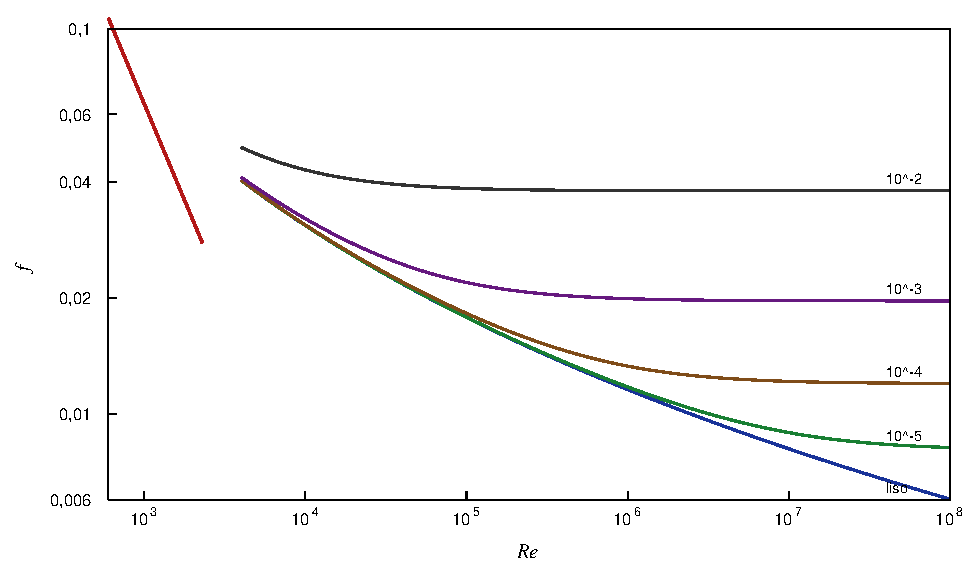
\includegraphics{../figures/FIG-0023/figure.pdf}}%
\count0=\ht0
\advance\count0 by \dp0
\count2=\wd0
\count4=\dimexpr\textheight/100*38\relax
\count6=\linewidth
\ifnum\count0<1
\count0=1
\fi
\ifnum\count2<1
\count2=1
\fi
\divide\count0 by 4096
\divide\count2 by 4096
\divide\count4 by 4096
\divide\count6 by 4096
\ifnum\count0<1
\count0=1
\fi
\ifnum\count2<1
\count2=1
\fi
\ifnum\count4<1
\count4=1
\fi
\ifnum\count6<1
\count6=1
\fi
\count8=\count2
\ifnum\count0>\count4
\count8=\numexpr\count2*\count4/\count0\relax
\fi
\ifnum\count8>\count6
\resizebox{\linewidth}{!}{\box0}%
\else
\ifnum\count0>\count4
\resizebox{!}{\dimexpr\textheight/100*38\relax}{\box0}%
\else
\box0%
\fi
\fi
\endgroup
\par\nopagebreak
\studiumcaption{fig:c10-moody}{Factor de fricción de Darcy frente al número de Reynolds: ley laminar \(64/\mathrm{Re}\) (hasta \(\mathrm{Re} = 2300\)) y aproximación de Haaland para rugosidades relativas \(\varepsilon/D = 0\), \(10^{-5}\), \(10^{-4}\), \(10^{-3}\) y \(10^{-2}\) (a partir de \(\mathrm{Re} = 4000\)). Curvas calculadas con las correlaciones, no datos experimentales.}
\end{minipage}
\par\vspace{\baselineskip}

\par\vspace{\baselineskip}
\noindent\begin{minipage}{\linewidth}
\centering
\begingroup
\setbox0=\hbox{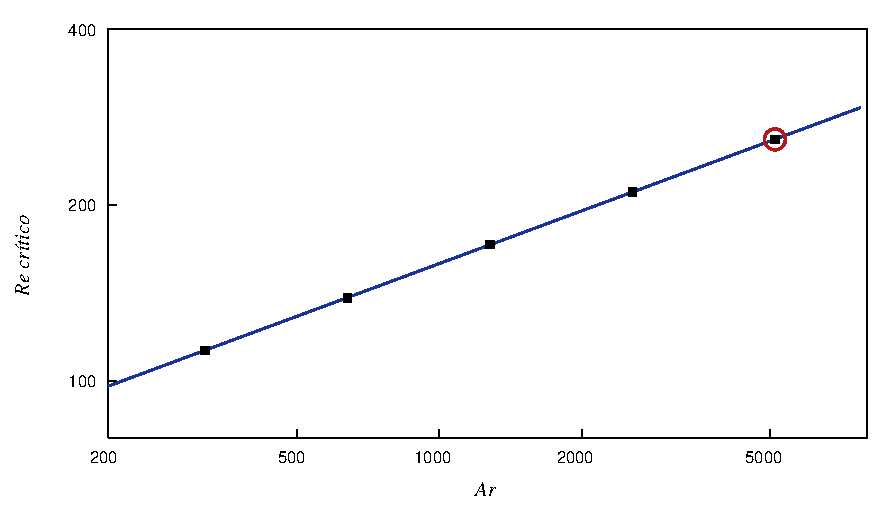
\includegraphics{../figures/FIG-0055/figure.pdf}}%
\count0=\ht0
\advance\count0 by \dp0
\count2=\wd0
\count4=\dimexpr\textheight/100*38\relax
\count6=\linewidth
\ifnum\count0<1
\count0=1
\fi
\ifnum\count2<1
\count2=1
\fi
\divide\count0 by 4096
\divide\count2 by 4096
\divide\count4 by 4096
\divide\count6 by 4096
\ifnum\count0<1
\count0=1
\fi
\ifnum\count2<1
\count2=1
\fi
\ifnum\count4<1
\count4=1
\fi
\ifnum\count6<1
\count6=1
\fi
\count8=\count2
\ifnum\count0>\count4
\count8=\numexpr\count2*\count4/\count0\relax
\fi
\ifnum\count8>\count6
\resizebox{\linewidth}{!}{\box0}%
\else
\ifnum\count0>\count4
\resizebox{!}{\dimexpr\textheight/100*38\relax}{\box0}%
\else
\box0%
\fi
\fi
\endgroup
\par\nopagebreak
\studiumcaption{fig:c10-flotabilidad}{Datos sintéticos de la tabla en variables adimensionales: número de Reynolds crítico frente al número de Arquímedes en escala doble logarítmica. Los puntos caen sobre una recta, \(\mathrm{Re}_c \propto \mathrm{Ar}^{0.30}\). El ensayo con boquilla de 8 mm y 10 N/m\(^3\) tiene \(\mathrm{Ar} = 5120\) y coincide con el último punto (círculo rojo).}
\end{minipage}
\par\vspace{\baselineskip}

\section{Teorema Pi de Buckingham}

El teorema Pi de Buckingham convierte la homogeneidad dimensional en un método. Si un fenómeno se describe mediante una relación entre \(n\) variables físicas en la que intervienen \(k\) dimensiones independientes, la relación puede reescribirse como una relación entre \(n - k\) grupos adimensionales independientes \(\Pi_1, \ldots, \Pi_{n-k}\) formados con esas variables; \(k\) es el rango de la matriz dimensional, cuyas columnas contienen los exponentes de \(M\), \(L\) y \(T\) de cada variable, y suele coincidir con el número de dimensiones básicas que aparecen. El fundamento es que una ley física no puede depender del sistema de unidades, de modo que debe poder expresarse solo con combinaciones adimensionales. El método de las variables repetidas permite construir los grupos: se eligen \(k\) variables que contengan entre todas las \(k\) dimensiones y no formen por sí solas un grupo adimensional, normalmente una densidad, una velocidad y una longitud; cada una de las variables restantes se combina con potencias de las repetidas, y los exponentes se obtienen imponiendo que la combinación sea adimensional. El teorema no dice qué grupos elegir: la elección no es única, y cualquier producto de potencias de grupos es otro grupo válido. La buena práctica consiste en escoger grupos con un significado físico claro, como cocientes de fuerzas o de escalas de tiempo.

Como ejemplo, la fuerza de resistencia \(F\) sobre una esfera lisa en un fluido incompresible depende de la densidad \(\rho\) y la viscosidad \(\mu\) del fluido, de la velocidad \(V\) y del diámetro \(d\). Son \(n = 5\) variables con \(k = 3\) dimensiones, de modo que bastan dos grupos. Con \(\rho\), \(V\) y \(d\) como variables repetidas, el primer grupo es \(\Pi_1 = F\rho^{a}V^{b}d^{c}\); imponiendo exponente nulo a la masa, a la longitud y al tiempo,
\begin{equation}
1 + a = 0,\qquad 1 - 3a + b + c = 0,\qquad -2 - b = 0, \label{eq:c10-exponentes}
\end{equation}
se obtiene \(a = -1\), \(b = -2\), \(c = -2\), es decir, \(\Pi_1 = F/(\rho V^{2} d^{2})\), que salvo un factor numérico es el coeficiente de resistencia. Repitiendo el procedimiento con la viscosidad resulta \(\Pi_2 = \mu/(\rho V d)\), el inverso del número de Reynolds. La relación buscada se reduce entonces a
\begin{equation}
C_D = \frac{F}{\tfrac12\rho V^{2}\,\pi d^{2}/4} = \Phi(\mathrm{Re}), \qquad \mathrm{Re} = \frac{\rho V d}{\mu}. \label{eq:c10-esfera}
\end{equation}
La reducción es enorme: en lugar de explorar experimentalmente cinco variables, basta medir una curva de \(C_D\) frente a \(\mathrm{Re}\) \emph{dentro de la familia física representada por las variables elegidas}: esferas lisas, flujo aproximadamente incompresible, fluidos newtonianos y ausencia de efectos adicionales relevantes como rugosidad, cavitación o rarefacción. No sirve sin más para cualquier fluido, tamaño o velocidad. Es exactamente la curva descrita en el capítulo 7, que incluye el régimen de Stokes, el de Newton y la crisis de la resistencia. El análisis dimensional no dice cuál es la función \(\Phi\), que debe medirse o calcularse, pero sí que no puede depender de nada más, si la lista inicial de variables era completa. Esa es la parte delicada del método: omitir una variable relevante, como la rugosidad o la compresibilidad, conduce a conclusiones erróneas.

\section{Grupos adimensionales y coeficientes aerodinámicos}

Los grupos adimensionales de la mecánica de fluidos tienen una interpretación física como cocientes entre fuerzas o entre escalas de tiempo. El número de Reynolds, \(\mathrm{Re} \equiv \rho V L/\mu\), o bien \(VL/\nu\), compara las fuerzas de inercia, del orden de \(\rho V^{2}/L\) por unidad de volumen, con las viscosas, del orden de \(\mu V/L^{2}\); es un parámetro fundamental del balance entre inercia y viscosidad, pero no determina por sí solo la transición laminar--turbulenta: también intervienen la geometría, las perturbaciones, la rugosidad y las condiciones de contorno. A números de Reynolds elevados, los efectos viscosos pueden concentrarse en capas límite, estelas y capas de mezcla, aunque no desaparecen del flujo. El número de Mach, \(\mathrm{Ma} \equiv V/a_s\), cociente entre la velocidad del flujo y la velocidad local del sonido, mide la importancia de la compresibilidad: por debajo de 0.3 el flujo puede tratarse como incompresible, entre 0.8 y 1.2 aparecen las dificultades del régimen transónico y por encima de 1, las ondas de choque. El número de Froude, \(\mathrm{Fr} \equiv V/\sqrt{gL}\), compara la inercia con la gravedad y gobierna los flujos con superficie libre, como las olas que genera un barco o el agua de un hidroavión al despegar. El número de Strouhal, introducido en el capítulo 8, mide la importancia de la no estacionariedad, y el número de Euler, \(\mathrm{Eu} \equiv \Delta p/(\rho V^{2})\), es la forma adimensional natural de las diferencias de presión. Los coeficientes aerodinámicos del capítulo 7 son grupos de este tipo: para un avión geométricamente definido, \(C_L\), \(C_D\) y el coeficiente de momento solo pueden depender del ángulo de ataque, del número de Reynolds y del de Mach, \(C_L = \Phi(\alpha, \mathrm{Re}, \mathrm{Ma})\). La figura~\ref{fig:c10-grupos} resume los grupos principales.

\section{Similaridad en flujos externos e internos}

Un modelo reproduce el comportamiento de un prototipo si existe semejanza geométrica, cinemática y dinámica. La semejanza geométrica exige que todas las longitudes estén en la misma proporción, incluidos detalles como la rugosidad superficial; la cinemática, que los campos de velocidad sean proporcionales; la dinámica, que las razones entre fuerzas sean iguales, lo que, por el teorema Pi, se consigue haciendo iguales en modelo y prototipo todos los grupos adimensionales independientes del problema. Si se cumple, los coeficientes medidos en el modelo son iguales a los del prototipo. El problema práctico es que rara vez pueden igualarse todos los grupos a la vez. Para igualar el número de Reynolds con el mismo fluido, la velocidad del modelo debe ser \(V_m = V_p(L_p/L_m)(\nu_m/\nu_p)\): un modelo a escala 1:10 ensayado en aire exigiría una velocidad diez veces mayor que la de vuelo, lo que alteraría el número de Mach. Un avión de negocios que se aproxima a 70 m/s con una cuerda media de 2.5 m opera a \(\mathrm{Re} = 1.225\cdot 70\cdot 2.5/1.7894\times 10^{-5} \approx 1.198\times 10^{7}\), imposible de reproducir en un túnel atmosférico convencional con un modelo pequeño. Las soluciones de ingeniería son los túneles presurizados, que aumentan la densidad, y los criogénicos, que con nitrógeno a baja temperatura aumentan la densidad y reducen la viscosidad a la vez; cuando ni siquiera así se alcanza el número de Reynolds de vuelo, se fija artificialmente la transición de la capa límite con bandas rugosas y se extrapolan los resultados.

El conflicto es aún más claro cuando intervienen la gravedad y la viscosidad. Con el mismo fluido y la misma gravedad, igualar el número de Froude exige \(V_m/V_p = \sqrt{L_m/L_p}\), mientras que igualar el de Reynolds exige \(V_m/V_p = L_p/L_m\); ambas condiciones solo son compatibles a escala natural. En los canales de ensayo de barcos y de flotadores de hidroaviones se iguala el número de Froude, que gobierna la resistencia por formación de olas, y la resistencia de fricción, que depende del número de Reynolds, se estima por separado con correlaciones de placa plana y se corrige: es el método propuesto por Froude en el siglo XIX, y sigue usándose. La lección general es que la semejanza completa es un ideal; la práctica consiste en identificar el grupo dominante para la magnitud que interesa, igualarlo, y corregir o acotar el efecto de los demás.

En flujos internos, el análisis dimensional de la caída de presión \(\Delta p\) en un tramo recto de longitud \(L\) y diámetro \(D\), con rugosidad absoluta \(\varepsilon\), por el que circula un fluido de densidad \(\rho\) y viscosidad \(\mu\) con velocidad media \(V\), da siete variables y tres dimensiones, es decir, cuatro grupos: \(\Delta p/(\rho V^{2})\), \(L/D\), \(\mathrm{Re}\) y \(\varepsilon/D\). Como en flujo completamente desarrollado la caída de presión es proporcional a la longitud, se obtiene la ecuación de Darcy-Weisbach,
\begin{equation}
\Delta p = f_D\,\frac{L}{D}\,\frac{\rho V^{2}}{2}, \qquad f_D = \Phi\!\left(\mathrm{Re}, \frac{\varepsilon}{D}\right), \label{eq:c10-darcy}
\end{equation}
en la que toda la física está en el factor de fricción. En régimen laminar se recupera el resultado exacto del capítulo 6, \(f_D = 64/\mathrm{Re}\), independiente de la rugosidad. En régimen turbulento no hay solución exacta, y el factor de fricción procede de correlaciones ajustadas a experimentos, como la ecuación implícita de Colebrook-White, \(1/\sqrt{f} = -2\log_{10}[\varepsilon/(3.7D) + 2.51/(\mathrm{Re}\sqrt{f})]\), válida para \(\mathrm{Re} > 4000\), o su aproximación explícita de Haaland,
\begin{equation}
\frac{1}{\sqrt{f_D}} = -1.8\log_{10}\!\left[\left(\frac{\varepsilon/D}{3.7}\right)^{1.11} + \frac{6.9}{\mathrm{Re}}\right], \label{eq:c10-haaland}
\end{equation}
cuya discrepancia con los datos es del orden de la incertidumbre de estos. Para \(\mathrm{Re} = 10^{5}\) y una rugosidad relativa \(\varepsilon/D\) de \(10^{-4}\) da \(f_D \approx 0.01827\), frente a \(64/10^{5} = 0.00064\) que se obtendría, erróneamente, con la ley laminar. Estas correlaciones son relaciones empíricas, no leyes exactas, y el diagrama de Moody que las representa, reproducido de forma aproximada en la figura~\ref{fig:c10-moody}, es probablemente el gráfico más usado de la ingeniería de fluidos.

El teorema Pi es un procedimiento, y conviene aplicarlo siempre con los mismos pasos. Como ejemplo, consideremos un chorro de agua caliente que se inyecta verticalmente hacia arriba, por una boquilla de diámetro \(d\), en un depósito de agua fría en reposo. Por debajo de cierta velocidad el chorro es laminar y estable; por encima, empieza a oscilar y acaba siendo turbulento. Se quiere saber de qué depende esa velocidad crítica \(U_c\). Paso 1: enumerar las variables. Además de \(U_c\) y \(d\), intervienen la viscosidad \(\mu\) y la densidad \(\rho\) del agua, que controlan la inercia y la difusión de cantidad de movimiento, y la flotabilidad, que en un chorro solo actúa a través de la diferencia de peso específico entre el chorro y el medio, \(\Delta(\rho g)\), en N/m\(^3\); la gravedad y las dos densidades no aparecen por separado si la diferencia de densidad es pequeña. Paso 2: dimensiones. \(U_c\) [L T\(^{-1}\)], \(d\) [L], \(\mu\) [M L\(^{-1}\)T\(^{-1}\)], \(\rho\) [M L\(^{-3}\)], \(\Delta(\rho g)\) [M L\(^{-2}\)T\(^{-2}\)]. Paso 3: contar. Hay \(n = 5\) variables y \(k = 3\) dimensiones independientes, luego \(5 - 3 = 2\) grupos. Paso 4: elegir las variables repetidas. Deben ser \(k = 3\), contener entre todas M, L y T, no poder formar por sí solas un grupo adimensional y no incluir la variable que se quiere determinar, para que esta aparezca en un único grupo. Elegimos \(\rho\), \(\mu\) y \(d\); elegir \(U_c\) entre ellas sería legítimo, pero poco práctico: la incógnita quedaría repartida entre los dos grupos y la relación entre ellos sería implícita.

Paso 5: formar los grupos combinando cada variable restante con las repetidas. Para \(U_c\) resulta el número de Reynolds del chorro, \(\Pi_1 = \rho U_c d/\mu = \mathrm{Re}\). Para la flotabilidad se escribe \(\Pi_2 = \Delta(\rho g)\,\rho^{a}\mu^{b}d^{c}\) y se exige que sea adimensional: la masa da \(1 + a + b = 0\), el tiempo \(-2 - b = 0\) y la longitud \(-2 - 3a - b + c = 0\), cuya solución es \(a = 1\), \(b = -2\), \(c = 3\):
\begin{equation}
\Pi_2 = \frac{\rho\,\Delta(\rho g)\,d^{3}}{\mu^{2}} = \mathrm{Ar}, \label{eq:c10-arquimedes}
\end{equation}
el número de Arquímedes, cociente entre las fuerzas de flotabilidad y las viscosas. Paso 6: escribir la relación, \(\mathrm{Re}_c = \Phi(\mathrm{Ar})\), y comprobar que cada grupo es realmente adimensional. La función \(\Phi\) no la da el análisis dimensional: hay que medirla. Lo que sí da el análisis es un resultado muy fuerte: dos ensayos con el mismo número de Arquímedes tienen el mismo número de Reynolds crítico, sean cuales sean por separado su diámetro, su viscosidad o su flotabilidad.

Los grupos no son únicos: cualquier producto de potencias de \(\mathrm{Re}\) y \(\mathrm{Ar}\) es también adimensional. El número de Richardson densimétrico, \(\mathrm{Ri} = \Delta(\rho g)\,d/(\rho U^{2})\), compara la flotabilidad con la inercia y cumple \(\mathrm{Ri} = \mathrm{Ar}/\mathrm{Re}^{2}\); su inversa, con raíz cuadrada, es el número de Froude densimétrico, \(U/\sqrt{g' d}\), con la gravedad reducida \(g' = \Delta(\rho g)/\rho\). Cuando la diferencia de densidad procede de una diferencia de temperatura \(\Delta T\), \(\Delta\rho \approx \rho\beta\Delta T\) y el número de Arquímedes se convierte en el de Grashof, \(g\beta\Delta T L^{3}/\nu^{2}\), que gobierna la convección natural. ¿Qué pareja conviene usar? La que deja la incógnita en un solo grupo. \(\mathrm{Re}\) y \(\mathrm{Ar}\) son la elección natural porque \(\mathrm{Ar}\) no contiene \(U_c\): se puede calcular antes de conocer la respuesta y fija el punto de operación. Con \(\mathrm{Re}\) y \(\mathrm{Ri}\), la incógnita aparecería en ambos grupos y la predicción exigiría resolver una ecuación implícita.

Ejemplo con datos. En una serie de ensayos con una boquilla de 4.0 mm de diámetro y agua de viscosidad 1.0 mPa s y densidad 1000 kg/m\(^3\) se mide la velocidad crítica para varias flotabilidades. Los datos de la tabla son sintéticos, generados para este ejercicio con una correlación del tipo \(\mathrm{Re}_c = C\,\mathrm{Ar}^{n}\); no son medidas publicadas.
\[
\begin{array}{c|ccccc}
\Delta(\rho g)\ (\mathrm{N/m^{3}}) & 5 & 10 & 20 & 40 & 80 \\ \hline
U_c\ (\mathrm{mm/s}) & 28.2 & 34.7 & 42.8 & 52.7 & 64.8 \\
\mathrm{Ar} & 320 & 640 & 1280 & 2560 & 5120
\end{array}
\]
Se pide la velocidad crítica de un segundo ensayo con el mismo líquido, una boquilla de 8.0 mm y \(\Delta(\rho g) = 10\) N/m\(^3\). La tentación es interpolar en la columna de 10 N/m\(^3\), pero esa columna corresponde a otro diámetro. Lo correcto es calcular el número de Arquímedes del nuevo ensayo, \(1000\cdot 10\cdot 0.008^3/(1.0\times 10^{-3})^2 = 5120\), y observar que coincide con el del ensayo a 80 N/m\(^3\), \(1000\cdot 80\cdot 0.004^3/(1.0\times 10^{-3})^2 = 5120\). Los dos ensayos son dinámicamente semejantes, sus números de Reynolds críticos coinciden y, con el mismo líquido, \(U_{c2} = U_{c1}\,d_1/d_2 = 64.8\cdot 0.004/0.008 = 32.4\) mm/s, sin interpolación alguna. En ese punto el número de Richardson vale \(80\cdot 0.004/(1000\cdot 0.0648^2) = 0.07621\), de modo que la inercia domina sobre la flotabilidad en la boquilla. La figura~\ref{fig:c10-flotabilidad} representa los datos en variables adimensionales.

La semejanza exacta solo es posible cuando el número de Arquímedes del ensayo nuevo coincide con uno medido. Si no coincide, por ejemplo con \(d = 4.0\) mm y \(\Delta(\rho g) = 30\) N/m\(^3\) (\(\mathrm{Ar} = 1920\)), hay que interpolar, y la regla es hacerlo en variables adimensionales y en la escala en que la relación es más regular, aquí logarítmica: entre los puntos de 20 y 40 N/m\(^3\) el exponente local es \(\log(52.7/42.8)/\log 2 \approx 0.30\), y \(U_c \approx 42.8\cdot(30/20)^{0.30} = 48.34\) mm/s. Interpolar es legítimo cuando el punto está dentro del intervalo medido y la curva es suave; extrapolar fuera de él, o interpolar en una variable dimensional entre ensayos con distinto diámetro o viscosidad, no lo es. En los ensayos con modelos el razonamiento se invierte: para reproducir a escala \(\lambda = d_m/d_p\) un chorro real con el mismo fluido hay que igualar \(\mathrm{Ar}\), lo que exige \(\Delta(\rho g)_m = \Delta(\rho g)_p/\lambda^{3}\), y entonces la igualdad de \(\mathrm{Re}\) fija \(U_m = U_p/\lambda\). Si no se puede ajustar la flotabilidad, hay que cambiar de fluido para modificar \(\mu\) y \(\rho\): la semejanza restringe a la vez la velocidad, la longitud, la densidad, la viscosidad y la flotabilidad.

\begin{tcolorbox}[title={Consejo}, studiumtip, breakable]

Antes de aplicar el teorema Pi, escriba la lista completa de variables y la matriz dimensional, y compruebe su rango: el número de dimensiones independientes no siempre coincide con el número de dimensiones que aparecen. Después compruebe que cada grupo obtenido es realmente adimensional; un error en un exponente se detecta así de inmediato.

Ante una tabla experimental y un ensayo modificado, calcule primero los grupos adimensionales independientes del ensayo nuevo. Si coinciden con los de un punto medido, la respuesta sale por semejanza exacta; si caen entre dos puntos, interpole en variables adimensionales e indique la incertidumbre; si caen fuera, diga que el resultado es una extrapolación. Nunca interpole directamente en la columna dimensional de otra geometría.
\end{tcolorbox}

\begin{tcolorbox}[title={Definición}, studiumdef, breakable]

Semejanza dinámica: dos flujos geométricamente semejantes son dinámicamente semejantes cuando todos los grupos adimensionales independientes que gobiernan el fenómeno, obtenidos con el teorema Pi de Buckingham, toman los mismos valores en ambos. Entonces los coeficientes adimensionales medidos en el modelo son válidos para el prototipo.
\end{tcolorbox}



\section{Desarrollos y práctica}

Las deducciones de este capítulo aplican el análisis dimensional \(\eqref{eq:c10-exponentes}\) a la resistencia de una esfera \(\eqref{eq:c10-esfera}\) y a la pérdida de carga en tubos \(\eqref{eq:c10-darcy}\), y muestran sus consecuencias para los ensayos en modelo: la velocidad necesaria para igualar el número de Reynolds y la imposibilidad de igualar simultáneamente los números de Froude y de Reynolds con el mismo fluido. La correlación de Haaland \(\eqref{eq:c10-haaland}\) completa la información necesaria para resolver problemas de tuberías en régimen turbulento. En los ejercicios, el primer paso es siempre enumerar las variables relevantes y sus dimensiones.

\begin{tcolorbox}[title={Desarrollos del modelo}, studiumdef, breakable]

\noindent\textbf{Grupos adimensionales de la resistencia de una esfera}

\[
F = \phi(\rho, V, d, \mu)\ \Rightarrow\ \frac{F}{\rho V^{2} d^{2}} = \Phi\!\left(\frac{\rho V d}{\mu}\right)
\]

\noindent\textbf{Hipótesis}
\begin{itemize}
\item la fuerza solo depende de rho, V, d y mu (sin compresibilidad ni superficie libre)
\item dimensiones fundamentales M, L, T (k = 3)
\end{itemize}

\noindent\textbf{Limitaciones}
\begin{itemize}
\item el análisis no da la forma de la función Phi: debe medirse o calcularse
\end{itemize}

\noindent\textbf{Pasos}
\begin{enumerate}
\item
n = 5 variables y k = 3 dimensiones: p = 2 grupos

\[
\Pi_1 = F\,\rho^{a} V^{b} d^{c}:\quad 1 + a = 0,\quad 1 - 3a + b + c = 0,\quad -2 - b = 0
\]
\item
elegir rho, V y d como variables repetidas

\[
a = -1,\ b = -2,\ c = -2\ \Rightarrow\ \Pi_1 = \frac{F}{\rho V^{2} d^{2}}
\]
\item
imponer exponentes nulos de M, L y T en F rho\(^a V^b d^c\)

\[
\Pi_2 = \frac{\mu}{\rho V d} = \mathrm{Re}^{-1}
\]
\item
relación usada en el texto (paso intermedio no comprobado por separado)

\[
\Pi_1 = F/(\rho V^{2} d^{2}),\qquad \Pi_2 = \mu/(\rho V d)
\]
\end{enumerate}

\noindent\textbf{Variables}
\begin{itemize}
\item $\Pi_{1}$: coeficiente de fuerza
\end{itemize}



\noindent\textbf{Ecuación de Darcy-Weisbach y su límite laminar}

\[
\Delta p = f_D\,\frac{L}{D}\,\frac{\rho V^{2}}{2},\qquad f_D = \Phi\!\left(\mathrm{Re}, \frac{\varepsilon}{D}\right)
\]

\noindent\textbf{Hipótesis}
\begin{itemize}
\item flujo completamente desarrollado en un conducto recto de sección constante
\end{itemize}

\noindent\textbf{Limitaciones}
\begin{itemize}
\item en régimen turbulento f depende de Re y de la rugosidad relativa a través de correlaciones empíricas
\end{itemize}

\noindent\textbf{Pasos}
\begin{enumerate}
\item
el teorema Pi con Delta p, L, D, V, rho, mu, epsilon da cuatro grupos

\[
\frac{\Delta p}{\rho V^{2}} = \Phi\!\left(\frac{L}{D}, \mathrm{Re}, \frac{\varepsilon}{D}\right)
\]
\item
la caída de presión es proporcional a L/D en flujo desarrollado

\[
f_D\,\frac{L}{D}\,\frac{\rho V^{2}}{2} = \frac{32\mu L V}{D^{2}}\ \Leftrightarrow\ f_D = \frac{64}{\mathrm{Re}}
\]
\item
en régimen laminar se recupera Hagen-Poiseuille con f = 64/Re
\end{enumerate}

\noindent\textbf{Variables}
\begin{itemize}
\item $\varepsilon$: rugosidad ($\mathrm{m}$)
\end{itemize}



\noindent\textbf{Velocidad de ensayo para igualar el número de Reynolds}

\begin{equation}
V_m = V_p\,\frac{L_p}{L_m}\,\frac{\nu_m}{\nu_p}
\label{eq:c10-semejanza}
\end{equation}

\noindent\textbf{Hipótesis}
\begin{itemize}
\item semejanza geométrica
\item el número de Reynolds es el único grupo relevante
\end{itemize}

\noindent\textbf{Limitaciones}
\begin{itemize}
\item si además importa el número de Mach o el de Froude, en general no pueden igualarse todos a la vez
\end{itemize}

\noindent\textbf{Pasos}
\begin{enumerate}
\item
igualar Re del modelo y del prototipo

\[
\frac{V_m L_m}{\nu_m} = \frac{V_p L_p}{\nu_p}
\]
\item
despejar la velocidad del modelo
\end{enumerate}

\noindent\textbf{Variables}
\begin{itemize}
\item $Lm$: longitud del modelo ($\mathrm{m}$)
\end{itemize}



\noindent\textbf{Incompatibilidad de la semejanza de Froude y de Reynolds con el mismo fluido}

\begin{equation}
\frac{V_m}{V_p} = \sqrt{\frac{L_m}{L_p}}\ \ (\mathrm{Fr}),\qquad \frac{V_m}{V_p} = \frac{L_p}{L_m}\ \ (\mathrm{Re}) \ \Rightarrow\ L_m = L_p
\label{eq:c10-froude-reynolds}
\end{equation}

\noindent\textbf{Hipótesis}
\begin{itemize}
\item mismo fluido y misma gravedad en modelo y prototipo
\end{itemize}

\noindent\textbf{Limitaciones}
\begin{itemize}
\item en ensayos navales se iguala Fr y se corrige la resistencia de fricción por separado
\end{itemize}

\noindent\textbf{Pasos}
\begin{enumerate}
\item
igualar Fr da la primera relación

\[
\frac{V_m}{\sqrt{g L_m}} = \frac{V_p}{\sqrt{g L_p}}
\]
\item
igualar Re con la misma viscosidad cinemática da la segunda

\[
\frac{V_m L_m}{\nu} = \frac{V_p L_p}{\nu}
\]
\item
ambas solo son compatibles a escala natural
\end{enumerate}

\noindent\textbf{Variables}
\begin{itemize}
\item $Lp$: longitud del prototipo ($\mathrm{m}$)
\end{itemize}



\noindent\textbf{Grupos adimensionales de un chorro con flotabilidad}

\begin{equation}
\frac{\rho U_c d}{\mu} = \Phi\!\left(\frac{\rho\,\Delta(\rho g)\,d^{3}}{\mu^{2}}\right),\qquad \mathrm{Ri} = \frac{\Delta(\rho g)\,d}{\rho U^{2}} = \frac{\mathrm{Ar}}{\mathrm{Re}^{2}}
\label{eq:c10-pi-flotabilidad}
\end{equation}

\noindent\textbf{Hipótesis}
\begin{itemize}
\item la velocidad crítica depende solo de d, mu, rho y Delta(rho g)
\item diferencias de densidad pequeñas (la densidad del chorro y del medio se representan por rho)
\end{itemize}

\noindent\textbf{Principios}
\begin{itemize}
\item homogeneidad dimensional
\item teorema Pi de Buckingham
\end{itemize}

\noindent\textbf{Aplicabilidad}
\begin{itemize}
\item chorros y plumas con flotabilidad en régimen laminar y de transición
\end{itemize}

\noindent\textbf{Limitaciones}
\begin{itemize}
\item la función Phi solo puede obtenerse experimentalmente
\item si la diferencia de densidad no es pequeña, el cociente de densidades es un tercer grupo
\end{itemize}

\noindent\textbf{Pasos}
\begin{enumerate}
\item
n = 5 variables, k = 3 dimensiones (M, L, T): 2 grupos

\[
1 + a + b = 0,\qquad -2 - b = 0,\qquad -2 - 3a - b + c = 0
\]
\item
variables repetidas rho, mu, d

\[
U_c = f\left(d,\ \mu,\ \rho,\ \Delta(\rho g)\right),\qquad 5 - 3 = 2
\]
\item
grupo de la incógnita U

\[
\Pi_1 = \frac{\rho U_c d}{\mu} = \mathrm{Re}
\]
\item
grupo de la flotabilidad: Delta(rho g) rho\(^a\) mu\(^b d^c\)

\[
\Pi_2 = \Delta(\rho g)\,\rho^{a}\mu^{b}d^{c}
\]
\item
exponentes: M 1 + a + b = 0, T -2 - b = 0, L -2 - 3a - b + c = 0

\[
a = 1,\qquad b = -2,\qquad c = 3
\]
\item

\[
\Pi_2 = \frac{\rho\,\Delta(\rho g)\,d^{3}}{\mu^{2}} = \mathrm{Ar}
\]
\end{enumerate}

\noindent\textbf{Variables}
\begin{itemize}
\item $d$: diámetro de la boquilla ($\mathrm{m}$)
\item $\Delta(\rho g)$: flotabilidad por unidad de volumen ($\mathrm{N}\,\mathrm{m}^{-3}$)
\end{itemize}



\noindent\textbf{Escalado de la velocidad crítica entre dos ensayos semejantes}

\begin{equation}
\mathrm{Ar}_2 = \mathrm{Ar}_1 \;\Rightarrow\; U_{c2} = U_{c1}\,\frac{\mu_2}{\mu_1}\,\frac{\rho_1}{\rho_2}\,\frac{d_1}{d_2}
\label{eq:c10-escalado-flotabilidad}
\end{equation}

\noindent\textbf{Hipótesis}
\begin{itemize}
\item la misma relación Re = Phi(Ar) vale para ambos ensayos (semejanza geométrica y del resto de condiciones)
\end{itemize}

\noindent\textbf{Principios}
\begin{itemize}
\item igualdad de los grupos independientes implica igualdad del grupo dependiente
\end{itemize}

\noindent\textbf{Limitaciones}
\begin{itemize}
\item si el número de Arquímedes del nuevo ensayo no coincide con ninguno medido, hay que interpolar en la curva Re(Ar)
\end{itemize}

\noindent\textbf{Pasos}
\begin{enumerate}
\item
si Ar coincide, Phi(Ar) coincide y por tanto Re coincide

\[
U_{c2} = U_{c1}\,\frac{\nu_2}{\nu_1}\,\frac{d_1}{d_2},\qquad \nu_i=\frac{\mu_i}{\rho_i}
\]
\item
despejar la velocidad de la igualdad de números de Reynolds

\[
\frac{\rho_2 U_{c2} d_2}{\mu_2} = \frac{\rho_1 U_{c1} d_1}{\mu_1}
\]
\item

\[
U_{c2} = U_{c1}\,\frac{\mu_2}{\mu_1}\,\frac{\rho_1}{\rho_2}\,\frac{d_1}{d_2}
\]
\end{enumerate}


\end{tcolorbox}

\begin{tcolorbox}[title={Problema resuelto}, studiumworked, breakable]

\noindent\textbf{Enunciado}
Se quiere ensayar a escala 1:10 el ala de un avión de negocios que se aproxima a 70 m/s con una cuerda media de 2.5 m, en aire a nivel del mar (\(\rho = 1.225\) kg/m\(^3\), \(\mu = 1.7894\times 10^{-5}\) Pa s). El túnel disponible alcanza 80 m/s y puede presurizarse manteniendo la temperatura. (a) Calcule el número de Reynolds de vuelo. (b) ¿Qué velocidad haría falta en un túnel atmosférico para igualarlo? (c) ¿A qué presión debe operar el túnel a 80 m/s? (d) Compare los números de Mach del modelo y del prototipo (\(a_s = 340\) m/s).

\noindent\textbf{Datos}
\begin{itemize}
\item $Vp = 70\,\mathrm{m}\,\mathrm{s}^{-1}$ — velocidad del prototipo
\item $Lp = 2.5\,\mathrm{m}$ — cuerda del prototipo
\item $Lm = 0.25\,\mathrm{m}$ — cuerda del modelo
\item $Vm = 80\,\mathrm{m}\,\mathrm{s}^{-1}$ — velocidad máxima del túnel
\item $p_{0} = 101325\,\mathrm{Pa}$ — presión atmosférica
\end{itemize}

\noindent\textbf{Incógnita}
presión de operación del túnel

\noindent\textbf{Modelo físico}

\noindent\textit{Igualdad de Reynolds con densidad proporcional a la presión}

\[
p_m = p_0\,\frac{V_p L_p}{V_m L_m}
\]

\noindent\textbf{Hipótesis}
\begin{itemize}
\item semejanza geométrica
\item temperatura igual en el túnel y en vuelo, de modo que la viscosidad no cambia
\item gas ideal: densidad proporcional a la presión
\end{itemize}

\noindent\textbf{Desarrollo paso a paso}

\phantomsection\label{solution:mf-010}
\noindent\textbf{Elección del procedimiento.} Con el mismo aire y temperatura, igualar Reynolds exige $\rho_mV_mL_m=\rho_pV_pL_p$. A presión atmosférica las densidades son iguales. Si se limita la velocidad, se eleva la densidad con la presión mediante el gas ideal a temperatura fija.

\begin{enumerate}

\item Calcular el Reynolds que se pretende reproducir.

\[\fitmath{\mathrm{Rep}=\frac{\rho\cdot \mathrm{Vp}\cdot \mathrm{Lp}}{\mu}}\]

\[\fitmath{\mathrm{Rep}=\frac{(1{,}225)\cdot (70)\cdot (2{,}5)}{(1{,}7894\times10^{-5})}\approx 1{,}198027\times10^{7}\,}\]

\item Cancelar densidad y viscosidad en ambos lados y despejar la velocidad del túnel atmosférico.

\[\fitmath{\mathrm{Vatm}=\frac{\mathrm{Vp}\cdot \mathrm{Lp}}{\mathrm{Lm}}}\]

\[\fitmath{\mathrm{Vatm}=\frac{(70)\cdot (2{,}5)}{(0{,}25)}\approx 700\,\mathrm{m/s}}\]

\item El Mach del ensayo limitado usa 80 m/s.

\[\fitmath{\mathrm{Mam}=\frac{\mathrm{Vm}}{\mathrm{asound}}}\]

\[\fitmath{\mathrm{Mam}=\frac{(80)}{(340)}\approx 0{,}2352941\,}\]

\item A temperatura fija $\rho_m/\rho_p=p_m/p_0$; despejar la presión absoluta de ensayo.

\[\fitmath{\mathrm{pm}=\frac{p_{0}\cdot \mathrm{Vp}\cdot \mathrm{Lp}}{\mathrm{Vm}\cdot \mathrm{Lm}}}\]

\[\fitmath{\mathrm{pm}=\frac{(101325)\cdot (70)\cdot (2{,}5)}{(80)\cdot (0{,}25)}\approx 886593{,}8\,\mathrm{Pa}}\]

\end{enumerate}


\noindent\textbf{Sustitución numérica}

\[
\frac{\left(2.5\,\mathrm{m}\right) \left(70\,\mathrm{m}\,\mathrm{s}^{-1}\right) \left(101325\,\mathrm{Pa}\right)}{\left(0.25\,\mathrm{m}\right) \left(80\,\mathrm{m}\,\mathrm{s}^{-1}\right)}
\]

\noindent\textbf{Resultado}

\[
\mathrm{Re} \approx 1.2\times 10^{7},\quad V_{\mathrm{atm}} = 700\ \mathrm{m/s},\quad p_m \approx 8.9\times 10^{5}\ \mathrm{Pa}\ (8.75\ \mathrm{atm})
\]

\noindent\textbf{Interpretación}
Un túnel atmosférico necesitaría flujo supersónico para igualar \(\mathrm{Re}\), lo que destruiría la semejanza de Mach. Al presurizar hasta casi 9 atm y mantener la temperatura se iguala el número de Reynolds, pero \emph{no} el número de Mach: \(\mathrm{Ma}_m=80/340\approx0.235\) frente a \(\mathrm{Ma}_p=70/340\approx0.206\), una discrepancia relativa cercana al 14 \%. Para este ejemplo subsónico de Mach pequeño puede admitirse una aproximación de flujo incompresible, pero no debe afirmarse una similitud dinámica exacta en ambos números.

\noindent\textbf{Comprobación de la respuesta} la aritmética del último paso reproduce la respuesta enunciada a la precisión con que está escrita. Es una reproducción aritmética; no valida el modelo físico ni sus hipótesis.

\noindent\textbf{Limitaciones}
\begin{itemize}
\item las cargas sobre el modelo crecen con la presión dinámica, casi nueve veces mayor
\item pequeñas diferencias de temperatura cambian la viscosidad
\end{itemize}

\noindent\textbf{Errores frecuentes}
\begin{itemize}
\item igualar la velocidad en lugar del número de Reynolds
\item olvidar que a temperatura constante la viscosidad no cambia con la presión
\end{itemize}
\end{tcolorbox}

\begin{tcolorbox}[title={Ejercicios propuestos}, studiumworked, breakable]

\noindent\textbf{1 (Básico, DIMENSIONAL)}
La caída de presión en un tramo recto de tubería depende de \(\Delta p\), \(L\), \(D\), \(V\), \(\rho\), \(\mu\) y \(\varepsilon\). ¿Cuántos grupos adimensionales independientes intervienen? Proponga un conjunto con significado físico.

\noindent\textbf{2 (Intermedio, Cálculo)}
Un avión de transporte vuela a 230 m/s a 11 km, donde \(\rho = 0.36392\) kg/m\(^3\) y \(T = 216.65\) K. Con la ley de Sutherland (\(\mu_0 = 1.716\times 10^{-5}\) Pa s, \(T_0 = 273.15\) K, \(S = 110.4\) K) calcule la viscosidad, el número de Reynolds basado en una cuerda de 4.0 m y el número de Mach (\(\gamma = 1.4\), \(R_a = 287.05\) J/(kg K)).

\noindent\textbf{3 (Intermedio, Aplicación)}
Se ensaya en un canal un modelo a escala 1:50 del flotador de un hidroavión anfibio grande que se desplaza a 10 m/s en el agua. Con semejanza de Froude, ¿a qué velocidad debe remolcarse el modelo?

\noindent\textbf{4 (De examen, Desarrollo)}
El empuje de una hélice depende de \(\rho\), \(V\), \(n\) (revoluciones por segundo), \(D\) y \(\mu\). (a) Demuestre que \(C_T = T/(\rho n^{2}D^{4})\) es función del grado de avance \(J = V/(nD)\) y del número de Reynolds. (b) En un ensayo con un modelo se mide \(C_T = 0.10\) para \(J = 0.6\). Suponiendo efecto de Reynolds despreciable, estime el empuje de una hélice semejante de 2.5 m de diámetro que gira a 40 rev/s en aire a nivel del mar (\(\rho = 1.225\) kg/m\(^3\)) con el mismo \(J\).

\noindent\textbf{5 (Avanzado, Desarrollo)}
Por una tubería de acero comercial de 100 mm de diámetro (\(\varepsilon = 0.045\) mm) circula agua a 20 \(^\circ\)C (\(\rho = 998.2\) kg/m\(^3\), \(\nu = 1.007\times 10^{-6}\) m\(^2\)/s) con velocidad media de 1.0 m/s. Calcule el número de Reynolds, el factor de fricción con la ecuación de Haaland y la caída de presión en 100 m.

\noindent\textbf{6 (Básico, DIMENSIONAL)}
Para el chorro con flotabilidad del texto, con \(\rho = 1000\) kg/m\(^3\), \(\mu = 1.0\times 10^{-3}\) Pa s, \(d = 4.0\) mm y \(\Delta(\rho g) = 40\) N/m\(^3\): (a) compruebe por análisis dimensional que \(\rho\,\Delta(\rho g)\,d^{3}/\mu^{2}\) es adimensional; (b) calcule su valor.

\noindent\textbf{7 (Intermedio, Aplicación)}
Con la tabla de ensayos del texto (\(d = 4.0\) mm, agua con \(\mu = 1.0\) mPa s y \(\rho = 1000\) kg/m\(^3\)), determine sin interpolar la velocidad crítica de un chorro del mismo líquido con boquilla de 8.0 mm y \(\Delta(\rho g) = 10\) N/m\(^3\).

\noindent\textbf{8 (Avanzado, Desarrollo)}
Se repite el ensayo con una mezcla de agua y glicerina de la misma densidad (1000 kg/m\(^3\), aproximación) pero viscosidad 2.0 mPa s, con la boquilla de 4.0 mm. (a) ¿Qué flotabilidad \(\Delta(\rho g)\) hay que imponer para que el ensayo sea semejante al de la tabla con 20 N/m\(^3\)? (b) ¿Cuál será su velocidad crítica?

\noindent\textbf{9 (De examen, Interpretación)}
Con la misma tabla, un ensayo con \(d = 4.0\) mm, agua (\(\mu = 1.0\) mPa s, \(\rho = 1000\) kg/m\(^3\)) y \(\Delta(\rho g) = 30\) N/m\(^3\): (a) calcule su número de Arquímedes y explique por qué no se puede resolver por semejanza exacta con los datos disponibles; (b) estime la velocidad crítica interpolando en escala logarítmica entre los dos ensayos más próximos; (c) calcule el número de Richardson en la boquilla y comente qué fuerza domina; (d) indique qué ensayo adicional, con el mismo líquido y \(\Delta(\rho g) = 240\) N/m\(^3\), permitiría evitar la interpolación y con qué diámetro.
\end{tcolorbox}

\begin{tcolorbox}[title={Autoevaluación}, studiumcheck, breakable]

(1) ¿Por qué una ecuación dimensionalmente homogénea puede ser falsa? (2) La potencia de una hélice depende de \(\rho\), \(V\), \(n\) (revoluciones por segundo), \(D\) y \(\mu\): ¿cuántos grupos adimensionales hay y cuáles elegiría? (3) ¿Qué ocurre si en un análisis dimensional se omite una variable relevante? (4) ¿Por qué un túnel criogénico permite alcanzar números de Reynolds más altos que uno atmosférico del mismo tamaño? (5) ¿Por qué en los ensayos de barcos se iguala el número de Froude y no el de Reynolds? (6) ¿Depende el factor de fricción laminar de la rugosidad? ¿Y el turbulento a número de Reynolds muy alto?

(1) ¿Cuántos grupos adimensionales tiene un problema con \(n\) variables y \(k\) dimensiones independientes? (2) ¿Por qué no debe incluirse la incógnita entre las variables repetidas? (3) Deduzca los exponentes del número de Arquímedes. (4) Demuestre que \(\mathrm{Ri} = \mathrm{Ar}/\mathrm{Re}^{2}\). (5) ¿Por qué un ensayo con boquilla de 8 mm y 10 N/m\(^3\) es semejante a otro con boquilla de 4 mm y 80 N/m\(^3\)? (6) ¿Cuándo es legítimo interpolar en una tabla experimental?
\end{tcolorbox}
\studiumchaptercheck

\part{Tema 5. Ampliación del formalismo matemático y aplicaciones}

\chapter{Operadores diferenciales e integrales}
\label{chap:c11}

\studiumchapterguide{Las leyes de conservación de la mecánica de fluidos pueden escribirse de dos maneras equivalentes: como balances integrales sobre volúmenes finitos, como en el capítulo 9, o como ecuaciones diferenciales que valen en cada punto. El puente entre ambas son los operadores diferenciales vectoriales y los teoremas integrales de Gauss y de Stokes. La guía docente dedica a este formalismo la primera parte del Tema 5. Este capítulo repasa el gradiente, la divergencia, el rotacional y el laplaciano con su interpretación física en un campo de velocidades, define el flujo y la circulación, y presenta los teoremas de Gauss, Stokes y Helmholtz, que serán imprescindibles para deducir la ecuación de continuidad, introducir la vorticidad y el potencial de velocidad, y obtener las ecuaciones de Navier-Stokes.}

\section{Gradiente, divergencia, rotacional y laplaciano}

El operador nabla, que en coordenadas cartesianas es \(\nabla = \mathbf{i}\,\partial/\partial x + \mathbf{j}\,\partial/\partial y + \mathbf{k}\,\partial/\partial z\), genera los tres operadores diferenciales de primer orden. Aplicado a un campo escalar \(f\) da su gradiente, \(\nabla f\), un vector que apunta en la dirección de máximo crecimiento de \(f\) y cuyo módulo es la tasa de crecimiento en esa dirección. La derivada de \(f\) en la dirección de un vector unitario \(\mathbf{e}\) es \(\mathbf{e}\cdot\nabla f\), y la variación de \(f\) entre dos puntos próximos es \(df = \nabla f\cdot d\mathbf{x}\); por eso el gradiente es perpendicular a las superficies de nivel \(f = \mathrm{cte}\). Ya han aparecido dos gradientes con significado físico: en el capítulo 1, la fuerza conservativa \(-\nabla E_p\), y en el capítulo 5, la fuerza neta de presión por unidad de volumen \(-\nabla p\), que empuja el fluido de las zonas de alta presión hacia las de baja. La divergencia del gradiente es el laplaciano, \(\nabla^{2}f = \partial^{2}f/\partial x^{2} + \partial^{2}f/\partial y^{2} + \partial^{2}f/\partial z^{2}\), que mide cuánto se aparta el valor de \(f\) en un punto del valor medio de \(f\) en una pequeña esfera a su alrededor. Por eso aparece en todos los procesos de difusión, que tienden a suavizar las diferencias: en la conducción del calor, en la difusión de masa y, como se verá, en la difusión viscosa de la cantidad de movimiento.

\par\vspace{\baselineskip}
\noindent\begin{minipage}{\linewidth}
\centering
\begingroup
\setbox0=\hbox{\begin{tikzpicture}
\shade[ball color=blue!15,opacity=0.6] (0,0) ellipse (3 and 1.1);
\draw[thick,blue!60!black] (0,0) ellipse (3 and 1.1);
\draw[->,very thick,red] (2.12,0.78) arc (40:80:3 and 1.1);
\node[red] at (2.4,1.2) {$d\mathbf{l}$};
\draw[->,thick] (0,0) -- (0,2.0) node[above]{$\mathbf{n}$};
\draw[->,teal,thick] (-1.2,-0.3) -- (-1.0,1.4) node[above]{\small $\nabla\times\mathbf{u}$};
\draw[->,teal,thick] (1.1,-0.4) -- (1.3,1.2);
\node at (2.9,-0.9) {$C$}; \node at (-0.6,-0.5) {$S$};
\end{tikzpicture}}%
\count0=\ht0
\advance\count0 by \dp0
\count2=\wd0
\count4=\dimexpr\textheight/100*38\relax
\count6=\linewidth
\ifnum\count0<1
\count0=1
\fi
\ifnum\count2<1
\count2=1
\fi
\divide\count0 by 4096
\divide\count2 by 4096
\divide\count4 by 4096
\divide\count6 by 4096
\ifnum\count0<1
\count0=1
\fi
\ifnum\count2<1
\count2=1
\fi
\ifnum\count4<1
\count4=1
\fi
\ifnum\count6<1
\count6=1
\fi
\count8=\count2
\ifnum\count0>\count4
\count8=\numexpr\count2*\count4/\count0\relax
\fi
\ifnum\count8>\count6
\resizebox{\linewidth}{!}{\begin{tikzpicture}
\shade[ball color=blue!15,opacity=0.6] (0,0) ellipse (3 and 1.1);
\draw[thick,blue!60!black] (0,0) ellipse (3 and 1.1);
\draw[->,very thick,red] (2.12,0.78) arc (40:80:3 and 1.1);
\node[red] at (2.4,1.2) {$d\mathbf{l}$};
\draw[->,thick] (0,0) -- (0,2.0) node[above]{$\mathbf{n}$};
\draw[->,teal,thick] (-1.2,-0.3) -- (-1.0,1.4) node[above]{\small $\nabla\times\mathbf{u}$};
\draw[->,teal,thick] (1.1,-0.4) -- (1.3,1.2);
\node at (2.9,-0.9) {$C$}; \node at (-0.6,-0.5) {$S$};
\end{tikzpicture}}%
\else
\ifnum\count0>\count4
\resizebox{!}{\dimexpr\textheight/100*38\relax}{\begin{tikzpicture}
\shade[ball color=blue!15,opacity=0.6] (0,0) ellipse (3 and 1.1);
\draw[thick,blue!60!black] (0,0) ellipse (3 and 1.1);
\draw[->,very thick,red] (2.12,0.78) arc (40:80:3 and 1.1);
\node[red] at (2.4,1.2) {$d\mathbf{l}$};
\draw[->,thick] (0,0) -- (0,2.0) node[above]{$\mathbf{n}$};
\draw[->,teal,thick] (-1.2,-0.3) -- (-1.0,1.4) node[above]{\small $\nabla\times\mathbf{u}$};
\draw[->,teal,thick] (1.1,-0.4) -- (1.3,1.2);
\node at (2.9,-0.9) {$C$}; \node at (-0.6,-0.5) {$S$};
\end{tikzpicture}}%
\else
\begin{tikzpicture}
\shade[ball color=blue!15,opacity=0.6] (0,0) ellipse (3 and 1.1);
\draw[thick,blue!60!black] (0,0) ellipse (3 and 1.1);
\draw[->,very thick,red] (2.12,0.78) arc (40:80:3 and 1.1);
\node[red] at (2.4,1.2) {$d\mathbf{l}$};
\draw[->,thick] (0,0) -- (0,2.0) node[above]{$\mathbf{n}$};
\draw[->,teal,thick] (-1.2,-0.3) -- (-1.0,1.4) node[above]{\small $\nabla\times\mathbf{u}$};
\draw[->,teal,thick] (1.1,-0.4) -- (1.3,1.2);
\node at (2.9,-0.9) {$C$}; \node at (-0.6,-0.5) {$S$};
\end{tikzpicture}%
\fi
\fi
\endgroup
\par\nopagebreak
\studiumcaption{fig:c11-stokes}{Teorema de Stokes: la circulación de la velocidad a lo largo de la curva cerrada \(C\) es igual al flujo de la vorticidad \(\nabla\times\mathbf{u}\) a través de cualquier superficie \(S\) apoyada en \(C\), con la normal \(\mathbf{n}\) orientada según la regla de la mano derecha.}
\end{minipage}
\par\vspace{\baselineskip}

\par\vspace{\baselineskip}
\noindent\begin{minipage}{\linewidth}
\centering
\begingroup
\setbox0=\hbox{\begin{tikzpicture}
\draw[->] (0,0) -- (8.2,0) node[right]{$r/a$};
\draw[->] (0,0) -- (0,3.6) node[above]{$u_\theta/u_{\theta,\max}$};
\draw[very thick,blue] (0,0) -- (1,3);
\draw[very thick,blue,domain=1:8,samples=80] plot (\x,{3/\x});
\draw[dashed] (1,0) node[below]{$1$} -- (1,3);
\draw[dashed] (0,3) node[left]{$1$} -- (1,3);
\node[below] at (4,0) {$4$}; \node[below] at (8,0) {$8$};
\node at (0.3,3.3) {\scriptsize núcleo};
\node at (4.5,1.2) {\small $u_\theta = \Gamma_C/(2\pi r)$};
\end{tikzpicture}}%
\count0=\ht0
\advance\count0 by \dp0
\count2=\wd0
\count4=\dimexpr\textheight/100*38\relax
\count6=\linewidth
\ifnum\count0<1
\count0=1
\fi
\ifnum\count2<1
\count2=1
\fi
\divide\count0 by 4096
\divide\count2 by 4096
\divide\count4 by 4096
\divide\count6 by 4096
\ifnum\count0<1
\count0=1
\fi
\ifnum\count2<1
\count2=1
\fi
\ifnum\count4<1
\count4=1
\fi
\ifnum\count6<1
\count6=1
\fi
\count8=\count2
\ifnum\count0>\count4
\count8=\numexpr\count2*\count4/\count0\relax
\fi
\ifnum\count8>\count6
\resizebox{\linewidth}{!}{\begin{tikzpicture}
\draw[->] (0,0) -- (8.2,0) node[right]{$r/a$};
\draw[->] (0,0) -- (0,3.6) node[above]{$u_\theta/u_{\theta,\max}$};
\draw[very thick,blue] (0,0) -- (1,3);
\draw[very thick,blue,domain=1:8,samples=80] plot (\x,{3/\x});
\draw[dashed] (1,0) node[below]{$1$} -- (1,3);
\draw[dashed] (0,3) node[left]{$1$} -- (1,3);
\node[below] at (4,0) {$4$}; \node[below] at (8,0) {$8$};
\node at (0.3,3.3) {\scriptsize núcleo};
\node at (4.5,1.2) {\small $u_\theta = \Gamma_C/(2\pi r)$};
\end{tikzpicture}}%
\else
\ifnum\count0>\count4
\resizebox{!}{\dimexpr\textheight/100*38\relax}{\begin{tikzpicture}
\draw[->] (0,0) -- (8.2,0) node[right]{$r/a$};
\draw[->] (0,0) -- (0,3.6) node[above]{$u_\theta/u_{\theta,\max}$};
\draw[very thick,blue] (0,0) -- (1,3);
\draw[very thick,blue,domain=1:8,samples=80] plot (\x,{3/\x});
\draw[dashed] (1,0) node[below]{$1$} -- (1,3);
\draw[dashed] (0,3) node[left]{$1$} -- (1,3);
\node[below] at (4,0) {$4$}; \node[below] at (8,0) {$8$};
\node at (0.3,3.3) {\scriptsize núcleo};
\node at (4.5,1.2) {\small $u_\theta = \Gamma_C/(2\pi r)$};
\end{tikzpicture}}%
\else
\begin{tikzpicture}
\draw[->] (0,0) -- (8.2,0) node[right]{$r/a$};
\draw[->] (0,0) -- (0,3.6) node[above]{$u_\theta/u_{\theta,\max}$};
\draw[very thick,blue] (0,0) -- (1,3);
\draw[very thick,blue,domain=1:8,samples=80] plot (\x,{3/\x});
\draw[dashed] (1,0) node[below]{$1$} -- (1,3);
\draw[dashed] (0,3) node[left]{$1$} -- (1,3);
\node[below] at (4,0) {$4$}; \node[below] at (8,0) {$8$};
\node at (0.3,3.3) {\scriptsize núcleo};
\node at (4.5,1.2) {\small $u_\theta = \Gamma_C/(2\pi r)$};
\end{tikzpicture}%
\fi
\fi
\endgroup
\par\nopagebreak
\studiumcaption{fig:c11-rankine}{Velocidad tangencial del torbellino de Rankine con circulación \(\Gamma_C\) y núcleo de radio \(a\): crecimiento lineal dentro del núcleo (rotación rígida, vorticidad uniforme) y decrecimiento como \(\tfrac{1}{r}\) fuera (torbellino libre, irrotacional).}
\end{minipage}
\par\vspace{\baselineskip}

La divergencia de un campo vectorial, \(\nabla\cdot\mathbf{u} = \partial u/\partial x + \partial v/\partial y + \partial w/\partial z\), es un escalar con una interpretación cinemática precisa cuando \(\mathbf{u}\) es la velocidad de un fluido. Consideremos un paralelepípedo material infinitesimal de aristas \(\delta x\), \(\delta y\), \(\delta z\). En un tiempo \(dt\), la arista paralela al eje \(x\) se alarga porque su extremo derecho se mueve más deprisa que el izquierdo en \((\partial u/\partial x)\,\delta x\), de modo que su longitud se multiplica por \(1 + (\partial u/\partial x)\,dt\), y análogamente las otras dos. El volumen se multiplica por el producto de los tres factores, y en el límite \(dt \to 0\),
\begin{equation}
\frac{1}{\delta V}\frac{D(\delta V)}{Dt} = \nabla\cdot\mathbf{u}. \label{eq:c11-dilatacion}
\end{equation}
La divergencia de la velocidad es, por tanto, la tasa de expansión volumétrica relativa de las partículas de fluido: positiva cuando el fluido se expande, como el aire que se calienta, y negativa cuando se comprime. Un flujo incompresible, en el que cada partícula conserva su volumen, tiene divergencia nula, que es la forma diferencial de la condición de incompresibilidad anunciada en el capítulo 4 y que el capítulo 12 deducirá de la conservación de la masa. Un campo de divergencia nula se llama solenoidal.

El rotacional de un campo vectorial, \(\nabla\times\mathbf{u}\), mide su densidad de circulación local: su componente según una dirección \(\mathbf{n}\) es el límite de la circulación de \(\mathbf{u}\) a lo largo de una pequeña curva perpendicular a \(\mathbf{n}\) dividida por el área que encierra. Cuando \(\mathbf{u}\) es la velocidad, su rotacional es la vorticidad, \(\boldsymbol{\omega} = \nabla\times\mathbf{u}\), y es igual al doble de la velocidad angular local con que giran las partículas de fluido. Para comprobarlo basta tomar la rotación como sólido rígido \(\mathbf{u} = \boldsymbol{\Omega}\times\mathbf{x}\), que con \(\boldsymbol{\Omega} = \Omega\mathbf{k}\) es \(\mathbf{u} = (-\Omega y, \Omega x, 0)\):
\begin{equation}
\omega_z = \frac{\partial v}{\partial x} - \frac{\partial u}{\partial y} = 2\Omega, \qquad \nabla\cdot\mathbf{u} = 0. \label{eq:c11-rigido}
\end{equation}
Un campo de rotacional nulo se llama irrotacional. Rotación del flujo y vorticidad no son lo mismo: en el torbellino libre \(u_\theta = K/(2\pi r)\) las partículas describen circunferencias alrededor del eje (la figura~\ref{fig:c11-rankine} muestra este campo fuera del núcleo de un torbellino real), pero, como \(r u_\theta\) es constante, la vorticidad \(\omega_z = (1/r)\,d(r u_\theta)/dr\) es nula en todos los puntos salvo en el eje; cada partícula recorre su órbita sin girar sobre sí misma, como la cabina de una noria. Al contrario, en el flujo cortante \(u = \dot\gamma y\), con líneas de corriente rectas, la vorticidad es \(-\dot\gamma\), no nula: las partículas giran mientras se trasladan en línea recta. Las identidades \(\nabla\times(\nabla f) = \mathbf{0}\) y \(\nabla\cdot(\nabla\times\mathbf{A}) = 0\), válidas para campos suficientemente derivables, tienen consecuencias físicas directas: un campo que es gradiente de un potencial es irrotacional, y la vorticidad, al ser un rotacional, es solenoidal.

\section{Flujo y circulación}

Dos integrales de un campo vectorial aparecen continuamente en mecánica de fluidos. El flujo de un campo \(\mathbf{F}\) a través de una superficie \(S\) con normal unitaria \(\mathbf{n}\) es la integral de su componente normal, \(\iint_S \mathbf{F}\cdot\mathbf{n}\,dS\). Si \(\mathbf{F}\) es la velocidad, el flujo es el caudal volumétrico que atraviesa la superficie, \(Q = \iint_S \mathbf{u}\cdot\mathbf{n}\,dS\); si es \(\rho\mathbf{u}\), el gasto másico; si es \(\rho\mathbf{u}(\mathbf{u}\cdot\mathbf{n})\), el flujo de cantidad de movimiento que se usó en el capítulo 9. Por ejemplo, el caudal de un perfil parabólico \(u = U_{\max}(1 - r^{2}/R^{2})\) en un tubo es \(\int_0^{R} U_{\max}(1 - r^{2}/R^{2})\,2\pi r\,dr = \pi R^{2}U_{\max}/2\), resultado ya obtenido en el capítulo 6 y comprobado aquí simbólicamente. La circulación a lo largo de una curva cerrada \(C\) es la integral de línea de la componente tangencial de la velocidad,
\begin{equation}
\Gamma_C = \oint_C \mathbf{u}\cdot d\mathbf{l}. \label{eq:c11-circulacion}
\end{equation}
Introducida por Kelvin como medida cinemática del movimiento de rotación de un fluido, la circulación desempeña un papel central en aerodinámica: el teorema de Kutta-Joukowski, que se verá en el capítulo 12, establece que la sustentación por unidad de envergadura de un perfil es \(\rho V_\infty\Gamma_C\), donde \(\Gamma_C\) es la circulación alrededor del perfil. En el torbellino libre, la circulación a lo largo de cualquier circunferencia centrada vale \(\int_0^{2\pi}(K/2\pi r)\,r\,d\theta = K\), independiente del radio, lo que identifica el parámetro \(K\) como la intensidad del torbellino.

\section{Teoremas de Gauss, Stokes y Helmholtz}

El teorema de la divergencia, o de Gauss, afirma que el flujo saliente de un campo vectorial derivable \(\mathbf{F}\) a través de una superficie cerrada \(S\) es igual a la integral de su divergencia en el volumen \(V\) que encierra,
\begin{equation}
\iint_S \mathbf{F}\cdot\mathbf{n}\,dS = \iiint_V \nabla\cdot\mathbf{F}\,dV. \label{eq:c11-gauss}
\end{equation}
Intuitivamente, la suma de todas las fuentes del campo dentro de una región, contando los sumideros como fuentes negativas, es el flujo neto que sale de ella. Como ilustración, para \(\mathbf{F} = \mathbf{x}\) y una esfera de radio \(R\), la divergencia vale 3 y su integral es \(3\cdot\tfrac43\pi R^{3} = 4\pi R^{3}\), mientras que sobre la superficie \(\mathbf{F}\cdot\mathbf{n} = R\) y el flujo es \(R\cdot 4\pi R^{2}\), el mismo valor. Su importancia en mecánica de fluidos es que permite transformar los balances integrales sobre volúmenes de control en ecuaciones diferenciales locales: si un balance de la forma \(\iiint_V (\ldots)\,dV + \iint_S (\ldots)\cdot\mathbf{n}\,dS\) se anula para cualquier volumen, el teorema de Gauss convierte la integral de superficie en una de volumen y, como el volumen es arbitrario, el integrando debe anularse en cada punto. Así se obtendrán la ecuación de continuidad en el capítulo 12 y la de cantidad de movimiento en el capítulo 14. Existen versiones del teorema para campos escalares, \(\iint_S f\,\mathbf{n}\,dS = \iiint_V \nabla f\,dV\), y tensoriales, que se usan para transformar la fuerza de presión y la de los esfuerzos viscosos.

El teorema de Stokes relaciona la circulación de un campo a lo largo de una curva cerrada \(C\) con el flujo de su rotacional a través de cualquier superficie \(S\) que se apoye en ella, con la orientación dada por la regla de la mano derecha,
\begin{equation}
\oint_C \mathbf{F}\cdot d\mathbf{l} = \iint_S (\nabla\times\mathbf{F})\cdot\mathbf{n}\,dS. \label{eq:c11-stokes}
\end{equation}
Aplicado a la velocidad, dice que la circulación a lo largo de una curva es el flujo de vorticidad que la atraviesa. En la rotación rígida, la circulación sobre una circunferencia de radio \(R\) es \(\Omega R\cdot 2\pi R\) y el flujo de la vorticidad uniforme \(2\Omega\) sobre el círculo es \(2\Omega\cdot\pi R^{2}\): ambos valen \(2\pi\Omega R^{2}\). La figura~\ref{fig:c11-stokes} ilustra el teorema. Una consecuencia inmediata es que en una región simplemente conexa donde el flujo es irrotacional la circulación sobre cualquier curva cerrada es nula, y la velocidad puede escribirse como gradiente de un potencial, \(\mathbf{u} = \nabla\phi\). Esta conclusión falla en regiones múltiplemente conexas, como el exterior de un perfil: el flujo puede ser irrotacional en todo el fluido y tener circulación no nula alrededor del perfil, precisamente la que produce sustentación. Finalmente, el teorema de descomposición de Helmholtz afirma que todo campo vectorial suficientemente regular que decae en el infinito puede escribirse como la suma de un campo irrotacional y uno solenoidal, \(\mathbf{u} = \nabla\phi + \nabla\times\mathbf{A}_v\). En mecánica de fluidos, la parte irrotacional describe la expansión y la solenoidal, la rotación; para flujos planos incompresibles, el potencial vector se reduce a la función de corriente del capítulo 12.

\begin{tcolorbox}[title={Consejo}, studiumtip, breakable]

No confunda flujo con trayectorias circulares con flujo rotacional: la vorticidad es una propiedad local, que mide el giro de cada partícula sobre sí misma, no la curvatura de su trayectoria. Calcule siempre \(\nabla\times\mathbf{u}\) antes de afirmar que un flujo es irrotacional.
\end{tcolorbox}

\begin{tcolorbox}[title={Definición}, studiumdef, breakable]

Circulación \(\Gamma_C\): integral de línea de la componente tangencial de la velocidad a lo largo de una curva cerrada. Por el teorema de Stokes es igual al flujo de la vorticidad a través de cualquier superficie apoyada en la curva, de modo que un campo irrotacional tiene circulación nula alrededor de toda curva reducible a un punto.
\end{tcolorbox}



\section{Desarrollos y práctica}

Las deducciones que siguen dan significado físico a los operadores diferenciales: la divergencia como tasa de dilatación \(\eqref{eq:c11-dilatacion}\), el rotacional de la rotación como sólido rígido \(\eqref{eq:c11-rigido}\), la circulación del torbellino libre \(\eqref{eq:c11-circulacion}\), y la comprobación directa de los teoremas de Gauss \(\eqref{eq:c11-gauss}\) y de Stokes \(\eqref{eq:c11-stokes}\). Estos resultados son las herramientas con las que el capítulo 12 pasará de las leyes integrales a las diferenciales. En los ejercicios conviene comprobar el resultado calculando las dos integrales de cada teorema por separado.

\begin{tcolorbox}[title={Desarrollos del modelo}, studiumdef, breakable]

\noindent\textbf{La divergencia de la velocidad como tasa de dilatación volumétrica}

\[
\frac{1}{\delta V}\frac{D(\delta V)}{Dt} = \nabla\cdot\mathbf{u} = \frac{\partial u}{\partial x} + \frac{\partial v}{\partial y} + \frac{\partial w}{\partial z}
\]

\noindent\textbf{Hipótesis}
\begin{itemize}
\item paralelepípedo material infinitesimal de aristas paralelas a los ejes
\item campo de velocidad derivable
\end{itemize}

\noindent\textbf{Limitaciones}
\begin{itemize}
\item es una propiedad local: para volúmenes finitos se usa el teorema de Gauss
\end{itemize}

\noindent\textbf{Pasos}
\begin{enumerate}
\item
en un tiempo dt cada arista se alarga en proporción a la derivada de la componente de velocidad correspondiente

\[
\delta V(t + dt) = \delta x\,\delta y\,\delta z\,(1 + a\,dt)(1 + b\,dt)(1 + c\,dt)
\]
\item
el volumen se multiplica por el producto de los tres factores

\[
\lim_{dt\to 0}\frac{(1 + a\,dt)(1 + b\,dt)(1 + c\,dt) - 1}{dt} = a + b + c
\]
\item
se toma el límite dt tendiendo a cero
\end{enumerate}

\noindent\textbf{Variables}
\begin{itemize}
\item $a$: derivada parcial de u respecto a x ($\mathrm{1/s}$)
\end{itemize}



\noindent\textbf{Vorticidad de la rotación como sólido rígido}

\[
\mathbf{u} = \boldsymbol{\Omega}\times\mathbf{x} = (-\Omega y,\ \Omega x,\ 0)\ \Rightarrow\ \nabla\times\mathbf{u} = 2\boldsymbol{\Omega},\quad \nabla\cdot\mathbf{u} = 0
\]

\noindent\textbf{Hipótesis}
\begin{itemize}
\item rotación uniforme alrededor del eje z
\end{itemize}

\noindent\textbf{Limitaciones}
\begin{itemize}
\item la vorticidad es el doble de la velocidad angular local de rotación de las partículas
\end{itemize}

\noindent\textbf{Pasos}
\begin{enumerate}
\item
calcular la componente z del rotacional

\[
\omega_z = \frac{\partial v}{\partial x} - \frac{\partial u}{\partial y} = \Omega - (-\Omega) = 2\Omega
\]
\item
calcular la divergencia

\[
\nabla\cdot\mathbf{u} = \frac{\partial(-\Omega y)}{\partial x} + \frac{\partial(\Omega x)}{\partial y} = 0
\]
\end{enumerate}

\noindent\textbf{Variables}
\begin{itemize}
\item $\Omega$: velocidad angular ($\mathrm{rad}\,\mathrm{s}^{-1}$)
\end{itemize}



\noindent\textbf{Torbellino libre: campo irrotacional con circulación constante}

\begin{equation}
u_\theta = \frac{K}{2\pi r}\ \Rightarrow\ \omega_z = \frac{1}{r}\frac{d(r u_\theta)}{dr} = 0\ (r > 0),\qquad \Gamma_C = \oint u_\theta\,r\,d\theta = K
\label{eq:c11-torbellino}
\end{equation}

\noindent\textbf{Hipótesis}
\begin{itemize}
\item flujo plano con líneas de corriente circulares
\item velocidad solo función del radio
\end{itemize}

\noindent\textbf{Limitaciones}
\begin{itemize}
\item la velocidad diverge en el eje: un torbellino real tiene un núcleo con vorticidad
\end{itemize}

\noindent\textbf{Pasos}
\begin{enumerate}
\item
la componente axial del rotacional en polares es \((1/r) d(r u_theta)/dr\)

\[
\omega_z = \frac{1}{r}\frac{d}{dr}\left(\frac{K}{2\pi}\right) = 0
\]
\item
\(r u_theta\) es constante, luego el rotacional es nulo fuera del eje

\[
\Gamma_C = \int_0^{2\pi}\frac{K}{2\pi r}\,r\,d\theta = K
\]
\item
la circulación sobre cualquier circunferencia centrada vale K

\[
u_\theta = K/(2\pi r)
\]
\item
relación usada en el texto (paso intermedio no comprobado por separado)

\[
\omega_z = (1/r)\,d(r u_\theta)/dr
\]
\item
relación usada en el texto (paso intermedio no comprobado por separado)
\end{enumerate}

\noindent\textbf{Variables}
\begin{itemize}
\item $K$: intensidad del torbellino ($\mathrm{m}^{2}\,\mathrm{s}^{-1}$)
\end{itemize}



\noindent\textbf{Comprobación del teorema de Gauss en una esfera}

\[
\iiint_V \nabla\cdot\mathbf{F}\,dV = \iint_S \mathbf{F}\cdot\mathbf{n}\,dS:\qquad \mathbf{F} = \mathbf{x},\ \ 3\cdot\tfrac43\pi R^{3} = R\cdot 4\pi R^{2}
\]

\noindent\textbf{Hipótesis}
\begin{itemize}
\item campo F = x (posición), esfera de radio R centrada en el origen
\end{itemize}

\noindent\textbf{Limitaciones}
\begin{itemize}
\item un ejemplo no demuestra el teorema; ilustra su contenido
\end{itemize}

\noindent\textbf{Pasos}
\begin{enumerate}
\item
la divergencia de x es 3 en todo punto

\[
\iiint_V 3\,dV = 4\pi R^{3}
\]
\item
sobre la esfera, \(x \cdot n = R\)

\[
\iint_S R\,dS = 4\pi R^{3}
\]
\item
ambas integrales valen 4 pi \(R^3\)
\end{enumerate}

\noindent\textbf{Variables}
\begin{itemize}
\item $R$: radio de la esfera ($\mathrm{m}$)
\end{itemize}



\noindent\textbf{Comprobación del teorema de Stokes en la rotación rígida}

\[
\oint_C \mathbf{u}\cdot d\mathbf{l} = \iint_S (\nabla\times\mathbf{u})\cdot\mathbf{n}\,dS:\qquad (\Omega R)(2\pi R) = (2\Omega)(\pi R^{2})
\]

\noindent\textbf{Hipótesis}
\begin{itemize}
\item rotación rígida con velocidad angular Omega
\item C circunferencia de radio R centrada en el eje
\end{itemize}

\noindent\textbf{Limitaciones}
\begin{itemize}
\item ilustración del teorema en un caso particular
\end{itemize}

\noindent\textbf{Pasos}
\begin{enumerate}
\item
la velocidad tangencial en C es Omega R

\[
\Gamma_C = \Omega R\cdot 2\pi R = 2\pi\Omega R^{2}
\]
\item
la vorticidad es uniforme e igual a 2 Omega

\[
\iint_S 2\Omega\,dS = 2\pi\Omega R^{2}
\]
\end{enumerate}

\noindent\textbf{Variables}
\begin{itemize}
\item $W$: velocidad angular ($\mathrm{rad}\,\mathrm{s}^{-1}$)
\end{itemize}


\end{tcolorbox}

\begin{tcolorbox}[title={Problema resuelto}, studiumworked, breakable]

\noindent\textbf{Enunciado}
El torbellino de punta de ala que deja un avión de transporte en aproximación tiene una circulación de 400 m\(^2\)/s. Modélelo como un torbellino de Rankine: rotación como sólido rígido dentro de un núcleo de 3.0 m de radio y torbellino libre fuera de él, con velocidad continua en el borde del núcleo. Calcule la vorticidad en el núcleo, la velocidad tangencial máxima y la velocidad a 30 m del eje. Comente el riesgo para un avión ligero que lo atraviese.

\noindent\textbf{Datos}
\begin{itemize}
\item $\Gamma = 400\,\mathrm{m}^{2}\,\mathrm{s}^{-1}$ — circulación del torbellino
\item $a = 3.0\,\mathrm{m}$ — radio del núcleo
\item $r = 30\,\mathrm{m}$ — distancia de interés
\end{itemize}

\noindent\textbf{Incógnita}
velocidad tangencial máxima

\noindent\textbf{Modelo físico}

\noindent\textit{Velocidad en el borde del núcleo de Rankine}

\[
u_{\theta,\max} = \frac{\Gamma_C}{2\pi a}
\]

\noindent\textbf{Hipótesis}
\begin{itemize}
\item torbellino plano y estacionario
\item vorticidad uniforme en el núcleo y nula fuera de él
\end{itemize}

\noindent\textbf{Desarrollo paso a paso}

\phantomsection\label{solution:mf-011}
\noindent\textbf{Elección del procedimiento.} En el núcleo $u_\theta=\Omega r$ y fuera $u_\theta=\Gamma/(2\pi r)$. La continuidad en $r=a$ fija $\Omega=\Gamma/(2\pi a^2)$. La vorticidad del giro rígido es $2\Omega$. La velocidad crece dentro y decrece fuera, por eso el máximo está en el borde.

\begin{enumerate}

\item Igualar las velocidades interior y exterior en el radio del núcleo.

\[\fitmath{\Omega=\frac{\Gamma}{2\cdot \pi\cdot {a}^{2}}}\]

\[\fitmath{\Omega=\frac{(400)}{2\cdot \pi\cdot {(3)}^{2}}\approx 7.073553\,\mathrm{1/s}}\]

\item La vorticidad es el doble de la velocidad angular del giro rígido.

\[\fitmath{\mathrm{wz}=2\cdot \Omega}\]

\[\fitmath{\mathrm{wz}=2\cdot (7.073553026)\approx 14.14711\,\mathrm{1/s}}\]

\item Evaluar la velocidad en el borde.

\[\fitmath{\mathrm{umax}=\Omega\cdot a}\]

\[\fitmath{\mathrm{umax}=(7.073553026)\cdot (3)\approx 21.22066\,\mathrm{m/s}}\]

\item Como 30 m supera 3 m, usar la rama exterior.

\[\fitmath{\mathrm{ur}=\frac{\Gamma}{2\cdot \pi\cdot r}}\]

\[\fitmath{\mathrm{ur}=\frac{(400)}{2\cdot \pi\cdot (30)}\approx 2.122066\,\mathrm{m/s}}\]

\end{enumerate}


\noindent\textbf{Sustitución numérica}

\[
\frac{\left(400\,\mathrm{m}^{2}\,\mathrm{s}^{-1}\right)}{2 \pi \left(3.0\,\mathrm{m}\right)}
\]

\noindent\textbf{Resultado}

\[
\omega \approx 14.1\ \mathrm{s^{-1}},\quad u_{\theta,\max} \approx 21.2\ \mathrm{m/s},\quad u_\theta(30\ \mathrm{m}) \approx 2.12\ \mathrm{m/s}
\]

\noindent\textbf{Interpretación}
Una velocidad tangencial de 21 m/s en un radio de pocos metros puede inducir en un avión ligero un balance mayor que el que pueden compensar sus alerones: de ahí las separaciones mínimas por estela turbulenta entre aviones.

\noindent\textbf{Comprobación de la respuesta} la aritmética del último paso reproduce la respuesta enunciada a la precisión con que está escrita. Es una reproducción aritmética; no valida el modelo físico ni sus hipótesis.

\noindent\textbf{Limitaciones}
\begin{itemize}
\item los torbellinos reales tienen perfiles de velocidad suaves y decaen con el tiempo
\item la circulación real depende del peso, la velocidad y la envergadura del avión generador
\end{itemize}

\noindent\textbf{Errores frecuentes}
\begin{itemize}
\item usar la fórmula del torbellino libre dentro del núcleo, donde daría velocidades infinitas
\end{itemize}
\end{tcolorbox}

\begin{tcolorbox}[title={Ejercicios propuestos}, studiumworked, breakable]

\noindent\textbf{1 (Intermedio, Cálculo)}
En la capa de aceite de un cojinete el flujo es aproximadamente \(u = \dot\gamma y\), \(v = 0\), con \(\dot\gamma = 100\) s\(^{-1}\). Calcule la componente \(z\) de la vorticidad.

\noindent\textbf{2 (Intermedio, Cálculo)}
Calcule el caudal que atraviesa la sección de un tubo de 0.10 m de diámetro con un perfil de velocidad \(u = U_{\max}(1 - r^{2}/R^{2})\) y \(U_{\max} = 2.0\) m/s, integrando el flujo de la velocidad.

\noindent\textbf{3 (Avanzado, Desarrollo)}
Un depósito cilíndrico de combustible gira como un sólido rígido a 3.0 rad/s. Calcule la circulación a lo largo de una circunferencia de 0.40 m de radio centrada en el eje de dos maneras: directamente y mediante el teorema de Stokes.

\noindent\textbf{4 (De examen, Desarrollo)}
En una región de gas que se calienta uniformemente, la velocidad es \(\mathbf{u} = k\,\mathbf{x}\) con \(k = 0.10\) s\(^{-1}\). Use el teorema de Gauss para calcular el caudal volumétrico neto que sale de una esfera de 2.0 m de radio centrada en el origen, y compruébelo calculando el flujo directamente.

\noindent\textbf{5 (Básico, Cálculo)}
Calcule la divergencia del campo de velocidades \(\mathbf{u} = (2x,\ -3y,\ z)\) s\(^{-1}\) y diga si puede representar el flujo de un fluido incompresible.
\end{tcolorbox}

\begin{tcolorbox}[title={Autoevaluación}, studiumcheck, breakable]

(1) ¿Qué significa físicamente que la divergencia de la velocidad sea positiva en una región? (2) Calcule la vorticidad del flujo cortante \(u = \dot\gamma y\), \(v = 0\), y explique por qué no es nula aunque las líneas de corriente sean rectas. (3) ¿Por qué el torbellino libre es irrotacional y sin embargo tiene circulación no nula? (4) Use el teorema de Gauss para demostrar que el caudal neto que sale de cualquier superficie cerrada en un flujo incompresible es nulo. (5) ¿Por qué no se puede asegurar que un flujo irrotacional alrededor de un perfil derive de un potencial monovaluado? (6) ¿Qué relación hay entre el laplaciano y los procesos de difusión?
\end{tcolorbox}
\studiumchaptercheck

\chapter{Transporte de Reynolds, continuidad y flujo potencial}
\label{chap:c12}

\studiumchapterguide{Este capítulo reúne los resultados centrales del Tema 5: el teorema del transporte de Reynolds, que generaliza el método del volumen de control del capítulo 9; la ecuación de continuidad, forma local de la conservación de la masa; la función de corriente y la vorticidad, que describen de forma compacta los flujos planos; el flujo potencial, que permite resolver con métodos lineales el flujo de un fluido ideal alrededor de cuerpos; y la ecuación de Bernoulli, probablemente la relación más usada y peor aplicada de la mecánica de fluidos. El objetivo es que el lector sepa no solo usar estos resultados, sino también reconocer las hipótesis en que se apoyan y, por tanto, cuándo dejan de valer.}

\section{Teorema del transporte de Reynolds}

Las leyes de conservación se enuncian para sistemas, pero los análisis de ingeniería se hacen en volúmenes de control. Sea \(B\) una propiedad extensiva del fluido, como la masa, la cantidad de movimiento o la energía, y \(\beta \equiv dB/dm\) su valor por unidad de masa, de modo que la cantidad de \(B\) contenida en un volumen es \(\int \rho\beta\,dV\). Consideremos un volumen de control fijo \(VC\) con superficie \(SC\) y el sistema que en el instante \(t\) ocupa exactamente ese volumen. La derivada temporal de \(B\) en el sistema difiere de la derivada de \(B\) contenida en el volumen de control por dos razones: el contenido del volumen de control puede cambiar con el tiempo, y en un instante \(dt\) parte del sistema sale del volumen de control mientras entra fluido que no pertenece al sistema. Contabilizando ambos efectos se obtiene el teorema del transporte de Reynolds,
\begin{equation}
\frac{dB_{\mathrm{sis}}}{dt} = \frac{\partial}{\partial t}\int_{VC}\rho\beta\,dV + \int_{SC}\rho\beta\,(\mathbf{u}\cdot\mathbf{n})\,dA, \label{eq:c12-rtt}
\end{equation}
donde \(\mathbf{n}\) es la normal exterior: el producto \(\rho\,(\mathbf{u}\cdot\mathbf{n})\,dA\) es el gasto másico que atraviesa el elemento de superficie, positivo hacia fuera y negativo hacia dentro. Si el volumen de control se mueve con velocidad uniforme, basta sustituir \(\mathbf{u}\) por la velocidad relativa a él. El teorema es una generalización tridimensional de la regla de Leibniz para derivar una integral con límites variables, y es puramente cinemático: no contiene ninguna ley física. Su potencia está en que, sustituyendo \(B\) por la masa, la cantidad de movimiento o la energía e igualando el primer miembro a lo que dicta la ley física correspondiente, se obtienen las ecuaciones integrales de conservación en volúmenes de control. Los balances del capítulo 9 son sus casos particulares estacionarios con entradas y salidas uniformes, como muestra la figura~\ref{fig:c12-rtt}.

\par\vspace{\baselineskip}
\noindent\begin{minipage}{\linewidth}
\centering
\begingroup
\setbox0=\hbox{\begin{tikzpicture}
\draw[very thick] (0,0) rectangle (4,2.4);
\fill[gray!25] (0,0) rectangle (4,2.4);
\draw[thick,dashed,red] (0.7,0) rectangle (4.7,2.4);
\fill[blue!20] (0,0) rectangle (0.7,2.4); \node at (0.35,1.2) {I};
\fill[orange!30] (4,0) rectangle (4.7,2.4); \node at (4.35,1.2) {II};
\draw[->,thick] (-1.2,1.2) -- (-0.1,1.2) node[midway,above]{$\mathbf{u}$};
\draw[->,thick] (4.8,1.2) -- (5.9,1.2);
\node at (2.2,1.2) {VC};
\node[red] at (2.7,2.75) {sistema en $t + dt$};
\node at (2.0,-0.35) {sistema en $t$ = VC};
\end{tikzpicture}}%
\count0=\ht0
\advance\count0 by \dp0
\count2=\wd0
\count4=\dimexpr\textheight/100*38\relax
\count6=\linewidth
\ifnum\count0<1
\count0=1
\fi
\ifnum\count2<1
\count2=1
\fi
\divide\count0 by 4096
\divide\count2 by 4096
\divide\count4 by 4096
\divide\count6 by 4096
\ifnum\count0<1
\count0=1
\fi
\ifnum\count2<1
\count2=1
\fi
\ifnum\count4<1
\count4=1
\fi
\ifnum\count6<1
\count6=1
\fi
\count8=\count2
\ifnum\count0>\count4
\count8=\numexpr\count2*\count4/\count0\relax
\fi
\ifnum\count8>\count6
\resizebox{\linewidth}{!}{\begin{tikzpicture}
\draw[very thick] (0,0) rectangle (4,2.4);
\fill[gray!25] (0,0) rectangle (4,2.4);
\draw[thick,dashed,red] (0.7,0) rectangle (4.7,2.4);
\fill[blue!20] (0,0) rectangle (0.7,2.4); \node at (0.35,1.2) {I};
\fill[orange!30] (4,0) rectangle (4.7,2.4); \node at (4.35,1.2) {II};
\draw[->,thick] (-1.2,1.2) -- (-0.1,1.2) node[midway,above]{$\mathbf{u}$};
\draw[->,thick] (4.8,1.2) -- (5.9,1.2);
\node at (2.2,1.2) {VC};
\node[red] at (2.7,2.75) {sistema en $t + dt$};
\node at (2.0,-0.35) {sistema en $t$ = VC};
\end{tikzpicture}}%
\else
\ifnum\count0>\count4
\resizebox{!}{\dimexpr\textheight/100*38\relax}{\begin{tikzpicture}
\draw[very thick] (0,0) rectangle (4,2.4);
\fill[gray!25] (0,0) rectangle (4,2.4);
\draw[thick,dashed,red] (0.7,0) rectangle (4.7,2.4);
\fill[blue!20] (0,0) rectangle (0.7,2.4); \node at (0.35,1.2) {I};
\fill[orange!30] (4,0) rectangle (4.7,2.4); \node at (4.35,1.2) {II};
\draw[->,thick] (-1.2,1.2) -- (-0.1,1.2) node[midway,above]{$\mathbf{u}$};
\draw[->,thick] (4.8,1.2) -- (5.9,1.2);
\node at (2.2,1.2) {VC};
\node[red] at (2.7,2.75) {sistema en $t + dt$};
\node at (2.0,-0.35) {sistema en $t$ = VC};
\end{tikzpicture}}%
\else
\begin{tikzpicture}
\draw[very thick] (0,0) rectangle (4,2.4);
\fill[gray!25] (0,0) rectangle (4,2.4);
\draw[thick,dashed,red] (0.7,0) rectangle (4.7,2.4);
\fill[blue!20] (0,0) rectangle (0.7,2.4); \node at (0.35,1.2) {I};
\fill[orange!30] (4,0) rectangle (4.7,2.4); \node at (4.35,1.2) {II};
\draw[->,thick] (-1.2,1.2) -- (-0.1,1.2) node[midway,above]{$\mathbf{u}$};
\draw[->,thick] (4.8,1.2) -- (5.9,1.2);
\node at (2.2,1.2) {VC};
\node[red] at (2.7,2.75) {sistema en $t + dt$};
\node at (2.0,-0.35) {sistema en $t$ = VC};
\end{tikzpicture}%
\fi
\fi
\endgroup
\par\nopagebreak
\studiumcaption{fig:c12-rtt}{Teorema del transporte de Reynolds: volumen de control fijo (línea continua) y sistema que coincide con él en el instante \(t\) (gris) y se ha desplazado en \(t + dt\) (línea discontinua). La diferencia entre ambos se debe al flujo saliente (región II) y entrante (región I) a través de la superficie de control.}
\end{minipage}
\par\vspace{\baselineskip}

\par\vspace{\baselineskip}
\noindent\begin{minipage}{\linewidth}
\centering
\begingroup
\setbox0=\hbox{\begin{tikzpicture}
% studium:potential-cylinder-v2
\fill[gray!35] (0,0) circle (1);
\draw[thick] (0,0) circle (1);
\draw[blue,thick,->] (-4.5,0) -- (-1,0);
\draw[blue,thick,->] (1,0) -- (4.5,0);
\draw[blue,smooth] plot coordinates {(-4.50000,0.21037) (-4.41000,0.21082) (-4.32000,0.21129) (-4.23000,0.21181) (-4.14000,0.21236) (-4.05000,0.21295) (-3.96000,0.21358) (-3.87000,0.21426) (-3.78000,0.21500) (-3.69000,0.21579) (-3.60000,0.21666) (-3.51000,0.21759) (-3.42000,0.21861) (-3.33000,0.21973) (-3.24000,0.22095) (-3.15000,0.22229) (-3.06000,0.22377) (-2.97000,0.22541) (-2.88000,0.22723) (-2.79000,0.22925) (-2.70000,0.23153) (-2.61000,0.23409) (-2.52000,0.23699) (-2.43000,0.24030) (-2.34000,0.24410) (-2.25000,0.24849) (-2.16000,0.25362) (-2.07000,0.25966) (-1.98000,0.26685) (-1.89000,0.27553) (-1.80000,0.28614) (-1.71000,0.29932) (-1.62000,0.31599) (-1.53000,0.33748) (-1.44000,0.36566) (-1.35000,0.40306) (-1.26000,0.45243) (-1.17000,0.51526) (-1.08000,0.58933) (-0.99000,0.66846) (-0.90000,0.74590) (-0.81000,0.81726) (-0.72000,0.88060) (-0.63000,0.93544) (-0.54000,0.98193) (-0.45000,1.02043) (-0.36000,1.05134) (-0.27000,1.07502) (-0.18000,1.09173) (-0.09000,1.10168) (0.00000,1.10499) (0.09000,1.10168) (0.18000,1.09173) (0.27000,1.07502) (0.36000,1.05134) (0.45000,1.02043) (0.54000,0.98193) (0.63000,0.93544) (0.72000,0.88060) (0.81000,0.81726) (0.90000,0.74590) (0.99000,0.66846) (1.08000,0.58933) (1.17000,0.51526) (1.26000,0.45243) (1.35000,0.40306) (1.44000,0.36566) (1.53000,0.33748) (1.62000,0.31599) (1.71000,0.29932) (1.80000,0.28614) (1.89000,0.27553) (1.98000,0.26685) (2.07000,0.25966) (2.16000,0.25362) (2.25000,0.24849) (2.34000,0.24410) (2.43000,0.24030) (2.52000,0.23699) (2.61000,0.23409) (2.70000,0.23153) (2.79000,0.22925) (2.88000,0.22723) (2.97000,0.22541) (3.06000,0.22377) (3.15000,0.22229) (3.24000,0.22095) (3.33000,0.21973) (3.42000,0.21861) (3.51000,0.21759) (3.60000,0.21666) (3.69000,0.21579) (3.78000,0.21500) (3.87000,0.21426) (3.96000,0.21358) (4.05000,0.21295) (4.14000,0.21236) (4.23000,0.21181) (4.32000,0.21129) (4.41000,0.21082) (4.50000,0.21037)};
\draw[blue,smooth] plot coordinates {(-4.50000,-0.21037) (-4.41000,-0.21082) (-4.32000,-0.21129) (-4.23000,-0.21181) (-4.14000,-0.21236) (-4.05000,-0.21295) (-3.96000,-0.21358) (-3.87000,-0.21426) (-3.78000,-0.21500) (-3.69000,-0.21579) (-3.60000,-0.21666) (-3.51000,-0.21759) (-3.42000,-0.21861) (-3.33000,-0.21973) (-3.24000,-0.22095) (-3.15000,-0.22229) (-3.06000,-0.22377) (-2.97000,-0.22541) (-2.88000,-0.22723) (-2.79000,-0.22925) (-2.70000,-0.23153) (-2.61000,-0.23409) (-2.52000,-0.23699) (-2.43000,-0.24030) (-2.34000,-0.24410) (-2.25000,-0.24849) (-2.16000,-0.25362) (-2.07000,-0.25966) (-1.98000,-0.26685) (-1.89000,-0.27553) (-1.80000,-0.28614) (-1.71000,-0.29932) (-1.62000,-0.31599) (-1.53000,-0.33748) (-1.44000,-0.36566) (-1.35000,-0.40306) (-1.26000,-0.45243) (-1.17000,-0.51526) (-1.08000,-0.58933) (-0.99000,-0.66846) (-0.90000,-0.74590) (-0.81000,-0.81726) (-0.72000,-0.88060) (-0.63000,-0.93544) (-0.54000,-0.98193) (-0.45000,-1.02043) (-0.36000,-1.05134) (-0.27000,-1.07502) (-0.18000,-1.09173) (-0.09000,-1.10168) (0.00000,-1.10499) (0.09000,-1.10168) (0.18000,-1.09173) (0.27000,-1.07502) (0.36000,-1.05134) (0.45000,-1.02043) (0.54000,-0.98193) (0.63000,-0.93544) (0.72000,-0.88060) (0.81000,-0.81726) (0.90000,-0.74590) (0.99000,-0.66846) (1.08000,-0.58933) (1.17000,-0.51526) (1.26000,-0.45243) (1.35000,-0.40306) (1.44000,-0.36566) (1.53000,-0.33748) (1.62000,-0.31599) (1.71000,-0.29932) (1.80000,-0.28614) (1.89000,-0.27553) (1.98000,-0.26685) (2.07000,-0.25966) (2.16000,-0.25362) (2.25000,-0.24849) (2.34000,-0.24410) (2.43000,-0.24030) (2.52000,-0.23699) (2.61000,-0.23409) (2.70000,-0.23153) (2.79000,-0.22925) (2.88000,-0.22723) (2.97000,-0.22541) (3.06000,-0.22377) (3.15000,-0.22229) (3.24000,-0.22095) (3.33000,-0.21973) (3.42000,-0.21861) (3.51000,-0.21759) (3.60000,-0.21666) (3.69000,-0.21579) (3.78000,-0.21500) (3.87000,-0.21426) (3.96000,-0.21358) (4.05000,-0.21295) (4.14000,-0.21236) (4.23000,-0.21181) (4.32000,-0.21129) (4.41000,-0.21082) (4.50000,-0.21037)};
\draw[blue,smooth] plot coordinates {(-4.50000,0.52561) (-4.41000,0.52670) (-4.32000,0.52787) (-4.23000,0.52912) (-4.14000,0.53045) (-4.05000,0.53188) (-3.96000,0.53341) (-3.87000,0.53506) (-3.78000,0.53683) (-3.69000,0.53874) (-3.60000,0.54081) (-3.51000,0.54305) (-3.42000,0.54548) (-3.33000,0.54813) (-3.24000,0.55101) (-3.15000,0.55417) (-3.06000,0.55764) (-2.97000,0.56145) (-2.88000,0.56567) (-2.79000,0.57033) (-2.70000,0.57551) (-2.61000,0.58130) (-2.52000,0.58778) (-2.43000,0.59507) (-2.34000,0.60331) (-2.25000,0.61267) (-2.16000,0.62333) (-2.07000,0.63554) (-1.98000,0.64959) (-1.89000,0.66581) (-1.80000,0.68459) (-1.71000,0.70635) (-1.62000,0.73153) (-1.53000,0.76051) (-1.44000,0.79355) (-1.35000,0.83060) (-1.26000,0.87127) (-1.17000,0.91472) (-1.08000,0.95976) (-0.99000,1.00499) (-0.90000,1.04909) (-0.81000,1.09090) (-0.72000,1.12953) (-0.63000,1.16435) (-0.54000,1.19494) (-0.45000,1.22104) (-0.36000,1.24250) (-0.27000,1.25923) (-0.18000,1.27120) (-0.09000,1.27838) (0.00000,1.28078) (0.09000,1.27838) (0.18000,1.27120) (0.27000,1.25923) (0.36000,1.24250) (0.45000,1.22104) (0.54000,1.19494) (0.63000,1.16435) (0.72000,1.12953) (0.81000,1.09090) (0.90000,1.04909) (0.99000,1.00499) (1.08000,0.95976) (1.17000,0.91472) (1.26000,0.87127) (1.35000,0.83060) (1.44000,0.79355) (1.53000,0.76051) (1.62000,0.73153) (1.71000,0.70635) (1.80000,0.68459) (1.89000,0.66581) (1.98000,0.64959) (2.07000,0.63554) (2.16000,0.62333) (2.25000,0.61267) (2.34000,0.60331) (2.43000,0.59507) (2.52000,0.58778) (2.61000,0.58130) (2.70000,0.57551) (2.79000,0.57033) (2.88000,0.56567) (2.97000,0.56145) (3.06000,0.55764) (3.15000,0.55417) (3.24000,0.55101) (3.33000,0.54813) (3.42000,0.54548) (3.51000,0.54305) (3.60000,0.54081) (3.69000,0.53874) (3.78000,0.53683) (3.87000,0.53506) (3.96000,0.53341) (4.05000,0.53188) (4.14000,0.53045) (4.23000,0.52912) (4.32000,0.52787) (4.41000,0.52670) (4.50000,0.52561)};
\draw[blue,smooth] plot coordinates {(-4.50000,-0.52561) (-4.41000,-0.52670) (-4.32000,-0.52787) (-4.23000,-0.52912) (-4.14000,-0.53045) (-4.05000,-0.53188) (-3.96000,-0.53341) (-3.87000,-0.53506) (-3.78000,-0.53683) (-3.69000,-0.53874) (-3.60000,-0.54081) (-3.51000,-0.54305) (-3.42000,-0.54548) (-3.33000,-0.54813) (-3.24000,-0.55101) (-3.15000,-0.55417) (-3.06000,-0.55764) (-2.97000,-0.56145) (-2.88000,-0.56567) (-2.79000,-0.57033) (-2.70000,-0.57551) (-2.61000,-0.58130) (-2.52000,-0.58778) (-2.43000,-0.59507) (-2.34000,-0.60331) (-2.25000,-0.61267) (-2.16000,-0.62333) (-2.07000,-0.63554) (-1.98000,-0.64959) (-1.89000,-0.66581) (-1.80000,-0.68459) (-1.71000,-0.70635) (-1.62000,-0.73153) (-1.53000,-0.76051) (-1.44000,-0.79355) (-1.35000,-0.83060) (-1.26000,-0.87127) (-1.17000,-0.91472) (-1.08000,-0.95976) (-0.99000,-1.00499) (-0.90000,-1.04909) (-0.81000,-1.09090) (-0.72000,-1.12953) (-0.63000,-1.16435) (-0.54000,-1.19494) (-0.45000,-1.22104) (-0.36000,-1.24250) (-0.27000,-1.25923) (-0.18000,-1.27120) (-0.09000,-1.27838) (0.00000,-1.28078) (0.09000,-1.27838) (0.18000,-1.27120) (0.27000,-1.25923) (0.36000,-1.24250) (0.45000,-1.22104) (0.54000,-1.19494) (0.63000,-1.16435) (0.72000,-1.12953) (0.81000,-1.09090) (0.90000,-1.04909) (0.99000,-1.00499) (1.08000,-0.95976) (1.17000,-0.91472) (1.26000,-0.87127) (1.35000,-0.83060) (1.44000,-0.79355) (1.53000,-0.76051) (1.62000,-0.73153) (1.71000,-0.70635) (1.80000,-0.68459) (1.89000,-0.66581) (1.98000,-0.64959) (2.07000,-0.63554) (2.16000,-0.62333) (2.25000,-0.61267) (2.34000,-0.60331) (2.43000,-0.59507) (2.52000,-0.58778) (2.61000,-0.58130) (2.70000,-0.57551) (2.79000,-0.57033) (2.88000,-0.56567) (2.97000,-0.56145) (3.06000,-0.55764) (3.15000,-0.55417) (3.24000,-0.55101) (3.33000,-0.54813) (3.42000,-0.54548) (3.51000,-0.54305) (3.60000,-0.54081) (3.69000,-0.53874) (3.78000,-0.53683) (3.87000,-0.53506) (3.96000,-0.53341) (4.05000,-0.53188) (4.14000,-0.53045) (4.23000,-0.52912) (4.32000,-0.52787) (4.41000,-0.52670) (4.50000,-0.52561)};
\draw[blue,smooth] plot coordinates {(-4.50000,1.04914) (-4.41000,1.05114) (-4.32000,1.05327) (-4.23000,1.05553) (-4.14000,1.05794) (-4.05000,1.06051) (-3.96000,1.06324) (-3.87000,1.06617) (-3.78000,1.06929) (-3.69000,1.07264) (-3.60000,1.07623) (-3.51000,1.08009) (-3.42000,1.08423) (-3.33000,1.08870) (-3.24000,1.09352) (-3.15000,1.09872) (-3.06000,1.10435) (-2.97000,1.11045) (-2.88000,1.11707) (-2.79000,1.12425) (-2.70000,1.13207) (-2.61000,1.14059) (-2.52000,1.14987) (-2.43000,1.15999) (-2.34000,1.17103) (-2.25000,1.18308) (-2.16000,1.19621) (-2.07000,1.21052) (-1.98000,1.22606) (-1.89000,1.24290) (-1.80000,1.26108) (-1.71000,1.28058) (-1.62000,1.30139) (-1.53000,1.32339) (-1.44000,1.34644) (-1.35000,1.37033) (-1.26000,1.39478) (-1.17000,1.41949) (-1.08000,1.44409) (-0.99000,1.46822) (-0.90000,1.49150) (-0.81000,1.51359) (-0.72000,1.53417) (-0.63000,1.55294) (-0.54000,1.56966) (-0.45000,1.58413) (-0.36000,1.59617) (-0.27000,1.60567) (-0.18000,1.61252) (-0.09000,1.61665) (0.00000,1.61803) (0.09000,1.61665) (0.18000,1.61252) (0.27000,1.60567) (0.36000,1.59617) (0.45000,1.58413) (0.54000,1.56966) (0.63000,1.55294) (0.72000,1.53417) (0.81000,1.51359) (0.90000,1.49150) (0.99000,1.46822) (1.08000,1.44409) (1.17000,1.41949) (1.26000,1.39478) (1.35000,1.37033) (1.44000,1.34644) (1.53000,1.32339) (1.62000,1.30139) (1.71000,1.28058) (1.80000,1.26108) (1.89000,1.24290) (1.98000,1.22606) (2.07000,1.21052) (2.16000,1.19621) (2.25000,1.18308) (2.34000,1.17103) (2.43000,1.15999) (2.52000,1.14987) (2.61000,1.14059) (2.70000,1.13207) (2.79000,1.12425) (2.88000,1.11707) (2.97000,1.11045) (3.06000,1.10435) (3.15000,1.09872) (3.24000,1.09352) (3.33000,1.08870) (3.42000,1.08423) (3.51000,1.08009) (3.60000,1.07623) (3.69000,1.07264) (3.78000,1.06929) (3.87000,1.06617) (3.96000,1.06324) (4.05000,1.06051) (4.14000,1.05794) (4.23000,1.05553) (4.32000,1.05327) (4.41000,1.05114) (4.50000,1.04914)};
\draw[blue,smooth] plot coordinates {(-4.50000,-1.04914) (-4.41000,-1.05114) (-4.32000,-1.05327) (-4.23000,-1.05553) (-4.14000,-1.05794) (-4.05000,-1.06051) (-3.96000,-1.06324) (-3.87000,-1.06617) (-3.78000,-1.06929) (-3.69000,-1.07264) (-3.60000,-1.07623) (-3.51000,-1.08009) (-3.42000,-1.08423) (-3.33000,-1.08870) (-3.24000,-1.09352) (-3.15000,-1.09872) (-3.06000,-1.10435) (-2.97000,-1.11045) (-2.88000,-1.11707) (-2.79000,-1.12425) (-2.70000,-1.13207) (-2.61000,-1.14059) (-2.52000,-1.14987) (-2.43000,-1.15999) (-2.34000,-1.17103) (-2.25000,-1.18308) (-2.16000,-1.19621) (-2.07000,-1.21052) (-1.98000,-1.22606) (-1.89000,-1.24290) (-1.80000,-1.26108) (-1.71000,-1.28058) (-1.62000,-1.30139) (-1.53000,-1.32339) (-1.44000,-1.34644) (-1.35000,-1.37033) (-1.26000,-1.39478) (-1.17000,-1.41949) (-1.08000,-1.44409) (-0.99000,-1.46822) (-0.90000,-1.49150) (-0.81000,-1.51359) (-0.72000,-1.53417) (-0.63000,-1.55294) (-0.54000,-1.56966) (-0.45000,-1.58413) (-0.36000,-1.59617) (-0.27000,-1.60567) (-0.18000,-1.61252) (-0.09000,-1.61665) (0.00000,-1.61803) (0.09000,-1.61665) (0.18000,-1.61252) (0.27000,-1.60567) (0.36000,-1.59617) (0.45000,-1.58413) (0.54000,-1.56966) (0.63000,-1.55294) (0.72000,-1.53417) (0.81000,-1.51359) (0.90000,-1.49150) (0.99000,-1.46822) (1.08000,-1.44409) (1.17000,-1.41949) (1.26000,-1.39478) (1.35000,-1.37033) (1.44000,-1.34644) (1.53000,-1.32339) (1.62000,-1.30139) (1.71000,-1.28058) (1.80000,-1.26108) (1.89000,-1.24290) (1.98000,-1.22606) (2.07000,-1.21052) (2.16000,-1.19621) (2.25000,-1.18308) (2.34000,-1.17103) (2.43000,-1.15999) (2.52000,-1.14987) (2.61000,-1.14059) (2.70000,-1.13207) (2.79000,-1.12425) (2.88000,-1.11707) (2.97000,-1.11045) (3.06000,-1.10435) (3.15000,-1.09872) (3.24000,-1.09352) (3.33000,-1.08870) (3.42000,-1.08423) (3.51000,-1.08009) (3.60000,-1.07623) (3.69000,-1.07264) (3.78000,-1.06929) (3.87000,-1.06617) (3.96000,-1.06324) (4.05000,-1.06051) (4.14000,-1.05794) (4.23000,-1.05553) (4.32000,-1.05327) (4.41000,-1.05114) (4.50000,-1.04914)};
\draw[blue,smooth] plot coordinates {(-4.50000,1.67257) (-4.41000,1.67528) (-4.32000,1.67813) (-4.23000,1.68114) (-4.14000,1.68431) (-4.05000,1.68767) (-3.96000,1.69121) (-3.87000,1.69496) (-3.78000,1.69892) (-3.69000,1.70311) (-3.60000,1.70756) (-3.51000,1.71227) (-3.42000,1.71726) (-3.33000,1.72255) (-3.24000,1.72816) (-3.15000,1.73412) (-3.06000,1.74044) (-2.97000,1.74715) (-2.88000,1.75426) (-2.79000,1.76181) (-2.70000,1.76981) (-2.61000,1.77828) (-2.52000,1.78725) (-2.43000,1.79673) (-2.34000,1.80672) (-2.25000,1.81725) (-2.16000,1.82830) (-2.07000,1.83988) (-1.98000,1.85196) (-1.89000,1.86453) (-1.80000,1.87753) (-1.71000,1.89093) (-1.62000,1.90464) (-1.53000,1.91860) (-1.44000,1.93271) (-1.35000,1.94686) (-1.26000,1.96094) (-1.17000,1.97481) (-1.08000,1.98835) (-0.99000,2.00142) (-0.90000,2.01389) (-0.81000,2.02562) (-0.72000,2.03648) (-0.63000,2.04637) (-0.54000,2.05516) (-0.45000,2.06276) (-0.36000,2.06910) (-0.27000,2.07410) (-0.18000,2.07771) (-0.09000,2.07989) (0.00000,2.08062) (0.09000,2.07989) (0.18000,2.07771) (0.27000,2.07410) (0.36000,2.06910) (0.45000,2.06276) (0.54000,2.05516) (0.63000,2.04637) (0.72000,2.03648) (0.81000,2.02562) (0.90000,2.01389) (0.99000,2.00142) (1.08000,1.98835) (1.17000,1.97481) (1.26000,1.96094) (1.35000,1.94686) (1.44000,1.93271) (1.53000,1.91860) (1.62000,1.90464) (1.71000,1.89093) (1.80000,1.87753) (1.89000,1.86453) (1.98000,1.85196) (2.07000,1.83988) (2.16000,1.82830) (2.25000,1.81725) (2.34000,1.80672) (2.43000,1.79673) (2.52000,1.78725) (2.61000,1.77828) (2.70000,1.76981) (2.79000,1.76181) (2.88000,1.75426) (2.97000,1.74715) (3.06000,1.74044) (3.15000,1.73412) (3.24000,1.72816) (3.33000,1.72255) (3.42000,1.71726) (3.51000,1.71227) (3.60000,1.70756) (3.69000,1.70311) (3.78000,1.69892) (3.87000,1.69496) (3.96000,1.69121) (4.05000,1.68767) (4.14000,1.68431) (4.23000,1.68114) (4.32000,1.67813) (4.41000,1.67528) (4.50000,1.67257)};
\draw[blue,smooth] plot coordinates {(-4.50000,-1.67257) (-4.41000,-1.67528) (-4.32000,-1.67813) (-4.23000,-1.68114) (-4.14000,-1.68431) (-4.05000,-1.68767) (-3.96000,-1.69121) (-3.87000,-1.69496) (-3.78000,-1.69892) (-3.69000,-1.70311) (-3.60000,-1.70756) (-3.51000,-1.71227) (-3.42000,-1.71726) (-3.33000,-1.72255) (-3.24000,-1.72816) (-3.15000,-1.73412) (-3.06000,-1.74044) (-2.97000,-1.74715) (-2.88000,-1.75426) (-2.79000,-1.76181) (-2.70000,-1.76981) (-2.61000,-1.77828) (-2.52000,-1.78725) (-2.43000,-1.79673) (-2.34000,-1.80672) (-2.25000,-1.81725) (-2.16000,-1.82830) (-2.07000,-1.83988) (-1.98000,-1.85196) (-1.89000,-1.86453) (-1.80000,-1.87753) (-1.71000,-1.89093) (-1.62000,-1.90464) (-1.53000,-1.91860) (-1.44000,-1.93271) (-1.35000,-1.94686) (-1.26000,-1.96094) (-1.17000,-1.97481) (-1.08000,-1.98835) (-0.99000,-2.00142) (-0.90000,-2.01389) (-0.81000,-2.02562) (-0.72000,-2.03648) (-0.63000,-2.04637) (-0.54000,-2.05516) (-0.45000,-2.06276) (-0.36000,-2.06910) (-0.27000,-2.07410) (-0.18000,-2.07771) (-0.09000,-2.07989) (0.00000,-2.08062) (0.09000,-2.07989) (0.18000,-2.07771) (0.27000,-2.07410) (0.36000,-2.06910) (0.45000,-2.06276) (0.54000,-2.05516) (0.63000,-2.04637) (0.72000,-2.03648) (0.81000,-2.02562) (0.90000,-2.01389) (0.99000,-2.00142) (1.08000,-1.98835) (1.17000,-1.97481) (1.26000,-1.96094) (1.35000,-1.94686) (1.44000,-1.93271) (1.53000,-1.91860) (1.62000,-1.90464) (1.71000,-1.89093) (1.80000,-1.87753) (1.89000,-1.86453) (1.98000,-1.85196) (2.07000,-1.83988) (2.16000,-1.82830) (2.25000,-1.81725) (2.34000,-1.80672) (2.43000,-1.79673) (2.52000,-1.78725) (2.61000,-1.77828) (2.70000,-1.76981) (2.79000,-1.76181) (2.88000,-1.75426) (2.97000,-1.74715) (3.06000,-1.74044) (3.15000,-1.73412) (3.24000,-1.72816) (3.33000,-1.72255) (3.42000,-1.71726) (3.51000,-1.71227) (3.60000,-1.70756) (3.69000,-1.70311) (3.78000,-1.69892) (3.87000,-1.69496) (3.96000,-1.69121) (4.05000,-1.68767) (4.14000,-1.68431) (4.23000,-1.68114) (4.32000,-1.67813) (4.41000,-1.67528) (4.50000,-1.67257)};
\draw[blue,smooth] plot coordinates {(-4.50000,2.49422) (-4.41000,2.49723) (-4.32000,2.50036) (-4.23000,2.50362) (-4.14000,2.50702) (-4.05000,2.51057) (-3.96000,2.51427) (-3.87000,2.51812) (-3.78000,2.52214) (-3.69000,2.52633) (-3.60000,2.53069) (-3.51000,2.53523) (-3.42000,2.53996) (-3.33000,2.54488) (-3.24000,2.55000) (-3.15000,2.55532) (-3.06000,2.56084) (-2.97000,2.56657) (-2.88000,2.57251) (-2.79000,2.57866) (-2.70000,2.58501) (-2.61000,2.59157) (-2.52000,2.59832) (-2.43000,2.60526) (-2.34000,2.61239) (-2.25000,2.61968) (-2.16000,2.62712) (-2.07000,2.63469) (-1.98000,2.64236) (-1.89000,2.65012) (-1.80000,2.65794) (-1.71000,2.66577) (-1.62000,2.67358) (-1.53000,2.68134) (-1.44000,2.68901) (-1.35000,2.69653) (-1.26000,2.70386) (-1.17000,2.71095) (-1.08000,2.71777) (-0.99000,2.72425) (-0.90000,2.73036) (-0.81000,2.73604) (-0.72000,2.74125) (-0.63000,2.74596) (-0.54000,2.75012) (-0.45000,2.75370) (-0.36000,2.75667) (-0.27000,2.75901) (-0.18000,2.76069) (-0.09000,2.76171) (0.00000,2.76205) (0.09000,2.76171) (0.18000,2.76069) (0.27000,2.75901) (0.36000,2.75667) (0.45000,2.75370) (0.54000,2.75012) (0.63000,2.74596) (0.72000,2.74125) (0.81000,2.73604) (0.90000,2.73036) (0.99000,2.72425) (1.08000,2.71777) (1.17000,2.71095) (1.26000,2.70386) (1.35000,2.69653) (1.44000,2.68901) (1.53000,2.68134) (1.62000,2.67358) (1.71000,2.66577) (1.80000,2.65794) (1.89000,2.65012) (1.98000,2.64236) (2.07000,2.63469) (2.16000,2.62712) (2.25000,2.61968) (2.34000,2.61239) (2.43000,2.60526) (2.52000,2.59832) (2.61000,2.59157) (2.70000,2.58501) (2.79000,2.57866) (2.88000,2.57251) (2.97000,2.56657) (3.06000,2.56084) (3.15000,2.55532) (3.24000,2.55000) (3.33000,2.54488) (3.42000,2.53996) (3.51000,2.53523) (3.60000,2.53069) (3.69000,2.52633) (3.78000,2.52214) (3.87000,2.51812) (3.96000,2.51427) (4.05000,2.51057) (4.14000,2.50702) (4.23000,2.50362) (4.32000,2.50036) (4.41000,2.49723) (4.50000,2.49422)};
\draw[blue,smooth] plot coordinates {(-4.50000,-2.49422) (-4.41000,-2.49723) (-4.32000,-2.50036) (-4.23000,-2.50362) (-4.14000,-2.50702) (-4.05000,-2.51057) (-3.96000,-2.51427) (-3.87000,-2.51812) (-3.78000,-2.52214) (-3.69000,-2.52633) (-3.60000,-2.53069) (-3.51000,-2.53523) (-3.42000,-2.53996) (-3.33000,-2.54488) (-3.24000,-2.55000) (-3.15000,-2.55532) (-3.06000,-2.56084) (-2.97000,-2.56657) (-2.88000,-2.57251) (-2.79000,-2.57866) (-2.70000,-2.58501) (-2.61000,-2.59157) (-2.52000,-2.59832) (-2.43000,-2.60526) (-2.34000,-2.61239) (-2.25000,-2.61968) (-2.16000,-2.62712) (-2.07000,-2.63469) (-1.98000,-2.64236) (-1.89000,-2.65012) (-1.80000,-2.65794) (-1.71000,-2.66577) (-1.62000,-2.67358) (-1.53000,-2.68134) (-1.44000,-2.68901) (-1.35000,-2.69653) (-1.26000,-2.70386) (-1.17000,-2.71095) (-1.08000,-2.71777) (-0.99000,-2.72425) (-0.90000,-2.73036) (-0.81000,-2.73604) (-0.72000,-2.74125) (-0.63000,-2.74596) (-0.54000,-2.75012) (-0.45000,-2.75370) (-0.36000,-2.75667) (-0.27000,-2.75901) (-0.18000,-2.76069) (-0.09000,-2.76171) (0.00000,-2.76205) (0.09000,-2.76171) (0.18000,-2.76069) (0.27000,-2.75901) (0.36000,-2.75667) (0.45000,-2.75370) (0.54000,-2.75012) (0.63000,-2.74596) (0.72000,-2.74125) (0.81000,-2.73604) (0.90000,-2.73036) (0.99000,-2.72425) (1.08000,-2.71777) (1.17000,-2.71095) (1.26000,-2.70386) (1.35000,-2.69653) (1.44000,-2.68901) (1.53000,-2.68134) (1.62000,-2.67358) (1.71000,-2.66577) (1.80000,-2.65794) (1.89000,-2.65012) (1.98000,-2.64236) (2.07000,-2.63469) (2.16000,-2.62712) (2.25000,-2.61968) (2.34000,-2.61239) (2.43000,-2.60526) (2.52000,-2.59832) (2.61000,-2.59157) (2.70000,-2.58501) (2.79000,-2.57866) (2.88000,-2.57251) (2.97000,-2.56657) (3.06000,-2.56084) (3.15000,-2.55532) (3.24000,-2.55000) (3.33000,-2.54488) (3.42000,-2.53996) (3.51000,-2.53523) (3.60000,-2.53069) (3.69000,-2.52633) (3.78000,-2.52214) (3.87000,-2.51812) (3.96000,-2.51427) (4.05000,-2.51057) (4.14000,-2.50702) (4.23000,-2.50362) (4.32000,-2.50036) (4.41000,-2.49723) (4.50000,-2.49422)};
\draw[->,thick] (-4.4,3.05) -- (-3.2,3.05) node[right]{$U$};
\end{tikzpicture}}%
\count0=\ht0
\advance\count0 by \dp0
\count2=\wd0
\count4=\dimexpr\textheight/100*38\relax
\count6=\linewidth
\ifnum\count0<1
\count0=1
\fi
\ifnum\count2<1
\count2=1
\fi
\divide\count0 by 4096
\divide\count2 by 4096
\divide\count4 by 4096
\divide\count6 by 4096
\ifnum\count0<1
\count0=1
\fi
\ifnum\count2<1
\count2=1
\fi
\ifnum\count4<1
\count4=1
\fi
\ifnum\count6<1
\count6=1
\fi
\count8=\count2
\ifnum\count0>\count4
\count8=\numexpr\count2*\count4/\count0\relax
\fi
\ifnum\count8>\count6
\resizebox{\linewidth}{!}{\begin{tikzpicture}
% studium:potential-cylinder-v2
\fill[gray!35] (0,0) circle (1);
\draw[thick] (0,0) circle (1);
\draw[blue,thick,->] (-4.5,0) -- (-1,0);
\draw[blue,thick,->] (1,0) -- (4.5,0);
\draw[blue,smooth] plot coordinates {(-4.50000,0.21037) (-4.41000,0.21082) (-4.32000,0.21129) (-4.23000,0.21181) (-4.14000,0.21236) (-4.05000,0.21295) (-3.96000,0.21358) (-3.87000,0.21426) (-3.78000,0.21500) (-3.69000,0.21579) (-3.60000,0.21666) (-3.51000,0.21759) (-3.42000,0.21861) (-3.33000,0.21973) (-3.24000,0.22095) (-3.15000,0.22229) (-3.06000,0.22377) (-2.97000,0.22541) (-2.88000,0.22723) (-2.79000,0.22925) (-2.70000,0.23153) (-2.61000,0.23409) (-2.52000,0.23699) (-2.43000,0.24030) (-2.34000,0.24410) (-2.25000,0.24849) (-2.16000,0.25362) (-2.07000,0.25966) (-1.98000,0.26685) (-1.89000,0.27553) (-1.80000,0.28614) (-1.71000,0.29932) (-1.62000,0.31599) (-1.53000,0.33748) (-1.44000,0.36566) (-1.35000,0.40306) (-1.26000,0.45243) (-1.17000,0.51526) (-1.08000,0.58933) (-0.99000,0.66846) (-0.90000,0.74590) (-0.81000,0.81726) (-0.72000,0.88060) (-0.63000,0.93544) (-0.54000,0.98193) (-0.45000,1.02043) (-0.36000,1.05134) (-0.27000,1.07502) (-0.18000,1.09173) (-0.09000,1.10168) (0.00000,1.10499) (0.09000,1.10168) (0.18000,1.09173) (0.27000,1.07502) (0.36000,1.05134) (0.45000,1.02043) (0.54000,0.98193) (0.63000,0.93544) (0.72000,0.88060) (0.81000,0.81726) (0.90000,0.74590) (0.99000,0.66846) (1.08000,0.58933) (1.17000,0.51526) (1.26000,0.45243) (1.35000,0.40306) (1.44000,0.36566) (1.53000,0.33748) (1.62000,0.31599) (1.71000,0.29932) (1.80000,0.28614) (1.89000,0.27553) (1.98000,0.26685) (2.07000,0.25966) (2.16000,0.25362) (2.25000,0.24849) (2.34000,0.24410) (2.43000,0.24030) (2.52000,0.23699) (2.61000,0.23409) (2.70000,0.23153) (2.79000,0.22925) (2.88000,0.22723) (2.97000,0.22541) (3.06000,0.22377) (3.15000,0.22229) (3.24000,0.22095) (3.33000,0.21973) (3.42000,0.21861) (3.51000,0.21759) (3.60000,0.21666) (3.69000,0.21579) (3.78000,0.21500) (3.87000,0.21426) (3.96000,0.21358) (4.05000,0.21295) (4.14000,0.21236) (4.23000,0.21181) (4.32000,0.21129) (4.41000,0.21082) (4.50000,0.21037)};
\draw[blue,smooth] plot coordinates {(-4.50000,-0.21037) (-4.41000,-0.21082) (-4.32000,-0.21129) (-4.23000,-0.21181) (-4.14000,-0.21236) (-4.05000,-0.21295) (-3.96000,-0.21358) (-3.87000,-0.21426) (-3.78000,-0.21500) (-3.69000,-0.21579) (-3.60000,-0.21666) (-3.51000,-0.21759) (-3.42000,-0.21861) (-3.33000,-0.21973) (-3.24000,-0.22095) (-3.15000,-0.22229) (-3.06000,-0.22377) (-2.97000,-0.22541) (-2.88000,-0.22723) (-2.79000,-0.22925) (-2.70000,-0.23153) (-2.61000,-0.23409) (-2.52000,-0.23699) (-2.43000,-0.24030) (-2.34000,-0.24410) (-2.25000,-0.24849) (-2.16000,-0.25362) (-2.07000,-0.25966) (-1.98000,-0.26685) (-1.89000,-0.27553) (-1.80000,-0.28614) (-1.71000,-0.29932) (-1.62000,-0.31599) (-1.53000,-0.33748) (-1.44000,-0.36566) (-1.35000,-0.40306) (-1.26000,-0.45243) (-1.17000,-0.51526) (-1.08000,-0.58933) (-0.99000,-0.66846) (-0.90000,-0.74590) (-0.81000,-0.81726) (-0.72000,-0.88060) (-0.63000,-0.93544) (-0.54000,-0.98193) (-0.45000,-1.02043) (-0.36000,-1.05134) (-0.27000,-1.07502) (-0.18000,-1.09173) (-0.09000,-1.10168) (0.00000,-1.10499) (0.09000,-1.10168) (0.18000,-1.09173) (0.27000,-1.07502) (0.36000,-1.05134) (0.45000,-1.02043) (0.54000,-0.98193) (0.63000,-0.93544) (0.72000,-0.88060) (0.81000,-0.81726) (0.90000,-0.74590) (0.99000,-0.66846) (1.08000,-0.58933) (1.17000,-0.51526) (1.26000,-0.45243) (1.35000,-0.40306) (1.44000,-0.36566) (1.53000,-0.33748) (1.62000,-0.31599) (1.71000,-0.29932) (1.80000,-0.28614) (1.89000,-0.27553) (1.98000,-0.26685) (2.07000,-0.25966) (2.16000,-0.25362) (2.25000,-0.24849) (2.34000,-0.24410) (2.43000,-0.24030) (2.52000,-0.23699) (2.61000,-0.23409) (2.70000,-0.23153) (2.79000,-0.22925) (2.88000,-0.22723) (2.97000,-0.22541) (3.06000,-0.22377) (3.15000,-0.22229) (3.24000,-0.22095) (3.33000,-0.21973) (3.42000,-0.21861) (3.51000,-0.21759) (3.60000,-0.21666) (3.69000,-0.21579) (3.78000,-0.21500) (3.87000,-0.21426) (3.96000,-0.21358) (4.05000,-0.21295) (4.14000,-0.21236) (4.23000,-0.21181) (4.32000,-0.21129) (4.41000,-0.21082) (4.50000,-0.21037)};
\draw[blue,smooth] plot coordinates {(-4.50000,0.52561) (-4.41000,0.52670) (-4.32000,0.52787) (-4.23000,0.52912) (-4.14000,0.53045) (-4.05000,0.53188) (-3.96000,0.53341) (-3.87000,0.53506) (-3.78000,0.53683) (-3.69000,0.53874) (-3.60000,0.54081) (-3.51000,0.54305) (-3.42000,0.54548) (-3.33000,0.54813) (-3.24000,0.55101) (-3.15000,0.55417) (-3.06000,0.55764) (-2.97000,0.56145) (-2.88000,0.56567) (-2.79000,0.57033) (-2.70000,0.57551) (-2.61000,0.58130) (-2.52000,0.58778) (-2.43000,0.59507) (-2.34000,0.60331) (-2.25000,0.61267) (-2.16000,0.62333) (-2.07000,0.63554) (-1.98000,0.64959) (-1.89000,0.66581) (-1.80000,0.68459) (-1.71000,0.70635) (-1.62000,0.73153) (-1.53000,0.76051) (-1.44000,0.79355) (-1.35000,0.83060) (-1.26000,0.87127) (-1.17000,0.91472) (-1.08000,0.95976) (-0.99000,1.00499) (-0.90000,1.04909) (-0.81000,1.09090) (-0.72000,1.12953) (-0.63000,1.16435) (-0.54000,1.19494) (-0.45000,1.22104) (-0.36000,1.24250) (-0.27000,1.25923) (-0.18000,1.27120) (-0.09000,1.27838) (0.00000,1.28078) (0.09000,1.27838) (0.18000,1.27120) (0.27000,1.25923) (0.36000,1.24250) (0.45000,1.22104) (0.54000,1.19494) (0.63000,1.16435) (0.72000,1.12953) (0.81000,1.09090) (0.90000,1.04909) (0.99000,1.00499) (1.08000,0.95976) (1.17000,0.91472) (1.26000,0.87127) (1.35000,0.83060) (1.44000,0.79355) (1.53000,0.76051) (1.62000,0.73153) (1.71000,0.70635) (1.80000,0.68459) (1.89000,0.66581) (1.98000,0.64959) (2.07000,0.63554) (2.16000,0.62333) (2.25000,0.61267) (2.34000,0.60331) (2.43000,0.59507) (2.52000,0.58778) (2.61000,0.58130) (2.70000,0.57551) (2.79000,0.57033) (2.88000,0.56567) (2.97000,0.56145) (3.06000,0.55764) (3.15000,0.55417) (3.24000,0.55101) (3.33000,0.54813) (3.42000,0.54548) (3.51000,0.54305) (3.60000,0.54081) (3.69000,0.53874) (3.78000,0.53683) (3.87000,0.53506) (3.96000,0.53341) (4.05000,0.53188) (4.14000,0.53045) (4.23000,0.52912) (4.32000,0.52787) (4.41000,0.52670) (4.50000,0.52561)};
\draw[blue,smooth] plot coordinates {(-4.50000,-0.52561) (-4.41000,-0.52670) (-4.32000,-0.52787) (-4.23000,-0.52912) (-4.14000,-0.53045) (-4.05000,-0.53188) (-3.96000,-0.53341) (-3.87000,-0.53506) (-3.78000,-0.53683) (-3.69000,-0.53874) (-3.60000,-0.54081) (-3.51000,-0.54305) (-3.42000,-0.54548) (-3.33000,-0.54813) (-3.24000,-0.55101) (-3.15000,-0.55417) (-3.06000,-0.55764) (-2.97000,-0.56145) (-2.88000,-0.56567) (-2.79000,-0.57033) (-2.70000,-0.57551) (-2.61000,-0.58130) (-2.52000,-0.58778) (-2.43000,-0.59507) (-2.34000,-0.60331) (-2.25000,-0.61267) (-2.16000,-0.62333) (-2.07000,-0.63554) (-1.98000,-0.64959) (-1.89000,-0.66581) (-1.80000,-0.68459) (-1.71000,-0.70635) (-1.62000,-0.73153) (-1.53000,-0.76051) (-1.44000,-0.79355) (-1.35000,-0.83060) (-1.26000,-0.87127) (-1.17000,-0.91472) (-1.08000,-0.95976) (-0.99000,-1.00499) (-0.90000,-1.04909) (-0.81000,-1.09090) (-0.72000,-1.12953) (-0.63000,-1.16435) (-0.54000,-1.19494) (-0.45000,-1.22104) (-0.36000,-1.24250) (-0.27000,-1.25923) (-0.18000,-1.27120) (-0.09000,-1.27838) (0.00000,-1.28078) (0.09000,-1.27838) (0.18000,-1.27120) (0.27000,-1.25923) (0.36000,-1.24250) (0.45000,-1.22104) (0.54000,-1.19494) (0.63000,-1.16435) (0.72000,-1.12953) (0.81000,-1.09090) (0.90000,-1.04909) (0.99000,-1.00499) (1.08000,-0.95976) (1.17000,-0.91472) (1.26000,-0.87127) (1.35000,-0.83060) (1.44000,-0.79355) (1.53000,-0.76051) (1.62000,-0.73153) (1.71000,-0.70635) (1.80000,-0.68459) (1.89000,-0.66581) (1.98000,-0.64959) (2.07000,-0.63554) (2.16000,-0.62333) (2.25000,-0.61267) (2.34000,-0.60331) (2.43000,-0.59507) (2.52000,-0.58778) (2.61000,-0.58130) (2.70000,-0.57551) (2.79000,-0.57033) (2.88000,-0.56567) (2.97000,-0.56145) (3.06000,-0.55764) (3.15000,-0.55417) (3.24000,-0.55101) (3.33000,-0.54813) (3.42000,-0.54548) (3.51000,-0.54305) (3.60000,-0.54081) (3.69000,-0.53874) (3.78000,-0.53683) (3.87000,-0.53506) (3.96000,-0.53341) (4.05000,-0.53188) (4.14000,-0.53045) (4.23000,-0.52912) (4.32000,-0.52787) (4.41000,-0.52670) (4.50000,-0.52561)};
\draw[blue,smooth] plot coordinates {(-4.50000,1.04914) (-4.41000,1.05114) (-4.32000,1.05327) (-4.23000,1.05553) (-4.14000,1.05794) (-4.05000,1.06051) (-3.96000,1.06324) (-3.87000,1.06617) (-3.78000,1.06929) (-3.69000,1.07264) (-3.60000,1.07623) (-3.51000,1.08009) (-3.42000,1.08423) (-3.33000,1.08870) (-3.24000,1.09352) (-3.15000,1.09872) (-3.06000,1.10435) (-2.97000,1.11045) (-2.88000,1.11707) (-2.79000,1.12425) (-2.70000,1.13207) (-2.61000,1.14059) (-2.52000,1.14987) (-2.43000,1.15999) (-2.34000,1.17103) (-2.25000,1.18308) (-2.16000,1.19621) (-2.07000,1.21052) (-1.98000,1.22606) (-1.89000,1.24290) (-1.80000,1.26108) (-1.71000,1.28058) (-1.62000,1.30139) (-1.53000,1.32339) (-1.44000,1.34644) (-1.35000,1.37033) (-1.26000,1.39478) (-1.17000,1.41949) (-1.08000,1.44409) (-0.99000,1.46822) (-0.90000,1.49150) (-0.81000,1.51359) (-0.72000,1.53417) (-0.63000,1.55294) (-0.54000,1.56966) (-0.45000,1.58413) (-0.36000,1.59617) (-0.27000,1.60567) (-0.18000,1.61252) (-0.09000,1.61665) (0.00000,1.61803) (0.09000,1.61665) (0.18000,1.61252) (0.27000,1.60567) (0.36000,1.59617) (0.45000,1.58413) (0.54000,1.56966) (0.63000,1.55294) (0.72000,1.53417) (0.81000,1.51359) (0.90000,1.49150) (0.99000,1.46822) (1.08000,1.44409) (1.17000,1.41949) (1.26000,1.39478) (1.35000,1.37033) (1.44000,1.34644) (1.53000,1.32339) (1.62000,1.30139) (1.71000,1.28058) (1.80000,1.26108) (1.89000,1.24290) (1.98000,1.22606) (2.07000,1.21052) (2.16000,1.19621) (2.25000,1.18308) (2.34000,1.17103) (2.43000,1.15999) (2.52000,1.14987) (2.61000,1.14059) (2.70000,1.13207) (2.79000,1.12425) (2.88000,1.11707) (2.97000,1.11045) (3.06000,1.10435) (3.15000,1.09872) (3.24000,1.09352) (3.33000,1.08870) (3.42000,1.08423) (3.51000,1.08009) (3.60000,1.07623) (3.69000,1.07264) (3.78000,1.06929) (3.87000,1.06617) (3.96000,1.06324) (4.05000,1.06051) (4.14000,1.05794) (4.23000,1.05553) (4.32000,1.05327) (4.41000,1.05114) (4.50000,1.04914)};
\draw[blue,smooth] plot coordinates {(-4.50000,-1.04914) (-4.41000,-1.05114) (-4.32000,-1.05327) (-4.23000,-1.05553) (-4.14000,-1.05794) (-4.05000,-1.06051) (-3.96000,-1.06324) (-3.87000,-1.06617) (-3.78000,-1.06929) (-3.69000,-1.07264) (-3.60000,-1.07623) (-3.51000,-1.08009) (-3.42000,-1.08423) (-3.33000,-1.08870) (-3.24000,-1.09352) (-3.15000,-1.09872) (-3.06000,-1.10435) (-2.97000,-1.11045) (-2.88000,-1.11707) (-2.79000,-1.12425) (-2.70000,-1.13207) (-2.61000,-1.14059) (-2.52000,-1.14987) (-2.43000,-1.15999) (-2.34000,-1.17103) (-2.25000,-1.18308) (-2.16000,-1.19621) (-2.07000,-1.21052) (-1.98000,-1.22606) (-1.89000,-1.24290) (-1.80000,-1.26108) (-1.71000,-1.28058) (-1.62000,-1.30139) (-1.53000,-1.32339) (-1.44000,-1.34644) (-1.35000,-1.37033) (-1.26000,-1.39478) (-1.17000,-1.41949) (-1.08000,-1.44409) (-0.99000,-1.46822) (-0.90000,-1.49150) (-0.81000,-1.51359) (-0.72000,-1.53417) (-0.63000,-1.55294) (-0.54000,-1.56966) (-0.45000,-1.58413) (-0.36000,-1.59617) (-0.27000,-1.60567) (-0.18000,-1.61252) (-0.09000,-1.61665) (0.00000,-1.61803) (0.09000,-1.61665) (0.18000,-1.61252) (0.27000,-1.60567) (0.36000,-1.59617) (0.45000,-1.58413) (0.54000,-1.56966) (0.63000,-1.55294) (0.72000,-1.53417) (0.81000,-1.51359) (0.90000,-1.49150) (0.99000,-1.46822) (1.08000,-1.44409) (1.17000,-1.41949) (1.26000,-1.39478) (1.35000,-1.37033) (1.44000,-1.34644) (1.53000,-1.32339) (1.62000,-1.30139) (1.71000,-1.28058) (1.80000,-1.26108) (1.89000,-1.24290) (1.98000,-1.22606) (2.07000,-1.21052) (2.16000,-1.19621) (2.25000,-1.18308) (2.34000,-1.17103) (2.43000,-1.15999) (2.52000,-1.14987) (2.61000,-1.14059) (2.70000,-1.13207) (2.79000,-1.12425) (2.88000,-1.11707) (2.97000,-1.11045) (3.06000,-1.10435) (3.15000,-1.09872) (3.24000,-1.09352) (3.33000,-1.08870) (3.42000,-1.08423) (3.51000,-1.08009) (3.60000,-1.07623) (3.69000,-1.07264) (3.78000,-1.06929) (3.87000,-1.06617) (3.96000,-1.06324) (4.05000,-1.06051) (4.14000,-1.05794) (4.23000,-1.05553) (4.32000,-1.05327) (4.41000,-1.05114) (4.50000,-1.04914)};
\draw[blue,smooth] plot coordinates {(-4.50000,1.67257) (-4.41000,1.67528) (-4.32000,1.67813) (-4.23000,1.68114) (-4.14000,1.68431) (-4.05000,1.68767) (-3.96000,1.69121) (-3.87000,1.69496) (-3.78000,1.69892) (-3.69000,1.70311) (-3.60000,1.70756) (-3.51000,1.71227) (-3.42000,1.71726) (-3.33000,1.72255) (-3.24000,1.72816) (-3.15000,1.73412) (-3.06000,1.74044) (-2.97000,1.74715) (-2.88000,1.75426) (-2.79000,1.76181) (-2.70000,1.76981) (-2.61000,1.77828) (-2.52000,1.78725) (-2.43000,1.79673) (-2.34000,1.80672) (-2.25000,1.81725) (-2.16000,1.82830) (-2.07000,1.83988) (-1.98000,1.85196) (-1.89000,1.86453) (-1.80000,1.87753) (-1.71000,1.89093) (-1.62000,1.90464) (-1.53000,1.91860) (-1.44000,1.93271) (-1.35000,1.94686) (-1.26000,1.96094) (-1.17000,1.97481) (-1.08000,1.98835) (-0.99000,2.00142) (-0.90000,2.01389) (-0.81000,2.02562) (-0.72000,2.03648) (-0.63000,2.04637) (-0.54000,2.05516) (-0.45000,2.06276) (-0.36000,2.06910) (-0.27000,2.07410) (-0.18000,2.07771) (-0.09000,2.07989) (0.00000,2.08062) (0.09000,2.07989) (0.18000,2.07771) (0.27000,2.07410) (0.36000,2.06910) (0.45000,2.06276) (0.54000,2.05516) (0.63000,2.04637) (0.72000,2.03648) (0.81000,2.02562) (0.90000,2.01389) (0.99000,2.00142) (1.08000,1.98835) (1.17000,1.97481) (1.26000,1.96094) (1.35000,1.94686) (1.44000,1.93271) (1.53000,1.91860) (1.62000,1.90464) (1.71000,1.89093) (1.80000,1.87753) (1.89000,1.86453) (1.98000,1.85196) (2.07000,1.83988) (2.16000,1.82830) (2.25000,1.81725) (2.34000,1.80672) (2.43000,1.79673) (2.52000,1.78725) (2.61000,1.77828) (2.70000,1.76981) (2.79000,1.76181) (2.88000,1.75426) (2.97000,1.74715) (3.06000,1.74044) (3.15000,1.73412) (3.24000,1.72816) (3.33000,1.72255) (3.42000,1.71726) (3.51000,1.71227) (3.60000,1.70756) (3.69000,1.70311) (3.78000,1.69892) (3.87000,1.69496) (3.96000,1.69121) (4.05000,1.68767) (4.14000,1.68431) (4.23000,1.68114) (4.32000,1.67813) (4.41000,1.67528) (4.50000,1.67257)};
\draw[blue,smooth] plot coordinates {(-4.50000,-1.67257) (-4.41000,-1.67528) (-4.32000,-1.67813) (-4.23000,-1.68114) (-4.14000,-1.68431) (-4.05000,-1.68767) (-3.96000,-1.69121) (-3.87000,-1.69496) (-3.78000,-1.69892) (-3.69000,-1.70311) (-3.60000,-1.70756) (-3.51000,-1.71227) (-3.42000,-1.71726) (-3.33000,-1.72255) (-3.24000,-1.72816) (-3.15000,-1.73412) (-3.06000,-1.74044) (-2.97000,-1.74715) (-2.88000,-1.75426) (-2.79000,-1.76181) (-2.70000,-1.76981) (-2.61000,-1.77828) (-2.52000,-1.78725) (-2.43000,-1.79673) (-2.34000,-1.80672) (-2.25000,-1.81725) (-2.16000,-1.82830) (-2.07000,-1.83988) (-1.98000,-1.85196) (-1.89000,-1.86453) (-1.80000,-1.87753) (-1.71000,-1.89093) (-1.62000,-1.90464) (-1.53000,-1.91860) (-1.44000,-1.93271) (-1.35000,-1.94686) (-1.26000,-1.96094) (-1.17000,-1.97481) (-1.08000,-1.98835) (-0.99000,-2.00142) (-0.90000,-2.01389) (-0.81000,-2.02562) (-0.72000,-2.03648) (-0.63000,-2.04637) (-0.54000,-2.05516) (-0.45000,-2.06276) (-0.36000,-2.06910) (-0.27000,-2.07410) (-0.18000,-2.07771) (-0.09000,-2.07989) (0.00000,-2.08062) (0.09000,-2.07989) (0.18000,-2.07771) (0.27000,-2.07410) (0.36000,-2.06910) (0.45000,-2.06276) (0.54000,-2.05516) (0.63000,-2.04637) (0.72000,-2.03648) (0.81000,-2.02562) (0.90000,-2.01389) (0.99000,-2.00142) (1.08000,-1.98835) (1.17000,-1.97481) (1.26000,-1.96094) (1.35000,-1.94686) (1.44000,-1.93271) (1.53000,-1.91860) (1.62000,-1.90464) (1.71000,-1.89093) (1.80000,-1.87753) (1.89000,-1.86453) (1.98000,-1.85196) (2.07000,-1.83988) (2.16000,-1.82830) (2.25000,-1.81725) (2.34000,-1.80672) (2.43000,-1.79673) (2.52000,-1.78725) (2.61000,-1.77828) (2.70000,-1.76981) (2.79000,-1.76181) (2.88000,-1.75426) (2.97000,-1.74715) (3.06000,-1.74044) (3.15000,-1.73412) (3.24000,-1.72816) (3.33000,-1.72255) (3.42000,-1.71726) (3.51000,-1.71227) (3.60000,-1.70756) (3.69000,-1.70311) (3.78000,-1.69892) (3.87000,-1.69496) (3.96000,-1.69121) (4.05000,-1.68767) (4.14000,-1.68431) (4.23000,-1.68114) (4.32000,-1.67813) (4.41000,-1.67528) (4.50000,-1.67257)};
\draw[blue,smooth] plot coordinates {(-4.50000,2.49422) (-4.41000,2.49723) (-4.32000,2.50036) (-4.23000,2.50362) (-4.14000,2.50702) (-4.05000,2.51057) (-3.96000,2.51427) (-3.87000,2.51812) (-3.78000,2.52214) (-3.69000,2.52633) (-3.60000,2.53069) (-3.51000,2.53523) (-3.42000,2.53996) (-3.33000,2.54488) (-3.24000,2.55000) (-3.15000,2.55532) (-3.06000,2.56084) (-2.97000,2.56657) (-2.88000,2.57251) (-2.79000,2.57866) (-2.70000,2.58501) (-2.61000,2.59157) (-2.52000,2.59832) (-2.43000,2.60526) (-2.34000,2.61239) (-2.25000,2.61968) (-2.16000,2.62712) (-2.07000,2.63469) (-1.98000,2.64236) (-1.89000,2.65012) (-1.80000,2.65794) (-1.71000,2.66577) (-1.62000,2.67358) (-1.53000,2.68134) (-1.44000,2.68901) (-1.35000,2.69653) (-1.26000,2.70386) (-1.17000,2.71095) (-1.08000,2.71777) (-0.99000,2.72425) (-0.90000,2.73036) (-0.81000,2.73604) (-0.72000,2.74125) (-0.63000,2.74596) (-0.54000,2.75012) (-0.45000,2.75370) (-0.36000,2.75667) (-0.27000,2.75901) (-0.18000,2.76069) (-0.09000,2.76171) (0.00000,2.76205) (0.09000,2.76171) (0.18000,2.76069) (0.27000,2.75901) (0.36000,2.75667) (0.45000,2.75370) (0.54000,2.75012) (0.63000,2.74596) (0.72000,2.74125) (0.81000,2.73604) (0.90000,2.73036) (0.99000,2.72425) (1.08000,2.71777) (1.17000,2.71095) (1.26000,2.70386) (1.35000,2.69653) (1.44000,2.68901) (1.53000,2.68134) (1.62000,2.67358) (1.71000,2.66577) (1.80000,2.65794) (1.89000,2.65012) (1.98000,2.64236) (2.07000,2.63469) (2.16000,2.62712) (2.25000,2.61968) (2.34000,2.61239) (2.43000,2.60526) (2.52000,2.59832) (2.61000,2.59157) (2.70000,2.58501) (2.79000,2.57866) (2.88000,2.57251) (2.97000,2.56657) (3.06000,2.56084) (3.15000,2.55532) (3.24000,2.55000) (3.33000,2.54488) (3.42000,2.53996) (3.51000,2.53523) (3.60000,2.53069) (3.69000,2.52633) (3.78000,2.52214) (3.87000,2.51812) (3.96000,2.51427) (4.05000,2.51057) (4.14000,2.50702) (4.23000,2.50362) (4.32000,2.50036) (4.41000,2.49723) (4.50000,2.49422)};
\draw[blue,smooth] plot coordinates {(-4.50000,-2.49422) (-4.41000,-2.49723) (-4.32000,-2.50036) (-4.23000,-2.50362) (-4.14000,-2.50702) (-4.05000,-2.51057) (-3.96000,-2.51427) (-3.87000,-2.51812) (-3.78000,-2.52214) (-3.69000,-2.52633) (-3.60000,-2.53069) (-3.51000,-2.53523) (-3.42000,-2.53996) (-3.33000,-2.54488) (-3.24000,-2.55000) (-3.15000,-2.55532) (-3.06000,-2.56084) (-2.97000,-2.56657) (-2.88000,-2.57251) (-2.79000,-2.57866) (-2.70000,-2.58501) (-2.61000,-2.59157) (-2.52000,-2.59832) (-2.43000,-2.60526) (-2.34000,-2.61239) (-2.25000,-2.61968) (-2.16000,-2.62712) (-2.07000,-2.63469) (-1.98000,-2.64236) (-1.89000,-2.65012) (-1.80000,-2.65794) (-1.71000,-2.66577) (-1.62000,-2.67358) (-1.53000,-2.68134) (-1.44000,-2.68901) (-1.35000,-2.69653) (-1.26000,-2.70386) (-1.17000,-2.71095) (-1.08000,-2.71777) (-0.99000,-2.72425) (-0.90000,-2.73036) (-0.81000,-2.73604) (-0.72000,-2.74125) (-0.63000,-2.74596) (-0.54000,-2.75012) (-0.45000,-2.75370) (-0.36000,-2.75667) (-0.27000,-2.75901) (-0.18000,-2.76069) (-0.09000,-2.76171) (0.00000,-2.76205) (0.09000,-2.76171) (0.18000,-2.76069) (0.27000,-2.75901) (0.36000,-2.75667) (0.45000,-2.75370) (0.54000,-2.75012) (0.63000,-2.74596) (0.72000,-2.74125) (0.81000,-2.73604) (0.90000,-2.73036) (0.99000,-2.72425) (1.08000,-2.71777) (1.17000,-2.71095) (1.26000,-2.70386) (1.35000,-2.69653) (1.44000,-2.68901) (1.53000,-2.68134) (1.62000,-2.67358) (1.71000,-2.66577) (1.80000,-2.65794) (1.89000,-2.65012) (1.98000,-2.64236) (2.07000,-2.63469) (2.16000,-2.62712) (2.25000,-2.61968) (2.34000,-2.61239) (2.43000,-2.60526) (2.52000,-2.59832) (2.61000,-2.59157) (2.70000,-2.58501) (2.79000,-2.57866) (2.88000,-2.57251) (2.97000,-2.56657) (3.06000,-2.56084) (3.15000,-2.55532) (3.24000,-2.55000) (3.33000,-2.54488) (3.42000,-2.53996) (3.51000,-2.53523) (3.60000,-2.53069) (3.69000,-2.52633) (3.78000,-2.52214) (3.87000,-2.51812) (3.96000,-2.51427) (4.05000,-2.51057) (4.14000,-2.50702) (4.23000,-2.50362) (4.32000,-2.50036) (4.41000,-2.49723) (4.50000,-2.49422)};
\draw[->,thick] (-4.4,3.05) -- (-3.2,3.05) node[right]{$U$};
\end{tikzpicture}}%
\else
\ifnum\count0>\count4
\resizebox{!}{\dimexpr\textheight/100*38\relax}{\begin{tikzpicture}
% studium:potential-cylinder-v2
\fill[gray!35] (0,0) circle (1);
\draw[thick] (0,0) circle (1);
\draw[blue,thick,->] (-4.5,0) -- (-1,0);
\draw[blue,thick,->] (1,0) -- (4.5,0);
\draw[blue,smooth] plot coordinates {(-4.50000,0.21037) (-4.41000,0.21082) (-4.32000,0.21129) (-4.23000,0.21181) (-4.14000,0.21236) (-4.05000,0.21295) (-3.96000,0.21358) (-3.87000,0.21426) (-3.78000,0.21500) (-3.69000,0.21579) (-3.60000,0.21666) (-3.51000,0.21759) (-3.42000,0.21861) (-3.33000,0.21973) (-3.24000,0.22095) (-3.15000,0.22229) (-3.06000,0.22377) (-2.97000,0.22541) (-2.88000,0.22723) (-2.79000,0.22925) (-2.70000,0.23153) (-2.61000,0.23409) (-2.52000,0.23699) (-2.43000,0.24030) (-2.34000,0.24410) (-2.25000,0.24849) (-2.16000,0.25362) (-2.07000,0.25966) (-1.98000,0.26685) (-1.89000,0.27553) (-1.80000,0.28614) (-1.71000,0.29932) (-1.62000,0.31599) (-1.53000,0.33748) (-1.44000,0.36566) (-1.35000,0.40306) (-1.26000,0.45243) (-1.17000,0.51526) (-1.08000,0.58933) (-0.99000,0.66846) (-0.90000,0.74590) (-0.81000,0.81726) (-0.72000,0.88060) (-0.63000,0.93544) (-0.54000,0.98193) (-0.45000,1.02043) (-0.36000,1.05134) (-0.27000,1.07502) (-0.18000,1.09173) (-0.09000,1.10168) (0.00000,1.10499) (0.09000,1.10168) (0.18000,1.09173) (0.27000,1.07502) (0.36000,1.05134) (0.45000,1.02043) (0.54000,0.98193) (0.63000,0.93544) (0.72000,0.88060) (0.81000,0.81726) (0.90000,0.74590) (0.99000,0.66846) (1.08000,0.58933) (1.17000,0.51526) (1.26000,0.45243) (1.35000,0.40306) (1.44000,0.36566) (1.53000,0.33748) (1.62000,0.31599) (1.71000,0.29932) (1.80000,0.28614) (1.89000,0.27553) (1.98000,0.26685) (2.07000,0.25966) (2.16000,0.25362) (2.25000,0.24849) (2.34000,0.24410) (2.43000,0.24030) (2.52000,0.23699) (2.61000,0.23409) (2.70000,0.23153) (2.79000,0.22925) (2.88000,0.22723) (2.97000,0.22541) (3.06000,0.22377) (3.15000,0.22229) (3.24000,0.22095) (3.33000,0.21973) (3.42000,0.21861) (3.51000,0.21759) (3.60000,0.21666) (3.69000,0.21579) (3.78000,0.21500) (3.87000,0.21426) (3.96000,0.21358) (4.05000,0.21295) (4.14000,0.21236) (4.23000,0.21181) (4.32000,0.21129) (4.41000,0.21082) (4.50000,0.21037)};
\draw[blue,smooth] plot coordinates {(-4.50000,-0.21037) (-4.41000,-0.21082) (-4.32000,-0.21129) (-4.23000,-0.21181) (-4.14000,-0.21236) (-4.05000,-0.21295) (-3.96000,-0.21358) (-3.87000,-0.21426) (-3.78000,-0.21500) (-3.69000,-0.21579) (-3.60000,-0.21666) (-3.51000,-0.21759) (-3.42000,-0.21861) (-3.33000,-0.21973) (-3.24000,-0.22095) (-3.15000,-0.22229) (-3.06000,-0.22377) (-2.97000,-0.22541) (-2.88000,-0.22723) (-2.79000,-0.22925) (-2.70000,-0.23153) (-2.61000,-0.23409) (-2.52000,-0.23699) (-2.43000,-0.24030) (-2.34000,-0.24410) (-2.25000,-0.24849) (-2.16000,-0.25362) (-2.07000,-0.25966) (-1.98000,-0.26685) (-1.89000,-0.27553) (-1.80000,-0.28614) (-1.71000,-0.29932) (-1.62000,-0.31599) (-1.53000,-0.33748) (-1.44000,-0.36566) (-1.35000,-0.40306) (-1.26000,-0.45243) (-1.17000,-0.51526) (-1.08000,-0.58933) (-0.99000,-0.66846) (-0.90000,-0.74590) (-0.81000,-0.81726) (-0.72000,-0.88060) (-0.63000,-0.93544) (-0.54000,-0.98193) (-0.45000,-1.02043) (-0.36000,-1.05134) (-0.27000,-1.07502) (-0.18000,-1.09173) (-0.09000,-1.10168) (0.00000,-1.10499) (0.09000,-1.10168) (0.18000,-1.09173) (0.27000,-1.07502) (0.36000,-1.05134) (0.45000,-1.02043) (0.54000,-0.98193) (0.63000,-0.93544) (0.72000,-0.88060) (0.81000,-0.81726) (0.90000,-0.74590) (0.99000,-0.66846) (1.08000,-0.58933) (1.17000,-0.51526) (1.26000,-0.45243) (1.35000,-0.40306) (1.44000,-0.36566) (1.53000,-0.33748) (1.62000,-0.31599) (1.71000,-0.29932) (1.80000,-0.28614) (1.89000,-0.27553) (1.98000,-0.26685) (2.07000,-0.25966) (2.16000,-0.25362) (2.25000,-0.24849) (2.34000,-0.24410) (2.43000,-0.24030) (2.52000,-0.23699) (2.61000,-0.23409) (2.70000,-0.23153) (2.79000,-0.22925) (2.88000,-0.22723) (2.97000,-0.22541) (3.06000,-0.22377) (3.15000,-0.22229) (3.24000,-0.22095) (3.33000,-0.21973) (3.42000,-0.21861) (3.51000,-0.21759) (3.60000,-0.21666) (3.69000,-0.21579) (3.78000,-0.21500) (3.87000,-0.21426) (3.96000,-0.21358) (4.05000,-0.21295) (4.14000,-0.21236) (4.23000,-0.21181) (4.32000,-0.21129) (4.41000,-0.21082) (4.50000,-0.21037)};
\draw[blue,smooth] plot coordinates {(-4.50000,0.52561) (-4.41000,0.52670) (-4.32000,0.52787) (-4.23000,0.52912) (-4.14000,0.53045) (-4.05000,0.53188) (-3.96000,0.53341) (-3.87000,0.53506) (-3.78000,0.53683) (-3.69000,0.53874) (-3.60000,0.54081) (-3.51000,0.54305) (-3.42000,0.54548) (-3.33000,0.54813) (-3.24000,0.55101) (-3.15000,0.55417) (-3.06000,0.55764) (-2.97000,0.56145) (-2.88000,0.56567) (-2.79000,0.57033) (-2.70000,0.57551) (-2.61000,0.58130) (-2.52000,0.58778) (-2.43000,0.59507) (-2.34000,0.60331) (-2.25000,0.61267) (-2.16000,0.62333) (-2.07000,0.63554) (-1.98000,0.64959) (-1.89000,0.66581) (-1.80000,0.68459) (-1.71000,0.70635) (-1.62000,0.73153) (-1.53000,0.76051) (-1.44000,0.79355) (-1.35000,0.83060) (-1.26000,0.87127) (-1.17000,0.91472) (-1.08000,0.95976) (-0.99000,1.00499) (-0.90000,1.04909) (-0.81000,1.09090) (-0.72000,1.12953) (-0.63000,1.16435) (-0.54000,1.19494) (-0.45000,1.22104) (-0.36000,1.24250) (-0.27000,1.25923) (-0.18000,1.27120) (-0.09000,1.27838) (0.00000,1.28078) (0.09000,1.27838) (0.18000,1.27120) (0.27000,1.25923) (0.36000,1.24250) (0.45000,1.22104) (0.54000,1.19494) (0.63000,1.16435) (0.72000,1.12953) (0.81000,1.09090) (0.90000,1.04909) (0.99000,1.00499) (1.08000,0.95976) (1.17000,0.91472) (1.26000,0.87127) (1.35000,0.83060) (1.44000,0.79355) (1.53000,0.76051) (1.62000,0.73153) (1.71000,0.70635) (1.80000,0.68459) (1.89000,0.66581) (1.98000,0.64959) (2.07000,0.63554) (2.16000,0.62333) (2.25000,0.61267) (2.34000,0.60331) (2.43000,0.59507) (2.52000,0.58778) (2.61000,0.58130) (2.70000,0.57551) (2.79000,0.57033) (2.88000,0.56567) (2.97000,0.56145) (3.06000,0.55764) (3.15000,0.55417) (3.24000,0.55101) (3.33000,0.54813) (3.42000,0.54548) (3.51000,0.54305) (3.60000,0.54081) (3.69000,0.53874) (3.78000,0.53683) (3.87000,0.53506) (3.96000,0.53341) (4.05000,0.53188) (4.14000,0.53045) (4.23000,0.52912) (4.32000,0.52787) (4.41000,0.52670) (4.50000,0.52561)};
\draw[blue,smooth] plot coordinates {(-4.50000,-0.52561) (-4.41000,-0.52670) (-4.32000,-0.52787) (-4.23000,-0.52912) (-4.14000,-0.53045) (-4.05000,-0.53188) (-3.96000,-0.53341) (-3.87000,-0.53506) (-3.78000,-0.53683) (-3.69000,-0.53874) (-3.60000,-0.54081) (-3.51000,-0.54305) (-3.42000,-0.54548) (-3.33000,-0.54813) (-3.24000,-0.55101) (-3.15000,-0.55417) (-3.06000,-0.55764) (-2.97000,-0.56145) (-2.88000,-0.56567) (-2.79000,-0.57033) (-2.70000,-0.57551) (-2.61000,-0.58130) (-2.52000,-0.58778) (-2.43000,-0.59507) (-2.34000,-0.60331) (-2.25000,-0.61267) (-2.16000,-0.62333) (-2.07000,-0.63554) (-1.98000,-0.64959) (-1.89000,-0.66581) (-1.80000,-0.68459) (-1.71000,-0.70635) (-1.62000,-0.73153) (-1.53000,-0.76051) (-1.44000,-0.79355) (-1.35000,-0.83060) (-1.26000,-0.87127) (-1.17000,-0.91472) (-1.08000,-0.95976) (-0.99000,-1.00499) (-0.90000,-1.04909) (-0.81000,-1.09090) (-0.72000,-1.12953) (-0.63000,-1.16435) (-0.54000,-1.19494) (-0.45000,-1.22104) (-0.36000,-1.24250) (-0.27000,-1.25923) (-0.18000,-1.27120) (-0.09000,-1.27838) (0.00000,-1.28078) (0.09000,-1.27838) (0.18000,-1.27120) (0.27000,-1.25923) (0.36000,-1.24250) (0.45000,-1.22104) (0.54000,-1.19494) (0.63000,-1.16435) (0.72000,-1.12953) (0.81000,-1.09090) (0.90000,-1.04909) (0.99000,-1.00499) (1.08000,-0.95976) (1.17000,-0.91472) (1.26000,-0.87127) (1.35000,-0.83060) (1.44000,-0.79355) (1.53000,-0.76051) (1.62000,-0.73153) (1.71000,-0.70635) (1.80000,-0.68459) (1.89000,-0.66581) (1.98000,-0.64959) (2.07000,-0.63554) (2.16000,-0.62333) (2.25000,-0.61267) (2.34000,-0.60331) (2.43000,-0.59507) (2.52000,-0.58778) (2.61000,-0.58130) (2.70000,-0.57551) (2.79000,-0.57033) (2.88000,-0.56567) (2.97000,-0.56145) (3.06000,-0.55764) (3.15000,-0.55417) (3.24000,-0.55101) (3.33000,-0.54813) (3.42000,-0.54548) (3.51000,-0.54305) (3.60000,-0.54081) (3.69000,-0.53874) (3.78000,-0.53683) (3.87000,-0.53506) (3.96000,-0.53341) (4.05000,-0.53188) (4.14000,-0.53045) (4.23000,-0.52912) (4.32000,-0.52787) (4.41000,-0.52670) (4.50000,-0.52561)};
\draw[blue,smooth] plot coordinates {(-4.50000,1.04914) (-4.41000,1.05114) (-4.32000,1.05327) (-4.23000,1.05553) (-4.14000,1.05794) (-4.05000,1.06051) (-3.96000,1.06324) (-3.87000,1.06617) (-3.78000,1.06929) (-3.69000,1.07264) (-3.60000,1.07623) (-3.51000,1.08009) (-3.42000,1.08423) (-3.33000,1.08870) (-3.24000,1.09352) (-3.15000,1.09872) (-3.06000,1.10435) (-2.97000,1.11045) (-2.88000,1.11707) (-2.79000,1.12425) (-2.70000,1.13207) (-2.61000,1.14059) (-2.52000,1.14987) (-2.43000,1.15999) (-2.34000,1.17103) (-2.25000,1.18308) (-2.16000,1.19621) (-2.07000,1.21052) (-1.98000,1.22606) (-1.89000,1.24290) (-1.80000,1.26108) (-1.71000,1.28058) (-1.62000,1.30139) (-1.53000,1.32339) (-1.44000,1.34644) (-1.35000,1.37033) (-1.26000,1.39478) (-1.17000,1.41949) (-1.08000,1.44409) (-0.99000,1.46822) (-0.90000,1.49150) (-0.81000,1.51359) (-0.72000,1.53417) (-0.63000,1.55294) (-0.54000,1.56966) (-0.45000,1.58413) (-0.36000,1.59617) (-0.27000,1.60567) (-0.18000,1.61252) (-0.09000,1.61665) (0.00000,1.61803) (0.09000,1.61665) (0.18000,1.61252) (0.27000,1.60567) (0.36000,1.59617) (0.45000,1.58413) (0.54000,1.56966) (0.63000,1.55294) (0.72000,1.53417) (0.81000,1.51359) (0.90000,1.49150) (0.99000,1.46822) (1.08000,1.44409) (1.17000,1.41949) (1.26000,1.39478) (1.35000,1.37033) (1.44000,1.34644) (1.53000,1.32339) (1.62000,1.30139) (1.71000,1.28058) (1.80000,1.26108) (1.89000,1.24290) (1.98000,1.22606) (2.07000,1.21052) (2.16000,1.19621) (2.25000,1.18308) (2.34000,1.17103) (2.43000,1.15999) (2.52000,1.14987) (2.61000,1.14059) (2.70000,1.13207) (2.79000,1.12425) (2.88000,1.11707) (2.97000,1.11045) (3.06000,1.10435) (3.15000,1.09872) (3.24000,1.09352) (3.33000,1.08870) (3.42000,1.08423) (3.51000,1.08009) (3.60000,1.07623) (3.69000,1.07264) (3.78000,1.06929) (3.87000,1.06617) (3.96000,1.06324) (4.05000,1.06051) (4.14000,1.05794) (4.23000,1.05553) (4.32000,1.05327) (4.41000,1.05114) (4.50000,1.04914)};
\draw[blue,smooth] plot coordinates {(-4.50000,-1.04914) (-4.41000,-1.05114) (-4.32000,-1.05327) (-4.23000,-1.05553) (-4.14000,-1.05794) (-4.05000,-1.06051) (-3.96000,-1.06324) (-3.87000,-1.06617) (-3.78000,-1.06929) (-3.69000,-1.07264) (-3.60000,-1.07623) (-3.51000,-1.08009) (-3.42000,-1.08423) (-3.33000,-1.08870) (-3.24000,-1.09352) (-3.15000,-1.09872) (-3.06000,-1.10435) (-2.97000,-1.11045) (-2.88000,-1.11707) (-2.79000,-1.12425) (-2.70000,-1.13207) (-2.61000,-1.14059) (-2.52000,-1.14987) (-2.43000,-1.15999) (-2.34000,-1.17103) (-2.25000,-1.18308) (-2.16000,-1.19621) (-2.07000,-1.21052) (-1.98000,-1.22606) (-1.89000,-1.24290) (-1.80000,-1.26108) (-1.71000,-1.28058) (-1.62000,-1.30139) (-1.53000,-1.32339) (-1.44000,-1.34644) (-1.35000,-1.37033) (-1.26000,-1.39478) (-1.17000,-1.41949) (-1.08000,-1.44409) (-0.99000,-1.46822) (-0.90000,-1.49150) (-0.81000,-1.51359) (-0.72000,-1.53417) (-0.63000,-1.55294) (-0.54000,-1.56966) (-0.45000,-1.58413) (-0.36000,-1.59617) (-0.27000,-1.60567) (-0.18000,-1.61252) (-0.09000,-1.61665) (0.00000,-1.61803) (0.09000,-1.61665) (0.18000,-1.61252) (0.27000,-1.60567) (0.36000,-1.59617) (0.45000,-1.58413) (0.54000,-1.56966) (0.63000,-1.55294) (0.72000,-1.53417) (0.81000,-1.51359) (0.90000,-1.49150) (0.99000,-1.46822) (1.08000,-1.44409) (1.17000,-1.41949) (1.26000,-1.39478) (1.35000,-1.37033) (1.44000,-1.34644) (1.53000,-1.32339) (1.62000,-1.30139) (1.71000,-1.28058) (1.80000,-1.26108) (1.89000,-1.24290) (1.98000,-1.22606) (2.07000,-1.21052) (2.16000,-1.19621) (2.25000,-1.18308) (2.34000,-1.17103) (2.43000,-1.15999) (2.52000,-1.14987) (2.61000,-1.14059) (2.70000,-1.13207) (2.79000,-1.12425) (2.88000,-1.11707) (2.97000,-1.11045) (3.06000,-1.10435) (3.15000,-1.09872) (3.24000,-1.09352) (3.33000,-1.08870) (3.42000,-1.08423) (3.51000,-1.08009) (3.60000,-1.07623) (3.69000,-1.07264) (3.78000,-1.06929) (3.87000,-1.06617) (3.96000,-1.06324) (4.05000,-1.06051) (4.14000,-1.05794) (4.23000,-1.05553) (4.32000,-1.05327) (4.41000,-1.05114) (4.50000,-1.04914)};
\draw[blue,smooth] plot coordinates {(-4.50000,1.67257) (-4.41000,1.67528) (-4.32000,1.67813) (-4.23000,1.68114) (-4.14000,1.68431) (-4.05000,1.68767) (-3.96000,1.69121) (-3.87000,1.69496) (-3.78000,1.69892) (-3.69000,1.70311) (-3.60000,1.70756) (-3.51000,1.71227) (-3.42000,1.71726) (-3.33000,1.72255) (-3.24000,1.72816) (-3.15000,1.73412) (-3.06000,1.74044) (-2.97000,1.74715) (-2.88000,1.75426) (-2.79000,1.76181) (-2.70000,1.76981) (-2.61000,1.77828) (-2.52000,1.78725) (-2.43000,1.79673) (-2.34000,1.80672) (-2.25000,1.81725) (-2.16000,1.82830) (-2.07000,1.83988) (-1.98000,1.85196) (-1.89000,1.86453) (-1.80000,1.87753) (-1.71000,1.89093) (-1.62000,1.90464) (-1.53000,1.91860) (-1.44000,1.93271) (-1.35000,1.94686) (-1.26000,1.96094) (-1.17000,1.97481) (-1.08000,1.98835) (-0.99000,2.00142) (-0.90000,2.01389) (-0.81000,2.02562) (-0.72000,2.03648) (-0.63000,2.04637) (-0.54000,2.05516) (-0.45000,2.06276) (-0.36000,2.06910) (-0.27000,2.07410) (-0.18000,2.07771) (-0.09000,2.07989) (0.00000,2.08062) (0.09000,2.07989) (0.18000,2.07771) (0.27000,2.07410) (0.36000,2.06910) (0.45000,2.06276) (0.54000,2.05516) (0.63000,2.04637) (0.72000,2.03648) (0.81000,2.02562) (0.90000,2.01389) (0.99000,2.00142) (1.08000,1.98835) (1.17000,1.97481) (1.26000,1.96094) (1.35000,1.94686) (1.44000,1.93271) (1.53000,1.91860) (1.62000,1.90464) (1.71000,1.89093) (1.80000,1.87753) (1.89000,1.86453) (1.98000,1.85196) (2.07000,1.83988) (2.16000,1.82830) (2.25000,1.81725) (2.34000,1.80672) (2.43000,1.79673) (2.52000,1.78725) (2.61000,1.77828) (2.70000,1.76981) (2.79000,1.76181) (2.88000,1.75426) (2.97000,1.74715) (3.06000,1.74044) (3.15000,1.73412) (3.24000,1.72816) (3.33000,1.72255) (3.42000,1.71726) (3.51000,1.71227) (3.60000,1.70756) (3.69000,1.70311) (3.78000,1.69892) (3.87000,1.69496) (3.96000,1.69121) (4.05000,1.68767) (4.14000,1.68431) (4.23000,1.68114) (4.32000,1.67813) (4.41000,1.67528) (4.50000,1.67257)};
\draw[blue,smooth] plot coordinates {(-4.50000,-1.67257) (-4.41000,-1.67528) (-4.32000,-1.67813) (-4.23000,-1.68114) (-4.14000,-1.68431) (-4.05000,-1.68767) (-3.96000,-1.69121) (-3.87000,-1.69496) (-3.78000,-1.69892) (-3.69000,-1.70311) (-3.60000,-1.70756) (-3.51000,-1.71227) (-3.42000,-1.71726) (-3.33000,-1.72255) (-3.24000,-1.72816) (-3.15000,-1.73412) (-3.06000,-1.74044) (-2.97000,-1.74715) (-2.88000,-1.75426) (-2.79000,-1.76181) (-2.70000,-1.76981) (-2.61000,-1.77828) (-2.52000,-1.78725) (-2.43000,-1.79673) (-2.34000,-1.80672) (-2.25000,-1.81725) (-2.16000,-1.82830) (-2.07000,-1.83988) (-1.98000,-1.85196) (-1.89000,-1.86453) (-1.80000,-1.87753) (-1.71000,-1.89093) (-1.62000,-1.90464) (-1.53000,-1.91860) (-1.44000,-1.93271) (-1.35000,-1.94686) (-1.26000,-1.96094) (-1.17000,-1.97481) (-1.08000,-1.98835) (-0.99000,-2.00142) (-0.90000,-2.01389) (-0.81000,-2.02562) (-0.72000,-2.03648) (-0.63000,-2.04637) (-0.54000,-2.05516) (-0.45000,-2.06276) (-0.36000,-2.06910) (-0.27000,-2.07410) (-0.18000,-2.07771) (-0.09000,-2.07989) (0.00000,-2.08062) (0.09000,-2.07989) (0.18000,-2.07771) (0.27000,-2.07410) (0.36000,-2.06910) (0.45000,-2.06276) (0.54000,-2.05516) (0.63000,-2.04637) (0.72000,-2.03648) (0.81000,-2.02562) (0.90000,-2.01389) (0.99000,-2.00142) (1.08000,-1.98835) (1.17000,-1.97481) (1.26000,-1.96094) (1.35000,-1.94686) (1.44000,-1.93271) (1.53000,-1.91860) (1.62000,-1.90464) (1.71000,-1.89093) (1.80000,-1.87753) (1.89000,-1.86453) (1.98000,-1.85196) (2.07000,-1.83988) (2.16000,-1.82830) (2.25000,-1.81725) (2.34000,-1.80672) (2.43000,-1.79673) (2.52000,-1.78725) (2.61000,-1.77828) (2.70000,-1.76981) (2.79000,-1.76181) (2.88000,-1.75426) (2.97000,-1.74715) (3.06000,-1.74044) (3.15000,-1.73412) (3.24000,-1.72816) (3.33000,-1.72255) (3.42000,-1.71726) (3.51000,-1.71227) (3.60000,-1.70756) (3.69000,-1.70311) (3.78000,-1.69892) (3.87000,-1.69496) (3.96000,-1.69121) (4.05000,-1.68767) (4.14000,-1.68431) (4.23000,-1.68114) (4.32000,-1.67813) (4.41000,-1.67528) (4.50000,-1.67257)};
\draw[blue,smooth] plot coordinates {(-4.50000,2.49422) (-4.41000,2.49723) (-4.32000,2.50036) (-4.23000,2.50362) (-4.14000,2.50702) (-4.05000,2.51057) (-3.96000,2.51427) (-3.87000,2.51812) (-3.78000,2.52214) (-3.69000,2.52633) (-3.60000,2.53069) (-3.51000,2.53523) (-3.42000,2.53996) (-3.33000,2.54488) (-3.24000,2.55000) (-3.15000,2.55532) (-3.06000,2.56084) (-2.97000,2.56657) (-2.88000,2.57251) (-2.79000,2.57866) (-2.70000,2.58501) (-2.61000,2.59157) (-2.52000,2.59832) (-2.43000,2.60526) (-2.34000,2.61239) (-2.25000,2.61968) (-2.16000,2.62712) (-2.07000,2.63469) (-1.98000,2.64236) (-1.89000,2.65012) (-1.80000,2.65794) (-1.71000,2.66577) (-1.62000,2.67358) (-1.53000,2.68134) (-1.44000,2.68901) (-1.35000,2.69653) (-1.26000,2.70386) (-1.17000,2.71095) (-1.08000,2.71777) (-0.99000,2.72425) (-0.90000,2.73036) (-0.81000,2.73604) (-0.72000,2.74125) (-0.63000,2.74596) (-0.54000,2.75012) (-0.45000,2.75370) (-0.36000,2.75667) (-0.27000,2.75901) (-0.18000,2.76069) (-0.09000,2.76171) (0.00000,2.76205) (0.09000,2.76171) (0.18000,2.76069) (0.27000,2.75901) (0.36000,2.75667) (0.45000,2.75370) (0.54000,2.75012) (0.63000,2.74596) (0.72000,2.74125) (0.81000,2.73604) (0.90000,2.73036) (0.99000,2.72425) (1.08000,2.71777) (1.17000,2.71095) (1.26000,2.70386) (1.35000,2.69653) (1.44000,2.68901) (1.53000,2.68134) (1.62000,2.67358) (1.71000,2.66577) (1.80000,2.65794) (1.89000,2.65012) (1.98000,2.64236) (2.07000,2.63469) (2.16000,2.62712) (2.25000,2.61968) (2.34000,2.61239) (2.43000,2.60526) (2.52000,2.59832) (2.61000,2.59157) (2.70000,2.58501) (2.79000,2.57866) (2.88000,2.57251) (2.97000,2.56657) (3.06000,2.56084) (3.15000,2.55532) (3.24000,2.55000) (3.33000,2.54488) (3.42000,2.53996) (3.51000,2.53523) (3.60000,2.53069) (3.69000,2.52633) (3.78000,2.52214) (3.87000,2.51812) (3.96000,2.51427) (4.05000,2.51057) (4.14000,2.50702) (4.23000,2.50362) (4.32000,2.50036) (4.41000,2.49723) (4.50000,2.49422)};
\draw[blue,smooth] plot coordinates {(-4.50000,-2.49422) (-4.41000,-2.49723) (-4.32000,-2.50036) (-4.23000,-2.50362) (-4.14000,-2.50702) (-4.05000,-2.51057) (-3.96000,-2.51427) (-3.87000,-2.51812) (-3.78000,-2.52214) (-3.69000,-2.52633) (-3.60000,-2.53069) (-3.51000,-2.53523) (-3.42000,-2.53996) (-3.33000,-2.54488) (-3.24000,-2.55000) (-3.15000,-2.55532) (-3.06000,-2.56084) (-2.97000,-2.56657) (-2.88000,-2.57251) (-2.79000,-2.57866) (-2.70000,-2.58501) (-2.61000,-2.59157) (-2.52000,-2.59832) (-2.43000,-2.60526) (-2.34000,-2.61239) (-2.25000,-2.61968) (-2.16000,-2.62712) (-2.07000,-2.63469) (-1.98000,-2.64236) (-1.89000,-2.65012) (-1.80000,-2.65794) (-1.71000,-2.66577) (-1.62000,-2.67358) (-1.53000,-2.68134) (-1.44000,-2.68901) (-1.35000,-2.69653) (-1.26000,-2.70386) (-1.17000,-2.71095) (-1.08000,-2.71777) (-0.99000,-2.72425) (-0.90000,-2.73036) (-0.81000,-2.73604) (-0.72000,-2.74125) (-0.63000,-2.74596) (-0.54000,-2.75012) (-0.45000,-2.75370) (-0.36000,-2.75667) (-0.27000,-2.75901) (-0.18000,-2.76069) (-0.09000,-2.76171) (0.00000,-2.76205) (0.09000,-2.76171) (0.18000,-2.76069) (0.27000,-2.75901) (0.36000,-2.75667) (0.45000,-2.75370) (0.54000,-2.75012) (0.63000,-2.74596) (0.72000,-2.74125) (0.81000,-2.73604) (0.90000,-2.73036) (0.99000,-2.72425) (1.08000,-2.71777) (1.17000,-2.71095) (1.26000,-2.70386) (1.35000,-2.69653) (1.44000,-2.68901) (1.53000,-2.68134) (1.62000,-2.67358) (1.71000,-2.66577) (1.80000,-2.65794) (1.89000,-2.65012) (1.98000,-2.64236) (2.07000,-2.63469) (2.16000,-2.62712) (2.25000,-2.61968) (2.34000,-2.61239) (2.43000,-2.60526) (2.52000,-2.59832) (2.61000,-2.59157) (2.70000,-2.58501) (2.79000,-2.57866) (2.88000,-2.57251) (2.97000,-2.56657) (3.06000,-2.56084) (3.15000,-2.55532) (3.24000,-2.55000) (3.33000,-2.54488) (3.42000,-2.53996) (3.51000,-2.53523) (3.60000,-2.53069) (3.69000,-2.52633) (3.78000,-2.52214) (3.87000,-2.51812) (3.96000,-2.51427) (4.05000,-2.51057) (4.14000,-2.50702) (4.23000,-2.50362) (4.32000,-2.50036) (4.41000,-2.49723) (4.50000,-2.49422)};
\draw[->,thick] (-4.4,3.05) -- (-3.2,3.05) node[right]{$U$};
\end{tikzpicture}}%
\else
\begin{tikzpicture}
% studium:potential-cylinder-v2
\fill[gray!35] (0,0) circle (1);
\draw[thick] (0,0) circle (1);
\draw[blue,thick,->] (-4.5,0) -- (-1,0);
\draw[blue,thick,->] (1,0) -- (4.5,0);
\draw[blue,smooth] plot coordinates {(-4.50000,0.21037) (-4.41000,0.21082) (-4.32000,0.21129) (-4.23000,0.21181) (-4.14000,0.21236) (-4.05000,0.21295) (-3.96000,0.21358) (-3.87000,0.21426) (-3.78000,0.21500) (-3.69000,0.21579) (-3.60000,0.21666) (-3.51000,0.21759) (-3.42000,0.21861) (-3.33000,0.21973) (-3.24000,0.22095) (-3.15000,0.22229) (-3.06000,0.22377) (-2.97000,0.22541) (-2.88000,0.22723) (-2.79000,0.22925) (-2.70000,0.23153) (-2.61000,0.23409) (-2.52000,0.23699) (-2.43000,0.24030) (-2.34000,0.24410) (-2.25000,0.24849) (-2.16000,0.25362) (-2.07000,0.25966) (-1.98000,0.26685) (-1.89000,0.27553) (-1.80000,0.28614) (-1.71000,0.29932) (-1.62000,0.31599) (-1.53000,0.33748) (-1.44000,0.36566) (-1.35000,0.40306) (-1.26000,0.45243) (-1.17000,0.51526) (-1.08000,0.58933) (-0.99000,0.66846) (-0.90000,0.74590) (-0.81000,0.81726) (-0.72000,0.88060) (-0.63000,0.93544) (-0.54000,0.98193) (-0.45000,1.02043) (-0.36000,1.05134) (-0.27000,1.07502) (-0.18000,1.09173) (-0.09000,1.10168) (0.00000,1.10499) (0.09000,1.10168) (0.18000,1.09173) (0.27000,1.07502) (0.36000,1.05134) (0.45000,1.02043) (0.54000,0.98193) (0.63000,0.93544) (0.72000,0.88060) (0.81000,0.81726) (0.90000,0.74590) (0.99000,0.66846) (1.08000,0.58933) (1.17000,0.51526) (1.26000,0.45243) (1.35000,0.40306) (1.44000,0.36566) (1.53000,0.33748) (1.62000,0.31599) (1.71000,0.29932) (1.80000,0.28614) (1.89000,0.27553) (1.98000,0.26685) (2.07000,0.25966) (2.16000,0.25362) (2.25000,0.24849) (2.34000,0.24410) (2.43000,0.24030) (2.52000,0.23699) (2.61000,0.23409) (2.70000,0.23153) (2.79000,0.22925) (2.88000,0.22723) (2.97000,0.22541) (3.06000,0.22377) (3.15000,0.22229) (3.24000,0.22095) (3.33000,0.21973) (3.42000,0.21861) (3.51000,0.21759) (3.60000,0.21666) (3.69000,0.21579) (3.78000,0.21500) (3.87000,0.21426) (3.96000,0.21358) (4.05000,0.21295) (4.14000,0.21236) (4.23000,0.21181) (4.32000,0.21129) (4.41000,0.21082) (4.50000,0.21037)};
\draw[blue,smooth] plot coordinates {(-4.50000,-0.21037) (-4.41000,-0.21082) (-4.32000,-0.21129) (-4.23000,-0.21181) (-4.14000,-0.21236) (-4.05000,-0.21295) (-3.96000,-0.21358) (-3.87000,-0.21426) (-3.78000,-0.21500) (-3.69000,-0.21579) (-3.60000,-0.21666) (-3.51000,-0.21759) (-3.42000,-0.21861) (-3.33000,-0.21973) (-3.24000,-0.22095) (-3.15000,-0.22229) (-3.06000,-0.22377) (-2.97000,-0.22541) (-2.88000,-0.22723) (-2.79000,-0.22925) (-2.70000,-0.23153) (-2.61000,-0.23409) (-2.52000,-0.23699) (-2.43000,-0.24030) (-2.34000,-0.24410) (-2.25000,-0.24849) (-2.16000,-0.25362) (-2.07000,-0.25966) (-1.98000,-0.26685) (-1.89000,-0.27553) (-1.80000,-0.28614) (-1.71000,-0.29932) (-1.62000,-0.31599) (-1.53000,-0.33748) (-1.44000,-0.36566) (-1.35000,-0.40306) (-1.26000,-0.45243) (-1.17000,-0.51526) (-1.08000,-0.58933) (-0.99000,-0.66846) (-0.90000,-0.74590) (-0.81000,-0.81726) (-0.72000,-0.88060) (-0.63000,-0.93544) (-0.54000,-0.98193) (-0.45000,-1.02043) (-0.36000,-1.05134) (-0.27000,-1.07502) (-0.18000,-1.09173) (-0.09000,-1.10168) (0.00000,-1.10499) (0.09000,-1.10168) (0.18000,-1.09173) (0.27000,-1.07502) (0.36000,-1.05134) (0.45000,-1.02043) (0.54000,-0.98193) (0.63000,-0.93544) (0.72000,-0.88060) (0.81000,-0.81726) (0.90000,-0.74590) (0.99000,-0.66846) (1.08000,-0.58933) (1.17000,-0.51526) (1.26000,-0.45243) (1.35000,-0.40306) (1.44000,-0.36566) (1.53000,-0.33748) (1.62000,-0.31599) (1.71000,-0.29932) (1.80000,-0.28614) (1.89000,-0.27553) (1.98000,-0.26685) (2.07000,-0.25966) (2.16000,-0.25362) (2.25000,-0.24849) (2.34000,-0.24410) (2.43000,-0.24030) (2.52000,-0.23699) (2.61000,-0.23409) (2.70000,-0.23153) (2.79000,-0.22925) (2.88000,-0.22723) (2.97000,-0.22541) (3.06000,-0.22377) (3.15000,-0.22229) (3.24000,-0.22095) (3.33000,-0.21973) (3.42000,-0.21861) (3.51000,-0.21759) (3.60000,-0.21666) (3.69000,-0.21579) (3.78000,-0.21500) (3.87000,-0.21426) (3.96000,-0.21358) (4.05000,-0.21295) (4.14000,-0.21236) (4.23000,-0.21181) (4.32000,-0.21129) (4.41000,-0.21082) (4.50000,-0.21037)};
\draw[blue,smooth] plot coordinates {(-4.50000,0.52561) (-4.41000,0.52670) (-4.32000,0.52787) (-4.23000,0.52912) (-4.14000,0.53045) (-4.05000,0.53188) (-3.96000,0.53341) (-3.87000,0.53506) (-3.78000,0.53683) (-3.69000,0.53874) (-3.60000,0.54081) (-3.51000,0.54305) (-3.42000,0.54548) (-3.33000,0.54813) (-3.24000,0.55101) (-3.15000,0.55417) (-3.06000,0.55764) (-2.97000,0.56145) (-2.88000,0.56567) (-2.79000,0.57033) (-2.70000,0.57551) (-2.61000,0.58130) (-2.52000,0.58778) (-2.43000,0.59507) (-2.34000,0.60331) (-2.25000,0.61267) (-2.16000,0.62333) (-2.07000,0.63554) (-1.98000,0.64959) (-1.89000,0.66581) (-1.80000,0.68459) (-1.71000,0.70635) (-1.62000,0.73153) (-1.53000,0.76051) (-1.44000,0.79355) (-1.35000,0.83060) (-1.26000,0.87127) (-1.17000,0.91472) (-1.08000,0.95976) (-0.99000,1.00499) (-0.90000,1.04909) (-0.81000,1.09090) (-0.72000,1.12953) (-0.63000,1.16435) (-0.54000,1.19494) (-0.45000,1.22104) (-0.36000,1.24250) (-0.27000,1.25923) (-0.18000,1.27120) (-0.09000,1.27838) (0.00000,1.28078) (0.09000,1.27838) (0.18000,1.27120) (0.27000,1.25923) (0.36000,1.24250) (0.45000,1.22104) (0.54000,1.19494) (0.63000,1.16435) (0.72000,1.12953) (0.81000,1.09090) (0.90000,1.04909) (0.99000,1.00499) (1.08000,0.95976) (1.17000,0.91472) (1.26000,0.87127) (1.35000,0.83060) (1.44000,0.79355) (1.53000,0.76051) (1.62000,0.73153) (1.71000,0.70635) (1.80000,0.68459) (1.89000,0.66581) (1.98000,0.64959) (2.07000,0.63554) (2.16000,0.62333) (2.25000,0.61267) (2.34000,0.60331) (2.43000,0.59507) (2.52000,0.58778) (2.61000,0.58130) (2.70000,0.57551) (2.79000,0.57033) (2.88000,0.56567) (2.97000,0.56145) (3.06000,0.55764) (3.15000,0.55417) (3.24000,0.55101) (3.33000,0.54813) (3.42000,0.54548) (3.51000,0.54305) (3.60000,0.54081) (3.69000,0.53874) (3.78000,0.53683) (3.87000,0.53506) (3.96000,0.53341) (4.05000,0.53188) (4.14000,0.53045) (4.23000,0.52912) (4.32000,0.52787) (4.41000,0.52670) (4.50000,0.52561)};
\draw[blue,smooth] plot coordinates {(-4.50000,-0.52561) (-4.41000,-0.52670) (-4.32000,-0.52787) (-4.23000,-0.52912) (-4.14000,-0.53045) (-4.05000,-0.53188) (-3.96000,-0.53341) (-3.87000,-0.53506) (-3.78000,-0.53683) (-3.69000,-0.53874) (-3.60000,-0.54081) (-3.51000,-0.54305) (-3.42000,-0.54548) (-3.33000,-0.54813) (-3.24000,-0.55101) (-3.15000,-0.55417) (-3.06000,-0.55764) (-2.97000,-0.56145) (-2.88000,-0.56567) (-2.79000,-0.57033) (-2.70000,-0.57551) (-2.61000,-0.58130) (-2.52000,-0.58778) (-2.43000,-0.59507) (-2.34000,-0.60331) (-2.25000,-0.61267) (-2.16000,-0.62333) (-2.07000,-0.63554) (-1.98000,-0.64959) (-1.89000,-0.66581) (-1.80000,-0.68459) (-1.71000,-0.70635) (-1.62000,-0.73153) (-1.53000,-0.76051) (-1.44000,-0.79355) (-1.35000,-0.83060) (-1.26000,-0.87127) (-1.17000,-0.91472) (-1.08000,-0.95976) (-0.99000,-1.00499) (-0.90000,-1.04909) (-0.81000,-1.09090) (-0.72000,-1.12953) (-0.63000,-1.16435) (-0.54000,-1.19494) (-0.45000,-1.22104) (-0.36000,-1.24250) (-0.27000,-1.25923) (-0.18000,-1.27120) (-0.09000,-1.27838) (0.00000,-1.28078) (0.09000,-1.27838) (0.18000,-1.27120) (0.27000,-1.25923) (0.36000,-1.24250) (0.45000,-1.22104) (0.54000,-1.19494) (0.63000,-1.16435) (0.72000,-1.12953) (0.81000,-1.09090) (0.90000,-1.04909) (0.99000,-1.00499) (1.08000,-0.95976) (1.17000,-0.91472) (1.26000,-0.87127) (1.35000,-0.83060) (1.44000,-0.79355) (1.53000,-0.76051) (1.62000,-0.73153) (1.71000,-0.70635) (1.80000,-0.68459) (1.89000,-0.66581) (1.98000,-0.64959) (2.07000,-0.63554) (2.16000,-0.62333) (2.25000,-0.61267) (2.34000,-0.60331) (2.43000,-0.59507) (2.52000,-0.58778) (2.61000,-0.58130) (2.70000,-0.57551) (2.79000,-0.57033) (2.88000,-0.56567) (2.97000,-0.56145) (3.06000,-0.55764) (3.15000,-0.55417) (3.24000,-0.55101) (3.33000,-0.54813) (3.42000,-0.54548) (3.51000,-0.54305) (3.60000,-0.54081) (3.69000,-0.53874) (3.78000,-0.53683) (3.87000,-0.53506) (3.96000,-0.53341) (4.05000,-0.53188) (4.14000,-0.53045) (4.23000,-0.52912) (4.32000,-0.52787) (4.41000,-0.52670) (4.50000,-0.52561)};
\draw[blue,smooth] plot coordinates {(-4.50000,1.04914) (-4.41000,1.05114) (-4.32000,1.05327) (-4.23000,1.05553) (-4.14000,1.05794) (-4.05000,1.06051) (-3.96000,1.06324) (-3.87000,1.06617) (-3.78000,1.06929) (-3.69000,1.07264) (-3.60000,1.07623) (-3.51000,1.08009) (-3.42000,1.08423) (-3.33000,1.08870) (-3.24000,1.09352) (-3.15000,1.09872) (-3.06000,1.10435) (-2.97000,1.11045) (-2.88000,1.11707) (-2.79000,1.12425) (-2.70000,1.13207) (-2.61000,1.14059) (-2.52000,1.14987) (-2.43000,1.15999) (-2.34000,1.17103) (-2.25000,1.18308) (-2.16000,1.19621) (-2.07000,1.21052) (-1.98000,1.22606) (-1.89000,1.24290) (-1.80000,1.26108) (-1.71000,1.28058) (-1.62000,1.30139) (-1.53000,1.32339) (-1.44000,1.34644) (-1.35000,1.37033) (-1.26000,1.39478) (-1.17000,1.41949) (-1.08000,1.44409) (-0.99000,1.46822) (-0.90000,1.49150) (-0.81000,1.51359) (-0.72000,1.53417) (-0.63000,1.55294) (-0.54000,1.56966) (-0.45000,1.58413) (-0.36000,1.59617) (-0.27000,1.60567) (-0.18000,1.61252) (-0.09000,1.61665) (0.00000,1.61803) (0.09000,1.61665) (0.18000,1.61252) (0.27000,1.60567) (0.36000,1.59617) (0.45000,1.58413) (0.54000,1.56966) (0.63000,1.55294) (0.72000,1.53417) (0.81000,1.51359) (0.90000,1.49150) (0.99000,1.46822) (1.08000,1.44409) (1.17000,1.41949) (1.26000,1.39478) (1.35000,1.37033) (1.44000,1.34644) (1.53000,1.32339) (1.62000,1.30139) (1.71000,1.28058) (1.80000,1.26108) (1.89000,1.24290) (1.98000,1.22606) (2.07000,1.21052) (2.16000,1.19621) (2.25000,1.18308) (2.34000,1.17103) (2.43000,1.15999) (2.52000,1.14987) (2.61000,1.14059) (2.70000,1.13207) (2.79000,1.12425) (2.88000,1.11707) (2.97000,1.11045) (3.06000,1.10435) (3.15000,1.09872) (3.24000,1.09352) (3.33000,1.08870) (3.42000,1.08423) (3.51000,1.08009) (3.60000,1.07623) (3.69000,1.07264) (3.78000,1.06929) (3.87000,1.06617) (3.96000,1.06324) (4.05000,1.06051) (4.14000,1.05794) (4.23000,1.05553) (4.32000,1.05327) (4.41000,1.05114) (4.50000,1.04914)};
\draw[blue,smooth] plot coordinates {(-4.50000,-1.04914) (-4.41000,-1.05114) (-4.32000,-1.05327) (-4.23000,-1.05553) (-4.14000,-1.05794) (-4.05000,-1.06051) (-3.96000,-1.06324) (-3.87000,-1.06617) (-3.78000,-1.06929) (-3.69000,-1.07264) (-3.60000,-1.07623) (-3.51000,-1.08009) (-3.42000,-1.08423) (-3.33000,-1.08870) (-3.24000,-1.09352) (-3.15000,-1.09872) (-3.06000,-1.10435) (-2.97000,-1.11045) (-2.88000,-1.11707) (-2.79000,-1.12425) (-2.70000,-1.13207) (-2.61000,-1.14059) (-2.52000,-1.14987) (-2.43000,-1.15999) (-2.34000,-1.17103) (-2.25000,-1.18308) (-2.16000,-1.19621) (-2.07000,-1.21052) (-1.98000,-1.22606) (-1.89000,-1.24290) (-1.80000,-1.26108) (-1.71000,-1.28058) (-1.62000,-1.30139) (-1.53000,-1.32339) (-1.44000,-1.34644) (-1.35000,-1.37033) (-1.26000,-1.39478) (-1.17000,-1.41949) (-1.08000,-1.44409) (-0.99000,-1.46822) (-0.90000,-1.49150) (-0.81000,-1.51359) (-0.72000,-1.53417) (-0.63000,-1.55294) (-0.54000,-1.56966) (-0.45000,-1.58413) (-0.36000,-1.59617) (-0.27000,-1.60567) (-0.18000,-1.61252) (-0.09000,-1.61665) (0.00000,-1.61803) (0.09000,-1.61665) (0.18000,-1.61252) (0.27000,-1.60567) (0.36000,-1.59617) (0.45000,-1.58413) (0.54000,-1.56966) (0.63000,-1.55294) (0.72000,-1.53417) (0.81000,-1.51359) (0.90000,-1.49150) (0.99000,-1.46822) (1.08000,-1.44409) (1.17000,-1.41949) (1.26000,-1.39478) (1.35000,-1.37033) (1.44000,-1.34644) (1.53000,-1.32339) (1.62000,-1.30139) (1.71000,-1.28058) (1.80000,-1.26108) (1.89000,-1.24290) (1.98000,-1.22606) (2.07000,-1.21052) (2.16000,-1.19621) (2.25000,-1.18308) (2.34000,-1.17103) (2.43000,-1.15999) (2.52000,-1.14987) (2.61000,-1.14059) (2.70000,-1.13207) (2.79000,-1.12425) (2.88000,-1.11707) (2.97000,-1.11045) (3.06000,-1.10435) (3.15000,-1.09872) (3.24000,-1.09352) (3.33000,-1.08870) (3.42000,-1.08423) (3.51000,-1.08009) (3.60000,-1.07623) (3.69000,-1.07264) (3.78000,-1.06929) (3.87000,-1.06617) (3.96000,-1.06324) (4.05000,-1.06051) (4.14000,-1.05794) (4.23000,-1.05553) (4.32000,-1.05327) (4.41000,-1.05114) (4.50000,-1.04914)};
\draw[blue,smooth] plot coordinates {(-4.50000,1.67257) (-4.41000,1.67528) (-4.32000,1.67813) (-4.23000,1.68114) (-4.14000,1.68431) (-4.05000,1.68767) (-3.96000,1.69121) (-3.87000,1.69496) (-3.78000,1.69892) (-3.69000,1.70311) (-3.60000,1.70756) (-3.51000,1.71227) (-3.42000,1.71726) (-3.33000,1.72255) (-3.24000,1.72816) (-3.15000,1.73412) (-3.06000,1.74044) (-2.97000,1.74715) (-2.88000,1.75426) (-2.79000,1.76181) (-2.70000,1.76981) (-2.61000,1.77828) (-2.52000,1.78725) (-2.43000,1.79673) (-2.34000,1.80672) (-2.25000,1.81725) (-2.16000,1.82830) (-2.07000,1.83988) (-1.98000,1.85196) (-1.89000,1.86453) (-1.80000,1.87753) (-1.71000,1.89093) (-1.62000,1.90464) (-1.53000,1.91860) (-1.44000,1.93271) (-1.35000,1.94686) (-1.26000,1.96094) (-1.17000,1.97481) (-1.08000,1.98835) (-0.99000,2.00142) (-0.90000,2.01389) (-0.81000,2.02562) (-0.72000,2.03648) (-0.63000,2.04637) (-0.54000,2.05516) (-0.45000,2.06276) (-0.36000,2.06910) (-0.27000,2.07410) (-0.18000,2.07771) (-0.09000,2.07989) (0.00000,2.08062) (0.09000,2.07989) (0.18000,2.07771) (0.27000,2.07410) (0.36000,2.06910) (0.45000,2.06276) (0.54000,2.05516) (0.63000,2.04637) (0.72000,2.03648) (0.81000,2.02562) (0.90000,2.01389) (0.99000,2.00142) (1.08000,1.98835) (1.17000,1.97481) (1.26000,1.96094) (1.35000,1.94686) (1.44000,1.93271) (1.53000,1.91860) (1.62000,1.90464) (1.71000,1.89093) (1.80000,1.87753) (1.89000,1.86453) (1.98000,1.85196) (2.07000,1.83988) (2.16000,1.82830) (2.25000,1.81725) (2.34000,1.80672) (2.43000,1.79673) (2.52000,1.78725) (2.61000,1.77828) (2.70000,1.76981) (2.79000,1.76181) (2.88000,1.75426) (2.97000,1.74715) (3.06000,1.74044) (3.15000,1.73412) (3.24000,1.72816) (3.33000,1.72255) (3.42000,1.71726) (3.51000,1.71227) (3.60000,1.70756) (3.69000,1.70311) (3.78000,1.69892) (3.87000,1.69496) (3.96000,1.69121) (4.05000,1.68767) (4.14000,1.68431) (4.23000,1.68114) (4.32000,1.67813) (4.41000,1.67528) (4.50000,1.67257)};
\draw[blue,smooth] plot coordinates {(-4.50000,-1.67257) (-4.41000,-1.67528) (-4.32000,-1.67813) (-4.23000,-1.68114) (-4.14000,-1.68431) (-4.05000,-1.68767) (-3.96000,-1.69121) (-3.87000,-1.69496) (-3.78000,-1.69892) (-3.69000,-1.70311) (-3.60000,-1.70756) (-3.51000,-1.71227) (-3.42000,-1.71726) (-3.33000,-1.72255) (-3.24000,-1.72816) (-3.15000,-1.73412) (-3.06000,-1.74044) (-2.97000,-1.74715) (-2.88000,-1.75426) (-2.79000,-1.76181) (-2.70000,-1.76981) (-2.61000,-1.77828) (-2.52000,-1.78725) (-2.43000,-1.79673) (-2.34000,-1.80672) (-2.25000,-1.81725) (-2.16000,-1.82830) (-2.07000,-1.83988) (-1.98000,-1.85196) (-1.89000,-1.86453) (-1.80000,-1.87753) (-1.71000,-1.89093) (-1.62000,-1.90464) (-1.53000,-1.91860) (-1.44000,-1.93271) (-1.35000,-1.94686) (-1.26000,-1.96094) (-1.17000,-1.97481) (-1.08000,-1.98835) (-0.99000,-2.00142) (-0.90000,-2.01389) (-0.81000,-2.02562) (-0.72000,-2.03648) (-0.63000,-2.04637) (-0.54000,-2.05516) (-0.45000,-2.06276) (-0.36000,-2.06910) (-0.27000,-2.07410) (-0.18000,-2.07771) (-0.09000,-2.07989) (0.00000,-2.08062) (0.09000,-2.07989) (0.18000,-2.07771) (0.27000,-2.07410) (0.36000,-2.06910) (0.45000,-2.06276) (0.54000,-2.05516) (0.63000,-2.04637) (0.72000,-2.03648) (0.81000,-2.02562) (0.90000,-2.01389) (0.99000,-2.00142) (1.08000,-1.98835) (1.17000,-1.97481) (1.26000,-1.96094) (1.35000,-1.94686) (1.44000,-1.93271) (1.53000,-1.91860) (1.62000,-1.90464) (1.71000,-1.89093) (1.80000,-1.87753) (1.89000,-1.86453) (1.98000,-1.85196) (2.07000,-1.83988) (2.16000,-1.82830) (2.25000,-1.81725) (2.34000,-1.80672) (2.43000,-1.79673) (2.52000,-1.78725) (2.61000,-1.77828) (2.70000,-1.76981) (2.79000,-1.76181) (2.88000,-1.75426) (2.97000,-1.74715) (3.06000,-1.74044) (3.15000,-1.73412) (3.24000,-1.72816) (3.33000,-1.72255) (3.42000,-1.71726) (3.51000,-1.71227) (3.60000,-1.70756) (3.69000,-1.70311) (3.78000,-1.69892) (3.87000,-1.69496) (3.96000,-1.69121) (4.05000,-1.68767) (4.14000,-1.68431) (4.23000,-1.68114) (4.32000,-1.67813) (4.41000,-1.67528) (4.50000,-1.67257)};
\draw[blue,smooth] plot coordinates {(-4.50000,2.49422) (-4.41000,2.49723) (-4.32000,2.50036) (-4.23000,2.50362) (-4.14000,2.50702) (-4.05000,2.51057) (-3.96000,2.51427) (-3.87000,2.51812) (-3.78000,2.52214) (-3.69000,2.52633) (-3.60000,2.53069) (-3.51000,2.53523) (-3.42000,2.53996) (-3.33000,2.54488) (-3.24000,2.55000) (-3.15000,2.55532) (-3.06000,2.56084) (-2.97000,2.56657) (-2.88000,2.57251) (-2.79000,2.57866) (-2.70000,2.58501) (-2.61000,2.59157) (-2.52000,2.59832) (-2.43000,2.60526) (-2.34000,2.61239) (-2.25000,2.61968) (-2.16000,2.62712) (-2.07000,2.63469) (-1.98000,2.64236) (-1.89000,2.65012) (-1.80000,2.65794) (-1.71000,2.66577) (-1.62000,2.67358) (-1.53000,2.68134) (-1.44000,2.68901) (-1.35000,2.69653) (-1.26000,2.70386) (-1.17000,2.71095) (-1.08000,2.71777) (-0.99000,2.72425) (-0.90000,2.73036) (-0.81000,2.73604) (-0.72000,2.74125) (-0.63000,2.74596) (-0.54000,2.75012) (-0.45000,2.75370) (-0.36000,2.75667) (-0.27000,2.75901) (-0.18000,2.76069) (-0.09000,2.76171) (0.00000,2.76205) (0.09000,2.76171) (0.18000,2.76069) (0.27000,2.75901) (0.36000,2.75667) (0.45000,2.75370) (0.54000,2.75012) (0.63000,2.74596) (0.72000,2.74125) (0.81000,2.73604) (0.90000,2.73036) (0.99000,2.72425) (1.08000,2.71777) (1.17000,2.71095) (1.26000,2.70386) (1.35000,2.69653) (1.44000,2.68901) (1.53000,2.68134) (1.62000,2.67358) (1.71000,2.66577) (1.80000,2.65794) (1.89000,2.65012) (1.98000,2.64236) (2.07000,2.63469) (2.16000,2.62712) (2.25000,2.61968) (2.34000,2.61239) (2.43000,2.60526) (2.52000,2.59832) (2.61000,2.59157) (2.70000,2.58501) (2.79000,2.57866) (2.88000,2.57251) (2.97000,2.56657) (3.06000,2.56084) (3.15000,2.55532) (3.24000,2.55000) (3.33000,2.54488) (3.42000,2.53996) (3.51000,2.53523) (3.60000,2.53069) (3.69000,2.52633) (3.78000,2.52214) (3.87000,2.51812) (3.96000,2.51427) (4.05000,2.51057) (4.14000,2.50702) (4.23000,2.50362) (4.32000,2.50036) (4.41000,2.49723) (4.50000,2.49422)};
\draw[blue,smooth] plot coordinates {(-4.50000,-2.49422) (-4.41000,-2.49723) (-4.32000,-2.50036) (-4.23000,-2.50362) (-4.14000,-2.50702) (-4.05000,-2.51057) (-3.96000,-2.51427) (-3.87000,-2.51812) (-3.78000,-2.52214) (-3.69000,-2.52633) (-3.60000,-2.53069) (-3.51000,-2.53523) (-3.42000,-2.53996) (-3.33000,-2.54488) (-3.24000,-2.55000) (-3.15000,-2.55532) (-3.06000,-2.56084) (-2.97000,-2.56657) (-2.88000,-2.57251) (-2.79000,-2.57866) (-2.70000,-2.58501) (-2.61000,-2.59157) (-2.52000,-2.59832) (-2.43000,-2.60526) (-2.34000,-2.61239) (-2.25000,-2.61968) (-2.16000,-2.62712) (-2.07000,-2.63469) (-1.98000,-2.64236) (-1.89000,-2.65012) (-1.80000,-2.65794) (-1.71000,-2.66577) (-1.62000,-2.67358) (-1.53000,-2.68134) (-1.44000,-2.68901) (-1.35000,-2.69653) (-1.26000,-2.70386) (-1.17000,-2.71095) (-1.08000,-2.71777) (-0.99000,-2.72425) (-0.90000,-2.73036) (-0.81000,-2.73604) (-0.72000,-2.74125) (-0.63000,-2.74596) (-0.54000,-2.75012) (-0.45000,-2.75370) (-0.36000,-2.75667) (-0.27000,-2.75901) (-0.18000,-2.76069) (-0.09000,-2.76171) (0.00000,-2.76205) (0.09000,-2.76171) (0.18000,-2.76069) (0.27000,-2.75901) (0.36000,-2.75667) (0.45000,-2.75370) (0.54000,-2.75012) (0.63000,-2.74596) (0.72000,-2.74125) (0.81000,-2.73604) (0.90000,-2.73036) (0.99000,-2.72425) (1.08000,-2.71777) (1.17000,-2.71095) (1.26000,-2.70386) (1.35000,-2.69653) (1.44000,-2.68901) (1.53000,-2.68134) (1.62000,-2.67358) (1.71000,-2.66577) (1.80000,-2.65794) (1.89000,-2.65012) (1.98000,-2.64236) (2.07000,-2.63469) (2.16000,-2.62712) (2.25000,-2.61968) (2.34000,-2.61239) (2.43000,-2.60526) (2.52000,-2.59832) (2.61000,-2.59157) (2.70000,-2.58501) (2.79000,-2.57866) (2.88000,-2.57251) (2.97000,-2.56657) (3.06000,-2.56084) (3.15000,-2.55532) (3.24000,-2.55000) (3.33000,-2.54488) (3.42000,-2.53996) (3.51000,-2.53523) (3.60000,-2.53069) (3.69000,-2.52633) (3.78000,-2.52214) (3.87000,-2.51812) (3.96000,-2.51427) (4.05000,-2.51057) (4.14000,-2.50702) (4.23000,-2.50362) (4.32000,-2.50036) (4.41000,-2.49723) (4.50000,-2.49422)};
\draw[->,thick] (-4.4,3.05) -- (-3.2,3.05) node[right]{$U$};
\end{tikzpicture}%
\fi
\fi
\endgroup
\par\nopagebreak
\studiumcaption{fig:c12-cilindro}{Líneas de corriente del flujo potencial alrededor de un cilindro de radio \(R\), \(\psi = U(r - R^{2}/r)\sin\theta = \mathrm{cte}\), para \(\psi/(UR) = 0.2\); \(0.5\); 1; \(1.6\) y \(2.4\) (y sus simétricas). La distribución es simétrica delante y detrás del cilindro.}
\end{minipage}
\par\vspace{\baselineskip}

\par\vspace{\baselineskip}
\noindent\begin{minipage}{\linewidth}
\centering
\begingroup
\setbox0=\hbox{\begin{tikzpicture}
\draw[->] (0,0) -- (7.0,0) node[right]{$\theta$ (grados)};
\draw[->] (0,-3.4) -- (0,1.6) node[above]{$C_p$};
\foreach \t in {0,45,90,135,180} { \draw ({\t/30},0.05) -- ({\t/30},-0.05) node[below right]{\scriptsize \t}; }
\foreach \c in {-3,-2,-1,1} { \draw (0.05,\c) -- (-0.05,\c) node[left]{\scriptsize \c}; }
\draw[very thick,blue,domain=0:180,samples=91] plot ({\x/30},{1-4*sin(\x)^2});
\draw[dashed] (3,0) -- (3,-3);
\end{tikzpicture}}%
\count0=\ht0
\advance\count0 by \dp0
\count2=\wd0
\count4=\dimexpr\textheight/100*38\relax
\count6=\linewidth
\ifnum\count0<1
\count0=1
\fi
\ifnum\count2<1
\count2=1
\fi
\divide\count0 by 4096
\divide\count2 by 4096
\divide\count4 by 4096
\divide\count6 by 4096
\ifnum\count0<1
\count0=1
\fi
\ifnum\count2<1
\count2=1
\fi
\ifnum\count4<1
\count4=1
\fi
\ifnum\count6<1
\count6=1
\fi
\count8=\count2
\ifnum\count0>\count4
\count8=\numexpr\count2*\count4/\count0\relax
\fi
\ifnum\count8>\count6
\resizebox{\linewidth}{!}{\begin{tikzpicture}
\draw[->] (0,0) -- (7.0,0) node[right]{$\theta$ (grados)};
\draw[->] (0,-3.4) -- (0,1.6) node[above]{$C_p$};
\foreach \t in {0,45,90,135,180} { \draw ({\t/30},0.05) -- ({\t/30},-0.05) node[below right]{\scriptsize \t}; }
\foreach \c in {-3,-2,-1,1} { \draw (0.05,\c) -- (-0.05,\c) node[left]{\scriptsize \c}; }
\draw[very thick,blue,domain=0:180,samples=91] plot ({\x/30},{1-4*sin(\x)^2});
\draw[dashed] (3,0) -- (3,-3);
\end{tikzpicture}}%
\else
\ifnum\count0>\count4
\resizebox{!}{\dimexpr\textheight/100*38\relax}{\begin{tikzpicture}
\draw[->] (0,0) -- (7.0,0) node[right]{$\theta$ (grados)};
\draw[->] (0,-3.4) -- (0,1.6) node[above]{$C_p$};
\foreach \t in {0,45,90,135,180} { \draw ({\t/30},0.05) -- ({\t/30},-0.05) node[below right]{\scriptsize \t}; }
\foreach \c in {-3,-2,-1,1} { \draw (0.05,\c) -- (-0.05,\c) node[left]{\scriptsize \c}; }
\draw[very thick,blue,domain=0:180,samples=91] plot ({\x/30},{1-4*sin(\x)^2});
\draw[dashed] (3,0) -- (3,-3);
\end{tikzpicture}}%
\else
\begin{tikzpicture}
\draw[->] (0,0) -- (7.0,0) node[right]{$\theta$ (grados)};
\draw[->] (0,-3.4) -- (0,1.6) node[above]{$C_p$};
\foreach \t in {0,45,90,135,180} { \draw ({\t/30},0.05) -- ({\t/30},-0.05) node[below right]{\scriptsize \t}; }
\foreach \c in {-3,-2,-1,1} { \draw (0.05,\c) -- (-0.05,\c) node[left]{\scriptsize \c}; }
\draw[very thick,blue,domain=0:180,samples=91] plot ({\x/30},{1-4*sin(\x)^2});
\draw[dashed] (3,0) -- (3,-3);
\end{tikzpicture}%
\fi
\fi
\endgroup
\par\nopagebreak
\studiumcaption{fig:c12-cp}{Coeficiente de presión potencial sobre la superficie del cilindro, \(C_p = 1 - 4\sin^{2}\theta\), con \(\theta\) medido desde el punto de remanso anterior. En el fluido real la presión no se recupera en la parte posterior, lo que produce la resistencia de forma.}
\end{minipage}
\par\vspace{\baselineskip}

\par\vspace{\baselineskip}
\noindent\begin{minipage}{\linewidth}
\centering
\begingroup
\setbox0=\hbox{\begin{tikzpicture}
\draw[thick] (0,0.3) -- (5,0.3); \draw[thick] (0,-0.3) -- (5,-0.3);
\draw[thick] (0,0.3) arc (90:270:0.3);
\draw[thick] (-0.3,0) -- (4,0);
\fill (-0.3,0) circle (1.5pt);
\fill (1.8,0.3) circle (1.5pt); \fill (1.8,-0.3) circle (1.5pt);
\draw[->,thick] (-2.4,0) -- (-0.6,0) node[midway,above]{$V$};
\draw[->] (-2.4,0.8) -- (-0.6,0.8); \draw[->] (-2.4,-0.8) -- (-0.6,-0.8);
\node[above] at (-0.3,0.35) {\scriptsize $p_t$};
\node[above] at (1.8,0.35) {\scriptsize $p_s$};
\draw (5,0.3) -- (5.6,0.3) -- (5.6,1.2); \draw (4,0) -- (6.4,0) -- (6.4,1.2);
\draw[thick] (5.3,1.2) rectangle (6.7,1.8); \node at (6.0,1.5) {\scriptsize $p_t - p_s$};
\end{tikzpicture}}%
\count0=\ht0
\advance\count0 by \dp0
\count2=\wd0
\count4=\dimexpr\textheight/100*38\relax
\count6=\linewidth
\ifnum\count0<1
\count0=1
\fi
\ifnum\count2<1
\count2=1
\fi
\divide\count0 by 4096
\divide\count2 by 4096
\divide\count4 by 4096
\divide\count6 by 4096
\ifnum\count0<1
\count0=1
\fi
\ifnum\count2<1
\count2=1
\fi
\ifnum\count4<1
\count4=1
\fi
\ifnum\count6<1
\count6=1
\fi
\count8=\count2
\ifnum\count0>\count4
\count8=\numexpr\count2*\count4/\count0\relax
\fi
\ifnum\count8>\count6
\resizebox{\linewidth}{!}{\begin{tikzpicture}
\draw[thick] (0,0.3) -- (5,0.3); \draw[thick] (0,-0.3) -- (5,-0.3);
\draw[thick] (0,0.3) arc (90:270:0.3);
\draw[thick] (-0.3,0) -- (4,0);
\fill (-0.3,0) circle (1.5pt);
\fill (1.8,0.3) circle (1.5pt); \fill (1.8,-0.3) circle (1.5pt);
\draw[->,thick] (-2.4,0) -- (-0.6,0) node[midway,above]{$V$};
\draw[->] (-2.4,0.8) -- (-0.6,0.8); \draw[->] (-2.4,-0.8) -- (-0.6,-0.8);
\node[above] at (-0.3,0.35) {\scriptsize $p_t$};
\node[above] at (1.8,0.35) {\scriptsize $p_s$};
\draw (5,0.3) -- (5.6,0.3) -- (5.6,1.2); \draw (4,0) -- (6.4,0) -- (6.4,1.2);
\draw[thick] (5.3,1.2) rectangle (6.7,1.8); \node at (6.0,1.5) {\scriptsize $p_t - p_s$};
\end{tikzpicture}}%
\else
\ifnum\count0>\count4
\resizebox{!}{\dimexpr\textheight/100*38\relax}{\begin{tikzpicture}
\draw[thick] (0,0.3) -- (5,0.3); \draw[thick] (0,-0.3) -- (5,-0.3);
\draw[thick] (0,0.3) arc (90:270:0.3);
\draw[thick] (-0.3,0) -- (4,0);
\fill (-0.3,0) circle (1.5pt);
\fill (1.8,0.3) circle (1.5pt); \fill (1.8,-0.3) circle (1.5pt);
\draw[->,thick] (-2.4,0) -- (-0.6,0) node[midway,above]{$V$};
\draw[->] (-2.4,0.8) -- (-0.6,0.8); \draw[->] (-2.4,-0.8) -- (-0.6,-0.8);
\node[above] at (-0.3,0.35) {\scriptsize $p_t$};
\node[above] at (1.8,0.35) {\scriptsize $p_s$};
\draw (5,0.3) -- (5.6,0.3) -- (5.6,1.2); \draw (4,0) -- (6.4,0) -- (6.4,1.2);
\draw[thick] (5.3,1.2) rectangle (6.7,1.8); \node at (6.0,1.5) {\scriptsize $p_t - p_s$};
\end{tikzpicture}}%
\else
\begin{tikzpicture}
\draw[thick] (0,0.3) -- (5,0.3); \draw[thick] (0,-0.3) -- (5,-0.3);
\draw[thick] (0,0.3) arc (90:270:0.3);
\draw[thick] (-0.3,0) -- (4,0);
\fill (-0.3,0) circle (1.5pt);
\fill (1.8,0.3) circle (1.5pt); \fill (1.8,-0.3) circle (1.5pt);
\draw[->,thick] (-2.4,0) -- (-0.6,0) node[midway,above]{$V$};
\draw[->] (-2.4,0.8) -- (-0.6,0.8); \draw[->] (-2.4,-0.8) -- (-0.6,-0.8);
\node[above] at (-0.3,0.35) {\scriptsize $p_t$};
\node[above] at (1.8,0.35) {\scriptsize $p_s$};
\draw (5,0.3) -- (5.6,0.3) -- (5.6,1.2); \draw (4,0) -- (6.4,0) -- (6.4,1.2);
\draw[thick] (5.3,1.2) rectangle (6.7,1.8); \node at (6.0,1.5) {\scriptsize $p_t - p_s$};
\end{tikzpicture}%
\fi
\fi
\endgroup
\par\nopagebreak
\studiumcaption{fig:c12-pitot}{Tubo de Pitot estático: el orificio frontal mide la presión total \(p_t\), donde la corriente se frena hasta el reposo, y los orificios laterales, perpendiculares a la corriente, la presión estática \(p_s\). El transductor mide la presión dinámica \(p_t - p_s = \tfrac12\rho V^{2}\).}
\end{minipage}
\par\vspace{\baselineskip}

\section{Ecuación de continuidad}

Si \(B\) es la masa, \(\beta\) vale la unidad y la masa del sistema se conserva (\(dm_{\mathrm{sis}}/dt\) es nula) y el teorema \(\eqref{eq:c12-rtt}\) da la ecuación integral de continuidad: la variación por unidad de tiempo de la masa contenida en el volumen de control más el gasto neto que sale por su superficie es nula. Transformando la integral de superficie en una de volumen con el teorema de Gauss del capítulo 11,
\begin{equation}
\int_{VC}\left[\frac{\partial\rho}{\partial t} + \nabla\cdot(\rho\mathbf{u})\right] dV = 0, \label{eq:c12-cont-integral}
\end{equation}
y como el volumen de control es arbitrario, el integrando debe anularse en cada punto donde sea continuo:
\begin{equation}
\frac{\partial\rho}{\partial t} + \nabla\cdot(\rho\mathbf{u}) = 0. \label{eq:c12-continuidad}
\end{equation}
Esta es la ecuación de continuidad en forma diferencial. Desarrollando la divergencia del producto se obtiene la forma equivalente \(D\rho/Dt + \rho\,\nabla\cdot\mathbf{u} = 0\), que, combinada con la interpretación de la divergencia del capítulo 11, dice que la densidad de una partícula disminuye exactamente al ritmo al que se expande su volumen. Como ejemplo de solución exacta compresible, la expansión uniforme \(u = kx/(1 + kt)\) con \(\rho = \rho_0/(1 + kt)\) satisface la ecuación: \(\partial\rho/\partial t = -k\rho_0/(1 + kt)^{2}\) y \(\partial(\rho u)/\partial x = k\rho_0/(1 + kt)^{2}\) se cancelan, como se ha comprobado simbólicamente.

Si el flujo es incompresible, \(D\rho/Dt\) es nula y la ecuación de continuidad se reduce a
\begin{equation}
\nabla\cdot\mathbf{u} = 0, \label{eq:c12-incompresible}
\end{equation}
la condición cinemática anunciada en el capítulo 4: la tasa local de dilatación volumétrica es nula. Obsérvese que esta ecuación no contiene el tiempo ni la densidad: en un flujo incompresible la continuidad es una restricción instantánea sobre el campo de velocidades, y no una ecuación de evolución. En un conducto con flujo estacionario, la forma integral da \(A_1 V_1 = A_2 V_2\) con las velocidades medias, de modo que el agua que pasa por un estrechamiento se adapta aumentando su velocidad. La ecuación de continuidad, por sí sola, no determina el flujo: proporciona una ecuación escalar para tres componentes de velocidad desconocidas, y las otras dos ecuaciones necesarias procederán de la conservación de la cantidad de movimiento en los capítulos 14 y 15. Las únicas excepciones son los flujos en que la cinemática basta, como los flujos potenciales planos que se tratan a continuación.

\section{Función de corriente y vorticidad}

En un flujo plano e incompresible, la ecuación de continuidad \(\partial u/\partial x + \partial v/\partial y = 0\) se satisface idénticamente si las componentes de la velocidad se derivan de una función escalar \(\psi(x, y, t)\), la función de corriente, introducida por Lagrange en 1781:
\begin{equation}
u = \frac{\partial\psi}{\partial y}, \qquad v = -\frac{\partial\psi}{\partial x}, \label{eq:c12-psi}
\end{equation}
porque las derivadas cruzadas de \(\psi\) son iguales. La sustitución reduce dos incógnitas a una. Su significado físico es doble. Primero, a lo largo de una línea de corriente \(u\,dy - v\,dx = 0\), que es exactamente \(d\psi = 0\): las líneas de corriente son las curvas de nivel de \(\psi\). Segundo, la diferencia de \(\psi\) entre dos líneas de corriente es el caudal por unidad de profundidad que circula entre ellas, de modo que, en un dibujo con líneas equiespaciadas en \(\psi\), la velocidad es mayor donde las líneas se aproximan. Por ejemplo, \(\psi = kxy\) da \(u = kx\), \(v = -ky\), el flujo de punto de remanso del capítulo 4, cuyas líneas de corriente, \(xy = \mathrm{cte}\), coinciden con las trayectorias porque el flujo es estacionario. La vorticidad del flujo plano, \(\omega_z = \partial v/\partial x - \partial u/\partial y\), se escribe en función de \(\psi\) como \(\omega_z = -\nabla^{2}\psi\), una relación que se usa para calcular numéricamente flujos planos viscosos.

La vorticidad describe la rotación local de las partículas de fluido y proporciona un marco útil para entender fenómenos tan diversos como la sustentación de un ala o la estructura de la turbulencia. Un resultado clásico, el teorema de Kelvin, que se demostrará a partir de la ecuación de Euler en el capítulo 14, afirma que en un fluido ideal, barótropo y sometido solo a fuerzas de volumen conservativas, la circulación a lo largo de cualquier curva material se conserva. Por el teorema de Stokes, esto implica que la vorticidad no puede crearse ni destruirse en el interior de un fluido ideal: un flujo que parte del reposo o de una corriente uniforme permanece irrotacional. La vorticidad se genera en las paredes, donde la condición de no deslizamiento impone grandes gradientes de velocidad, y desde ellas se difunde por la acción de la viscosidad y es arrastrada por el flujo. Esta es la justificación física de la idea de Prandtl que estructura la aerodinámica: a número de Reynolds elevado, la vorticidad queda confinada en capas límite delgadas y en la estela, y el resto del flujo es irrotacional. Fuera de esas capas, el flujo puede describirse con un potencial de velocidad.

\section{Flujos irrotacionales y potencial de velocidad}

Si el flujo es irrotacional, \(\nabla\times\mathbf{u} = \mathbf{0}\), la velocidad es el gradiente de un potencial de velocidad, \(\mathbf{u} = \nabla\phi\), en cualquier región simplemente conexa, porque el rotacional de un gradiente es nulo. Si además es incompresible, la continuidad \(\nabla\cdot\mathbf{u} = 0\) da la ecuación de Laplace,
\begin{equation}
\nabla^{2}\phi = 0. \label{eq:c12-laplace}
\end{equation}
El cambio es profundo: el problema del movimiento, no lineal, se ha convertido en un problema lineal y puramente cinemático, que se resuelve con la condición de impermeabilidad en el cuerpo, \(\partial\phi/\partial n = 0\), y la condición de corriente uniforme lejos de él. La presión se obtiene después con la ecuación de Bernoulli. Al ser lineal, admite la superposición de soluciones elementales: la corriente uniforme \(\phi = U x\); la fuente o sumidero de caudal \(Q\) por unidad de profundidad, de potencial \((Q/2\pi)\ln r\); el torbellino libre de circulación \(\Gamma_C\), \(\phi = (\Gamma_C/2\pi)\,\theta\), y el doblete, límite de una fuente y un sumidero que se aproximan. En flujo plano, las líneas de corriente y las equipotenciales son ortogonales, y \(\phi\) y \(\psi\) son las partes real e imaginaria de un potencial complejo, lo que permite usar el análisis complejo y las transformaciones conformes para estudiar perfiles alares.

La superposición de una corriente uniforme \(U\) y un doblete de intensidad adecuada da el flujo potencial alrededor de un cilindro de radio \(R\),
\begin{equation}
\phi = U r\left(1 + \frac{R^{2}}{r^{2}}\right)\cos\theta, \qquad \psi = U\left(r - \frac{R^{2}}{r}\right)\sin\theta, \label{eq:c12-cilindro}
\end{equation}
que satisface la ecuación de Laplace y hace de la circunferencia \(r = R\) una línea de corriente, \(\psi = 0\). La figura~\ref{fig:c12-cilindro} muestra las líneas de corriente. En la superficie la velocidad es tangencial y su componente \(V_\theta\) vale \(-2U\sin\theta\): nula en los puntos de remanso anterior y posterior y doble que la de la corriente libre en los extremos laterales. Con Bernoulli, el coeficiente de presión en la superficie es \(C_p = (p - p_\infty)/(\tfrac12\rho U^{2}) = 1 - 4\sin^{2}\theta\), que vale \(-3\) en los extremos laterales. La distribución es simétrica respecto al eje vertical, de modo que la resistencia es nula: es la paradoja de d'Alembert, que no es un error del cálculo sino una consecuencia del modelo ideal, en el que no hay desprendimiento; en el flujo real la presión en la parte posterior no se recupera, como muestra la figura~\ref{fig:c12-cp}. Si se añade un torbellino de circulación \(\Gamma_C\), el flujo deja de ser simétrico respecto al eje horizontal y aparece una fuerza perpendicular a la corriente: el teorema de Kutta-Joukowski establece que, para cualquier cuerpo bidimensional en flujo potencial, la sustentación por unidad de envergadura es
\begin{equation}
L' = \rho V_\infty\Gamma_C. \label{eq:c12-kutta}
\end{equation}
En un perfil con borde de salida afilado, la circulación queda fijada por la condición de Kutta, que exige que el flujo abandone el perfil suavemente por ese borde; así se obtiene la pendiente \(2\pi\) del capítulo 7.

\section{Ecuación de Bernoulli}

Consideremos un elemento de fluido de longitud \(ds\) y sección \(dA\) alineado con una línea de corriente en un flujo estacionario y no viscoso, con \(z\) vertical hacia arriba. Sobre él actúan en la dirección de la línea de corriente la diferencia de presiones entre sus caras, \(-(\partial p/\partial s)\,ds\,dA\), y la componente del peso, \(-\rho g\,(dz/ds)\,ds\,dA\); su aceleración en esa dirección es la convectiva, \(V\,dV/ds\). La segunda ley da
\begin{equation}
\rho V\frac{dV}{ds} = -\frac{dp}{ds} - \rho g\frac{dz}{ds}, \label{eq:c12-euler-s}
\end{equation}
que, si la densidad es constante, puede integrarse a lo largo de la línea de corriente:
\begin{equation}
p + \tfrac12\rho V^{2} + \rho g z = \mathrm{cte}\quad \text{a lo largo de una línea de corriente}. \label{eq:c12-bernoulli}
\end{equation}
Es la ecuación de Bernoulli, deducida en su forma actual por Euler en 1752. La presión estática \(p\), la presión dinámica \(\tfrac12\rho V^{2}\) y el término hidrostático \(\rho g z\) se intercambian, pero su suma, la presión total o de remanso si se desprecia el término gravitatorio, se conserva. Físicamente, una partícula que se mueve hacia una zona de menor presión es empujada hacia delante y se acelera: la disminución de presión es la causa del aumento de velocidad, no al revés. La ecuación tiene un pariente directo en el capítulo 1: es la conservación de la energía mecánica de la partícula, en la que el trabajo de las fuerzas de presión desempeña el papel de una energía potencial adicional.

Las hipótesis de la ecuación \(\eqref{eq:c12-bernoulli}\) son cinco y conviene recitarlas antes de cada uso: flujo estacionario, incompresible, no viscoso, a lo largo de una misma línea de corriente y sin intercambio de trabajo con máquinas entre los puntos considerados. Si además el flujo es irrotacional, la constante es la misma en todo el campo, y la ecuación puede aplicarse entre dos puntos cualesquiera; así se obtuvo la presión sobre el cilindro. El error más común es aplicarla a través de una hélice o un ventilador, que aportan energía, o en una zona de fuerte fricción como una tubería larga, donde las pérdidas viscosas deben añadirse explícitamente. Para el aire, la hipótesis de incompresibilidad exige \(\mathrm{Ma} < 0.3\). Dentro de esos límites, la ecuación es la base de la medida de velocidades con el tubo de Pitot estático, representado en la figura~\ref{fig:c12-pitot}: el orificio frontal mide la presión total \(p_t\), donde la corriente se frena hasta el reposo, y los orificios laterales, la presión estática \(p_s\); la diferencia es la presión dinámica, y
\begin{equation}
V = \sqrt{\frac{2\,(p_t - p_s)}{\rho}}. \label{eq:c12-pitot}
\end{equation}
A velocidades muy bajas, la diferencia de presiones puede ser demasiado pequeña para la sensibilidad del instrumento. En régimen compresible, la relación incompresible anterior deja de ser suficientemente precisa: deben emplearse las relaciones de presión de remanso correspondientes. En vuelo supersónico el Pitot puede seguir utilizándose, pero aparece una onda de choque delante de la toma frontal y la interpretación de su presión requiere tener en cuenta dicha onda. Otras aplicaciones inmediatas son el medidor Venturi, que combina Bernoulli con la continuidad en un estrechamiento, y la ley de Torricelli para el vaciado de depósitos: el agua sale por un orificio situado 4 m por debajo de la superficie libre a \(\sqrt{2\cdot 9.81\cdot 4} \approx 8.859\) m/s, la velocidad de caída libre desde esa altura.

La función de corriente no es solo una forma compacta de escribir un campo incompresible: es el punto de partida de un tipo de ejercicio cinemático, en el que se prescribe \(\psi(x, y)\) y se calcula la fuerza neta por unidad de volumen que exigiría la aceleración de un elemento fluido. Ese cálculo no demuestra por sí solo que el campo sea una solución dinámica de Navier--Stokes. El método tiene cinco pasos, que conviene seguir siempre en el mismo orden. Primero, obtener la velocidad con el convenio de este capítulo, \(u = \partial\psi/\partial y\) y \(v = -\partial\psi/\partial x\), y comprobar que la divergencia es nula (si no lo es, hay un error de signo o de derivación). Segundo, calcular las cuatro derivadas parciales de la velocidad, que forman el tensor gradiente de velocidad. Tercero, construir la aceleración material, \(\mathbf{a} = \partial\mathbf{u}/\partial t + (\mathbf{u}\cdot\nabla)\mathbf{u}\), componente a componente. Cuarto, multiplicar por la densidad: la fuerza neta por unidad de volumen es \(\mathbf{f} = \rho\,\mathbf{a}\). Quinto, evaluar en el punto pedido solo al final, después de derivar, y comprobar las unidades. Un recordatorio importante: que el flujo sea estacionario solo anula el término local \(\partial\mathbf{u}/\partial t\); la aceleración convectiva sigue existiendo siempre que la velocidad cambie de un punto a otro, y es la que hace que una partícula se acelere al recorrer una línea de corriente que converge o se curva.

Ejemplo resuelto (deducción cinemática). Considérese un campo de velocidades plano prescrito en agua, de densidad 1000 kg/m\(^3\), tiene la función de corriente \(\psi = K\,(x^{2}y + 2xy^{2})\), con \(K = 1\) m\(^{-1}\)s\(^{-1}\), de modo que \(\psi\) se mide en m\(^2\)/s. Se pide la fuerza neta por unidad de volumen en el punto \((1, 2)\) m. Velocidad:
\begin{equation}
u = \frac{\partial\psi}{\partial y} = K\,(x^{2} + 4xy),\qquad v = -\frac{\partial\psi}{\partial x} = -K\,(2xy + 2y^{2}), \label{eq:c12-ej-velocidad}
\end{equation}
y la continuidad se cumple: \(\frac{\partial u}{\partial x} + \frac{\partial v}{\partial y} = K\,(2x + 4y) - K\,(2x + 4y) = 0\). Derivadas parciales: \(\frac{\partial u}{\partial x} = K\,(2x + 4y),\quad \frac{\partial u}{\partial y} = 4Kx,\quad \frac{\partial v}{\partial x} = -2Ky,\quad \frac{\partial v}{\partial y} = -K\,(2x + 4y)\). Como el campo no depende del tiempo, la aceleración es solo convectiva, y operando y factorizando,
\begin{equation}
a_x = u\,\frac{\partial u}{\partial x} + v\,\frac{\partial u}{\partial y} = 2K^{2}\,x\,(x^{2} + 2xy + 4y^{2}),\qquad a_y = u\,\frac{\partial v}{\partial x} + v\,\frac{\partial v}{\partial y} = 2K^{2}\,y\,(x^{2} + 2xy + 4y^{2}). \label{eq:c12-ej-aceleracion}
\end{equation}
En \((1, 2)\): \(u = 9\) m/s, \(v = -12\) m/s, y las componentes de la aceleración valen \(2\cdot 1\cdot(1^2 + 2\cdot 1\cdot 2 + 4\cdot 2^2) = 42\) m/s\(^2\) en \(x\) y \(2\cdot 2\cdot(1^2 + 2\cdot 1\cdot 2 + 4\cdot 2^2) = 84\) m/s\(^2\) en \(y\). La fuerza neta por unidad de volumen es \(\mathbf{f} = \rho\,\mathbf{a} = (42\,000;\ 84\,000)\) N/m\(^3\), de módulo \(1000\cdot\sqrt{42^2 + 84^2} = 93915\) N/m\(^3\).

Tres comprobaciones convierten el resultado anterior en un resultado fiable. La primera es dimensional: \(K^{2}\) por una longitud al cubo tiene unidades de m/s\(^2\), y por la densidad, de N/m\(^3\). La segunda es geométrica: la expresión factorizada muestra que la aceleración es en todo punto paralela al vector de posición \((x, y)\), es decir, apunta radialmente hacia fuera desde el origen, porque el factor \(x^{2} + 2xy + 4y^{2}\) es positivo fuera del origen. La tercera usa la forma vectorial del capítulo 14, \((\mathbf{u}\cdot\nabla)\mathbf{u} = \nabla\!\left(\tfrac12|\mathbf{u}|^{2}\right) - \mathbf{u}\times\boldsymbol{\omega}\). En el punto, el gradiente de la energía cinética por unidad de masa tiene componentes \(u\,\partial u/\partial x + v\,\partial v/\partial x = 9\cdot 10 + (-12)\cdot(-4) = 138\) y \(u\,\partial u/\partial y + v\,\partial v/\partial y = 9\cdot 4 + (-12)\cdot(-10) = 156\) m/s\(^2\); la vorticidad es \(\omega_z = \partial v/\partial x - \partial u/\partial y = -8\) s\(^{-1}\), y \(\mathbf{u}\times\boldsymbol{\omega} = (v\,\omega_z,\ -u\,\omega_z) = (96;\ 72)\) m/s\(^2\). La diferencia, \((42;\ 84)\) m/s\(^2\), coincide con el cálculo por componentes. Por último, el punto está sobre la línea de corriente de valor 10 m\(^2\)/s (resultado de \(1^2\cdot 2 + 2\cdot 1\cdot 2^2\)), lo que permite dibujar la trayectoria de la partícula y comprobar que la fuerza requerida tiene una componente normal a ella, la que curva la trayectoria, y otra tangente, la que cambia su celeridad. Esta es una verificación cinemática, no una demostración de compatibilidad con un modelo dinámico. Para un fluido newtoniano incompresible de \(\rho\) y \(\mu\) constantes, estacionario y sin fuerzas de volumen adicionales, el campo no satisface globalmente Navier--Stokes: el vector \(\mu\nabla^{2}\mathbf{u}-\rho(\mathbf{u}\cdot\nabla)\mathbf{u}\) no es irrotacional. La comprobación explícita se presenta en el capítulo 14; sería necesaria una fuerza de volumen adicional apropiada, u otro modelo, para realizar físicamente este campo.

\begin{tcolorbox}[title={Consejo}, studiumtip, breakable]

Antes de escribir la ecuación de Bernoulli entre dos puntos, compruebe por escrito las cinco hipótesis: estacionario, incompresible, no viscoso, misma línea de corriente (o flujo irrotacional) y sin máquinas entre ellos. Si alguna falla, use la ecuación de la energía con pérdidas y trabajo, o la de cantidad de movimiento.

Errores típicos en estos problemas: cambiar el signo de \(v\) (compruebe siempre la continuidad); sustituir el punto antes de derivar; olvidar uno de los dos términos de cada componente de la aceleración convectiva; suponer que la aceleración es nula porque el flujo es estacionario; y dar como fuerza neta el gradiente de presión. La cinemática determina \(\rho D\mathbf{u}/Dt\) para un campo prescrito; para deducir una presión o explicar las fuerzas reales debe comprobarse, además, que el campo es compatible con Navier--Stokes y con las fuerzas de volumen y condiciones de contorno supuestas.
\end{tcolorbox}

\begin{tcolorbox}[title={Definición}, studiumdef, breakable]

Presión de remanso: presión que alcanzaría el fluido si se decelerase hasta el reposo sin pérdidas a lo largo de una línea de corriente; en flujo incompresible es la suma de la presión estática y la presión dinámica \(\tfrac12\rho V^{2}\). Un tubo de Pitot mide la presión asociada al estancamiento del flujo en su toma frontal; en régimen supersónico, esta lectura está condicionada por la onda de choque precedente y no equivale directamente a la presión de remanso de la corriente libre.
\end{tcolorbox}



% Revision bibliografica 2026: material original, contrastes verificables.

\section{Contraste bibliográfico: Pitot, hipótesis y sensibilidad}
\label{sec:ref26-pitot}

La ecuación \(p+\rho V^2/2+\rho gz=\mathrm{cte}\) se usa, en su forma elemental, \emph{a lo largo de una línea de corriente} de un flujo estacionario, incompresible, sin disipación viscosa apreciable ni trabajo de máquinas entre los puntos elegidos. No debe extrapolarse sin correcciones a conductos con pérdidas, a través de ventiladores, a ondas de choque o a aceleraciones con densidad variable. Una constante común para todas las líneas de corriente requiere hipótesis adicionales, como flujo irrotacional en la región considerada.

Para una sonda Pitot-estática ideal, aproximadamente a la misma cota, la diferencia entre la presión de estancamiento y la estática es \(\Delta p=p_t-p_s=\rho V^2/2\); por tanto:
\begin{equation}
 V=\sqrt{\frac{2\Delta p}{\rho}},\qquad
 \frac{dV}{V}=\frac12\left(\frac{d(\Delta p)}{\Delta p}-\frac{d\rho}{\rho}\right).
 \label{eq:ref26-pitot}
\end{equation}
La primera fórmula exige condiciones de calibración apropiadas y efectos de compresibilidad pequeños. La segunda es un diferencial de primer orden, útil para estimar la sensibilidad, no una identidad exacta para incertidumbres finitas.

\begin{tcolorbox}[title={Ejemplo guiado original: velocidad e incertidumbre}, studiumdef, breakable]
Un tubo Pitot-estático mide \(\Delta p=240\,\mathrm{Pa}\) en aire cuya densidad local estimada es \(1{,}20\,\mathrm{kg\,m^{-3}}\). El modelo ideal arroja
\[
 V=\sqrt{\frac{2\cdot240}{1{,}20}}=\mathbf{20{,}0\,\mathrm{m\,s^{-1}}}.
\]
Si las cotas de error son \(|\delta(\Delta p)|\leq2\,\mathrm{Pa}\) y \(|\delta\rho|\leq0{,}02\,\mathrm{kg\,m^{-3}}\), la propagación lineal conservadora da
\[
 \frac{|\delta V|}{V}\ \lesssim\
 \frac12\left(\frac{2}{240}+\frac{0{,}02}{1{,}20}\right)
 =0{,}0125=1{,}25\,\%.
\]
Es una estimación de primer orden: no incorpora desalineación de la sonda, calibración, sesgo ni compresibilidad. Si se especificasen incertidumbres estándar independientes, su combinación estadística sería distinta de la suma conservadora.
\end{tcolorbox}

\textbf{Autocomprobación.} Demuestre que multiplicar por cuatro \(\Delta p\) multiplica por dos \(V\) cuando la densidad se mantiene. Indique por qué conocer \(p_t\) sin conocer \(p_s\) no basta para hallar la velocidad. Deducción propia apoyada en el alcance de Bernoulli de White, sección 3.5 \cite{ref26-white}.


\section{Desarrollos y práctica}

Las deducciones de este capítulo recorren el camino desde el teorema del transporte de Reynolds \(\eqref{eq:c12-rtt}\) hasta las ecuaciones diferenciales: la ecuación de continuidad \(\eqref{eq:c12-continuidad}\) y su forma incompresible \(\eqref{eq:c12-incompresible}\), la función de corriente \(\eqref{eq:c12-psi}\), el flujo potencial alrededor de un cilindro \(\eqref{eq:c12-cilindro}\) y la ecuación de Bernoulli \(\eqref{eq:c12-bernoulli}\) con su aplicación al tubo de Pitot \(\eqref{eq:c12-pitot}\). En los ejercicios, antes de aplicar esta forma de Bernoulli hay que comprobar las cinco hipótesis usadas en este capítulo: flujo estacionario, incompresible, no viscoso, entre puntos de una misma línea de corriente (salvo que el flujo sea irrotacional) y sin máquinas que intercambien trabajo con el fluido entre esos puntos.

\begin{tcolorbox}[title={Desarrollos del modelo}, studiumdef, breakable]

\noindent\textbf{Una solución exacta de la ecuación de continuidad compresible}

\[
\frac{\partial\rho}{\partial t} + \nabla\cdot(\rho\mathbf{u}) = 0:\qquad \rho = \frac{\rho_0}{1 + kt},\quad u = \frac{k x}{1 + kt}
\]

\noindent\textbf{Hipótesis}
\begin{itemize}
\item flujo unidimensional de expansión uniforme
\end{itemize}

\noindent\textbf{Limitaciones}
\begin{itemize}
\item ejemplo ilustrativo: la densidad disminuye uniformemente mientras el fluido se expande
\end{itemize}

\noindent\textbf{Pasos}
\begin{enumerate}
\item
calcular la derivada temporal de la densidad

\[
\frac{\partial\rho}{\partial t} = -\frac{k\rho_0}{(1 + kt)^{2}}
\]
\item
calcular la derivada espacial del flujo másico rho u

\[
\frac{\partial(\rho u)}{\partial x} = \frac{\partial}{\partial x}\left[\frac{\rho_0 k x}{(1 + kt)^{2}}\right] = \frac{k\rho_0}{(1 + kt)^{2}}
\]
\item
comprobar que la suma es nula

\[
u = kx/(1 + kt),\qquad \rho = \rho_0/(1 + kt)
\]
\item
relación usada en el texto (paso intermedio no comprobado por separado)

\[
\partial\rho/\partial t = -k\rho_0/(1 + kt)^{2}
\]
\item
relación usada en el texto (paso intermedio no comprobado por separado)
\end{enumerate}

\noindent\textbf{Variables}
\begin{itemize}
\item $k$: tasa de expansión inicial ($\mathrm{1/s}$)
\end{itemize}



\noindent\textbf{Continuidad incompresible en un conducto}

\begin{equation}
A_1 V_1 = A_2 V_2
\label{eq:c12-conducto}
\end{equation}

\noindent\textbf{Hipótesis}
\begin{itemize}
\item flujo estacionario e incompresible
\item velocidad uniforme en cada sección
\end{itemize}

\noindent\textbf{Limitaciones}
\begin{itemize}
\item con perfiles no uniformes se usa la velocidad media
\end{itemize}

\noindent\textbf{Pasos}
\begin{enumerate}
\item
aplicar la conservación de la masa a un volumen de control entre las dos secciones

\[
\rho A_1 V_1 = \rho A_2 V_2
\]
\item
simplificar la densidad constante

\[
V_2 = V_1\,\frac{A_1}{A_2}
\]
\end{enumerate}

\noindent\textbf{Variables}
\begin{itemize}
\item $A_{1}$: área de la sección 1 ($\mathrm{m}^{2}$)
\end{itemize}



\noindent\textbf{La función de corriente satisface idénticamente la continuidad}

\begin{equation}
u = \frac{\partial\psi}{\partial y},\quad v = -\frac{\partial\psi}{\partial x}\ \Rightarrow\ \frac{\partial u}{\partial x} + \frac{\partial v}{\partial y} = \frac{\partial^{2}\psi}{\partial x\,\partial y} - \frac{\partial^{2}\psi}{\partial y\,\partial x} = 0
\label{eq:c12-corriente}
\end{equation}

\noindent\textbf{Hipótesis}
\begin{itemize}
\item flujo plano e incompresible
\item función de corriente con derivadas segundas continuas
\end{itemize}

\noindent\textbf{Limitaciones}
\begin{itemize}
\item solo existe para flujos planos o axisimétricos incompresibles
\end{itemize}

\noindent\textbf{Pasos}
\begin{enumerate}
\item
sustituir las definiciones de u y v en la divergencia

\[
\psi = k x y\ \Rightarrow\ u = k x,\quad v = -k y
\]
\item
las derivadas cruzadas son iguales

\[
\frac{\partial u}{\partial x} + \frac{\partial v}{\partial y} = k - k = 0
\]
\item
ejemplo: psi = k x y da el flujo de punto de remanso del capítulo 4
\end{enumerate}

\noindent\textbf{Variables}
\begin{itemize}
\item $\psi$: función de corriente ($\mathrm{m}^{2}\,\mathrm{s}^{-1}$)
\end{itemize}



\noindent\textbf{Flujo potencial alrededor de un cilindro}

\[
\phi = U r\left(1 + \frac{R^{2}}{r^{2}}\right)\cos\theta,\qquad V_\theta(R,\theta) = -2U\sin\theta,\qquad C_p = 1 - 4\sin^{2}\theta
\]

\noindent\textbf{Hipótesis}
\begin{itemize}
\item flujo plano, estacionario, incompresible e irrotacional
\item sin circulación alrededor del cilindro
\end{itemize}

\noindent\textbf{Limitaciones}
\begin{itemize}
\item la distribución de presiones es simétrica y no da resistencia (paradoja de d'Alembert); el flujo real se desprende
\end{itemize}

\noindent\textbf{Pasos}
\begin{enumerate}
\item
comprobar que phi satisface la ecuación de Laplace en polares

\[
\frac{1}{r}\frac{\partial}{\partial r}\left(r\frac{\partial\phi}{\partial r}\right) + \frac{1}{r^{2}}\frac{\partial^{2}\phi}{\partial\theta^{2}} = 0
\]
\item
evaluar la velocidad tangencial en la superficie

\[
V_\theta = \frac{1}{r}\frac{\partial\phi}{\partial\theta}\Big|_{r=R} = -2U\sin\theta
\]
\item
aplicar Bernoulli entre el infinito y la superficie

\[
C_p = \frac{p - p_\infty}{\tfrac12\rho U^{2}} = 1 - \frac{V^{2}}{U^{2}} = 1 - 4\sin^{2}\theta
\]
\item
relación usada en el texto (paso intermedio no comprobado por separado)

\[
C_p = (p - p_\infty)/(\tfrac12\rho U^{2}) = 1 - 4\sin^{2}\theta
\]
\end{enumerate}

\noindent\textbf{Variables}
\begin{itemize}
\item $R$: radio del cilindro ($\mathrm{m}$)
\end{itemize}



\noindent\textbf{Ecuación de Bernoulli a lo largo de una línea de corriente y tubo de Pitot}

\[
p + \tfrac12\rho V^{2} + \rho g z = \mathrm{cte}\ \text{(línea de corriente)},\qquad V = \sqrt{\frac{2\,(p_t - p_s)}{\rho}}
\]

\noindent\textbf{Hipótesis}
\begin{itemize}
\item flujo estacionario
\item incompresible
\item no viscoso
\item a lo largo de una línea de corriente
\item sin aporte ni extracción de trabajo
\end{itemize}

\noindent\textbf{Limitaciones}
\begin{itemize}
\item para Ma > 0.3 hay que usar la forma compresible
\item no vale a través de rotores ni en zonas de fricción importante
\end{itemize}

\noindent\textbf{Pasos}
\begin{enumerate}
\item
segunda ley a lo largo de la línea de corriente para un elemento de fluido

\[
\rho V\frac{dV}{ds} = -\frac{dp}{ds} - \rho g\frac{dz}{ds}
\]
\item
integrar con densidad constante

\[
\frac{d}{ds}\left(p + \tfrac12\rho V^{2} + \rho g z\right) = 0
\]
\item
en el orificio frontal del Pitot la velocidad se anula

\[
p_s + \tfrac12\rho V^{2} = p_t
\]
\end{enumerate}

\noindent\textbf{Variables}
\begin{itemize}
\item $pt$: presión total ($\mathrm{Pa}$)
\item $ps$: presión estática ($\mathrm{Pa}$)
\end{itemize}



\noindent\textbf{Fuerza neta por unidad de volumen a partir de una función de corriente}

\begin{equation}
\psi = K\,(x^{2}y + 2xy^{2}) \;\Rightarrow\; \mathbf{f} = \rho\,(\mathbf{u}\cdot\nabla)\mathbf{u} = 2\rho K^{2}\,(x^{2} + 2xy + 4y^{2})\,(x,\ y)
\label{eq:c12-psi-fuerza}
\end{equation}

\noindent\textbf{Hipótesis}
\begin{itemize}
\item flujo plano, estacionario e incompresible
\item u = d psi/dy y v = -d psi/dx (convenio del capítulo)
\end{itemize}

\noindent\textbf{Principios}
\begin{itemize}
\item definición de la función de corriente
\item aceleración material
\item segunda ley de Newton por unidad de volumen
\end{itemize}

\noindent\textbf{Aplicabilidad}
\begin{itemize}
\item cualquier campo plano incompresible dado por su función de corriente
\end{itemize}

\noindent\textbf{Limitaciones}
\begin{itemize}
\item la fuerza requerida \(\rho\mathbf{a}\) no demuestra que este campo prescrito sea una solución de Navier--Stokes sin fuerzas de volumen; véase el capítulo 14
\end{itemize}

\noindent\textbf{Pasos}
\begin{enumerate}
\item
componentes de la velocidad

\[
u = \frac{\partial\psi}{\partial y} = K\,(x^{2} + 4xy),\qquad v = -\frac{\partial\psi}{\partial x} = -K\,(2xy + 2y^{2})
\]
\item
continuidad

\[
\frac{\partial u}{\partial x} + \frac{\partial v}{\partial y} = K\,(2x + 4y) - K\,(2x + 4y) = 0
\]
\item
derivadas parciales de la velocidad

\[
\frac{\partial u}{\partial x} = K\,(2x + 4y),\quad \frac{\partial u}{\partial y} = 4Kx,\quad \frac{\partial v}{\partial x} = -2Ky,\quad \frac{\partial v}{\partial y} = -K\,(2x + 4y)
\]
\item
aceleración convectiva, componente x

\[
a_x = u\,\frac{\partial u}{\partial x} + v\,\frac{\partial u}{\partial y} = 2K^{2}\,x\,(x^{2} + 2xy + 4y^{2})
\]
\item
aceleración convectiva, componente y

\[
a_y = u\,\frac{\partial v}{\partial x} + v\,\frac{\partial v}{\partial y} = 2K^{2}\,y\,(x^{2} + 2xy + 4y^{2})
\]
\item
fuerza por unidad de volumen

\[
\mathbf{f} = \rho\,\mathbf{a}
\]
\end{enumerate}

\noindent\textbf{Variables}
\begin{itemize}
\item $K$: constante del campo ($\mathrm{m^{-1}\,s^{-1}}$)
\item $\psi$: función de corriente ($\mathrm{m}^{2}\,\mathrm{s}^{-1}$)
\end{itemize}


\end{tcolorbox}

\begin{tcolorbox}[title={Problema resuelto}, studiumworked, breakable]

\noindent\textbf{Enunciado}
Un avión vuela a 3000 m de altitud, donde la atmósfera estándar da \(\rho = 0.9091\) kg/m\(^3\) y una velocidad del sonido de unos 328.6 m/s. Su tubo de Pitot estático mide una diferencia entre presión total y estática de 3500 Pa. (a) Calcule la velocidad verdadera. (b) Calcule la velocidad que indicaría un anemómetro calibrado con la densidad del nivel del mar, \(1.225\) kg/m\(^3\). (c) Compruebe que la hipótesis incompresible es aceptable.

\noindent\textbf{Datos}
\begin{itemize}
\item $dp = 3500\,\mathrm{Pa}$ — presión dinámica medida
\item $\rho = 0.9091\,\mathrm{kg}\,\mathrm{m}^{-3}$ — densidad a 3000 m
\end{itemize}

\noindent\textbf{Incógnita}
velocidad verdadera

\noindent\textbf{Modelo físico}

\noindent\textit{Tubo de Pitot}

\[
V = \sqrt{\frac{2\,\Delta p}{\rho}}
\]

\noindent\textbf{Hipótesis}
\begin{itemize}
\item flujo estacionario, incompresible y no viscoso entre la corriente libre y el orificio frontal
\item el orificio frontal mide la presión total y los laterales la estática
\item densidad local conocida
\end{itemize}

\noindent\textbf{Desarrollo paso a paso}

\phantomsection\label{solution:mf-012}
\noindent\textbf{Elección del procedimiento.} La toma de Pitot ideal transforma energía cinética en presión de remanso. Con densidad constante $\Delta p=\rho V^2/2$. La velocidad indicada usa densidad de referencia; la verdadera, la local. Mach se calcula con velocidad verdadera y sonido local.

\begin{enumerate}

\item Despejar la raíz positiva usando la densidad a 3000 m.

\[\fitmath{V=\sqrt{\frac{2\cdot \mathrm{dp}}{\rho}}}\]

\[\fitmath{V=\sqrt{\frac{2\cdot (3500)}{(0{,}9091)}}\approx 87{,}74921\,\mathrm{m/s}}\]

\item Repetir la conversión instrumental con densidad de nivel del mar.

\[\fitmath{\mathrm{Vi}=\sqrt{\frac{2\cdot \mathrm{dp}}{\rho_{0}}}}\]

\[\fitmath{\mathrm{Vi}=\sqrt{\frac{2\cdot (3500)}{(1{,}225)}}\approx 75{,}59289\,\mathrm{m/s}}\]

\item Comprobar a posteriori la compresibilidad: un Mach cercano a 0,27 implica una aproximación con error finito, no densidad exactamente constante.

\[\fitmath{\mathrm{Ma}=\frac{V}{\mathrm{asound}}}\]

\[\fitmath{\mathrm{Ma}=\frac{(87{,}74920513)}{(328{,}6)}\approx 0{,}2670396\,}\]

\end{enumerate}


\noindent\textbf{Sustitución numérica}

\[
\sqrt{2} \sqrt{\frac{\left(3500\,\mathrm{Pa}\right)}{\left(0.9091\,\mathrm{kg}\,\mathrm{m}^{-3}\right)}}
\]

\noindent\textbf{Resultado}

\[
V_{\mathrm{verdadera}} \approx 87.7\ \mathrm{m/s},\quad V_{\mathrm{indicada}} \approx 75.6\ \mathrm{m/s},\quad \mathrm{Ma} \approx 0.27
\]

\noindent\textbf{Interpretación}
La velocidad indicada es un 14 \% menor que la verdadera. Lo que el piloto controla es la indicada, porque es la que fija la presión dinámica y, con ella, la sustentación y la velocidad de pérdida.

\noindent\textbf{Comprobación de la respuesta} la aritmética del último paso reproduce la respuesta enunciada a la precisión con que está escrita. Es una reproducción aritmética; no valida el modelo físico ni sus hipótesis.

\noindent\textbf{Limitaciones}
\begin{itemize}
\item a Ma = 0.27 el error de compresibilidad de la fórmula incompresible es inferior al 2 \%
\item no incluye errores de instalación del tubo
\end{itemize}

\noindent\textbf{Errores frecuentes}
\begin{itemize}
\item usar la densidad de nivel del mar para calcular la velocidad verdadera
\end{itemize}
\end{tcolorbox}

\begin{tcolorbox}[title={Ejercicios propuestos}, studiumworked, breakable]

\noindent\textbf{1 (Básico, Cálculo)}
Por un conducto circula agua a 2.0 m/s en una sección de \(0.050\) m\(^2\). ¿Cuál es la velocidad media en un estrechamiento de \(0.010\) m\(^2\)?

\noindent\textbf{2 (Intermedio, Aplicación)}
Un depósito de agua abierto a la atmósfera tiene un pequeño orificio 4.0 m por debajo de la superficie libre. Despreciando las pérdidas, calcule la velocidad de salida del chorro (\(g = 9.81\) m/s\(^2\)).

\noindent\textbf{3 (Intermedio, Desarrollo)}
Un medidor Venturi tiene un diámetro de entrada de 100 mm y una garganta de 50 mm. Con agua (\(\rho = 998\) kg/m\(^3\)) se mide una diferencia de presión de 15 kPa entre la entrada y la garganta. Calcule el caudal ideal.

\noindent\textbf{4 (De examen, Desarrollo)}
Un perfil de 1.5 m de cuerda se ensaya a 60 m/s en aire de densidad 1.225 kg/m\(^3\), y se estima que la circulación alrededor del perfil es de 40 m\(^2\)/s. Calcule la sustentación por unidad de envergadura con el teorema de Kutta-Joukowski y el coeficiente de sustentación del perfil. ¿A qué ángulo de ataque corresponde aproximadamente según la teoría del perfil delgado, si el perfil es simétrico?

\noindent\textbf{5 (Avanzado, Interpretación)}
Un cilindro está sumergido en una corriente de aire de 20 m/s (\(\rho = 1.225\) kg/m\(^3\)). Con la solución de flujo potencial, calcule la presión manométrica respecto a la corriente libre en los extremos laterales del cilindro (\(\theta = 90^\circ\)) y explique por qué el resultado real de un ensayo es distinto en la parte posterior.

\noindent\textbf{6 (Básico, Cálculo)}
Un flujo plano incompresible tiene la función de corriente \(\psi = K\,(x^{3} - 3xy^{2})\), con \(K = 0.20\) m\(^{-1}\)s\(^{-1}\). (a) Obtenga las componentes de la velocidad y compruebe la continuidad. (b) Calcule la celeridad en el punto \((1, 1)\) m. (c) Compruebe que el flujo es irrotacional.

\noindent\textbf{7 (Intermedio, Desarrollo)}
Una corriente de aire (\(\rho = 1.2\) kg/m\(^3\)) en un plano tiene la función de corriente \(\psi = K\,(xy^{2} - x^{2}y)\), con \(K = 3\) m\(^{-1}\)s\(^{-1}\). Calcule la aceleración y la fuerza neta por unidad de volumen sobre un elemento fluido situado en \((2, 1)\) m, e indique su dirección.

\noindent\textbf{8 (De examen, Desarrollo)}
En un ensayo de arranque, el campo plano de agua (\(\rho = 1000\) kg/m\(^3\)) tiene la función de corriente \(\psi = K\,(1 + t/\tau)\,(x^{2}y + xy^{2})\), con \(K = 1\) m\(^{-1}\)s\(^{-1}\) y \(\tau = 2\) s. En el instante \(t = 2\) s y en el punto \((1, 1)\) m: (a) obtenga la velocidad y compruebe la continuidad; (b) separe la aceleración local y la convectiva; (c) calcule la fuerza neta por unidad de volumen sobre el elemento fluido y su módulo; (d) explique qué cambiaría si el campo fuera estacionario con la misma velocidad instantánea.
\end{tcolorbox}

\begin{tcolorbox}[title={Autoevaluación}, studiumcheck, breakable]

(1) ¿Qué representa cada término del teorema del transporte de Reynolds y por qué es puramente cinemático? (2) ¿Por qué la ecuación de continuidad incompresible no contiene el tiempo? (3) Demuestre que el caudal entre dos líneas de corriente es la diferencia de sus valores de \(\psi\). (4) ¿Por qué el flujo potencial alrededor de un cilindro no da resistencia, y qué ingrediente físico falta? (5) ¿Puede aplicarse Bernoulli entre un punto delante y otro detrás de la hélice de un avión? (6) ¿Qué diferencia hay entre la velocidad indicada y la verdadera de un avión, y por qué aumenta con la altitud?

(1) ¿Por qué cualquier función \(\psi(x, y)\) derivable dos veces da un campo de divergencia nula? (2) Escriba las dos componentes de la aceleración convectiva en función de \(u\), \(v\) y sus derivadas. (3) ¿Qué término de la aceleración anula la hipótesis de flujo estacionario? (4) ¿Por qué la fuerza neta por unidad de volumen no depende de la viscosidad del fluido, aunque la presión sí? (5) Compruebe con la forma vectorial \(\nabla(|\mathbf{u}|^{2}/2) - \mathbf{u}\times\boldsymbol{\omega}\) la aceleración del ejemplo en el punto \((2, 1)\). (6) ¿Qué indica sobre la trayectoria que la fuerza tenga una componente normal a la línea de corriente?
\end{tcolorbox}
\studiumchaptercheck

\chapter{Transporte difusivo, esfuerzos y modelo newtoniano}
\label{chap:c13}

\studiumchapterguide{Este capítulo cierra el Tema 5 con los ingredientes que faltan para escribir las ecuaciones de Navier-Stokes. Primero, los mecanismos de transporte por difusión, que la guía menciona expresamente: la ley de Fick para la masa, la de Fourier para el calor y su análoga para la cantidad de movimiento, que es la viscosidad. Después, la descripción completa de las fuerzas de superficie mediante el tensor de esfuerzos de Cauchy, y la descripción completa de la deformación mediante el tensor gradiente de velocidad y su descomposición en velocidad de deformación y rotación. Finalmente, el modelo constitutivo que liga ambos tensores en un fluido newtoniano, generalización tridimensional de la ley de Newton del capítulo 3.}

\section{Transporte por difusión y conducción}

Una magnitud transportada por un fluido, sea la concentración de una especie química, la energía térmica o la cantidad de movimiento, se mueve por dos mecanismos. El primero es la convección o advección: el fluido arrastra consigo la magnitud con su velocidad macroscópica, y el flujo correspondiente es el producto de la concentración por la velocidad. El segundo es la difusión: aunque el fluido esté en reposo, la agitación molecular mezcla las partículas y transporta la magnitud desde las zonas donde es más alta hacia las zonas donde es más baja. Las leyes de la difusión, todas experimentales en su origen, tienen la misma estructura: el flujo difusivo es proporcional al gradiente con signo opuesto. Para la masa de una especie, la ley de Fick establece \(\mathbf{J} = -D_m\nabla c\), donde \(c\) es la concentración y \(D_m\) el coeficiente de difusión; para el calor, la ley de Fourier establece \(\mathbf{q} = -\kappa\nabla T\), donde \(\kappa\) es la conductividad térmica. La analogía, ya señalada en su época por Fick, se extiende a la ley de Darcy del flujo en medios porosos y a la ley de Ohm. El signo menos expresa que la difusión siempre actúa en el sentido de suavizar las diferencias, y por eso es un proceso irreversible.

\par\vspace{\baselineskip}
\noindent\begin{minipage}{\linewidth}
\centering
\begingroup
\setbox0=\hbox{\begin{tikzpicture}
\draw[thick,fill=gray!12] (0,0) rectangle (3,3);
\draw[->,very thick,red] (3,1.5) -- (4.3,1.5) node[right]{$\sigma_{xx}$};
\draw[->,very thick,blue] (3.15,1.0) -- (3.15,2.2) node[right]{$\sigma_{xy}$};
\draw[->,very thick,red] (1.5,3) -- (1.5,4.3) node[above]{$\sigma_{yy}$};
\draw[->,very thick,blue] (1.0,3.15) -- (2.2,3.15) node[above right]{$\sigma_{yx}$};
\draw[->,very thick,red] (0,1.5) -- (-1.3,1.5) node[left]{$\sigma_{xx}$};
\draw[->,very thick,blue] (-0.15,2.0) -- (-0.15,0.8);
\draw[->,very thick,red] (1.5,0) -- (1.5,-1.3) node[below]{$\sigma_{yy}$};
\draw[->,very thick,blue] (2.0,-0.15) -- (0.8,-0.15);
\draw[->] (5.2,0) -- (6.0,0) node[right]{$x$}; \draw[->] (5.2,0) -- (5.2,0.8) node[above]{$y$};
\end{tikzpicture}}%
\count0=\ht0
\advance\count0 by \dp0
\count2=\wd0
\count4=\dimexpr\textheight/100*38\relax
\count6=\linewidth
\ifnum\count0<1
\count0=1
\fi
\ifnum\count2<1
\count2=1
\fi
\divide\count0 by 4096
\divide\count2 by 4096
\divide\count4 by 4096
\divide\count6 by 4096
\ifnum\count0<1
\count0=1
\fi
\ifnum\count2<1
\count2=1
\fi
\ifnum\count4<1
\count4=1
\fi
\ifnum\count6<1
\count6=1
\fi
\count8=\count2
\ifnum\count0>\count4
\count8=\numexpr\count2*\count4/\count0\relax
\fi
\ifnum\count8>\count6
\resizebox{\linewidth}{!}{\begin{tikzpicture}
\draw[thick,fill=gray!12] (0,0) rectangle (3,3);
\draw[->,very thick,red] (3,1.5) -- (4.3,1.5) node[right]{$\sigma_{xx}$};
\draw[->,very thick,blue] (3.15,1.0) -- (3.15,2.2) node[right]{$\sigma_{xy}$};
\draw[->,very thick,red] (1.5,3) -- (1.5,4.3) node[above]{$\sigma_{yy}$};
\draw[->,very thick,blue] (1.0,3.15) -- (2.2,3.15) node[above right]{$\sigma_{yx}$};
\draw[->,very thick,red] (0,1.5) -- (-1.3,1.5) node[left]{$\sigma_{xx}$};
\draw[->,very thick,blue] (-0.15,2.0) -- (-0.15,0.8);
\draw[->,very thick,red] (1.5,0) -- (1.5,-1.3) node[below]{$\sigma_{yy}$};
\draw[->,very thick,blue] (2.0,-0.15) -- (0.8,-0.15);
\draw[->] (5.2,0) -- (6.0,0) node[right]{$x$}; \draw[->] (5.2,0) -- (5.2,0.8) node[above]{$y$};
\end{tikzpicture}}%
\else
\ifnum\count0>\count4
\resizebox{!}{\dimexpr\textheight/100*38\relax}{\begin{tikzpicture}
\draw[thick,fill=gray!12] (0,0) rectangle (3,3);
\draw[->,very thick,red] (3,1.5) -- (4.3,1.5) node[right]{$\sigma_{xx}$};
\draw[->,very thick,blue] (3.15,1.0) -- (3.15,2.2) node[right]{$\sigma_{xy}$};
\draw[->,very thick,red] (1.5,3) -- (1.5,4.3) node[above]{$\sigma_{yy}$};
\draw[->,very thick,blue] (1.0,3.15) -- (2.2,3.15) node[above right]{$\sigma_{yx}$};
\draw[->,very thick,red] (0,1.5) -- (-1.3,1.5) node[left]{$\sigma_{xx}$};
\draw[->,very thick,blue] (-0.15,2.0) -- (-0.15,0.8);
\draw[->,very thick,red] (1.5,0) -- (1.5,-1.3) node[below]{$\sigma_{yy}$};
\draw[->,very thick,blue] (2.0,-0.15) -- (0.8,-0.15);
\draw[->] (5.2,0) -- (6.0,0) node[right]{$x$}; \draw[->] (5.2,0) -- (5.2,0.8) node[above]{$y$};
\end{tikzpicture}}%
\else
\begin{tikzpicture}
\draw[thick,fill=gray!12] (0,0) rectangle (3,3);
\draw[->,very thick,red] (3,1.5) -- (4.3,1.5) node[right]{$\sigma_{xx}$};
\draw[->,very thick,blue] (3.15,1.0) -- (3.15,2.2) node[right]{$\sigma_{xy}$};
\draw[->,very thick,red] (1.5,3) -- (1.5,4.3) node[above]{$\sigma_{yy}$};
\draw[->,very thick,blue] (1.0,3.15) -- (2.2,3.15) node[above right]{$\sigma_{yx}$};
\draw[->,very thick,red] (0,1.5) -- (-1.3,1.5) node[left]{$\sigma_{xx}$};
\draw[->,very thick,blue] (-0.15,2.0) -- (-0.15,0.8);
\draw[->,very thick,red] (1.5,0) -- (1.5,-1.3) node[below]{$\sigma_{yy}$};
\draw[->,very thick,blue] (2.0,-0.15) -- (0.8,-0.15);
\draw[->] (5.2,0) -- (6.0,0) node[right]{$x$}; \draw[->] (5.2,0) -- (5.2,0.8) node[above]{$y$};
\end{tikzpicture}%
\fi
\fi
\endgroup
\par\nopagebreak
\studiumcaption{fig:c13-esfuerzos}{Componentes del tensor de esfuerzos sobre las caras de un elemento plano: \(\sigma_{ij}\) actúa en la dirección \(j\) sobre la cara de normal exterior \(i\). Los esfuerzos normales están en la diagonal; la simetría exige \(\sigma_{xy} = \sigma_{yx}\).}
\end{minipage}
\par\vspace{\baselineskip}

\par\vspace{\baselineskip}
\noindent\begin{minipage}{\linewidth}
\centering
\begingroup
\setbox0=\hbox{\begin{tikzpicture}
\draw[thick] (0,0) rectangle (2,2);
\draw[->,thick] (2.6,1) -- (3.6,1);
\draw[thick,fill=blue!10] (4.2,0) -- (6.2,0) -- (7.0,2) -- (5.0,2) -- cycle;
\draw[->,blue] (4.4,2.3) -- (5.6,2.3) node[right]{\scriptsize $u = \dot\gamma\,y$};
\draw[dashed] (4.2,0) -- (4.2,2);
\draw (4.2,1.2) arc (90:68:1.2); \node at (4.5,1.45) {\scriptsize $\dot\gamma\,dt$};
\node at (1,-0.4) {\small $t$}; \node at (5.6,-0.4) {\small $t + dt$};
\end{tikzpicture}}%
\count0=\ht0
\advance\count0 by \dp0
\count2=\wd0
\count4=\dimexpr\textheight/100*38\relax
\count6=\linewidth
\ifnum\count0<1
\count0=1
\fi
\ifnum\count2<1
\count2=1
\fi
\divide\count0 by 4096
\divide\count2 by 4096
\divide\count4 by 4096
\divide\count6 by 4096
\ifnum\count0<1
\count0=1
\fi
\ifnum\count2<1
\count2=1
\fi
\ifnum\count4<1
\count4=1
\fi
\ifnum\count6<1
\count6=1
\fi
\count8=\count2
\ifnum\count0>\count4
\count8=\numexpr\count2*\count4/\count0\relax
\fi
\ifnum\count8>\count6
\resizebox{\linewidth}{!}{\begin{tikzpicture}
\draw[thick] (0,0) rectangle (2,2);
\draw[->,thick] (2.6,1) -- (3.6,1);
\draw[thick,fill=blue!10] (4.2,0) -- (6.2,0) -- (7.0,2) -- (5.0,2) -- cycle;
\draw[->,blue] (4.4,2.3) -- (5.6,2.3) node[right]{\scriptsize $u = \dot\gamma\,y$};
\draw[dashed] (4.2,0) -- (4.2,2);
\draw (4.2,1.2) arc (90:68:1.2); \node at (4.5,1.45) {\scriptsize $\dot\gamma\,dt$};
\node at (1,-0.4) {\small $t$}; \node at (5.6,-0.4) {\small $t + dt$};
\end{tikzpicture}}%
\else
\ifnum\count0>\count4
\resizebox{!}{\dimexpr\textheight/100*38\relax}{\begin{tikzpicture}
\draw[thick] (0,0) rectangle (2,2);
\draw[->,thick] (2.6,1) -- (3.6,1);
\draw[thick,fill=blue!10] (4.2,0) -- (6.2,0) -- (7.0,2) -- (5.0,2) -- cycle;
\draw[->,blue] (4.4,2.3) -- (5.6,2.3) node[right]{\scriptsize $u = \dot\gamma\,y$};
\draw[dashed] (4.2,0) -- (4.2,2);
\draw (4.2,1.2) arc (90:68:1.2); \node at (4.5,1.45) {\scriptsize $\dot\gamma\,dt$};
\node at (1,-0.4) {\small $t$}; \node at (5.6,-0.4) {\small $t + dt$};
\end{tikzpicture}}%
\else
\begin{tikzpicture}
\draw[thick] (0,0) rectangle (2,2);
\draw[->,thick] (2.6,1) -- (3.6,1);
\draw[thick,fill=blue!10] (4.2,0) -- (6.2,0) -- (7.0,2) -- (5.0,2) -- cycle;
\draw[->,blue] (4.4,2.3) -- (5.6,2.3) node[right]{\scriptsize $u = \dot\gamma\,y$};
\draw[dashed] (4.2,0) -- (4.2,2);
\draw (4.2,1.2) arc (90:68:1.2); \node at (4.5,1.45) {\scriptsize $\dot\gamma\,dt$};
\node at (1,-0.4) {\small $t$}; \node at (5.6,-0.4) {\small $t + dt$};
\end{tikzpicture}%
\fi
\fi
\endgroup
\par\nopagebreak
\studiumcaption{fig:c13-deformacion}{En el flujo cortante simple \(u = \dot\gamma y\), un elemento cuadrado (izquierda) se convierte en un rombo (derecha). El movimiento es la suma de una deformación pura, con \(E_{12} = \dot\gamma/2\), y de un giro horario con velocidad angular \(\dot\gamma/2\), la mitad de la vorticidad.}
\end{minipage}
\par\vspace{\baselineskip}

Combinando la ley de Fick con la conservación de la especie en un medio en reposo, \(\partial c/\partial t = -\nabla\cdot\mathbf{J}\), se obtiene la ecuación de difusión, que en una dimensión es
\begin{equation}
\frac{\partial c}{\partial t} = D_m\frac{\partial^{2}c}{\partial x^{2}}, \label{eq:c13-difusion}
\end{equation}
la segunda ley de Fick; la ecuación del calor tiene la misma forma con la difusividad térmica \(\alpha_T = \kappa/(\rho c_p)\). Su solución para una cantidad unitaria liberada en un punto es una gaussiana cuya anchura crece como \(\sqrt{D_m t}\), como se ha comprobado simbólicamente sustituyéndola en la ecuación. Esa ley de escala es la consecuencia más útil del modelo: en un tiempo \(t\), la difusión alcanza una distancia del orden de \(\sqrt{Dt}\), o, al revés, el tiempo necesario para difundir a una distancia \(L\) es del orden de \(L^{2}/D\). La cantidad de movimiento se difunde de la misma manera, con la viscosidad cinemática \(\nu = \mu/\rho\) como difusividad: el esfuerzo viscoso \(\tau = \mu\,du/dy\) es el flujo de cantidad de movimiento en la dirección \(x\) que atraviesa una superficie normal a \(y\). Así, la cantidad de movimiento de una placa que arranca bruscamente penetra en el aire en reposo una distancia de 1 cm en un tiempo del orden de \(0.01^{2}/1.4607\times 10^{-5} \approx 6.846\) s, y en el agua, de \(0.01^{2}/1.007\times 10^{-6} \approx 99.3\) s. Los cocientes entre difusividades son grupos adimensionales importantes: el número de Prandtl, \(\mathrm{Pr} = \nu/\alpha_T\), compara la difusión de cantidad de movimiento con la de calor, y el de Schmidt, \(\nu/D_m\), con la de masa.

\section{Fuerzas de superficie y tensor de esfuerzos}

En el capítulo 3 se introdujo el vector tensión \(\mathbf{t}(\mathbf{n})\), fuerza de superficie por unidad de área sobre un elemento de normal \(\mathbf{n}\). Su dependencia de la orientación no es arbitraria. Aplicando la segunda ley a un tetraedro infinitesimal con tres caras en los planos coordenados y la cuarta de normal \(\mathbf{n}\), y teniendo en cuenta que el peso y la inercia, proporcionales al volumen, se anulan más deprisa que las fuerzas de superficie, proporcionales al área, Cauchy demostró que el vector tensión depende linealmente de la normal:
\begin{equation}
\mathbf{t}(\mathbf{n}) = \mathbf{n}\cdot\boldsymbol{\sigma}, \qquad t_j = \sigma_{ij}\,n_i. \label{eq:c13-cauchy}
\end{equation}
El tensor de esfuerzos \(\boldsymbol{\sigma}\) tiene nueve componentes en cada punto: \(\sigma_{ij}\) es la componente en la dirección \(j\) de la fuerza por unidad de área que actúa sobre una cara cuya normal exterior apunta en la dirección \(i\). Las componentes diagonales son esfuerzos normales y las demás, esfuerzos cortantes, como muestra la figura~\ref{fig:c13-esfuerzos}. Conocidos los nueve números, la ecuación \(\eqref{eq:c13-cauchy}\) da la fuerza sobre una superficie de cualquier orientación, y la fuerza de superficie total sobre un volumen es \(\int_S \mathbf{n}\cdot\boldsymbol{\sigma}\,dS\), que el teorema de Gauss convierte en \(\int_V \nabla\cdot\boldsymbol{\sigma}\,dV\).

El balance de momento angular impone una restricción adicional. Consideremos un paralelepípedo de aristas \(dx\), \(dy\), \(dz\) y tomemos momentos respecto a su centro alrededor del eje \(z\). Los esfuerzos cortantes \(\sigma_{xy}\) y \(\sigma_{yx}\) producen un momento proporcional a \((\sigma_{xy} - \sigma_{yx})\,dx\,dy\,dz\), mientras que el momento de inercia del elemento por su aceleración angular es del orden de \(\rho\,dx\,dy\,dz\,(dx^{2} + dy^{2})\). Al reducir el tamaño del elemento, el segundo término se anula más deprisa, y la única forma de que el balance se cumpla es que \(\sigma_{xy} = \sigma_{yx}\). El tensor de esfuerzos es, por tanto, simétrico y tiene solo seis componentes independientes, salvo en fluidos con microestructura capaces de transmitir pares. En un fluido en reposo, \(\boldsymbol{\sigma} = -p\,\mathbf{I}\); en movimiento, es habitual escribir
\begin{equation}
\boldsymbol{\sigma} = -p\,\mathbf{I} + \boldsymbol{\tau}, \label{eq:c13-descomposicion}
\end{equation}
donde \(\boldsymbol{\tau}\) es el tensor de esfuerzos viscosos, la parte del esfuerzo que se debe a la deformación del fluido y que se anula en reposo. Falta especificar cómo depende \(\boldsymbol{\tau}\) del movimiento, lo que exige describir antes la deformación.

\section{Tensor gradiente de velocidad}

El movimiento relativo de dos partículas próximas separadas por \(d\mathbf{x}\) está determinado por el tensor gradiente de velocidad: \(d\mathbf{u} = d\mathbf{x}\cdot\nabla\mathbf{u}\), de componentes \(\partial u_j/\partial x_i\). Como cualquier tensor de segundo orden, puede descomponerse en una parte simétrica y otra antisimétrica,
\begin{equation}
E_{ij} = \tfrac12\left(\frac{\partial u_i}{\partial x_j} + \frac{\partial u_j}{\partial x_i}\right), \qquad W_{ij} = \tfrac12\left(\frac{\partial u_i}{\partial x_j} - \frac{\partial u_j}{\partial x_i}\right). \label{eq:c13-EW}
\end{equation}
El tensor de velocidad de deformación \(\mathbf{E}\) describe cómo se deforma el elemento: sus componentes diagonales son las velocidades de alargamiento unitario en las direcciones de los ejes, y su traza es la divergencia de la velocidad, la tasa de dilatación volumétrica del capítulo 11; sus componentes fuera de la diagonal son la mitad de la velocidad con que disminuye el ángulo inicialmente recto entre dos segmentos paralelos a los ejes. El tensor de rotación \(\mathbf{W}\) describe un giro sin deformación, con velocidad angular igual a la mitad de la vorticidad; por ejemplo, \(W_{12} = -\omega_z/2\). Es una descomposición puramente cinemática, válida para cualquier medio continuo. El flujo cortante simple \(u = \dot\gamma y\) ilustra que deformación y rotación coexisten: su gradiente se reparte por igual entre \(E_{12} = \dot\gamma/2\), que deforma el elemento, y \(W_{12} = \dot\gamma/2\), que lo hace girar en sentido horario, como representa la figura~\ref{fig:c13-deformacion}. Solo la deformación genera esfuerzos viscosos: un fluido que gira como un sólido rígido no tiene esfuerzos viscosos, porque sus partículas no se deforman.

\section{Modelo constitutivo del fluido newtoniano}

Un fluido newtoniano es aquel en el que los esfuerzos viscosos son funciones lineales de la velocidad de deformación, con coeficientes que solo dependen del estado termodinámico. Si además es isótropo, la relación lineal más general entre dos tensores simétricos se reduce a dos coeficientes, y se obtiene la ley de Navier-Poisson,
\begin{equation}
\boldsymbol{\tau} = 2\mu\,\mathbf{E} + \lambda_v\,(\nabla\cdot\mathbf{u})\,\mathbf{I}, \label{eq:c13-newtoniano}
\end{equation}
donde \(\mu\) es la viscosidad dinámica y \(\lambda_v\) el segundo coeficiente de viscosidad. Para el flujo cortante simple, con \(\nabla\cdot\mathbf{u} = 0\), la única componente no nula es \(\tau_{xy} = 2\mu E_{12} = \mu\,du/dy\): se recupera la ley de Newton del capítulo 3, lo que confirma que \(\mu\) es la misma viscosidad. En un flujo incompresible el segundo término desaparece y la ley se reduce a \(\boldsymbol{\tau} = \mu(\nabla\mathbf{u} + \nabla\mathbf{u}^{\mathsf{T}})\), la forma que se usará casi siempre en este libro. Obsérvese que la parte antisimétrica \(\mathbf{W}\) no aparece: la rotación no genera esfuerzos, como exige el principio de que una rotación rígida no deforma el fluido.

La traza de la ecuación \(\eqref{eq:c13-newtoniano}\) permite relacionar la presión mecánica, definida como menos la media de los tres esfuerzos normales, con la presión termodinámica \(p\) que aparece en la ecuación de estado:
\begin{equation}
-\tfrac13\,\mathrm{tr}\,\boldsymbol{\sigma} = p - \left(\lambda_v + \tfrac23\mu\right)\nabla\cdot\mathbf{u}. \label{eq:c13-presion}
\end{equation}
El coeficiente \(\lambda_v + 2\mu/3\) es la viscosidad volumétrica, que mide la resistencia viscosa a la compresión o expansión uniforme. La hipótesis de Stokes la supone nula, lo que equivale a tomar \(\lambda_v\) igual a \(-\tfrac23\mu\), y hace coincidir ambas presiones. Es exacta para gases monoatómicos, según la teoría cinética y los experimentos, pero no en general; en los gases diatómicos como el aire y en los líquidos la viscosidad volumétrica no es nula, aunque su efecto solo es apreciable en fenómenos de compresión muy rápida, como la absorción del sonido o la estructura interna de las ondas de choque. En flujo incompresible el término desaparece y la cuestión carece de importancia práctica. Con el tensor de esfuerzos de un fluido newtoniano ya especificado, el capítulo 14 puede escribir la ecuación de la cantidad de movimiento en forma cerrada: las ecuaciones de Navier-Stokes.

\begin{tcolorbox}[title={Consejo}, studiumtip, breakable]

Para analizar un campo de velocidades plano, escriba primero la matriz del gradiente de velocidad y descompóngala en su parte simétrica y antisimétrica. La traza de la parte simétrica le dice si el flujo es incompresible, los elementos fuera de la diagonal le dan los esfuerzos viscosos y la parte antisimétrica, la vorticidad.
\end{tcolorbox}

\begin{tcolorbox}[title={Definición}, studiumdef, breakable]

Tensor de esfuerzos de Cauchy \(\boldsymbol{\sigma}\): tensor de segundo orden que, aplicado a la normal unitaria de una superficie, da la fuerza por unidad de área que el fluido situado al lado hacia el que apunta la normal ejerce sobre ella. Sus componentes diagonales son esfuerzos normales y las demás, esfuerzos cortantes.
\end{tcolorbox}



\section{Desarrollos y práctica}

Las deducciones que siguen establecen las piezas de la ley constitutiva newtoniana: la solución fundamental de la ecuación de difusión \(\eqref{eq:c13-difusion}\), que fija la escala de tiempo difusiva; la simetría del tensor de esfuerzos \(\eqref{eq:c13-cauchy}\); la descomposición del gradiente de velocidad en deformación y rotación \(\eqref{eq:c13-descomposicion}\); y la relación entre la presión mecánica y la termodinámica en un fluido newtoniano \(\eqref{eq:c13-presion}\). En los ejercicios conviene escribir siempre los tensores por componentes y comprobar la simetría y la traza antes de interpretar el resultado.

\begin{tcolorbox}[title={Desarrollos del modelo}, studiumdef, breakable]

\noindent\textbf{Solución fundamental de la ecuación de difusión}

\[
\frac{\partial\varphi}{\partial t} = D_m\frac{\partial^{2}\varphi}{\partial x^{2}},\qquad \varphi = \frac{1}{\sqrt{4\pi D_m t}}\exp\!\left(-\frac{x^{2}}{4D_m t}\right)
\]

\noindent\textbf{Hipótesis}
\begin{itemize}
\item difusión unidimensional en un medio en reposo
\item coeficiente de difusión constante
\item cantidad unitaria liberada en x = 0 en t = 0
\end{itemize}

\noindent\textbf{Limitaciones}
\begin{itemize}
\item el modelo difusivo admite una velocidad de propagación infinita; es una aproximación del transporte molecular
\end{itemize}

\noindent\textbf{Pasos}
\begin{enumerate}
\item
combinar la ley de Fick con la conservación de la especie

\[
\frac{\partial\varphi}{\partial t} = -\frac{\partial J}{\partial x},\qquad J = -D_m\frac{\partial\varphi}{\partial x}
\]
\item
comprobar que la gaussiana propuesta satisface la ecuación

\[
\ell_D \sim \sqrt{D_m t}
\]
\item
la anchura de la gaussiana crece como la raíz de D t
\end{enumerate}

\noindent\textbf{Variables}
\begin{itemize}
\item $D$: coeficiente de difusión ($\mathrm{m}^{2}\,\mathrm{s}^{-1}$)
\end{itemize}



\noindent\textbf{Simetría del tensor de esfuerzos}

\begin{equation}
\sigma_{xy} = \sigma_{yx},\qquad \boldsymbol{\sigma} = \boldsymbol{\sigma}^{\mathsf{T}}
\label{eq:c13-simetria}
\end{equation}

\noindent\textbf{Hipótesis}
\begin{itemize}
\item no hay pares por unidad de volumen ni esfuerzos de par
\item medio continuo
\end{itemize}

\noindent\textbf{Limitaciones}
\begin{itemize}
\item fluidos con microestructura (cristales líquidos, ferrofluidos) pueden tener tensores no simétricos
\end{itemize}

\noindent\textbf{Pasos}
\begin{enumerate}
\item
balance de momento angular de un paralelepípedo respecto a su centro

\[
(\sigma_{xy} - \sigma_{yx})\,dx\,dy\,dz = \rho\,dx\,dy\,dz\,\frac{dx^{2} + dy^{2}}{12}\,\dot\Omega_z
\]
\item
el momento de las tensiones es del orden del volumen; el producto de inercia por la aceleración angular, del orden del volumen por la longitud al cuadrado

\[
\sigma_{xy} - \sigma_{yx} = \rho\,\frac{dx^{2} + dy^{2}}{12}\,\dot\Omega_z \to 0
\]
\item
al reducir el elemento, la diferencia de esfuerzos cruzados debe anularse
\end{enumerate}

\noindent\textbf{Variables}
\begin{itemize}
\item $sxy$: componente cruzada del tensor de esfuerzos ($\mathrm{Pa}$)
\end{itemize}



\noindent\textbf{Descomposición del gradiente de velocidad}

\begin{equation}
\nabla\mathbf{u} = \mathbf{E} + \mathbf{W},\qquad E_{ij} = \tfrac12\left(\frac{\partial u_i}{\partial x_j} + \frac{\partial u_j}{\partial x_i}\right),\qquad W_{ij} = \tfrac12\left(\frac{\partial u_i}{\partial x_j} - \frac{\partial u_j}{\partial x_i}\right)
\label{eq:c13-gradiente}
\end{equation}

\noindent\textbf{Hipótesis}
\begin{itemize}
\item campo de velocidad derivable
\end{itemize}

\noindent\textbf{Limitaciones}
\begin{itemize}
\item descomposición cinemática: no depende del material
\end{itemize}

\noindent\textbf{Pasos}
\begin{enumerate}
\item
separar el tensor en sus partes simétrica y antisimétrica

\[
\mathrm{tr}\,\mathbf{E} = \nabla\cdot\mathbf{u}
\]
\item
la traza de E es la divergencia de la velocidad

\[
W_{12} = -\tfrac12\,\omega_z
\]
\item
W contiene la vorticidad: W12 = -omega\(_z/2\)
\end{enumerate}

\noindent\textbf{Variables}
\begin{itemize}
\item $g$: du/dy en el flujo cortante simple ($\mathrm{1/s}$)
\end{itemize}



\noindent\textbf{Presión mecánica en un fluido newtoniano}

\begin{equation}
\boldsymbol{\sigma} = -p\,\mathbf{I} + 2\mu\mathbf{E} + \lambda_v(\nabla\cdot\mathbf{u})\,\mathbf{I},\qquad -\tfrac13\,\mathrm{tr}\,\boldsymbol{\sigma} = p - \left(\lambda_v + \tfrac23\mu\right)\nabla\cdot\mathbf{u}
\label{eq:c13-presion-mecanica}
\end{equation}

\noindent\textbf{Hipótesis}
\begin{itemize}
\item fluido newtoniano e isótropo
\end{itemize}

\noindent\textbf{Limitaciones}
\begin{itemize}
\item con la hipótesis de Stokes, lambda\(_v = -2 mu/3\), la presión mecánica coincide con la termodinámica
\end{itemize}

\noindent\textbf{Pasos}
\begin{enumerate}
\item
tomar la traza de la ley constitutiva, con tr I = 3 y tr E = div u

\[
\mathrm{tr}\,\boldsymbol{\sigma} = -3p + 2\mu\,\nabla\cdot\mathbf{u} + 3\lambda_v\nabla\cdot\mathbf{u}
\]
\item
dividir por -3
\end{enumerate}

\noindent\textbf{Variables}
\begin{itemize}
\item $lam$: segundo coeficiente de viscosidad ($\mathrm{Pa}\,\mathrm{s}$)
\end{itemize}


\end{tcolorbox}

\begin{tcolorbox}[title={Problema resuelto}, studiumworked, breakable]

\noindent\textbf{Enunciado}
En un punto de un flujo plano de aire (\(\mu = 1.7894\times 10^{-5}\) Pa s) el campo de velocidades es localmente \(u = ax + by\), \(v = cx - ay\), con \(a = 50\) s\(^{-1}\), \(b = 120\) s\(^{-1}\) y \(c = -40\) s\(^{-1}\). (a) Compruebe que el flujo es incompresible. (b) Calcule la vorticidad. (c) Calcule los esfuerzos viscosos normal \(\tau_{xx}\) y cortante \(\tau_{xy}\).

\noindent\textbf{Datos}
\begin{itemize}
\item $\mu = 1.7894\times 10^{-5}\,\mathrm{Pa}\,\mathrm{s}$ — viscosidad del aire
\item $a = 50\,\mathrm{1/s}$ — du/dx = -dv/dy
\item $b = 120\,\mathrm{1/s}$ — du/dy
\item $c = -40\,\mathrm{1/s}$ — dv/dx
\end{itemize}

\noindent\textbf{Incógnita}
esfuerzo viscoso cortante tau\(_xy\)

\noindent\textbf{Modelo físico}

\noindent\textit{Ley de Navier-Poisson incompresible}

\[
\tau_{xy} = \mu\left(\frac{\partial u}{\partial y} + \frac{\partial v}{\partial x}\right)
\]

\noindent\textbf{Hipótesis}
\begin{itemize}
\item fluido newtoniano
\item flujo incompresible (se comprueba)
\end{itemize}

\noindent\textbf{Desarrollo paso a paso}

\phantomsection\label{solution:mf-013}
\noindent\textbf{Elección del procedimiento.} Derivar las componentes $u=ax+by$ y $v=cx-ay$ antes de sustituir: $u_x=a$, $u_y=b$, $v_x=c$, $v_y=-a$. La divergencia suma derivadas diagonales, la vorticidad resta las cruzadas y el esfuerzo viscoso utiliza la parte simétrica.

\begin{enumerate}

\item La suma $u_x+v_y$ se anula.

\[\fitmath{\mathrm{div}=a-a}\]

\[\fitmath{\mathrm{div}=(50)-(50)\approx 0\,\mathrm{1/s}}\]

\item Con normal positiva $z$, $\omega_z=v_x-u_y$.

\[\fitmath{\mathrm{wz}=c-b}\]

\[\fitmath{\mathrm{wz}=(-40)-(120)\approx -160\,\mathrm{1/s}}\]

\item En el caso incompresible, $\tau_{xx}=2\mu u_x$.

\[\fitmath{\mathrm{tauxx}=2\cdot \mu\cdot a}\]

\[\fitmath{\mathrm{tauxx}=2\cdot (1{,}7894\times10^{-5})\cdot (50)\approx 0{,}0017894\,\mathrm{Pa}}\]

\item La cizalla combina $u_y+v_x$, no su diferencia.

\[\fitmath{\mathrm{tauxy}=\mu\cdot \left(b+c\right)}\]

\[\fitmath{\mathrm{tauxy}=(1{,}7894\times10^{-5})\cdot \left((120)+(-40)\right)\approx 0{,}00143152\,\mathrm{Pa}}\]

\end{enumerate}


\noindent\textbf{Resultado}

\[
\nabla\cdot\mathbf{u} = 0,\quad \omega_z = -160\ \mathrm{s^{-1}},\quad \tau_{xx} \approx 1.79\times 10^{-3}\ \mathrm{Pa},\quad \tau_{xy} \approx 1.43\times 10^{-3}\ \mathrm{Pa}
\]

\noindent\textbf{Interpretación}
Esfuerzos de milipascales, minúsculos frente a la presión atmosférica: en el aire la viscosidad solo importa donde los gradientes de velocidad son enormes, como en la capa límite.

\noindent\textbf{Comprobación de la respuesta} la aritmética del último paso reproduce la respuesta enunciada a la precisión con que está escrita. Es una reproducción aritmética; no valida el modelo físico ni sus hipótesis.

\noindent\textbf{Limitaciones}
\begin{itemize}
\item campo lineal válido solo en un entorno pequeño del punto
\end{itemize}

\noindent\textbf{Errores frecuentes}
\begin{itemize}
\item incluir la parte antisimétrica (la rotación) en el cálculo de los esfuerzos
\end{itemize}
\end{tcolorbox}

\begin{tcolorbox}[title={Ejercicios propuestos}, studiumworked, breakable]

\noindent\textbf{1 (Básico, Cálculo)}
Una capa de agua en reposo de 20 mm de espesor y conductividad térmica \(0.60\) W/(m K) separa dos superficies con una diferencia de temperatura de 10 K. Calcule el flujo de calor por conducción.

\noindent\textbf{2 (Intermedio, COMPARATIVE)}
Una placa arranca bruscamente en un fluido en reposo. Estime con la ley de escala difusiva el tiempo que tarda la cantidad de movimiento en penetrar 1 cm en aire estándar (\(\nu = 1.4607\times 10^{-5}\) m\(^2\)/s) y en agua a 20 \(^\circ\)C (\(\nu = 1.007\times 10^{-6}\) m\(^2\)/s).

\noindent\textbf{3 (De examen, ASSUMPTION\_VALIDATION)}
Un gas se expande con \(\nabla\cdot\mathbf{u} = 100\) s\(^{-1}\). Si su viscosidad volumétrica, \(\lambda_v + 2\mu/3\), fuese \(1.0\times 10^{-5}\) Pa s, ¿cuánto diferirían la presión mecánica y la termodinámica? Discuta si la hipótesis de Stokes es relevante en este caso.

\noindent\textbf{4 (Intermedio, Cálculo)}
El coeficiente de difusión de un gas disuelto en agua es de unos \(2\times 10^{-9}\) m\(^2\)/s. Estime el tiempo característico para que difunda una distancia de 1 mm.

\noindent\textbf{5 (Avanzado, Desarrollo)}
En un punto de un fluido el estado de esfuerzos plano es \(\sigma_{xx} = \sigma_{yy} = -p\) con \(p = 1.00\times 10^{5}\) Pa y \(\sigma_{xy} = \sigma_{yx} = 50\) Pa. Calcule la componente normal del vector tensión sobre un plano cuya normal forma \(30^\circ\) con el eje \(x\).
\end{tcolorbox}

\begin{tcolorbox}[title={Autoevaluación}, studiumcheck, breakable]

(1) ¿Qué tienen en común las leyes de Fick, de Fourier y de Newton de la viscosidad? (2) Estime cuánto tarda el calor en atravesar por conducción una capa de 1 mm de un material de difusividad \(10^{-7}\) m\(^2\)/s. (3) ¿Por qué el tensor de esfuerzos es simétrico y qué hipótesis exige esa conclusión? (4) Demuestre que un fluido que gira como un sólido rígido no tiene esfuerzos viscosos. (5) ¿Qué relación hay entre la parte antisimétrica del gradiente de velocidad y la vorticidad? (6) ¿Cuándo importa la viscosidad volumétrica?
\end{tcolorbox}
\studiumchaptercheck

\part{Tema 6. Ecuaciones de Navier-Stokes}

\chapter{Principios de conservación y ecuaciones de Navier-Stokes}
\label{chap:c14}

\studiumchapterguide{Con la cinemática del capítulo 4, el teorema del transporte del capítulo 12 y el modelo constitutivo del capítulo 13, todo está preparado para escribir las ecuaciones que gobiernan el movimiento de los fluidos. Este capítulo, que abre el Tema 6, aplica los principios de conservación de la masa, del momento lineal, del momento angular y de la energía a un fluido continuo; obtiene la ecuación de Cauchy, válida para cualquier medio, la ecuación de Euler para el fluido ideal y las ecuaciones de Navier-Stokes para el fluido newtoniano incompresible; interpreta cada uno de sus términos, comprueba sus soluciones exactas más sencillas y termina con la ecuación de la energía mecánica, que muestra cómo la viscosidad disipa energía.}

\section{Conservación de la masa y del momento lineal}

La conservación de la masa ya se expresó en el capítulo 12 mediante la ecuación de continuidad. Para la cantidad de movimiento, apliquemos la segunda ley de Newton a un volumen material \(V(t)\): la derivada de su cantidad de movimiento es la suma de las fuerzas de volumen, \(\int_V\rho\mathbf{f}_m\,dV\), y de superficie, \(\int_S\mathbf{n}\cdot\boldsymbol{\sigma}\,dS\). Con el teorema del transporte, el primer miembro puede escribirse como \(\int_V\rho\,(D\mathbf{u}/Dt)\,dV\), gracias a la continuidad, y con el teorema de Gauss la integral de superficie se convierte en \(\int_V\nabla\cdot\boldsymbol{\sigma}\,dV\). Como el volumen es arbitrario, se obtiene la ecuación de Cauchy,
\begin{equation}
\rho\frac{D\mathbf{u}}{Dt} = \nabla\cdot\boldsymbol{\sigma} + \rho\,\mathbf{f}_m, \label{eq:c14-cauchy}
\end{equation}
que es la segunda ley de Newton por unidad de volumen para cualquier medio continuo: masa por aceleración igual a fuerza neta de superficie más fuerza de volumen. Su componente \(i\) es \(\rho\,\frac{Du_i}{Dt} = \frac{\partial\sigma_{ji}}{\partial x_j} + \rho f_i\), con suma sobre el índice repetido. La ecuación de Cauchy no está cerrada: tiene más incógnitas que ecuaciones mientras no se especifique cómo depende \(\boldsymbol{\sigma}\) del movimiento, y por eso es común a sólidos y fluidos; es la ley constitutiva la que distingue un medio de otro.

\par\vspace{\baselineskip}
\noindent\begin{minipage}{\linewidth}
\centering
\begingroup
\setbox0=\hbox{\begin{tikzpicture}
\draw[thick] (0,0) rectangle (6.2832,6.2832);
\foreach \i in {0,...,12} { \foreach \j in {0,...,12} {
  \pgfmathsetmacro{\x}{0.2416*\i+0.1208}
  \pgfmathsetmacro{\y}{0.2416*\j+0.1208}
  \pgfmathsetmacro{\xx}{2*\x}
  \pgfmathsetmacro{\yy}{2*\y}
  \pgfmathsetmacro{\u}{sin(\xx r)*cos(\yy r)}
  \pgfmathsetmacro{\v}{-cos(\xx r)*sin(\yy r)}
  \draw[->,blue] (\xx,\yy) -- ++({0.2*\u},{0.2*\v});
} }
\node[below] at (3.1416,0) {$x$}; \node[left] at (0,3.1416) {$y$};
\node[below] at (0,0) {\scriptsize $0$}; \node[below] at (6.2832,0) {\scriptsize $2\pi$};
\end{tikzpicture}}%
\count0=\ht0
\advance\count0 by \dp0
\count2=\wd0
\count4=\dimexpr\textheight/100*38\relax
\count6=\linewidth
\ifnum\count0<1
\count0=1
\fi
\ifnum\count2<1
\count2=1
\fi
\divide\count0 by 4096
\divide\count2 by 4096
\divide\count4 by 4096
\divide\count6 by 4096
\ifnum\count0<1
\count0=1
\fi
\ifnum\count2<1
\count2=1
\fi
\ifnum\count4<1
\count4=1
\fi
\ifnum\count6<1
\count6=1
\fi
\count8=\count2
\ifnum\count0>\count4
\count8=\numexpr\count2*\count4/\count0\relax
\fi
\ifnum\count8>\count6
\resizebox{\linewidth}{!}{\begin{tikzpicture}
\draw[thick] (0,0) rectangle (6.2832,6.2832);
\foreach \i in {0,...,12} { \foreach \j in {0,...,12} {
  \pgfmathsetmacro{\x}{0.2416*\i+0.1208}
  \pgfmathsetmacro{\y}{0.2416*\j+0.1208}
  \pgfmathsetmacro{\xx}{2*\x}
  \pgfmathsetmacro{\yy}{2*\y}
  \pgfmathsetmacro{\u}{sin(\xx r)*cos(\yy r)}
  \pgfmathsetmacro{\v}{-cos(\xx r)*sin(\yy r)}
  \draw[->,blue] (\xx,\yy) -- ++({0.2*\u},{0.2*\v});
} }
\node[below] at (3.1416,0) {$x$}; \node[left] at (0,3.1416) {$y$};
\node[below] at (0,0) {\scriptsize $0$}; \node[below] at (6.2832,0) {\scriptsize $2\pi$};
\end{tikzpicture}}%
\else
\ifnum\count0>\count4
\resizebox{!}{\dimexpr\textheight/100*38\relax}{\begin{tikzpicture}
\draw[thick] (0,0) rectangle (6.2832,6.2832);
\foreach \i in {0,...,12} { \foreach \j in {0,...,12} {
  \pgfmathsetmacro{\x}{0.2416*\i+0.1208}
  \pgfmathsetmacro{\y}{0.2416*\j+0.1208}
  \pgfmathsetmacro{\xx}{2*\x}
  \pgfmathsetmacro{\yy}{2*\y}
  \pgfmathsetmacro{\u}{sin(\xx r)*cos(\yy r)}
  \pgfmathsetmacro{\v}{-cos(\xx r)*sin(\yy r)}
  \draw[->,blue] (\xx,\yy) -- ++({0.2*\u},{0.2*\v});
} }
\node[below] at (3.1416,0) {$x$}; \node[left] at (0,3.1416) {$y$};
\node[below] at (0,0) {\scriptsize $0$}; \node[below] at (6.2832,0) {\scriptsize $2\pi$};
\end{tikzpicture}}%
\else
\begin{tikzpicture}
\draw[thick] (0,0) rectangle (6.2832,6.2832);
\foreach \i in {0,...,12} { \foreach \j in {0,...,12} {
  \pgfmathsetmacro{\x}{0.2416*\i+0.1208}
  \pgfmathsetmacro{\y}{0.2416*\j+0.1208}
  \pgfmathsetmacro{\xx}{2*\x}
  \pgfmathsetmacro{\yy}{2*\y}
  \pgfmathsetmacro{\u}{sin(\xx r)*cos(\yy r)}
  \pgfmathsetmacro{\v}{-cos(\xx r)*sin(\yy r)}
  \draw[->,blue] (\xx,\yy) -- ++({0.2*\u},{0.2*\v});
} }
\node[below] at (3.1416,0) {$x$}; \node[left] at (0,3.1416) {$y$};
\node[below] at (0,0) {\scriptsize $0$}; \node[below] at (6.2832,0) {\scriptsize $2\pi$};
\end{tikzpicture}%
\fi
\fi
\endgroup
\par\nopagebreak
\studiumcaption{fig:c14-taylor-green}{Campo de velocidades del torbellino de Taylor-Green, \(u = \sin x\cos y\), \(v = -\cos x\sin y\), en \(0 \le x, y \le 2\pi\) en el instante inicial. Los torbellinos adyacentes giran en sentidos opuestos; toda la figura decae con el factor \(e^{-2\nu t}\) sin cambiar de forma.}
\end{minipage}
\par\vspace{\baselineskip}

\par\vspace{\baselineskip}
\noindent\begin{minipage}{\linewidth}
\centering
\begingroup
\setbox0=\hbox{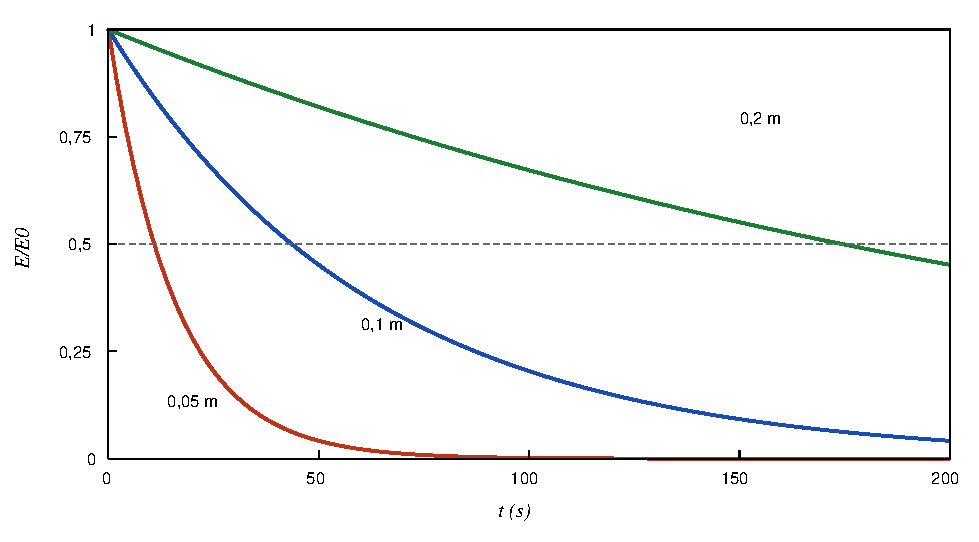
\includegraphics{../figures/FIG-0050/figure.pdf}}%
\count0=\ht0
\advance\count0 by \dp0
\count2=\wd0
\count4=\dimexpr\textheight/100*38\relax
\count6=\linewidth
\ifnum\count0<1
\count0=1
\fi
\ifnum\count2<1
\count2=1
\fi
\divide\count0 by 4096
\divide\count2 by 4096
\divide\count4 by 4096
\divide\count6 by 4096
\ifnum\count0<1
\count0=1
\fi
\ifnum\count2<1
\count2=1
\fi
\ifnum\count4<1
\count4=1
\fi
\ifnum\count6<1
\count6=1
\fi
\count8=\count2
\ifnum\count0>\count4
\count8=\numexpr\count2*\count4/\count0\relax
\fi
\ifnum\count8>\count6
\resizebox{\linewidth}{!}{\box0}%
\else
\ifnum\count0>\count4
\resizebox{!}{\dimexpr\textheight/100*38\relax}{\box0}%
\else
\box0%
\fi
\fi
\endgroup
\par\nopagebreak
\studiumcaption{fig:c14-decaimiento}{Fracción de la energía cinética inicial que conserva una red de torbellinos de Taylor-Green en agua (\(\nu = 1.007\times 10^{-6}\) m\(^2\)/s) para longitudes de onda de 0,05, 0.1 y 0.2 m; la línea discontinua marca la mitad de la energía inicial.}
\end{minipage}
\par\vspace{\baselineskip}

\par\vspace{\baselineskip}
\noindent\begin{minipage}{\linewidth}
\centering
\begingroup
\setbox0=\hbox{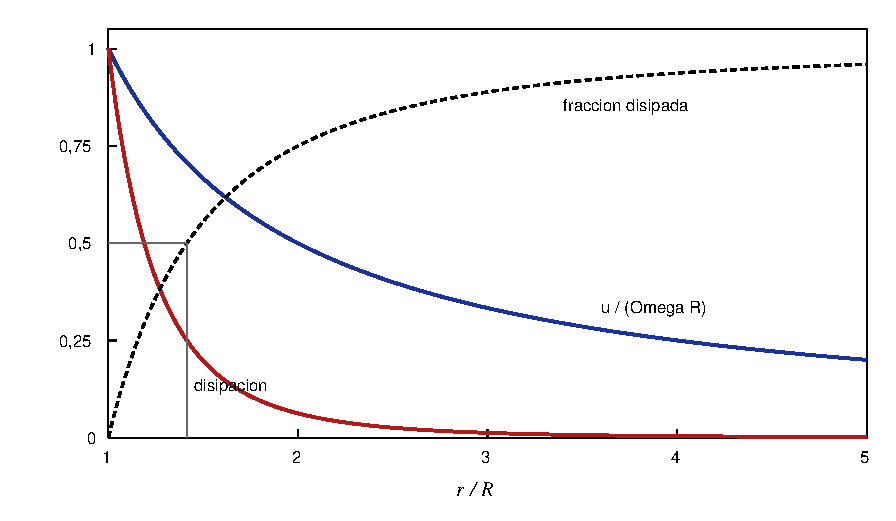
\includegraphics{../figures/FIG-0052/figure.pdf}}%
\count0=\ht0
\advance\count0 by \dp0
\count2=\wd0
\count4=\dimexpr\textheight/100*38\relax
\count6=\linewidth
\ifnum\count0<1
\count0=1
\fi
\ifnum\count2<1
\count2=1
\fi
\divide\count0 by 4096
\divide\count2 by 4096
\divide\count4 by 4096
\divide\count6 by 4096
\ifnum\count0<1
\count0=1
\fi
\ifnum\count2<1
\count2=1
\fi
\ifnum\count4<1
\count4=1
\fi
\ifnum\count6<1
\count6=1
\fi
\count8=\count2
\ifnum\count0>\count4
\count8=\numexpr\count2*\count4/\count0\relax
\fi
\ifnum\count8>\count6
\resizebox{\linewidth}{!}{\box0}%
\else
\ifnum\count0>\count4
\resizebox{!}{\dimexpr\textheight/100*38\relax}{\box0}%
\else
\box0%
\fi
\fi
\endgroup
\par\nopagebreak
\studiumcaption{fig:c14-disipacion}{Cilindro giratorio en un fluido ilimitado: velocidad \(u_\theta/(\Omega R) = R/r\) (azul), función de disipación \(\Phi/(4\mu\Omega^{2}) = (R/r)^{4}\) (rojo) y fracción acumulada de la potencia disipada dentro del radio \(r\), \(1 - R^{2}/r^{2}\) (negro discontinuo). La mitad de la potencia se disipa en \(r < \sqrt{2}\,R\).}
\end{minipage}
\par\vspace{\baselineskip}

\section{Fluidos ideales: ecuación de Euler}

En un fluido ideal, sin viscosidad, el tensor de esfuerzos es \(\boldsymbol{\sigma} = -p\,\mathbf{I}\), su divergencia es \(-\nabla p\) y la ecuación de Cauchy se convierte en la ecuación de Euler,
\begin{equation}
\rho\left(\frac{\partial\mathbf{u}}{\partial t} + (\mathbf{u}\cdot\nabla)\mathbf{u}\right) = -\nabla p + \rho\,\mathbf{g}. \label{eq:c14-euler}
\end{equation}
Proyectada sobre una línea de corriente en flujo estacionario, reproduce la ecuación \(\eqref{eq:c12-euler-s}\) del capítulo 12 y, con ella, la de Bernoulli. Usando la identidad cinemática \((\mathbf{u}\cdot\nabla)\mathbf{u} = \nabla(\tfrac12|\mathbf{u}|^{2}) - \mathbf{u}\times\boldsymbol{\omega}\), comprobada simbólicamente en este capítulo, la ecuación de Euler estacionaria e incompresible puede escribirse \(\nabla(p/\rho + \tfrac12|\mathbf{u}|^{2} + g z) = \mathbf{u}\times\boldsymbol{\omega}\). El segundo miembro es perpendicular a la velocidad, de modo que la cantidad entre paréntesis es constante a lo largo de cada línea de corriente; si además el flujo es irrotacional, el segundo miembro es nulo y la constante es la misma en todo el campo. Así queda demostrado el resultado que en el capítulo 12 se usó para el cilindro. Un ejemplo sencillo muestra cómo la presión acelera el fluido: en la tobera \(u = U_0(1 + x/L)\) del capítulo 4, la ecuación de Euler exige un gradiente de presión favorable \(dp/dx = -\rho U_0^{2}(1 + x/L)/L\), cuya integración devuelve la ecuación de Bernoulli. Tomando el rotacional de la ecuación de Euler se demuestra el teorema de Kelvin anunciado en el capítulo 12: en un fluido ideal, barótropo y con fuerzas de volumen conservativas, la circulación alrededor de una curva material no cambia.

\section{Ecuaciones de Navier-Stokes incompresibles}

Para un fluido newtoniano incompresible con viscosidad constante, el tensor de esfuerzos es \(\boldsymbol{\sigma} = -p\,\mathbf{I} + \mu(\nabla\mathbf{u} + \nabla\mathbf{u}^{\mathsf{T}})\). Su divergencia vale \(-\nabla p + \mu\nabla^{2}\mathbf{u} + \mu\nabla(\nabla\cdot\mathbf{u})\), y el último término es nulo por la continuidad. Sustituyendo en la ecuación de Cauchy se obtienen las ecuaciones de Navier-Stokes,
\begin{equation}
\rho\left(\frac{\partial\mathbf{u}}{\partial t} + (\mathbf{u}\cdot\nabla)\mathbf{u}\right) = -\nabla p + \mu\nabla^{2}\mathbf{u} + \rho\,\mathbf{g}, \qquad \nabla\cdot\mathbf{u} = 0, \label{eq:c14-ns}
\end{equation}
establecidas por Navier en 1822 y por Stokes entre 1842 y 1850, con contribuciones independientes de Poisson. Son cuatro ecuaciones para cuatro incógnitas, las tres componentes de la velocidad y la presión. Cada término tiene una interpretación física: el primer miembro es la masa por unidad de volumen por la aceleración, local y convectiva; en el segundo aparecen la fuerza neta de presión, la fuerza viscosa neta y el peso. El término viscoso \(\mu\nabla^{2}\mathbf{u}\) es un término de difusión de la cantidad de movimiento, con difusividad \(\nu\), análogo al de la ecuación del calor del capítulo 13. En flujo incompresible la presión no es una variable termodinámica determinada por una ecuación de estado, sino el campo que se ajusta en cada instante para que el campo de velocidades sea solenoidal. En coordenadas cartesianas, la componente \(x\) es
\begin{equation}
\rho\left(\frac{\partial u}{\partial t} + u\frac{\partial u}{\partial x} + v\frac{\partial u}{\partial y} + w\frac{\partial u}{\partial z}\right) = -\frac{\partial p}{\partial x} + \mu\left(\frac{\partial^{2}u}{\partial x^{2}} + \frac{\partial^{2}u}{\partial y^{2}} + \frac{\partial^{2}u}{\partial z^{2}}\right) + \rho g_x. \label{eq:c14-ns-x}
\end{equation}
Las condiciones de contorno son las del capítulo 4: no deslizamiento en las paredes, condiciones de entrada y salida o de corriente libre, y condiciones iniciales en problemas no estacionarios.

El término convectivo hace las ecuaciones no lineales, y no se conoce ninguna solución general; si para cualquier dato inicial suave existen soluciones suaves en tres dimensiones es, de hecho, uno de los problemas matemáticos abiertos más famosos, uno de los siete Problemas del Milenio. Las pocas soluciones exactas conocidas corresponden a geometrías en las que el término convectivo se anula o se simplifica. Los flujos de Couette y Poiseuille del capítulo 6 son soluciones exactas: el flujo es unidireccional y completamente desarrollado, la aceleración convectiva es nula y la ecuación \(\eqref{eq:c14-ns-x}\) se reduce a \(0 = -dp/dx + \mu\,d^{2}u/dy^{2}\), exactamente la ecuación que allí se obtuvo con un balance de fuerzas. Un ejemplo no estacionario y bidimensional es el torbellino de Taylor-Green,
\begin{equation}
u = \sin x\cos y\,e^{-2\nu t},\qquad v = -\cos x\sin y\,e^{-2\nu t},\qquad p = \tfrac{\rho}{4}(\cos 2x + \cos 2y)\,e^{-4\nu t}, \label{eq:c14-tg}
\end{equation}
en variables adimensionales con número de onda unidad: una red de torbellinos alternados, representada en la figura~\ref{fig:c14-taylor-green}, que decae por la viscosidad sin cambiar de forma; con número de onda dimensional \(k_w\), la energía cinética decae como \(e^{-4\nu k_w^{2} t}\), tanto más deprisa cuanto menor es la escala, como muestra la figura~\ref{fig:c14-decaimiento} para el agua. Sustituyendo en las ecuaciones se comprueba que el término convectivo, \(\tfrac12\sin 2x\,e^{-4\nu t}\), se equilibra exactamente con el gradiente de presión, y que la derivada temporal se equilibra con el término viscoso; esa comprobación se ha hecho simbólicamente para este libro. La solución se usa a menudo para validar programas de cálculo. Fuera de estos casos, las ecuaciones de Navier-Stokes se resuelven numéricamente, con métodos de diferencias, volúmenes o elementos finitos, o se simplifican con aproximaciones justificadas por el análisis de órdenes de magnitud, como las del capítulo 15. Con ellas se diseñan aviones y motores, se estudian el flujo sanguíneo y la contaminación atmosférica, y se predice el tiempo.

\section{Momento angular y energía}

El principio de conservación del momento angular, aplicado a un volumen material igual que el del momento lineal, no da una ecuación nueva para un fluido sin pares internos: su único contenido local es la simetría del tensor de esfuerzos demostrada en el capítulo 13, que ya se ha usado al construir la ley constitutiva. Su forma integral es, sin embargo, muy útil en las turbomáquinas: aplicada a un volumen de control que encierra el rotor de un compresor o de una turbina, da el par en función del cambio del momento angular del fluido entre la entrada y la salida, que es la ecuación de Euler de las turbomáquinas. La conservación de la energía conduce a la ecuación de la energía total, que añade a la energía cinética la energía interna, el trabajo de las fuerzas de superficie y el calor conducido según la ley de Fourier; en flujos incompresibles sin efectos térmicos importantes, la energía interna se desacopla y basta con la ecuación de la energía mecánica, que se obtiene multiplicando escalarmente las ecuaciones de Navier-Stokes por la velocidad.

El resultado de esa multiplicación es una ecuación de balance para la energía cinética por unidad de volumen, \(\tfrac12\rho|\mathbf{u}|^{2}\): su variación siguiendo al fluido se debe al trabajo de la presión, al del peso, al transporte de energía por los esfuerzos viscosos y a un término siempre negativo,
\begin{equation}
-\Phi_v, \qquad \Phi_v = 2\mu\,\mathbf{E}:\mathbf{E} = 2\mu\,E_{ij}E_{ij} \ge 0, \label{eq:c14-disipacion}
\end{equation}
la función de disipación, que mide la potencia por unidad de volumen que la viscosidad convierte irreversiblemente en energía interna. Que sea siempre positiva refleja el segundo principio de la termodinámica, y es la razón por la que la viscosidad debe ser positiva. En el flujo de Couette, \(\Phi_v = \mu(du/dy)^{2} = \mu(U/h)^{2}\) es uniforme; integrada en la holgura da \(\mu U^{2}/h\), exactamente la potencia por unidad de área que aporta la placa móvil, \(\tau_w U\). Toda la energía que suministra el motor se transforma en calor, como se intuía en el cojinete del capítulo 3. En flujos turbulentos la disipación se concentra en los torbellinos más pequeños, a los que la energía llega desde los grandes a través de una cascada; es la razón última de la mayor resistencia de esos flujos.

\section{Fuerza neta por unidad de volumen, gradiente de presión y término viscoso}

Muchos problemas de examen piden la fuerza neta que actúa sobre un elemento de fluido, por unidad de volumen, en un punto de un campo de velocidad conocido. La clave es que la segunda ley de Newton aplicada a una partícula fluida de masa \(\rho\,dV\) dice que la fuerza neta sobre ella es su masa por su aceleración, y que la aceleración de la partícula es la derivada material de la velocidad. Por unidad de volumen,
\begin{equation}
\mathbf{f} = \rho\,\frac{D\mathbf{u}}{Dt} = -\nabla p + \mu\nabla^{2}\mathbf{u}, \label{eq:c14-fuerza-neta}
\end{equation}
donde la segunda igualdad identifica de qué fuerzas se compone la fuerza neta en un fluido newtoniano incompresible sin gravedad. El orden lógico importa: la fuerza neta se obtiene solo con la cinemática, derivando el campo de velocidad, sin conocer la presión; las ecuaciones de Navier--Stokes permiten después identificar presión, viscosidad y fuerzas de volumen \emph{solo si el campo prescrito es dinámicamente compatible con esas hipótesis}. Sin fuerzas de volumen, el candidato a gradiente es \(\nabla p = -\rho\,D\mathbf{u}/Dt + \mu\nabla^{2}\mathbf{u}\), y debe ser irrotacional para corresponder a una presión escalar.

El término viscoso admite una forma muy útil. Para un campo con divergencia nula, la identidad vectorial del laplaciano da \(\nabla^{2}\mathbf{u} = -\nabla\times\boldsymbol{\omega}\): la fuerza viscosa neta sobre un elemento solo existe donde la vorticidad varía en el espacio. En particular, en un flujo incompresible e irrotacional el término viscoso de \(\eqref{eq:c14-fuerza-neta}\) es idénticamente nulo aunque el fluido sea viscoso, y la fuerza neta la proporciona entera el gradiente de presión. Para el campo del ejemplo resuelto del capítulo 12, \(\psi = K\,(x^{2}y + 2xy^{2})\), la vorticidad es \(\omega_z = -K\,(4x + 2y)\) y el laplaciano de la velocidad vale \((2K, -4K)\), constante. Con agua (viscosidad de \(10^{-3}\) Pa s) y \(K\) de 1 m\(^{-1}\)s\(^{-1}\), la fuerza viscosa por unidad de volumen tiene componentes \((0.002;\ -0.004)\) N/m\(^3\), frente a una fuerza inercial requerida de casi \(10^{5}\) N/m\(^3\) en el punto \((1,2)\). Pero esa comparación \emph{no autoriza} a concluir que la presión equilibra la inercia: el rotacional del candidato a gradiente de presión cumple \[\begin{aligned}\partial_x(\mu\nabla^{2}v-\rho a_y)-\partial_y(\mu\nabla^{2}u-\rho a_x)\\ &=4\rho K^{2}(x^{2}+3xy-y^{2})\end{aligned}\], que no se anula en general (vale \(12\,000\) N/m\(^4\) en el punto). Ninguna presión escalar puede producir ese gradiente en un entorno del punto bajo las hipótesis adoptadas. El campo es válido como ejercicio cinemático, pero exige fuerzas de volumen adicionales no conservativas para ser una solución dinámica estacionaria. En un aceite muy viscoso que se mueve despacio la proporción se invierte, como muestra el último ejercicio del capítulo.

\section{Flujos azimutales entre y alrededor de cilindros giratorios}

El capítulo 6 obtuvo el flujo de Couette circular con un equilibrio de pares sobre una capa cilíndrica. Las ecuaciones de Navier-Stokes en coordenadas cilíndricas \((r, \theta, z)\) permiten deducirlo de forma general y obtener, además, la presión y la disipación. Busquemos una solución estacionaria con velocidad puramente azimutal, \(\mathbf{u} = u_\theta(r)\,\mathbf{e}_\theta\). La continuidad se cumple automáticamente, porque \(u_\theta\) no depende de \(\theta\). La componente radial de las ecuaciones contiene la aceleración centrípeta, que no es nula aunque el flujo sea estacionario: cada partícula describe una circunferencia y necesita una fuerza dirigida hacia el eje, que solo puede proporcionar la presión,
\begin{equation}
\frac{dp}{dr} = \frac{\rho\,u_\theta^{2}}{r}. \label{eq:c14-radial}
\end{equation}
La componente azimutal no tiene aceleración ni gradiente de presión (la presión no puede depender de \(\theta\) en un dominio que da la vuelta completa al eje), de modo que el término viscoso debe anularse por sí solo:
\begin{equation}
\mu\left(\frac{d^{2}u_\theta}{dr^{2}} + \frac{1}{r}\frac{du_\theta}{dr} - \frac{u_\theta}{r^{2}}\right) = 0. \label{eq:c14-azimutal}
\end{equation}
El término \(-u_\theta/r^{2}\) no aparece en coordenadas cartesianas: procede de que los vectores de la base cilíndrica cambian de dirección al moverse alrededor del eje, y olvidarlo es el error más frecuente al simplificar estas ecuaciones.

El operador de \(\eqref{eq:c14-azimutal}\) es una derivada exacta, \(\frac{d}{dr}\!\left[\frac{1}{r}\,\frac{d}{dr}\left(r\,u_\theta\right)\right] = 0\), de modo que dos integraciones dan \(u_\theta = A\,r + B/r\), la misma solución del capítulo 6. Las constantes se fijan con las condiciones de contorno. Entre dos cilindros, con el no deslizamiento en ambas paredes, se recupera el flujo de Couette circular. Para un único cilindro de radio \(R\) que gira con velocidad angular \(\Omega\) en un fluido ilimitado en reposo en el infinito, la velocidad no puede crecer indefinidamente con \(r\), lo que exige \(A = 0\), y el no deslizamiento en \(r = R\) da \(B = \Omega R^{2}\). El resultado es un torbellino libre, \(u_\theta = \Omega R^{2}/r\), cuya vorticidad \(\omega_z = \frac{1}{r}\frac{d}{dr}(r\,u_\theta)\) es nula en todo el fluido. Es un ejemplo notable: el flujo es irrotacional, el término viscoso de las ecuaciones se anula, como anticipaba la identidad \(\nabla^{2}\mathbf{u} = -\nabla\times\boldsymbol{\omega}\), y sin embargo los esfuerzos viscosos no son nulos, porque las capas de fluido giran con velocidades angulares distintas y se deforman. La viscosidad no ejerce fuerza neta sobre cada elemento, pero sí transmite par, y la pared necesita un motor para mantener el giro.

El esfuerzo cortante en la pared es \(\tau_{r\theta}(R) = -2\mu\Omega\), y el par que el motor aplica por unidad de longitud es \(T' = 2\pi R^{2}\cdot 2\mu\Omega = 4\pi\mu\Omega R^{2}\), con una potencia \(T'\,\Omega = 4\pi\mu\Omega^{2}R^{2}\). Hay una comprobación independiente de este resultado: en régimen estacionario la energía cinética del fluido no cambia, de modo que toda la potencia del motor debe disiparse en calor dentro del fluido. La potencia disipada por unidad de volumen en un flujo de cizalla azimutal es
\begin{equation}
\Phi = \mu\left[r\,\frac{d}{dr}\!\left(\frac{u_\theta}{r}\right)\right]^{2} = \frac{4\mu\Omega^{2}R^{4}}{r^{4}}, \label{eq:c14-phi}
\end{equation}
siempre positiva, y la presión no contribuye a ella. Integrando sobre una corona entre \(R\) y \(R_2\) se obtiene \(4\pi\mu\Omega^{2}R^{2}\left(1 - R^{2}/R_2^{2}\right)\), que tiende a \(4\pi\mu\Omega^{2}R^{2}\) cuando \(R_2 \to \infty\): coincide con la potencia del motor, como debía. La expresión enseña además dónde se disipa la energía: la mitad dentro de \(r < \sqrt{2}\,R\) y el 90 \% dentro de \(r < \sqrt{10}\,R\), como muestra la figura~\ref{fig:c14-disipacion}. La presión, por \(\eqref{eq:c14-radial}\), vale \(p(r) = p_\infty - \rho\,\Omega^{2}R^{4}/(2r^{2})\): es mínima junto al cilindro, como en el núcleo de un remolino.

Ejemplo resuelto. Un eje de 10 mm de radio gira a 300 rad/s en un gran baño de glicerina, de viscosidad 1.41 Pa s y densidad 1260 kg/m\(^3\). Sistema y ejes: coordenadas cilíndricas con el eje \(z\) a lo largo del eje; incógnitas, el par y la potencia por unidad de longitud. Hipótesis: régimen estacionario y laminar, fluido ilimitado en reposo lejos del eje, sin efectos de extremo ni gravedad. Antes de calcular conviene comprobar el régimen con el número de Reynolds de rotación, \(\Omega R^{2}\rho/\mu\): \(300\cdot 0.010^2\cdot 1260/1.41 = 26.81\), bajo, compatible con un flujo laminar. El par por unidad de longitud es \(4\pi\cdot 1.41\cdot 300\cdot 0.010^2 = 0.53156\) N m/m y la potencia, \(4\pi\cdot 1.41\cdot 300^2\cdot 0.010^2 = 159.47\) W/m. Comprobación dimensional: Pa s por s\(^{-2}\) por m\(^2\) da W/m. La mitad de esa potencia se disipa a menos de \(\sqrt{2}\cdot 10 = 14.14\) mm del eje, y la presión en la pared es \(1260\cdot 300^2\cdot 0.010^2/2 = 5670\) Pa inferior a la del baño lejano. Interpretación: el resultado depende de la viscosidad y del cuadrado de la velocidad angular; si el baño tuviera una pared a pocos milímetros, la potencia aumentaría según el factor \(R_2^{2}/(R_2^{2} - R^{2})\) del capítulo 6.

El régimen estacionario de un cilindro en un fluido ilimitado es una idealización que merece una advertencia. La rotación se transmite al fluido por difusión viscosa, y la distancia a la que ha llegado tras un tiempo \(t\) es del orden de \(\sqrt{\nu t}\); por tanto el perfil \(\tfrac{1}{r}\) solo está establecido hasta esa distancia, y en un depósito real la pared exterior acaba imponiendo el flujo de Couette circular. Además, la solución laminar deja de observarse cuando el número de Reynolds de rotación es alto: entre cilindros, el giro del cilindro interior produce los torbellinos de Taylor por encima de un número de Taylor crítico. Por último, los cilindros reales son finitos y los extremos generan flujos secundarios. Estas limitaciones no restan valor al modelo, que da el orden de magnitud correcto del par y es exacto en las condiciones supuestas, pero obligan a comprobarlas antes de aplicarlo.

\begin{tcolorbox}[title={Consejo}, studiumtip, breakable]

Ante un problema nuevo, no intente resolver las ecuaciones de Navier-Stokes completas. Escriba sus componentes, elimine con argumentos físicos los términos nulos (por simetría, estacionariedad o flujo desarrollado) y estime el orden de magnitud de los restantes antes de despreciar ninguno; las soluciones exactas y aproximadas de este libro se obtienen así.

Al simplificar las ecuaciones de Navier-Stokes en coordenadas cilíndricas, escriba primero qué componentes de la velocidad existen y de qué variables dependen, y después elimine términos uno a uno justificando cada eliminación. Recuerde que un flujo estacionario no tiene por qué tener aceleración nula: en un flujo circular la aceleración centrípeta \(u_\theta^{2}/r\) existe siempre y la equilibra el gradiente radial de presión. Compruebe el resultado final con un balance de energía: la potencia del motor debe coincidir con la integral de la disipación.
\end{tcolorbox}

\begin{tcolorbox}[title={Definición}, studiumdef, breakable]

Ecuaciones de Navier-Stokes: ecuaciones de conservación de la cantidad de movimiento de un fluido newtoniano viscoso, obtenidas al sustituir la ley constitutiva newtoniana en la ecuación de Cauchy. Junto con la ecuación de continuidad, y en general la de la energía, gobiernan el movimiento de líquidos y gases en el modelo de medio continuo.
\end{tcolorbox}



% Revision bibliografica 2026: material original, contrastes verificables.

\section{Contraste bibliográfico: esfuerzo viscoso no equivale a fuerza viscosa}
\label{sec:ref26-ns}

La conservación de la masa de un medio continuo se expresa como \(\partial_t\rho+\nabla\cdot(\rho\mathbf{u})=0\). La condición \(\nabla\cdot\mathbf{u}=0\) se deduce cuando la densidad de cada partícula permanece constante, es decir, \(D\rho/Dt=0\) y \(\rho>0\); no debe introducirse sin justificarla para un gas compresible. Para densidad y viscosidad constantes y fluido newtoniano incompresible, sin otras fuerzas volumétricas,
\begin{equation}
 \nabla\cdot\mathbf{u}=0,\qquad
 \rho\,\frac{D\mathbf{u}}{Dt}=-\nabla p+\mu\nabla^2\mathbf{u}.
 \label{eq:ref26-ns-form}
\end{equation}
El término \(\mu\nabla^2\mathbf{u}\) es la \emph{divergencia del tensor viscoso}, no el tensor de esfuerzos viscosos \(\boldsymbol{\tau}=2\mu\mathbf{E}\) en sí. Una distribución de esfuerzos puede ser distinta de cero y poseer divergencia nula. Para viscosidad espacialmente variable se debe conservar \(\nabla\cdot(2\mu\mathbf{E})\), y no reemplazarlo sin más por \(\mu\nabla^2\mathbf{u}\).

\begin{tcolorbox}[title={Ejemplo guiado original: deformación plana}, studiumdef, breakable]
Considérese, lejos de fronteras sólidas, el campo bidimensional estacionario \(\mathbf{u}=(ax,-ay,0)\), con \(a\) constante. Su divergencia es \(a-a=0\), la aceleración material es \((a^2x,a^2y,0)\), y \(\nabla^2\mathbf{u}=\mathbf{0}\). La presión
\[
 p(x,y)=p_0-\frac{\rho a^2}{2}(x^2+y^2)
\]
satisface exactamente la ecuación de cantidad de movimiento. Pero
\[
 \mathbf{E}=\operatorname{diag}(a,-a,0),
 \qquad\boldsymbol{\tau}=2\mu\operatorname{diag}(a,-a,0)\ne\mathbf{0}.
\]
Por ejemplo, si \(a=2\,\mathrm{s^{-1}}\), \(\rho=1000\,\mathrm{kg\,m^{-3}}\) y \(\mu=0.001\,\mathrm{Pa\,s}\), los esfuerzos normales viscosos son \(+0.004\) y \(-0.004\,\mathrm{Pa}\), y en \((x,y)=(0.20,0.10)\,\mathrm{m}\) la presión es \(100\,\mathrm{Pa}\) menor que \(p_0\). Esto es una solución local idealizada, no una predicción sobre cómo se mantiene el campo en un recipiente finito.
\end{tcolorbox}

\textbf{Autocomprobación.} Calcule el rotacional del campo y distinga «flujo irrotacional» de «sin deformación viscosa». Discuta qué término reaparecería si \(\mu=\mu(x,y)\). Ejemplo y verificación algebraica propios, contrastados con los capítulos 4 de White \cite{ref26-white} y 11 de Shaughnessy, Katz y Schaffer \cite{ref26-shaughnessy}. Para la notación de gradiente y divergencia, véase Boas, capítulo 6 \cite{ref26-boas}.


\section{Desarrollos y práctica}

Las deducciones de este capítulo obtienen las ecuaciones del movimiento de un fluido a partir de la ecuación de Cauchy \(\eqref{eq:c14-cauchy}\): la de Euler \(\eqref{eq:c14-euler}\) para un fluido ideal, la forma de Lamb de la aceleración convectiva y las ecuaciones de Navier-Stokes incompresibles \(\eqref{eq:c14-ns}\), cuya componente cartesiana \(\eqref{eq:c14-ns-x}\) se usa en los ejercicios. La solución de Taylor-Green \(\eqref{eq:c14-tg}\) y el balance de disipación viscosa \(\eqref{eq:c14-disipacion}\) permiten comprobar sobre casos concretos que las ecuaciones son coherentes. En los problemas conviene verificar primero que el campo propuesto cumple la continuidad y después sustituirlo en cada componente de la ecuación de cantidad de movimiento.

\begin{tcolorbox}[title={Desarrollos del modelo}, studiumdef, breakable]

\noindent\textbf{Euler unidimensional en una tobera y presión que acelera el fluido}

\begin{equation}
\rho u\frac{du}{dx} = -\frac{dp}{dx}:\qquad u = U_0\left(1 + \frac{x}{L}\right)\ \Rightarrow\ p = p_0 - \tfrac12\rho U_0^{2}\left[\left(1 + \frac{x}{L}\right)^{2} - 1\right]
\label{eq:c14-euler-1d}
\end{equation}

\noindent\textbf{Hipótesis}
\begin{itemize}
\item flujo estacionario, unidimensional, incompresible y no viscoso
\item campo de velocidad de la tobera del capítulo 4
\end{itemize}

\noindent\textbf{Limitaciones}
\begin{itemize}
\item la aceleración convectiva exige un gradiente de presión favorable
\end{itemize}

\noindent\textbf{Pasos}
\begin{enumerate}
\item
proyectar la ecuación de Euler sobre el eje

\[
\frac{dp}{dx} = -\rho\,U_0^{2}\left(1 + \frac{x}{L}\right)\frac{1}{L}
\]
\item
sustituir el campo de velocidad

\[
p + \tfrac12\rho u^{2} = p_0 + \tfrac12\rho U_0^{2}
\]
\item
integrar: se recupera Bernoulli

\[
dp/dx = -\rho U_0^{2}(1 + x/L)/L
\]
\item
relación usada en el texto (paso intermedio no comprobado por separado)
\end{enumerate}

\noindent\textbf{Variables}
\begin{itemize}
\item $U_{0}$: velocidad en la entrada ($\mathrm{m}\,\mathrm{s}^{-1}$)
\end{itemize}



\noindent\textbf{Forma de Lamb de la aceleración convectiva}

\begin{equation}
(\mathbf{u}\cdot\nabla)\mathbf{u} = \nabla\!\left(\tfrac12|\mathbf{u}|^{2}\right) - \mathbf{u}\times\boldsymbol{\omega}
\label{eq:c14-lamb}
\end{equation}

\noindent\textbf{Hipótesis}
\begin{itemize}
\item campo de velocidad derivable
\end{itemize}

\noindent\textbf{Limitaciones}
\begin{itemize}
\item identidad cinemática: válida para cualquier flujo
\end{itemize}

\noindent\textbf{Pasos}
\begin{enumerate}
\item
escribir la componente x en un flujo plano

\[
u\,u_x + v\,u_y = \left(u\,u_x + v\,v_x\right) - v\,(v_x - u_y)
\]
\item
sustituir omega\(_z = dv/dx - du/dy\)
\item
comparar ambos miembros
\end{enumerate}

\noindent\textbf{Variables}
\begin{itemize}
\item $\omega$: vorticidad ($\mathrm{1/s}$)
\end{itemize}



\noindent\textbf{Ecuaciones de Navier-Stokes incompresibles}

\[
\rho\left(\frac{\partial\mathbf{u}}{\partial t} + (\mathbf{u}\cdot\nabla)\mathbf{u}\right) = -\nabla p + \mu\nabla^{2}\mathbf{u} + \rho\mathbf{g},\qquad \nabla\cdot\mathbf{u} = 0
\]

\noindent\textbf{Hipótesis}
\begin{itemize}
\item fluido newtoniano
\item densidad y viscosidad constantes
\item flujo incompresible
\end{itemize}

\noindent\textbf{Limitaciones}
\begin{itemize}
\item con viscosidad variable o compresibilidad aparecen términos adicionales
\end{itemize}

\noindent\textbf{Pasos}
\begin{enumerate}
\item
sustituir sigma = -p I + mu (grad u + grad \(u^T)\) en la ecuación de Cauchy

\[
\nabla\cdot\boldsymbol{\tau} = \mu\nabla^{2}\mathbf{u} + \mu\nabla(\nabla\cdot\mathbf{u}) = \mu\nabla^{2}\mathbf{u}
\]
\item
usar div(grad \(u^T) =\) grad(div u) = 0

\[
u = \sin x\cos y\,e^{-2\nu t},\quad v = -\cos x\sin y\,e^{-2\nu t},\quad p = \tfrac{\rho}{4}(\cos 2x + \cos 2y)\,e^{-4\nu t}
\]
\item
comprobación con una solución exacta: el torbellino de Taylor-Green

\[
\boldsymbol{\sigma} = -p\,\mathbf{I} + \mu(\nabla\mathbf{u} + \nabla\mathbf{u}^{\mathsf{T}})
\]
\item
relación usada en el texto (paso intermedio no comprobado por separado)

\[
0 = -dp/dx + \mu\,d^{2}u/dy^{2}
\]
\item
relación usada en el texto (paso intermedio no comprobado por separado)
\end{enumerate}

\noindent\textbf{Variables}
\begin{itemize}
\item $\nu$: viscosidad cinemática ($\mathrm{m}^{2}\,\mathrm{s}^{-1}$)
\end{itemize}



\noindent\textbf{La disipación viscosa en el flujo de Couette iguala la potencia aportada}

\[
\int_0^{h}\Phi_v\,dy = \int_0^{h}\mu\left(\frac{du}{dy}\right)^{2}dy = \mu\frac{U^{2}}{h} = \tau_w U
\]

\noindent\textbf{Hipótesis}
\begin{itemize}
\item flujo de Couette sin gradiente de presión
\item régimen estacionario
\end{itemize}

\noindent\textbf{Limitaciones}
\begin{itemize}
\item toda la potencia aportada se convierte en calor; en régimen estacionario ese calor debe evacuarse
\end{itemize}

\noindent\textbf{Pasos}
\begin{enumerate}
\item
la función de disipación en flujo cortante simple es mu \((du/dy)^2\)

\[
\Phi_v = 2\mu\,\mathbf{E}:\mathbf{E} = \mu\left(\frac{du}{dy}\right)^{2}
\]
\item
integrar sobre la holgura
\item
comparar con la potencia que la placa aporta, tau\(_w U\)
\end{enumerate}

\noindent\textbf{Variables}
\begin{itemize}
\item $U$: velocidad de la placa ($\mathrm{m}\,\mathrm{s}^{-1}$)
\end{itemize}



\noindent\textbf{Gradiente de presión a partir de la aceleración y del término viscoso}

\begin{equation}
\mathbf{f} = \rho\,\frac{D\mathbf{u}}{Dt} = -\nabla p + \mu\nabla^{2}\mathbf{u},\qquad \nabla^{2}\mathbf{u} = -\nabla\times\boldsymbol{\omega}
\label{eq:c14-fuerza-presion}
\end{equation}

\noindent\textbf{Hipótesis}
\begin{itemize}
\item fluido newtoniano e incompresible
\item sin fuerzas de volumen (o incluidas en una presión modificada)
\end{itemize}

\noindent\textbf{Principios}
\begin{itemize}
\item segunda ley de Newton por unidad de volumen
\item identidad vectorial del laplaciano para campos solenoidales
\end{itemize}

\noindent\textbf{Aplicabilidad}
\begin{itemize}
\item separar la fuerza neta, conocida a partir del campo de velocidad, de las fuerzas de presión y viscosas
\end{itemize}

\noindent\textbf{Limitaciones}
\begin{itemize}
\item la presión solo se obtiene si el campo de velocidad es compatible con las ecuaciones (rotacional de la ecuación nulo)
\end{itemize}

\noindent\textbf{Pasos}
\begin{enumerate}
\item
fuerza neta por unidad de volumen = densidad por aceleración material

\[
\mathbf{f} = \rho\,\frac{D\mathbf{u}}{Dt}
\]
\item
Navier-Stokes incompresible sin gravedad

\[
\nabla p = -\rho\,\frac{D\mathbf{u}}{Dt} + \mu\nabla^{2}\mathbf{u}
\]
\item
en un campo con divergencia nula el laplaciano es menos el rotacional de la vorticidad

\[
\nabla^{2}\mathbf{u} = \nabla(\nabla\cdot\mathbf{u}) - \nabla\times(\nabla\times\mathbf{u}) = -\nabla\times\boldsymbol{\omega}
\]
\item
ejemplo psi \(= K(x^2 y + 2 x y^2)\): laplaciano (2, -4) K = -rotacional de omega

\[
\omega_z = -K\,(4x + 2y),\qquad \nabla^{2}\mathbf{u} = (2K, -4K)
\]
\end{enumerate}

\noindent\textbf{Variables}
\begin{itemize}
\item $\mathbf{f}$: fuerza neta por unidad de volumen ($\mathrm{N}\,\mathrm{m}^{-3}$)
\item $\boldsymbol{\omega}$: vorticidad ($\mathrm{1/s}$)
\end{itemize}



\noindent\textbf{Navier-Stokes azimutal en coordenadas cilíndricas}

\begin{equation}
\frac{d}{dr}\!\left[\frac{1}{r}\,\frac{d}{dr}\left(r\,u_\theta\right)\right] = 0 \;\Rightarrow\; u_\theta = A\,r + \frac{B}{r},\qquad \frac{dp}{dr} = \frac{\rho\,u_\theta^{2}}{r}
\label{eq:c14-ns-azimutal}
\end{equation}

\noindent\textbf{Hipótesis}
\begin{itemize}
\item flujo estacionario, laminar e incompresible
\item \(u = u_theta(r) e_theta\), sin componentes radial ni axial
\item sin gravedad y sin gradiente de presión azimutal
\item cilindros infinitamente largos
\end{itemize}

\noindent\textbf{Principios}
\begin{itemize}
\item ecuaciones de Navier-Stokes en coordenadas cilíndricas
\end{itemize}

\noindent\textbf{Condiciones de contorno}
\begin{itemize}
\item no deslizamiento en cada cilindro
\item velocidad nula en el infinito para un fluido ilimitado (A = 0)
\end{itemize}

\noindent\textbf{Aplicabilidad}
\begin{itemize}
\item flujo de Couette circular
\item cilindro giratorio en un fluido ilimitado
\end{itemize}

\noindent\textbf{Limitaciones}
\begin{itemize}
\item solución laminar; inestable a número de Taylor alto
\item sin efectos de extremo
\end{itemize}

\noindent\textbf{Pasos}
\begin{enumerate}
\item
continuidad: la divergencia de \(u_theta(r) e_theta\) es nula

\[
\nabla\cdot\mathbf{u} = \frac{1}{r}\frac{\partial u_\theta}{\partial\theta} = 0
\]
\item
componente r: la aceleración centrípeta la produce el gradiente radial de presión

\[
-\rho\,\frac{u_\theta^{2}}{r} = -\frac{dp}{dr}
\]
\item
componente theta: el término viscoso debe anularse

\[
\mu\left(\frac{d^{2}u_\theta}{dr^{2}} + \frac{1}{r}\frac{du_\theta}{dr} - \frac{u_\theta}{r^{2}}\right) = 0
\]
\item
el operador se escribe como una derivada exacta

\[
\frac{d}{dr}\!\left[\frac{1}{r}\,\frac{d}{dr}\left(r\,u_\theta\right)\right] = 0
\]
\item
integrar dos veces

\[
u_\theta = A\,r + \frac{B}{r}
\]
\end{enumerate}

\noindent\textbf{Variables}
\begin{itemize}
\item $A$: constante de rotación rígida ($\mathrm{1/s}$)
\item $B$: constante de torbellino libre ($\mathrm{m}^{2}\,\mathrm{s}^{-1}$)
\end{itemize}



\noindent\textbf{Presión alrededor de un cilindro giratorio en un fluido ilimitado}

\begin{equation}
p(r) = p_\infty - \frac{\rho\,\Omega^{2}R^{4}}{2\,r^{2}}
\label{eq:c14-presion-vortice}
\end{equation}

\noindent\textbf{Hipótesis}
\begin{itemize}
\item torbellino libre \(u_theta =\) Omega \(R^2/r\)
\item sin gravedad
\end{itemize}

\noindent\textbf{Principios}
\begin{itemize}
\item componente radial de Navier-Stokes
\end{itemize}

\noindent\textbf{Limitaciones}
\begin{itemize}
\item la presión en un fluido real con superficie libre incluiría además la hidrostática
\end{itemize}

\noindent\textbf{Pasos}
\begin{enumerate}
\item
sustituir el torbellino libre en dp/dr = rho \(u^2/r\)

\[
\frac{dp}{dr} = \frac{\rho\,\Omega^{2}R^{4}}{r^{3}}
\]
\item
integrar desde r hasta el infinito

\[
p(r) = p_\infty - \frac{\rho\,\Omega^{2}R^{4}}{2\,r^{2}}
\]
\end{enumerate}

\noindent\textbf{Variables}
\begin{itemize}
\item $p_\infty$: presión lejos del cilindro ($\mathrm{Pa}$)
\end{itemize}



\noindent\textbf{La disipación viscosa alrededor de un cilindro giratorio iguala la potencia del motor}

\begin{equation}
\Phi = \mu\left[r\,\frac{d}{dr}\!\left(\frac{u_\theta}{r}\right)\right]^{2} = \frac{4\mu\Omega^{2}R^{4}}{r^{4}},\qquad \int_R^{\infty}\Phi\,2\pi r\,dr = 4\pi\mu\Omega^{2}R^{2} = T'\,\Omega
\label{eq:c14-disipacion-cilindro}
\end{equation}

\noindent\textbf{Hipótesis}
\begin{itemize}
\item torbellino libre \(u_theta =\) Omega \(R^2/r\)
\item flujo estacionario
\end{itemize}

\noindent\textbf{Principios}
\begin{itemize}
\item ecuación de la energía mecánica: en régimen estacionario la potencia aportada se disipa
\end{itemize}

\noindent\textbf{Aplicabilidad}
\begin{itemize}
\item comprobación energética independiente del cálculo del par
\end{itemize}

\noindent\textbf{Limitaciones}
\begin{itemize}
\item la mitad de la potencia se disipa en r < sqrt(2) R: el resultado es sensible a la capa próxima a la pared
\end{itemize}

\noindent\textbf{Pasos}
\begin{enumerate}
\item
función de disipación para un flujo de cizalla azimutal

\[
\Phi = \frac{\tau_{r\theta}^{2}}{\mu} = \frac{4\mu\Omega^{2}R^{4}}{r^{4}}
\]
\item
esfuerzo en la pared y par del motor

\[
\tau_{r\theta}(R) = -2\mu\Omega,\qquad T' = 2\pi R^{2}\cdot 2\mu\Omega = 4\pi\mu\Omega R^{2}
\]
\item
potencia disipada en la corona entre R y R2

\[
\int_R^{R_2}\Phi\,2\pi r\,dr = 4\pi\mu\Omega^{2}R^{2}\left(1 - \frac{R^{2}}{R_2^{2}}\right)
\]
\item
límite R2 -> infinito

\[
\int_R^{\infty}\Phi\,2\pi r\,dr = 4\pi\mu\Omega^{2}R^{2}
\]
\end{enumerate}

\noindent\textbf{Variables}
\begin{itemize}
\item $\Phi$: potencia disipada por unidad de volumen ($\mathrm{W}\,\mathrm{m}^{-3}$)
\end{itemize}


\end{tcolorbox}

\begin{tcolorbox}[title={Problema resuelto}, studiumworked, breakable]

\noindent\textbf{Enunciado}
En un tanque de agua (\(\nu = 1.007\times 10^{-6}\) m\(^2\)/s) se genera una red de torbellinos de Taylor-Green con longitud de onda \(\lambda_w = 0.10\) m, es decir, con número de onda \(k_w = 2\pi/\lambda_w\). En variables dimensionales la velocidad decae como \(e^{-2\nu k_w^{2} t}\) y la energía cinética como \(e^{-4\nu k_w^{2} t}\). (a) Calcule el número de onda. (b) Calcule el tiempo en que la energía cinética se reduce a la mitad. (c) Repita el cálculo para aire estándar con \(\lambda_w = 0.05\) m.

\noindent\textbf{Datos}
\begin{itemize}
\item $\nu = 1.007\times 10^{-6}\,\mathrm{m}^{2}\,\mathrm{s}^{-1}$ — viscosidad cinemática del agua
\item $lw = 0.1\,\mathrm{m}$ — longitud de onda
\end{itemize}

\noindent\textbf{Incógnita}
tiempo de semidecaimiento de la energía cinética

\noindent\textbf{Modelo físico}

\noindent\textit{Decaimiento de Taylor-Green}

\[
t_{1/2} = \frac{\ln 2}{4\nu k_w^{2}},\quad k_w = \frac{2\pi}{\lambda_w}
\]

\noindent\textbf{Hipótesis}
\begin{itemize}
\item solución exacta de Taylor-Green en un dominio periódico
\item flujo laminar sin forzamiento
\end{itemize}

\noindent\textbf{Desarrollo paso a paso}

\phantomsection\label{solution:mf-014}
\noindent\textbf{Elección del procedimiento.} El modo tiene amplitud $e^{-2\nu k_w^2t}$ y la energía es proporcional al cuadrado de la amplitud: $E/E_0=e^{-4\nu k_w^2t}$. Para media energía se toma logaritmo: $-4\nu k_w^2t=\ln(1/2)=-\ln2$.

\begin{enumerate}

\item Convertir longitud de onda en número de onda angular.

\[\fitmath{\mathrm{kw}=\frac{2\cdot \pi}{\mathrm{lw}}}\]

\[\fitmath{\mathrm{kw}=\frac{2\cdot \pi}{(0.1)}\approx 62.83185\,\mathrm{1/m}}\]

\item Dividir el logaritmo por la tasa positiva de decaimiento energético.

\[\fitmath{\mathrm{thalf}=\frac{\ln\left(2\right)}{4\cdot \nu\cdot {\mathrm{kw}}^{2}}}\]

\[\fitmath{\mathrm{thalf}=\frac{\ln\left(2\right)}{4\cdot (1.007\times10^{-6})\cdot {(62.83185307)}^{2}}\approx 43.58894\,\mathrm{s}}\]

\item Repetir con las propiedades y longitud de onda de la comparación en aire.

\[\fitmath{\mathrm{tair}=\frac{\ln\left(2\right)}{4\cdot \mathrm{nuair}\cdot {\left(\frac{2\cdot \pi}{\mathrm{lair}}\right)}^{2}}}\]

\[\fitmath{\mathrm{tair}=\frac{\ln\left(2\right)}{4\cdot (1.4607\times10^{-5})\cdot {\left(\frac{2\cdot \pi}{(0.05)}\right)}^{2}}\approx 0.7512504\,\mathrm{s}}\]

\end{enumerate}


\noindent\textbf{Sustitución numérica}

\[
\frac{\left(0.1\,\mathrm{m}\right)^{2} \log{\left(2 \right)}}{16 \pi^{2} \left(1.007e-06\,\mathrm{m}^{2}\,\mathrm{s}^{-1}\right)}
\]

\noindent\textbf{Resultado}

\[
k_w \approx 62.8\ \mathrm{m^{-1}},\quad t_{1/2} \approx 43.6\ \mathrm{s}\ \text{(agua)},\quad t_{1/2} \approx 0.75\ \mathrm{s}\ \text{(aire)}
\]

\noindent\textbf{Interpretación}
El tiempo de decaimiento escala como el cuadrado de la longitud de onda dividido por la viscosidad cinemática: es la escala difusiva del capítulo 13. Los torbellinos pequeños se disipan mucho más deprisa que los grandes.

\noindent\textbf{Comprobación de la respuesta} la aritmética del último paso reproduce la respuesta enunciada a la precisión con que está escrita. Es una reproducción aritmética; no valida el modelo físico ni sus hipótesis.

\noindent\textbf{Limitaciones}
\begin{itemize}
\item si la velocidad es grande la red de torbellinos se vuelve inestable y el decaimiento deja de ser el de la solución laminar
\end{itemize}

\noindent\textbf{Errores frecuentes}
\begin{itemize}
\item olvidar el factor 2 al pasar de la velocidad a la energía
\end{itemize}
\end{tcolorbox}

\begin{tcolorbox}[title={Ejercicios propuestos}, studiumworked, breakable]

\noindent\textbf{1 (Básico, Cálculo)}
El agua (\(\rho = 998\) kg/m\(^3\)) de una tubería horizontal recta se acelera uniformemente a 2.0 m/s\(^2\) al abrir una válvula. Despreciando la viscosidad, ¿qué gradiente de presión axial es necesario?

\noindent\textbf{2 (Intermedio, Cálculo)}
En un cojinete plano de Couette, la placa móvil se desplaza a 3.0 m/s sobre una película de 0.50 mm de un aceite de viscosidad \(0.050\) Pa s. Calcule la potencia disipada por unidad de área integrando la función de disipación.

\noindent\textbf{3 (Intermedio, Interpretación)}
Estime el cociente entre el término viscoso y el convectivo de las ecuaciones de Navier-Stokes para aire estándar (\(\nu = 1.4607\times 10^{-5}\) m\(^2\)/s) que se mueve a 10 m/s alrededor de un cuerpo de 0.10 m, usando \(\mu U/L^{2}\) y \(\rho U^{2}/L\) como órdenes de magnitud.

\noindent\textbf{4 (Avanzado, Aplicación)}
Un recipiente con agua (\(\rho = 998\) kg/m\(^3\)) gira como un sólido rígido a 10 rad/s. Demuestre que \(u_\theta = \Omega r\) es solución de las ecuaciones de Navier-Stokes y calcule la diferencia de presión en un plano horizontal entre el eje y un radio de 0.30 m.

\noindent\textbf{5 (De examen, COMPARATIVE)}
Calcule el tiempo de semidecaimiento de la energía de una red de torbellinos de Taylor-Green en aire estándar (\(\nu = 1.4607\times 10^{-5}\) m\(^2\)/s) con longitud de onda de 0.05 m, y explique por qué es tan inferior al del problema resuelto en agua aunque la viscosidad dinámica del aire sea mucho menor.

\noindent\textbf{6 (De examen, Desarrollo)}
Un aceite muy viscoso (\(\rho = 900\) kg/m\(^3\), \(\mu = 0.50\) Pa s) se mueve lentamente en un plano con función de corriente \(\psi = K\,x\,y^{3}\), con \(K = 0.010\) m\(^{-2}\)s\(^{-1}\). En el punto \((1, 1)\) m: (a) obtenga las componentes de la velocidad y compruebe la continuidad; (b) calcule la fuerza neta por unidad de volumen sobre un elemento fluido; (c) calcule el término viscoso \(\mu\nabla^{2}\mathbf{u}\) y el gradiente de presión que exigen las ecuaciones de Navier-Stokes; (d) compare las tres fuerzas y explique por qué la fuerza neta no coincide con \(-\nabla p\).

\noindent\textbf{7 (Avanzado, Interpretación)}
Un cilindro de 15 mm de radio gira en un fluido viscoso ilimitado. (a) Demuestre, integrando la función de disipación del torbellino libre, que la fracción de la potencia disipada dentro de un radio \(r\) es \(1 - R^{2}/r^{2}\). (b) ¿A qué distancia del eje se ha disipado el 90 \% de la potencia? (c) Discuta qué implica este resultado para la hipótesis de fluido ilimitado en un depósito real.

\noindent\textbf{8 (De examen, Desarrollo)}
Un tubo de 20 mm de radio, muy largo, gira a 50 rad/s alrededor de su eje dentro de un aceite de silicona (\(\mu = 0.50\) Pa s, \(\rho = 970\) kg/m\(^3\)) en reposo lejos de él. Sin gravedad y en régimen laminar estacionario: (a) simplifique las ecuaciones de Navier-Stokes en coordenadas cilíndricas y obtenga \(u_\theta(r)\) con las condiciones de contorno adecuadas; (b) calcule la potencia disipada por unidad de longitud; (c) calcule la diferencia entre la presión lejana y la presión sobre el tubo; (d) compruebe el régimen con el número de Reynolds de rotación.
\end{tcolorbox}

\begin{tcolorbox}[title={Autoevaluación}, studiumcheck, breakable]

(1) ¿Qué diferencia hay entre la ecuación de Cauchy y las de Navier-Stokes, y qué hipótesis añaden estas últimas? (2) Demuestre que el flujo de Poiseuille plano satisface exactamente las ecuaciones de Navier-Stokes. (3) ¿Por qué la presión de un flujo incompresible no se obtiene de una ecuación de estado? (4) Explique por qué el flujo de rotación como sólido rígido es solución de las ecuaciones de Navier-Stokes y por qué en él no hay disipación. (5) ¿Qué condición de contorno de las ecuaciones de Navier-Stokes no puede imponerse en las de Euler? (6) ¿Por qué la función de disipación no puede ser negativa?

(1) ¿Por qué la fuerza neta por unidad de volumen en un punto se puede calcular sin conocer la presión? (2) Demuestre que el término viscoso de Navier-Stokes es nulo en un flujo incompresible e irrotacional. (3) ¿De dónde procede el término \(-u_\theta/r^{2}\) de la ecuación azimutal? (4) ¿Por qué el torbellino libre es irrotacional pero transmite par? (5) Integre la función de disipación del torbellino libre y compruebe que coincide con la potencia del motor. (6) ¿Qué condición de contorno distingue el cilindro aislado del flujo entre cilindros?
\end{tcolorbox}
\studiumchaptercheck

\chapter{Forma adimensional, flujo de Stokes y aproximación hidrostática}
\label{chap:c15}

\studiumchapterguide{Las ecuaciones de Navier-Stokes describen desde la sedimentación de una gota de niebla hasta la circulación general de la atmósfera, pero en cada problema concreto solo algunos de sus términos son importantes. Este capítulo muestra cómo identificarlos. La adimensionalización convierte el análisis dimensional del capítulo 10 en una herramienta para simplificar ecuaciones y demuestra formalmente las condiciones de semejanza dinámica; los dos límites extremos del número de Reynolds conducen al flujo de Stokes, lento y dominado por la viscosidad, y a la idea de capa límite; y las capas delgadas, en las que una dimensión es mucho menor que las otras, justifican la teoría de la lubricación y la aproximación hidrostática, base de los modelos de la atmósfera y del océano.}

\section{Forma adimensional y similaridad dinámica}

Elijamos una velocidad característica \(U\) y una longitud característica \(L\) del problema, por ejemplo la velocidad de vuelo y la cuerda de un ala, y definamos variables adimensionales \(\mathbf{x}^{*} \equiv \mathbf{x}/L\), \(\mathbf{u}^{*} \equiv \mathbf{u}/U\), \(t^{*} \equiv tU/L\) y \(p^{*} \equiv (p - p_\infty)/(\rho U^{2})\). Sustituyendo en las ecuaciones de Navier-Stokes y dividiendo por \(\rho U^{2}/L\), el orden de magnitud de la inercia, se obtiene
\begin{equation}
\frac{\partial\mathbf{u}^{*}}{\partial t^{*}} + (\mathbf{u}^{*}\cdot\nabla^{*})\mathbf{u}^{*} = -\nabla^{*}p^{*} + \frac{1}{\mathrm{Re}}\nabla^{*2}\mathbf{u}^{*} + \frac{1}{\mathrm{Fr}^{2}}\,\hat{\mathbf{g}}, \qquad \nabla^{*}\cdot\mathbf{u}^{*} = 0, \label{eq:c15-adimensional}
\end{equation}
donde \(\hat{\mathbf{g}}\) es el vector unitario de la gravedad. Solo quedan dos parámetros, el número de Reynolds y el de Froude; si el problema tiene una escala de tiempo propia, como la frecuencia de un rotor, aparece además el número de Strouhal. Esto demuestra formalmente lo que el capítulo 10 obtuvo con el teorema Pi: dos flujos geométricamente semejantes con las mismas condiciones de contorno adimensionales y los mismos números de Reynolds y Froude son soluciones de las mismas ecuaciones adimensionales y, por tanto, dinámicamente semejantes. La adimensionalización es también la herramienta para simplificar: si las escalas están bien elegidas, las variables adimensionales y sus derivadas son de orden unidad, y el tamaño de los coeficientes indica qué términos pueden despreciarse. Cuando la gravedad solo actúa a través de la presión hidrostática, como en un flujo sin superficie libre, puede absorberse en una presión modificada y el número de Froude desaparece.

\par\vspace{\baselineskip}
\noindent\begin{minipage}{\linewidth}
\centering
\begingroup
\setbox0=\hbox{\begin{tikzpicture}
\begin{scope}[rotate=-20]
\fill[gray!35] (-0.5,-0.25) rectangle (7,0);
\draw[thick] (-0.5,0) -- (7,0);
\fill[blue!10] (0,0) rectangle (6.5,1.2);
\draw[thick,blue] (0,1.2) -- (6.5,1.2);
\draw[thick] (3,0) -- (3,1.2);
\draw[thick,blue,domain=0:1.2,samples=40] plot ({3+1.8*(2*1.2*\x - \x*\x)/(1.2*1.2)},\x);
\foreach \y in {0.3,0.6,0.9,1.2} { \draw[->,blue] (3,\y) -- ({3+1.8*(2*1.2*\y - \y*\y)/(1.2*1.2)},\y); }
\draw[<->] (6.8,0) -- node[right]{$h_f$} (6.8,1.2);
\node at (1.3,0.6) {\small $y$};
\draw[->] (1.0,0.15) -- (1.0,0.95);
\end{scope}
\draw[dashed] (-0.5,0.18) -- (6.6,0.18);
\node at (0.9,0.0) {\small $\theta$};
\draw[->,thick] (5.8,2.2) -- (5.8,1.4) node[midway,right]{$\mathbf{g}$};
\end{tikzpicture}}%
\count0=\ht0
\advance\count0 by \dp0
\count2=\wd0
\count4=\dimexpr\textheight/100*38\relax
\count6=\linewidth
\ifnum\count0<1
\count0=1
\fi
\ifnum\count2<1
\count2=1
\fi
\divide\count0 by 4096
\divide\count2 by 4096
\divide\count4 by 4096
\divide\count6 by 4096
\ifnum\count0<1
\count0=1
\fi
\ifnum\count2<1
\count2=1
\fi
\ifnum\count4<1
\count4=1
\fi
\ifnum\count6<1
\count6=1
\fi
\count8=\count2
\ifnum\count0>\count4
\count8=\numexpr\count2*\count4/\count0\relax
\fi
\ifnum\count8>\count6
\resizebox{\linewidth}{!}{\begin{tikzpicture}
\begin{scope}[rotate=-20]
\fill[gray!35] (-0.5,-0.25) rectangle (7,0);
\draw[thick] (-0.5,0) -- (7,0);
\fill[blue!10] (0,0) rectangle (6.5,1.2);
\draw[thick,blue] (0,1.2) -- (6.5,1.2);
\draw[thick] (3,0) -- (3,1.2);
\draw[thick,blue,domain=0:1.2,samples=40] plot ({3+1.8*(2*1.2*\x - \x*\x)/(1.2*1.2)},\x);
\foreach \y in {0.3,0.6,0.9,1.2} { \draw[->,blue] (3,\y) -- ({3+1.8*(2*1.2*\y - \y*\y)/(1.2*1.2)},\y); }
\draw[<->] (6.8,0) -- node[right]{$h_f$} (6.8,1.2);
\node at (1.3,0.6) {\small $y$};
\draw[->] (1.0,0.15) -- (1.0,0.95);
\end{scope}
\draw[dashed] (-0.5,0.18) -- (6.6,0.18);
\node at (0.9,0.0) {\small $\theta$};
\draw[->,thick] (5.8,2.2) -- (5.8,1.4) node[midway,right]{$\mathbf{g}$};
\end{tikzpicture}}%
\else
\ifnum\count0>\count4
\resizebox{!}{\dimexpr\textheight/100*38\relax}{\begin{tikzpicture}
\begin{scope}[rotate=-20]
\fill[gray!35] (-0.5,-0.25) rectangle (7,0);
\draw[thick] (-0.5,0) -- (7,0);
\fill[blue!10] (0,0) rectangle (6.5,1.2);
\draw[thick,blue] (0,1.2) -- (6.5,1.2);
\draw[thick] (3,0) -- (3,1.2);
\draw[thick,blue,domain=0:1.2,samples=40] plot ({3+1.8*(2*1.2*\x - \x*\x)/(1.2*1.2)},\x);
\foreach \y in {0.3,0.6,0.9,1.2} { \draw[->,blue] (3,\y) -- ({3+1.8*(2*1.2*\y - \y*\y)/(1.2*1.2)},\y); }
\draw[<->] (6.8,0) -- node[right]{$h_f$} (6.8,1.2);
\node at (1.3,0.6) {\small $y$};
\draw[->] (1.0,0.15) -- (1.0,0.95);
\end{scope}
\draw[dashed] (-0.5,0.18) -- (6.6,0.18);
\node at (0.9,0.0) {\small $\theta$};
\draw[->,thick] (5.8,2.2) -- (5.8,1.4) node[midway,right]{$\mathbf{g}$};
\end{tikzpicture}}%
\else
\begin{tikzpicture}
\begin{scope}[rotate=-20]
\fill[gray!35] (-0.5,-0.25) rectangle (7,0);
\draw[thick] (-0.5,0) -- (7,0);
\fill[blue!10] (0,0) rectangle (6.5,1.2);
\draw[thick,blue] (0,1.2) -- (6.5,1.2);
\draw[thick] (3,0) -- (3,1.2);
\draw[thick,blue,domain=0:1.2,samples=40] plot ({3+1.8*(2*1.2*\x - \x*\x)/(1.2*1.2)},\x);
\foreach \y in {0.3,0.6,0.9,1.2} { \draw[->,blue] (3,\y) -- ({3+1.8*(2*1.2*\y - \y*\y)/(1.2*1.2)},\y); }
\draw[<->] (6.8,0) -- node[right]{$h_f$} (6.8,1.2);
\node at (1.3,0.6) {\small $y$};
\draw[->] (1.0,0.15) -- (1.0,0.95);
\end{scope}
\draw[dashed] (-0.5,0.18) -- (6.6,0.18);
\node at (0.9,0.0) {\small $\theta$};
\draw[->,thick] (5.8,2.2) -- (5.8,1.4) node[midway,right]{$\mathbf{g}$};
\end{tikzpicture}%
\fi
\fi
\endgroup
\par\nopagebreak
\studiumcaption{fig:c15-pelicula}{Película delgada de espesor \(h_f\) que desciende por un plano inclinado un ángulo \(\theta\): perfil semiparabólico de velocidad con no deslizamiento en la pared (\(u = 0\)) y esfuerzo nulo en la superficie libre (\(du/dy = 0\)).}
\end{minipage}
\par\vspace{\baselineskip}

\par\vspace{\baselineskip}
\noindent\begin{minipage}{\linewidth}
\centering
\begingroup
\setbox0=\hbox{\begin{tikzpicture}
\draw[->,thick] (0,0) -- (11,0) node[right]{$\mathrm{Re}$};
\foreach \x/\l in {1/$10^{-2}$,3.5/$1$,6/$10^{2}$,8.5/$10^{4}$,10.5/$10^{6}$} { \draw (\x,0.08) -- (\x,-0.08) node[below]{\scriptsize \l}; }
\draw[thick,fill=green!10] (0,0.5) rectangle (3.5,1.7); \node[align=center] at (1.75,1.1) {\small Stokes\\ \scriptsize $\nabla p = \mu\nabla^{2}\mathbf{u}$};
\draw[thick,fill=orange!10] (3.5,0.5) rectangle (6.5,1.7); \node[align=center] at (5.0,1.1) {\small Navier-Stokes\\ \scriptsize completas};
\draw[thick,fill=blue!10] (6.5,0.5) rectangle (11,1.7); \node[align=center] at (8.75,1.1) {\small Euler + capa límite\\ \scriptsize $\delta_{cl}/L \sim \mathrm{Re}^{-1/2}$};
\end{tikzpicture}}%
\count0=\ht0
\advance\count0 by \dp0
\count2=\wd0
\count4=\dimexpr\textheight/100*38\relax
\count6=\linewidth
\ifnum\count0<1
\count0=1
\fi
\ifnum\count2<1
\count2=1
\fi
\divide\count0 by 4096
\divide\count2 by 4096
\divide\count4 by 4096
\divide\count6 by 4096
\ifnum\count0<1
\count0=1
\fi
\ifnum\count2<1
\count2=1
\fi
\ifnum\count4<1
\count4=1
\fi
\ifnum\count6<1
\count6=1
\fi
\count8=\count2
\ifnum\count0>\count4
\count8=\numexpr\count2*\count4/\count0\relax
\fi
\ifnum\count8>\count6
\resizebox{\linewidth}{!}{\begin{tikzpicture}
\draw[->,thick] (0,0) -- (11,0) node[right]{$\mathrm{Re}$};
\foreach \x/\l in {1/$10^{-2}$,3.5/$1$,6/$10^{2}$,8.5/$10^{4}$,10.5/$10^{6}$} { \draw (\x,0.08) -- (\x,-0.08) node[below]{\scriptsize \l}; }
\draw[thick,fill=green!10] (0,0.5) rectangle (3.5,1.7); \node[align=center] at (1.75,1.1) {\small Stokes\\ \scriptsize $\nabla p = \mu\nabla^{2}\mathbf{u}$};
\draw[thick,fill=orange!10] (3.5,0.5) rectangle (6.5,1.7); \node[align=center] at (5.0,1.1) {\small Navier-Stokes\\ \scriptsize completas};
\draw[thick,fill=blue!10] (6.5,0.5) rectangle (11,1.7); \node[align=center] at (8.75,1.1) {\small Euler + capa límite\\ \scriptsize $\delta_{cl}/L \sim \mathrm{Re}^{-1/2}$};
\end{tikzpicture}}%
\else
\ifnum\count0>\count4
\resizebox{!}{\dimexpr\textheight/100*38\relax}{\begin{tikzpicture}
\draw[->,thick] (0,0) -- (11,0) node[right]{$\mathrm{Re}$};
\foreach \x/\l in {1/$10^{-2}$,3.5/$1$,6/$10^{2}$,8.5/$10^{4}$,10.5/$10^{6}$} { \draw (\x,0.08) -- (\x,-0.08) node[below]{\scriptsize \l}; }
\draw[thick,fill=green!10] (0,0.5) rectangle (3.5,1.7); \node[align=center] at (1.75,1.1) {\small Stokes\\ \scriptsize $\nabla p = \mu\nabla^{2}\mathbf{u}$};
\draw[thick,fill=orange!10] (3.5,0.5) rectangle (6.5,1.7); \node[align=center] at (5.0,1.1) {\small Navier-Stokes\\ \scriptsize completas};
\draw[thick,fill=blue!10] (6.5,0.5) rectangle (11,1.7); \node[align=center] at (8.75,1.1) {\small Euler + capa límite\\ \scriptsize $\delta_{cl}/L \sim \mathrm{Re}^{-1/2}$};
\end{tikzpicture}}%
\else
\begin{tikzpicture}
\draw[->,thick] (0,0) -- (11,0) node[right]{$\mathrm{Re}$};
\foreach \x/\l in {1/$10^{-2}$,3.5/$1$,6/$10^{2}$,8.5/$10^{4}$,10.5/$10^{6}$} { \draw (\x,0.08) -- (\x,-0.08) node[below]{\scriptsize \l}; }
\draw[thick,fill=green!10] (0,0.5) rectangle (3.5,1.7); \node[align=center] at (1.75,1.1) {\small Stokes\\ \scriptsize $\nabla p = \mu\nabla^{2}\mathbf{u}$};
\draw[thick,fill=orange!10] (3.5,0.5) rectangle (6.5,1.7); \node[align=center] at (5.0,1.1) {\small Navier-Stokes\\ \scriptsize completas};
\draw[thick,fill=blue!10] (6.5,0.5) rectangle (11,1.7); \node[align=center] at (8.75,1.1) {\small Euler + capa límite\\ \scriptsize $\delta_{cl}/L \sim \mathrm{Re}^{-1/2}$};
\end{tikzpicture}%
\fi
\fi
\endgroup
\par\nopagebreak
\studiumcaption{fig:c15-regimenes}{Simplificaciones de las ecuaciones de Navier-Stokes según el número de Reynolds: flujo de Stokes para \(\mathrm{Re} \ll 1\), ecuaciones completas para \(\mathrm{Re}\) moderados y, para \(\mathrm{Re} \gg 1\), flujo exterior no viscoso acoplado con capas límite delgadas de espesor relativo \(\mathrm{Re}^{-1/2}\).}
\end{minipage}
\par\vspace{\baselineskip}

A números de Reynolds muy grandes, como los \(10^{6}\) a \(10^{8}\) de las alas de los aviones, el término viscoso de la ecuación \(\eqref{eq:c15-adimensional}\) parece despreciable, y en buena parte del flujo lo es: fuera de las capas próximas a las paredes el flujo puede aproximarse como no viscoso. Eso \emph{no implica} irrotacionalidad: un fluido ideal puede transportar vorticidad preexistente. La aproximación potencial del capítulo 12 exige además que la vorticidad sea despreciable en la región considerada, bajo condiciones iniciales y dinámicas adecuadas. Pero el término viscoso contiene las derivadas de mayor orden, y despreciarlo en todo el dominio impide cumplir la condición de no deslizamiento. La resolución de esa paradoja, debida a Prandtl en 1904, es que junto a la pared existe una capa límite delgada en la que las derivadas transversales son grandes y la viscosidad es comparable a la inercia. Igualando el orden de magnitud de la aceleración convectiva, \(U^{2}/L\), con el del término viscoso transversal, \(\nu U/\delta_{cl}^{2}\), se estima su espesor,
\begin{equation}
\frac{\delta_{cl}}{L} \sim \frac{1}{\sqrt{\mathrm{Re}}}. \label{eq:c15-capa-limite}
\end{equation}
Para la cuerda de 2 m de un avión que vuela a 70 m/s a nivel del mar, la escala por balance de órdenes de magnitud da \(\ell_\delta=\sqrt{1.4607\times 10^{-5}\cdot 2/70}\approx6.46\times10^{-4}\) m (0.646 mm). \emph{No es el espesor convencional al 99\,\% de la velocidad exterior.} Si se aplicase hipotéticamente la solución laminar de Blasius para una placa plana lisa, corriente uniforme y gradiente de presión nulo, \(\delta_{99}\approx5\ell_\delta\approx3.23\) mm. Aquí \(\mathrm{Re}_L\approx9.58\times10^6\), de modo que no cabe asumir una capa laminar a lo largo de toda la cuerda de un ala real; la transición y la distribución de presión condicionan el espesor efectivo. La teoría de la capa límite, que resuelve en la capa unas ecuaciones simplificadas acopladas con el flujo potencial exterior, permite calcular la resistencia de fricción y predecir el desprendimiento; es la base de la aerodinámica de cuerpos fuselados.

\section{Flujo de Stokes}

En el extremo opuesto, cuando \(\mathrm{Re} \ll 1\), la viscosidad domina; la figura~\ref{fig:c15-regimenes} resume las simplificaciones que corresponden a cada intervalo del número de Reynolds. Las velocidades son muy pequeñas, las viscosidades muy grandes o las escalas muy pequeñas: es el caso de las partículas de aerosoles y de las gotas de niebla, de los microorganismos, de los dispositivos microfluídicos y de la lubricación. La escala de presión adecuada ya no es la presión dinámica \(\rho U^{2}\) sino la presión viscosa \(\mu U/L\), y al redefinir \(p^{*} \equiv (p - p_\infty)L/(\mu U)\) la ecuación adimensional queda multiplicada por \(\mathrm{Re}\) en sus términos de inercia, que desaparecen en el límite. Se obtienen las ecuaciones de Stokes,
\begin{equation}
\nabla p = \mu\nabla^{2}\mathbf{u}, \qquad \nabla\cdot\mathbf{u} = 0, \label{eq:c15-stokes}
\end{equation}
en las que la fuerza de presión equilibra exactamente a la viscosa en cada punto. Son lineales, lo que permite superponer soluciones y usar los métodos clásicos de las ecuaciones diferenciales lineales; su solución para una esfera es la ley de Stokes del capítulo 7, \(D = 6\pi\mu R U\), cuyo régimen asintótico exige \(\mathrm{Re}\ll1\) (con \(\mathrm{Re}=\rho U d/\mu\), basado en el diámetro). La primera corrección de Oseen da \(C_D\approx(24/\mathrm{Re})(1+3\mathrm{Re}/16)\): para \(\mathrm{Re}=1\) ya añade un 18.75 \% a la predicción de Stokes. Es una estimación de primer orden, no una cota rigurosa del error, por lo que no corresponde garantizar un 10 \% hasta ese Reynolds. La ausencia de la derivada temporal describe el límite \emph{estacionario o cuasiestacionario} de Stokes, no una respuesta instantánea de un fluido real a cambios rápidos. Si la escala temporal \(T\) hace que \(L^{2}/(\nu T)\) no sea despreciable, debe conservarse la inercia local y utilizarse la ecuación de Stokes no estacionaria, \(\rho\,\partial\mathbf{u}/\partial t=-\nabla p+\mu\nabla^{2}\mathbf{u}\), aunque \(\mathrm{Re}\ll1\).

La linealidad y la ausencia de inercia del régimen cuasiestacionario de Stokes tienen una consecuencia sorprendente: las trayectorias advectivas ideales son reversibles si se invierte lentamente el movimiento de las fronteras y se mantienen las demás condiciones. Si se invierte el movimiento de las fronteras, el fluido recorre exactamente el camino inverso, salvo por la pequeña difusión molecular. En un célebre experimento, se inyecta colorante en un líquido muy viscoso entre dos cilindros concéntricos, se gira el interior varias vueltas hasta que el colorante parece mezclado y, al girarlo en sentido contrario, el colorante vuelve a su posición inicial. Por eso es difícil mezclar fluidos en régimen de Stokes, un problema real en microfluídica, y por eso los microorganismos no pueden nadar con movimientos recíprocos, como el aleteo de una vieira, sino que necesitan movimientos no reversibles, como la rotación helicoidal de un flagelo. Para un ingeniero aeroespacial, el régimen de Stokes aparece en la dinámica de las partículas de hielo, polvo y ceniza que transporta el aire y en la de las gotas de combustible más finas de un inyector.

\section{Flujos cuasibidimensionales y aproximación hidrostática}

Muchos flujos ocurren en capas cuyo espesor \(H\) es mucho menor que su extensión horizontal \(L\): la película de aceite de un cojinete, una película de agua sobre un parabrisas, la atmósfera o el océano a escala sinóptica. Con un cociente de aspecto \(\epsilon_h \equiv H/L \ll 1\), la continuidad dice que la velocidad perpendicular a la capa es del orden de \(W \sim U\epsilon_h\), mucho menor que la paralela, y las derivadas transversales son mucho mayores que las longitudinales. Si además el número de Reynolds reducido \(\mathrm{Re}\,\epsilon_h^{2}\) es pequeño, la inercia es despreciable y las ecuaciones de Navier-Stokes se reducen a las de la lubricación: la presión es prácticamente uniforme a través de la capa y su gradiente a lo largo de la capa se equilibra con el esfuerzo viscoso transversal, \(\partial p/\partial x = \mu\,\partial^{2}u/\partial z^{2}\). Es la misma ecuación de los flujos de Couette y Poiseuille del capítulo 6, ahora aplicada localmente en cada sección de una capa de espesor variable; integrándola con la continuidad se obtiene la ecuación de Reynolds de la lubricación, que da la distribución de presión que sustenta un cojinete. Un ejemplo sencillo y exacto es la película de espesor uniforme \(h_f\) que desciende por un plano inclinado un ángulo \(\theta\): la ecuación de Navier-Stokes en la dirección del plano se reduce a \(\nu\,d^{2}u/dy^{2} = -g\sin\theta\), con no deslizamiento en la pared y esfuerzo nulo en la superficie libre, y su solución es el perfil semiparabólico de la figura~\ref{fig:c15-pelicula}, con caudal por unidad de anchura \(q = g\sin\theta\,h_f^{3}/(3\nu)\).

Cuando la capa es delgada pero la inercia no es despreciable, como en la atmósfera, el océano o un río, la ecuación de la componente vertical de la cantidad de movimiento se simplifica de otra manera. La aceleración vertical, del orden de \(W/T\) o \(UW/L\), es mucho menor que la gravedad, y la ecuación vertical se reduce al equilibrio hidrostático,
\begin{equation}
\frac{\partial p}{\partial z} \approx -\rho g, \label{eq:c15-hidrostatica}
\end{equation}
aunque el fluido esté en movimiento. Para un movimiento atmosférico de escala sinóptica, con velocidades verticales de 1 cm/s que cambian en un día, el cociente entre la aceleración vertical y la gravedad es del orden de \(0.01/86400/9.81 \approx 1.18\times 10^{-8}\). Esta aproximación es la base de las ecuaciones primitivas que usan los modelos meteorológicos y climáticos globales, y de las ecuaciones de aguas someras, que se obtienen integrando las de Navier-Stokes en la vertical: en ellas, los gradientes horizontales de presión se deben a la inclinación de la superficie libre, y la velocidad horizontal es aproximadamente uniforme en la vertical. Una consecuencia directa es que las ondas largas en una capa de profundidad \(H\) se propagan con velocidad \(\sqrt{gH}\); en el océano profundo, con \(H \approx 4000\) m, esa velocidad supera los 190 m/s, la de un tsunami. La aproximación falla en la convección profunda de las tormentas y en ondas cortas, donde las aceleraciones verticales son importantes.

\begin{tcolorbox}[title={Consejo}, studiumtip, breakable]

El éxito de una adimensionalización depende de elegir las escalas que realmente caracterizan cada región del flujo. Si un término adimensional resulta mucho mayor que la unidad tras la simplificación, la escala elegida era incorrecta para esa región: busque una escala nueva, como hizo Prandtl con el espesor de la capa límite.
\end{tcolorbox}

\begin{tcolorbox}[title={Definición}, studiumdef, breakable]

Flujo de Stokes (o flujo reptante): régimen en el que la inercia convectiva es despreciable frente a la viscosidad (\(\mathrm{Re}\ll1\)). Para emplear la forma estacionaria \(\nabla p=\mu\nabla^{2}\mathbf{u}\) debe ser despreciable también la inercia temporal. En ese límite cuasiestacionario, las ecuaciones son lineales y las trayectorias ideales admiten reversibilidad cinemática al invertir las condiciones impuestas.
\end{tcolorbox}



\section{Desarrollos y práctica}

Las deducciones que siguen muestran cómo la forma adimensional de las ecuaciones \(\eqref{eq:c15-adimensional}\) permite simplificarlas de manera controlada: el espesor de la capa límite \(\eqref{eq:c15-capa-limite}\) por equilibrio de órdenes de magnitud, el flujo de Stokes \(\eqref{eq:c15-stokes}\) en el límite de Reynolds pequeño, la película que desciende por un plano inclinado y la aproximación hidrostática en capas delgadas \(\eqref{eq:c15-hidrostatica}\). En los ejercicios hay que estimar siempre el número de Reynolds y la relación de aspecto antes de despreciar ningún término, y comprobar al final que la solución obtenida es coherente con esas estimaciones.

\begin{tcolorbox}[title={Desarrollos del modelo}, studiumdef, breakable]

\noindent\textbf{Ecuaciones de Navier-Stokes adimensionales}

\[
\frac{\partial\mathbf{u}^{*}}{\partial t^{*}} + (\mathbf{u}^{*}\cdot\nabla^{*})\mathbf{u}^{*} = -\nabla^{*}p^{*} + \frac{1}{\mathrm{Re}}\nabla^{*2}\mathbf{u}^{*} + \frac{1}{\mathrm{Fr}^{2}}\,\hat{\mathbf{g}}
\]

\noindent\textbf{Hipótesis}
\begin{itemize}
\item flujo incompresible con viscosidad constante
\item escalas U, L, L/U y rho \(U^2\) adecuadas al problema
\end{itemize}

\noindent\textbf{Limitaciones}
\begin{itemize}
\item si el flujo tiene una escala de tiempo propia aparece además el número de Strouhal
\end{itemize}

\noindent\textbf{Pasos}
\begin{enumerate}
\item
sustituir x = L x*, u = U u*, t = (L/U) t*, \(p - p_inf =\) rho \(U^2 p*\)

\[
\frac{\rho U^{2}}{L}\frac{D\mathbf{u}^{*}}{Dt^{*}} = -\frac{\rho U^{2}}{L}\nabla^{*}p^{*} + \frac{\mu U}{L^{2}}\nabla^{*2}\mathbf{u}^{*} + \rho g\,\hat{\mathbf{g}}
\]
\item
dividir por rho \(U^2/L\)

\[
\frac{\mu U/L^{2}}{\rho U^{2}/L} = \frac{1}{\mathrm{Re}},\qquad \frac{g}{U^{2}/L} = \frac{1}{\mathrm{Fr}^{2}}
\]
\item
el coeficiente del término viscoso es mu/(rho U L) = 1/Re
\end{enumerate}

\noindent\textbf{Variables}
\begin{itemize}
\item $\mathrm{Re}$: número de Reynolds
\end{itemize}



\noindent\textbf{Espesor de la capa límite laminar por equilibrio de órdenes de magnitud}

\[
\frac{U^{2}}{L} \sim \nu\,\frac{U}{\delta_{cl}^{2}}\ \Rightarrow\ \frac{\delta_{cl}}{L} \sim \mathrm{Re}^{-1/2}
\]

\noindent\textbf{Hipótesis}
\begin{itemize}
\item capa límite laminar sobre una pared de longitud L
\item en la capa la inercia y la viscosidad son del mismo orden
\end{itemize}

\noindent\textbf{Limitaciones}
\begin{itemize}
\item es una estimación de orden de magnitud; la capa límite turbulenta es más gruesa y crece más deprisa
\end{itemize}

\noindent\textbf{Pasos}
\begin{enumerate}
\item
estimar la aceleración convectiva como \(U^2/L\)

\[
\delta_{cl} \sim \sqrt{\frac{\nu L}{U}} = \frac{L}{\sqrt{\mathrm{Re}}}
\]
\item
estimar el término viscoso transversal como nu U/delta\(^2\)
\item
igualar ambos órdenes de magnitud
\end{enumerate}

\noindent\textbf{Variables}
\begin{itemize}
\item $\delta$: espesor de la capa límite ($\mathrm{m}$)
\end{itemize}



\noindent\textbf{Película delgada que desciende por un plano inclinado}

\begin{equation}
u(y) = \frac{g\sin\theta}{\nu}\left(h_f\,y - \frac{y^{2}}{2}\right),\qquad q = \frac{g\sin\theta\,h_f^{3}}{3\nu}
\label{eq:c15-pelicula}
\end{equation}

\noindent\textbf{Hipótesis}
\begin{itemize}
\item película laminar de espesor uniforme \(h_f (\)flujo completamente desarrollado)
\item superficie libre sin esfuerzo cortante
\item presión uniforme a lo largo del plano
\end{itemize}

\noindent\textbf{Limitaciones}
\begin{itemize}
\item para números de Reynolds de película moderados aparecen ondas superficiales
\end{itemize}

\noindent\textbf{Pasos}
\begin{enumerate}
\item
Navier-Stokes en la dirección del plano: 0 = g sen(theta) + nu d2u/dy2

\[
\nu\,\frac{d^{2}u}{dy^{2}} = -g\sin\theta
\]
\item
condiciones: u(0) = 0 en la pared y du/dy = 0 en la superficie libre

\[
u_s = u(h_f) = \frac{g\sin\theta\,h_f^{2}}{2\nu}
\]
\item
integrar el perfil para obtener el caudal por unidad de anchura

\[
q = \int_0^{h_f}u\,dy = \frac{g\sin\theta\,h_f^{3}}{3\nu}
\]
\end{enumerate}

\noindent\textbf{Variables}
\begin{itemize}
\item $s$: seno del ángulo de inclinación
\end{itemize}



\noindent\textbf{Aproximación hidrostática en una capa delgada}

\[
\frac{\partial p}{\partial z} \approx -\rho g\quad \text{si}\quad \frac{W/T}{g} \ll 1,\qquad W \sim U\,\frac{H}{L}
\]

\noindent\textbf{Hipótesis}
\begin{itemize}
\item capa de espesor H mucho menor que su escala horizontal L
\item flujo incompresible
\end{itemize}

\noindent\textbf{Limitaciones}
\begin{itemize}
\item falla en movimientos convectivos intensos (tormentas) y en ondas cortas
\end{itemize}

\noindent\textbf{Pasos}
\begin{enumerate}
\item
la continuidad da la escala de la velocidad vertical W \textasciitilde{} U H/L

\[
\frac{\partial u}{\partial x} + \frac{\partial w}{\partial z} = 0\ \Rightarrow\ \frac{U}{L} \sim \frac{W}{H}
\]
\item
la aceleración vertical es del orden de W/T o U W/L

\[
\rho\frac{Dw}{Dt} = -\frac{\partial p}{\partial z} - \rho g\ \Rightarrow\ \frac{\partial p}{\partial z} \approx -\rho g
\]
\item
si es mucho menor que g, la ecuación vertical se reduce al equilibrio hidrostático
\end{enumerate}

\noindent\textbf{Variables}
\begin{itemize}
\item $H$: espesor de la capa ($\mathrm{m}$)
\end{itemize}


\end{tcolorbox}

\begin{tcolorbox}[title={Problema resuelto}, studiumworked, breakable]

\noindent\textbf{Enunciado}
Una película de agua de lluvia de espesor uniforme \(0.30\) mm desciende por el parabrisas de una aeronave, inclinado \(30^\circ\) respecto a la horizontal, con el avión detenido y sin viento (\(\nu = 1.007\times 10^{-6}\) m\(^2\)/s, \(g = 9.81\) m/s\(^2\)). Calcule la velocidad en la superficie libre, el caudal por unidad de anchura y el número de Reynolds de la película, \(q/\nu\), y discuta si es razonable suponer flujo laminar.

\noindent\textbf{Datos}
\begin{itemize}
\item $g = 9.81\,\mathrm{m}\,\mathrm{s}^{-2}$ — gravedad
\item $s = 0.5$ — seno de 30 grados
\item $h = 0.0003\,\mathrm{m}$ — espesor de la película
\item $\nu = 1.007\times 10^{-6}\,\mathrm{m}^{2}\,\mathrm{s}^{-1}$ — viscosidad cinemática
\end{itemize}

\noindent\textbf{Incógnita}
caudal por unidad de anchura

\noindent\textbf{Modelo físico}

\noindent\textit{Película sobre plano inclinado}

\[
q = \frac{g\sin\theta\,h_f^{3}}{3\nu}
\]

\noindent\textbf{Hipótesis}
\begin{itemize}
\item película de espesor uniforme y flujo completamente desarrollado
\item superficie libre sin esfuerzo (sin viento)
\item agua newtoniana
\end{itemize}

\noindent\textbf{Desarrollo paso a paso}

\phantomsection\label{solution:mf-015}
\noindent\textbf{Elección del procedimiento.} Con $y$ normal desde la pared y $x$ cuesta abajo, el balance es $\nu u_{yy}=-g\sin\theta$. Integrar dos veces con $u(0)=0$ y $u_y(h)=0$ da $u=(g\sin\theta/\nu)(hy-y^2/2)$. Evaluar en $h$ da la velocidad superficial e integrar de 0 a $h$ da el caudal por anchura.

\begin{enumerate}

\item El máximo del perfil está en la superficie libre sin esfuerzo.

\[\fitmath{\mathrm{us}=\frac{g\cdot s\cdot {h}^{2}}{2\cdot \nu}}\]

\[\fitmath{\mathrm{us}=\frac{(9.81)\cdot (0.5)\cdot {(0.0003)}^{2}}{2\cdot (1.007\times10^{-6})}\approx 0.2191907\,\mathrm{m/s}}\]

\item Integrar $u(y)$; no multiplicar la velocidad máxima por todo el espesor.

\[\fitmath{q=\frac{g\cdot s\cdot {h}^{3}}{3\cdot \nu}}\]

\[\fitmath{q=\frac{(9.81)\cdot (0.5)\cdot {(0.0003)}^{3}}{3\cdot (1.007\times10^{-6})}\approx 4.383813\times10^{-5}\,\mathrm{m^{2}/s}}\]

\item Aplicar el convenio de Reynolds de película pedido en el enunciado.

\[\fitmath{\mathrm{Re}=\frac{q}{\nu}}\]

\[\fitmath{\mathrm{Re}=\frac{(4.383813307\times10^{-5})}{(1.007\times10^{-6})}\approx 43.5334\,}\]

\end{enumerate}


\noindent\textbf{Sustitución numérica}

\[
\frac{\left(9.81\,\mathrm{m}\,\mathrm{s}^{-2}\right) \left(0.0003\,\mathrm{m}\right)^{3} \left(0.5\right)}{3 \left(1.007e-06\,\mathrm{m}^{2}\,\mathrm{s}^{-1}\right)}
\]

\noindent\textbf{Resultado}

\[
u_s \approx 0.219\ \mathrm{m/s},\quad q \approx 4.38\times 10^{-5}\ \mathrm{m^{2}/s},\quad \mathrm{Re}_f \approx 44
\]

\noindent\textbf{Interpretación}
La película es laminar, aunque a este número de Reynolds suele presentar ondas superficiales; la velocidad media es dos tercios de la superficial. Con viento sobre el parabrisas aparecería además un esfuerzo en la superficie libre.

\noindent\textbf{Comprobación de la respuesta} la aritmética del último paso reproduce la respuesta enunciada a la precisión con que está escrita. Es una reproducción aritmética; no valida el modelo físico ni sus hipótesis.

\noindent\textbf{Limitaciones}
\begin{itemize}
\item las ondas superficiales y la tensión superficial modifican el espesor real
\item con viento la condición de superficie libre cambia
\end{itemize}

\noindent\textbf{Errores frecuentes}
\begin{itemize}
\item imponer no deslizamiento en la superficie libre
\item usar el coseno en lugar del seno del ángulo
\end{itemize}
\end{tcolorbox}

\begin{tcolorbox}[title={Ejercicios propuestos}, studiumworked, breakable]

\noindent\textbf{1 (Básico, Interpretación)}
En un canal microfluídico de 100 \(\mu\)m de anchura circula agua (\(\nu = 1.007\times 10^{-6}\) m\(^2\)/s) a 1.0 mm/s. Calcule el número de Reynolds y diga qué ecuaciones describen el flujo.

\noindent\textbf{2 (Intermedio, Cálculo)}
Estime con la ley de escala laminar la longitud característica \(\ell_\delta\sim\sqrt{\nu L/U}\) de la capa límite (no el espesor \(\delta_{99}\)) al final de un ala de 2.0 m de cuerda que vuela a 70 m/s a nivel del mar (\(\nu = 1.4607\times 10^{-5}\) m\(^2\)/s), y calcule el número de Reynolds de la cuerda.

\noindent\textbf{3 (Intermedio, ASSUMPTION\_VALIDATION)}
En una perturbación atmosférica de escala sinóptica la velocidad vertical es de unos 1 cm/s y cambia en una escala de un día. Estime el cociente entre la aceleración vertical y la gravedad y discuta la validez de la aproximación hidrostática.

\noindent\textbf{4 (Avanzado, Aplicación)}
Una película de aceite de 1.0 mm de espesor (\(\nu = 1.0\times 10^{-4}\) m\(^2\)/s) desciende por una placa inclinada \(10^\circ\). Calcule la velocidad de la superficie libre y compruebe que el número de Reynolds de la película es pequeño (\(g = 9.81\) m/s\(^2\)).

\noindent\textbf{5 (De examen, Desarrollo)}
Con la aproximación de aguas someras, la velocidad de propagación de una onda larga en una capa de profundidad \(H\) es \(\sqrt{gH}\). Calcule la velocidad de un tsunami en un océano de 4000 m de profundidad y el tiempo que tardaría en recorrer 2000 km. ¿Por qué puede aplicarse la aproximación de aguas someras a un océano de 4 km de profundidad?
\end{tcolorbox}

\begin{tcolorbox}[title={Autoevaluación}, studiumcheck, breakable]

(1) ¿Por qué no puede despreciarse el término viscoso en todo el dominio aunque el número de Reynolds sea muy grande? (2) ¿Cómo escala el espesor de la capa límite laminar con la velocidad? (3) ¿Qué condición adicional sobre la escala temporal permite omitir la derivada temporal en la aproximación de Stokes y cuándo se obtiene reversibilidad cinemática? (4) Demuestre que en una capa delgada la velocidad vertical es del orden de la horizontal multiplicada por el cociente de aspecto. (5) ¿En qué condiciones falla la aproximación hidrostática en la atmósfera? (6) Compruebe que la película del plano inclinado cumple la condición de esfuerzo nulo en la superficie libre.
\end{tcolorbox}
\studiumchaptercheck

\chapter{Flujos con densidad variable y en sistemas giratorios}
\label{chap:c16}

\studiumchapterguide{El último capítulo del libro trata dos ingredientes que la guía docente incluye al final del Tema 6 y que son imprescindibles para entender la atmósfera y el océano, el medio en el que vuelan las aeronaves: las variaciones de densidad que producen fuerzas de flotación, tratadas con la aproximación de Boussinesq, y la rotación de la Tierra, que obliga a escribir las ecuaciones del movimiento en un sistema de referencia giratorio y conduce, a gran escala, al equilibrio geostrófico. Ambos completan el recorrido iniciado en el capítulo 2 con las fuerzas de inercia y en el capítulo 5 con la atmósfera estándar.}

\noindent\textit{Lectura de contraste 2026:} el tratamiento de inestabilidades y fenómenos geofísicos se cotejará con Tritton \cite{ref26-tritton}; la evidencia localizada de cada afirmación sigue pendiente de auditarse por separado.\par

\section{Aproximación de Boussinesq}

En muchos flujos la densidad varía poco, por diferencias de temperatura o de composición, pero esas pequeñas diferencias son la causa del movimiento: el aire caliente que asciende sobre una pista soleada, el viento catabático que desciende por una ladera fría o la circulación oceánica. La aproximación de Boussinesq consiste en escribir la densidad como \(\rho = \rho_0 + \rho'\), con \(|\rho'| \ll \rho_0\), y en despreciar \(\rho'\) en todos los términos salvo en el que aparece multiplicado por la gravedad. La razón es que la gravedad es grande frente a las aceleraciones del flujo, de modo que \(\rho' g\) puede ser comparable a los demás términos aunque \(\rho'/\rho_0\) sea pequeño, mientras que la corrección de la inercia, \(\rho'\,D\mathbf{u}/Dt\), es despreciable. Restando el equilibrio hidrostático de referencia, \(\nabla p_0 = \rho_0\mathbf{g}\), las ecuaciones quedan
\begin{equation}
\rho_0\frac{D\mathbf{u}}{Dt} = -\nabla p' + \mu\nabla^{2}\mathbf{u} + \rho'\mathbf{g}, \qquad \nabla\cdot\mathbf{u} = 0, \label{eq:c16-boussinesq}
\end{equation}
donde \(p^{\prime}\) es la desviación de la presión respecto a la hidrostática. El fluido es incompresible a efectos cinemáticos y, en consecuencia, no transmite ondas sonoras. La flotación se expresa a menudo con la gravedad reducida \(g' = g\,|\rho'|/\rho_0\). Para un gas ideal a presión casi constante, \(\rho'/\rho_0 = -(T - T_0)/T\), que para diferencias pequeñas es \(-\beta_T(T - T_0)\) con \(\beta_T = 1/T_0\): una burbuja de aire 30 K más caliente que un ambiente a 290 K tiene, \emph{en el modelo ideal isobárico}, \(\rho^{\prime}/\rho_0=-30/320=-0.09375\) y gravedad reducida \(g^{\prime}=9.81\cdot30/320\approx0.920\) m/s\(^2\). La linealización de Boussinesq daría \(g^{\prime}\approx9.81\cdot30/290\approx1.015\) m/s\(^2\): la discrepancia ronda el 10\,\% del resultado exacto. La variación de densidad del 9.4\,\% no es asintóticamente pequeña; este caso debe considerarse una aproximación cuantitativa marginal, no una aplicación rigurosa del límite de Boussinesq. La ecuación \(\eqref{eq:c16-boussinesq}\) debe completarse con una ecuación para la temperatura o la concentración que determina \(\rho'\); el sistema resultante es el que, truncado drásticamente, dio a Lorenz las ecuaciones del capítulo 2.

\par\vspace{\baselineskip}
\noindent\begin{minipage}{\linewidth}
\centering
\begingroup
\setbox0=\hbox{\begin{tikzpicture}
\foreach \y/\p in {0/1008,1.2/1004,2.4/1000} { \draw[thick,gray] (0,\y) -- (8,\y) node[right]{\small \p\ hPa}; }
\node at (4,3.0) {\small B (baja presión)};
\node at (4,-0.6) {\small A (alta presión)};
\fill (4,1.2) circle (2pt);
\draw[->,very thick,blue] (4,1.2) -- (4,2.2) node[above left]{\scriptsize $-\frac{1}{\rho}\nabla p$};
\draw[->,very thick,red] (4,1.2) -- (4,0.2) node[below left]{\scriptsize Coriolis};
\draw[->,very thick] (4,1.2) -- (6.2,1.2) node[above]{$\mathbf{u}_g$};
\end{tikzpicture}}%
\count0=\ht0
\advance\count0 by \dp0
\count2=\wd0
\count4=\dimexpr\textheight/100*38\relax
\count6=\linewidth
\ifnum\count0<1
\count0=1
\fi
\ifnum\count2<1
\count2=1
\fi
\divide\count0 by 4096
\divide\count2 by 4096
\divide\count4 by 4096
\divide\count6 by 4096
\ifnum\count0<1
\count0=1
\fi
\ifnum\count2<1
\count2=1
\fi
\ifnum\count4<1
\count4=1
\fi
\ifnum\count6<1
\count6=1
\fi
\count8=\count2
\ifnum\count0>\count4
\count8=\numexpr\count2*\count4/\count0\relax
\fi
\ifnum\count8>\count6
\resizebox{\linewidth}{!}{\begin{tikzpicture}
\foreach \y/\p in {0/1008,1.2/1004,2.4/1000} { \draw[thick,gray] (0,\y) -- (8,\y) node[right]{\small \p\ hPa}; }
\node at (4,3.0) {\small B (baja presión)};
\node at (4,-0.6) {\small A (alta presión)};
\fill (4,1.2) circle (2pt);
\draw[->,very thick,blue] (4,1.2) -- (4,2.2) node[above left]{\scriptsize $-\frac{1}{\rho}\nabla p$};
\draw[->,very thick,red] (4,1.2) -- (4,0.2) node[below left]{\scriptsize Coriolis};
\draw[->,very thick] (4,1.2) -- (6.2,1.2) node[above]{$\mathbf{u}_g$};
\end{tikzpicture}}%
\else
\ifnum\count0>\count4
\resizebox{!}{\dimexpr\textheight/100*38\relax}{\begin{tikzpicture}
\foreach \y/\p in {0/1008,1.2/1004,2.4/1000} { \draw[thick,gray] (0,\y) -- (8,\y) node[right]{\small \p\ hPa}; }
\node at (4,3.0) {\small B (baja presión)};
\node at (4,-0.6) {\small A (alta presión)};
\fill (4,1.2) circle (2pt);
\draw[->,very thick,blue] (4,1.2) -- (4,2.2) node[above left]{\scriptsize $-\frac{1}{\rho}\nabla p$};
\draw[->,very thick,red] (4,1.2) -- (4,0.2) node[below left]{\scriptsize Coriolis};
\draw[->,very thick] (4,1.2) -- (6.2,1.2) node[above]{$\mathbf{u}_g$};
\end{tikzpicture}}%
\else
\begin{tikzpicture}
\foreach \y/\p in {0/1008,1.2/1004,2.4/1000} { \draw[thick,gray] (0,\y) -- (8,\y) node[right]{\small \p\ hPa}; }
\node at (4,3.0) {\small B (baja presión)};
\node at (4,-0.6) {\small A (alta presión)};
\fill (4,1.2) circle (2pt);
\draw[->,very thick,blue] (4,1.2) -- (4,2.2) node[above left]{\scriptsize $-\frac{1}{\rho}\nabla p$};
\draw[->,very thick,red] (4,1.2) -- (4,0.2) node[below left]{\scriptsize Coriolis};
\draw[->,very thick] (4,1.2) -- (6.2,1.2) node[above]{$\mathbf{u}_g$};
\end{tikzpicture}%
\fi
\fi
\endgroup
\par\nopagebreak
\studiumcaption{fig:c16-geostrofico}{Equilibrio geostrófico en el hemisferio norte: la fuerza del gradiente de presión, dirigida hacia las bajas presiones, se equilibra con la fuerza de Coriolis, y el viento geostrófico \(\mathbf{u}_g\) sopla paralelo a las isobaras con las bajas presiones a su izquierda.}
\end{minipage}
\par\vspace{\baselineskip}

\par\vspace{\baselineskip}
\noindent\begin{minipage}{\linewidth}
\centering
\begingroup
\setbox0=\hbox{\begin{tikzpicture}
\shade[top color=blue!5,bottom color=blue!45] (0,0) rectangle (4,4);
\draw[->] (4.4,0) -- (4.4,4.2) node[above]{$z$};
\draw[->] (5.0,4) -- (5.0,0.2) node[below]{\scriptsize $\rho$ crece};
\draw[thick,fill=blue!45] (2,2) circle (0.25);
\draw[thick,dashed,fill=blue!45] (2,3.0) circle (0.25);
\draw[->,thick] (2,2.3) -- (2,2.7) node[left]{\scriptsize $z'$};
\draw[->,very thick,red] (2.5,3.0) -- (2.5,2.4) node[right]{\scriptsize flotación};
\end{tikzpicture}}%
\count0=\ht0
\advance\count0 by \dp0
\count2=\wd0
\count4=\dimexpr\textheight/100*38\relax
\count6=\linewidth
\ifnum\count0<1
\count0=1
\fi
\ifnum\count2<1
\count2=1
\fi
\divide\count0 by 4096
\divide\count2 by 4096
\divide\count4 by 4096
\divide\count6 by 4096
\ifnum\count0<1
\count0=1
\fi
\ifnum\count2<1
\count2=1
\fi
\ifnum\count4<1
\count4=1
\fi
\ifnum\count6<1
\count6=1
\fi
\count8=\count2
\ifnum\count0>\count4
\count8=\numexpr\count2*\count4/\count0\relax
\fi
\ifnum\count8>\count6
\resizebox{\linewidth}{!}{\begin{tikzpicture}
\shade[top color=blue!5,bottom color=blue!45] (0,0) rectangle (4,4);
\draw[->] (4.4,0) -- (4.4,4.2) node[above]{$z$};
\draw[->] (5.0,4) -- (5.0,0.2) node[below]{\scriptsize $\rho$ crece};
\draw[thick,fill=blue!45] (2,2) circle (0.25);
\draw[thick,dashed,fill=blue!45] (2,3.0) circle (0.25);
\draw[->,thick] (2,2.3) -- (2,2.7) node[left]{\scriptsize $z'$};
\draw[->,very thick,red] (2.5,3.0) -- (2.5,2.4) node[right]{\scriptsize flotación};
\end{tikzpicture}}%
\else
\ifnum\count0>\count4
\resizebox{!}{\dimexpr\textheight/100*38\relax}{\begin{tikzpicture}
\shade[top color=blue!5,bottom color=blue!45] (0,0) rectangle (4,4);
\draw[->] (4.4,0) -- (4.4,4.2) node[above]{$z$};
\draw[->] (5.0,4) -- (5.0,0.2) node[below]{\scriptsize $\rho$ crece};
\draw[thick,fill=blue!45] (2,2) circle (0.25);
\draw[thick,dashed,fill=blue!45] (2,3.0) circle (0.25);
\draw[->,thick] (2,2.3) -- (2,2.7) node[left]{\scriptsize $z'$};
\draw[->,very thick,red] (2.5,3.0) -- (2.5,2.4) node[right]{\scriptsize flotación};
\end{tikzpicture}}%
\else
\begin{tikzpicture}
\shade[top color=blue!5,bottom color=blue!45] (0,0) rectangle (4,4);
\draw[->] (4.4,0) -- (4.4,4.2) node[above]{$z$};
\draw[->] (5.0,4) -- (5.0,0.2) node[below]{\scriptsize $\rho$ crece};
\draw[thick,fill=blue!45] (2,2) circle (0.25);
\draw[thick,dashed,fill=blue!45] (2,3.0) circle (0.25);
\draw[->,thick] (2,2.3) -- (2,2.7) node[left]{\scriptsize $z'$};
\draw[->,very thick,red] (2.5,3.0) -- (2.5,2.4) node[right]{\scriptsize flotación};
\end{tikzpicture}%
\fi
\fi
\endgroup
\par\nopagebreak
\studiumcaption{fig:c16-estratificacion}{Partícula desplazada verticalmente \(z^{\prime}\) en un fluido estratificado de forma estable: al subir queda rodeada de fluido menos denso y la flotación la devuelve hacia abajo, al bajar ocurre lo contrario; oscila con la frecuencia de Brunt-Väisälä \(N\).}
\end{minipage}
\par\vspace{\baselineskip}

Un fluido en reposo cuya densidad disminuye con la altura está estratificado de forma estable. Si una partícula se desplaza verticalmente una pequeña distancia \(z^{\prime}\) conservando su densidad, se encuentra rodeada de fluido menos denso al subir y más denso al bajar, y la flotación la devuelve hacia su posición inicial, como ilustra la figura~\ref{fig:c16-estratificacion}. Su ecuación del movimiento es la de un oscilador armónico,
\begin{equation}
\ddot z' + N^{2}z' = 0, \qquad N^{2} = -\frac{g}{\rho_0}\frac{d\rho}{dz}, \label{eq:c16-brunt}
\end{equation}
donde \(N\) es la frecuencia de Brunt-Väisälä, o frecuencia de flotación. En la termoclina oceánica, donde la densidad puede aumentar unos 2 kg/m\(^3\) en 100 m de profundidad, \(N = \sqrt{9.81/1025\cdot 2/100} \approx 0.01384\) s\(^{-1}\), con un periodo de unos siete minutos y medio. Si la densidad aumenta con la altura, \(N^{2} < 0\) y el desplazamiento crece exponencialmente: la estratificación es inestable y se produce convección. En la atmósfera el criterio es análogo pero debe formularse con la temperatura potencial, porque el aire se expande al ascender; la estabilidad atmosférica condiciona la turbulencia en aire claro, las ondas de montaña que aprovechan los planeadores y la dispersión de contaminantes. Las oscilaciones de flotación se propagan como ondas internas de gravedad, cuya frecuencia nunca supera \(N\).

\section{Ecuaciones en un sistema de referencia giratorio}

Para estudiar la atmósfera y el océano es natural usar un sistema de referencia ligado a la Tierra, que gira con \(\Omega \approx 7.2921\times 10^{-5}\) rad/s. Con los resultados del capítulo 2, las ecuaciones de Navier-Stokes en ese sistema adquieren dos términos de inercia: la fuerza centrífuga, que es conservativa y se incorpora a una gravedad efectiva, y la de Coriolis. En forma incompresible,
\begin{equation}
\frac{D\mathbf{u}}{Dt} + 2\boldsymbol{\Omega}\times\mathbf{u} = -\frac{1}{\rho}\nabla p + \nu\nabla^{2}\mathbf{u} + \mathbf{g}_{\mathrm{ef}}. \label{eq:c16-rotacion}
\end{equation}
Para movimientos aproximadamente horizontales importa sobre todo la componente vertical de la rotación, que da el parámetro de Coriolis \(f = 2\Omega\sin\varphi\), del orden de \(10^{-4}\) s\(^{-1}\) en latitudes medias; a \(45^\circ\) vale \(2\cdot 7.2921\times 10^{-5}\sin 45^\circ \approx 1.031\times 10^{-4}\) s\(^{-1}\). La importancia del término de Coriolis se mide con el número de Rossby, cociente entre la aceleración convectiva, del orden de \(U^{2}/L\), y la de Coriolis, del orden de \(fU\):
\begin{equation}
\mathrm{Ro} = \frac{U}{f L}. \label{eq:c16-rossby}
\end{equation}
Si \(\mathrm{Ro} \gg 1\), la rotación terrestre es irrelevante: el agua de un lavabo, con \(U \sim 1\) cm/s y \(L \sim 0.3\) m, tiene \(\mathrm{Ro} \sim 300\), y el sentido de giro del remolino al vaciarse lo deciden las asimetrías del recipiente, no el hemisferio. Si \(\mathrm{Ro} \sim 1\), como en un huracán, ambos términos importan; si \(\mathrm{Ro} \ll 1\), como en las borrascas y anticiclones de escala sinóptica, domina la rotación.

\section{Equilibrio geostrófico}

Cuando el número de Rossby es pequeño y el flujo es horizontal, estacionario y está lejos de la superficie, donde el rozamiento es despreciable, la ecuación \(\eqref{eq:c16-rotacion}\) se reduce a un equilibrio entre la fuerza de Coriolis y la del gradiente de presión, \(f\,\mathbf{k}\times\mathbf{u} = -(1/\rho)\nabla p\), cuyas componentes dan el viento geostrófico,
\begin{equation}
u_g = -\frac{1}{\rho f}\frac{\partial p}{\partial y}, \qquad v_g = \frac{1}{\rho f}\frac{\partial p}{\partial x}. \label{eq:c16-geostrofico}
\end{equation}
El resultado es contraintuitivo: el viento no sopla de las altas a las bajas presiones, sino paralelo a las isobaras, con las bajas presiones a su izquierda en el hemisferio norte, como muestra la figura~\ref{fig:c16-geostrofico}. Puede entenderse imaginando aire que parte del reposo: el gradiente de presión lo acelera hacia las bajas presiones, la fuerza de Coriolis lo desvía hacia la derecha cada vez más a medida que gana velocidad, y el proceso termina cuando la desviación es tal que la fuerza de Coriolis equilibra exactamente al gradiente de presión. Por eso las borrascas giran en sentido antihorario y los anticiclones en sentido horario en el hemisferio norte. La intensidad del viento es proporcional a la del gradiente de presión e inversamente proporcional a \(f\), lo que hace inválida la aproximación cerca del ecuador, donde \(f\) se anula. En la capa límite atmosférica el rozamiento reduce la velocidad, la fuerza de Coriolis disminuye y el viento cruza las isobaras hacia las bajas presiones; por encima, el viento geostrófico es una excelente primera aproximación, y los meteorólogos y los planificadores de vuelo lo usan para estimar los vientos en ruta a partir de los mapas de presión.

Tomando el rotacional del equilibrio geostrófico en un fluido de densidad constante se obtiene un resultado aún más sorprendente, el teorema de Taylor-Proudman: si el fluido gira rápidamente y se mueve despacio respecto al sistema giratorio, la velocidad no puede variar a lo largo de la dirección del eje de rotación, \((\boldsymbol{\Omega}\cdot\nabla)\mathbf{u} = \mathbf{0}\). El flujo se vuelve rígido en esa dirección y se comporta como si fuera bidimensional. Su manifestación más llamativa son las columnas de Taylor: si se desplaza lentamente un obstáculo bajo en el fondo de un tanque que gira, el fluido situado encima del obstáculo, en toda la altura del tanque, se mueve con él como si hubiera un cilindro sólido proyectado a lo largo del eje. En la atmósfera y el océano la estratificación y la estrechez de la capa modifican el resultado, pero la tendencia a la bidimensionalidad de los flujos geofísicos de gran escala, y la consiguiente dificultad de mezclar en la vertical, tienen el mismo origen. Con este resultado se cierra el recorrido del libro: desde las leyes de Newton aplicadas a una partícula hasta las ecuaciones que gobiernan la circulación del aire en el que vuelan los aviones.

\begin{tcolorbox}[title={Consejo}, studiumtip, breakable]

Antes de incluir o descartar la fuerza de Coriolis, calcule el número de Rossby con las escalas del fenómeno. En muchos flujos de laboratorio de pequeña escala y duración corta, el efecto de la rotación terrestre puede despreciarse; no es una regla universal, especialmente en experimentos en plataformas giratorias o movimientos de gran escala y larga duración. Para fenómenos meteorológicos de cientos de kilómetros, el número de Rossby puede ser pequeño y la rotación resultar esencial.
\end{tcolorbox}

\begin{tcolorbox}[title={Definición}, studiumdef, breakable]

Viento geostrófico: viento teórico que resulta del equilibrio exacto entre la fuerza de Coriolis y la del gradiente de presión. Sopla paralelo a las isobaras, con las bajas presiones a su izquierda en el hemisferio norte y a su derecha en el sur.
\end{tcolorbox}



\section{Desarrollos y práctica}

Las deducciones de este último capítulo cierran el estudio de la dinámica de fluidos con los efectos de la flotación y de la rotación: la variación relativa de densidad de un gas ideal que justifica la aproximación de Boussinesq \(\eqref{eq:c16-boussinesq}\), la frecuencia de Brunt-Väisälä \(\eqref{eq:c16-brunt}\), el número de Rossby \(\eqref{eq:c16-rossby}\) obtenido de la ecuación en ejes giratorios \(\eqref{eq:c16-rotacion}\) y el viento geostrófico \(\eqref{eq:c16-geostrofico}\). En los ejercicios, el número de Rossby decide si la rotación terrestre debe incluirse, y el signo del gradiente vertical de densidad decide si la estratificación es estable.

\begin{tcolorbox}[title={Desarrollos del modelo}, studiumdef, breakable]

\noindent\textbf{Variación relativa de densidad de un gas ideal a presión constante}

\[
\frac{\rho - \rho_0}{\rho_0} = -\frac{T - T_0}{T} \approx -\beta_T\,(T - T_0),\qquad \beta_T = \frac{1}{T_0}
\]

\noindent\textbf{Hipótesis}
\begin{itemize}
\item gas ideal
\item presión aproximadamente constante a la escala del fenómeno
\end{itemize}

\noindent\textbf{Limitaciones}
\begin{itemize}
\item la aproximación de Boussinesq exige que esta variación relativa sea pequeña
\end{itemize}

\noindent\textbf{Pasos}
\begin{enumerate}
\item
escribir las densidades con la ecuación de estado a igual presión

\[
\rho = \frac{p}{R_a T},\quad \rho_0 = \frac{p}{R_a T_0}
\]
\item
dividir por la densidad de referencia

\[
\frac{\rho - \rho_0}{\rho_0} = \frac{T_0}{T} - 1 = -\frac{T - T_0}{T}
\]
\item
para diferencias pequeñas, beta\(_T = 1/T0\)

\[
\rho'/\rho_0 = -(T - T_0)/T
\]
\item
relación usada en el texto (paso intermedio no comprobado por separado)

\[
\beta_T = 1/T_0
\]
\item
relación usada en el texto (paso intermedio no comprobado por separado)
\end{enumerate}

\noindent\textbf{Variables}
\begin{itemize}
\item $T_{0}$: temperatura de referencia ($\mathrm{K}$)
\end{itemize}



\noindent\textbf{Oscilación de una partícula en un fluido estratificado}

\[
\ddot z' + N^{2} z' = 0,\qquad N^{2} = -\frac{g}{\rho_0}\frac{d\rho}{dz}
\]

\noindent\textbf{Hipótesis}
\begin{itemize}
\item fluido incompresible estratificado de forma estable (densidad decreciente con la altura)
\item la partícula conserva su densidad al desplazarse
\item sin rozamiento
\end{itemize}

\noindent\textbf{Limitaciones}
\begin{itemize}
\item si la densidad aumenta con la altura, \(N^2 < 0\) y el desplazamiento crece: estratificación inestable y convección
\end{itemize}

\noindent\textbf{Pasos}
\begin{enumerate}
\item
al subir z', la partícula es más densa que su entorno en -(d rho/dz) z'

\[
\rho_0\,\ddot z' = g\,\frac{d\rho}{dz}\,z'
\]
\item
la fuerza neta por unidad de volumen es g (d rho/dz) z'

\[
N = \sqrt{-\frac{g}{\rho_0}\frac{d\rho}{dz}}
\]
\item
dividir por la densidad de la partícula
\end{enumerate}

\noindent\textbf{Variables}
\begin{itemize}
\item $N$: frecuencia de Brunt-Väisälä ($\mathrm{1/s}$)
\end{itemize}



\noindent\textbf{Número de Rossby}

\[
\mathrm{Ro} = \frac{|(\mathbf{u}\cdot\nabla)\mathbf{u}|}{|2\boldsymbol{\Omega}\times\mathbf{u}|} \sim \frac{U^{2}/L}{f U} = \frac{U}{f L}
\]

\noindent\textbf{Hipótesis}
\begin{itemize}
\item escalas de velocidad U y de longitud L
\item componente vertical de la rotación f
\end{itemize}

\noindent\textbf{Limitaciones}
\begin{itemize}
\item Ro pequeño indica que la rotación domina; Ro grande, que puede ignorarse
\end{itemize}

\noindent\textbf{Pasos}
\begin{enumerate}
\item
estimar la aceleración convectiva como \(U^2/L\)

\[
\frac{U^{2}/L}{f U} = \frac{U}{f L}
\]
\item
estimar la aceleración de Coriolis como f U
\item
dividir
\end{enumerate}

\noindent\textbf{Variables}
\begin{itemize}
\item $f$: parámetro de Coriolis ($\mathrm{1/s}$)
\end{itemize}



\noindent\textbf{Viento geostrófico}

\[
u_g = -\frac{1}{\rho f}\frac{\partial p}{\partial y},\qquad v_g = \frac{1}{\rho f}\frac{\partial p}{\partial x}
\]

\noindent\textbf{Hipótesis}
\begin{itemize}
\item Ro mucho menor que 1
\item flujo horizontal, estacionario y sin rozamiento
\item lejos del ecuador
\end{itemize}

\noindent\textbf{Limitaciones}
\begin{itemize}
\item en la capa límite atmosférica el rozamiento desvía el viento hacia las bajas presiones
\end{itemize}

\noindent\textbf{Pasos}
\begin{enumerate}
\item
en la ecuación horizontal en ejes giratorios se desprecian la aceleración y la viscosidad

\[
-f v = -\frac{1}{\rho}\frac{\partial p}{\partial x},\qquad f u = -\frac{1}{\rho}\frac{\partial p}{\partial y}
\]
\item
queda f k x u = -(1/rho) grad p

\[
f\,\mathbf{k}\times\mathbf{u} = -(1/\rho)\nabla p
\]
\item
despejar las componentes
\item
relación usada en el texto (paso intermedio no comprobado por separado)
\end{enumerate}

\noindent\textbf{Variables}
\begin{itemize}
\item $ug$: componente zonal del viento geostrófico ($\mathrm{m}\,\mathrm{s}^{-1}$)
\end{itemize}


\end{tcolorbox}

\begin{tcolorbox}[title={Problema resuelto}, studiumworked, breakable]

\noindent\textbf{Enunciado}
En un mapa del tiempo a 45\(^\circ\) N las isobaras están separadas 4 hPa cada 400 km en una región donde la densidad del aire es de 1.2 kg/m\(^3\). (a) Calcule el parámetro de Coriolis (\(\Omega = 7.2921\times 10^{-5}\) rad/s). (b) Calcule el viento geostrófico. (c) Compruebe con el número de Rossby, tomando una escala de 1000 km, que la aproximación geostrófica es aplicable.

\noindent\textbf{Datos}
\begin{itemize}
\item $dp = 400\,\mathrm{Pa}$ — diferencia de presión entre isobaras (4 hPa)
\item $dn = 400000\,\mathrm{m}$ — separación entre isobaras
\item $\rho = 1.2\,\mathrm{kg}\,\mathrm{m}^{-3}$ — densidad del aire
\item $f = 0.000103126\,\mathrm{1/s}$ — parámetro de Coriolis a 45 grados
\end{itemize}

\noindent\textbf{Incógnita}
velocidad del viento geostrófico

\noindent\textbf{Modelo físico}

\noindent\textit{Viento geostrófico}

\[
V_g = \frac{1}{\rho f}\frac{\Delta p}{\Delta n}
\]

\noindent\textbf{Hipótesis}
\begin{itemize}
\item flujo horizontal, estacionario y sin rozamiento (por encima de la capa límite)
\item isobaras rectas
\item densidad uniforme en la región
\end{itemize}

\noindent\textbf{Desarrollo paso a paso}

\phantomsection\label{solution:mf-016}
\noindent\textbf{Elección del procedimiento.} El equilibrio geostrófico iguala gradiente horizontal de presión y Coriolis. En módulo, $\rho fV_g=\Delta p/\Delta n$. Se calcula primero $f=2\Omega\sin\varphi$, después $V_g$ y por último el Rossby $V_g/(fL)$ con la escala horizontal elegida.

\begin{enumerate}

\item Usar latitud en radianes y la componente vertical de la rotación.

\[\fitmath{\mathrm{fcalc}=2\cdot \Omega\cdot \sin\left(\varphi\right)}\]

\[\fitmath{\mathrm{fcalc}=2\cdot (7{,}2921\times10^{-5})\cdot \sin\left((0{,}7853981634)\right)\approx 0{,}0001031259\,\mathrm{1/s}}\]

\item Convertir 4 hPa a 400 Pa y 400 km a 400000 m.

\[\fitmath{\mathrm{gradp}=\frac{\mathrm{dp}}{\mathrm{dn}}}\]

\[\fitmath{\mathrm{gradp}=\frac{(400)}{(400000)}\approx 0{,}001\,\mathrm{Pa/m}}\]

\item Despejar la velocidad del balance geostrófico.

\[\fitmath{\mathrm{Vg}=\frac{\mathrm{gradp}}{\rho\cdot \mathrm{fcalc}}}\]

\[\fitmath{\mathrm{Vg}=\frac{(0{,}001)}{(1{,}2)\cdot (0{,}0001031258672)}\approx 8{,}08074\,\mathrm{m/s}}\]

\item La escala de 1000 km del enunciado permite comparar inercia con Coriolis.

\[\fitmath{\mathrm{Ro}=\frac{\mathrm{Vg}}{\mathrm{fcalc}\cdot \mathrm{Lscale}}}\]

\[\fitmath{\mathrm{Ro}=\frac{(8{,}08074013)}{(0{,}0001031258672)\cdot (1000000)}\approx 0{,}07835803\,}\]

\end{enumerate}


\noindent\textbf{Resultado}

\[
f \approx 1.03\times 10^{-4}\ \mathrm{s^{-1}},\quad V_g \approx 8.1\ \mathrm{m/s},\quad \mathrm{Ro} \approx 0.08
\]

\noindent\textbf{Interpretación}
Un viento moderado, de unos 29 km/h, paralelo a las isobaras; con Ro del orden de 0.08 la aproximación geostrófica es buena. En superficie el viento real será más débil y cruzará las isobaras hacia la borrasca.

\noindent\textbf{Comprobación de la respuesta} la aritmética del último paso reproduce la respuesta enunciada a la precisión con que está escrita. Es una reproducción aritmética; no valida el modelo físico ni sus hipótesis.

\noindent\textbf{Limitaciones}
\begin{itemize}
\item no incluye la curvatura de las isobaras (viento del gradiente) ni el rozamiento
\end{itemize}

\noindent\textbf{Errores frecuentes}
\begin{itemize}
\item usar Omega en lugar de 2 Omega sen(phi)
\item olvidar pasar los hectopascales a pascales
\end{itemize}
\end{tcolorbox}

\begin{tcolorbox}[title={Ejercicios propuestos}, studiumworked, breakable]

\noindent\textbf{1 (Básico, ASSUMPTION\_VALIDATION)}
El agua de un lavabo que se vacía gira a unos 1 cm/s en una escala de 30 cm. Con \(f = 10^{-4}\) s\(^{-1}\), calcule el número de Rossby y decida si la rotación terrestre determina el sentido de giro del remolino.

\noindent\textbf{2 (Intermedio, Aplicación)}
Una térmica de aire a 320 K asciende en un ambiente a 290 K y a la misma presión. Calcule la gravedad reducida \(g' = g\,|\rho'|/\rho_0\) con la ecuación de estado del gas ideal y discuta si la variación relativa de densidad es suficientemente pequeña para la aproximación de Boussinesq (\(g = 9.81\) m/s\(^2\)).

\noindent\textbf{3 (Avanzado, Aplicación)}
Sobre León (\(42.6^\circ\) N) un mapa de altura muestra un gradiente de presión de 2.0 hPa cada 100 km, con densidad del aire de 1.1 kg/m\(^3\). Calcule el viento geostrófico (\(\Omega = 7.2921\times 10^{-5}\) rad/s).

\noindent\textbf{4 (De examen, DESIGN)}
Se quiere reproducir en el laboratorio una columna de Taylor en un tanque que gira a 1.0 rad/s (con \(f = 2\Omega\)). Un obstáculo de 10 cm se desplaza a 0.5 cm/s respecto al fluido. Calcule el número de Rossby y diga si cabe esperar el comportamiento de Taylor-Proudman.

\noindent\textbf{5 (Intermedio, Cálculo)}
En la termoclina de un océano la densidad aumenta 2.0 kg/m\(^3\) en 100 m de profundidad, con densidad de referencia 1025 kg/m\(^3\). Calcule la frecuencia de Brunt-Väisälä y el periodo de las oscilaciones de flotación (\(g = 9.81\) m/s\(^2\)).
\end{tcolorbox}

\begin{tcolorbox}[title={Autoevaluación}, studiumcheck, breakable]

(1) ¿Por qué la aproximación de Boussinesq conserva las variaciones de densidad solo en el término gravitatorio? (2) ¿Qué ocurre con una partícula desplazada verticalmente si \(N^{2} < 0\)? (3) Estime el número de Rossby de la corriente en chorro (40 m/s, 1000 km) y diga si es geostrófica. (4) ¿Por qué el viento geostrófico es paralelo a las isobaras? (5) ¿Por qué no puede aplicarse el equilibrio geostrófico en el ecuador? (6) Enuncie el teorema de Taylor-Proudman y describa una columna de Taylor.
\end{tcolorbox}
\studiumchaptercheck

\part{Prácticas de ordenador con Wolfram Mathematica}

\chapter{Práctica 1. Fundamentos de Mathematica}
\label{chap:m01}

\studiumchapterguide{La guía docente dedica 21 horas a prácticas de ordenador y evalúa ejercicios resueltos en clase con ayuda del ordenador, de modo que la soltura con un sistema de cálculo simbólico y numérico forma parte de la asignatura. Esta séptima parte propone una secuencia de siete prácticas de unas tres horas con Wolfram Mathematica; es una propuesta de aprendizaje, no el calendario del profesor. Todo el código es original, está en la carpeta de materiales complementarios del libro (un guion .wl y un cuaderno .nb por práctica) y se ha ejecutado con Mathematica 15.0.1: los resultados numéricos que se citan son los que produjo esa ejecución, Las figuras de estas prácticas se han redibujado en formato vectorial con las mismas ecuaciones y NumPy/SciPy para mejorar su legibilidad; el registro reproducible está en evidence/practice-figure-redraws.json. Objetivos de esta primera práctica: distinguir la asignación inmediata de la diferida; definir funciones con parámetros; derivar, integrar y resolver ecuaciones de forma simbólica y numérica; representar funciones y curvas paramétricas, y explorar un modelo de forma interactiva. El hilo conductor es la atmósfera estándar del capítulo 5.}

\section{Variables, funciones y cálculo simbólico}

Problema físico. Se quiere calcular la presión, la densidad y la temperatura de la troposfera estándar, entre 0 y 11 km, y responder a preguntas como a qué altitud la presión es la mitad de la del nivel del mar o qué masa de aire hay sobre cada metro cuadrado. Modelo matemático e hipótesis: aire seco como gas ideal, \(p = \rho R T\); gravedad uniforme \(g_0\); temperatura que disminuye linealmente con la altitud, \(T(z) = T_0 + \lambda z\) con un gradiente \(\lambda\) de \(-0.0065\) K/m; y equilibrio hidrostático, \(dp/dz = -\rho g_0\). Integrando la hidrostática con la ecuación de estado se obtiene
\begin{equation}
T(z) = T_0 + \lambda z,\qquad p(z) = p_0\left(\frac{T(z)}{T_0}\right)^{-g_0/(\lambda R)},\qquad \rho(z) = \frac{p(z)}{R\,T(z)}, \label{eq:m01-troposfera}
\end{equation}
con una presión al nivel del mar \(p_0\) de 101 325 Pa y una temperatura \(T_0\) de 288.15 K. El ordenador no sustituye esta deducción: la usa, y sirve para comprobarla, explorar sus consecuencias y evitar errores aritméticos.

\par\vspace{\baselineskip}
\noindent\begin{minipage}{\linewidth}
\centering
\begingroup
\setbox0=\hbox{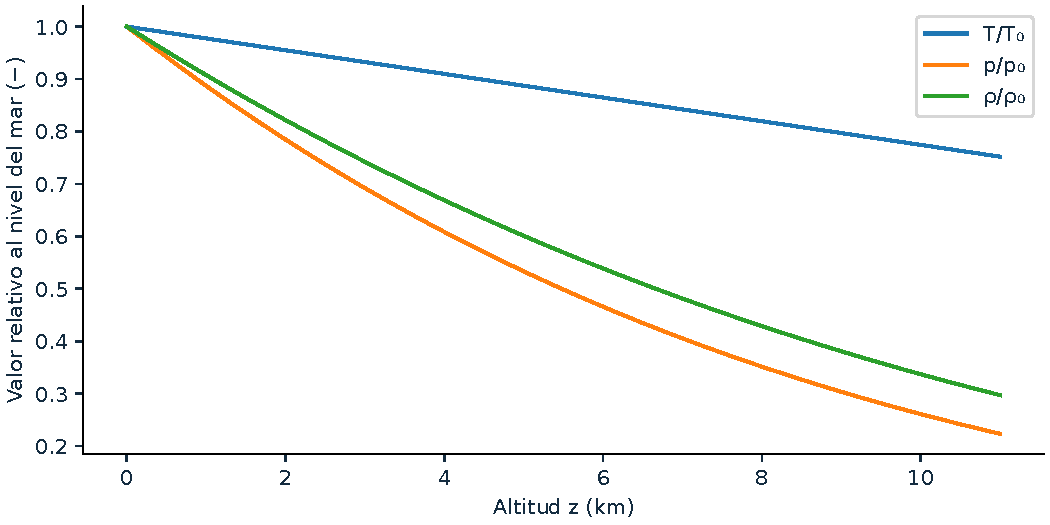
\includegraphics{../figures/FIG-0080/figure.pdf}}%
\count0=\ht0
\advance\count0 by \dp0
\count2=\wd0
\count4=\dimexpr\textheight/100*38\relax
\count6=\linewidth
\ifnum\count0<1
\count0=1
\fi
\ifnum\count2<1
\count2=1
\fi
\divide\count0 by 4096
\divide\count2 by 4096
\divide\count4 by 4096
\divide\count6 by 4096
\ifnum\count0<1
\count0=1
\fi
\ifnum\count2<1
\count2=1
\fi
\ifnum\count4<1
\count4=1
\fi
\ifnum\count6<1
\count6=1
\fi
\count8=\count2
\ifnum\count0>\count4
\count8=\numexpr\count2*\count4/\count0\relax
\fi
\ifnum\count8>\count6
\resizebox{\linewidth}{!}{\box0}%
\else
\ifnum\count0>\count4
\resizebox{!}{\dimexpr\textheight/100*38\relax}{\box0}%
\else
\box0%
\fi
\fi
\endgroup
\par\nopagebreak
\studiumcaption{fig:m01-atmosfera}{Presión, densidad y temperatura de la troposfera estándar, adimensionalizadas con sus valores al nivel del mar, entre 0 y 11 km. Figura exportada por Mathematica 15.0.1 al ejecutar el bloque D de la práctica 1 (companion/m01-fundamentos.wl; SHA-256 bdcd5304ea4a...).}
\end{minipage}
\par\vspace{\baselineskip}

Órdenes de Mathematica. Una asignación con \texttt{=} (Set) evalúa el lado derecho una vez y guarda el resultado; una con \texttt{:=} (SetDelayed) guarda la expresión sin evaluar y la evalúa cada vez que se usa. Por eso las funciones se definen con \texttt{f[x\_] := ...}: el guion bajo declara un patrón, de modo que \texttt{x} toma el valor del argumento en cada llamada. Los argumentos van entre corchetes, las listas entre llaves y los nombres internos empiezan por mayúscula (\texttt{Sin}, \texttt{Pi}, \texttt{D}). \texttt{D[f, z]} deriva, \texttt{Integrate} y \texttt{NIntegrate} integran de forma simbólica y numérica, \texttt{Solve} resuelve ecuaciones algebraicas exactas y \texttt{FindRoot} busca numéricamente una raíz partiendo de un valor inicial. El primer bloque fija los parámetros e ilustra la diferencia entre \texttt{=} y \texttt{:=} con números aleatorios:
\begin{lstlisting}[style=studium]
ClearAll["Global`*"];
g0 = 9.80665;            (* m/s^2, gravedad estandar *)
R = 287.05287;           (* J/(kg K), constante del aire *)
T0 = 288.15; p0 = 101325.; (* K y Pa al nivel del mar *)
lapse = N[-6.5/1000];     (* K/m: -6,5 K por km en la troposfera *)
r1 = RandomReal[];       (* Set (=): se evalua una vez *)
r2 := RandomReal[];      (* SetDelayed (:=): se evalua en cada uso *)
Print["A: r1 dos veces = ", {r1, r1}, "  r2 dos veces distintas = ", Unequal[r2, r2]];
\end{lstlisting}
El segundo define las tres funciones del modelo y comprueba con \texttt{D} y \texttt{Simplify} que la presión cumple la hidrostática; la condición \texttt{0 < z < 11000} informa a \texttt{Simplify} del dominio:
\begin{lstlisting}[style=studium]
temp[z_] := T0 + lapse z;
pres[z_] := p0 (temp[z]/T0)^(-g0/(lapse R));
dens[z_] := pres[z]/(R temp[z]);
Print["B: p(11000) = ", pres[11000.], " Pa,  rho(11000) = ", dens[11000.], " kg/m^3"];
(* Comprobacion: la presion cumple la ecuacion de la hidrostatica (derivada de p mas rho g, nula) *)
hydro = Simplify[D[pres[z], z] + dens[z] g0, 0 < z < 11000];
Print["B: dp/dz + rho g simplificado = ", Chop[hydro]];
\end{lstlisting}

El tercer bloque resuelve una ecuación con \texttt{FindRoot}, integra numéricamente la densidad y resuelve con \texttt{DSolveValue} la atmósfera isoterma, en la que la temperatura no depende de la altitud:
\begin{lstlisting}[style=studium]
zHalf = z /. FindRoot[pres[z] == p0/2, {z, 5000}];
Print["C: altitud con la mitad de la presion = ", zHalf, " m"];
(* Masa de aire por metro cuadrado entre 0 y 11 km, integrando la densidad *)
mCol = NIntegrate[dens[z], {z, 0, 11000}];
Print["C: masa de la columna 0-11 km = ", mCol, " kg/m^2,  (p0 - p(11 km))/g0 = ", (p0 - pres[11000.])/g0];
(* Atmosfera isoterma: solucion simbolica con DSolve *)
iso = DSolveValue[{pp'[z] == -pp[z] g0/(R TT), pp[0] == p0}, pp[z], z];
Print["C: atmosfera isoterma p(z) = ", iso];
\end{lstlisting}
Resultados de la ejecución y verificación. La presión a 11 km es 22 632 Pa y la densidad 0.3639 kg/m\(^3\), valores que coinciden con la tabla de la atmósfera estándar; la presión se reduce a la mitad a 5477 m; y la integral de la densidad entre 0 y 11 km vale 8024.45 kg/m\(^2\), exactamente lo mismo que \((p_0 - p(11\ \mathrm{km}))/g_0\). Esta última coincidencia es una verificación independiente: la diferencia de presión entre dos niveles es el peso por unidad de área del aire que hay entre ellos, de modo que el código y la física se comprueban mutuamente. La comprobación simbólica de la hidrostática devuelve 0, y la atmósfera isoterma resulta exponencial, \(p_0\,e^{-g_0 z/(R T)}\), como debe.

\section{Representación gráfica y exploración interactiva}

Representación gráfica. \texttt{Plot} evalúa una o varias funciones en un intervalo y une los puntos; \texttt{ParametricPlot} dibuja una curva \(\{x(s), y(s)\}\) al variar un parámetro, lo que permite, por ejemplo, poner la altitud en el eje vertical, como en los sondeos meteorológicos. \texttt{Export} guarda la figura en un archivo. \texttt{Manipulate} crea controles deslizantes para explorar un parámetro; solo funciona dentro de un cuaderno, y su resultado se verifica evaluando el cuerpo en valores concretos del control, como hace la última línea:
\begin{lstlisting}[style=studium]
figD = Plot[{pres[z]/p0, dens[z]/dens[0], temp[z]/T0}, {z, 0, 11000},
  PlotLegends -> {"p/p0", "rho/rho0", "T/T0"}, AxesLabel -> {"z (m)", None},
  PlotStyle -> {Black, Blue, Red}, ImageSize -> 400];
Export["figures/m01-atmosfera.png", Rasterize[figD, Background -> White, ImageResolution -> 96]];
figP = ParametricPlot[{pres[z]/1000, z/1000}, {z, 0, 11000}, AspectRatio -> 0.8,
  AxesLabel -> {"p (kPa)", "z (km)"}, PlotStyle -> Blue, ImageSize -> 300];
Export["figures/m01-parametrico.png", Rasterize[figP, Background -> White, ImageResolution -> 96]];
\end{lstlisting}
\begin{lstlisting}[style=studium]
explorar = Manipulate[
  Plot[(1 + a z/T0)^(-g0/(a R)), {z, 0, 11000}, PlotRange -> {0, 1},
    AxesLabel -> {"z (m)", "p/p0"}],
  {{a, -0.0065, "gradiente (K/m)"}, -0.0098, -0.002}];
(* Verificacion sin interfaz: el cuerpo del Manipulate en un valor concreto del control *)
Print["E: p/p0 a 5 km con a = -0.0065: ", (1 + lapse 5000/T0)^(-g0/(lapse R)), " ; con a = -0.0098: ", (1 - 0.0098 5000/T0)^(-g0/(-0.0098 R))];
\end{lstlisting}
La figura~\ref{fig:m01-atmosfera} muestra el resultado: la densidad disminuye más despacio que la presión, porque la temperatura también disminuye y, como la densidad es \(p/(RT)\), compensa en parte la caída de presión: a 11 km la presión es el 22.3 \% de la del nivel del mar y la densidad, el 29.7 \%. Con el control del \texttt{Manipulate} se comprueba que un gradiente térmico más intenso, \(-9.8\) K/km, reduce la presión a 5 km del 53.3 \% al 52.2 \% de la del nivel del mar.

\begin{tcolorbox}[title={Consejo}, studiumtip, breakable]

Errores frecuentes: escribir \texttt{sin(x)} en lugar de \texttt{Sin[x]}; definir una función con \texttt{=} cuando depende de parámetros que cambiarán después; olvidar el guion bajo del patrón; reutilizar un símbolo que ya tiene un valor numérico (empiece cada práctica borrando las definiciones globales, como hace la primera línea de cada guion); y confiar en un resultado numérico sin una comprobación física independiente, como la masa de la columna de aire del bloque C. Un resultado que no se ha comprobado de dos maneras distintas es solo una hipótesis.
\end{tcolorbox}



\section{Desarrollos y práctica}

\begin{tcolorbox}[title={Desarrollos del modelo}, studiumdef, breakable]

\noindent\textbf{Presión de la troposfera estándar como solución de la hidrostática}

\[
T(z) = T_0 + \lambda z,\qquad p(z) = p_0\left(\frac{T(z)}{T_0}\right)^{-g_0/(\lambda R)},\qquad \rho(z) = \frac{p(z)}{R\,T(z)}
\]

\noindent\textbf{Hipótesis}
\begin{itemize}
\item aire seco como gas ideal
\item gradiente térmico lambda constante (troposfera, 0-11 km)
\item gravedad uniforme g0
\end{itemize}

\noindent\textbf{Principios}
\begin{itemize}
\item ecuación de la hidrostática dp/dz = -rho g
\item ecuación de estado p = rho R T
\end{itemize}

\noindent\textbf{Limitaciones}
\begin{itemize}
\item solo para la troposfera; en la estratosfera inferior la temperatura es constante
\end{itemize}

\noindent\textbf{Pasos}
\begin{enumerate}
\item
hidrostática con la ecuación de estado

\[
\frac{dp}{dz} = -\frac{p\,g_0}{R\,(T_0 + \lambda z)}
\]
\item
separar variables e integrar con $T = T_0 + \lambda z$

\[
\ln\frac{p}{p_0} = -\frac{g_0}{\lambda R}\,\ln\frac{T_0 + \lambda z}{T_0}
\]
\item
comprobación: derivar $p(z)$ y sustituir

\[
\frac{dp}{dz} + \rho\,g_0 = 0
\]
\end{enumerate}

\noindent\textbf{Variables}
\begin{itemize}
\item $\lambda$: gradiente térmico vertical ($\mathrm{K}\,\mathrm{m}^{-1}$)
\item $g_{0}$: gravedad estándar ($\mathrm{m}\,\mathrm{s}^{-2}$)
\end{itemize}


\end{tcolorbox}

\begin{tcolorbox}[title={Problema resuelto}, studiumworked, breakable]

\noindent\textbf{Enunciado}

Calcule la presión estática en la tropopausa estándar ($\mathrm{ISA}$, $z = 11\,000\,\mathrm{m}$) a partir de las condiciones al nivel del mar ($p_0 = 101\,325\,\mathrm{Pa}$, $T_0 = 288.15\,\mathrm{K}$), el gradiente térmico troposférico $L = 0.0065\,\mathrm{K\,m^{-1}}$, la constante del aire $R_g = 287.05287\,\mathrm{J\,kg^{-1}\,K^{-1}}$ y la gravedad normal $g_0 = 9.80665\,\mathrm{m\,s^{-2}}$.

\noindent\textbf{Desarrollo paso a paso}

\noindent\textbf{Elección del procedimiento.} La hidrostática da $dp/dz=-\rho g_0$. Sustituyendo $\rho=p/(R_gT)$ y $T=T_0-Lz$, se separa $dp/p=-g_0\,dz/[R_g(T_0-Lz)]$. Integrar desde el nivel del mar da $\ln(p/p_0)=[g_0/(R_gL)]\ln(T/T_0)$. Exponenciar recupera la ley barométrica.

\begin{enumerate}

\item Calcular primero la temperatura en la capa con gradiente.

\[\fitmath{T=T0-L\cdot z}\]

\[\fitmath{T=(288.15)-(0.0065)\cdot (11000)\approx 216.65\,\mathrm{K}}\]

\item El exponente debe ser adimensional.

\[\fitmath{\mathrm{aexp}=\frac{g}{R_g\cdot L}}\]

\[\fitmath{\mathrm{aexp}=\frac{(9.80665)}{(287.05287)\cdot (0.0065)}\approx 5.25588\,}\]

\item Aplicar la potencia al cociente de temperaturas absolutas.

\[\fitmath{p=p0\cdot {\left(\frac{T}{T0}\right)}^{\mathrm{aexp}}}\]

\[\fitmath{p=(101325)\cdot {\left(\frac{(216.65)}{(288.15)}\right)}^{(5.255879813)}\approx 22632.04\,\mathrm{Pa}}\]

\end{enumerate}


\noindent\textbf{Respuesta}

\(p(11\,000\,\mathrm{m}) = 22\,632.04\,\mathrm{Pa}\)
\end{tcolorbox}

\begin{tcolorbox}[title={Ejercicios propuestos}, studiumworked, breakable]

\noindent\textbf{1 (Básico, Cálculo)}
Con las funciones de la práctica 1 (troposfera estándar con gradiente térmico de \(-0.0065\) K/m, 288.15 K y 101 325 Pa al nivel del mar, constante del aire de 287.05287 J/(kg K) y gravedad de 9.80665 m/s\(^2\)), calcule la presión y la densidad a 5000 m. Compruebe el resultado con Mathematica y a mano.
\end{tcolorbox}

\begin{tcolorbox}[title={Autoevaluación}, studiumcheck, breakable]

Ejercicios propuestos. (1) Añada la estratosfera inferior, entre 11 y 20 km, con temperatura constante, y represente \(p(z)\) continua entre 0 y 20 km. (2) Calcule con \texttt{FindRoot} la altitud a la que la densidad es la mitad de la del nivel del mar y explique por qué es mayor que 5477 m. (3) Repita el cálculo de la masa de la columna con \texttt{Integrate} simbólico y compare. (4) Construya un \texttt{Manipulate} que muestre la presión en Marte con \(g = 3.71\) m/s\(^2\) y \(R = 188.9\) J/(kg K). (5) Verifique que la derivada de \texttt{pres} coincide con \(-\rho g_0\) en cinco altitudes elegidas al azar.
\end{tcolorbox}
\studiumchaptercheck

\chapter{Práctica 2. Mecánica clásica y ecuaciones diferenciales}
\label{chap:m02}

\studiumchapterguide{Objetivos: plantear ecuaciones diferenciales ordinarias a partir de un problema mecánico, resolverlas de forma exacta con \texttt{DSolve} cuando existe solución cerrada y numérica con \texttt{NDSolve} cuando no, detener una integración con un suceso (\texttt{WhenEvent}) y, sobre todo, validar una solución numérica con una solución analítica o con una ley de conservación. Los modelos son tres: un proyectil con resistencia aerodinámica cuadrática, el péndulo no lineal y el vehículo a potencia constante del capítulo 1.}

\section{Proyectil con y sin resistencia del aire}

Problema físico. Una pelota de tenis de 57 g y 67 mm de diámetro se lanza a 30 m/s con un ángulo de 40\(^\circ\). Se quiere comparar el alcance en el vacío con el alcance en aire (densidad de 1.2 kg/m\(^3\) y coeficiente de resistencia de 0.55). Sin resistencia, la segunda ley de Newton da dos ecuaciones lineales desacopladas, \(\ddot x = 0\) y \(\ddot y = -g\), que \texttt{DSolve} integra con las cuatro condiciones iniciales; el alcance resultante, 90.35 m, coincide con la fórmula \(v_0^{2}\sin 2\theta/g = 30^2\sin(80^\circ)/9.81 = 90.349\) m:
\begin{lstlisting}[style=studium]
ClearAll["Global`*"];
g = 9.81; v0 = 30.; th = 40 Degree;
solA = DSolve[{x''[t] == 0, y''[t] == -g, x[0] == 0, y[0] == 0,
    x'[0] == v0 Cos[th], y'[0] == v0 Sin[th]}, {x[t], y[t]}, t] // First;
tFlight = t /. Last[Solve[(y[t] /. solA) == 0, t]];
Print["A: x(t), y(t) = ", {x[t], y[t]} /. solA];
Print["A: tiempo de vuelo = ", tFlight, " s, alcance = ", (x[t] /. solA) /. t -> tFlight, " m, formula v0^2 sin(2 th)/g = ", v0^2 Sin[2 th]/g];
\end{lstlisting}
Con resistencia cuadrática la fuerza aerodinámica es \(-k|\mathbf{v}|\mathbf{v}\), con \(k = \rho C_D A/2 = 1.2\cdot 0.55\cdot\pi\cdot 0.067^2/4/2 = 0.0011635\) kg/m, y las ecuaciones quedan acopladas y no lineales, \(m\ddot x = -k|\mathbf{v}|\dot x\) y \(m\ddot y = -mg - k|\mathbf{v}|\dot y\): no tienen solución cerrada y hay que integrarlas numéricamente. \texttt{WhenEvent[Y[t] < 0, ...]} detiene la integración cuando la pelota llega al suelo y guarda ese instante:
\begin{lstlisting}[style=studium]
{m, diam, rho, cd} = {0.057, 0.067, 1.2, 0.55};   (* pelota de tenis *)
kq = rho cd Pi diam^2/4/2;                       (* k = rho Cd A / 2, en kg/m *)
eqs = {X''[t] == -(kq/m) Sqrt[X'[t]^2 + Y'[t]^2] X'[t],
       Y''[t] == -g - (kq/m) Sqrt[X'[t]^2 + Y'[t]^2] Y'[t],
       X[0] == 0, Y[0] == 0, X'[0] == v0 Cos[th], Y'[0] == v0 Sin[th],
       WhenEvent[Y[t] < 0, tImpact = t; "StopIntegration"]};
solB = NDSolve[eqs, {X, Y}, {t, 0, 10}] // First;
Print["B: k = ", kq, " kg/m, tiempo de vuelo = ", tImpact, " s, alcance con resistencia = ", X[tImpact] /. solB, " m"];
figB = Show[ParametricPlot[{x[t], y[t]} /. solA, {t, 0, tFlight}, PlotStyle -> {Dashed, Black}],
   ParametricPlot[{X[t], Y[t]} /. solB, {t, 0, tImpact}, PlotStyle -> Blue],
   AxesLabel -> {"x (m)", "y (m)"}, PlotRange -> All, AspectRatio -> 0.45, ImageSize -> 420];
Export["figures/m02-proyectil.png", Rasterize[figB, Background -> White, ImageResolution -> 96]];
(* Verificacion: la energia mecanica debe disminuir monotonamente con resistencia *)
energia[t_] := (1/2) m (X'[t]^2 + Y'[t]^2) + m g Y[t] /. solB;
Print["B: energia inicial y final (J) = ", {energia[0], energia[tImpact]}, ", trabajo disipado = ", energia[0] - energia[tImpact]];
\end{lstlisting}

\par\vspace{\baselineskip}
\noindent\begin{minipage}{\linewidth}
\centering
\begingroup
\setbox0=\hbox{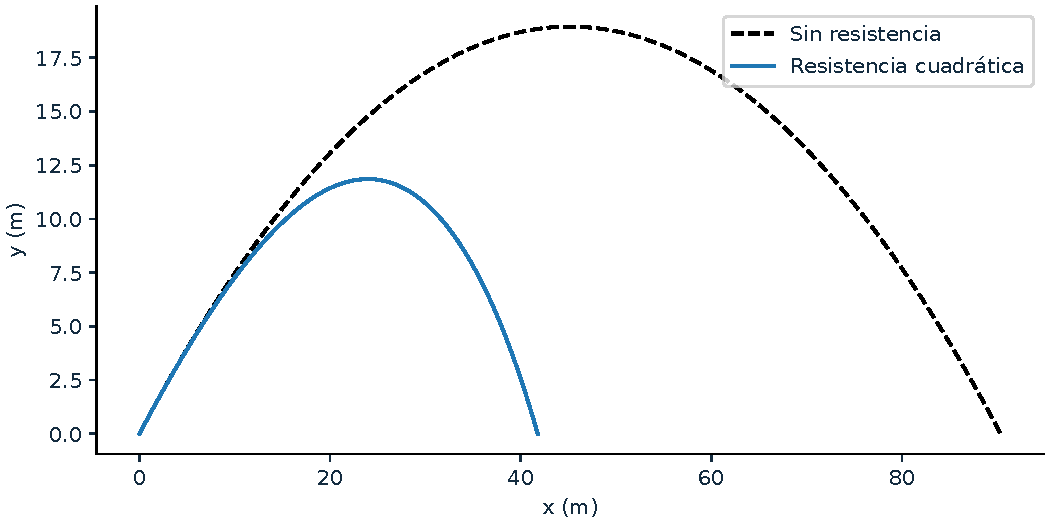
\includegraphics{../figures/FIG-0081/figure.pdf}}%
\count0=\ht0
\advance\count0 by \dp0
\count2=\wd0
\count4=\dimexpr\textheight/100*38\relax
\count6=\linewidth
\ifnum\count0<1
\count0=1
\fi
\ifnum\count2<1
\count2=1
\fi
\divide\count0 by 4096
\divide\count2 by 4096
\divide\count4 by 4096
\divide\count6 by 4096
\ifnum\count0<1
\count0=1
\fi
\ifnum\count2<1
\count2=1
\fi
\ifnum\count4<1
\count4=1
\fi
\ifnum\count6<1
\count6=1
\fi
\count8=\count2
\ifnum\count0>\count4
\count8=\numexpr\count2*\count4/\count0\relax
\fi
\ifnum\count8>\count6
\resizebox{\linewidth}{!}{\box0}%
\else
\ifnum\count0>\count4
\resizebox{!}{\dimexpr\textheight/100*38\relax}{\box0}%
\else
\box0%
\fi
\fi
\endgroup
\par\nopagebreak
\studiumcaption{fig:m02-proyectil}{Trayectorias de una pelota de tenis lanzada a 30 m/s y 40\(^\circ\): en el vacío (discontinua, alcance 90.3 m) y con resistencia cuadrática (azul, alcance 41.8 m). Redibujada vectorialmente a partir de las ecuaciones de esta práctica; véase el registro de figuras reproducibles.}
\end{minipage}
\par\vspace{\baselineskip}

\par\vspace{\baselineskip}
\noindent\begin{minipage}{\linewidth}
\centering
\begingroup
\setbox0=\hbox{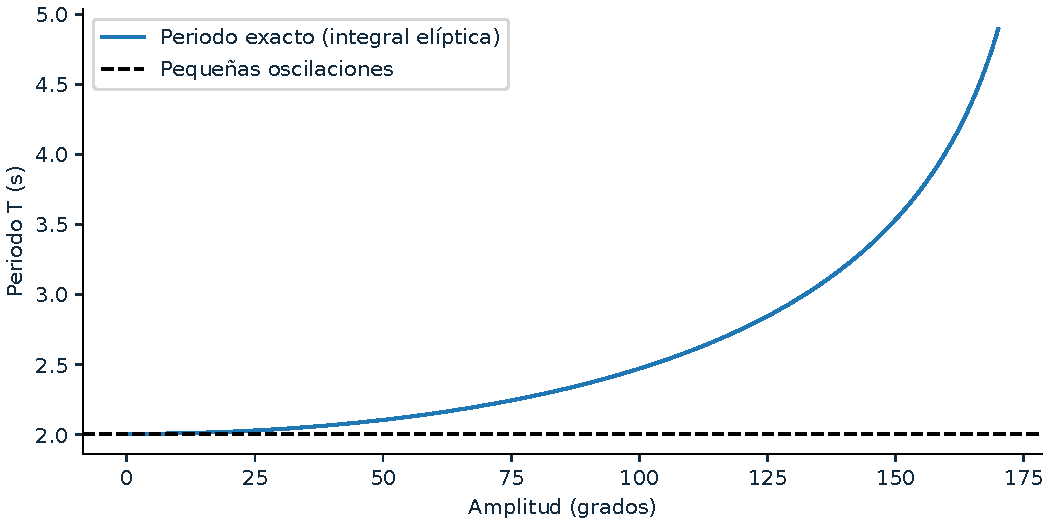
\includegraphics{../figures/FIG-0082/figure.pdf}}%
\count0=\ht0
\advance\count0 by \dp0
\count2=\wd0
\count4=\dimexpr\textheight/100*38\relax
\count6=\linewidth
\ifnum\count0<1
\count0=1
\fi
\ifnum\count2<1
\count2=1
\fi
\divide\count0 by 4096
\divide\count2 by 4096
\divide\count4 by 4096
\divide\count6 by 4096
\ifnum\count0<1
\count0=1
\fi
\ifnum\count2<1
\count2=1
\fi
\ifnum\count4<1
\count4=1
\fi
\ifnum\count6<1
\count6=1
\fi
\count8=\count2
\ifnum\count0>\count4
\count8=\numexpr\count2*\count4/\count0\relax
\fi
\ifnum\count8>\count6
\resizebox{\linewidth}{!}{\box0}%
\else
\ifnum\count0>\count4
\resizebox{!}{\dimexpr\textheight/100*38\relax}{\box0}%
\else
\box0%
\fi
\fi
\endgroup
\par\nopagebreak
\studiumcaption{fig:m02-periodo}{Periodo del péndulo de 1 m frente a la amplitud: fórmula exacta con la integral elíptica (azul), periodo lineal (discontinua) y valores obtenidos con NDSolve y WhenEvent (puntos rojos). Redibujada vectorialmente a partir de las ecuaciones de esta práctica; véase el registro de figuras reproducibles.}
\end{minipage}
\par\vspace{\baselineskip}

Resultados e interpretación. El tiempo de vuelo baja de 3.93 s a 3.09 s y el alcance de 90.3 m a 41.8 m: para una pelota ligera a 30 m/s la resistencia no es una corrección, sino el efecto dominante. La trayectoria deja de ser simétrica: la rama descendente es más empinada que la ascendente (figura~\ref{fig:m02-proyectil}). La comprobación física es la energía: debe disminuir monótonamente, y la diferencia entre la energía inicial (25.65 J) y la final (6.84 J) es el trabajo de la resistencia, 18.8 J. Una solución numérica cuya energía aumentara indicaría un error de signo en la fuerza aerodinámica, el error más frecuente al escribir estas ecuaciones.

\section{Péndulo: solución analítica y numérica}

El péndulo simple de longitud \(L\) obedece \(\ddot\theta = -\omega_0^{2}\sin\theta\), con \(\omega_0 = \sqrt{g/L}\). Para amplitudes pequeñas, \(\sin\theta \approx \theta\) y \texttt{DSolve} da la oscilación armónica de periodo \(2\pi/\omega_0\), 2.006 s para \(L = 1\) m. Para amplitudes finitas la integral de la energía conduce a un periodo exacto en términos de la integral elíptica completa \(K\), \(T = 4K(\sin^{2}(\theta_0/2))/\omega_0\), que Mathematica evalúa con \texttt{EllipticK}. La práctica obtiene el periodo de dos formas independientes: con la fórmula exacta y con \texttt{NDSolve}, registrando con \texttt{WhenEvent} los pasos de \(\theta\) por cero, que están separados medio periodo:
\begin{lstlisting}[style=studium]
L = 1.0; w0 = Sqrt[g/L];
lin = DSolveValue[{q''[t] + w0^2 q[t] == 0, q[0] == q0, q'[0] == 0}, q[t], t];
Print["C: solucion lineal = ", lin, ", periodo lineal = ", 2 Pi/w0, " s"];
periodo[amp_?NumericQ] := Module[{qq, tc = {}},
   NDSolve[{qq''[t] + w0^2 Sin[qq[t]] == 0, qq[0] == amp, qq'[0] == 0,
      WhenEvent[qq[t] == 0, AppendTo[tc, t]]}, qq, {t, 0, 20}, MaxStepSize -> 0.005];
   2 (tc[[2]] - tc[[1]])];                       (* dos pasos por cero consecutivos = medio periodo *)
periodoExacto[amp_] := 4 EllipticK[Sin[amp/2]^2]/w0;
Print["C: periodo a 90 grados: NDSolve = ", periodo[N[Pi/2]], " s, integral eliptica = ", N[periodoExacto[Pi/2]], " s"];
Print["C: periodo a 10 grados: NDSolve = ", periodo[N[10 Degree]], " s, lineal = ", 2 Pi/w0, " s"];
figC = Plot[{periodoExacto[a Degree], 2 Pi/w0}, {a, 1, 170}, PlotStyle -> {Blue, {Dashed, Black}},
   AxesLabel -> {"amplitud (grados)", "T (s)"}, PlotRange -> {0, 6}, ImageSize -> 400,
   Epilog -> {Red, PointSize[0.015], Point[{#, periodo[N[# Degree]]} & /@ {30, 60, 90, 120, 150}]}];
Export["figures/m02-periodo.png", Rasterize[figC, Background -> White, ImageResolution -> 96]];
(* Conservacion de la energia como comprobacion del integrador *)
solC = NDSolve[{p''[t] + w0^2 Sin[p[t]] == 0, p[0] == Pi/2, p'[0] == 0}, p, {t, 0, 20}] // First;
en[t_] := (1/2) p'[t]^2 + w0^2 (1 - Cos[p[t]]) /. solC;
Print["C: deriva relativa maxima de la energia en 20 s = ", Max[Table[Abs[(en[t] - en[0])/en[0]], {t, 0, 20, 0.01}]]];
\end{lstlisting}
Para 90\(^\circ\) ambos métodos dan 2.36784 s (difieren en \(10^{-9}\) s), un 18 \% más que el periodo lineal; para 10\(^\circ\) el periodo es 2.0099 s, solo un 0.19 \% mayor que el lineal (figura~\ref{fig:m02-periodo}). La deriva relativa de la energía en 20 s de integración es \(7\times 10^{-7}\): el integrador conserva la energía con la precisión pedida. La comparación entre la solución numérica y la exacta, y la conservación de la energía, son las dos verificaciones que deben acompañar a toda solución obtenida con \texttt{NDSolve}.

El último bloque enlaza con la familia de problemas del capítulo 1: el ciclista a potencia constante obedece \(M\dot V = P/V - Mg\sin\varphi - k_D V^{2}\). \texttt{FindRoot} da la velocidad máxima, 6.083 m/s, la misma del ejemplo del capítulo 1, y \texttt{NDSolve} muestra que, partiendo de 1 m/s, el ciclista tarda 20.2 s en alcanzar el 95 \% de ella. Ese tiempo no se puede obtener con el razonamiento de régimen estacionario: es la parte de la física que solo la ecuación diferencial contiene.
\begin{lstlisting}[style=studium]
M = 85; P = 250; phi = ArcTan[0.04]; kd = 0.5 rho 0.35;
vmax = v /. FindRoot[P/v - M g Sin[phi] - kd v^2 == 0, {v, 5}];
solD = NDSolve[{M V'[t] == P/V[t] - M g Sin[phi] - kd V[t]^2, V[0] == 1,
    WhenEvent[V[t] > 0.95 vmax, t95 = t]}, V, {t, 0, 200}] // First;
Print["D: velocidad maxima = ", vmax, " m/s, tiempo hasta el 95 % partiendo de 1 m/s = ", t95, " s"];
\end{lstlisting}

\begin{tcolorbox}[title={Consejo}, studiumtip, breakable]

Errores frecuentes con \texttt{NDSolve}: dar menos condiciones iniciales que el orden de las ecuaciones; escribir \texttt{y[t]''} en lugar de \texttt{y''[t]}; olvidar que la solución es una función interpolada válida solo en el intervalo de integración; usar \texttt{WhenEvent} con una condición que ya se cumple en el instante inicial; y no comprobar nunca la solución con una ley de conservación o con un caso límite conocido. La práctica hace las dos cosas en cada modelo para que se convierta en un hábito.
\end{tcolorbox}



\section{Desarrollos y práctica}

\begin{tcolorbox}[title={Desarrollos del modelo}, studiumdef, breakable]

\noindent\textbf{Periodo del péndulo simple de amplitud finita}

\begin{equation}
T(\theta_0) = \frac{4}{\omega_0}\,K\!\left(\sin^{2}\frac{\theta_0}{2}\right),\qquad \omega_0 = \sqrt{g/L},\qquad T(\theta_0) \to \frac{2\pi}{\omega_0}\ (\theta_0 \to 0)
\label{eq:m02-periodo}
\end{equation}

\noindent\textbf{Hipótesis}
\begin{itemize}
\item péndulo ideal: varilla sin masa, sin rozamiento
\item gravedad uniforme
\end{itemize}

\noindent\textbf{Principios}
\begin{itemize}
\item conservación de la energía mecánica
\item segunda ley de Newton en dirección tangencial
\end{itemize}

\noindent\textbf{Limitaciones}
\begin{itemize}
\item K es una función especial: la comprobación numérica la hace Mathematica (EllipticK) y la práctica la contrasta con NDSolve
\end{itemize}

\noindent\textbf{Pasos}
\begin{enumerate}
\item
ecuación del movimiento

\[
\ddot\theta + \omega_0^{2}\sin\theta = 0
\]
\item
integral primera de la energía

\[
\tfrac12\dot\theta^{2} + \omega_0^{2}(1 - \cos\theta) = \omega_0^{2}(1 - \cos\theta_0)
\]
\item
periodo como integral; K es la integral elíptica completa de primera especie con parámetro m = sin\(^2(\)theta0/2)

\[
T = \frac{4}{\omega_0}\,K\!\left(\sin^{2}\frac{\theta_0}{2}\right)
\]
\item
límite de pequeñas oscilaciones: K(0) = pi/2

\[
T = \frac{4}{\omega_0}\cdot\frac{\pi}{2} = \frac{2\pi}{\omega_0}
\]
\end{enumerate}

\noindent\textbf{Variables}
\begin{itemize}
\item $\omega_0$: pulsación de pequeñas oscilaciones ($\mathrm{1/s}$)
\item $\theta_0$: amplitud angular ($\mathrm{rad}$)
\end{itemize}


\end{tcolorbox}

\begin{tcolorbox}[title={Problema resuelto}, studiumworked, breakable]

\noindent\textbf{Enunciado}

Determine el alcance horizontal en el vacío de un proyectil lanzado desde el suelo con velocidad inicial $v_0 = 30\,\mathrm{m\,s^{-1}}$ y ángulo de tiro $\theta_0 = 40^{\circ}$ sobre la horizontal ($g = 9.81\,\mathrm{m\,s^{-2}}$) como referencia previa al análisis con resistencia cuadrática.

\noindent\textbf{Desarrollo paso a paso}

\noindent\textbf{Elección del procedimiento.} Separar componentes: $\ddot x=0$, $\ddot y=-g$. Con origen en el lanzamiento se obtiene $x=v_0\cos\theta\,t$ e $y=v_0\sin\theta\,t-gt^2/2$. Imponer $y=0$ da dos raíces: $t=0$ y el regreso al suelo; se elige la segunda positiva.

\begin{enumerate}

\item La componente horizontal permanece constante en el vacío.

\[\fitmath{\mathrm{vx}=v_{0}\cdot \cos\left(\theta\right)}\]

\[\fitmath{\mathrm{vx}=(30)\cdot \cos\left((0.6981317008)\right)\approx 22.98133\,\mathrm{m/s}}\]

\item La componente vertical inicial fija el tiempo de vuelo.

\[\fitmath{\mathrm{vy}=v_{0}\cdot \sin\left(\theta\right)}\]

\[\fitmath{\mathrm{vy}=(30)\cdot \sin\left((0.6981317008)\right)\approx 19.28363\,\mathrm{m/s}}\]

\item Dividir $t(v_{y0}-gt/2)=0$ por la raíz inicial ya identificada.

\[\fitmath{\mathrm{tf}=\frac{2\cdot \mathrm{vy}}{g}}\]

\[\fitmath{\mathrm{tf}=\frac{2\cdot (19.28362829)}{(9.81)}\approx 3.931423\,\mathrm{s}}\]

\item Introducir ese tiempo en $x(t)$; equivale a $v_0^2\sin(2\theta)/g$.

\[\fitmath{R=\mathrm{vx}\cdot \mathrm{tf}}\]

\[\fitmath{R=(22.98133329)\cdot (3.931422689)\approx 90.34934\,\mathrm{m}}\]

\end{enumerate}


\noindent\textbf{Respuesta}

\(x_{\max} = 90.349\,\mathrm{m}\)
\end{tcolorbox}

\begin{tcolorbox}[title={Ejercicios propuestos}, studiumworked, breakable]

\noindent\textbf{1 (Intermedio, Cálculo)}
Un péndulo simple de 1.0 m se suelta desde el reposo con una amplitud de 90\(^\circ\) (\(g = 9.81\) m/s\(^2\)). (a) Calcule el periodo de pequeñas oscilaciones. (b) Con la práctica 2, el periodo exacto resulta ser \(T = 4K(1/2)/\omega_0\) con \(K(1/2) = 1.8540747\). Calcúlelo y obtenga el porcentaje en que supera al periodo lineal.
\end{tcolorbox}

\begin{tcolorbox}[title={Autoevaluación}, studiumcheck, breakable]

Ejercicios propuestos. (1) Encuentre con \texttt{NDSolve} y \texttt{FindMaximum} el ángulo de lanzamiento que maximiza el alcance con resistencia y compárelo con 45\(^\circ\). (2) Añada un viento horizontal constante y explique por qué la fuerza aerodinámica depende de la velocidad relativa al aire. (3) Para el péndulo, represente \(\theta(t)\) lineal y no lineal para 120\(^\circ\) y mida el desfase al cabo de cinco periodos. (4) Añada al péndulo un amortiguamiento viscoso \(c\dot\theta\) y compruebe que la energía disminuye. (5) Para el ciclista, compare el tiempo hasta el 95 \% de la velocidad máxima en subida y en bajada.
\end{tcolorbox}
\studiumchaptercheck

\chapter{Práctica 3. Cinemática de fluidos}
\label{chap:m03}

\studiumchapterguide{Objetivos: obtener un campo de velocidad a partir de una función de corriente; calcular de forma simbólica el tensor gradiente de velocidad, la aceleración material, la vorticidad y la fuerza por unidad de volumen; visualizar el campo con líneas de corriente y curvas \(\psi = \) constante; y distinguir líneas de corriente y trayectorias en un flujo no estacionario. La práctica automatiza exactamente el método de cinco pasos del capítulo 12, de modo que el alumno puede comprobar sus cálculos a mano de los problemas de la familia de la función de corriente.}

\section{Derivada material, gradientes y vorticidad}

Problema y modelo. Se parte de un campo plano prescrito, matemáticamente incompresible pero no necesariamente solución de Navier--Stokes sin fuerzas de volumen, del ejemplo resuelto del capítulo 12, \(\psi = K\,(x^{2}y + 2xy^{2})\) con \(K = 1\) m\(^{-1}\)s\(^{-1}\), en agua. La velocidad es \((\partial\psi/\partial y,\ -\partial\psi/\partial x)\); \texttt{Div} comprueba la continuidad, \texttt{Grad} aplicado a la lista de componentes devuelve la matriz de derivadas \(\partial u_i/\partial x_j\) y el producto matricial de esa matriz por la velocidad (el punto, \texttt{.}) da la aceleración convectiva, como en la forma matricial del capítulo 4. \texttt{Curl} de un campo plano devuelve el escalar \(\partial v/\partial x - \partial u/\partial y\):
\begin{lstlisting}[style=studium]
ClearAll["Global`*"];
K = 1;                                        (* 1/(m s) *)
psi = K (x^2 y + 2 x y^2);
vel = {D[psi, y], -D[psi, x]};
Print["A: velocidad = ", vel, ", divergencia = ", Simplify[Div[vel, {x, y}]]];
\end{lstlisting}
\begin{lstlisting}[style=studium]
gradV = Grad[vel, {x, y}];                     (* matriz d u_i / d x_j *)
acc = Simplify[gradV . vel];                   (* aceleracion convectiva (flujo estacionario) *)
vort = Curl[vel, {x, y}];                      (* escalar en 2D: dv/dx - du/dy *)
lamb = Simplify[Grad[(vel . vel)/2, {x, y}] - vort {vel[[2]], -vel[[1]]}];
Print["B: aceleracion = ", Factor[acc], ", vorticidad = ", vort];
Print["B: forma de Lamb igual a la convectiva: ", Simplify[lamb == acc]];
pt = {x -> 1, y -> 2}; {rho} = {1000};
Print["B: en (1,2): u = ", vel /. pt, ", a = ", acc /. pt, ", fuerza por unidad de volumen = ", rho acc /. pt, ", modulo = ", N[Norm[rho acc /. pt]]];
Print["B: laplaciano de u = ", Laplacian[#, {x, y}] & /@ vel, " ; -rot(omega) = ", {-D[vort, y], D[vort, x]}];
\end{lstlisting}

\par\vspace{\baselineskip}
\noindent\begin{minipage}{\linewidth}
\centering
\begingroup
\setbox0=\hbox{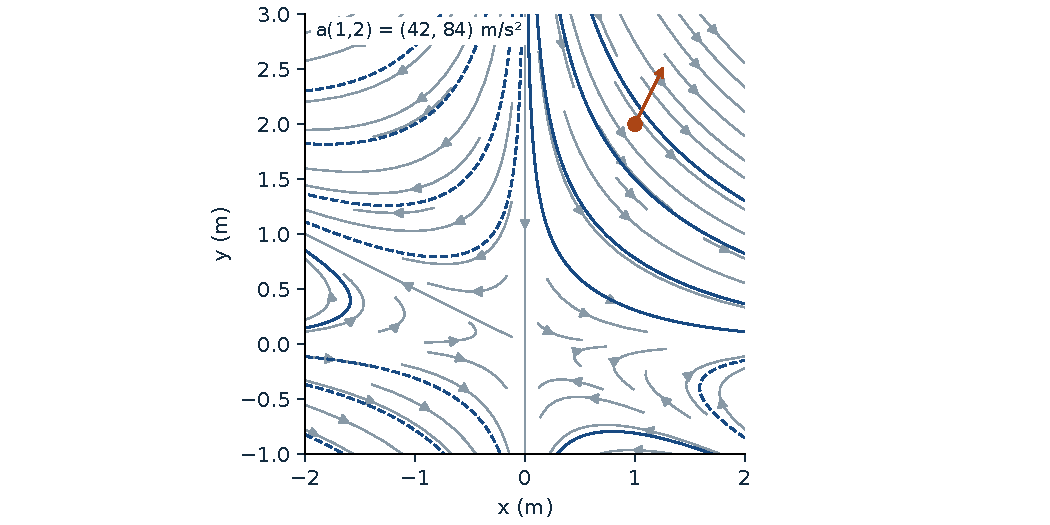
\includegraphics{../figures/FIG-0083/figure.pdf}}%
\count0=\ht0
\advance\count0 by \dp0
\count2=\wd0
\count4=\dimexpr\textheight/100*38\relax
\count6=\linewidth
\ifnum\count0<1
\count0=1
\fi
\ifnum\count2<1
\count2=1
\fi
\divide\count0 by 4096
\divide\count2 by 4096
\divide\count4 by 4096
\divide\count6 by 4096
\ifnum\count0<1
\count0=1
\fi
\ifnum\count2<1
\count2=1
\fi
\ifnum\count4<1
\count4=1
\fi
\ifnum\count6<1
\count6=1
\fi
\count8=\count2
\ifnum\count0>\count4
\count8=\numexpr\count2*\count4/\count0\relax
\fi
\ifnum\count8>\count6
\resizebox{\linewidth}{!}{\box0}%
\else
\ifnum\count0>\count4
\resizebox{!}{\dimexpr\textheight/100*38\relax}{\box0}%
\else
\box0%
\fi
\fi
\endgroup
\par\nopagebreak
\studiumcaption{fig:m03-corriente}{Campo \(\psi = x^{2}y + 2xy^{2}\) (en m\(^2\)/s con \(K = 1\)): líneas de corriente de StreamPlot (gris) y curvas \(\psi = \) constante de ContourPlot (azul), que coinciden; la flecha roja es la aceleración en \((1, 2)\), \((42;\ 84)\) m/s\(^2\), a escala. Redibujada vectorialmente a partir de las ecuaciones de esta práctica; véase el registro de figuras reproducibles.}
\end{minipage}
\par\vspace{\baselineskip}

Resultados verificados. Mathematica devuelve la velocidad \((x^{2} + 4xy,\ -2xy - 2y^{2})\), divergencia nula, la aceleración factorizada \(2(x^{2} + 2xy + 4y^{2})\,(x,\ y)\) y la vorticidad \(-4x - 2y\), idénticas a las del capítulo 12. En el punto \((1, 2)\) la velocidad es \((9;\ -12)\) m/s, la aceleración \((42;\ 84)\) m/s\(^2\) y la fuerza neta por unidad de volumen \((42\,000;\ 84\,000)\) N/m\(^3\), de módulo 93 915 N/m\(^3\). La línea que compara la forma de Lamb, \(\nabla(|\mathbf{u}|^{2}/2) - \mathbf{u}\times\boldsymbol{\omega}\), con la aceleración convectiva devuelve \texttt{True}: es una verificación simbólica en todo el plano, no solo en un punto. Por último, el laplaciano de la velocidad vale \((2;\ -4)\) y coincide con menos el rotacional de la vorticidad, la identidad que usa el capítulo 14 para el término viscoso. La verificación simbólica de continuidad, vorticidad y aceleración no equivale a validar el campo como solución física estacionaria: véase la prueba de incompatibilidad del gradiente de presión en el capítulo 14.

\section{Campos de velocidad, líneas de corriente y trayectorias}

Visualización. \texttt{StreamPlot} dibuja líneas tangentes al campo de velocidad en cada punto, y \texttt{ContourPlot} de \(\psi\) dibuja sus curvas de nivel; en un flujo plano estacionario ambas familias son las mismas curvas, y superponerlas es una comprobación visual del signo de la velocidad. La flecha roja representa la aceleración en \((1, 2)\), dirigida hacia fuera del origen (figura~\ref{fig:m03-corriente}):
\begin{lstlisting}[style=studium]
figC = Show[
   StreamPlot[vel, {x, -2, 2}, {y, -2, 3}, StreamColorFunction -> None, StreamStyle -> Gray, StreamPoints -> Coarse],
   ContourPlot[psi, {x, -2, 2}, {y, -2, 3}, Contours -> {-6, -3, -1, 1, 3, 6, 10}, ContourShading -> None, ContourStyle -> Blue],
   Graphics[{Red, PointSize[0.02], Point[{1, 2}], Arrow[{{1, 2}, {1, 2} + (acc /. pt)/150}]}],
   FrameLabel -> {"x (m)", "y (m)"}, ImageSize -> 360];
Export["figures/m03-corriente.png", Rasterize[figC, Background -> White, ImageResolution -> 72]];
\end{lstlisting}
En un flujo no estacionario líneas de corriente y trayectorias son distintas. Para el campo \(u = u_0\), \(v = a t\) del capítulo 4, las líneas de corriente en cada instante son rectas de pendiente \(a t/u_0\), mientras que la trayectoria de una partícula es una parábola. \texttt{NDSolveValue} integra la trayectoria, \(\dot X = u\), \(\dot Y = v\), y la comparación con la solución analítica \((u_0 t,\ a t^{2}/2)\) en \(t = 4\) s da \((8;\ 4)\) m con un error de \(3\times 10^{-9}\) m:
\begin{lstlisting}[style=studium]
u0 = 2; a = 0.5;                               (* u = u0, v = a t (capitulo 4) *)
tray = NDSolveValue[{X'[t] == u0, Y'[t] == a t, X[0] == 0, Y[0] == 0}, {X[t], Y[t]}, {t, 0, 4}];
Print["D: trayectoria en t = 4 s: ", tray /. t -> 4., ", analitica {u0 t, a t^2/2} = ", {u0 4, a 16/2}];
pendiente[t_] := a t/u0;                       (* las lineas de corriente en el instante t son rectas *)
Print["D: pendiente de las lineas de corriente en t = 2 s = ", pendiente[2], ", de la trayectoria en ese instante = ", (a t/u0) /. t -> 2];
figD = Show[ParametricPlot[tray, {t, 0, 4}, PlotStyle -> Blue],
   Plot[pendiente[4] xx, {xx, 0, 8}, PlotStyle -> {Dashed, Black}],
   AxesLabel -> {"x (m)", "y (m)"}, PlotRange -> {{0, 8}, {0, 8}}, AspectRatio -> 0.6, ImageSize -> 360];
Export["figures/m03-trayectoria.png", Rasterize[figD, Background -> White, ImageResolution -> 72]];
\end{lstlisting}

\begin{tcolorbox}[title={Consejo}, studiumtip, breakable]

Errores frecuentes: olvidar el signo menos de \(v = -\partial\psi/\partial x\); aplicar \texttt{Grad} a un escalar cuando se quería el gradiente de cada componente (el resultado tiene otra forma); escribir el producto de matriz por vector con un espacio (producto elemento a elemento) en lugar del punto; y evaluar en el punto antes de derivar. Compruebe siempre que la divergencia es nula y que la forma de Lamb coincide con la aceleración.
\end{tcolorbox}



\section{Desarrollos y práctica}

\begin{tcolorbox}[title={Ejercicios propuestos}, studiumworked, breakable]

\noindent\textbf{1 (Intermedio, Desarrollo)}
Adapte la práctica 3 al campo \(\psi = K\,(x^{3} - 3xy^{2})\) con \(K = 0.50\) m\(^{-1}\)s\(^{-1}\). (a) Compruebe con Mathematica que el flujo es incompresible e irrotacional. (b) Calcule la aceleración de la partícula que pasa por \((1, 2)\) m y su módulo. (c) Explique por qué la aceleración es en este caso el gradiente de \(|\mathbf{u}|^{2}/2\).
\end{tcolorbox}

\begin{tcolorbox}[title={Autoevaluación}, studiumcheck, breakable]

Ejercicios propuestos. (1) Repita la práctica para \(\psi = K\,(x^{3} - 3xy^{2})\) y compruebe que la vorticidad es nula. (2) Calcule la fuerza por unidad de volumen del problema no estacionario del capítulo 12 añadiendo \texttt{D[vel, t]} a la aceleración. (3) Dibuje con \texttt{VectorPlot} el campo de aceleraciones del ejemplo y explique su simetría. (4) Calcule la traza de partículas emitidas desde el origen en el campo \(u = u_0\), \(v = a t\) y compárela con la trayectoria y con la línea de corriente en \(t = 4\) s.
\end{tcolorbox}
\studiumchaptercheck

\chapter{Práctica 4. Bernoulli y volúmenes de control}
\label{chap:m04}

\studiumchapterguide{Objetivos: combinar continuidad y Bernoulli en cálculos paramétricos; resolver la ecuación diferencial del vaciado de un depósito de forma exacta y numérica y elegir la rama físicamente correcta; integrar la distribución de presión sobre un cuerpo para obtener fuerzas; y aplicar un balance de cantidad de movimiento a un volumen de control. Todos los modelos proceden del capítulo 12 y del capítulo 9.}

\section{Continuidad y Bernoulli en conductos y depósitos}

Medidor Venturi. Con continuidad, \(V_1 A_1 = V_2 A_2\), y Bernoulli entre la entrada y la garganta se obtiene el caudal en función de la diferencia de presión medida y de la relación de diámetros \(\beta = d_2/d_1\):
\begin{equation}
Q = A_2\,\sqrt{\frac{2\,\Delta p}{\rho\,(1 - \beta^{4})}}. \label{eq:m04-venturi}
\end{equation}
La función \texttt{caudal} de la práctica implementa esta expresión; \texttt{Solve} la invierte para obtener la diferencia de presión que corresponde a un caudal dado, y un \texttt{Plot} con varias curvas resume el estudio paramétrico:
\begin{lstlisting}[style=studium]
ClearAll["Global`*"];
{rho, d1, d2} = {998., 0.100, 0.050};
area[d_] := Pi d^2/4;
caudal[dp_, beta_] := area[beta d1] Sqrt[2 dp/(rho (1 - beta^4))];
Print["A: Q para dp = 20 kPa y beta = 0.5: ", caudal[20000., 0.5], " m^3/s"];
dpNecesaria = dp /. Solve[caudal[dp, 0.5] == 0.020, dp][[1]];
Print["A: dp necesaria para Q = 20 l/s: ", dpNecesaria, " Pa"];
figA = Plot[Evaluate[Table[1000 caudal[dp, b], {b, {0.4, 0.5, 0.6, 0.7}}]], {dp, 0, 40000},
   PlotLegends -> {"d2/d1: 0.4", "0.5", "0.6", "0.7"}, AxesLabel -> {"dp (Pa)", "Q (l/s)"}, ImageSize -> 400];
Export["figures/m04-venturi.png", Rasterize[figA, Background -> White, ImageResolution -> 96]];
\end{lstlisting}
Para agua, un diámetro de entrada de 100 mm, una relación de diámetros de 0.5 y 20 kPa el caudal es 0.012838 m\(^3\)/s (12.8 l/s), y para medir 20 l/s hacen falta 48.5 kPa: como \(Q \propto \sqrt{\Delta p}\), aumentar el caudal en un 56 \% exige multiplicar la diferencia de presión por 2.4. El gráfico (figura~\ref{fig:m04-venturi}) muestra por qué se eligen gargantas más estrechas para caudales pequeños: dan más diferencia de presión, y por tanto más resolución, para el mismo caudal.

\par\vspace{\baselineskip}
\noindent\begin{minipage}{\linewidth}
\centering
\begingroup
\setbox0=\hbox{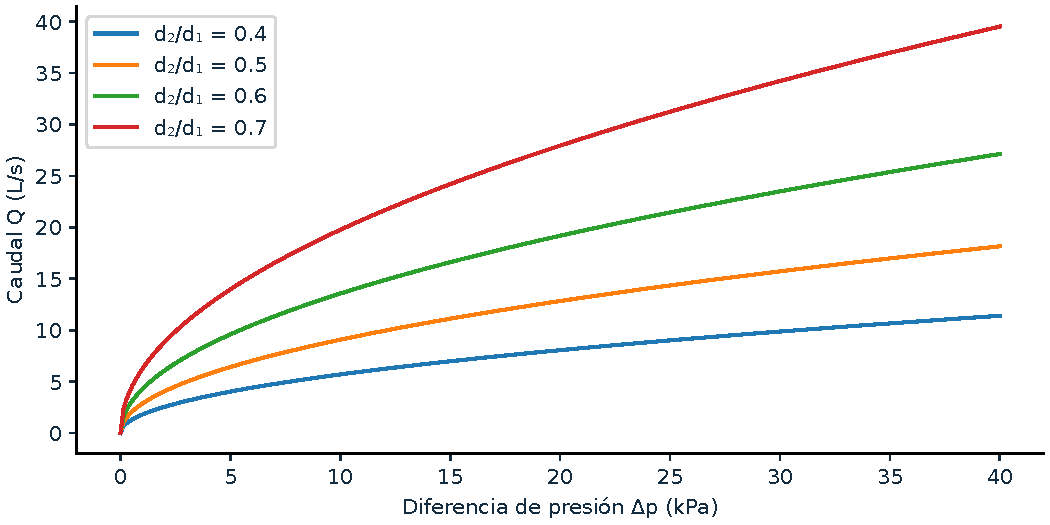
\includegraphics{../figures/FIG-0084/figure.pdf}}%
\count0=\ht0
\advance\count0 by \dp0
\count2=\wd0
\count4=\dimexpr\textheight/100*38\relax
\count6=\linewidth
\ifnum\count0<1
\count0=1
\fi
\ifnum\count2<1
\count2=1
\fi
\divide\count0 by 4096
\divide\count2 by 4096
\divide\count4 by 4096
\divide\count6 by 4096
\ifnum\count0<1
\count0=1
\fi
\ifnum\count2<1
\count2=1
\fi
\ifnum\count4<1
\count4=1
\fi
\ifnum\count6<1
\count6=1
\fi
\count8=\count2
\ifnum\count0>\count4
\count8=\numexpr\count2*\count4/\count0\relax
\fi
\ifnum\count8>\count6
\resizebox{\linewidth}{!}{\box0}%
\else
\ifnum\count0>\count4
\resizebox{!}{\dimexpr\textheight/100*38\relax}{\box0}%
\else
\box0%
\fi
\fi
\endgroup
\par\nopagebreak
\studiumcaption{fig:m04-venturi}{Caudal de agua de un Venturi ideal de 100 mm frente a la diferencia de presión para cuatro relaciones de diámetros. Redibujada vectorialmente a partir de las ecuaciones de esta práctica; véase el registro de figuras reproducibles.}
\end{minipage}
\par\vspace{\baselineskip}

\par\vspace{\baselineskip}
\noindent\begin{minipage}{\linewidth}
\centering
\begingroup
\setbox0=\hbox{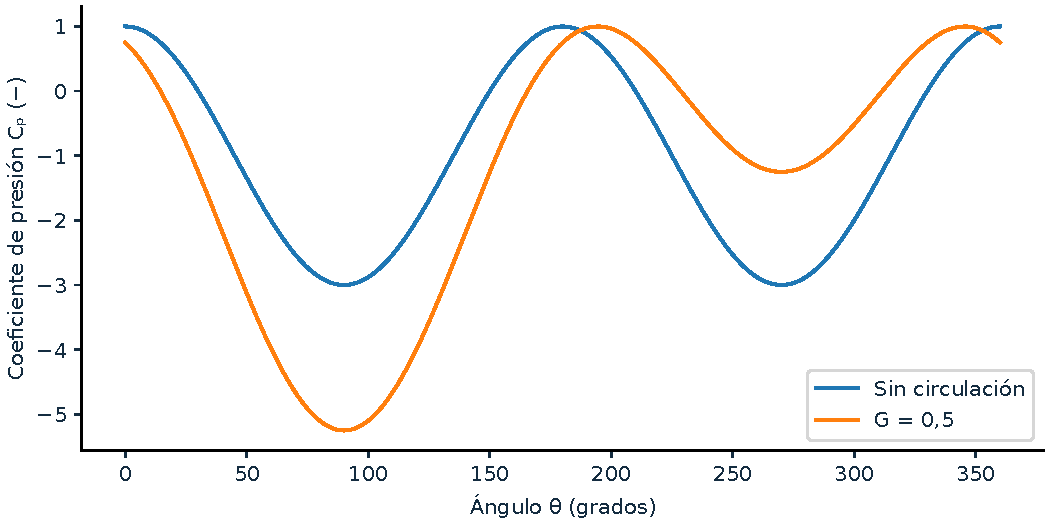
\includegraphics{../figures/FIG-0085/figure.pdf}}%
\count0=\ht0
\advance\count0 by \dp0
\count2=\wd0
\count4=\dimexpr\textheight/100*38\relax
\count6=\linewidth
\ifnum\count0<1
\count0=1
\fi
\ifnum\count2<1
\count2=1
\fi
\divide\count0 by 4096
\divide\count2 by 4096
\divide\count4 by 4096
\divide\count6 by 4096
\ifnum\count0<1
\count0=1
\fi
\ifnum\count2<1
\count2=1
\fi
\ifnum\count4<1
\count4=1
\fi
\ifnum\count6<1
\count6=1
\fi
\count8=\count2
\ifnum\count0>\count4
\count8=\numexpr\count2*\count4/\count0\relax
\fi
\ifnum\count8>\count6
\resizebox{\linewidth}{!}{\box0}%
\else
\ifnum\count0>\count4
\resizebox{!}{\dimexpr\textheight/100*38\relax}{\box0}%
\else
\box0%
\fi
\fi
\endgroup
\par\nopagebreak
\studiumcaption{fig:m04-cilindro}{Coeficiente de presión sobre un cilindro en flujo potencial frente al ángulo, sin circulación (negro) y con \(G = \Gamma/(2\pi R U) = 0.5\) (azul). Redibujada vectorialmente a partir de las ecuaciones de esta práctica; véase el registro de figuras reproducibles.}
\end{minipage}
\par\vspace{\baselineskip}

Vaciado de un depósito. Un depósito de sección \(A = 0.50\) m\(^2\) con agua hasta \(h_0 = 2.0\) m se vacía por un orificio de \(a = 10\) cm\(^2\). Combinando el balance de masa del depósito con la velocidad de Torricelli, \(\sqrt{2gh}\), resulta \(dh/dt = -(a/A)\sqrt{2gh}\). \texttt{DSolve} devuelve dos ramas, porque al elevar al cuadrado aparece la solución espuria en la que el nivel sube; la rama física es \(h(t) = (\sqrt{h_0} - (a/A)\sqrt{g/2}\,t)^{2}\), válida hasta el vaciado, en \(t_v = (A/a)\sqrt{2h_0/g} = 319.28\) s. El código sustituye la rama física en la ecuación y comprueba que el residuo es nulo, y después resuelve el mismo problema con \texttt{NDSolve}, deteniéndolo con \texttt{WhenEvent} cuando quedan 1 mm de agua:
\begin{lstlisting}[style=studium]
g = 9.81; At = 0.50; ao = 0.0010; h0 = 2.0;
sols = DSolve[{h'[t] == -(ao/At) Sqrt[2 g h[t]], h[0] == h0}, h[t], t];  (* dos ramas: hay que elegir *)
hAn[t_] := (Sqrt[h0] - (ao/At) Sqrt[g/2] t)^2;   (* rama fisica: el nivel baja desde h0 *)
tVac = (At/ao) Sqrt[2 h0/g];
Print["B: ramas de DSolve = ", Length[sols], ", residuo de la rama fisica = ", Simplify[hAn'[t] + (ao/At) Sqrt[2 g hAn[t]], 0 < t < tVac], ", tiempo de vaciado analitico = ", tVac, " s"];
Print["B: tiempo analitico hasta h = 1 mm = ", (At/ao) Sqrt[2/g] (Sqrt[h0] - Sqrt[0.001]), " s"];
num = NDSolve[{H'[t] == -(ao/At) Sqrt[2 g Max[H[t], 0]], H[0] == h0,
    WhenEvent[H[t] < 0.001, tEnd = t; "StopIntegration"]}, H, {t, 0, 2000}];
Print["B: tiempo hasta h = 1 mm con NDSolve = ", tEnd, " s"];
\end{lstlisting}
El instante numérico, 312.13622 s, coincide con el analítico para \(h = 1\) mm, 312.13621 s, en las siete primeras cifras. Elegir la rama correcta de una solución simbólica y contrastarla con una integración numérica son hábitos que evitan errores difíciles de detectar.

\section{Distribución de presión en flujo potencial}

Presión sobre un cilindro y fuerzas. En el flujo potencial alrededor de un cilindro con circulación, la velocidad en la superficie da un coeficiente de presión \(C_p(\theta) = 1 - (2\sin\theta + G)^{2}\), con \(G = \Gamma/(2\pi R U)\). Las fuerzas por unidad de longitud son integrales de la presión sobre el contorno, y \texttt{Integrate} las calcula de forma simbólica para cualquier \(G\):
\begin{lstlisting}[style=studium]
cp[th_, G_] := 1 - (2 Sin[th] + G)^2;          (* G = Gamma/(2 pi R U) *)
drag[G_] := -Integrate[cp[th, G] Cos[th], {th, 0, 2 Pi}]/2;   (* coeficiente por unidad de longitud y de diametro *)
lift[G_] := -Integrate[cp[th, G] Sin[th], {th, 0, 2 Pi}]/2;
Print["C: Cd(G) = ", Simplify[drag[G]], ", Cl(G) = ", Simplify[lift[G]], " (Kutta-Joukowski: Cl = 2 pi G)"];
figC = Plot[{cp[th Degree, 0], cp[th Degree, 0.5]}, {th, 0, 360}, AxesLabel -> {"theta (grados)", "Cp"},
   PlotLegends -> {"sin circulacion", "G = 0.5"}, PlotStyle -> {Black, Blue}, ImageSize -> 400];
Export["figures/m04-cilindro.png", Rasterize[figC, Background -> White, ImageResolution -> 96]];
\end{lstlisting}
El resultado, resistencia nula y un coeficiente de sustentación igual a \(2\pi G\), reproduce la paradoja de D'Alembert (sin viscosidad no hay resistencia) y el teorema de Kutta-Joukowski (la sustentación es proporcional a la circulación). La figura~\ref{fig:m04-cilindro} muestra cómo la circulación rompe la simetría de la distribución de presión entre la parte superior y la inferior.

Balance de cantidad de movimiento. Un chorro de agua de 5 l/s a 20 m/s que un álabe desvía un ángulo \(\beta\) sin pérdidas ejerce sobre él, en la dirección del chorro, una fuerza \(\rho Q V(1 - \cos\beta)\): el flujo de cantidad de movimiento que entra menos la componente del que sale. Para 90\(^\circ\), 120\(^\circ\) y 180\(^\circ\) resultan 99.8 N, 149.7 N y 199.6 N; con 120\(^\circ\), \(998\cdot 0.005\cdot 20\cdot(1 - \cos 120^\circ) = 149.70\) N. La inversión completa del chorro duplica la fuerza respecto de la placa plana, que es el principio de las turbinas Pelton:
\begin{lstlisting}[style=studium]
V = 20.; Q = 0.005;
fuerza[beta_] := rho Q V (1 - Cos[beta]);
Print["D: fuerza para desvio de 90, 120 y 180 grados: ", fuerza /@ {90 Degree, 120 Degree, 180 Degree}, " N"];
\end{lstlisting}

\begin{tcolorbox}[title={Consejo}, studiumtip, breakable]

Antes de aplicar Bernoulli en un cálculo automático, compruebe sus hipótesis: flujo estacionario, incompresible, sin pérdidas y a lo largo de una línea de corriente. Cuando \texttt{DSolve} devuelva varias soluciones, no tome la primera: sustituya cada una en las condiciones físicas del problema. Y compare siempre un resultado numérico con un caso que pueda calcular a mano.
\end{tcolorbox}



\section{Desarrollos y práctica}

\begin{tcolorbox}[title={Desarrollos del modelo}, studiumdef, breakable]

\noindent\textbf{Caudal de un medidor Venturi ideal}

\[
Q = A_2\,\sqrt{\frac{2\,\Delta p}{\rho\,(1 - \beta^{4})}},\qquad \beta = \frac{d_2}{d_1}
\]

\noindent\textbf{Hipótesis}
\begin{itemize}
\item flujo estacionario, incompresible y sin pérdidas
\item velocidad uniforme en cada sección
\end{itemize}

\noindent\textbf{Principios}
\begin{itemize}
\item continuidad
\item ecuación de Bernoulli entre la entrada y la garganta
\end{itemize}

\noindent\textbf{Limitaciones}
\begin{itemize}
\item un Venturi real necesita un coeficiente de descarga algo menor que 1
\end{itemize}

\noindent\textbf{Pasos}
\begin{enumerate}
\item
continuidad entre la entrada y la garganta

\[
V_1 A_1 = V_2 A_2 \;\Rightarrow\; V_1 = \beta^{2} V_2
\]
\item
Bernoulli entre ambas secciones

\[
\Delta p = p_1 - p_2 = \tfrac12\rho\,(V_2^{2} - V_1^{2})
\]
\item
eliminar V1 y despejar el caudal

\[
V_2 = \sqrt{\frac{2\,\Delta p}{\rho\,(1 - \beta^{4})}}
\]
\end{enumerate}

\noindent\textbf{Variables}
\begin{itemize}
\item $\beta$: relación de diámetros
\item $A_{2}$: área de la garganta ($\mathrm{m}^{2}$)
\end{itemize}



\noindent\textbf{Vaciado de un depósito por un orificio (Torricelli cuasiestacionario)}

\begin{equation}
\frac{dh}{dt} = -\frac{a}{A}\sqrt{2gh},\qquad h(t) = \left(\sqrt{h_0} - \frac{a}{A}\sqrt{\frac{g}{2}}\;t\right)^{2},\qquad t_v = \frac{A}{a}\sqrt{\frac{2h_0}{g}}
\label{eq:m04-vaciado}
\end{equation}

\noindent\textbf{Hipótesis}
\begin{itemize}
\item velocidad de salida de Torricelli en cada instante (flujo cuasiestacionario)
\item orificio pequeño frente a la sección del depósito
\item sin pérdidas
\end{itemize}

\noindent\textbf{Principios}
\begin{itemize}
\item conservación de la masa en el depósito
\item Bernoulli entre la superficie libre y el chorro
\end{itemize}

\noindent\textbf{Limitaciones}
\begin{itemize}
\item sin coeficiente de descarga; un orificio real vacía más despacio
\end{itemize}

\noindent\textbf{Pasos}
\begin{enumerate}
\item
balance de masa del depósito

\[
A\,\frac{dh}{dt} = -a\sqrt{2gh}
\]
\item
separar variables e integrar

\[
\sqrt{h} = \sqrt{h_0} - \frac{a}{A}\sqrt{\frac{g}{2}}\;t
\]
\item
tiempo para h = 0

\[
t_v = \frac{A}{a}\sqrt{\frac{2h_0}{g}}
\]
\end{enumerate}

\noindent\textbf{Variables}
\begin{itemize}
\item $a$: área del orificio ($\mathrm{m}^{2}$)
\item $A$: área del depósito ($\mathrm{m}^{2}$)
\end{itemize}


\end{tcolorbox}

\begin{tcolorbox}[title={Problema resuelto}, studiumworked, breakable]

\noindent\textbf{Enunciado}

Un medidor de Venturi horizontal por el que circula agua ($\rho = 998\,\mathrm{kg\,m^{-3}}$) tiene diámetro de garganta $d_2 = 0.05\,\mathrm{m}$ y relación de diámetros $\beta = d_2/d_1 = 0.5$. Si la caída de presión estática entre la entrada y la garganta es $\Delta p = 20\,000\,\mathrm{Pa}$, calcule el caudal volumétrico ideal.

\noindent\textbf{Desarrollo paso a paso}

\noindent\textbf{Elección del procedimiento.} La continuidad da $A_1V_1=A_2V_2$ y, por tanto, $V_1=\beta^2V_2$. Bernoulli horizontal sin pérdidas da $\Delta p=\rho(V_2^2-V_1^2)/2=\rho V_2^2(1-\beta^4)/2$. Despejar primero velocidad y después multiplicar por el área de garganta.

\begin{enumerate}

\item El diámetro determina el área de garganta.

\[\fitmath{A_{2}=\frac{\pi\cdot {d_{2}}^{2}}{4}}\]

\[\fitmath{A_{2}=\frac{\pi\cdot {(0.05)}^{2}}{4}\approx 0.001963495\,\mathrm{m^{2}}}\]

\item Tomar la raíz positiva del balance de energía.

\[\fitmath{V_{2}=\sqrt{\frac{2\cdot \mathrm{dp}}{\rho\cdot \left(1-{\beta}^{4}\right)}}}\]

\[\fitmath{V_{2}=\sqrt{\frac{2\cdot (20000)}{(998)\cdot \left(1-{(0.5)}^{4}\right)}}\approx 6.538514\,\mathrm{m/s}}\]

\item Aplicar $Q=A_2V_2$ en la misma sección.

\[\fitmath{Q=A_{2}\cdot V_{2}}\]

\[\fitmath{Q=(0.001963495408)\cdot (6.538514434)\approx 0.01283834\,\mathrm{m^{3}/s}}\]

\end{enumerate}


\noindent\textbf{Respuesta}

\(Q = 0.012838\,\mathrm{m^{3}\,s^{-1}}\)
\end{tcolorbox}

\begin{tcolorbox}[title={Ejercicios propuestos}, studiumworked, breakable]

\noindent\textbf{1 (Intermedio, Desarrollo)}
Un depósito cilíndrico de 0.50 m\(^2\) de sección contiene agua hasta 2.0 m y se vacía por un orificio de 10 cm\(^2\) sin pérdidas. (a) Plantee la ecuación diferencial del nivel. (b) Obtenga el tiempo de vaciado completo. (c) ¿Qué fracción del tiempo total se emplea en vaciar la mitad inferior de la altura?
\end{tcolorbox}

\begin{tcolorbox}[title={Autoevaluación}, studiumcheck, breakable]

Ejercicios propuestos. (1) Añada al Venturi un coeficiente de descarga de 0.98 y recalcule la diferencia de presión para 20 l/s. (2) Modifique el vaciado para un depósito cónico, cuya sección depende de \(h\), y compare el tiempo de vaciado con el del cilíndrico de igual volumen. (3) Busque con \texttt{Solve} los puntos de remanso del cilindro con circulación y represéntelos frente a \(G\). (4) Calcule la fuerza de un chorro sobre un álabe que se mueve a 8 m/s en el sentido del chorro.
\end{tcolorbox}
\studiumchaptercheck

\chapter{Práctica 5. Flujos viscosos}
\label{chap:m05}

\studiumchapterguide{Objetivos: resolver con \texttt{DSolve} problemas de contorno de flujos viscosos unidireccionales; obtener de la solución el caudal, el esfuerzo en la pared, el par y la potencia; tomar límites con \texttt{Limit}; comprobar con una integral simbólica que la disipación viscosa es igual a la potencia aportada; y validar la solución exacta con una solución numérica independiente. Los modelos son los de los capítulos 6 y 14 y cubren la familia de problemas de cilindros giratorios.}

\section{Couette y Poiseuille: perfiles y esfuerzos}

Couette con gradiente de presión. La ecuación \(\mu\,u'' = -G\) con \(u(0) = 0\) y \(u(h) = U\) es un problema de contorno que \texttt{DSolveValue} resuelve directamente; la práctica obtiene a partir del perfil el caudal por unidad de anchura (con \texttt{Integrate}), el esfuerzo en la placa fija (derivando) y, con \texttt{Solve}, el gradiente de presión adverso que anula ese esfuerzo, \(G = -2\mu U/h^{2}\), umbral del flujo inverso del capítulo 6. Sustituyendo \(y = \eta h\) y \(G = 2\mu U P/h^{2}\) se obtiene el perfil adimensional \(\eta\,(1 + P - P\eta)\), que la figura~\ref{fig:m05-couette} representa para cinco valores de \(P\); en un cuaderno, un \texttt{Manipulate} sobre \(P\) permite ver la aparición del flujo inverso:
\begin{lstlisting}[style=studium]
ClearAll["Global`*"];
perfil = DSolveValue[{mu u''[y] == -G, u[0] == 0, u[h] == U}, u[y], y];
Print["A: u(y) = ", Simplify[perfil]];
q = Integrate[perfil, {y, 0, h}];
tauPared = mu D[perfil, y] /. y -> 0;
Print["A: caudal por unidad de anchura = ", Simplify[q], ", esfuerzo en y = 0: ", Simplify[tauPared]];
Print["A: gradiente que anula el esfuerzo en la placa fija: G = ", G /. Solve[tauPared == 0, G][[1]]];
adim = Simplify[perfil/U /. {y -> eta h, G -> 2 mu U P/h^2}];
Print["A: perfil adimensional u/U = ", adim];
figA = Plot[Evaluate[Table[adim, {P, {-2, -1, 0, 1, 2}}]], {eta, 0, 1}, PlotLegends -> {"P=-2", "P=-1", "P=0", "P=1", "P=2"},
   AxesLabel -> {"y/h", "u/U"}, ImageSize -> 400];
Export["figures/m05-couette.png", Rasterize[figA, Background -> White, ImageResolution -> 96]];
(* En un cuaderno: Manipulate[Plot[adim, {eta, 0, 1}, PlotRange -> {-0.5, 1.6}], {P, -3, 3}] *)
\end{lstlisting}

\par\vspace{\baselineskip}
\noindent\begin{minipage}{\linewidth}
\centering
\begingroup
\setbox0=\hbox{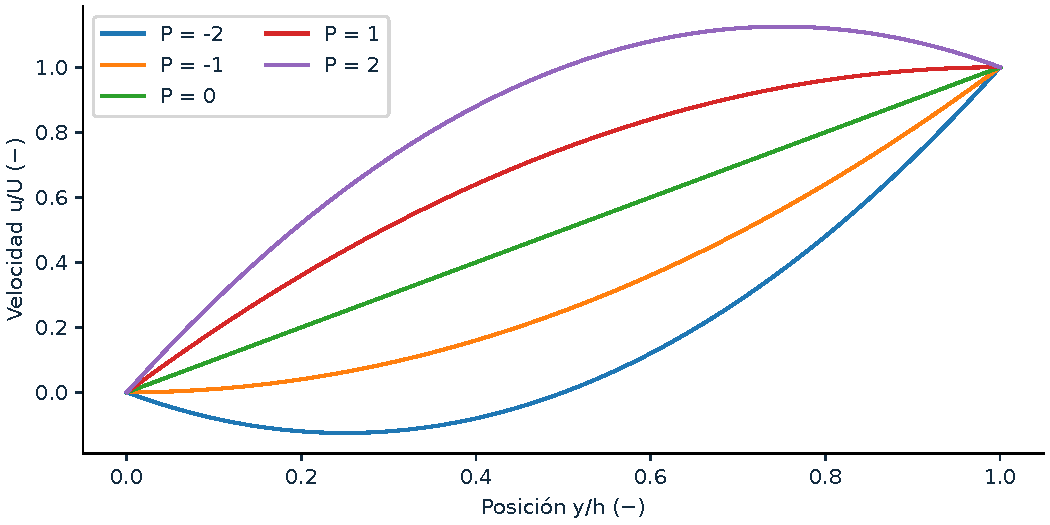
\includegraphics{../figures/FIG-0086/figure.pdf}}%
\count0=\ht0
\advance\count0 by \dp0
\count2=\wd0
\count4=\dimexpr\textheight/100*38\relax
\count6=\linewidth
\ifnum\count0<1
\count0=1
\fi
\ifnum\count2<1
\count2=1
\fi
\divide\count0 by 4096
\divide\count2 by 4096
\divide\count4 by 4096
\divide\count6 by 4096
\ifnum\count0<1
\count0=1
\fi
\ifnum\count2<1
\count2=1
\fi
\ifnum\count4<1
\count4=1
\fi
\ifnum\count6<1
\count6=1
\fi
\count8=\count2
\ifnum\count0>\count4
\count8=\numexpr\count2*\count4/\count0\relax
\fi
\ifnum\count8>\count6
\resizebox{\linewidth}{!}{\box0}%
\else
\ifnum\count0>\count4
\resizebox{!}{\dimexpr\textheight/100*38\relax}{\box0}%
\else
\box0%
\fi
\fi
\endgroup
\par\nopagebreak
\studiumcaption{fig:m05-couette}{Perfiles adimensionales \(u/U = \eta(1 + P - P\eta)\) del flujo de Couette con gradiente de presión para \(P = -2, -1, 0, 1, 2\), obtenidos con DSolve. Redibujada vectorialmente a partir de las ecuaciones de esta práctica; véase el registro de figuras reproducibles.}
\end{minipage}
\par\vspace{\baselineskip}

\par\vspace{\baselineskip}
\noindent\begin{minipage}{\linewidth}
\centering
\begingroup
\setbox0=\hbox{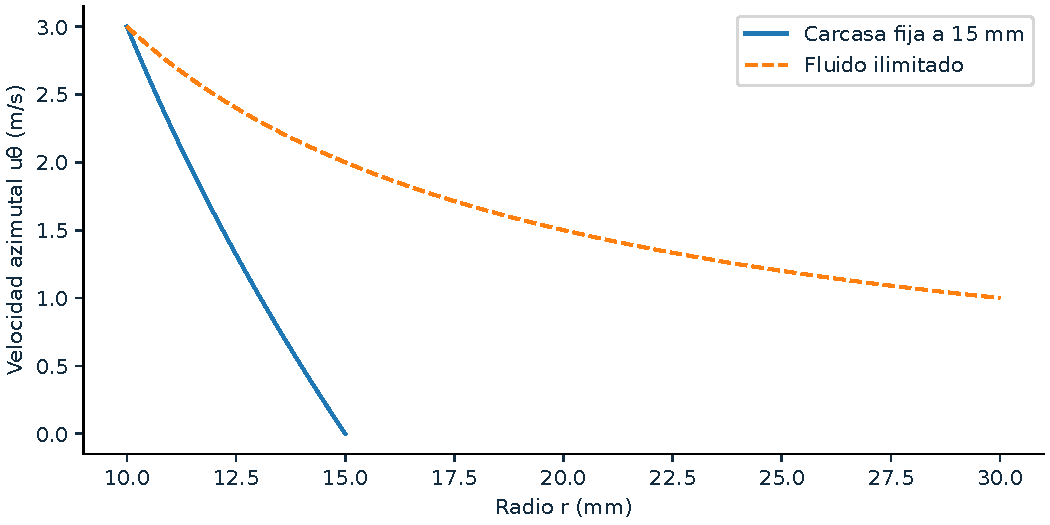
\includegraphics{../figures/FIG-0087/figure.pdf}}%
\count0=\ht0
\advance\count0 by \dp0
\count2=\wd0
\count4=\dimexpr\textheight/100*38\relax
\count6=\linewidth
\ifnum\count0<1
\count0=1
\fi
\ifnum\count2<1
\count2=1
\fi
\divide\count0 by 4096
\divide\count2 by 4096
\divide\count4 by 4096
\divide\count6 by 4096
\ifnum\count0<1
\count0=1
\fi
\ifnum\count2<1
\count2=1
\fi
\ifnum\count4<1
\count4=1
\fi
\ifnum\count6<1
\count6=1
\fi
\count8=\count2
\ifnum\count0>\count4
\count8=\numexpr\count2*\count4/\count0\relax
\fi
\ifnum\count8>\count6
\resizebox{\linewidth}{!}{\box0}%
\else
\ifnum\count0>\count4
\resizebox{!}{\dimexpr\textheight/100*38\relax}{\box0}%
\else
\box0%
\fi
\fi
\endgroup
\par\nopagebreak
\studiumcaption{fig:m05-cilindros}{Velocidad azimutal alrededor de un eje de 10 mm que gira a 300 rad/s: con una carcasa fija a 15 mm (azul, flujo de Couette circular) y en un fluido ilimitado (rojo discontinuo, \(u_\theta = \Omega R^{2}/r\)). Redibujada vectorialmente a partir de las ecuaciones de esta práctica; véase el registro de figuras reproducibles.}
\end{minipage}
\par\vspace{\baselineskip}

\section{Cilindros giratorios: par y potencia disipada}

Cilindros giratorios. La componente azimutal de Navier-Stokes, \(u'' + u'/r - u/r^{2} = 0\), con el no deslizamiento en \(R_1\) y \(R_2\), se resuelve de forma simbólica para radios y velocidades angulares cualesquiera. A partir de la solución, el código construye el esfuerzo \(\mu\,r\,d(u/r)/dr\), el par del motor por unidad de longitud y la función de disipación, y comprueba tres resultados de los capítulos 6 y 14: el par \(4\pi\mu(\Omega_1 - \Omega_2)R_1^{2}R_2^{2}/(R_2^{2} - R_1^{2})\); su límite para un fluido ilimitado, \(4\pi\mu\Omega_1 R_1^{2}\), calculado con \texttt{Limit}; y la igualdad entre la disipación integrada en la corona y la potencia neta de los cilindros, que \texttt{Simplify} reduce a cero:
\begin{lstlisting}[style=studium]
ec = v''[r] + v'[r]/r - v[r]/r^2 == 0;
vSol = DSolveValue[{ec, v[R1] == W1 R1, v[R2] == W2 R2}, v[r], r];
Print["B: u_theta(r) = ", Simplify[vSol]];
tau[r_] = mu r D[vSol/r, r];
par = Simplify[-2 Pi R1^2 tau[R1]];             (* par del motor sobre el cilindro interior, por unidad de longitud *)
Print["B: par por unidad de longitud = ", par];
Print["B: limite fluido ilimitado (R2 -> oo, cilindro exterior en reposo): ", Limit[par /. W2 -> 0, R2 -> Infinity]];
(* Comprobacion energetica: disipacion integrada = potencia neta de los cilindros *)
phi[r_] = tau[r]^2/mu;
disip = Simplify[Integrate[phi[r] 2 Pi r, {r, R1, R2}, Assumptions -> 0 < R1 < R2]];
Print["B: disipacion - (W1 - W2) par = ", Simplify[disip - (W1 - W2) par]];
\end{lstlisting}
Las tres comprobaciones son simbólicas, válidas para cualquier valor de los parámetros: el balance de energía confirma a la vez la solución, el esfuerzo en coordenadas cilíndricas y la expresión del par.

Ejemplo numérico y verificación independiente. Para el eje de 10 mm que gira a 300 rad/s en glicerina del capítulo 14, la potencia por unidad de longitud en un fluido ilimitado es 159.47 W/m; con una carcasa a 15 mm sube a 287.04 W/m, porque el factor \(R_2^{2}/(R_2^{2} - R_1^{2})\) vale 1.8. Para comprobar la solución exacta por un camino distinto, el bloque C resuelve el mismo problema de contorno con \texttt{NDSolveValue} y mide la diferencia máxima entre ambas soluciones, \(5\times 10^{-8}\) m/s, del orden de la tolerancia numérica:
\begin{lstlisting}[style=studium]
datos = {mu -> 1.41, W1 -> 300., R1 -> 0.010, W2 -> 0};
potIlim = 4 Pi mu W1^2 R1^2 /. datos;
Print["C: potencia por unidad de longitud en fluido ilimitado = ", potIlim, " W/m"];
Print["C: con carcasa a R2 = 15 mm: ", W1 par /. datos /. R2 -> 0.015, " W/m"];
(* Verificacion numerica independiente: resolver el problema de contorno con NDSolve *)
num = NDSolveValue[{v''[r] + v'[r]/r - v[r]/r^2 == 0, v[0.010] == 3., v[0.015] == 0}, v, {r, 0.010, 0.015}];
an = vSol /. {R1 -> 0.010, R2 -> 0.015, W1 -> 300., W2 -> 0};
Print["C: error maximo NDSolve frente a la solucion exacta = ", Max[Table[Abs[num[rr] - (an /. r -> rr)], {rr, 0.010, 0.015, 0.0001}]], " m/s"];
figC = Plot[Evaluate[{If[rr <= 0.015, an /. r -> rr, Undefined], 3. 0.010/rr}], {rr, 0.010, 0.030}, PlotStyle -> {Blue, {Dashed, Red}},
   AxesLabel -> {"r (m)", "u_theta (m/s)"}, PlotLegends -> {"carcasa en 15 mm", "fluido ilimitado"}, ImageSize -> 400];
Export["figures/m05-cilindros.png", Rasterize[figC, Background -> White, ImageResolution -> 96]];
\end{lstlisting}
La figura~\ref{fig:m05-cilindros} compara los dos perfiles: con la carcasa la velocidad cae a cero en 5 mm, y los gradientes, el par y la potencia son mayores.

\begin{tcolorbox}[title={Consejo}, studiumtip, breakable]

Errores frecuentes: escribir el esfuerzo como \texttt{mu D[v, r]} en lugar de \texttt{mu r D[v/r, r]}; olvidar el signo al pasar del esfuerzo sobre el fluido al par del motor; pedir a \texttt{Limit} el límite antes de dejar en reposo el cilindro exterior; y aplicar el resultado laminar sin comprobar el número de Reynolds de rotación ni la estabilidad (torbellinos de Taylor). La comprobación energética del bloque B detecta de una vez los tres primeros errores.
\end{tcolorbox}



\section{Desarrollos y práctica}

\begin{tcolorbox}[title={Ejercicios propuestos}, studiumworked, breakable]

\noindent\textbf{1 (Avanzado, PARAMETER\_STUDY)}
Con la expresión del par de la práctica 5, el par sobre un eje que gira dentro de una carcasa fija supera al del mismo eje en un fluido ilimitado en el factor \(R_2^{2}/(R_2^{2} - R_1^{2})\). (a) Deduzca ese factor. (b) Determine la relación de radios \(R_2/R_1\) a partir de la cual el exceso es menor que el 5 \%. (c) Discuta qué significa para un ensayo en un depósito real.
\end{tcolorbox}

\begin{tcolorbox}[title={Autoevaluación}, studiumcheck, breakable]

Ejercicios propuestos. (1) Obtenga con \texttt{DSolve} el perfil de Hagen-Poiseuille en coordenadas cilíndricas, \(\frac{1}{r}\frac{d}{dr}(r\,u') = -G/\mu\), imponiendo velocidad finita en el eje. (2) Calcule la potencia disipada por unidad de anchura en el flujo de Couette-Poiseuille y compruebe que es igual al trabajo de la placa más el del gradiente de presión. (3) Haga girar los dos cilindros en el mismo sentido y busque los valores de \(\Omega_2/\Omega_1\) para los que el par se anula. (4) Represente el par frente a \(R_2/R_1\) y determine a partir de qué relación de radios el error de suponer un fluido ilimitado es menor que el 5 \%.
\end{tcolorbox}
\studiumchaptercheck

\chapter{Práctica 6. Análisis dimensional}
\label{chap:m06}

\studiumchapterguide{Objetivos: automatizar el teorema Pi con la matriz dimensional y su espacio nulo; comprobar la homogeneidad dimensional con cantidades con unidades; ajustar una correlación adimensional a datos experimentales; y predecir el resultado de un ensayo modificado, distinguiendo la predicción por semejanza exacta de la que exige interpolar o usar una correlación. El caso es el chorro con flotabilidad del capítulo 10.}

\section{Teorema Pi automatizado}

Matriz dimensional. Cada variable se describe por sus exponentes de masa, longitud y tiempo; la matriz que forman tiene rango 3, y el número de grupos es \(5 - 3 = 2\). Un vector de exponentes \(\mathbf{k}\) da un grupo adimensional si y solo si la matriz por \(\mathbf{k}\) es nulo, de modo que los grupos posibles son el espacio nulo de la matriz, que \texttt{NullSpace} calcula:
\begin{lstlisting}[style=studium]
ClearAll["Global`*"];
vars = {"Uc", "d", "mu", "rho", "B"};                (* B = Delta(rho g) en N/m^3 *)
(* columnas: exponentes de M, L, T de cada variable *)
dim = {{0, 1, -1}, {0, 1, 0}, {1, -1, -1}, {1, -3, 0}, {1, -2, -2}};
matriz = Transpose[dim];
Print["A: rango de la matriz dimensional = ", MatrixRank[matriz], ", numero de grupos = ", Length[vars] - MatrixRank[matriz]];
nulos = NullSpace[matriz];
Print["A: base del espacio nulo (exponentes de ", vars, "): ", nulos];
(* Una base equivalente y mas legible: Re (exponente 1 en Uc) y Ar (sin Uc) *)
re = {1, 1, -1, 1, 0}; ar = {0, 3, -2, 1, 1};
Print["A: Re y Ar son adimensionales: ", {matriz . re, matriz . ar}, ", independientes: ", MatrixRank[{re, ar}] == 2];
\end{lstlisting}
La base que devuelve Mathematica, \((-1, 2, -1, 0, 1)\) y \((1, 1, -1, 1, 0)\) en el orden \((U_c, d, \mu, \rho, \Delta(\rho g))\), corresponde a \(\Delta(\rho g)\,d^{2}/(\mu U_c)\) y al número de Reynolds. Es una base correcta, pero no la más útil: el primer grupo contiene la incógnita. Cualquier otra base del mismo espacio es igualmente válida, y el código comprueba que el número de Arquímedes, \((0, 3, -2, 1, 1)\), es adimensional e independiente del de Reynolds. El álgebra lineal decide cuántos grupos hay; la física decide cuáles conviene usar.

\par\vspace{\baselineskip}
\noindent\begin{minipage}{\linewidth}
\centering
\begingroup
\setbox0=\hbox{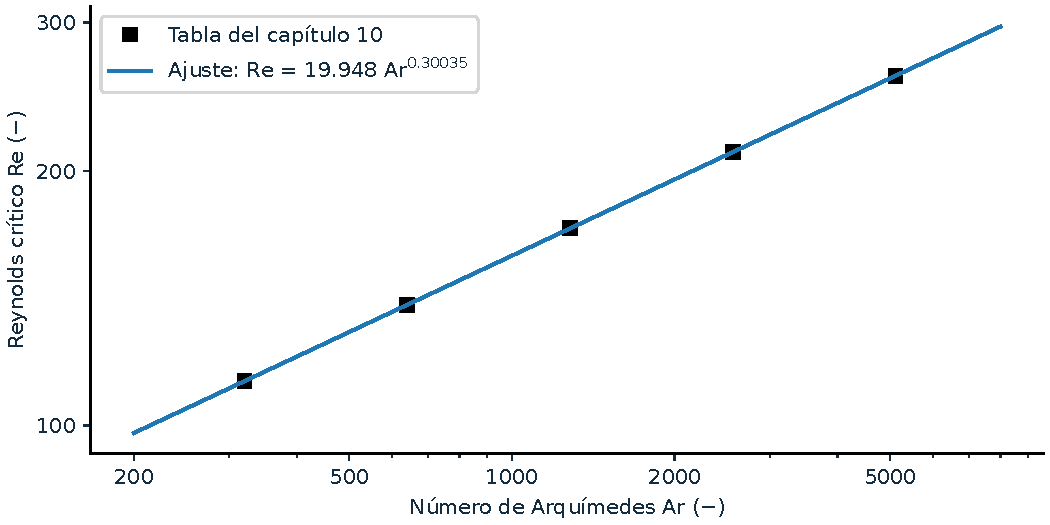
\includegraphics{../figures/FIG-0088/figure.pdf}}%
\count0=\ht0
\advance\count0 by \dp0
\count2=\wd0
\count4=\dimexpr\textheight/100*38\relax
\count6=\linewidth
\ifnum\count0<1
\count0=1
\fi
\ifnum\count2<1
\count2=1
\fi
\divide\count0 by 4096
\divide\count2 by 4096
\divide\count4 by 4096
\divide\count6 by 4096
\ifnum\count0<1
\count0=1
\fi
\ifnum\count2<1
\count2=1
\fi
\ifnum\count4<1
\count4=1
\fi
\ifnum\count6<1
\count6=1
\fi
\count8=\count2
\ifnum\count0>\count4
\count8=\numexpr\count2*\count4/\count0\relax
\fi
\ifnum\count8>\count6
\resizebox{\linewidth}{!}{\box0}%
\else
\ifnum\count0>\count4
\resizebox{!}{\dimexpr\textheight/100*38\relax}{\box0}%
\else
\box0%
\fi
\fi
\endgroup
\par\nopagebreak
\studiumcaption{fig:m06-ajuste}{Datos sintéticos del capítulo 10 en escala doble logarítmica (puntos) y correlación ajustada con FindFit, \(\mathrm{Re}_c = 19.95\,\mathrm{Ar}^{0.3003}\) (azul). Redibujada vectorialmente a partir de las ecuaciones de esta práctica; véase el registro de figuras reproducibles.}
\end{minipage}
\par\vspace{\baselineskip}

Comprobación con unidades. \texttt{Quantity} asocia unidades a cada dato y \texttt{UnitSimplify} reduce las combinaciones: si un grupo supuestamente adimensional conserva unidades, hay un error en la deducción. \texttt{DimensionalCombinations} busca automáticamente las combinaciones adimensionales de un conjunto de magnitudes; la documentación advierte que el resultado es puramente matemático y no garantiza significado físico:
\begin{lstlisting}[style=studium]
q = {Quantity[0.0648, "Meters"/"Seconds"], Quantity[4, "Millimeters"], Quantity[1, "Millipascals" "Seconds"],
     Quantity[1000, "Kilograms"/"Meters"^3], Quantity[80, "Newtons"/"Meters"^3]};
Reynolds = UnitSimplify[q[[4]] q[[1]] q[[2]]/q[[3]]];
Arq = UnitSimplify[q[[4]] q[[5]] q[[2]]^3/q[[3]]^2];
Print["B: Re = ", Reynolds, ", Ar = ", Arq, ", Ri = ", UnitSimplify[q[[5]] q[[2]]/(q[[4]] q[[1]]^2)]];
Print["B: DimensionalCombinations para Uc, d, mu, rho: ",
  DimensionalCombinations[{QuantityVariable["Uc", "Speed"], QuantityVariable["d", "Length"],
    QuantityVariable["mu", "DynamicViscosity"], QuantityVariable["rho", "MassDensity"]}]];
\end{lstlisting}
Para el ensayo a 80 N/m\(^3\) resultan \(\mathrm{Re} = 259.2\), \(\mathrm{Ar} = 5120\) y \(\mathrm{Ri} = 0.0762\), sin unidades residuales, y \texttt{DimensionalCombinations} encuentra, para \(U_c\), \(d\), \(\mu\) y \(\rho\), solo el número de Reynolds.

\section{Datos experimentales y semejanza}

Ajuste y predicción. \texttt{FindFit} ajusta el modelo \(\ln\mathrm{Re} = \ln C + n\ln\mathrm{Ar}\) a la tabla sintética del capítulo 10 y devuelve \(C = 19.95\) y \(n = 0.3003\), muy cerca de la correlación con que se generaron los datos (\(C = 20\), \(n = 0.3\)); la pequeña diferencia procede del redondeo de la tabla a 0.1 mm/s (figura~\ref{fig:m06-ajuste}):
\begin{lstlisting}[style=studium]
Bdat = {5, 10, 20, 40, 80}; Udat = {28.2, 34.7, 42.8, 52.7, 64.8} 10^-3;   (* tabla del capitulo 10 *)
dBoq = 0.004; muAgua = 1.0*^-3; rhoAgua = 1000.;
ReDat = rhoAgua Udat dBoq/muAgua; ArDat = rhoAgua Bdat dBoq^3/muAgua^2;
ajuste = FindFit[Transpose[{Log[ArDat], Log[ReDat]}], lc + n la, {lc, n}, la];
cC = Exp[lc /. ajuste]; nn = n /. ajuste;
Print["C: ajuste Re = C Ar^n con C = ", cC, ", n = ", nn];
figC = Show[ListLogLogPlot[Transpose[{ArDat, ReDat}], PlotStyle -> {Black, PointSize[0.015]}],
   LogLogPlot[cC a^nn, {a, 200, 8000}, PlotStyle -> Blue], AxesLabel -> {"Ar", "Re crit"}, ImageSize -> 380];
Export["figures/m06-ajuste.png", Rasterize[figC, Background -> White, ImageResolution -> 96]];
\end{lstlisting}
\begin{lstlisting}[style=studium]
prediccion[B_, d_, mu_, rho_] := Module[{a = rho B d^3/mu^2}, cC a^nn mu/(rho d)];
Print["D: ensayo d = 8 mm, B = 10 N/m^3: correlacion = ", 1000 prediccion[10, 0.008, muAgua, rhoAgua], " mm/s; semejanza exacta = ", 1000 0.0648 0.004/0.008, " mm/s"];
Print["D: ensayo d = 4 mm, B = 30 N/m^3: correlacion = ", 1000 prediccion[30, 0.004, muAgua, rhoAgua], " mm/s"];
Print["D: ensayo mu = 2 mPa s, d = 4 mm, B = 80 N/m^3: correlacion = ", 1000 prediccion[80, 0.004, 2.0*^-3, rhoAgua], " mm/s"];
\end{lstlisting}
Las predicciones permiten comparar los tres razonamientos del capítulo 10. Para la boquilla de 8 mm a 10 N/m\(^3\), la semejanza exacta da 32.4 mm/s y la correlación 32.42 mm/s: coinciden porque el ensayo es semejante a uno medido. Para 30 N/m\(^3\) con 4 mm, la correlación da 48.30 mm/s y la interpolación logarítmica del capítulo 48.34 mm/s: la diferencia, del orden del 0.1\,\%, cuantifica la discrepancia entre esos dos procedimientos sobre la tabla redondeada, pero \emph{no} estima por sí sola la incertidumbre experimental ni la de extrapolación del modelo. Y para la mezcla de viscosidad doble, 85.53 mm/s frente a los 85.6 mm/s de la semejanza exacta.

\begin{tcolorbox}[title={Consejo}, studiumtip, breakable]

Ajuste siempre en variables adimensionales y, para leyes de potencias, en logaritmos; ajustar \(U_c\) frente a \(\Delta(\rho g)\) directamente mezcla ensayos con distinto diámetro y no permite predecir otros. No use una correlación fuera del intervalo de números de Arquímedes en que se ajustó, y no confunda un buen ajuste con una ley física: solo describe los datos disponibles.
\end{tcolorbox}



\section{Desarrollos y práctica}

\begin{tcolorbox}[title={Ejercicios propuestos}, studiumworked, breakable]

\noindent\textbf{1 (De examen, COMPARATIVE)}
Con la correlación ajustada en la práctica 6, \(\mathrm{Re}_c = 19.948\,\mathrm{Ar}^{0.30035}\): (a) prediga la velocidad crítica del ensayo con \(d = 4.0\) mm, \(\Delta(\rho g) = 30\) N/m\(^3\), agua con \(\mu = 1.0\) mPa s y \(\rho = 1000\) kg/m\(^3\); (b) compárela con la interpolación logarítmica del capítulo 10 (48.34 mm/s) y explique a qué se debe la diferencia; (c) ¿sería fiable la correlación para \(\Delta(\rho g) = 500\) N/m\(^3\) con la misma boquilla?
\end{tcolorbox}

\begin{tcolorbox}[title={Autoevaluación}, studiumcheck, breakable]

Ejercicios propuestos. (1) Aplique \texttt{NullSpace} al problema de la resistencia de una esfera (\(F\), \(V\), \(D\), \(\rho\), \(\mu\)) y transforme la base obtenida en el coeficiente de resistencia y el número de Reynolds. (2) Escriba una función que reciba una lista de cantidades con unidades y devuelva \texttt{True} si su producto es adimensional. (3) Añada ruido aleatorio del 3 \% a la tabla, repita el ajuste veinte veces y estime la incertidumbre del exponente. (4) Diseñe un ensayo con un fluido de densidad 1200 kg/m\(^3\) que sea semejante al de 40 N/m\(^3\).
\end{tcolorbox}
\studiumchaptercheck

\chapter{Práctica 7. Navier-Stokes y métodos numéricos}
\label{chap:m07}

\studiumchapterguide{Objetivos: simplificar las ecuaciones de Navier-Stokes para un problema unidimensional no estacionario; resolverlo de forma analítica (serie de Fourier y función de error) y numérica (\texttt{NDSolve} por el método de líneas); comparar ambas soluciones; y estudiar la sensibilidad del resultado numérico a la malla y a los parámetros físicos. Se eligen problemas cuya solución exacta se conoce para poder validar el método numérico, en lugar de cálculos de fluidodinámica computacional que no se podrían comprobar.}

\section{Problemas de Navier-Stokes unidimensionales no estacionarios}

Arranque de un flujo de Couette. Entre dos placas separadas \(h = 10\) mm hay agua en reposo; en \(t = 0\) la placa inferior empieza a moverse con \(U = 0.10\) m/s. Para un flujo unidireccional \(u(y, t)\) sin gradiente de presión, la componente \(x\) de Navier-Stokes se reduce a la ecuación del calor, \(\partial u/\partial t = \nu\,\partial^{2}u/\partial y^{2}\), con las condiciones \(u(0, t) = U\), \(u(h, t) = 0\) y \(u(y, 0) = 0\). Por separación de variables, la solución es la del estado estacionario, el perfil lineal de Couette, menos una serie de modos que se amortiguan exponencialmente:
\begin{equation}
u(y,t) = U\left(1 - \frac{y}{h}\right) - \frac{2U}{\pi}\sum_{n=1}^{\infty}\frac{1}{n}\,e^{-n^{2}\pi^{2}\nu t/h^{2}}\sin\frac{n\pi y}{h}. \label{eq:m07-serie}
\end{equation}
El tiempo característico es el tiempo viscoso \(h^{2}/\nu = (0.010)^2/1.0\times 10^{-6} = 100\) s. El primer bloque programa la serie (truncada, y protegida frente a exponenciales que el ordenador no puede representar) y comprueba simbólicamente que cumple la ecuación:
\begin{lstlisting}[style=studium]
ClearAll["Global`*"];
nu = 1.0*^-6; h = 0.010; U = 0.10;          (* agua, holgura de 10 mm, placa inferior a 0,1 m/s *)
(* u_t = nu u_yy,  u(0,t) = U (placa movil), u(h,t) = 0 (placa fija), u(y,0) = 0 *)
serie[y_, t_, nmax_: 40] := U (1 - y/h) - (2 U/Pi) Sum[If[n^2 Pi^2 nu t/h^2 < 700, Exp[-n^2 Pi^2 nu t/h^2], 0] Sin[n Pi y/h]/n, {n, 1, nmax}];
Print["A: tiempo viscoso h^2/nu = ", h^2/nu, " s"];
serieSim[y_, t_] := U (1 - y/h) - (2 U/Pi) Sum[Exp[-n^2 Pi^2 nu t/h^2] Sin[n Pi y/h]/n, {n, 1, 20}];
Print["A: comprobacion de la serie (20 terminos): residuo de la EDP en (h/3, 10 s) = ",
  (D[serieSim[y, t], t] - nu D[serieSim[y, t], {y, 2}]) /. {y -> h/3, t -> 10.}];
\end{lstlisting}

\par\vspace{\baselineskip}
\noindent\begin{minipage}{\linewidth}
\centering
\begingroup
\setbox0=\hbox{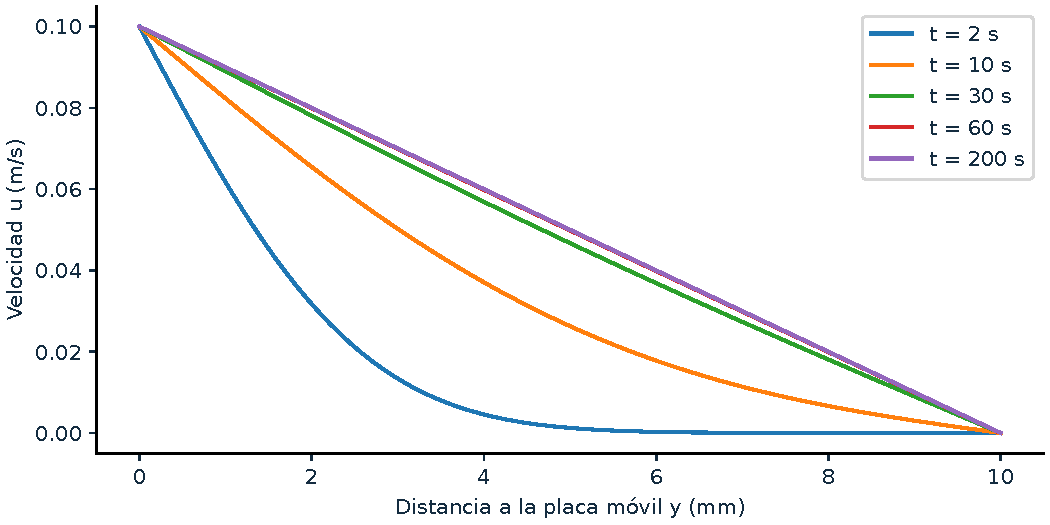
\includegraphics{../figures/FIG-0089/figure.pdf}}%
\count0=\ht0
\advance\count0 by \dp0
\count2=\wd0
\count4=\dimexpr\textheight/100*38\relax
\count6=\linewidth
\ifnum\count0<1
\count0=1
\fi
\ifnum\count2<1
\count2=1
\fi
\divide\count0 by 4096
\divide\count2 by 4096
\divide\count4 by 4096
\divide\count6 by 4096
\ifnum\count0<1
\count0=1
\fi
\ifnum\count2<1
\count2=1
\fi
\ifnum\count4<1
\count4=1
\fi
\ifnum\count6<1
\count6=1
\fi
\count8=\count2
\ifnum\count0>\count4
\count8=\numexpr\count2*\count4/\count0\relax
\fi
\ifnum\count8>\count6
\resizebox{\linewidth}{!}{\box0}%
\else
\ifnum\count0>\count4
\resizebox{!}{\dimexpr\textheight/100*38\relax}{\box0}%
\else
\box0%
\fi
\fi
\endgroup
\par\nopagebreak
\studiumcaption{fig:m07-arranque}{Arranque de un flujo de Couette en agua (\(h = 10\) mm, \(U = 0.10\) m/s): perfiles de velocidad calculados con la serie de Fourier de 160 términos a 2, 10, 30, 60 y 200 s. Redibujada vectorialmente a partir de las ecuaciones de esta práctica; véase el registro de figuras reproducibles.}
\end{minipage}
\par\vspace{\baselineskip}

Solución numérica. \texttt{NDSolveValue} resuelve la ecuación en derivadas parciales por el método de líneas: discretiza \(y\) en una malla y convierte la ecuación en un sistema de ecuaciones diferenciales ordinarias en \(t\). La condición inicial es discontinua en \(y = 0\) (el fluido está en reposo, pero la placa ya se mueve), y se expresa con \texttt{If}. El número de puntos de la malla se controla con la opción \texttt{SpatialDiscretization}:
\begin{lstlisting}[style=studium]
resolver[pts_] := NDSolveValue[{D[u[y, t], t] == nu D[u[y, t], {y, 2}], u[0, t] == U, u[h, t] == 0,
     u[y, 0] == If[y == 0, U, 0]}, u, {y, 0, h}, {t, 0, 200},
   Method -> {"MethodOfLines", "SpatialDiscretization" -> {"TensorProductGrid", "MinPoints" -> pts, "MaxPoints" -> pts}}];
sol = resolver[101];
errores = Table[Abs[sol[yy, tt] - serie[yy, tt]], {tt, {5., 20., 60.}}, {yy, h/10, 9 h/10, h/10}];
Print["B: error maximo frente a la serie en t = 5, 20, 60 s: ", Max /@ errores, " m/s"];
figB = Plot[Evaluate[Table[sol[y, tt], {tt, {2, 10, 30, 60, 200}}]], {y, 0, h},
   PlotLegends -> {"t = 2 s", "10 s", "30 s", "60 s", "200 s"}, AxesLabel -> {"y (m)", "u (m/s)"}, ImageSize -> 400];
Export["figures/m07-arranque.png", Rasterize[figB, Background -> White, ImageResolution -> 96]];
\end{lstlisting}
Con 101 puntos, la diferencia máxima entre la solución numérica y la serie es \(3\times 10^{-5}\) m/s, un 0.03 \% de \(U\), en los instantes 5, 20 y 60 s. La figura~\ref{fig:m07-arranque} muestra cómo la cantidad de movimiento se difunde desde la placa móvil: a los 2 s solo se mueve apreciablemente una capa de unos 5 mm; a los 60 s el perfil es prácticamente el lineal.

\section{Comprobación y sensibilidad de las soluciones numéricas}

Esfuerzo en la placa fija y condicionamiento. El esfuerzo que el fluido transmite a la placa fija crece desde cero hasta el valor estacionario \(\mu U/h = 0.01\) Pa. A 10, 30 y 60 s la solución numérica da el 29.40 \%, el 89.53 \% y el 99.35 \% de ese valor, frente al 29.29 \%, el 89.65 \% y el 99.46 \% de la serie: el esfuerzo, que es una derivada, tiene un error del orden del 0.1 \%, mayor que el de la velocidad. El instante en que el esfuerzo alcanza el 99 \% es 53.68 s según la serie analítica y se comunica como 55.1 s para la simulación indicada. La diferencia no demuestra por sí misma que la solución numérica sea correcta: al tiempo de 55.1 s, la serie predice aproximadamente el 99.1305 \% del esfuerzo estacionario; bastaría un sesgo numérico de unas 0.1305 unidades porcentuales de ese esfuerzo para desplazar así el cruce. El cálculo debe reproducirse y contrastarse refinando el método de derivación espacial y las tolerancias temporales:
\begin{lstlisting}[style=studium]
tauFija[t_?NumericQ] := -(10^-3) Derivative[1, 0][sol][h, t];      (* mu = 10^-3 Pa s *)
tauEst = 10^-3 U/h;
razonSerie[t_?NumericQ] := 1 + 2 Sum[(-1)^n If[n^2 Pi^2 nu t/h^2 < 700, Exp[-n^2 Pi^2 nu t/h^2], 0], {n, 1, 40}];
Print["C: tau/tau_est en t = 10, 30, 60 s, NDSolve: ", Table[tauFija[tt]/tauEst, {tt, {10., 30., 60.}}], " ; serie: ", Table[razonSerie[tt], {tt, {10., 30., 60.}}]];
t99 = t /. FindRoot[tauFija[t] == 0.99 tauEst, {t, 60}];
t99an = t /. FindRoot[razonSerie[t] == 0.99, {t, 40, 70}, Method -> "Brent"];
Print["C: t para el 99 % del esfuerzo: NDSolve = ", t99, " s, serie = ", t99an, " s = ", t99an nu/h^2, " h^2/nu"];
(* Un error del 0,1 % en el esfuerzo desplaza el instante del 99 % en mas de un segundo: cerca de una
   asintota, un tiempo de cruce es una magnitud mal condicionada. *)
\end{lstlisting}
La lección práctica es elegir magnitudes bien condicionadas para comparar soluciones (valores en instantes fijos, no tiempos de cruce) y comprobar las derivadas con más cuidado que las funciones.

Sensibilidad a la malla y a los parámetros. Con 11, 21, 51 y 101 puntos la velocidad en el centro a los 20 s es 0,041191, 0,041139, 0.041137 y 0.041138 m/s, frente a 0.041157 m/s de la serie: entre 21 y 101 puntos el resultado cambia poco; sin embargo, la diferencia residual con la serie (aproximadamente un 0.05 \% de la velocidad) no permite atribuir el error exclusivamente a la discontinuidad inicial o a las tolerancias temporales. Para distinguir esas causas hay que refinar de manera independiente la discretización espacial y los objetivos de precisión temporal. Con 11 puntos Mathematica avisa de que no puede estimar el error espacial: un aviso que no debe ignorarse. Cambiar la viscosidad sí cambia el resultado de forma importante (0,0263, 0.0411 y 0.0487 m/s para \(\nu/2\), \(\nu\) y \(2\nu\)), porque el tiempo físico relevante es \(h^{2}/\nu\):
\begin{lstlisting}[style=studium]
Print["D: u(h/2, 20 s) con 11, 21, 51 y 101 puntos: ", Table[resolver[n][h/2, 20.], {n, {11, 21, 51, 101}}], " ; serie: ", serie[h/2, 20.]];
Print["D: u(h/2, 20 s) con nu x 0.5, 1, 2: ", Table[Block[{nu = f 1.0*^-6}, resolver[51][h/2, 20.]], {f, {0.5, 1, 2}}]];
\end{lstlisting}
Primer problema de Stokes. Si la placa móvil está sola frente a un fluido semi-infinito, la solución es \(u = U\,\mathrm{erfc}\!\left(y/(2\sqrt{\nu t})\right)\) y la capa afectada crece como \(\sqrt{\nu t}\); el bloque E comprueba que la velocidad cae al 1 \% de \(U\) a \(3.64\sqrt{\nu t}\), 36.4 mm a los 100 s, porque \(3.64\cdot\sqrt{1.0\times 10^{-6}\cdot 100} = 0.0364\) m, y que \texttt{NDSolve} en un dominio de 50 mm reproduce la solución con un error de \(2\times 10^{-5}\) m/s:
\begin{lstlisting}[style=studium]
stokes[y_, t_] := U Erfc[y/(2 Sqrt[nu t])];
solS = NDSolveValue[{D[w[y, t], t] == nu D[w[y, t], {y, 2}], w[0, t] == U, w[0.05, t] == 0, w[y, 0] == If[y == 0, U, 0]},
   w, {y, 0, 0.05}, {t, 0, 100}];
Print["E: espesor 1 % (y donde u = 0.01 U) en t = 100 s: ", y /. FindRoot[stokes[y, 100.] == 0.01 U, {y, 0.02}], " m; 3.64 sqrt(nu t) = ", 3.64 Sqrt[nu 100.]];
Print["E: error maximo NDSolve frente a erfc en t = 100 s: ", Max[Table[Abs[solS[yy, 100.] - stokes[yy, 100.]], {yy, 0, 0.03, 0.001}]], " m/s"];
\end{lstlisting}

\begin{tcolorbox}[title={Consejo}, studiumtip, breakable]

Antes de confiar en una solución numérica de una ecuación en derivadas parciales: compruebe que hay tantas condiciones de contorno e iniciales como exige la ecuación; resuelva primero un caso con solución exacta; refine la malla hasta que el resultado deje de cambiar; no ignore los avisos de \texttt{NDSolve}; y prefiera comparar magnitudes bien condicionadas. En un dominio que representa un medio infinito, compruebe que el borde está lo bastante lejos (varias veces \(\sqrt{\nu t}\)).
\end{tcolorbox}



\section{Desarrollos y práctica}

\begin{tcolorbox}[title={Desarrollos del modelo}, studiumdef, breakable]

\noindent\textbf{Arranque de un flujo de Couette: solución en serie de Fourier}

\begin{equation}
\frac{\partial u}{\partial t} = \nu\,\frac{\partial^{2}u}{\partial y^{2}},\qquad u(y,t) = U\left(1 - \frac{y}{h}\right) - \frac{2U}{\pi}\sum_{n=1}^{\infty}\frac{1}{n}\,e^{-n^{2}\pi^{2}\nu t/h^{2}}\sin\frac{n\pi y}{h}
\label{eq:m07-arranque}
\end{equation}

\noindent\textbf{Hipótesis}
\begin{itemize}
\item flujo unidireccional u(y,t) entre placas indefinidas
\item sin gradiente de presión
\item placa en y = 0 que arranca bruscamente con velocidad U; placa en y = h fija
\item fluido en reposo en t = 0
\end{itemize}

\noindent\textbf{Principios}
\begin{itemize}
\item componente x de Navier-Stokes para un flujo unidireccional
\item separación de variables
\end{itemize}

\noindent\textbf{Condiciones de contorno}
\begin{itemize}
\item u(0, t) = U
\item u(h, t) = 0
\item u(y, 0) = 0 para 0 < y < h
\end{itemize}

\noindent\textbf{Limitaciones}
\begin{itemize}
\item la serie converge lentamente en t muy pequeño; allí es mejor la solución de Stokes con erfc
\end{itemize}

\noindent\textbf{Pasos}
\begin{enumerate}
\item
Navier-Stokes se reduce a la ecuación del calor

\[
\frac{\partial u}{\partial t} = \nu\,\frac{\partial^{2}u}{\partial y^{2}}
\]
\item
solución estacionaria

\[
u_s = U\left(1 - \frac{y}{h}\right)
\]
\item
parte transitoria con condiciones homogéneas

\[
u - u_s = \sum_{n} b_n\,e^{-n^{2}\pi^{2}\nu t/h^{2}}\sin\frac{n\pi y}{h}
\]
\item
coeficientes de Fourier de la condición inicial

\[
b_n = -\frac{2U}{n\pi}
\]
\end{enumerate}

\noindent\textbf{Variables}
\begin{itemize}
\item $\nu$: viscosidad cinemática ($\mathrm{m}^{2}\,\mathrm{s}^{-1}$)
\item $h$: separación entre placas ($\mathrm{m}$)
\end{itemize}


\end{tcolorbox}

\begin{tcolorbox}[title={Problema resuelto}, studiumworked, breakable]

\noindent\textbf{Enunciado}

En el arranque de Couette entre dos placas separadas una distancia \(h=10\,\mathrm{mm}\), con viscosidad cinemática \(\nu=1.0\times10^{-6}\,\mathrm{m^2/s}\), calcule el tiempo viscoso característico de difusión de cantidad de movimiento a través de la separación.

\noindent\textbf{Desarrollo paso a paso}

\noindent\textbf{Elección del procedimiento.} En $\partial_tu=\nu\partial_{yy}u$, las escalas son $U/t_\nu$ y $\nu U/h^2$. Igualarlas cancela la velocidad característica y da $t_\nu=h^2/\nu$. Es una escala; el criterio de estacionariedad necesita además una tolerancia.

\begin{enumerate}

\item Convertir primero 10 mm en 0,010 m; el cuadrado convierte el factor mil en un millón.

\[\fitmath{\mathrm{tnu}=\frac{{h}^{2}}{\nu}}\]

\[\fitmath{\mathrm{tnu}=\frac{{(0{,}01)}^{2}}{(1\times10^{-6})}\approx 100\,\mathrm{s}}\]

\end{enumerate}


\noindent\textbf{Respuesta}

\(t_{\nu}=100\,\mathrm{s}\)
\end{tcolorbox}

\begin{tcolorbox}[title={Ejercicios propuestos}, studiumworked, breakable]

\noindent\textbf{1 (Avanzado, Desarrollo)}
En el arranque del flujo de Couette de la práctica 7 (\(h = 10\) mm, \(\nu = 1.0\times 10^{-6}\) m\(^2\)/s), el esfuerzo en la placa fija vale, según la serie, \(\tau/\tau_{\mathrm{est}} = 1 + 2\sum_{n\ge 1}(-1)^{n}e^{-n^{2}\pi^{2}\nu t/h^{2}}\). (a) Justifique que para \(t\) del orden de \(h^{2}/\nu\) basta el primer término. (b) Obtenga con él el instante en que el esfuerzo alcanza el 99 \% del estacionario. (c) Explique por qué la solución numérica da 55.1 s.
\end{tcolorbox}

\begin{tcolorbox}[title={Autoevaluación}, studiumcheck, breakable]

Ejercicios propuestos. (1) Resuelva el arranque de un flujo de Poiseuille plano, \(\partial u/\partial t = G/\rho + \nu\,\partial^{2}u/\partial y^{2}\) con las dos placas fijas, y compare el tiempo de establecimiento con el del flujo de Couette. (2) Segundo problema de Stokes: haga oscilar la placa, \(u(0, t) = U\cos\omega t\), y mida la profundidad de penetración frente a \(\sqrt{2\nu/\omega}\). (3) Repita la práctica con un aceite cuya viscosidad cinemática sea del orden de \(10^{-4}\) m\(^2\)/s y explique el cambio de escala de tiempos. (4) Estudie cómo cambia el error del esfuerzo en la placa fija al usar diferencias finitas de cuarto orden.
\end{tcolorbox}
\studiumchaptercheck

\appendix
\chapter{Notación y unidades}

\begingroup
\setlength{\LTpre}{0pt}
\setlength{\LTpost}{0pt}
\begin{longtable}{@{}>{\centering\arraybackslash}p{0.17\linewidth}>{\raggedright\arraybackslash}p{0.55\linewidth}>{\raggedright\arraybackslash}p{0.2\linewidth}@{}}
\textbf{Símbolo} & \textbf{Significado} & \textbf{Unidades} \\
\hline
\endfirsthead
\textbf{Símbolo} & \textbf{Significado} & \textbf{Unidades} \\
\hline
\endhead
$A_{e}$ & área de la sección de salida de la tobera & $\mathrm{m^{2}}$ \\
$C_{D}$ & coeficiente de resistencia &  \\
$C_{L}$ & coeficiente de sustentación &  \\
$C_{P}$ & coeficiente de potencia de una turbina &  \\
$C_{T}$ & coeficiente de empuje de una hélice &  \\
$C_{p}$ & coeficiente de presión &  \\
$C_{D0}$ & coeficiente de resistencia parásita (a sustentación nula) &  \\
$D$ & diámetro de un conducto & $\mathrm{m}$ \\
$D_{h}$ & diámetro hidráulico, 4A/P & $\mathrm{m}$ \\
$D_{m}$ & coeficiente de difusión másica & $\mathrm{m^{2}\,s^{-1}}$ \\
$E_{c}$ & energía cinética & $\mathrm{J}$ \\
$E_{p}$ & energía potencial & $\mathrm{J}$ \\
$F$ & empuje de un sistema propulsor & $\mathrm{N}$ \\
$F_{t}$ & fuerza de tracción que la calzada ejerce sobre las ruedas motrices & $\mathrm{N}$ \\
$G$ & gradiente de presión motor, G = -dp/dx & $\mathrm{Pa\,m^{-1}}$ \\
$H_{e}$ & altura de escala de una atmósfera isoterma & $\mathrm{m}$ \\
$i$ & momento de inercia respecto a un eje & $\mathrm{kg m^{2}}$ \\
$I_{sp}$ & impulso específico & $\mathrm{s}$ \\
$I_{xc}$ & momento de inercia de área respecto al eje horizontal que pasa por el centroide & $\mathrm{m^{4}}$ \\
$J$ & grado de avance de una hélice &  \\
$K$ & coeficiente cuadrático total de la polar de la polar parabólica &  \\
$L'$ & sustentación por unidad de envergadura & $\mathrm{N\,m^{-1}}$ \\
$M$ & masa total de un sistema de partículas & $\mathrm{kg}$ \\
$N$ & frecuencia de Brunt-Väisälä & $\mathrm{1\,s^{-1}}$ \\
$Q$ & caudal volumétrico & $\mathrm{m^{3}\,s^{-1}}$ \\
$Q_{f}$ & factor de calidad de un oscilador &  \\
$R_{a}$ & constante específica del aire seco & $\mathrm{J\,(kg K)^{-1}}$ \\
$S$ & superficie de referencia (alar en aviones) & $\mathrm{m^{2}}$ \\
$T$ & temperatura absoluta & $\mathrm{K}$ \\
$T'$ & par por unidad de longitud de cilindro & $\mathrm{N m\,m^{-1}}$ \\
$U_{c}$ & velocidad crítica de inicio de la inestabilidad de un chorro & $\mathrm{m\,s^{-1}}$ \\
$V$ & velocidad media en una sección & $\mathrm{m\,s^{-1}}$ \\
$V_\infty$ & velocidad de la corriente libre & $\mathrm{m\,s^{-1}}$ \\
$V_{t}$ & velocidad terminal & $\mathrm{m\,s^{-1}}$ \\
$W$ & trabajo de una fuerza & $\mathrm{J}$ \\
$\Delta(\rho g)$ & flotabilidad por unidad de volumen (diferencia de peso específico) & $\mathrm{N\,m^{-3}}$ \\
$\Gamma$ & gradiente vertical de temperatura de la atmósfera (positivo si T disminuye con la altura) & $\mathrm{K\,m^{-1}}$ \\
$\Gamma_C$ & circulación de la velocidad a lo largo de la curva cerrada C & $\mathrm{m^{2}\,s^{-1}}$ \\
$\Omega_1, \Omega_2$ & velocidades angulares de los cilindros interior y exterior & $\mathrm{rad\,s^{-1}}$ \\
$\Phi$ & función de disipación viscosa (potencia disipada por unidad de volumen) & $\mathrm{W\,m^{-3}}$ \\
$\Phi_v$ & función de disipación viscosa & $\mathrm{W\,m^{-3}}$ \\
$\Pi_i$ & grupo adimensional i-ésimo del teorema Pi &  \\
$\alpha$ & ángulo de ataque & $\mathrm{rad}$ \\
$\alpha_T$ & difusividad térmica & $\mathrm{m^{2}\,s^{-1}}$ \\
$\beta$ & propiedad intensiva por unidad de masa en el teorema del transporte &  \\
$\beta_T$ & coeficiente de dilatación térmica & $\mathrm{1\,K^{-1}}$ \\
$\boldsymbol{\Omega}$ & velocidad angular de un sólido o de un sistema de referencia & $\mathrm{rad\,s^{-1}}$ \\
$\boldsymbol{\omega}$ & vorticidad, rotacional de la velocidad & $\mathrm{1\,s^{-1}}$ \\
$\boldsymbol{\sigma}$ & tensor de esfuerzos de Cauchy & $\mathrm{Pa}$ \\
$\boldsymbol{\tau}$ & tensor de esfuerzos viscosos & $\mathrm{Pa}$ \\
$\boldsymbol{\xi}$ & etiqueta lagrangiana: posición de una partícula en el instante inicial & $\mathrm{m}$ \\
$\delta$ & decremento logarítmico &  \\
$\delta_{cl}$ & espesor de la capa límite & $\mathrm{m}$ \\
$\dot W'$ & potencia por unidad de longitud de cilindro & $\mathrm{W\,m^{-1}}$ \\
$\dot m$ & gasto másico & $\mathrm{kg\,s^{-1}}$ \\
$\epsilon_h$ & cociente de aspecto de una capa delgada, h/L &  \\
$\eta_p$ & rendimiento propulsivo &  \\
$\frac{D}{Dt}$ & derivada material (siguiendo a la partícula) & $\mathrm{1\,s^{-1}}$ \\
$\kappa$ & conductividad térmica & $\mathrm{W\,(m K)^{-1}}$ \\
$\lambda$ & recorrido libre medio molecular & $\mathrm{m}$ \\
$\lambda_v$ & segundo coeficiente de viscosidad & $\mathrm{Pa s}$ \\
$\mathbf{A}_v$ & potencial vector & $\mathrm{m^{2}\,s^{-1}}$ \\
$\mathbf{E}$ & tensor de velocidad de deformación (parte simétrica del gradiente de velocidad) & $\mathrm{1\,s^{-1}}$ \\
$\mathbf{F}$ & fuerza & $\mathrm{N}$ \\
$\mathbf{I}$ & tensor identidad &  \\
$\mathbf{L}_O$ & momento angular respecto al punto O & $\mathrm{kg m^{2}\,s^{-1}}$ \\
$\mathbf{M}_O$ & momento resultante de las fuerzas respecto al punto O & $\mathrm{N m}$ \\
$\mathbf{P}$ & momento lineal total de un sistema & $\mathrm{kg m\,s^{-1}}$ \\
$\mathbf{R}_G$ & posición del centro de masas & $\mathrm{m}$ \\
$\mathbf{W}$ & tensor de rotación (parte antisimétrica del gradiente de velocidad) & $\mathrm{1\,s^{-1}}$ \\
$\mathbf{a}$ & aceleración de una partícula & $\mathrm{m\,s^{-2}}$ \\
$\mathbf{a}_0$ & aceleración del origen de un sistema de referencia no inercial & $\mathrm{m\,s^{-2}}$ \\
$\mathbf{f}$ & fuerza neta por unidad de volumen sobre un elemento fluido & $\mathrm{N\,m^{-3}}$ \\
$\mathbf{f}_m$ & fuerza de volumen por unidad de masa & $\mathrm{m\,s^{-2}}$ \\
$\mathbf{g}$ & aceleración de la gravedad (vector) & $\mathrm{m\,s^{-2}}$ \\
$\mathbf{n}$ & vector unitario normal exterior &  \\
$\mathbf{p}$ & momento lineal de una partícula & $\mathrm{kg m\,s^{-1}}$ \\
$\mathbf{r}$ & vector de posición & $\mathrm{m}$ \\
$\mathbf{r}'$ & posición medida en el sistema de referencia móvil & $\mathrm{m}$ \\
$\mathbf{t}$ & vector tensión (fuerza de superficie por unidad de área) & $\mathrm{Pa}$ \\
$\mathbf{u}$ & velocidad del fluido (campo euleriano) & $\mathrm{m\,s^{-1}}$ \\
$\mathbf{v}$ & velocidad de una partícula & $\mathrm{m\,s^{-1}}$ \\
$\mathbf{v}'$ & velocidad relativa al sistema de referencia móvil & $\mathrm{m\,s^{-1}}$ \\
$\mathbf{x}$ & posición de un punto del espacio & $\mathrm{m}$ \\
$\mathcal{A}$ & alargamiento del ala, $b^{2}/S$ & adimensional \\
$\mathcal{L}$ & lagrangiana de un sistema mecánico & $\mathrm{J}$ \\
$\mathrm{Ar}$ & número de Arquímedes, $\rho\,\Delta\rho\,g\,d^{3}/\mu^{2}$ & adimensional \\
$\mathrm{Eu}$ & número de Euler &  \\
$\mathrm{Fr}$ & número de Froude &  \\
$\mathrm{Gr}$ & número de Grashof, $g\beta\,\Delta T\,L^{3}/\nu^{2}$ & adimensional \\
$\mathrm{Kn}$ & número de Knudsen &  \\
$\mathrm{Ma}$ & número de Mach &  \\
$\mathrm{Pr}$ & número de Prandtl &  \\
$\mathrm{Re}$ & número de Reynolds &  \\
$\mathrm{Ri}$ & número de Richardson densimétrico, $(\Delta\rho\,g\,d)/(\rho U^{2})$ & adimensional \\
$\mathrm{Ro}$ & número de Rossby &  \\
$\mathrm{St}$ & número de Strouhal &  \\
$\mathrm{Wo}$ & número de Womersley &  \\
$\mu$ & viscosidad dinámica & $\mathrm{Pa s}$ \\
$\nabla$ & operador nabla & $\mathrm{1\,m^{-1}}$ \\
$\nabla^{2}$ & operador laplaciano & $\mathrm{1\,m^{-2}}$ \\
$\nu$ & viscosidad cinemática & $\mathrm{m^{2}\,s^{-1}}$ \\
$\omega_0$ & pulsación natural no amortiguada & $\mathrm{rad\,s^{-1}}$ \\
$\omega_d$ & pulsación natural amortiguada & $\mathrm{rad\,s^{-1}}$ \\
$\phi$ & potencial de velocidad & $\mathrm{m^{2}\,s^{-1}}$ \\
$\psi$ & función de corriente & $\mathrm{m^{2}\,s^{-1}}$ \\
$\rho$ & densidad & $\mathrm{kg\,m^{-3}}$ \\
$\rho'$ & perturbación de densidad respecto al valor de referencia & $\mathrm{kg\,m^{-3}}$ \\
$\tau$ & esfuerzo cortante & $\mathrm{Pa}$ \\
$\tau_w$ & esfuerzo cortante en la pared & $\mathrm{Pa}$ \\
$\tau_{r\theta}$ & esfuerzo cortante en la dirección azimutal sobre una superficie r = cte & $\mathrm{Pa}$ \\
$\varepsilon$ & rugosidad absoluta de la pared de un conducto & $\mathrm{m}$ \\
$\varphi$ & ángulo de una pendiente con la horizontal & $\mathrm{rad}$ \\
$\zeta$ & factor de amortiguamiento &  \\
$a$ & factor de inducción axial del disco actuador &  \\
$a_{s}$ & velocidad del sonido & $\mathrm{m\,s^{-1}}$ \\
$c$ & coeficiente de amortiguamiento viscoso & $\mathrm{N s\,m^{-1}}$ \\
$d$ & diámetro de una partícula o esfera & $\mathrm{m}$ \\
$e$ & factor de eficiencia de Oswald &  \\
$f$ & parámetro de Coriolis & $\mathrm{1\,s^{-1}}$ \\
$f_{D}$ & factor de fricción de Darcy &  \\
$f_{s}$ & frecuencia de desprendimiento de torbellinos & $\mathrm{Hz}$ \\
$g$ & aceleración de la gravedad & $\mathrm{m\,s^{-2}}$ \\
$g'$ & gravedad reducida & $\mathrm{m\,s^{-2}}$ \\
$h$ & profundidad bajo una superficie libre & $\mathrm{m}$ \\
$h_{c}$ & profundidad del centroide de una superficie sumergida & $\mathrm{m}$ \\
$h_{f}$ & espesor de una película o capa delgada & $\mathrm{m}$ \\
$h_{cp}$ & profundidad del centro de presiones & $\mathrm{m}$ \\
$k$ & rigidez de un muelle o constante recuperadora & $\mathrm{N\,m^{-1}}$ \\
$k_{B}$ & constante de Boltzmann & $\mathrm{J\,K^{-1}}$ \\
$k_{D}$ & constante de resistencia aerodinámica cuadrática, $k_D = \tfrac{1}{2}\rho C_D A$ & $\mathrm{kg\,m^{-1}}$ \\
$k_{w}$ & número de onda & $\mathrm{1\,m^{-1}}$ \\
$m$ & masa de una partícula o de un cuerpo & $\mathrm{kg}$ \\
$n_{v}$ & número de moléculas por unidad de volumen & $\mathrm{1\,m^{-3}}$ \\
$p$ & presión & $\mathrm{Pa}$ \\
$p_{0}$ & presión de referencia (en la superficie libre o a nivel del mar) & $\mathrm{Pa}$ \\
$p_{e}$ & presión en la sección de salida de la tobera & $\mathrm{Pa}$ \\
$p_{t}$ & presión de remanso o total & $\mathrm{Pa}$ \\
$p_{atm}$ & presión atmosférica local & $\mathrm{Pa}$ \\
$q$ & caudal por unidad de anchura entre placas & $\mathrm{m^{2}\,s^{-1}}$ \\
$q_\infty$ & presión dinámica de la corriente libre, $\tfrac{1}{2}\rho V^{2}$ & $\mathrm{Pa}$ \\
$q_{j}$ & coordenada generalizada j-ésima &  \\
$t$ & tiempo & $\mathrm{s}$ \\
$\left( u, \  v, \  w\right)$ & componentes cartesianas de la velocidad del fluido & $\mathrm{m\,s^{-1}}$ \\
$u_\theta$ & componente azimutal de la velocidad en coordenadas cilíndricas & $\mathrm{m\,s^{-1}}$ \\
$\left( u_{g}, \  v_{g}\right)$ & componentes del viento geostrófico & $\mathrm{m\,s^{-1}}$ \\
$v_{0}$ & velocidad de vuelo (velocidad de la corriente libre respecto al motor) & $\mathrm{m\,s^{-1}}$ \\
$v_{e}$ & velocidad de salida del chorro respecto al motor & $\mathrm{m\,s^{-1}}$ \\
$v_{i}$ & velocidad inducida en el disco de un rotor & $\mathrm{m\,s^{-1}}$ \\
$x_{n}$ & iterado n-ésimo del mapa logístico &  \\
$z$ & coordenada vertical, positiva hacia arriba & $\mathrm{m}$ \\
\end{longtable}
\endgroup
\chapter{Formulario y condiciones de uso}

\noindent\textbf{Teorema del centro de masas}

\[
M\,\frac{d^{2}\mathbf{R}_G}{dt^{2}} = \sum_i \mathbf{F}_i^{\mathrm{ext}}
\]

\noindent\textbf{Ecuación del momento angular de una partícula}

\[
\frac{d\mathbf{L}_O}{dt} = \mathbf{r}\times\mathbf{F} = \mathbf{M}_O
\]

\noindent\textbf{Teorema del trabajo y la energía cinética}

\[
W_{12} = \int_{1}^{2}\mathbf{F}\cdot d\mathbf{r} = \tfrac{1}{2}m v_2^{2} - \tfrac{1}{2}m v_1^{2}
\]

\noindent\textbf{Conservación de la energía mecánica en un campo gravitatorio uniforme}

\[
\tfrac{1}{2}m v_2^{2} + m g z_2 = \tfrac{1}{2}m v_1^{2} + m g z_1
\]

\noindent\textbf{Aceleración vista desde un sistema de referencia giratorio}

\[
\mathbf{a} = \mathbf{a}' + 2\boldsymbol{\Omega}\times\mathbf{v}' + \boldsymbol{\Omega}\times\left(\boldsymbol{\Omega}\times\mathbf{r}'\right) + \dot{\boldsymbol{\Omega}}\times\mathbf{r}'
\]

\noindent\textbf{Ecuación del péndulo simple a partir de la lagrangiana}

\[
\ddot{\theta} + \frac{g}{\ell}\sin\theta = 0
\]

\noindent\textbf{Punto fijo no trivial del mapa logístico}

\[
x^{*} = 1 - \frac{1}{r},\qquad \left|f'(x^{*})\right| = |2 - r| < 1 \iff 1 < r < 3
\]

\noindent\textbf{Densidad de un gas ideal}

\[
\rho = \frac{p}{R_a T}
\]

\noindent\textbf{Densidad numérica de un gas ideal}

\[
n_v = \frac{p}{k_B T}
\]

\noindent\textbf{Esfuerzo cortante en una película de perfil lineal}

\[
\tau = \mu\,\frac{U}{h}
\]

\noindent\textbf{Par y potencia viscosos en un cojinete de holgura delgada}

\[
M = \frac{2\pi\mu\,\omega R^{3} L}{c},\qquad \dot W = M\omega = \frac{2\pi\mu\,\omega^{2} R^{3} L}{c}
\]

\noindent\textbf{Aceleración material en una tobera unidimensional}

\[
a = \frac{Du}{Dt} = \frac{\partial u}{\partial t} + u\,\frac{\partial u}{\partial x} = \frac{U_0^{2}}{L}\left(1 + \frac{x}{L}\right)
\]

\noindent\textbf{Trayectorias del flujo plano de punto de remanso}

\[
x\,y = x_0\,y_0
\]

\noindent\textbf{Traza de un flujo uniforme con componente transversal creciente}

\[
y = \frac{a}{2}\left(\frac{2 t x}{u_0} - \frac{x^{2}}{u_0^{2}}\right)
\]

\noindent\textbf{Ecuación fundamental de la hidrostática}

\[
p = p_0 + \rho g h
\]

\noindent\textbf{Superficie libre de un líquido en rotación como sólido rígido}

\[
z_s(r) = z_0 + \frac{\Omega^{2} r^{2}}{2g}
\]

\noindent\textbf{Fuerza y centro de presiones sobre una superficie plana vertical rectangular}

\[
F = \rho g\,h_c\,A,\qquad h_{cp} = h_c + \frac{I_{xc}}{h_c A}
\]

\noindent\textbf{Presión en una atmósfera isoterma}

\[
p = p_0\,\exp\!\left(-\frac{g z}{R_a T}\right) = p_0\,e^{-z/H_e},\qquad H_e = \frac{R_a T}{g}
\]

\noindent\textbf{Presión en una troposfera con gradiente térmico constante}

\[
T = T_0 - \Gamma z,\qquad p = p_0\left(1 - \frac{\Gamma z}{T_0}\right)^{g/(R_a\Gamma)}
\]

\noindent\textbf{Flujo de Couette con gradiente de presión}

\[
u(y) = \frac{G}{2\mu}\,y\,(h - y) + U\,\frac{y}{h},\qquad G = -\frac{dp}{dx}
\]

\noindent\textbf{Caudal del flujo de Poiseuille plano}

\[
q = \int_0^{h} u\,dy = \frac{G h^{3}}{12\mu},\qquad u_{\max} = \frac{G h^{2}}{8\mu},\qquad \bar u = \tfrac{2}{3}u_{\max}
\]

\noindent\textbf{Esfuerzo en la pared de un tubo por equilibrio de fuerzas}

\[
\tau(r) = \frac{G r}{2},\qquad \tau_w = \frac{G R}{2} = \frac{\Delta p\,R}{2L}
\]

\noindent\textbf{Ley de Hagen-Poiseuille}

\[
u(r) = \frac{G}{4\mu}\left(R^{2} - r^{2}\right),\qquad Q = \frac{\pi G R^{4}}{8\mu},\qquad \Delta p = \frac{8\mu L Q}{\pi R^{4}}
\]

\noindent\textbf{Factor de fricción laminar}

\[
f_D \equiv \frac{8\tau_w}{\rho V^{2}} = \frac{64}{\mathrm{Re}},\qquad \mathrm{Re} = \frac{\rho V D}{\mu}
\]

\noindent\textbf{Velocidad de vuelo horizontal estacionario}

\[
L = W\ \Rightarrow\ V = \sqrt{\frac{2W}{\rho S C_L}},\qquad V_s = \sqrt{\frac{2W}{\rho S C_{L,\max}}}
\]

\noindent\textbf{Coeficiente de resistencia en régimen de Stokes}

\[
D = 3\pi\mu V d\ \Rightarrow\ C_D = \frac{D}{\tfrac12\rho V^{2}\,\pi d^{2}/4} = \frac{24}{\mathrm{Re}},\qquad \mathrm{Re} = \frac{\rho V d}{\mu}
\]

\noindent\textbf{Velocidad de sedimentación de Stokes}

\[
V_t = \frac{(\rho_p - \rho_f)\,g\,d^{2}}{18\mu}
\]

\noindent\textbf{Velocidad terminal con coeficiente de resistencia constante}

\[
V_t = \sqrt{\frac{2 m g}{\rho A C_D}}
\]

\noindent\textbf{Oscilación libre de una columna líquida en un tubo en U}

\[
\ddot z + \frac{2g}{L}\,z = 0,\qquad \omega_0 = \sqrt{\frac{2g}{L}}
\]

\noindent\textbf{Respuesta libre amortiguada}

\[
\ddot x + 2\zeta\omega_0\dot x + \omega_0^{2}x = 0,\qquad x = e^{-\zeta\omega_0 t}\cos(\omega_d t),\quad \omega_d = \omega_0\sqrt{1 - \zeta^{2}}
\]

\noindent\textbf{Amortiguamiento viscoso cuasiestacionario de la columna en U}

\[
\zeta = \frac{4\nu}{R^{2}\omega_0}
\]

\noindent\textbf{Respuesta estacionaria a una excitación armónica}

\[
\frac{X}{F_0/k} = \frac{1}{\sqrt{\left(1 - r^{2}\right)^{2} + \left(2\zeta r\right)^{2}}},\qquad r = \frac{\omega}{\omega_0}
\]

\noindent\textbf{Rendimiento propulsivo de un chorro}

\[
\eta_p = \frac{F v_0}{\tfrac12\dot m\left(v_e^{2} - v_0^{2}\right)} = \frac{2}{1 + v_e/v_0}
\]

\noindent\textbf{Ecuación de Tsiolkovski}

\[
\Delta v = v_e\ln\frac{m_0}{m_f}
\]

\noindent\textbf{Teorema de Froude para el disco actuador}

\[
V_2 = \frac{V_1 + V_4}{2},\qquad T = \dot m\,(V_1 - V_4),\qquad P = \tfrac12\dot m\left(V_1^{2} - V_4^{2}\right)
\]

\noindent\textbf{Límite de Betz}

\[
C_P = \frac{P}{\tfrac12\rho A V_1^{3}} = 4a(1 - a)^{2},\qquad C_{P,\max} = \frac{16}{27}\ \text{para}\ a = \frac13
\]

\noindent\textbf{Velocidad inducida y potencia ideal de un rotor en vuelo estacionario}

\[
v_i = \sqrt{\frac{T}{2\rho A}},\qquad P_{\mathrm{ideal}} = T v_i = \frac{T^{3/2}}{\sqrt{2\rho A}}
\]

\noindent\textbf{Grupos adimensionales de la resistencia de una esfera}

\[
F = \phi(\rho, V, d, \mu)\ \Rightarrow\ \frac{F}{\rho V^{2} d^{2}} = \Phi\!\left(\frac{\rho V d}{\mu}\right)
\]

\noindent\textbf{Ecuación de Darcy-Weisbach y su límite laminar}

\[
\Delta p = f_D\,\frac{L}{D}\,\frac{\rho V^{2}}{2},\qquad f_D = \Phi\!\left(\mathrm{Re}, \frac{\varepsilon}{D}\right)
\]

\noindent\textbf{Velocidad de ensayo para igualar el número de Reynolds}

\[
V_m = V_p\,\frac{L_p}{L_m}\,\frac{\nu_m}{\nu_p}
\]

\noindent\textbf{Incompatibilidad de la semejanza de Froude y de Reynolds con el mismo fluido}

\[
\frac{V_m}{V_p} = \sqrt{\frac{L_m}{L_p}}\ \ (\mathrm{Fr}),\qquad \frac{V_m}{V_p} = \frac{L_p}{L_m}\ \ (\mathrm{Re}) \ \Rightarrow\ L_m = L_p
\]

\noindent\textbf{La divergencia de la velocidad como tasa de dilatación volumétrica}

\[
\frac{1}{\delta V}\frac{D(\delta V)}{Dt} = \nabla\cdot\mathbf{u} = \frac{\partial u}{\partial x} + \frac{\partial v}{\partial y} + \frac{\partial w}{\partial z}
\]

\noindent\textbf{Vorticidad de la rotación como sólido rígido}

\[
\mathbf{u} = \boldsymbol{\Omega}\times\mathbf{x} = (-\Omega y,\ \Omega x,\ 0)\ \Rightarrow\ \nabla\times\mathbf{u} = 2\boldsymbol{\Omega},\quad \nabla\cdot\mathbf{u} = 0
\]

\noindent\textbf{Torbellino libre: campo irrotacional con circulación constante}

\[
u_\theta = \frac{K}{2\pi r}\ \Rightarrow\ \omega_z = \frac{1}{r}\frac{d(r u_\theta)}{dr} = 0\ (r > 0),\qquad \Gamma_C = \oint u_\theta\,r\,d\theta = K
\]

\noindent\textbf{Comprobación del teorema de Gauss en una esfera}

\[
\iiint_V \nabla\cdot\mathbf{F}\,dV = \iint_S \mathbf{F}\cdot\mathbf{n}\,dS:\qquad \mathbf{F} = \mathbf{x},\ \ 3\cdot\tfrac43\pi R^{3} = R\cdot 4\pi R^{2}
\]

\noindent\textbf{Comprobación del teorema de Stokes en la rotación rígida}

\[
\oint_C \mathbf{u}\cdot d\mathbf{l} = \iint_S (\nabla\times\mathbf{u})\cdot\mathbf{n}\,dS:\qquad (\Omega R)(2\pi R) = (2\Omega)(\pi R^{2})
\]

\noindent\textbf{Una solución exacta de la ecuación de continuidad compresible}

\[
\frac{\partial\rho}{\partial t} + \nabla\cdot(\rho\mathbf{u}) = 0:\qquad \rho = \frac{\rho_0}{1 + kt},\quad u = \frac{k x}{1 + kt}
\]

\noindent\textbf{Continuidad incompresible en un conducto}

\[
A_1 V_1 = A_2 V_2
\]

\noindent\textbf{La función de corriente satisface idénticamente la continuidad}

\[
u = \frac{\partial\psi}{\partial y},\quad v = -\frac{\partial\psi}{\partial x}\ \Rightarrow\ \frac{\partial u}{\partial x} + \frac{\partial v}{\partial y} = \frac{\partial^{2}\psi}{\partial x\,\partial y} - \frac{\partial^{2}\psi}{\partial y\,\partial x} = 0
\]

\noindent\textbf{Flujo potencial alrededor de un cilindro}

\[
\phi = U r\left(1 + \frac{R^{2}}{r^{2}}\right)\cos\theta,\qquad V_\theta(R,\theta) = -2U\sin\theta,\qquad C_p = 1 - 4\sin^{2}\theta
\]

\noindent\textbf{Ecuación de Bernoulli a lo largo de una línea de corriente y tubo de Pitot}

\[
p + \tfrac12\rho V^{2} + \rho g z = \mathrm{cte}\ \text{(línea de corriente)},\qquad V = \sqrt{\frac{2\,(p_t - p_s)}{\rho}}
\]

\noindent\textbf{Solución fundamental de la ecuación de difusión}

\[
\frac{\partial\varphi}{\partial t} = D_m\frac{\partial^{2}\varphi}{\partial x^{2}},\qquad \varphi = \frac{1}{\sqrt{4\pi D_m t}}\exp\!\left(-\frac{x^{2}}{4D_m t}\right)
\]

\noindent\textbf{Simetría del tensor de esfuerzos}

\[
\sigma_{xy} = \sigma_{yx},\qquad \boldsymbol{\sigma} = \boldsymbol{\sigma}^{\mathsf{T}}
\]

\noindent\textbf{Descomposición del gradiente de velocidad}

\[
\nabla\mathbf{u} = \mathbf{E} + \mathbf{W},\qquad E_{ij} = \tfrac12\left(\frac{\partial u_i}{\partial x_j} + \frac{\partial u_j}{\partial x_i}\right),\qquad W_{ij} = \tfrac12\left(\frac{\partial u_i}{\partial x_j} - \frac{\partial u_j}{\partial x_i}\right)
\]

\noindent\textbf{Presión mecánica en un fluido newtoniano}

\[
\boldsymbol{\sigma} = -p\,\mathbf{I} + 2\mu\mathbf{E} + \lambda_v(\nabla\cdot\mathbf{u})\,\mathbf{I},\qquad -\tfrac13\,\mathrm{tr}\,\boldsymbol{\sigma} = p - \left(\lambda_v + \tfrac23\mu\right)\nabla\cdot\mathbf{u}
\]

\noindent\textbf{Euler unidimensional en una tobera y presión que acelera el fluido}

\[
\rho u\frac{du}{dx} = -\frac{dp}{dx}:\qquad u = U_0\left(1 + \frac{x}{L}\right)\ \Rightarrow\ p = p_0 - \tfrac12\rho U_0^{2}\left[\left(1 + \frac{x}{L}\right)^{2} - 1\right]
\]

\noindent\textbf{Forma de Lamb de la aceleración convectiva}

\[
(\mathbf{u}\cdot\nabla)\mathbf{u} = \nabla\!\left(\tfrac12|\mathbf{u}|^{2}\right) - \mathbf{u}\times\boldsymbol{\omega}
\]

\noindent\textbf{Ecuaciones de Navier-Stokes incompresibles}

\[
\rho\left(\frac{\partial\mathbf{u}}{\partial t} + (\mathbf{u}\cdot\nabla)\mathbf{u}\right) = -\nabla p + \mu\nabla^{2}\mathbf{u} + \rho\mathbf{g},\qquad \nabla\cdot\mathbf{u} = 0
\]

\noindent\textbf{La disipación viscosa en el flujo de Couette iguala la potencia aportada}

\[
\int_0^{h}\Phi_v\,dy = \int_0^{h}\mu\left(\frac{du}{dy}\right)^{2}dy = \mu\frac{U^{2}}{h} = \tau_w U
\]

\noindent\textbf{Ecuaciones de Navier-Stokes adimensionales}

\[
\frac{\partial\mathbf{u}^{*}}{\partial t^{*}} + (\mathbf{u}^{*}\cdot\nabla^{*})\mathbf{u}^{*} = -\nabla^{*}p^{*} + \frac{1}{\mathrm{Re}}\nabla^{*2}\mathbf{u}^{*} + \frac{1}{\mathrm{Fr}^{2}}\,\hat{\mathbf{g}}
\]

\noindent\textbf{Espesor de la capa límite laminar por equilibrio de órdenes de magnitud}

\[
\frac{U^{2}}{L} \sim \nu\,\frac{U}{\delta_{cl}^{2}}\ \Rightarrow\ \frac{\delta_{cl}}{L} \sim \mathrm{Re}^{-1/2}
\]

\noindent\textbf{Película delgada que desciende por un plano inclinado}

\[
u(y) = \frac{g\sin\theta}{\nu}\left(h_f\,y - \frac{y^{2}}{2}\right),\qquad q = \frac{g\sin\theta\,h_f^{3}}{3\nu}
\]

\noindent\textbf{Aproximación hidrostática en una capa delgada}

\[
\frac{\partial p}{\partial z} \approx -\rho g\quad \text{si}\quad \frac{W/T}{g} \ll 1,\qquad W \sim U\,\frac{H}{L}
\]

\noindent\textbf{Variación relativa de densidad de un gas ideal a presión constante}

\[
\frac{\rho - \rho_0}{\rho_0} = -\frac{T - T_0}{T} \approx -\beta_T\,(T - T_0),\qquad \beta_T = \frac{1}{T_0}
\]

\noindent\textbf{Oscilación de una partícula en un fluido estratificado}

\[
\ddot z' + N^{2} z' = 0,\qquad N^{2} = -\frac{g}{\rho_0}\frac{d\rho}{dz}
\]

\noindent\textbf{Número de Rossby}

\[
\mathrm{Ro} = \frac{|(\mathbf{u}\cdot\nabla)\mathbf{u}|}{|2\boldsymbol{\Omega}\times\mathbf{u}|} \sim \frac{U^{2}/L}{f U} = \frac{U}{f L}
\]

\noindent\textbf{Viento geostrófico}

\[
u_g = -\frac{1}{\rho f}\frac{\partial p}{\partial y},\qquad v_g = \frac{1}{\rho f}\frac{\partial p}{\partial x}
\]

\noindent\textbf{Eficiencia aerodinámica máxima con polar parabólica}

\[
C_D = C_{D0} + K C_L^{2},\quad K = \frac{1}{\pi e_O\mathcal{A}},\qquad C_L^{*} = \sqrt{\frac{C_{D0}}{K}},\quad \left(\frac{L}{D}\right)_{\max} = \frac{1}{2\sqrt{K C_{D0}}}
\]

\noindent\textbf{Perfil de velocidad del flujo de Couette circular por equilibrio de pares}

\[
u_\theta(r) = A\,r + \frac{B}{r},\qquad A = \frac{\Omega_2 R_2^{2} - \Omega_1 R_1^{2}}{R_2^{2} - R_1^{2}},\qquad B = \frac{(\Omega_1 - \Omega_2)\,R_1^{2} R_2^{2}}{R_2^{2} - R_1^{2}}
\]

\noindent\textbf{Par por unidad de longitud entre cilindros coaxiales}

\[
T' = \frac{4\pi\mu\,(\Omega_1 - \Omega_2)\,R_1^{2} R_2^{2}}{R_2^{2} - R_1^{2}}
\]

\noindent\textbf{Cilindro giratorio en un fluido ilimitado en reposo}

\[
u_\theta = \frac{\Omega R^{2}}{r},\qquad T' = 4\pi\mu\Omega R^{2},\qquad \dot W' = T'\,\Omega = 4\pi\mu\Omega^{2}R^{2}
\]

\noindent\textbf{Gradiente de presión a partir de la aceleración y del término viscoso}

\[
\mathbf{f} = \rho\,\frac{D\mathbf{u}}{Dt} = -\nabla p + \mu\nabla^{2}\mathbf{u},\qquad \nabla^{2}\mathbf{u} = -\nabla\times\boldsymbol{\omega}
\]

\noindent\textbf{Navier-Stokes azimutal en coordenadas cilíndricas}

\[
\frac{d}{dr}\!\left[\frac{1}{r}\,\frac{d}{dr}\left(r\,u_\theta\right)\right] = 0 \;\Rightarrow\; u_\theta = A\,r + \frac{B}{r},\qquad \frac{dp}{dr} = \frac{\rho\,u_\theta^{2}}{r}
\]

\noindent\textbf{Presión alrededor de un cilindro giratorio en un fluido ilimitado}

\[
p(r) = p_\infty - \frac{\rho\,\Omega^{2}R^{4}}{2\,r^{2}}
\]

\noindent\textbf{La disipación viscosa alrededor de un cilindro giratorio iguala la potencia del motor}

\[
\Phi = \mu\left[r\,\frac{d}{dr}\!\left(\frac{u_\theta}{r}\right)\right]^{2} = \frac{4\mu\Omega^{2}R^{4}}{r^{4}},\qquad \int_R^{\infty}\Phi\,2\pi r\,dr = 4\pi\mu\Omega^{2}R^{2} = T'\,\Omega
\]

\noindent\textbf{Fuerza neta por unidad de volumen a partir de una función de corriente}

\[
\psi = K\,(x^{2}y + 2xy^{2}) \;\Rightarrow\; \mathbf{f} = \rho\,(\mathbf{u}\cdot\nabla)\mathbf{u} = 2\rho K^{2}\,(x^{2} + 2xy + 4y^{2})\,(x,\ y)
\]

\noindent\textbf{Aceleración convectiva en forma matricial y vectorial}

\[
\mathbf{a} = \frac{\partial\mathbf{u}}{\partial t} + (\nabla\mathbf{u})\,\mathbf{u},\qquad (\mathbf{u}\cdot\nabla)\mathbf{u} = \nabla\!\left(\tfrac12|\mathbf{u}|^{2}\right) - \mathbf{u}\times\boldsymbol{\omega}
\]

\noindent\textbf{Resistencia cuadrática en subida y en bajada con fuerza de tracción constante}

\[
k_D = \frac{2Mg\sin\varphi}{V_2^{2} - V_1^{2}},\qquad F_t = Mg\sin\varphi + k_D V_1^{2}
\]

\noindent\textbf{Resistencia cuadrática en subida y en bajada con potencia constante}

\[
k_D = \frac{Mg\sin\varphi\,(V_1 + V_2)}{V_2^{3} - V_1^{3}},\qquad P = V_1\left(Mg\sin\varphi + k_D V_1^{2}\right)
\]

\noindent\textbf{Descenso a velocidad constante por dos pendientes con rozamiento y resistencia}

\[
k_D = \frac{Mg\,\sin(\varphi_2 - \varphi_1)}{V_2^{2}\cos\varphi_1 - V_1^{2}\cos\varphi_2},\qquad \mu_k = \frac{\sin\varphi_1 - k_D V_1^{2}/(Mg)}{\cos\varphi_1}
\]

\noindent\textbf{Presión de la troposfera estándar como solución de la hidrostática}

\[
T(z) = T_0 + \lambda z,\qquad p(z) = p_0\left(\frac{T(z)}{T_0}\right)^{-g_0/(\lambda R)},\qquad \rho(z) = \frac{p(z)}{R\,T(z)}
\]

\noindent\textbf{Periodo del péndulo simple de amplitud finita}

\[
T(\theta_0) = \frac{4}{\omega_0}\,K\!\left(\sin^{2}\frac{\theta_0}{2}\right),\qquad \omega_0 = \sqrt{g/L},\qquad T(\theta_0) \to \frac{2\pi}{\omega_0}\ (\theta_0 \to 0)
\]

\noindent\textbf{Caudal de un medidor Venturi ideal}

\[
Q = A_2\,\sqrt{\frac{2\,\Delta p}{\rho\,(1 - \beta^{4})}},\qquad \beta = \frac{d_2}{d_1}
\]

\noindent\textbf{Vaciado de un depósito por un orificio (Torricelli cuasiestacionario)}

\[
\frac{dh}{dt} = -\frac{a}{A}\sqrt{2gh},\qquad h(t) = \left(\sqrt{h_0} - \frac{a}{A}\sqrt{\frac{g}{2}}\;t\right)^{2},\qquad t_v = \frac{A}{a}\sqrt{\frac{2h_0}{g}}
\]

\noindent\textbf{Arranque de un flujo de Couette: solución en serie de Fourier}

\[
\frac{\partial u}{\partial t} = \nu\,\frac{\partial^{2}u}{\partial y^{2}},\qquad u(y,t) = U\left(1 - \frac{y}{h}\right) - \frac{2U}{\pi}\sum_{n=1}^{\infty}\frac{1}{n}\,e^{-n^{2}\pi^{2}\nu t/h^{2}}\sin\frac{n\pi y}{h}
\]

\noindent\textbf{Ensayo de deceleración libre a dos velocidades}

\[
k_D = \frac{M\,(a_1 - a_2)}{V_1^{2} - V_2^{2}},\qquad R = M a_1 - k_D V_1^{2}
\]

\noindent\textbf{Grupos adimensionales de un chorro con flotabilidad}

\[
\frac{\rho U_c d}{\mu} = \Phi\!\left(\frac{\rho\,\Delta(\rho g)\,d^{3}}{\mu^{2}}\right),\qquad \mathrm{Ri} = \frac{\Delta(\rho g)\,d}{\rho U^{2}} = \frac{\mathrm{Ar}}{\mathrm{Re}^{2}}
\]

\noindent\textbf{Escalado de la velocidad crítica entre dos ensayos semejantes}

\[
\mathrm{Ar}_2 = \mathrm{Ar}_1 \;\Rightarrow\; U_{c2} = U_{c1}\,\frac{\mu_2}{\mu_1}\,\frac{\rho_1}{\rho_2}\,\frac{d_1}{d_2}
\]

\noindent\textbf{Cociente entre las constantes de los modelos de fuerza y de potencia constantes}

\[
\frac{k_F}{k_P} = \frac{2\,(r^{2} + r + 1)}{(r + 1)^{2}},\qquad r = \frac{V_2}{V_1},\qquad \frac{3}{2} < \frac{k_F}{k_P} < 2\quad (r > 1)
\]
\chapter{Soluciones de los ejercicios}

Un avión de transporte de \(70\,000\) kg inicia la carrera de despegue desde el reposo. Modele la fuerza neta horizontal (empuje menos resistencia aerodinámica y rozamiento de rodadura) como constante e igual a 150 kN. Calcule la aceleración, el tiempo necesario para alcanzar la velocidad de rotación de 75 m/s y la longitud de pista recorrida hasta ese instante. Compruebe el resultado con el teorema del trabajo y la energía.

\noindent La resolución completa, con la deducción y las operaciones intermedias, está en el \hyperref[solution:mf-001]{problema resuelto del capítulo correspondiente}, página~\pageref{solution:mf-001}.\par\medskip
\noindent\textbf{Respuesta}

\[
s \approx 1.31\times 10^{3}\ \mathrm{m}\quad (t = 35.0\ \mathrm{s},\ a \approx 2.14\ \mathrm{m/s^{2}})
\]

\noindent\textbf{Comprobación de la respuesta} la aritmética del último paso reproduce la respuesta enunciada a la precisión con que está escrita. Es una reproducción aritmética; no valida el modelo físico ni sus hipótesis.

\noindent\textbf{Ejercicios 1}

\noindent\textbf{Enunciado}
Un astronauta de 80 kg (incluido el traje), inicialmente en reposo respecto a la estación espacial, lanza una herramienta de 20 kg que, inmediatamente después de separarse, tiene una velocidad de \(1.5\) m/s \emph{respecto a la estación espacial} (marco inercial aproximado). ¿Con qué celeridad retrocede el astronauta respecto a la estación?

\noindent\textbf{Datos}
\begin{itemize}
\item $m_{a} = 80\,\mathrm{kg}$ — masa del astronauta
\item $m_{h} = 20\,\mathrm{kg}$ — masa de la herramienta
\item $v_{h} = 1.5\,\mathrm{m}\,\mathrm{s}^{-1}$ — velocidad de la herramienta
\end{itemize}

\noindent\textbf{Incógnita}
celeridad de retroceso del astronauta

\noindent\textbf{Modelo físico}

\noindent\textit{Conservación del momento lineal}

\[
v_a = \frac{m_h v_h}{m_a}
\]

\noindent\textbf{Hipótesis}
\begin{itemize}
\item no hay fuerzas exteriores durante el lanzamiento
\end{itemize}

\noindent\textbf{Desarrollo paso a paso}

\noindent\textbf{Elección del procedimiento.} Sin impulso exterior apreciable, el momento total inicial nulo se conserva en el marco de la estación. Elegimos positivo el sentido de la herramienta: $0=m_av_a+m_hv_h$. El signo de la velocidad del astronauta debe resultar negativo.

\begin{enumerate}

\item Pasar el momento de la herramienta al otro lado y dividir por la masa del astronauta.

\[\fitmath{\mathrm{va}=\frac{-\mathrm{mh}\cdot \mathrm{vh}}{\mathrm{ma}}}\]

\[\fitmath{\mathrm{va}=\frac{-(20)\cdot (1.5)}{(80)}\approx -0.375\,\mathrm{m/s}}\]

\item Volver al balance inicial para comprobar que los dos momentos se cancelan.

\[\fitmath{p=\mathrm{ma}\cdot \mathrm{va}+\mathrm{mh}\cdot \mathrm{vh}}\]

\[\fitmath{p=(80)\cdot (-0.375)+(20)\cdot (1.5)\approx 0\,\mathrm{kg\,m/s}}\]

\end{enumerate}

\noindent\textbf{Contraste y comparación.} La celeridad pedida es el módulo $0.375\,\mathrm{m/s}$. No se debe usar la masa conjunta en el denominador: el dato de 1.5 m/s está referido a la estación, no al astronauta.


\noindent\textbf{Sustitución numérica}

\[
\frac{\left(20\,\mathrm{kg}\right) \left(1.5\,\mathrm{m}\,\mathrm{s}^{-1}\right)}{\left(80\,\mathrm{kg}\right)}
\]

\noindent\textbf{Resultado}

\[
v_a = 0.375\ \mathrm{m/s}
\]

\noindent\textbf{Interpretación}
El astronauta retrocede en sentido opuesto con una celeridad cuatro veces menor, la razón entre masas.

\noindent\textbf{Comprobación de la respuesta} la aritmética del último paso reproduce la respuesta enunciada a la precisión con que está escrita. Es una reproducción aritmética; no valida el modelo físico ni sus hipótesis.

\noindent\textbf{Ejercicios 2}

\noindent\textbf{Enunciado}
Un satélite gira libremente alrededor de su eje de simetría a \(2.0\) rad/s con un momento de inercia de 1200 kg m\(^2\). Al desplegar unas antenas simétricas, el momento de inercia respecto a ese eje pasa a 1800 kg m\(^2\). Despreciando momentos exteriores, calcule la nueva velocidad angular.

\noindent\textbf{Datos}
\begin{itemize}
\item $I_{1} = 1200\,\mathrm{kg}\,\mathrm{m}^{2}$ — momento de inercia inicial
\item $I_{2} = 1800\,\mathrm{kg}\,\mathrm{m}^{2}$ — momento de inercia final
\item $\Omega_{1} = 2.0\,\mathrm{rad}\,\mathrm{s}^{-1}$ — velocidad angular inicial
\end{itemize}

\noindent\textbf{Incógnita}
velocidad angular final

\noindent\textbf{Modelo físico}

\noindent\textit{Conservación del momento angular}

\[
\Omega_2 = \frac{I_1\Omega_1}{I_2}
\]

\noindent\textbf{Hipótesis}
\begin{itemize}
\item momento exterior nulo
\item despliegue simétrico (sin productos de inercia)
\end{itemize}

\noindent\textbf{Desarrollo paso a paso}

\noindent\textbf{Elección del procedimiento.} La ausencia de momento exterior conserva $I\Omega$, no la energía cinética de rotación. Igualar estados inicial y final da $I_1\Omega_1=I_2\Omega_2$.

\begin{enumerate}

\item Calcular el momento angular inicial que debe conservarse.

\[\fitmath{H=I1\cdot Omega1}\]

\[\fitmath{H=(1200)\cdot (2)\approx 2400\,\mathrm{kg\,m^{2}/s}}\]

\item Dividir por la nueva inercia, mayor que la inicial.

\[\fitmath{Omega2=\frac{H}{I2}}\]

\[\fitmath{Omega2=\frac{(2400)}{(1800)}\approx 1.333333\,\mathrm{1/s}}\]

\end{enumerate}


\noindent\textbf{Sustitución numérica}

\[
\frac{\left(1200\,\mathrm{kg}\,\mathrm{m}^{2}\right) \left(2.0\,\mathrm{rad}\,\mathrm{s}^{-1}\right)}{\left(1800\,\mathrm{kg}\,\mathrm{m}^{2}\right)}
\]

\noindent\textbf{Resultado}

\[
\Omega_2 \approx 1.333\ \mathrm{rad/s}
\]

\noindent\textbf{Interpretación}
Aumentar el momento de inercia reduce la velocidad de giro en la misma proporción; es el principio de los mecanismos de desaceleración por yo-yo.

\noindent\textbf{Comprobación de la respuesta} la aritmética del último paso reproduce la respuesta enunciada a la precisión con que está escrita. Es una reproducción aritmética; no valida el modelo físico ni sus hipótesis.

\noindent\textbf{Ejercicios 3}

\noindent\textbf{Enunciado}
Un planeador de 400 kg desciende desde 1500 m hasta 900 m de altitud. Su celeridad inicial es 25 m/s y el trabajo de la resistencia aerodinámica durante el descenso es \(-1.5\) MJ. Tome \(g = 9.81\) m/s\(^2\) y calcule la celeridad final.

\noindent\textbf{Datos}
\begin{itemize}
\item $m = 400\,\mathrm{kg}$ — masa
\item $v_{1} = 25\,\mathrm{m}\,\mathrm{s}^{-1}$ — celeridad inicial
\item $g = 9.81\,\mathrm{m}\,\mathrm{s}^{-2}$ — gravedad
\item $dz = 600\,\mathrm{m}$ — altura descendida
\item $W_{D} = 1500000\,\mathrm{J}$ — valor absoluto del trabajo de la resistencia
\end{itemize}

\noindent\textbf{Incógnita}
celeridad final v2

\noindent\textbf{Modelo físico}

\noindent\textit{Balance de energía}

\[
v_2 = \sqrt{v_1^{2} + 2 g\,\Delta z - 2W_D/m}
\]

\noindent\textbf{Hipótesis}
\begin{itemize}
\item la sustentación es perpendicular a la velocidad y no trabaja
\item solo trabajan el peso y la resistencia
\end{itemize}

\noindent\textbf{Desarrollo paso a paso}

\noindent\textbf{Elección del procedimiento.} La pérdida de altura libera energía potencial, mientras la resistencia realiza trabajo negativo. El balance es $mv_2^2/2-mv_1^2/2=mg\Delta z-W_D$, donde $W_D$ es aquí el módulo positivo de la pérdida. Multiplicar por $2/m$ deja el cuadrado de la velocidad.

\begin{enumerate}

\item Sumar la energía gravitatoria y restar la disipada con el signo indicado.

\[\fitmath{v2sq={v_{1}}^{2}+2\cdot g\cdot \mathrm{dz}-\frac{2\cdot \mathrm{WD}}{m}}\]

\[\fitmath{v2sq={(25)}^{2}+2\cdot (9.81)\cdot (600)-\frac{2\cdot (1500000)}{(400)}\approx 4897\,\mathrm{m^{2}/s^{2}}}\]

\item El radicando es positivo y se toma la raíz positiva porque se pide celeridad.

\[\fitmath{v_{2}=\sqrt{v2sq}}\]

\[\fitmath{v_{2}=\sqrt{(4897)}\approx 69.97857\,\mathrm{m/s}}\]

\end{enumerate}


\noindent\textbf{Sustitución numérica}

\[
\sqrt{- \frac{2 \left(1500000\,\mathrm{J}\right)}{\left(400\,\mathrm{kg}\right)} + 2 \left(600\,\mathrm{m}\right) \left(9.81\,\mathrm{m}\,\mathrm{s}^{-2}\right) + \left(\left(25\,\mathrm{m}\,\mathrm{s}^{-1}\right)\right)^{2}}
\]

\noindent\textbf{Resultado}

\[
v_2 \approx 69.98\ \mathrm{m/s}
\]

\noindent\textbf{Interpretación}
La resistencia disipa 1.5 MJ de los 2.35 MJ de energía potencial perdidos (alrededor del 64 \%); sin ella la celeridad final sería de unos 111 m/s.

\noindent\textbf{Comprobación de la respuesta} la aritmética del último paso reproduce la respuesta enunciada a la precisión con que está escrita. Es una reproducción aritmética; no valida el modelo físico ni sus hipótesis.

\noindent\textbf{Ejercicios 4}

\noindent\textbf{Enunciado}
Un ave de \(1.8\) kg impacta contra el parabrisas de un avión que vuela a 80 m/s y queda adherida a él. Si la duración del impacto es de \(2.0\) ms, estime la fuerza media que el ave ejerce sobre el parabrisas. Desprecie la velocidad del ave antes del impacto.

\noindent\textbf{Datos}
\begin{itemize}
\item $m = 1.8\,\mathrm{kg}$ — masa del ave
\item $V = 80\,\mathrm{m}\,\mathrm{s}^{-1}$ — velocidad relativa de impacto
\item $dt = 0.002\,\mathrm{s}$ — duración del impacto
\end{itemize}

\noindent\textbf{Incógnita}
fuerza media de impacto

\noindent\textbf{Modelo físico}

\noindent\textit{Teorema del impulso}

\[
\bar{F} = \frac{m V}{\Delta t}
\]

\noindent\textbf{Hipótesis}
\begin{itemize}
\item la velocidad del avión no cambia apreciablemente
\item el ave alcanza la velocidad del avión al final del impacto
\end{itemize}

\noindent\textbf{Desarrollo paso a paso}

\noindent\textbf{Elección del procedimiento.} En el marco aproximadamente inercial de la pista, el ave pasa de velocidad despreciable a $V$. El impulso cumple $\bar F\Delta t=\Delta(mv)=mV$. La fuerza que el ave ejerce sobre el cristal es opuesta a la que este ejerce sobre el ave.

\begin{enumerate}

\item Calcular la variación de momento, no la energía cinética.

\[\fitmath{\mathrm{dpave}=m\cdot V}\]

\[\fitmath{\mathrm{dpave}=(1.8)\cdot (80)\approx 144\,\mathrm{kg\,m/s}}\]

\item Convertir 2 ms a 0.002 s y dividir el impulso por la duración.

\[\fitmath{\mathrm{Fmean}=\frac{\mathrm{dpave}}{\mathrm{dt}}}\]

\[\fitmath{\mathrm{Fmean}=\frac{(144)}{(0.002)}\approx 72000\,\mathrm{N}}\]

\end{enumerate}

\noindent\textbf{Contraste y comparación.} Esta información determina la fuerza media. No determina la fuerza máxima ni cuántas veces supera a la media: haría falta la historia temporal del impacto.


\noindent\textbf{Sustitución numérica}

\[
\frac{\left(80\,\mathrm{m}\,\mathrm{s}^{-1}\right) \left(1.8\,\mathrm{kg}\right)}{\left(0.002\,\mathrm{s}\right)}
\]

\noindent\textbf{Resultado}

\[
\bar{F} \approx 7.2\times 10^{4}\ \mathrm{N}
\]

\noindent\textbf{Interpretación}
Unas siete toneladas-fuerza aplicadas durante milisegundos; la fuerza de pico no puede deducirse sin conocer la historia temporal del impacto.

\noindent\textbf{Comprobación de la respuesta} la aritmética del último paso reproduce la respuesta enunciada a la precisión con que está escrita. Es una reproducción aritmética; no valida el modelo físico ni sus hipótesis.

\noindent\textbf{Ejercicios 5}

\noindent\textbf{Enunciado}
El rotor principal de un helicóptero tiene cuatro palas que pueden modelarse como varillas delgadas uniformes de 90 kg y \(7.0\) m de longitud articuladas en el eje. Partiendo del reposo, el motor aplica un par constante de 12 kN m. Despreciando la resistencia aerodinámica de las palas y la inercia del buje, calcule el tiempo necesario para alcanzar 30 rad/s.

\noindent\textbf{Datos}
\begin{itemize}
\item $m_{b} = 90\,\mathrm{kg}$ — masa de cada pala
\item $L_{b} = 7.0\,\mathrm{m}$ — longitud de cada pala
\item $\tau = 12000\,\mathrm{N}\,\mathrm{m}$ — par del motor
\item $\Omega = 30\,\mathrm{rad}\,\mathrm{s}^{-1}$ — velocidad angular final
\end{itemize}

\noindent\textbf{Incógnita}
tiempo de aceleración del rotor

\noindent\textbf{Modelo físico}

\noindent\textit{Momento angular con eje fijo}

\[
t = \frac{4\,(m_b L_b^{2}/3)\,\Omega}{\tau}
\]

\noindent\textbf{Hipótesis}
\begin{itemize}
\item palas rígidas en el plano de giro
\item par constante
\item sin resistencia aerodinámica
\end{itemize}

\noindent\textbf{Desarrollo paso a paso}

\noindent\textbf{Elección del procedimiento.} Para una pala-varilla articulada en un extremo, $I_b=\int_0^{L_b}r^2(m_b/L_b)dr=m_bL_b^2/3$. Se suman cuatro palas. El balance de momento da $\tau=I\alpha$, y al integrar desde el reposo $\Omega=\alpha t$.

\begin{enumerate}

\item Usar el eje del extremo, no el del centro de la varilla.

\[\fitmath{\mathrm{Ib}=\frac{\mathrm{mb}\cdot {\mathrm{Lb}}^{2}}{3}}\]

\[\fitmath{\mathrm{Ib}=\frac{(90)\cdot {(7)}^{2}}{3}\approx 1470\,\mathrm{kg\,m^{2}}}\]

\item Las cuatro inercias se suman respecto al mismo eje.

\[\fitmath{I=4\cdot \mathrm{Ib}}\]

\[\fitmath{I=4\cdot (1470)\approx 5880\,\mathrm{kg\,m^{2}}}\]

\item Despejar aceleración angular del par constante.

\[\fitmath{\alpha=\frac{\tau}{I}}\]

\[\fitmath{\alpha=\frac{(12000)}{(5880)}\approx 2.040816\,\mathrm{1/s^{2}}}\]

\item Integrar la aceleración angular constante y despejar el tiempo.

\[\fitmath{t=\frac{\Omega}{\alpha}}\]

\[\fitmath{t=\frac{(30)}{(2.040816327)}\approx 14.7\,\mathrm{s}}\]

\end{enumerate}


\noindent\textbf{Sustitución numérica}

\[
\frac{4 \left(7.0\,\mathrm{m}\right)^{2} \left(30\,\mathrm{rad}\,\mathrm{s}^{-1}\right) \left(90\,\mathrm{kg}\right)}{3 \left(12000\,\mathrm{N}\,\mathrm{m}\right)}
\]

\noindent\textbf{Resultado}

\[
t \approx 14.7\ \mathrm{s}
\]

\noindent\textbf{Interpretación}
En la realidad el par resistente aerodinámico crece con el cuadrado de la velocidad angular y el tiempo es mayor.

\noindent\textbf{Comprobación de la respuesta} la aritmética del último paso reproduce la respuesta enunciada a la precisión con que está escrita. Es una reproducción aritmética; no valida el modelo físico ni sus hipótesis.

\noindent\textbf{Errores frecuentes}
\begin{itemize}
\item usar el momento de inercia respecto al centro de la pala, \(m L^2/12\), en lugar de respecto al extremo
\end{itemize}

Una centrifugadora de entrenamiento para pilotos tiene un brazo de \(8.0\) m. (a) ¿A cuántas revoluciones por minuto debe girar para que la aceleración centrípeta en la cabina sea cinco veces la gravedad estándar, \(g = 9.81\) m/s\(^2\)? (b) Si el ocupante mueve la cabeza radialmente a \(0.5\) m/s, ¿qué aceleración de Coriolis percibe? Comente por qué ese efecto provoca desorientación.

\noindent La resolución completa, con la deducción y las operaciones intermedias, está en el \hyperref[solution:mf-002]{problema resuelto del capítulo correspondiente}, página~\pageref{solution:mf-002}.\par\medskip
\noindent\textbf{Respuesta}

\[
N \approx 23.6\ \mathrm{rpm},\qquad a_{\mathrm{Cor}} = 2\Omega v \approx 2.48\ \mathrm{m/s^{2}}
\]

\noindent\textbf{Comprobación de la respuesta} la aritmética del último paso reproduce la respuesta enunciada a la precisión con que está escrita. Es una reproducción aritmética; no valida el modelo físico ni sus hipótesis.

\noindent\textbf{Ejercicios 1}

\noindent\textbf{Enunciado}
Calcule el parámetro de Coriolis \(f = 2\Omega\sin\varphi\) en el centro espacial de Kurú (latitud \(5.2^\circ\) N) y compárelo con el de León. Tome \(\Omega = 7.292\times 10^{-5}\) rad/s.

\noindent\textbf{Datos}
\begin{itemize}
\item $\Omega = 7.292\times 10^{-5}\,\mathrm{rad}\,\mathrm{s}^{-1}$ — velocidad angular terrestre
\item $\phi = 0.090757\,\mathrm{rad}$ — latitud (5.2 grados)
\end{itemize}

\noindent\textbf{Incógnita}
parámetro de Coriolis f

\noindent\textbf{Modelo físico}

\noindent\textit{Parámetro de Coriolis}

\[
f = 2\Omega\sin\varphi
\]

\noindent\textbf{Desarrollo paso a paso}

\noindent\textbf{Elección del procedimiento.} La componente vertical de la rotación terrestre es $\Omega\sin\varphi$. El término horizontal de Coriolis utiliza su doble: $f=2\Omega\sin\varphi$. Convertir latitudes de grados a radianes antes de evaluar el seno.

\begin{enumerate}

\item Sustituir la latitud de Kurú.

\[\fitmath{f=2\cdot \Omega\cdot \sin\left(\varphi\right)}\]

\[\fitmath{f=2\cdot (7.292\times10^{-5})\cdot \sin\left((0.090757)\right)\approx 1.321784\times10^{-5}\,\mathrm{1/s}}\]

\item Usar la misma rotación para la comparación con León.

\[\fitmath{\mathrm{fLeon}=2\cdot \Omega\cdot \sin\left(\mathrm{phiLeon}\right)}\]

\[\fitmath{\mathrm{fLeon}=2\cdot (7.292\times10^{-5})\cdot \sin\left((0.7435102613)\right)\approx 9.871559\times10^{-5}\,\mathrm{1/s}}\]

\item Comparar mediante un cociente adimensional.

\[\fitmath{\mathrm{ratio}=\frac{f}{\mathrm{fLeon}}}\]

\[\fitmath{\mathrm{ratio}=\frac{(1.321783791\times10^{-5})}{(9.871559142\times10^{-5})}\approx 0.1338982\,}\]

\end{enumerate}


\noindent\textbf{Sustitución numérica}

\[
2 \left(7.292e-05\,\mathrm{rad}\,\mathrm{s}^{-1}\right) \sin{\left(\left(0.090757\,\mathrm{rad}\right) \right)}
\]

\noindent\textbf{Resultado}

\[
f \approx 1.32\times 10^{-5}\ \mathrm{s^{-1}}
\]

\noindent\textbf{Interpretación}
Unas siete veces menor que en León: cerca del ecuador la rotación terrestre apenas desvía los movimientos horizontales.

\noindent\textbf{Comprobación de la respuesta} la aritmética del último paso reproduce la respuesta enunciada a la precisión con que está escrita. Es una reproducción aritmética; no valida el modelo físico ni sus hipótesis.

\noindent\textbf{Ejercicios 2}

\noindent\textbf{Enunciado}
Un anillo de radio \(R = 0.50\) m gira alrededor de su diámetro vertical a \(6.0\) rad/s. Una cuenta puede deslizar sin rozamiento por el anillo. Escriba la lagrangiana en función del ángulo \(\theta\) medido desde el punto más bajo, obtenga las posiciones de equilibrio relativo y calcule el ángulo de la posición de equilibrio fuera del eje.

\noindent\textbf{Datos}
\begin{itemize}
\item $R = 0.5\,\mathrm{m}$ — radio del anillo
\item $W = 6.0\,\mathrm{rad}\,\mathrm{s}^{-1}$ — velocidad angular del anillo
\item $g = 9.81\,\mathrm{m}\,\mathrm{s}^{-2}$ — gravedad
\end{itemize}

\noindent\textbf{Incógnita}
ángulo de equilibrio en grados

\noindent\textbf{Modelo físico}

\noindent\textit{Equilibrio relativo}

\[
\cos\theta_e = \frac{g}{\Omega^{2}R}
\]

\noindent\textbf{Hipótesis}
\begin{itemize}
\item velocidad angular del anillo constante
\item sin rozamiento
\end{itemize}

\noindent\textbf{Desarrollo paso a paso}

\noindent\textbf{Elección del procedimiento.} La energía cinética es $T=mR^2(\dot\theta^2+\Omega^2\sin^2\theta)/2$ y el potencial $U=mgR(1-\cos\theta)$. Euler--Lagrange da $\ddot\theta=\sin\theta(\Omega^2\cos\theta-g/R)$. Un equilibrio exige $\sin\theta=0$ o $\cos\theta=g/(\Omega^2R)$.

\begin{enumerate}

\item Comprobar que el cociente esté entre -1 y 1 antes de tomar arco coseno.

\[\fitmath{\mathrm{cose}=\frac{g}{{W}^{2}\cdot R}}\]

\[\fitmath{\mathrm{cose}=\frac{(9.81)}{{(6)}^{2}\cdot (0.5)}\approx 0.545\,}\]

\item Convertir a grados la raíz fuera del eje.

\[\fitmath{\mathrm{thetae}=\frac{\arccos\left(\mathrm{cose}\right)\cdot 180}{\pi}}\]

\[\fitmath{\mathrm{thetae}=\frac{\arccos\left((0.545)\right)\cdot 180}{\pi}\approx 56.97534\,{}^{\circ}}\]

\item El equilibrio no axial aparece cuando $\Omega^2R\ge g$.

\[\fitmath{\mathrm{Wcrit}=\sqrt{\frac{g}{R}}}\]

\[\fitmath{\mathrm{Wcrit}=\sqrt{\frac{(9.81)}{(0.5)}}\approx 4.429447\,\mathrm{1/s}}\]

\end{enumerate}

\noindent\textbf{Contraste y comparación.} Además de las posiciones inclinadas simétricas, existen los equilibrios $\theta=0$ y $\pi$. Para esta velocidad, el inferior pierde estabilidad y los inclinados son estables en el modelo sin rozamiento.


\noindent\textbf{Sustitución numérica}

\[
\frac{180 \operatorname{acos}{\left(\frac{\left(9.81\,\mathrm{m}\,\mathrm{s}^{-2}\right)}{\left(0.5\,\mathrm{m}\right) \left(\left(6.0\,\mathrm{rad}\,\mathrm{s}^{-1}\right)\right)^{2}} \right)}}{\pi}
\]

\noindent\textbf{Resultado}

\[
\theta_e \approx 57.0^{\circ}
\]

\noindent\textbf{Interpretación}
Por encima de la velocidad crítica $\Omega_c = (g/R)^{1/2} = 4.43\,\mathrm{rad\,s^{-1}}$ el punto más bajo deja de ser estable y la cuenta se sitúa fuera del eje.

\noindent\textbf{Comprobación de la respuesta} la aritmética del último paso reproduce la respuesta enunciada a la precisión con que está escrita. Es una reproducción aritmética; no valida el modelo físico ni sus hipótesis.

\noindent\textbf{Ejercicios 3}

\noindent\textbf{Enunciado}
Para el mapa logístico con \(r = 2.8\), calcule el punto fijo no nulo y el multiplicador \(f'(x^{*})\), y justifique si las iteraciones que parten de \(x_0 = 0.2\) convergen a él, monótonamente o de forma oscilante.

\noindent\textbf{Datos}
\begin{itemize}
\item $r = 2.8$ — parámetro de control
\end{itemize}

\noindent\textbf{Incógnita}
punto fijo no nulo

\noindent\textbf{Modelo físico}

\noindent\textit{Punto fijo}

\[
x^{*} = 1 - 1/r
\]

\noindent\textbf{Desarrollo paso a paso}

\noindent\textbf{Elección del procedimiento.} Imponer $x^*=rx^*(1-x^*)$ da $x^*[r(1-x^*)-1]=0$. Hay un punto fijo nulo y otro $1-1/r$. Para perturbaciones pequeñas, $\delta x_{n+1}\simeq f\prime(x^*)\delta x_n$; estabilidad local requiere módulo del multiplicador menor que uno.

\begin{enumerate}

\item Dividir por el punto fijo no nulo para obtener la segunda raíz.

\[\fitmath{\mathrm{xs}=1-\frac{1}{r}}\]

\[\fitmath{\mathrm{xs}=1-\frac{1}{(2{,}8)}\approx 0{,}6428571\,}\]

\item Derivar $rx(1-x)$ y evaluar en $x^*=1-1/r$.

\[\fitmath{\mathrm{mult}=2-r}\]

\[\fitmath{\mathrm{mult}=2-(2{,}8)\approx -0{,}8\,}\]

\end{enumerate}

\noindent\textbf{Contraste y comparación.} El multiplicador -0,8 tiene módulo menor que uno: las perturbaciones pequeñas alternan de signo y decrecen. El punto fijo nulo tiene multiplicador 2,8 y es inestable.


\noindent\textbf{Sustitución numérica}

\[
1 - \frac{1}{\left(2.8\right)}
\]

\noindent\textbf{Resultado}

\[
x^{*} \approx 0.6429,\qquad f'(x^{*}) = -0.8
\]

\noindent\textbf{Interpretación}
Como |f'| < 1 el punto fijo es estable, y como el multiplicador es negativo la convergencia es oscilante, alternando a uno y otro lado del punto fijo.

\noindent\textbf{Comprobación de la respuesta} la aritmética del último paso reproduce la respuesta enunciada a la precisión con que está escrita. Es una reproducción aritmética; no valida el modelo físico ni sus hipótesis.

\noindent\textbf{Ejercicios 4}

\noindent\textbf{Enunciado}
Un péndulo de \(0.80\) m de longitud oscila con amplitud pequeña. Obtenga su periodo a partir de la ecuación linealizada deducida con el formalismo de Lagrange (\(g = 9.81\) m/s\(^2\)).

\noindent\textbf{Datos}
\begin{itemize}
\item $l = 0.8\,\mathrm{m}$ — longitud
\item $g = 9.81\,\mathrm{m}\,\mathrm{s}^{-2}$ — gravedad
\end{itemize}

\noindent\textbf{Incógnita}
periodo de las pequeñas oscilaciones

\noindent\textbf{Modelo físico}

\noindent\textit{Periodo del péndulo linealizado}

\[
T_0 = 2\pi\sqrt{\ell/g}
\]

\noindent\textbf{Desarrollo paso a paso}

\noindent\textbf{Elección del procedimiento.} Con $L=ml^2\dot\theta^2/2-mgl(1-\cos\theta)$, Euler--Lagrange da $\ddot\theta+(g/l)\sin\theta=0$. Para amplitud pequeña, $\sin\theta\simeq\theta$ y se identifica $\omega_0^2=g/l$.

\begin{enumerate}

\item La pulsación es la raíz del coeficiente de la elongación angular.

\[\fitmath{\mathrm{wn}=\sqrt{\frac{g}{l}}}\]

\[\fitmath{\mathrm{wn}=\sqrt{\frac{(9{,}81)}{(0{,}8)}}\approx 3{,}501785\,\mathrm{1/s}}\]

\item Pasar de pulsación a periodo con $T=2\pi/\omega_0$.

\[\fitmath{T=\frac{2\cdot \pi}{\mathrm{wn}}}\]

\[\fitmath{T=\frac{2\cdot \pi}{(3{,}501785259)}\approx 1{,}794281\,\mathrm{s}}\]

\end{enumerate}


\noindent\textbf{Sustitución numérica}

\[
2 \pi \sqrt{\frac{\left(0.8\,\mathrm{m}\right)}{\left(9.81\,\mathrm{m}\,\mathrm{s}^{-2}\right)}}
\]

\noindent\textbf{Resultado}

\[
T_0 \approx 1.794\ \mathrm{s}
\]

\noindent\textbf{Interpretación}
El periodo no depende de la masa ni, en la aproximación lineal, de la amplitud.

\noindent\textbf{Comprobación de la respuesta} la aritmética del último paso reproduce la respuesta enunciada a la precisión con que está escrita. Es una reproducción aritmética; no valida el modelo físico ni sus hipótesis.

\noindent\textbf{Ejercicios 1}

\noindent\textbf{Enunciado}
En un aeródromo de montaña la presión es \(79.5\) kPa y la temperatura 2 \(^\circ\)C. Calcule la densidad del aire con la ecuación de estado del gas ideal (\(R_a = 287.05\) J/(kg K)) y compárela con la del nivel del mar estándar.

\noindent\textbf{Datos}
\begin{itemize}
\item $p = 79500\,\mathrm{Pa}$ — presión
\item $T = 275.15\,\mathrm{K}$ — temperatura
\item $R_{a} = 287.05\,\mathrm{J}\,\mathrm{kg}^{-1}\,\mathrm{K}^{-1}$ — constante del aire
\end{itemize}

\noindent\textbf{Incógnita}
densidad del aire

\noindent\textbf{Modelo físico}

\noindent\textit{Gas ideal}

\[
\rho = \frac{p}{R_a T}
\]

\noindent\textbf{Desarrollo paso a paso}

\noindent\textbf{Elección del procedimiento.} El gas ideal cumple $p=\rho R_aT$. La presión se introduce absoluta en Pa y la temperatura absoluta en K: $2\,^{\circ}\mathrm C+273.15=275.15$ K. Despejar densidad dividiendo por $R_aT$.

\begin{enumerate}

\item No introducir la temperatura Celsius en un producto termodinámico.

\[\fitmath{\rho=\frac{p}{\mathrm{Ra}\cdot T}}\]

\[\fitmath{\rho=\frac{(79500)}{(287.05)\cdot (275.15)}\approx 1.006561\,\mathrm{kg/m^{3}}}\]

\end{enumerate}


\noindent\textbf{Sustitución numérica}

\[
\frac{\left(79500\,\mathrm{Pa}\right)}{\left(287.05\,\mathrm{J}\,\mathrm{kg}^{-1}\,\mathrm{K}^{-1}\right) \left(275.15\,\mathrm{K}\right)}
\]

\noindent\textbf{Resultado}

\[
\rho \approx 1.007\ \mathrm{kg/m^{3}}
\]

\noindent\textbf{Interpretación}
Un 18 \% menos que al nivel del mar: el avión necesita más velocidad para la misma sustentación, y la carrera de despegue se alarga.

\noindent\textbf{Comprobación de la respuesta} la aritmética del último paso reproduce la respuesta enunciada a la precisión con que está escrita. Es una reproducción aritmética; no valida el modelo físico ni sus hipótesis.

\noindent\textbf{Ejercicios 2}

\noindent\textbf{Enunciado}
A cierta altitud de la mesosfera el recorrido libre medio del aire es de unos \(4.4\) mm. Una sonda de reentrada tiene un diámetro de \(0.50\) m. Calcule el número de Knudsen basado en el diámetro e indique el régimen de flujo según la clasificación orientativa del capítulo.

\noindent\textbf{Datos}
\begin{itemize}
\item $lam = 0.0044\,\mathrm{m}$ — recorrido libre medio
\item $D = 0.5\,\mathrm{m}$ — diámetro de la sonda
\end{itemize}

\noindent\textbf{Incógnita}
número de Knudsen

\noindent\textbf{Modelo físico}

\noindent\textit{Número de Knudsen}

\[
\mathrm{Kn} = \lambda/D
\]

\noindent\textbf{Desarrollo paso a paso}

\noindent\textbf{Elección del procedimiento.} El número de Knudsen compara camino libre medio y tamaño macroscópico: $\mathrm{Kn}=\lambda/D$. Antes de dividir, 4,4 mm se convierten en 0,0044 m.

\begin{enumerate}

\item Las dos longitudes deben usar la misma unidad.

\[\fitmath{\mathrm{Kn}=\frac{\mathrm{lam}}{D}}\]

\[\fitmath{\mathrm{Kn}=\frac{(0{,}0044)}{(0{,}5)}\approx 0{,}0088\,}\]

\end{enumerate}

\noindent\textbf{Contraste y comparación.} El valor 0,0088 queda cerca del límite orientativo entre continuo y deslizamiento empleado en el capítulo. La clasificación depende del criterio de tolerancia; no es una frontera exacta universal.


\noindent\textbf{Sustitución numérica}

\[
\frac{\left(0.0044\,\mathrm{m}\right)}{\left(0.5\,\mathrm{m}\right)}
\]

\noindent\textbf{Resultado}

\[
\mathrm{Kn} \approx 8.8\times 10^{-3}
\]

\noindent\textbf{Interpretación}
En el límite del régimen continuo; en zonas de la sonda con escalas menores (bordes, capa límite) el deslizamiento ya puede ser apreciable.

\noindent\textbf{Comprobación de la respuesta} la aritmética del último paso reproduce la respuesta enunciada a la precisión con que está escrita. Es una reproducción aritmética; no valida el modelo físico ni sus hipótesis.

\noindent\textbf{Ejercicios 3}

\noindent\textbf{Enunciado}
Con la fórmula de Sutherland, \(\mu_0 = 1.716\times 10^{-5}\) Pa s a \(T_0 = 273.15\) K y \(S = 110.4\) K, estime la viscosidad del aire a 1000 K, temperatura típica a la salida de la cámara de combustión diluida de una turbina. ¿Cuántas veces mayor es que a 288 K?

\noindent\textbf{Datos}
\begin{itemize}
\item $\mu_{0} = 1.716\times 10^{-5}\,\mathrm{Pa}\,\mathrm{s}$ — viscosidad de referencia
\item $T_{0} = 273.15\,\mathrm{K}$ — temperatura de referencia
\item $S = 110.4\,\mathrm{K}$ — constante de Sutherland
\item $T = 1000\,\mathrm{K}$ — temperatura
\end{itemize}

\noindent\textbf{Incógnita}
viscosidad a 1000 K

\noindent\textbf{Modelo físico}

\noindent\textit{Sutherland}

\[
\mu = \mu_0 (T/T_0)^{3/2}(T_0+S)/(T+S)
\]

\noindent\textbf{Desarrollo paso a paso}

\noindent\textbf{Elección del procedimiento.} La ley de Sutherland dada es una correlación: no se deduce de este enunciado. Primero se forma el cociente absoluto $T/T_0$, se eleva a $3/2$ y se aplica el factor $(T_0+S)/(T+S)$. Se repite el mismo procedimiento a cada temperatura.

\begin{enumerate}

\item Usar 288 K para la comparación pedida, conservando $T_0=273.15$ K.

\[\fitmath{\mu_{288}=\frac{\mu_{0}\cdot {\left(\frac{\mathrm{Tcmp}}{T_{0}}\right)}^{1.5}\cdot \left(T_{0}+S\right)}{\mathrm{Tcmp}+S}}\]

\[\fitmath{\mu_{288}=\frac{(1.716\times10^{-5})\cdot {\left(\frac{(288)}{(273.15)}\right)}^{1.5}\cdot \left((273.15)+(110.4)\right)}{(288)+(110.4)}\approx 1.788574\times10^{-5}\,\mathrm{Pa\,s}}\]

\item Aplicar la misma relación a 1000 K.

\[\fitmath{\mathrm{muT}=\frac{\mu_{0}\cdot {\left(\frac{T}{T_{0}}\right)}^{1.5}\cdot \left(T_{0}+S\right)}{T+S}}\]

\[\fitmath{\mathrm{muT}=\frac{(1.716\times10^{-5})\cdot {\left(\frac{(1000)}{(273.15)}\right)}^{1.5}\cdot \left((273.15)+(110.4)\right)}{(1000)+(110.4)}\approx 4.152006\times10^{-5}\,\mathrm{Pa\,s}}\]

\end{enumerate}


\noindent\textbf{Sustitución numérica}

\[
\frac{\left(1.716e-05\,\mathrm{Pa}\,\mathrm{s}\right) \left(\frac{\left(1000\,\mathrm{K}\right)}{\left(273.15\,\mathrm{K}\right)}\right)^{1.5} \left(\left(110.4\,\mathrm{K}\right) + \left(273.15\,\mathrm{K}\right)\right)}{\left(110.4\,\mathrm{K}\right) + \left(1000\,\mathrm{K}\right)}
\]

\noindent\textbf{Resultado}

\[
\mu(1000\ \mathrm{K}) \approx 4.15\times 10^{-5}\ \mathrm{Pa\,s}
\]

\noindent\textbf{Interpretación}
Unas 2.3 veces mayor que a 288 K: al contrario que en los líquidos, calentar un gas lo hace más viscoso.

\noindent\textbf{Comprobación de la respuesta} la aritmética del último paso reproduce la respuesta enunciada a la precisión con que está escrita. Es una reproducción aritmética; no valida el modelo físico ni sus hipótesis.

\noindent\textbf{Ejercicios 4}

\noindent\textbf{Enunciado}
Compare la viscosidad cinemática del aire estándar a nivel del mar (\(\mu = 1.7894\times 10^{-5}\) Pa s, \(\rho = 1.225\) kg/m\(^3\)) con la del agua a 20 \(^\circ\)C (\(\mu = 1.005\times 10^{-3}\) Pa s, \(\rho = 998.2\) kg/m\(^3\)). Calcule el cociente entre ambas y explique qué significa que el aire sea más viscoso en términos cinemáticos.

\noindent\textbf{Datos}
\begin{itemize}
\item $\mu_{a} = 1.7894\times 10^{-5}\,\mathrm{Pa}\,\mathrm{s}$ — viscosidad del aire
\item $\rho_{a} = 1.225\,\mathrm{kg}\,\mathrm{m}^{-3}$ — densidad del aire
\item $\mu_{w} = 0.001005\,\mathrm{Pa}\,\mathrm{s}$ — viscosidad del agua
\item $\rho_{w} = 998.2\,\mathrm{kg}\,\mathrm{m}^{-3}$ — densidad del agua
\end{itemize}

\noindent\textbf{Incógnita}
cociente de viscosidades cinemáticas

\noindent\textbf{Modelo físico}

\noindent\textit{Cociente de nu}

\[
\frac{\nu_a}{\nu_w} = \frac{\mu_a/\rho_a}{\mu_w/\rho_w}
\]

\noindent\textbf{Desarrollo paso a paso}

\noindent\textbf{Elección del procedimiento.} La viscosidad cinemática se define como $\nu=\mu/\rho$. Se calcula por separado en cada fluido y después se divide; comparar solo viscosidades dinámicas omite el efecto de la densidad.

\begin{enumerate}

\item Calcular la viscosidad cinemática del aire.

\[\fitmath{\mathrm{nua}=\frac{\mathrm{mua}}{\mathrm{rhoa}}}\]

\[\fitmath{\mathrm{nua}=\frac{(1.7894\times10^{-5})}{(1.225)}\approx 1.460735\times10^{-5}\,\mathrm{m^{2}/s}}\]

\item Calcular la del agua con su propia densidad.

\[\fitmath{\mathrm{nuw}=\frac{\mathrm{muw}}{\mathrm{rhow}}}\]

\[\fitmath{\mathrm{nuw}=\frac{(0.001005)}{(998.2)}\approx 1.006812\times10^{-6}\,\mathrm{m^{2}/s}}\]

\item Dividir las magnitudes de igual dimensión.

\[\fitmath{\mathrm{ratio}=\frac{\mathrm{nua}}{\mathrm{nuw}}}\]

\[\fitmath{\mathrm{ratio}=\frac{(1.460734694\times10^{-5})}{(1.006812262\times10^{-6})}\approx 14.50851\,}\]

\end{enumerate}


\noindent\textbf{Sustitución numérica}

\[
\frac{\left(1.7894e-05\,\mathrm{Pa}\,\mathrm{s}\right) \left(998.2\,\mathrm{kg}\,\mathrm{m}^{-3}\right)}{\left(0.001005\,\mathrm{Pa}\,\mathrm{s}\right) \left(1.225\,\mathrm{kg}\,\mathrm{m}^{-3}\right)}
\]

\noindent\textbf{Resultado}

\[
\nu_a/\nu_w \approx 14.5
\]

\noindent\textbf{Interpretación}
La cantidad de movimiento se difunde unas quince veces más deprisa en el aire: a igual velocidad y tamaño, el número de Reynolds en agua es unas quince veces mayor.

\noindent\textbf{Comprobación de la respuesta} la aritmética del último paso reproduce la respuesta enunciada a la precisión con que está escrita. Es una reproducción aritmética; no valida el modelo físico ni sus hipótesis.

\noindent\textbf{Ejercicios 5}

\noindent\textbf{Enunciado}
Un viscosímetro de cilindros coaxiales tiene un cilindro interior de radio 40 mm y altura útil 100 mm que gira a 10 rad/s; la holgura con el cilindro exterior es de \(2.0\) mm. Se mide un par de \(0.12\) N m. Suponiendo perfil lineal en la holgura y despreciando los efectos de fondo, determine la viscosidad del fluido.

\noindent\textbf{Datos}
\begin{itemize}
\item $M = 0.12\,\mathrm{N}\,\mathrm{m}$ — par medido
\item $c = 0.002\,\mathrm{m}$ — holgura
\item $R = 0.04\,\mathrm{m}$ — radio interior
\item $L = 0.1\,\mathrm{m}$ — altura útil
\item $\omega = 10\,\mathrm{rad}\,\mathrm{s}^{-1}$ — velocidad angular
\end{itemize}

\noindent\textbf{Incógnita}
viscosidad dinámica

\noindent\textbf{Modelo físico}

\noindent\textit{Viscosímetro de holgura delgada}

\[
\mu = \frac{M c}{2\pi R^{3} L \omega}
\]

\noindent\textbf{Hipótesis}
\begin{itemize}
\item holgura delgada (c/R = 0.05)
\item flujo laminar y fluido newtoniano
\end{itemize}

\noindent\textbf{Desarrollo paso a paso}

\noindent\textbf{Elección del procedimiento.} En holgura delgada, $U=\omega R$, $\tau=\mu U/c$ y $M=\tau(2\pi RL)R$. Sustituir las dos primeras relaciones en la tercera da $M=2\pi\mu\omega R^3L/c$. Aislar la viscosidad.

\begin{enumerate}

\item Multiplicar por la holgura y dividir por los factores geométricos y la velocidad angular.

\[\fitmath{\mu=\frac{M\cdot c}{2\cdot \pi\cdot {R}^{3}\cdot L\cdot \omega}}\]

\[\fitmath{\mu=\frac{(0.12)\cdot (0.002)}{2\cdot \pi\cdot {(0.04)}^{3}\cdot (0.1)\cdot (10)}\approx 0.596831\,\mathrm{Pa\,s}}\]

\end{enumerate}


\noindent\textbf{Sustitución numérica}

\[
\frac{\left(0.12\,\mathrm{N}\,\mathrm{m}\right) \left(0.002\,\mathrm{m}\right)}{2 \pi \left(0.1\,\mathrm{m}\right) \left(0.04\,\mathrm{m}\right)^{3} \left(10\,\mathrm{rad}\,\mathrm{s}^{-1}\right)}
\]

\noindent\textbf{Resultado}

\[
\mu \approx 0.597\ \mathrm{Pa\,s}
\]

\noindent\textbf{Interpretación}
Del orden de un aceite de motor frío o de la glicerina diluida; el resultado exacto para holgura no delgada difiere en unos pocos por ciento.

\noindent\textbf{Comprobación de la respuesta} la aritmética del último paso reproduce la respuesta enunciada a la precisión con que está escrita. Es una reproducción aritmética; no valida el modelo físico ni sus hipótesis.

Un eje de 50 mm de diámetro gira a 3000 rpm dentro de un casquillo de 80 mm de longitud. La holgura radial, uniforme, es \(c = 0.10\) mm y está llena de un aceite de viscosidad \(\mu = 0.030\) Pa s. Suponiendo un perfil de velocidad lineal en la holgura, calcule el esfuerzo cortante en la superficie del eje, el par resistente y la potencia disipada por fricción viscosa.

\noindent La resolución completa, con la deducción y las operaciones intermedias, está en el \hyperref[solution:mf-003]{problema resuelto del capítulo correspondiente}, página~\pageref{solution:mf-003}.\par\medskip
\noindent\textbf{Respuesta}

\[
\tau \approx 2.36\ \mathrm{kPa},\quad M \approx 0.740\ \mathrm{N\,m},\quad \dot W \approx 233\ \mathrm{W}
\]

\noindent\textbf{Comprobación de la respuesta} la aritmética del último paso reproduce la respuesta enunciada a la precisión con que está escrita. Es una reproducción aritmética; no valida el modelo físico ni sus hipótesis.

\noindent\textbf{Ejercicios 6}

\noindent\textbf{Enunciado}
Una placa de \(0.50\) m\(^2\) se arrastra a \(2.0\) m/s sobre una película de aceite de \(1.0\) mm de espesor y viscosidad \(0.29\) Pa s apoyada en una superficie fija. Suponiendo perfil lineal, calcule la fuerza necesaria.

\noindent\textbf{Datos}
\begin{itemize}
\item $\mu = 0.29\,\mathrm{Pa}\,\mathrm{s}$ — viscosidad
\item $A = 0.5\,\mathrm{m}^{2}$ — área
\item $U = 2.0\,\mathrm{m}\,\mathrm{s}^{-1}$ — velocidad
\item $h = 0.001\,\mathrm{m}$ — espesor
\end{itemize}

\noindent\textbf{Incógnita}
fuerza de arrastre

\noindent\textbf{Modelo físico}

\noindent\textit{Película de perfil lineal}

\[
F = \mu A U/h
\]

\noindent\textbf{Desarrollo paso a paso}

\noindent\textbf{Elección del procedimiento.} La pared opuesta fija y el perfil lineal dan $du/dy=U/h$. La ley de Newton convierte ese gradiente en esfuerzo, y la fuerza sobre una cara es esfuerzo por área.

\begin{enumerate}

\item Convertir el espesor de 1 mm a 0,001 m.

\[\fitmath{\mathrm{grad}=\frac{U}{h}}\]

\[\fitmath{\mathrm{grad}=\frac{(2)}{(0{,}001)}\approx 2000\,\mathrm{1/s}}\]

\item Aplicar la ley constitutiva.

\[\fitmath{\tau=\mu\cdot \mathrm{grad}}\]

\[\fitmath{\tau=(0{,}29)\cdot (2000)\approx 580\,\mathrm{Pa}}\]

\item Integrar el esfuerzo uniforme sobre el área mojada.

\[\fitmath{F=\tau\cdot A}\]

\[\fitmath{F=(580)\cdot (0{,}5)\approx 290\,\mathrm{N}}\]

\end{enumerate}


\noindent\textbf{Sustitución numérica}

\[
\frac{\left(0.5\,\mathrm{m}^{2}\right) \left(2.0\,\mathrm{m}\,\mathrm{s}^{-1}\right) \left(0.29\,\mathrm{Pa}\,\mathrm{s}\right)}{\left(0.001\,\mathrm{m}\right)}
\]

\noindent\textbf{Resultado}

\[
F = 290\ \mathrm{N}
\]

\noindent\textbf{Interpretación}
Duplicar el espesor de la película reduciría la fuerza a la mitad.

\noindent\textbf{Comprobación de la respuesta} la aritmética del último paso reproduce la respuesta enunciada a la precisión con que está escrita. Es una reproducción aritmética; no valida el modelo físico ni sus hipótesis.

En el tramo convergente de la toma de aire de un banco de ensayos, la velocidad a lo largo del eje es aproximadamente \(u = U_0(1 + x/L)\), con \(U_0 = 10\) m/s y \(L = 0.50\) m, entre \(x = 0\) y \(x = L\). (a) Calcule la aceleración de una partícula de fluido a la salida del tramo. (b) Calcule el tiempo que tarda una partícula en recorrerlo. (c) Explique por qué la partícula acelera aunque el flujo sea estacionario.

\noindent La resolución completa, con la deducción y las operaciones intermedias, está en el \hyperref[solution:mf-004]{problema resuelto del capítulo correspondiente}, página~\pageref{solution:mf-004}.\par\medskip
\noindent\textbf{Respuesta}

\[
a(L) = 400\ \mathrm{m/s^{2}}\ (\approx 41\,g),\qquad t \approx 34.7\ \mathrm{ms}
\]

\noindent\textbf{Comprobación de la respuesta} la aritmética del último paso reproduce la respuesta enunciada a la precisión con que está escrita. Es una reproducción aritmética; no valida el modelo físico ni sus hipótesis.

\noindent\textbf{Ejercicios 1}

\noindent\textbf{Enunciado}
En un conducto, la temperatura del aire es estacionaria pero aumenta a lo largo del eje con un gradiente de \(0.20\) K/m, y el aire avanza a \(5.0\) m/s. ¿A qué ritmo cambia la temperatura de una partícula de aire? ¿Qué mediría un termómetro fijo?

\noindent\textbf{Datos}
\begin{itemize}
\item $u = 5.0\,\mathrm{m}\,\mathrm{s}^{-1}$ — velocidad
\item $G = 0.2\,\mathrm{K}\,\mathrm{m}^{-1}$ — gradiente axial de temperatura
\end{itemize}

\noindent\textbf{Incógnita}

\(DT/Dt\)

\noindent\textbf{Modelo físico}

\noindent\textit{Derivada material}

\[
\frac{DT}{Dt} = u\,\frac{\partial T}{\partial x}
\]

\noindent\textbf{Desarrollo paso a paso}

\noindent\textbf{Elección del procedimiento.} La derivada material es $DT/Dt=\partial_tT+u\partial_xT$. El campo estacionario anula la primera parte. La partícula se desplaza por el gradiente $G$ y mantiene la segunda.

\begin{enumerate}

\item Multiplicar velocidad por gradiente espacial; un termómetro fijo mide $\partial_tT=0$.

\[\fitmath{\mathrm{DT}=u\cdot G}\]

\[\fitmath{\mathrm{DT}=(5)\cdot (0.2)\approx 1\,\mathrm{K/s}}\]

\end{enumerate}


\noindent\textbf{Sustitución numérica}

\[
\left(0.2\,\mathrm{K}\,\mathrm{m}^{-1}\right) \left(5.0\,\mathrm{m}\,\mathrm{s}^{-1}\right)
\]

\noindent\textbf{Resultado}

\[
DT/Dt = 1.0\ \mathrm{K/s}
\]

\noindent\textbf{Interpretación}
Un termómetro fijo no registra ninguna variación, porque el campo es estacionario.

\noindent\textbf{Comprobación de la respuesta} la aritmética del último paso reproduce la respuesta enunciada a la precisión con que está escrita. Es una reproducción aritmética; no valida el modelo físico ni sus hipótesis.

\noindent\textbf{Ejercicios 2}

\noindent\textbf{Enunciado}
En el flujo de punto de remanso \(u = kx\), \(v = -ky\) con \(k = 2.0\) s\(^{-1}\), una partícula está en \((1.0;\ 2.0)\) m en \(t = 0\). Determine su posición en \(t = 0.50\) s y el módulo de su aceleración en ese instante.

\noindent\textbf{Datos}
\begin{itemize}
\item $k = 2.0\,\mathrm{1/s}$ — intensidad de deformación
\item $x_{0} = 1.0\,\mathrm{m}$ — posición inicial x
\item $y_{0} = 2.0\,\mathrm{m}$ — posición inicial y
\item $t = 0.5\,\mathrm{s}$ — instante
\end{itemize}

\noindent\textbf{Incógnita}
módulo de la aceleración

\noindent\textbf{Modelo físico}

\noindent\textit{Aceleración en el punto de remanso}

\[
|\mathbf{a}| = k^{2}\sqrt{x^{2} + y^{2}}
\]

\noindent\textbf{Desarrollo paso a paso}

\noindent\textbf{Elección del procedimiento.} Las trayectorias cumplen $\dot x=kx$ y $\dot y=-ky$. Separar e integrar da $x=x_0e^{kt}$ e $y=y_0e^{-kt}$. Derivar de nuevo da $a_x=k^2x$ y $a_y=k^2y$; ambos signos son positivos en el primer cuadrante.

\begin{enumerate}

\item Integrar la ecuación de la coordenada horizontal con su condición inicial.

\[\fitmath{\mathrm{xt}=x_{0}\cdot \exp\left(k\cdot t\right)}\]

\[\fitmath{\mathrm{xt}=(1)\cdot \exp\left((2)\cdot (0{,}5)\right)\approx 2{,}718282\,\mathrm{m}}\]

\item El signo negativo pertenece al exponente vertical.

\[\fitmath{\mathrm{yt}=y_{0}\cdot \exp\left(-k\cdot t\right)}\]

\[\fitmath{\mathrm{yt}=(2)\cdot \exp\left(-(2)\cdot (0{,}5)\right)\approx 0{,}7357589\,\mathrm{m}}\]

\item Evaluar la componente de aceleración en la posición actual.

\[\fitmath{\mathrm{ax}={k}^{2}\cdot \mathrm{xt}}\]

\[\fitmath{\mathrm{ax}={(2)}^{2}\cdot (2{,}718281828)\approx 10{,}87313\,\mathrm{m/s^{2}}}\]

\item La segunda derivada elimina el signo negativo de la primera.

\[\fitmath{\mathrm{ay}={k}^{2}\cdot \mathrm{yt}}\]

\[\fitmath{\mathrm{ay}={(2)}^{2}\cdot (0{,}7357588823)\approx 2{,}943036\,\mathrm{m/s^{2}}}\]

\item Combinar componentes perpendiculares mediante Pitágoras.

\[\fitmath{\mathrm{amag}=\sqrt{{\mathrm{ax}}^{2}+{\mathrm{ay}}^{2}}}\]

\[\fitmath{\mathrm{amag}=\sqrt{{(10{,}87312731)}^{2}+{(2{,}943035529)}^{2}}\approx 11{,}26438\,\mathrm{m/s^{2}}}\]

\end{enumerate}


\noindent\textbf{Resultado}

\[
|\mathbf{a}| \approx 11.3\ \mathrm{m/s^{2}}
\]

\noindent\textbf{Interpretación}
El campo es estacionario, pero la partícula acelera alejándose del punto de remanso.

\noindent\textbf{Comprobación de la respuesta} la aritmética del último paso reproduce la respuesta enunciada a la precisión con que está escrita. Es una reproducción aritmética; no valida el modelo físico ni sus hipótesis.

\noindent\textbf{Ejercicios 3}

\noindent\textbf{Enunciado}
En la toma de aire del problema resuelto, durante el arranque del ventilador la velocidad es \(u = U(t)(1 + x/L)\) con \(U(t) = U_0 + \beta t\), \(U_0 = 10\) m/s, \(\beta = 5.0\) m/s\(^2\) y \(L = 0.50\) m. Calcule las aceleraciones local y convectiva y la aceleración total de la partícula que está en \(x = 0.25\) m en \(t = 1.0\) s.

\noindent\textbf{Datos}
\begin{itemize}
\item $U_{0} = 10\,\mathrm{m}\,\mathrm{s}^{-1}$ — velocidad inicial
\item $\beta = 5.0\,\mathrm{m}\,\mathrm{s}^{-2}$ — tasa de arranque
\item $L = 0.5\,\mathrm{m}$ — longitud
\item $x = 0.25\,\mathrm{m}$ — posición
\item $t = 1.0\,\mathrm{s}$ — instante
\end{itemize}

\noindent\textbf{Incógnita}
aceleración total

\noindent\textbf{Modelo físico}

\noindent\textit{Aceleración material}

\[
a = \beta\left(1 + \frac{x}{L}\right) + U^{2}\left(1 + \frac{x}{L}\right)\frac{1}{L}
\]

\noindent\textbf{Desarrollo paso a paso}

\noindent\textbf{Elección del procedimiento.} Aplicar $a=\partial_tu+u\partial_xu$ manteniendo fija la posición al derivar respecto al tiempo. Aquí $\partial_tu=\beta(1+x/L)$ y $\partial_xu=U(t)/L$.

\begin{enumerate}

\item Calcular la amplitud del campo en el instante dado.

\[\fitmath{\mathrm{Ut}=U_{0}+\beta\cdot t}\]

\[\fitmath{\mathrm{Ut}=(10)+(5)\cdot (1)\approx 15\,\mathrm{m/s}}\]

\item Introducir la posición para la velocidad local.

\[\fitmath{\mathrm{uloc}=\mathrm{Ut}\cdot \left(1+\frac{x}{L}\right)}\]

\[\fitmath{\mathrm{uloc}=(15)\cdot \left(1+\frac{(0.25)}{(0.5)}\right)\approx 22.5\,\mathrm{m/s}}\]

\item La derivada temporal mantiene $x$ fijo.

\[\fitmath{\mathrm{aloc}=\beta\cdot \left(1+\frac{x}{L}\right)}\]

\[\fitmath{\mathrm{aloc}=(5)\cdot \left(1+\frac{(0.25)}{(0.5)}\right)\approx 7.5\,\mathrm{m/s^{2}}}\]

\item Multiplicar la velocidad local por su gradiente.

\[\fitmath{\mathrm{aconv}=\frac{\mathrm{uloc}\cdot \mathrm{Ut}}{L}}\]

\[\fitmath{\mathrm{aconv}=\frac{(22.5)\cdot (15)}{(0.5)}\approx 675\,\mathrm{m/s^{2}}}\]

\item Ambas aceleraciones apuntan en $x$ y se suman con signo.

\[\fitmath{\mathrm{atot}=\mathrm{aloc}+\mathrm{aconv}}\]

\[\fitmath{\mathrm{atot}=(7.5)+(675)\approx 682.5\,\mathrm{m/s^{2}}}\]

\end{enumerate}


\noindent\textbf{Sustitución numérica}

\[
\left(5.0\,\mathrm{m}\,\mathrm{s}^{-2}\right) \left(1 + \frac{\left(0.25\,\mathrm{m}\right)}{\left(0.5\,\mathrm{m}\right)}\right) + \frac{\left(1 + \frac{\left(0.25\,\mathrm{m}\right)}{\left(0.5\,\mathrm{m}\right)}\right) \left(\left(10\,\mathrm{m}\,\mathrm{s}^{-1}\right) + \left(5.0\,\mathrm{m}\,\mathrm{s}^{-2}\right) \left(1.0\,\mathrm{s}\right)\right)^{2}}{\left(0.5\,\mathrm{m}\right)}
\]

\noindent\textbf{Resultado}

\[
a = 7.5 + 675 = 682.5\ \mathrm{m/s^{2}}
\]

\noindent\textbf{Interpretación}
Incluso durante un arranque rápido, la aceleración convectiva domina sobre la local en este conducto.

\noindent\textbf{Comprobación de la respuesta} la aritmética del último paso reproduce la respuesta enunciada a la precisión con que está escrita. Es una reproducción aritmética; no valida el modelo físico ni sus hipótesis.

\noindent\textbf{Ejercicios 4}

\noindent\textbf{Enunciado}
En el campo \(u = u_0\), \(v = at\) con \(u_0 = 2.0\) m/s y \(a = 0.50\) m/s\(^2\), (a) calcule la pendiente de las líneas de corriente en \(t = 2.0\) s; (b) calcule la ordenada de la trayectoria de la partícula que pasa por el origen en \(t = 0\) cuando su abscisa es \(x = 4.0\) m; (c) compare con la ordenada de la línea de corriente que pasa por el origen en ese instante.

\noindent\textbf{Datos}
\begin{itemize}
\item $u_{0} = 2.0\,\mathrm{m}\,\mathrm{s}^{-1}$ — componente x
\item $a = 0.5\,\mathrm{m}\,\mathrm{s}^{-2}$ — tasa de crecimiento de v
\item $x = 4.0\,\mathrm{m}$ — abscisa
\end{itemize}

\noindent\textbf{Incógnita}
ordenada de la trayectoria en x = 4 m

\noindent\textbf{Modelo físico}

\noindent\textit{Trayectoria}

\[
y = \frac{a x^{2}}{2 u_0^{2}}
\]

\noindent\textbf{Desarrollo paso a paso}

\noindent\textbf{Elección del procedimiento.} Una línea de corriente congela el tiempo: $dy/dx=at/u_0$, recta de pendiente constante. La trayectoria integra $dx/dt=u_0$ y $dy/dt=at$ con origen inicial; resulta $x=u_0t$, $y=at^2/2$. Eliminar $t=x/u_0$ da la parábola.

\begin{enumerate}

\item Para la línea de corriente se fija el instante de observación.

\[\fitmath{\mathrm{slope}=\frac{a\cdot \mathrm{tobs}}{u0}}\]

\[\fitmath{\mathrm{slope}=\frac{(0.5)\cdot (2)}{(2)}\approx 0.5\,}\]

\item La línea que pasa por el origen tiene ordenada pendiente por abscisa.

\[\fitmath{\mathrm{ystream}=\mathrm{slope}\cdot x}\]

\[\fitmath{\mathrm{ystream}=(0.5)\cdot (4)\approx 2\,\mathrm{m}}\]

\item La trayectoria usa el tiempo que tarda la partícula en llegar a esa abscisa.

\[\fitmath{\mathrm{tpart}=\frac{x}{u0}}\]

\[\fitmath{\mathrm{tpart}=\frac{(4)}{(2)}\approx 2\,\mathrm{s}}\]

\item Integrar la velocidad vertical creciente, no congelarla en el instante final.

\[\fitmath{\mathrm{ypart}=\frac{a\cdot {\mathrm{tpart}}^{2}}{2}}\]

\[\fitmath{\mathrm{ypart}=\frac{(0.5)\cdot {(2)}^{2}}{2}\approx 1\,\mathrm{m}}\]

\end{enumerate}


\noindent\textbf{Sustitución numérica}

\[
\frac{\left(0.5\,\mathrm{m}\,\mathrm{s}^{-2}\right) \left(4.0\,\mathrm{m}\right)^{2}}{2 \left(\left(2.0\,\mathrm{m}\,\mathrm{s}^{-1}\right)\right)^{2}}
\]

\noindent\textbf{Resultado}

\[
y_{\mathrm{tray}} = 1.0\ \mathrm{m}\ \text{frente a}\ y_{\mathrm{lc}} = 2.0\ \mathrm{m}
\]

\noindent\textbf{Interpretación}
La partícula llega a x = 4 m en t = 2 s; la línea de corriente de ese instante tiene el doble de ordenada porque refleja la velocidad actual, no la historia.

\noindent\textbf{Comprobación de la respuesta} la aritmética del último paso reproduce la respuesta enunciada a la precisión con que está escrita. Es una reproducción aritmética; no valida el modelo físico ni sus hipótesis.

La pared vertical de un tanque de ensayos hidrodinámicos tiene una ventana de observación rectangular de \(2.0\) m de anchura y \(3.0\) m de altura cuyo borde superior está \(1.0\) m por debajo de la superficie libre del agua (\(\rho = 1000\) kg/m\(^3\), \(g = 9.81\) m/s\(^2\)). La otra cara de la ventana está a presión atmosférica. Calcule la fuerza hidrostática sobre la ventana y la profundidad de su centro de presiones.

\noindent La resolución completa, con la deducción y las operaciones intermedias, está en el \hyperref[solution:mf-005]{problema resuelto del capítulo correspondiente}, página~\pageref{solution:mf-005}.\par\medskip
\noindent\textbf{Respuesta}

\[
F \approx 1.47\times 10^{5}\ \mathrm{N},\qquad h_{cp} = 2.80\ \mathrm{m}
\]

\noindent\textbf{Comprobación de la respuesta} la aritmética del último paso reproduce la respuesta enunciada a la precisión con que está escrita. Es una reproducción aritmética; no valida el modelo físico ni sus hipótesis.

\noindent\textbf{Ejercicios 1}

\noindent\textbf{Enunciado}
Calcule la presión manométrica en el fondo de un depósito de agua de 10 m de profundidad (\(\rho = 1000\) kg/m\(^3\), \(g = 9.81\) m/s\(^2\)) y exprésela en atmósferas estándar.

\noindent\textbf{Datos}
\begin{itemize}
\item $\rho = 1000\,\mathrm{kg}\,\mathrm{m}^{-3}$ — densidad
\item $g = 9.81\,\mathrm{m}\,\mathrm{s}^{-2}$ — gravedad
\item $h = 10\,\mathrm{m}$ — profundidad
\end{itemize}

\noindent\textbf{Incógnita}
presión manométrica

\noindent\textbf{Modelo físico}

\noindent\textit{Hidrostática}

\[
p - p_{atm} = \rho g h
\]

\noindent\textbf{Desarrollo paso a paso}

\noindent\textbf{Elección del procedimiento.} Con profundidad positiva hacia abajo, el equilibrio de una columna da $dp/dh=\rho g$. Integrar entre superficie atmosférica y fondo da $p-p_{atm}=\rho gh$.

\begin{enumerate}

\item La integral entrega presión manométrica; para presión absoluta habría que sumar la atmosférica.

\[\fitmath{\mathrm{pg}=\rho\cdot g\cdot h}\]

\[\fitmath{\mathrm{pg}=(1000)\cdot (9.81)\cdot (10)\approx 98100\,\mathrm{Pa}}\]

\end{enumerate}


\noindent\textbf{Sustitución numérica}

\[
\left(9.81\,\mathrm{m}\,\mathrm{s}^{-2}\right) \left(10\,\mathrm{m}\right) \left(1000\,\mathrm{kg}\,\mathrm{m}^{-3}\right)
\]

\noindent\textbf{Resultado}

\[
p - p_{atm} = 9.81\times 10^{4}\ \mathrm{Pa} \approx 0.97\ \mathrm{atm}
\]

\noindent\textbf{Interpretación}
Diez metros de agua equivalen casi a una atmósfera.

\noindent\textbf{Comprobación de la respuesta} la aritmética del último paso reproduce la respuesta enunciada a la precisión con que está escrita. Es una reproducción aritmética; no valida el modelo físico ni sus hipótesis.

\noindent\textbf{Ejercicios 2}

\noindent\textbf{Enunciado}
Un manómetro de agua (\(\rho = 998\) kg/m\(^3\)) conectado a la cámara de remanso de un túnel aerodinámico marca un desnivel de 150 mm respecto a la atmósfera. ¿Cuál es la sobrepresión en la cámara? Desprecie la densidad del aire.

\noindent\textbf{Datos}
\begin{itemize}
\item $\rho_{m} = 998\,\mathrm{kg}\,\mathrm{m}^{-3}$ — densidad del agua
\item $g = 9.81\,\mathrm{m}\,\mathrm{s}^{-2}$ — gravedad
\item $h = 0.15\,\mathrm{m}$ — desnivel
\end{itemize}

\noindent\textbf{Incógnita}
sobrepresión

\noindent\textbf{Modelo físico}

\noindent\textit{Manómetro en U}

\[
\Delta p = \rho_m g h
\]

\noindent\textbf{Desarrollo paso a paso}

\noindent\textbf{Elección del procedimiento.} El desnivel de la columna convierte presión en peso por unidad de área. Con la aproximación de densidad del gas despreciable, el balance entre las dos ramas da $\Delta p=\rho_mgh$.

\begin{enumerate}

\item Usar el desnivel vertical total de 0.15 m, no la longitud de una rama.

\[\fitmath{\mathrm{dp}=\mathrm{rhom}\cdot g\cdot h}\]

\[\fitmath{\mathrm{dp}=(998)\cdot (9.81)\cdot (0.15)\approx 1468.557\,\mathrm{Pa}}\]

\end{enumerate}


\noindent\textbf{Sustitución numérica}

\[
\left(9.81\,\mathrm{m}\,\mathrm{s}^{-2}\right) \left(0.15\,\mathrm{m}\right) \left(998\,\mathrm{kg}\,\mathrm{m}^{-3}\right)
\]

\noindent\textbf{Resultado}

\[
\Delta p \approx 1.47\ \mathrm{kPa}
\]

\noindent\textbf{Interpretación}
Corresponde a la presión dinámica de una corriente de aire de unos 49 m/s, como se verá en el capítulo 12.

\noindent\textbf{Comprobación de la respuesta} la aritmética del último paso reproduce la respuesta enunciada a la precisión con que está escrita. Es una reproducción aritmética; no valida el modelo físico ni sus hipótesis.

\noindent\textbf{Ejercicios 3}

\noindent\textbf{Enunciado}
Un micromanómetro inclinado usa alcohol de densidad 790 kg/m\(^3\) y su rama de lectura forma \(15^\circ\) con la horizontal. Si la lectura a lo largo del tubo es de 120 mm, ¿qué diferencia de presión mide? ¿Por qué factor se ha multiplicado la sensibilidad respecto a un tubo vertical?

\noindent\textbf{Datos}
\begin{itemize}
\item $\rho_{m} = 790\,\mathrm{kg}\,\mathrm{m}^{-3}$ — densidad del alcohol
\item $g = 9.81\,\mathrm{m}\,\mathrm{s}^{-2}$ — gravedad
\item $L = 0.12\,\mathrm{m}$ — lectura
\item $\theta = 0.261799\,\mathrm{rad}$ — inclinación (15 grados)
\end{itemize}

\noindent\textbf{Incógnita}
diferencia de presión

\noindent\textbf{Modelo físico}

\noindent\textit{Manómetro inclinado}

\[
\Delta p = \rho_m g L\sin\theta
\]

\noindent\textbf{Desarrollo paso a paso}

\noindent\textbf{Elección del procedimiento.} La hidrostática utiliza altura vertical, aunque la escala mida a lo largo del tubo: $h=L\sin\theta$. El aumento de longitud para un mismo desnivel es $L/h=1/\sin\theta$.

\begin{enumerate}

\item Proyectar la lectura sobre la vertical.

\[\fitmath{h=L\cdot \sin\left(\theta\right)}\]

\[\fitmath{h=(0.12)\cdot \sin\left((0.261799)\right)\approx 0.03105824\,\mathrm{m}}\]

\item Comparar la lectura oblicua con su componente vertical.

\[\fitmath{\mathrm{amp}=\frac{1}{\sin\left(\theta\right)}}\]

\[\fitmath{\mathrm{amp}=\frac{1}{\sin\left((0.261799)\right)}\approx 3.863709\,}\]

\item Aplicar el balance hidrostático al desnivel obtenido.

\[\fitmath{\mathrm{dp}=\mathrm{rhom}\cdot g\cdot h}\]

\[\fitmath{\mathrm{dp}=(790)\cdot (9.81)\cdot (0.03105824046)\approx 240.6983\,\mathrm{Pa}}\]

\end{enumerate}


\noindent\textbf{Sustitución numérica}

\[
\left(0.12\,\mathrm{m}\right) \left(9.81\,\mathrm{m}\,\mathrm{s}^{-2}\right) \left(790\,\mathrm{kg}\,\mathrm{m}^{-3}\right) \sin{\left(\left(0.261799\,\mathrm{rad}\right) \right)}
\]

\noindent\textbf{Resultado}

\[
\Delta p \approx 241\ \mathrm{Pa}
\]

\noindent\textbf{Interpretación}
La inclinación multiplica la longitud leída por casi cuatro, lo que permite resolver diferencias de pocos pascales.

\noindent\textbf{Comprobación de la respuesta} la aritmética del último paso reproduce la respuesta enunciada a la precisión con que está escrita. Es una reproducción aritmética; no valida el modelo físico ni sus hipótesis.

\noindent\textbf{Ejercicios 4}

\noindent\textbf{Enunciado}
Un recipiente cilíndrico con agua gira alrededor de su eje vertical como un sólido rígido. ¿A qué velocidad angular la superficie libre a \(r = 0.20\) m está \(0.10\) m por encima del vértice del paraboloide? (\(g = 9.81\) m/s\(^2\))

\noindent\textbf{Datos}
\begin{itemize}
\item $dz = 0.1\,\mathrm{m}$ — elevación de la superficie
\item $r = 0.2\,\mathrm{m}$ — radio
\item $g = 9.81\,\mathrm{m}\,\mathrm{s}^{-2}$ — gravedad
\end{itemize}

\noindent\textbf{Incógnita}
velocidad angular

\noindent\textbf{Modelo físico}

\noindent\textit{Paraboloide de revolución}

\[
\Omega = \frac{\sqrt{2 g\,\Delta z}}{r}
\]

\noindent\textbf{Desarrollo paso a paso}

\noindent\textbf{Elección del procedimiento.} En rotación rígida, $dp=\rho\Omega^2r\,dr-\rho g\,dz$. La presión constante en la superficie libre exige $dz/dr=\Omega^2r/g$. Integrar desde el eje da $\Delta z=\Omega^2r^2/(2g)$ y se despeja la raíz positiva.

\begin{enumerate}

\item Multiplicar por $2g$, tomar raíz y dividir por el radio.

\[\fitmath{\Omega=\frac{\sqrt{2\cdot g\cdot \mathrm{dz}}}{r}}\]

\[\fitmath{\Omega=\frac{\sqrt{2\cdot (9.81)\cdot (0.1)}}{(0.2)}\approx 7.003571\,\mathrm{1/s}}\]

\end{enumerate}


\noindent\textbf{Sustitución numérica}

\[
\frac{\sqrt{2} \sqrt{\left(0.1\,\mathrm{m}\right) \left(9.81\,\mathrm{m}\,\mathrm{s}^{-2}\right)}}{\left(0.2\,\mathrm{m}\right)}
\]

\noindent\textbf{Resultado}

\[
\Omega \approx 7.00\ \mathrm{rad/s}\ (\approx 67\ \mathrm{rpm})
\]

\noindent\textbf{Interpretación}
La forma de la superficie no depende de la densidad del líquido.

\noindent\textbf{Comprobación de la respuesta} la aritmética del último paso reproduce la respuesta enunciada a la precisión con que está escrita. Es una reproducción aritmética; no valida el modelo físico ni sus hipótesis.

\noindent\textbf{Ejercicios 5}

\noindent\textbf{Enunciado}
Un globo de aire caliente tiene un volumen de 2800 m\(^3\). El aire exterior está a 15 \(^\circ\)C y \(101\,325\) Pa, y el interior a 100 \(^\circ\)C a la misma presión. Con \(R_a = 287.05\) J/(kg K), calcule la masa máxima (envoltura, cesta, quemadores y pasajeros) que puede sustentar el globo.

\noindent\textbf{Datos}
\begin{itemize}
\item $V = 2800\,\mathrm{m}^{3}$ — volumen
\item $p = 101325\,\mathrm{Pa}$ — presión
\item $Ra = 287.05\,\mathrm{J}\,\mathrm{kg}^{-1}\,\mathrm{K}^{-1}$ — constante del aire
\item $T_{e} = 288.15\,\mathrm{K}$ — temperatura exterior
\item $T_{i} = 373.15\,\mathrm{K}$ — temperatura interior
\end{itemize}

\noindent\textbf{Incógnita}
masa sustentable

\noindent\textbf{Modelo físico}

\noindent\textit{Empuje neto}

\[
m = \left(\frac{p}{R_a T_e} - \frac{p}{R_a T_i}\right)V
\]

\noindent\textbf{Hipótesis}
\begin{itemize}
\item presión interior igual a la exterior (globo abierto por abajo)
\item aire seco
\end{itemize}

\noindent\textbf{Desarrollo paso a paso}

\noindent\textbf{Elección del procedimiento.} Arquímedes da empuje $\rho_eVg$. A equilibrio, se resta el peso del aire interior $\rho_iVg$; queda una masa sustentable $(\rho_e-\rho_i)V$. Las densidades se obtienen con el gas ideal a la misma presión.

\begin{enumerate}

\item Usar la temperatura exterior absoluta.

\[\fitmath{\mathrm{rhoe}=\frac{p}{\mathrm{Ra}\cdot \mathrm{Te}}}\]

\[\fitmath{\mathrm{rhoe}=\frac{(101325)}{(287.05)\cdot (288.15)}\approx 1.225012\,\mathrm{kg/m^{3}}}\]

\item El aire interior caliente tiene menor densidad.

\[\fitmath{\mathrm{rhoi}=\frac{p}{\mathrm{Ra}\cdot \mathrm{Ti}}}\]

\[\fitmath{\mathrm{rhoi}=\frac{(101325)}{(287.05)\cdot (373.15)}\approx 0.9459662\,\mathrm{kg/m^{3}}}\]

\item La gravedad se cancela al expresar el empuje neto como masa equivalente.

\[\fitmath{m=\left(\mathrm{rhoe}-\mathrm{rhoi}\right)\cdot V}\]

\[\fitmath{m=\left((1.225012266)-(0.9459661917)\right)\cdot (2800)\approx 781.329\,\mathrm{kg}}\]

\end{enumerate}


\noindent\textbf{Sustitución numérica}

\[
\left(2800\,\mathrm{m}^{3}\right) \left(- \frac{\left(101325\,\mathrm{Pa}\right)}{\left(287.05\,\mathrm{J}\,\mathrm{kg}^{-1}\,\mathrm{K}^{-1}\right) \left(373.15\,\mathrm{K}\right)} + \frac{\left(101325\,\mathrm{Pa}\right)}{\left(287.05\,\mathrm{J}\,\mathrm{kg}^{-1}\,\mathrm{K}^{-1}\right) \left(288.15\,\mathrm{K}\right)}\right)
\]

\noindent\textbf{Resultado}

\[
m \approx 781\ \mathrm{kg}
\]

\noindent\textbf{Interpretación}
Cada metro cúbico de aire caliente solo sustenta unos 0.28 kg: los globos necesitan volúmenes enormes, y en un día caluroso su capacidad disminuye.

\noindent\textbf{Comprobación de la respuesta} la aritmética del último paso reproduce la respuesta enunciada a la precisión con que está escrita. Es una reproducción aritmética; no valida el modelo físico ni sus hipótesis.

\noindent\textbf{Ejercicios 6}

\noindent\textbf{Enunciado}
Calcule la presión de la atmósfera estándar a 8000 m con el modelo de gradiente térmico constante (\(T_0 = 288.15\) K, \(\Gamma = 0.0065\) K/m, \(p_0 = 101\,325\) Pa, \(R_a = 287.05\) J/(kg K), \(g = 9.80665\) m/s\(^2\)) y compárela con la que se obtendría suponiendo, erróneamente, una atmósfera isoterma a 288.15 K.

\noindent\textbf{Datos}
\begin{itemize}
\item $p_{0} = 101325\,\mathrm{Pa}$ — presión a nivel del mar
\item $T_{0} = 288.15\,\mathrm{K}$ — temperatura a nivel del mar
\item $G = 0.0065\,\mathrm{K}\,\mathrm{m}^{-1}$ — gradiente térmico
\item $z = 8000\,\mathrm{m}$ — altitud
\item $g = 9.80665\,\mathrm{m}\,\mathrm{s}^{-2}$ — gravedad
\item $Ra = 287.05\,\mathrm{J}\,\mathrm{kg}^{-1}\,\mathrm{K}^{-1}$ — constante del aire
\end{itemize}

\noindent\textbf{Incógnita}
presión a 8000 m

\noindent\textbf{Modelo físico}

\noindent\textit{Troposfera estándar}

\[
p = p_0\left(1 - \Gamma z/T_0\right)^{g/(R_a\Gamma)}
\]

\noindent\textbf{Desarrollo paso a paso}

\noindent\textbf{Elección del procedimiento.} Sustituir gas ideal en hidrostática y separar variables: $dp/p=-g\,dz/[R_a(T_0-Gz)]$. La integral da $p=p_0[(T_0-Gz)/T_0]^{g/(R_aG)}$. La comparación isoterma usa otra hipótesis, $T=T_0$ constante, y una exponencial.

\begin{enumerate}

\item Comprobar que la temperatura sea positiva dentro de la capa.

\[\fitmath{T=T0-G\cdot z}\]

\[\fitmath{T=(288.15)-(0.0065)\cdot (8000)\approx 236.15\,\mathrm{K}}\]

\item Integrar la misma ecuación manteniendo constante la temperatura de referencia.

\[\fitmath{\mathrm{piso}=p0\cdot \exp\left(\frac{-g\cdot z}{\mathrm{Ra}\cdot T0}\right)}\]

\[\fitmath{\mathrm{piso}=(101325)\cdot \exp\left(\frac{-(9.80665)\cdot (8000)}{(287.05)\cdot (288.15)}\right)\approx 39245.6\,\mathrm{Pa}}\]

\item Usar el modelo de gradiente térmico para la respuesta solicitada.

\[\fitmath{p=p0\cdot {\left(\frac{T}{T0}\right)}^{\frac{g}{\mathrm{Ra}\cdot G}}}\]

\[\fitmath{p=(101325)\cdot {\left(\frac{(236.15)}{(288.15)}\right)}^{\frac{(9.80665)}{(287.05)\cdot (0.0065)}}\approx 35599.41\,\mathrm{Pa}}\]

\end{enumerate}


\noindent\textbf{Sustitución numérica}

\[
\left(101325\,\mathrm{Pa}\right) \left(- \frac{\left(0.0065\,\mathrm{K}\,\mathrm{m}^{-1}\right) \left(8000\,\mathrm{m}\right)}{\left(288.15\,\mathrm{K}\right)} + 1\right)^{\frac{\left(9.80665\,\mathrm{m}\,\mathrm{s}^{-2}\right)}{\left(0.0065\,\mathrm{K}\,\mathrm{m}^{-1}\right) \left(287.05\,\mathrm{J}\,\mathrm{kg}^{-1}\,\mathrm{K}^{-1}\right)}}
\]

\noindent\textbf{Resultado}

\[
p(8000\ \mathrm{m}) \approx 3.56\times 10^{4}\ \mathrm{Pa}
\]

\noindent\textbf{Interpretación}
La hipótesis isoterma sobrestima la presión en un 10 \%, porque el aire frío de altura es más denso y la presión cae más deprisa.

\noindent\textbf{Comprobación de la respuesta} la aritmética del último paso reproduce la respuesta enunciada a la precisión con que está escrita. Es una reproducción aritmética; no valida el modelo físico ni sus hipótesis.

Una línea hidráulica de una aeronave tiene un diámetro interior de 6.0 mm y 3.0 m de longitud y transporta \(1.5\times 10^{-4}\) m\(^3\)/s de un aceite hidráulico de densidad 850 kg/m\(^3\) y viscosidad \(0.020\) Pa s. (a) Compruebe que el flujo es laminar. (b) Calcule la caída de presión en el tramo, suponiendo flujo completamente desarrollado. (c) Calcule la potencia disipada. (d) Discuta la validez de la hipótesis de flujo desarrollado.

\noindent La resolución completa, con la deducción y las operaciones intermedias, está en el \hyperref[solution:mf-006]{problema resuelto del capítulo correspondiente}, página~\pageref{solution:mf-006}.\par\medskip
\noindent\textbf{Respuesta}

\[
\mathrm{Re} \approx 1353,\quad \Delta p \approx 2.83\times 10^{5}\ \mathrm{Pa}\ (2.8\ \mathrm{bar}),\quad \dot W \approx 42\ \mathrm{W}
\]

\noindent\textbf{Comprobación de la respuesta} la aritmética del último paso reproduce la respuesta enunciada a la precisión con que está escrita. Es una reproducción aritmética; no valida el modelo físico ni sus hipótesis.

\noindent\textbf{Ejercicios 1}

\noindent\textbf{Enunciado}
Por una línea de lubricación de una turbina, de 4.0 mm de diámetro y 2.0 m de longitud, circula aceite (\(\rho = 870\) kg/m\(^3\), \(\mu = 0.012\) Pa s) con velocidad media de 1.2 m/s. Compruebe el régimen, calcule la caída de presión con el factor de fricción laminar y la potencia de bombeo necesaria.

\noindent\textbf{Datos}
\begin{itemize}
\item $\rho = 870\,\mathrm{kg}\,\mathrm{m}^{-3}$ — densidad
\item $\mu = 0.012\,\mathrm{Pa}\,\mathrm{s}$ — viscosidad
\item $V = 1.2\,\mathrm{m}\,\mathrm{s}^{-1}$ — velocidad media
\item $D = 0.004\,\mathrm{m}$ — diámetro
\item $L = 2.0\,\mathrm{m}$ — longitud
\end{itemize}

\noindent\textbf{Incógnita}
potencia de bombeo

\noindent\textbf{Modelo físico}

\noindent\textit{Potencia de bombeo laminar}

\[
\dot W = \frac{32\mu L V}{D^{2}}\cdot\frac{\pi D^{2}}{4}V
\]

\noindent\textbf{Desarrollo paso a paso}

\noindent\textbf{Elección del procedimiento.} Comprobar primero Reynolds. Si el modelo laminar es apropiado, el factor de Darcy es $64/\mathrm{Re}$; introducirlo en Darcy--Weisbach da la pérdida de presión. La potencia es presión por caudal.

\begin{enumerate}

\item Usar velocidad media y diámetro interior.

\[\fitmath{\mathrm{Re}=\frac{\rho\cdot V\cdot D}{\mu}}\]

\[\fitmath{\mathrm{Re}=\frac{(870)\cdot (1.2)\cdot (0.004)}{(0.012)}\approx 348\,}\]

\item Este es el factor de Darcy; el de Fanning sería cuatro veces menor.

\[\fitmath{\mathrm{fD}=\frac{64}{\mathrm{Re}}}\]

\[\fitmath{\mathrm{fD}=\frac{64}{(348)}\approx 0.183908\,}\]

\item La longitud se divide por el diámetro, no por el radio.

\[\fitmath{\mathrm{dp}=\frac{\frac{\mathrm{fD}\cdot L}{D}\cdot \rho\cdot {V}^{2}}{2}}\]

\[\fitmath{\mathrm{dp}=\frac{\frac{(0.183908046)\cdot (2)}{(0.004)}\cdot (870)\cdot {(1.2)}^{2}}{2}\approx 57600\,\mathrm{Pa}}\]

\item Obtener el caudal desde la velocidad media.

\[\fitmath{Q=\frac{\pi\cdot {D}^{2}\cdot V}{4}}\]

\[\fitmath{Q=\frac{\pi\cdot {(0.004)}^{2}\cdot (1.2)}{4}\approx 1.507964\times10^{-5}\,\mathrm{m^{3}/s}}\]

\item Convertir la pérdida de energía por volumen en pérdida por segundo.

\[\fitmath{P=\mathrm{dp}\cdot Q}\]

\[\fitmath{P=(57600)\cdot (1.507964474\times10^{-5})\approx 0.8685875\,\mathrm{W}}\]

\end{enumerate}


\noindent\textbf{Sustitución numérica}

\[
8 \pi \left(2.0\,\mathrm{m}\right) \left(\left(1.2\,\mathrm{m}\,\mathrm{s}^{-1}\right)\right)^{2} \left(0.012\,\mathrm{Pa}\,\mathrm{s}\right)
\]

\noindent\textbf{Resultado}

\[
\mathrm{Re} = 348,\quad \Delta p \approx 57.6\ \mathrm{kPa},\quad \dot W \approx 0.87\ \mathrm{W}
\]

\noindent\textbf{Interpretación}
Régimen claramente laminar; la caída de presión coincide con 32 mu \(L V/D^2\), forma equivalente de la ley de Hagen-Poiseuille.

\noindent\textbf{Comprobación de la respuesta} la aritmética del último paso reproduce la respuesta enunciada a la precisión con que está escrita. Es una reproducción aritmética; no valida el modelo físico ni sus hipótesis.

\noindent\textbf{Ejercicios 2}

\noindent\textbf{Enunciado}
Una placa se desliza a 3.0 m/s sobre una película de aceite de 0.50 mm de espesor y viscosidad 0.10 Pa s, sin gradiente de presión. Calcule el esfuerzo cortante y el caudal arrastrado por unidad de anchura.

\noindent\textbf{Datos}
\begin{itemize}
\item $\mu = 0.1\,\mathrm{Pa}\,\mathrm{s}$ — viscosidad
\item $U = 3.0\,\mathrm{m}\,\mathrm{s}^{-1}$ — velocidad de la placa
\item $h = 0.0005\,\mathrm{m}$ — espesor
\end{itemize}

\noindent\textbf{Incógnita}
esfuerzo cortante

\noindent\textbf{Modelo físico}

\noindent\textit{Couette}

\[
\tau = \mu U/h
\]

\noindent\textbf{Desarrollo paso a paso}

\noindent\textbf{Elección del procedimiento.} Sin gradiente de presión, integrar $u_{yy}=0$ con no deslizamiento da $u=Uy/h$. Integrarlo en el espesor da $q=Uh/2$; derivarlo y multiplicar por viscosidad da el esfuerzo uniforme.

\begin{enumerate}

\item La velocidad media es $U/2$, no la velocidad de la pared.

\[\fitmath{q=\frac{U\cdot h}{2}}\]

\[\fitmath{q=\frac{(3)\cdot (0{,}0005)}{2}\approx 0{,}00075\,\mathrm{m^{2}/s}}\]

\item Aplicar la ley newtoniana al gradiente constante.

\[\fitmath{\tau=\frac{\mu\cdot U}{h}}\]

\[\fitmath{\tau=\frac{(0{,}1)\cdot (3)}{(0{,}0005)}\approx 600\,\mathrm{Pa}}\]

\end{enumerate}


\noindent\textbf{Sustitución numérica}

\[
\frac{\left(3.0\,\mathrm{m}\,\mathrm{s}^{-1}\right) \left(0.1\,\mathrm{Pa}\,\mathrm{s}\right)}{\left(0.0005\,\mathrm{m}\right)}
\]

\noindent\textbf{Resultado}

\[
\tau = 600\ \mathrm{Pa},\quad q = 7.5\times 10^{-4}\ \mathrm{m^{2}/s}
\]

\noindent\textbf{Interpretación}
El esfuerzo es uniforme en toda la película porque no hay gradiente de presión.

\noindent\textbf{Comprobación de la respuesta} la aritmética del último paso reproduce la respuesta enunciada a la precisión con que está escrita. Es una reproducción aritmética; no valida el modelo físico ni sus hipótesis.

\noindent\textbf{Ejercicios 3}

\noindent\textbf{Enunciado}
La corredera de una servoválvula deja una holgura de 20 \(\mu\)m entre dos superficies planas, con una anchura de 10 mm y una longitud de sellado de 5.0 mm. La diferencia de presión es de 10 MPa y el aceite tiene una viscosidad de \(0.030\) Pa s. Estime la fuga con el modelo de Poiseuille plano.

\noindent\textbf{Datos}
\begin{itemize}
\item $Dp = 10000000.0\,\mathrm{Pa}$ — diferencia de presión
\item $Ls = 0.005\,\mathrm{m}$ — longitud de sellado
\item $h = 2\times 10^{-5}\,\mathrm{m}$ — holgura
\item $b = 0.01\,\mathrm{m}$ — anchura
\item $\mu = 0.03\,\mathrm{Pa}\,\mathrm{s}$ — viscosidad
\end{itemize}

\noindent\textbf{Incógnita}
caudal de fuga

\noindent\textbf{Modelo físico}

\noindent\textit{Poiseuille plano}

\[
Q = \frac{(\Delta p/L_s)\,h^{3}}{12\mu}\,b
\]

\noindent\textbf{Desarrollo paso a paso}

\noindent\textbf{Elección del procedimiento.} Escribimos $G=\Delta p/L_s>0$ para un flujo hacia presión decreciente. Integrar $\mu u_{yy}=-G$ con ambas paredes fijas da $u=Gy(h-y)/(2\mu)$. La integral transversal es $Gh^3/(12\mu)$ y multiplicar por anchura da caudal.

\begin{enumerate}

\item Calcular el módulo del gradiente motor.

\[\fitmath{G=\frac{\mathrm{Dp}}{\mathrm{Ls}}}\]

\[\fitmath{G=\frac{(10000000)}{(0{,}005)}\approx 2\times10^{9}\,\mathrm{Pa/m}}\]

\item La holgura aparece al cubo; convertir micrómetros antes de elevar.

\[\fitmath{Q=\frac{G\cdot {h}^{3}\cdot b}{12\cdot \mu}}\]

\[\fitmath{Q=\frac{(2000000000)\cdot {(2\times10^{-5})}^{3}\cdot (0{,}01)}{12\cdot (0{,}03)}\approx 4{,}444444\times10^{-7}\,\mathrm{m^{3}/s}}\]

\end{enumerate}


\noindent\textbf{Sustitución numérica}

\[
\frac{\left(10000000.0\,\mathrm{Pa}\right) \left(0.01\,\mathrm{m}\right) \left(2e-05\,\mathrm{m}\right)^{3}}{12 \left(0.005\,\mathrm{m}\right) \left(0.03\,\mathrm{Pa}\,\mathrm{s}\right)}
\]

\noindent\textbf{Resultado}

\[
Q \approx 4.4\times 10^{-7}\ \mathrm{m^{3}/s}\ (\approx 27\ \mathrm{ml/min})
\]

\noindent\textbf{Interpretación}
Con una holgura de 40 micras la fuga sería ocho veces mayor.

\noindent\textbf{Comprobación de la respuesta} la aritmética del último paso reproduce la respuesta enunciada a la precisión con que está escrita. Es una reproducción aritmética; no valida el modelo físico ni sus hipótesis.

\noindent\textbf{Ejercicios 4}

\noindent\textbf{Enunciado}
Un viscosímetro capilar tiene un tubo de 0.50 mm de radio y 0.20 m de longitud. Con una diferencia de presión de 2000 Pa se mide un caudal de \(5.0\times 10^{-8}\) m\(^3\)/s. Determine la viscosidad del líquido.

\noindent\textbf{Datos}
\begin{itemize}
\item $R = 0.0005\,\mathrm{m}$ — radio
\item $L = 0.2\,\mathrm{m}$ — longitud
\item $Dp = 2000\,\mathrm{Pa}$ — diferencia de presión
\item $Q = 5\times 10^{-8}\,\mathrm{m}^{3}\,\mathrm{s}^{-1}$ — caudal
\end{itemize}

\noindent\textbf{Incógnita}
viscosidad

\noindent\textbf{Modelo físico}

\noindent\textit{Hagen-Poiseuille}

\[
\mu = \frac{\pi R^{4}\Delta p}{8 L Q}
\]

\noindent\textbf{Desarrollo paso a paso}

\noindent\textbf{Elección del procedimiento.} Para un tubo laminar, $Q=\pi R^4\Delta p/(8\mu L)$. Como se mide caudal y se busca viscosidad, multiplicar ambos lados por $\mu$ y dividir por $Q$; mantener la cuarta potencia del radio.

\begin{enumerate}

\item La fórmula está escrita con radio; no cambiarlo por diámetro sin el factor 16.

\[\fitmath{\mu=\frac{\pi\cdot {R}^{4}\cdot \mathrm{Dp}}{8\cdot L\cdot Q}}\]

\[\fitmath{\mu=\frac{\pi\cdot {(0{,}0005)}^{4}\cdot (2000)}{8\cdot (0{,}2)\cdot (5\times10^{-8})}\approx 0{,}004908739\,\mathrm{Pa\,s}}\]

\end{enumerate}


\noindent\textbf{Sustitución numérica}

\[
\frac{\pi \left(2000\,\mathrm{Pa}\right) \left(0.0005\,\mathrm{m}\right)^{4}}{8 \left(0.2\,\mathrm{m}\right) \left(5e-08\,\mathrm{m}^{3}\,\mathrm{s}^{-1}\right)}
\]

\noindent\textbf{Resultado}

\[
\mu \approx 4.91\times 10^{-3}\ \mathrm{Pa\,s}
\]

\noindent\textbf{Interpretación}
Unas cinco veces la viscosidad del agua; conviene comprobar a posteriori que Re es pequeño y que el tubo es largo frente a la longitud de entrada.

\noindent\textbf{Comprobación de la respuesta} la aritmética del último paso reproduce la respuesta enunciada a la precisión con que está escrita. Es una reproducción aritmética; no valida el modelo físico ni sus hipótesis.

Una avioneta de 1100 kg tiene una superficie alar de \(16.2\) m\(^2\), \(C_{L,\max} = 1.6\) sin flaps y una polar \(C_D = 0.027 + 0.054\,C_L^{2}\). A nivel del mar (\(\rho = 1.225\) kg/m\(^3\), \(g = 9.81\) m/s\(^2\)), calcule: (a) la velocidad de pérdida; (b) el coeficiente de sustentación, el coeficiente de resistencia y la resistencia en vuelo horizontal a 55 m/s; (c) la potencia necesaria para ese vuelo.

\noindent La resolución completa, con la deducción y las operaciones intermedias, está en el \hyperref[solution:mf-007]{problema resuelto del capítulo correspondiente}, página~\pageref{solution:mf-007}.\par\medskip
\noindent\textbf{Respuesta}

\[
V_s \approx 26.1\ \mathrm{m/s},\quad C_L \approx 0.360,\quad D \approx 1.02\ \mathrm{kN},\quad P \approx 56.1\ \mathrm{kW}
\]

\noindent\textbf{Comprobación de la respuesta} la aritmética del último paso reproduce la respuesta enunciada a la precisión con que está escrita. Es una reproducción aritmética; no valida el modelo físico ni sus hipótesis.

\noindent\textbf{Ejercicios 1}

\noindent\textbf{Enunciado}
La pata de un tren de aterrizaje no carenada se modela como un cilindro de área frontal \(0.30\) m\(^2\) y \(C_D = 1.2\). Calcule su resistencia a 70 m/s a nivel del mar (\(\rho = 1.225\) kg/m\(^3\)).

\noindent\textbf{Datos}
\begin{itemize}
\item $\rho = 1.225\,\mathrm{kg}\,\mathrm{m}^{-3}$ — densidad
\item $V = 70\,\mathrm{m}\,\mathrm{s}^{-1}$ — velocidad
\item $A = 0.3\,\mathrm{m}^{2}$ — área frontal
\item $CD = 1.2$ — coeficiente de resistencia
\end{itemize}

\noindent\textbf{Incógnita}
resistencia

\noindent\textbf{Modelo físico}

\noindent\textit{Ecuación de la resistencia}

\[
D = \tfrac12\rho V^{2} A C_D
\]

\noindent\textbf{Desarrollo paso a paso}

\noindent\textbf{Elección del procedimiento.} El coeficiente está definido respecto a presión dinámica y área frontal: $D=qAC_D$, $q=\rho V^2/2$. El área del enunciado ya es la de referencia, no una superficie mojada.

\begin{enumerate}

\item Formar la presión dinámica.

\[\fitmath{q=\frac{\rho\cdot {V}^{2}}{2}}\]

\[\fitmath{q=\frac{(1{,}225)\cdot {(70)}^{2}}{2}\approx 3001{,}25\,\mathrm{Pa}}\]

\item Multiplicar por área frontal y coeficiente de resistencia.

\[\fitmath{D=q\cdot A\cdot C_D}\]

\[\fitmath{D=(3001{,}25)\cdot (0{,}3)\cdot (1{,}2)\approx 1080{,}45\,\mathrm{N}}\]

\end{enumerate}


\noindent\textbf{Sustitución numérica}

\[
\frac{\left(0.3\,\mathrm{m}^{2}\right) \left(1.2\right) \left(\left(70\,\mathrm{m}\,\mathrm{s}^{-1}\right)\right)^{2} \left(1.225\,\mathrm{kg}\,\mathrm{m}^{-3}\right)}{2}
\]

\noindent\textbf{Resultado}

\[
D \approx 1.08\ \mathrm{kN}
\]

\noindent\textbf{Interpretación}
Un carenado fuselado podría reducir el coeficiente en un orden de magnitud.

\noindent\textbf{Comprobación de la respuesta} la aritmética del último paso reproduce la respuesta enunciada a la precisión con que está escrita. Es una reproducción aritmética; no valida el modelo físico ni sus hipótesis.

\noindent\textbf{Ejercicios 2}

\noindent\textbf{Enunciado}
Calcule el coeficiente de sustentación de crucero de un avión de \(66\,000\) kg con \(122.6\) m\(^2\) de superficie alar que vuela a 230 m/s a 11 km de altitud, donde la densidad estándar es \(0.36392\) kg/m\(^3\) (\(g = 9.81\) m/s\(^2\)).

\noindent\textbf{Datos}
\begin{itemize}
\item $m = 66000\,\mathrm{kg}$ — masa
\item $g = 9.81\,\mathrm{m}\,\mathrm{s}^{-2}$ — gravedad
\item $\rho = 0.36392\,\mathrm{kg}\,\mathrm{m}^{-3}$ — densidad a 11 km
\item $V = 230\,\mathrm{m}\,\mathrm{s}^{-1}$ — velocidad
\item $S = 122.6\,\mathrm{m}^{2}$ — superficie alar
\end{itemize}

\noindent\textbf{Incógnita}
coeficiente de sustentación

\noindent\textbf{Modelo físico}

\noindent\textit{Vuelo horizontal}

\[
C_L = \frac{2 m g}{\rho V^{2} S}
\]

\noindent\textbf{Desarrollo paso a paso}

\noindent\textbf{Elección del procedimiento.} En vuelo horizontal uniforme la sustentación equilibra el peso: $(\rho V^2/2)SC_L=mg$. Se calcula el peso, se forma la presión dinámica y se despeja el coeficiente.

\begin{enumerate}

\item Convertir la masa del avión en fuerza.

\[\fitmath{W=m\cdot g}\]

\[\fitmath{W=(66000)\cdot (9{,}81)\approx 647460\,\mathrm{N}}\]

\item Usar la densidad correspondiente a 11 km.

\[\fitmath{q=\frac{\rho\cdot {V}^{2}}{2}}\]

\[\fitmath{q=\frac{(0{,}36392)\cdot {(230)}^{2}}{2}\approx 9625{,}684\,\mathrm{Pa}}\]

\item Dividir el peso por la fuerza de referencia aerodinámica.

\[\fitmath{C_L=\frac{W}{q\cdot S}}\]

\[\fitmath{C_L=\frac{(647460)}{(9625{,}684)\cdot (122{,}6)}\approx 0{,}5486443\,}\]

\end{enumerate}


\noindent\textbf{Sustitución numérica}

\[
\frac{2 \left(9.81\,\mathrm{m}\,\mathrm{s}^{-2}\right) \left(66000\,\mathrm{kg}\right)}{\left(122.6\,\mathrm{m}^{2}\right) \left(\left(230\,\mathrm{m}\,\mathrm{s}^{-1}\right)\right)^{2} \left(0.36392\,\mathrm{kg}\,\mathrm{m}^{-3}\right)}
\]

\noindent\textbf{Resultado}

\[
C_L \approx 0.549
\]

\noindent\textbf{Interpretación}
Un valor moderado, muy inferior al máximo, que deja margen para maniobrar sin entrar en pérdida.

\noindent\textbf{Comprobación de la respuesta} la aritmética del último paso reproduce la respuesta enunciada a la precisión con que está escrita. Es una reproducción aritmética; no valida el modelo físico ni sus hipótesis.

\noindent\textbf{Ejercicios 3}

\noindent\textbf{Enunciado}
Un avión regional tiene \(C_{D0} = 0.018\), alargamiento \(\mathcal{A} = 9.5\) y factor de Oswald \(e = 0.82\). Con la polar parabólica, calcule el factor \(K\), el coeficiente de sustentación óptimo y la eficiencia aerodinámica máxima.

\noindent\textbf{Datos}
\begin{itemize}
\item $CD_{0} = 0.018$ — resistencia parásita
\item $AR = 9.5$ — alargamiento
\item $e = 0.82$ — factor de Oswald
\end{itemize}

\noindent\textbf{Incógnita}
eficiencia aerodinámica máxima

\noindent\textbf{Modelo físico}

\noindent\textit{Eficiencia máxima}

\[
\left(\frac{L}{D}\right)_{\max} = \frac{1}{2}\sqrt{\frac{\pi e\mathcal{A}}{C_{D0}}}
\]

\noindent\textbf{Desarrollo paso a paso}

\noindent\textbf{Elección del procedimiento.} La polar es $C_D=C_{D0}+KC_L^2$, con $K=1/(\pi e\mathcal A)$. Para maximizar $C_L/C_D$, derivar respecto a $C_L$ e igualar el numerador a cero: $C_{D0}-KC_L^2=0$. Se elige la raíz positiva.

\begin{enumerate}

\item Obtener el coeficiente cuadrático del alargamiento y Oswald.

\[\fitmath{K=\frac{1}{\pi\cdot e\cdot \mathrm{AR}}}\]

\[\fitmath{K=\frac{1}{\pi\cdot (0{,}82)\cdot (9{,}5)}\approx 0{,}04086135\,}\]

\item Despejar el coeficiente óptimo de la condición de derivada nula.

\[\fitmath{\mathrm{CLopt}=\sqrt{\frac{C_{D0}}{K}}}\]

\[\fitmath{\mathrm{CLopt}=\sqrt{\frac{(0{,}018)}{(0{,}04086134611)}}\approx 0{,}6637124\,}\]

\item Evaluar la eficiencia con el óptimo; equivale a $1/(2\sqrt{C_{D0}K})$.

\[\fitmath{\mathrm{LDmax}=\frac{\mathrm{CLopt}}{C_{D0}+K\cdot {\mathrm{CLopt}}^{2}}}\]

\[\fitmath{\mathrm{LDmax}=\frac{(0{,}6637123789)}{(0{,}018)+(0{,}04086134611)\cdot {(0{,}6637123789)}^{2}}\approx 18{,}43645\,}\]

\end{enumerate}


\noindent\textbf{Sustitución numérica}

\[
\frac{\sqrt{\pi} \sqrt{\frac{\left(9.5\right) e}{\left(0.018\right)}}}{2}
\]

\noindent\textbf{Resultado}

\[
K \approx 0.0409,\quad C_L^{*} \approx 0.664,\quad (L/D)_{\max} \approx 18.4
\]

\noindent\textbf{Interpretación}
En el óptimo el término cuadrático total de la polar satisface \(K C_L^{*2}=C_{D0}=0.018\). El dato de Oswald no permite separar por sí solo la resistencia inducida de una posible contribución cuadrática de la resistencia de perfil.

\noindent\textbf{Comprobación de la respuesta} la aritmética del último paso reproduce la respuesta enunciada a la precisión con que está escrita. Es una reproducción aritmética; no valida el modelo físico ni sus hipótesis.

\noindent\textbf{Ejercicios 4}

\noindent\textbf{Enunciado}
Un paracaidista de 80 kg en caída horizontal (\(A = 0.70\) m\(^2\), \(C_D = 1.0\)) salta desde 3000 m. Calcule su velocidad terminal a esa altitud, donde la densidad estándar es \(0.9091\) kg/m\(^3\), y compárela con la de nivel del mar (\(g = 9.81\) m/s\(^2\)). ¿Por qué decelera ligeramente mientras desciende?

\noindent\textbf{Datos}
\begin{itemize}
\item $m = 80\,\mathrm{kg}$ — masa
\item $g = 9.81\,\mathrm{m}\,\mathrm{s}^{-2}$ — gravedad
\item $\rho = 0.9091\,\mathrm{kg}\,\mathrm{m}^{-3}$ — densidad a 3000 m
\item $A = 0.7\,\mathrm{m}^{2}$ — área frontal
\item $CD = 1.0$ — coeficiente de resistencia
\end{itemize}

\noindent\textbf{Incógnita}
velocidad terminal a 3000 m

\noindent\textbf{Modelo físico}

\noindent\textit{Velocidad terminal}

\[
V_t = \sqrt{\frac{2 m g}{\rho A C_D}}
\]

\noindent\textbf{Desarrollo paso a paso}

\noindent\textbf{Elección del procedimiento.} La velocidad terminal corresponde a aceleración nula, no velocidad nula. El equilibrio vertical es $mg=\rho V_t^2AC_D/2$; dividir por el coeficiente positivo y tomar raíz permite calcular cada altitud.

\begin{enumerate}

\item Usar primero la densidad de nivel del mar para la comparación.

\[\fitmath{\mathrm{Vsea}=\sqrt{\frac{2\cdot m\cdot g}{rho0\cdot A\cdot C_D}}}\]

\[\fitmath{\mathrm{Vsea}=\sqrt{\frac{2\cdot (80)\cdot (9.81)}{(1.225)\cdot (0.7)\cdot (1)}}\approx 42.78361\,\mathrm{m/s}}\]

\item Repetir con la densidad a 3000 m.

\[\fitmath{\mathrm{Vt}=\sqrt{\frac{2\cdot m\cdot g}{\rho\cdot A\cdot C_D}}}\]

\[\fitmath{\mathrm{Vt}=\sqrt{\frac{2\cdot (80)\cdot (9.81)}{(0.9091)\cdot (0.7)\cdot (1)}}\approx 49.66377\,\mathrm{m/s}}\]

\end{enumerate}


\noindent\textbf{Sustitución numérica}

\[
\sqrt{2} \sqrt{\frac{\left(9.81\,\mathrm{m}\,\mathrm{s}^{-2}\right) \left(80\,\mathrm{kg}\right)}{\left(0.7\,\mathrm{m}^{2}\right) \left(1.0\right) \left(0.9091\,\mathrm{kg}\,\mathrm{m}^{-3}\right)}}
\]

\noindent\textbf{Resultado}

\[
V_t(3000\ \mathrm{m}) \approx 49.7\ \mathrm{m/s}\ \text{frente a}\ 42.8\ \mathrm{m/s}
\]

\noindent\textbf{Interpretación}
Al descender aumenta la densidad y con ella la resistencia, de modo que la velocidad terminal local disminuye y el paracaidista decelera suavemente.

\noindent\textbf{Comprobación de la respuesta} la aritmética del último paso reproduce la respuesta enunciada a la precisión con que está escrita. Es una reproducción aritmética; no valida el modelo físico ni sus hipótesis.

\noindent\textbf{Ejercicios 5}

\noindent\textbf{Enunciado}
Una partícula de ceniza volcánica esférica de 30 micrómetros y densidad 2500 kg/m\(^3\) sedimenta en aire estándar (\(\rho = 1.225\) kg/m\(^3\), \(\mu = 1.7894\times 10^{-5}\) Pa s). Calcule su velocidad terminal con la ley de Stokes y compruebe el régimen.

\noindent\textbf{Datos}
\begin{itemize}
\item $\rho_{p} = 2500\,\mathrm{kg}\,\mathrm{m}^{-3}$ — densidad de la partícula
\item $\rho_{f} = 1.225\,\mathrm{kg}\,\mathrm{m}^{-3}$ — densidad del aire
\item $g = 9.81\,\mathrm{m}\,\mathrm{s}^{-2}$ — gravedad
\item $d = 3\times 10^{-5}\,\mathrm{m}$ — diámetro
\item $\mu = 1.7894\times 10^{-5}\,\mathrm{Pa}\,\mathrm{s}$ — viscosidad del aire
\end{itemize}

\noindent\textbf{Incógnita}
velocidad terminal

\noindent\textbf{Modelo físico}

\noindent\textit{Sedimentación de Stokes}

\[
V_t = \frac{(\rho_p - \rho_f) g d^{2}}{18\mu}
\]

\noindent\textbf{Desarrollo paso a paso}

\noindent\textbf{Elección del procedimiento.} Para una esfera pequeña, el equilibrio terminal es $(\rho_p-\rho_f)g\pi d^3/6=3\pi\mu dV_t$. Cancelar factores da $V_t=(\rho_p-\rho_f)gd^2/(18\mu)$. Esta ley supone Reynolds pequeño, así que se calcula después con la velocidad obtenida.

\begin{enumerate}

\item Incluir la flotación mediante diferencia de densidades.

\[\fitmath{\mathrm{Vt}=\frac{\left(\mathrm{rhop}-\mathrm{rhof}\right)\cdot g\cdot {d}^{2}}{18\cdot \mu}}\]

\[\fitmath{\mathrm{Vt}=\frac{\left((2500)-(1{,}225)\right)\cdot (9{,}81)\cdot {(3\times10^{-5})}^{2}}{18\cdot (1{,}7894\times10^{-5})}\approx 0{,}06849498\,\mathrm{m/s}}\]

\item Comprobar la hipótesis que permitió usar resistencia de Stokes.

\[\fitmath{\mathrm{Re}=\frac{\mathrm{rhof}\cdot \mathrm{Vt}\cdot d}{\mu}}\]

\[\fitmath{\mathrm{Re}=\frac{(1{,}225)\cdot (0{,}06849497807)\cdot (3\times10^{-5})}{(1{,}7894\times10^{-5})}\approx 0{,}1406723\,}\]

\end{enumerate}

\noindent\textbf{Contraste y comparación.} Reynolds es aproximadamente 0,14: la ley de Stokes es una estimación de régimen lento con correcciones finitas, no una solución exacta a cualquier Reynolds.


\noindent\textbf{Sustitución numérica}

\[
\frac{\left(3e-05\,\mathrm{m}\right)^{2} \left(9.81\,\mathrm{m}\,\mathrm{s}^{-2}\right) \left(- \left(1.225\,\mathrm{kg}\,\mathrm{m}^{-3}\right) + \left(2500\,\mathrm{kg}\,\mathrm{m}^{-3}\right)\right)}{18 \left(1.7894e-05\,\mathrm{Pa}\,\mathrm{s}\right)}
\]

\noindent\textbf{Resultado}

\[
V_t \approx 6.85\ \mathrm{cm/s},\quad \mathrm{Re} \approx 0.14
\]

\noindent\textbf{Interpretación}
Tardaría unas cuarenta horas en descender 10 km en aire en calma: la ceniza fina permanece días en la atmósfera, con el riesgo consiguiente para los motores.

\noindent\textbf{Comprobación de la respuesta} la aritmética del último paso reproduce la respuesta enunciada a la precisión con que está escrita. Es una reproducción aritmética; no valida el modelo físico ni sus hipótesis.

\noindent\textbf{Ejercicios 5}

\noindent\textbf{Enunciado}
Un avión de entrenamiento se aproxima a la pista a 70 m/s. Con una velocidad del sonido de 340 m/s, estime la variación relativa de densidad del aire alrededor del avión con la estimación \(\Delta\rho/\rho \sim \mathrm{Ma}^{2}/2\) y discuta si es razonable el modelo incompresible.

\noindent\textbf{Datos}
\begin{itemize}
\item $V = 70\,\mathrm{m}\,\mathrm{s}^{-1}$ — velocidad de vuelo
\item $a_{s} = 340\,\mathrm{m}\,\mathrm{s}^{-1}$ — velocidad del sonido
\end{itemize}

\noindent\textbf{Incógnita}
variación relativa de densidad

\noindent\textbf{Modelo físico}

\noindent\textit{Estimación de compresibilidad}

\[
\frac{\Delta\rho}{\rho} \sim \frac{1}{2}\left(\frac{V}{a_s}\right)^{2}
\]

\noindent\textbf{Desarrollo paso a paso}

\noindent\textbf{Elección del procedimiento.} La estimación dada separa dos operaciones: primero $\mathrm{Ma}=V/a_s$ y luego $\Delta\rho/\rho\sim\mathrm{Ma}^2/2$. El signo de la variación concreta depende del estado comparado; aquí se estima su magnitud.

\begin{enumerate}

\item Usar la velocidad del sonido del enunciado.

\[\fitmath{\mathrm{Ma}=\frac{V}{\mathrm{asound}}}\]

\[\fitmath{\mathrm{Ma}=\frac{(70)}{(340)}\approx 0{,}2058824\,}\]

\item El resultado es una fracción; multiplicar por cien para expresarla en porcentaje.

\[\fitmath{\mathrm{dratio}=\frac{{\mathrm{Ma}}^{2}}{2}}\]

\[\fitmath{\mathrm{dratio}=\frac{{(0{,}2058823529)}^{2}}{2}\approx 0{,}02119377\,}\]

\end{enumerate}


\noindent\textbf{Sustitución numérica}

\[
\frac{\left(\left(70\,\mathrm{m}\,\mathrm{s}^{-1}\right)\right)^{2}}{2 \left(\left(340\,\mathrm{m}\,\mathrm{s}^{-1}\right)\right)^{2}}
\]

\noindent\textbf{Resultado}

\[
\Delta\rho/\rho \approx 0.021
\]

\noindent\textbf{Interpretación}
Un 2 \% es pequeño frente a otras incertidumbres: el modelo incompresible es adecuado en la aproximación.

\noindent\textbf{Comprobación de la respuesta} la aritmética del último paso reproduce la respuesta enunciada a la precisión con que está escrita. Es una reproducción aritmética; no valida el modelo físico ni sus hipótesis.

Un manómetro en U contiene agua (\(\nu = 1.007\times 10^{-6}\) m\(^2\)/s) con una columna de longitud total \(L = 0.50\) m en un tubo de radio interior \(R = 1.0\) mm (\(g = 9.81\) m/s\(^2\)). (a) Calcule la pulsación natural y el periodo sin amortiguamiento. (b) Estime el factor de amortiguamiento con el modelo cuasiestacionario de Hagen-Poiseuille. (c) Calcule el número de Womersley y discuta la validez de la estimación.

\noindent La resolución completa, con la deducción y las operaciones intermedias, está en el \hyperref[solution:mf-008]{problema resuelto del capítulo correspondiente}, página~\pageref{solution:mf-008}.\par\medskip
\noindent\textbf{Respuesta}

\[
\omega_0 \approx 6.26\ \mathrm{rad/s},\quad T_0 \approx 1.00\ \mathrm{s},\quad \zeta \approx 0.64,\quad \mathrm{Wo} \approx 2.5
\]

\noindent\textbf{Comprobación de la respuesta} la aritmética del último paso reproduce la respuesta enunciada a la precisión con que está escrita. Es una reproducción aritmética; no valida el modelo físico ni sus hipótesis.

\noindent\textbf{Ejercicios 1}

\noindent\textbf{Enunciado}
Una boya cilíndrica de 400 kg flota en agua de mar (\(\rho = 1025\) kg/m\(^3\)) con un área de flotación de \(0.80\) m\(^2\). Despreciando la masa de agua arrastrada, calcule el periodo de su oscilación vertical (\(g = 9.81\) m/s\(^2\)).

\noindent\textbf{Datos}
\begin{itemize}
\item $m = 400\,\mathrm{kg}$ — masa
\item $\rho = 1025\,\mathrm{kg}\,\mathrm{m}^{-3}$ — densidad del agua de mar
\item $g = 9.81\,\mathrm{m}\,\mathrm{s}^{-2}$ — gravedad
\item $Aw = 0.8\,\mathrm{m}^{2}$ — área de flotación
\end{itemize}

\noindent\textbf{Incógnita}
periodo de oscilación vertical

\noindent\textbf{Modelo físico}

\noindent\textit{Oscilación vertical de un flotador}

\[
T = 2\pi\sqrt{\frac{m}{\rho g A_w}}
\]

\noindent\textbf{Desarrollo paso a paso}

\noindent\textbf{Elección del procedimiento.} Un descenso pequeño $z$ añade volumen sumergido $A_wz$ y fuerza restauradora $\rho gA_wz$. Sin masa añadida ni amortiguamiento, $m\ddot z+\rho gA_wz=0$. Comparar con oscilador armónico identifica pulsación y periodo.

\begin{enumerate}

\item La pendiente del empuje actúa como rigidez.

\[\fitmath{k=\rho\cdot g\cdot \mathrm{Aw}}\]

\[\fitmath{k=(1025)\cdot (9{,}81)\cdot (0{,}8)\approx 8044{,}2\,\mathrm{N/m}}\]

\item Dividir rigidez por masa y tomar raíz.

\[\fitmath{\mathrm{wn}=\sqrt{\frac{k}{m}}}\]

\[\fitmath{\mathrm{wn}=\sqrt{\frac{(8044{,}2)}{(400)}}\approx 4{,}484473\,\mathrm{1/s}}\]

\item Convertir pulsación en tiempo de una oscilación.

\[\fitmath{T=\frac{2\cdot \pi}{\mathrm{wn}}}\]

\[\fitmath{T=\frac{2\cdot \pi}{(4{,}484473213)}\approx 1{,}401098\,\mathrm{s}}\]

\end{enumerate}


\noindent\textbf{Sustitución numérica}

\[
2 \pi \sqrt{\frac{\left(400\,\mathrm{kg}\right)}{\left(0.8\,\mathrm{m}^{2}\right) \left(9.81\,\mathrm{m}\,\mathrm{s}^{-2}\right) \left(1025\,\mathrm{kg}\,\mathrm{m}^{-3}\right)}}
\]

\noindent\textbf{Resultado}

\[
T \approx 1.40\ \mathrm{s}
\]

\noindent\textbf{Interpretación}
La masa de agua arrastrada, despreciada aquí, alarga algo el periodo real.

\noindent\textbf{Comprobación de la respuesta} la aritmética del último paso reproduce la respuesta enunciada a la precisión con que está escrita. Es una reproducción aritmética; no valida el modelo físico ni sus hipótesis.

\noindent\textbf{Ejercicios 2}

\noindent\textbf{Enunciado}
En un ensayo de vibración libre de una superficie de control, dos máximos consecutivos del desplazamiento miden 10 mm y 6 mm. Calcule el decremento logarítmico y el factor de amortiguamiento.

\noindent\textbf{Datos}
\begin{itemize}
\item $x_{1} = 10\,\mathrm{mm}$ — primer máximo
\item $x_{2} = 6\,\mathrm{mm}$ — segundo máximo
\end{itemize}

\noindent\textbf{Incógnita}
factor de amortiguamiento

\noindent\textbf{Modelo físico}

\noindent\textit{Decremento logarítmico}

\[
\zeta = \frac{\delta}{\sqrt{4\pi^{2} + \delta^{2}}},\quad \delta = \ln\frac{x_1}{x_2}
\]

\noindent\textbf{Desarrollo paso a paso}

\noindent\textbf{Elección del procedimiento.} La envolvente es exponencial: dos máximos separados por el periodo amortiguado cumplen $x_1/x_2=e^{\zeta\omega_nT_d}$. Con $T_d=2\pi/[\omega_n\sqrt{1-\zeta^2}]$, resulta $\delta=2\pi\zeta/\sqrt{1-\zeta^2}$. Elevar al cuadrado y aislar $\zeta$ da la expresión empleada.

\begin{enumerate}

\item Las amplitudes pueden quedarse ambas en mm porque solo aparece su cociente.

\[\fitmath{\delta=\ln\left(\frac{x_{1}}{x_{2}}\right)}\]

\[\fitmath{\delta=\ln\left(\frac{(10)}{(6)}\right)\approx 0{,}5108256\,}\]

\item Tomar la raíz positiva para amortiguamiento disipativo.

\[\fitmath{\zeta=\frac{\delta}{\sqrt{4\cdot {\pi}^{2}+{\delta}^{2}}}}\]

\[\fitmath{\zeta=\frac{(0{,}5108256238)}{\sqrt{4\cdot {\pi}^{2}+{(0{,}5108256238)}^{2}}}\approx 0{,}08103306\,}\]

\end{enumerate}


\noindent\textbf{Sustitución numérica}

\[
\frac{\log{\left(\frac{\left(10\,\mathrm{mm}\right)}{\left(6\,\mathrm{mm}\right)} \right)}}{\sqrt{\log{\left(\frac{\left(10\,\mathrm{mm}\right)}{\left(6\,\mathrm{mm}\right)} \right)}^{2} + 4 \pi^{2}}}
\]

\noindent\textbf{Resultado}

\[
\delta \approx 0.511,\quad \zeta \approx 0.081
\]

\noindent\textbf{Interpretación}
Un amortiguamiento del 8 \% del crítico: la estructura resonaría con una amplificación de unas seis veces.

\noindent\textbf{Comprobación de la respuesta} la aritmética del último paso reproduce la respuesta enunciada a la precisión con que está escrita. Es una reproducción aritmética; no valida el modelo físico ni sus hipótesis.

\noindent\textbf{Ejercicios 3}

\noindent\textbf{Enunciado}
Un mástil cilíndrico de antena de 50 mm de diámetro está expuesto a un viento de 15 m/s en aire estándar. Con \(\mathrm{St} = 0.2\), calcule la frecuencia de desprendimiento de torbellinos y compruebe que el número de Reynolds está en el intervalo en que ese valor es aplicable (\(\rho = 1.225\) kg/m\(^3\), \(\mu = 1.7894\times 10^{-5}\) Pa s).

\noindent\textbf{Datos}
\begin{itemize}
\item $St = 0.2$ — número de Strouhal
\item $V = 15\,\mathrm{m}\,\mathrm{s}^{-1}$ — velocidad del viento
\item $d = 0.05\,\mathrm{m}$ — diámetro
\end{itemize}

\noindent\textbf{Incógnita}
frecuencia de desprendimiento

\noindent\textbf{Modelo físico}

\noindent\textit{Strouhal}

\[
f_s = \mathrm{St}\,V/d
\]

\noindent\textbf{Desarrollo paso a paso}

\noindent\textbf{Elección del procedimiento.} El convenio de Strouhal es $\mathrm{St}=f_sd/V$. Despejar frecuencia da $f_s=\mathrm{St}V/d$. Reynolds se calcula por separado para identificar el régimen al que se pretende aplicar el coeficiente dado.

\begin{enumerate}

\item Usar la viscosidad cinemática del aire estándar adoptada en el manual.

\[\fitmath{\mathrm{Re}=\frac{V\cdot d}{\nu}}\]

\[\fitmath{\mathrm{Re}=\frac{(15)\cdot (0.05)}{(1.4607\times10^{-5})}\approx 51345.25\,}\]

\item La frecuencia sale en ciclos por segundo; no introducir $2\pi$ como si fuese pulsación.

\[\fitmath{\mathrm{fs}=\frac{\mathrm{St}\cdot V}{d}}\]

\[\fitmath{\mathrm{fs}=\frac{(0.2)\cdot (15)}{(0.05)}\approx 60\,\mathrm{Hz}}\]

\end{enumerate}


\noindent\textbf{Sustitución numérica}

\[
\frac{\left(0.2\right) \left(15\,\mathrm{m}\,\mathrm{s}^{-1}\right)}{\left(0.05\,\mathrm{m}\right)}
\]

\noindent\textbf{Resultado}

\[
f_s \approx 60\ \mathrm{Hz},\quad \mathrm{Re} \approx 5.1\times 10^{4}
\]

\noindent\textbf{Interpretación}
El número de Reynolds está dentro del intervalo \(10^2\) a \(10^5\) en que St es aproximadamente 0.2.

\noindent\textbf{Comprobación de la respuesta} la aritmética del último paso reproduce la respuesta enunciada a la precisión con que está escrita. Es una reproducción aritmética; no valida el modelo físico ni sus hipótesis.

\noindent\textbf{Ejercicios 4}

\noindent\textbf{Enunciado}
El tubo de Pitot de un avión ligero tiene un mástil de 30 mm de diámetro cuya primera frecuencia de flexión es de 180 Hz. Con \(\mathrm{St} = 0.2\), ¿a qué velocidad coincidiría la frecuencia de desprendimiento con la frecuencia natural? ¿Debería preocupar al diseñador si el avión despega a 30 m/s y vuela a 60 m/s?

\noindent\textbf{Datos}
\begin{itemize}
\item $fn = 180\,\mathrm{Hz}$ — frecuencia natural
\item $d = 0.03\,\mathrm{m}$ — diámetro del mástil
\item $St = 0.2$ — número de Strouhal
\end{itemize}

\noindent\textbf{Incógnita}
velocidad crítica

\noindent\textbf{Modelo físico}

\noindent\textit{Velocidad crítica}

\[
V_c = \frac{f_n d}{\mathrm{St}}
\]

\noindent\textbf{Desarrollo paso a paso}

\noindent\textbf{Elección del procedimiento.} La coincidencia de frecuencias exige $f_s=f_n$ en $f_s=\mathrm{St}V/d$. Se despeja $V_c=f_nd/\mathrm{St}$ y se compara con el intervalo operativo, sin inferir amplitud a partir de frecuencia solamente.

\begin{enumerate}

\item Mantener ambas frecuencias en Hz.

\[\fitmath{\mathrm{Vc}=\frac{\mathrm{fn}\cdot d}{\mathrm{St}}}\]

\[\fitmath{\mathrm{Vc}=\frac{(180)\cdot (0.03)}{(0.2)}\approx 27\,\mathrm{m/s}}\]

\end{enumerate}


\noindent\textbf{Sustitución numérica}

\[
\frac{\left(0.03\,\mathrm{m}\right) \left(180\,\mathrm{Hz}\right)}{\left(0.2\right)}
\]

\noindent\textbf{Resultado}

\[
V_c \approx 27\ \mathrm{m/s}
\]

\noindent\textbf{Interpretación}
La velocidad crítica cae dentro de la carrera de despegue: el mástil atravesará la resonancia en cada despegue y aterrizaje. Conviene rigidizarlo para subir su frecuencia natural o comprobar que el amortiguamiento limita la amplitud.

\noindent\textbf{Comprobación de la respuesta} la aritmética del último paso reproduce la respuesta enunciada a la precisión con que está escrita. Es una reproducción aritmética; no valida el modelo físico ni sus hipótesis.

\noindent\textbf{Ejercicios 5}

\noindent\textbf{Enunciado}
El soporte elástico de un equipo de aviónica tiene un factor de amortiguamiento \(\zeta = 0.05\). Calcule el factor de amplificación dinámica cuando la frecuencia de la vibración del fuselaje es el 90 \% de la frecuencia natural del soporte, y compárelo con el valor en resonancia y con el que se obtendría al 50 \%.

\noindent\textbf{Datos}
\begin{itemize}
\item $\zeta = 0.05$ — factor de amortiguamiento
\item $r = 0.9$ — cociente de frecuencias
\end{itemize}

\noindent\textbf{Incógnita}
factor de amplificación a r = 0.9

\noindent\textbf{Modelo físico}

\noindent\textit{Amplificación dinámica}

\[
\frac{X}{F_0/k} = \frac{1}{\sqrt{(1 - r^{2})^{2} + (2\zeta r)^{2}}}
\]

\noindent\textbf{Desarrollo paso a paso}

\noindent\textbf{Elección del procedimiento.} Para excitación armónica, el módulo de la respuesta normalizada es $M(r)=[(1-r^2)^2+(2\zeta r)^2]^{-1/2}$. Se evalúa por separado en cada razón de frecuencias. El caso $r=1$ es coincidencia con la frecuencia natural, no exactamente el máximo con amortiguamiento finito.

\begin{enumerate}

\item En $r=1$ se anula la parte elástica del denominador.

\[\fitmath{M_{1}=\frac{1}{2\cdot \zeta}}\]

\[\fitmath{M_{1}=\frac{1}{2\cdot (0{,}05)}\approx 10\,}\]

\item Conservar tanto la parte real como la disipativa para $r=0{,}5$.

\[\fitmath{\mathrm{Mhalf}=\frac{1}{\sqrt{{\left(1-{0.5}^{2}\right)}^{2}+{\left(2\cdot \zeta\cdot 0{,}5\right)}^{2}}}}\]

\[\fitmath{\mathrm{Mhalf}=\frac{1}{\sqrt{{\left(1-{0.5}^{2}\right)}^{2}+{\left(2\cdot (0{,}05)\cdot 0{,}5\right)}^{2}}}\approx 1{,}33038\,}\]

\item Evaluar la condición pedida $r=0{,}9$.

\[\fitmath{\mathrm{Mr}=\frac{1}{\sqrt{{\left(1-{r}^{2}\right)}^{2}+{\left(2\cdot \zeta\cdot r\right)}^{2}}}}\]

\[\fitmath{\mathrm{Mr}=\frac{1}{\sqrt{{\left(1-{(0{,}9)}^{2}\right)}^{2}+{\left(2\cdot (0{,}05)\cdot (0{,}9)\right)}^{2}}}\approx 4{,}756515\,}\]

\end{enumerate}


\noindent\textbf{Sustitución numérica}

\[
\frac{1}{\sqrt{4 \left(0.9\right)^{2} \left(0.05\right)^{2} + \left(1 - \left(0.9\right)^{2}\right)^{2}}}
\]

\noindent\textbf{Resultado}

\[
X/X_{\mathrm{est}} \approx 4.76\ (r = 0.9),\quad 10\ (r = 1),\quad 1.33\ (r = 0.5)
\]

\noindent\textbf{Interpretación}
A solo un 10 \% de la resonancia la vibración se amplifica casi cinco veces: el soporte debería diseñarse con una frecuencia natural mucho más alta o mucho más baja que la excitación.

\noindent\textbf{Comprobación de la respuesta} la aritmética del último paso reproduce la respuesta enunciada a la precisión con que está escrita. Es una reproducción aritmética; no valida el modelo físico ni sus hipótesis.

Un turborreactor vuela a 250 m/s. Ingiere 50 kg/s de aire, quema 1.0 kg/s de combustible y expulsa los gases por una tobera adaptada (\(p_e = p_0\)) a 600 m/s respecto al motor. (a) Calcule el empuje neto. (b) Calcule el rendimiento propulsivo, despreciando el gasto de combustible. (c) Calcule la potencia propulsiva útil.

\noindent La resolución completa, con la deducción y las operaciones intermedias, está en el \hyperref[solution:mf-009]{problema resuelto del capítulo correspondiente}, página~\pageref{solution:mf-009}.\par\medskip
\noindent\textbf{Respuesta}

\[
F \approx 18.1\ \mathrm{kN},\quad \eta_p \approx 0.5882,\quad P_u \approx 4.5\ \mathrm{MW}
\]

\noindent\textbf{Comprobación de la respuesta} la aritmética del último paso reproduce la respuesta enunciada a la precisión con que está escrita. Es una reproducción aritmética; no valida el modelo físico ni sus hipótesis.

\noindent\textbf{Ejercicios 1}

\noindent\textbf{Enunciado}
Un motor cohete expulsa 250 kg/s de gases a 2900 m/s. En la salida de la tobera, de \(1.2\) m\(^2\), la presión supera a la ambiente en 20 kPa. Calcule el empuje.

\noindent\textbf{Datos}
\begin{itemize}
\item $md = 250\,\mathrm{kg}\,\mathrm{s}^{-1}$ — gasto
\item $ve = 2900\,\mathrm{m}\,\mathrm{s}^{-1}$ — velocidad de salida
\item $dp = 20000\,\mathrm{Pa}$ — sobrepresión en la salida
\item $Ae = 1.2\,\mathrm{m}^{2}$ — área de salida
\end{itemize}

\noindent\textbf{Incógnita}
empuje

\noindent\textbf{Modelo físico}

\noindent\textit{Empuje de un cohete}

\[
F = \dot m v_e + (p_e - p_0) A_e
\]

\noindent\textbf{Desarrollo paso a paso}

\noindent\textbf{Elección del procedimiento.} El balance de momento del cohete suma contribución cinética y fuerza de presión residual: $F=\dot m v_e+(p_e-p_0)A_e$. La sobrepresión ya es una diferencia, no una presión absoluta.

\begin{enumerate}

\item Calcular el flujo de momento expulsado.

\[\fitmath{\mathrm{Fkin}=\mathrm{md}\cdot \mathrm{ve}}\]

\[\fitmath{\mathrm{Fkin}=(250)\cdot (2900)\approx 725000\,\mathrm{N}}\]

\item La presión residual actúa sobre el área de salida.

\[\fitmath{\mathrm{Fp}=\mathrm{dp}\cdot \mathrm{Ae}}\]

\[\fitmath{\mathrm{Fp}=(20000)\cdot (1{,}2)\approx 24000\,\mathrm{N}}\]

\item Las dos contribuciones positivas se suman en este caso.

\[\fitmath{F=\mathrm{Fkin}+\mathrm{Fp}}\]

\[\fitmath{F=(725000)+(24000)\approx 749000\,\mathrm{N}}\]

\end{enumerate}


\noindent\textbf{Sustitución numérica}

\[
\left(1.2\,\mathrm{m}^{2}\right) \left(20000\,\mathrm{Pa}\right) + \left(250\,\mathrm{kg}\,\mathrm{s}^{-1}\right) \left(2900\,\mathrm{m}\,\mathrm{s}^{-1}\right)
\]

\noindent\textbf{Resultado}

\[
F \approx 749\ \mathrm{kN}
\]

\noindent\textbf{Interpretación}
El término de presión aporta solo un 3 \% del empuje.

\noindent\textbf{Comprobación de la respuesta} la aritmética del último paso reproduce la respuesta enunciada a la precisión con que está escrita. Es una reproducción aritmética; no valida el modelo físico ni sus hipótesis.

\noindent\textbf{Ejercicios 2}

\noindent\textbf{Enunciado}
Una turbina eólica tiene un rotor de 120 m de diámetro. Con un viento de 10 m/s y \(\rho = 1.225\) kg/m\(^3\), calcule la potencia cinética del viento que atraviesa el área del rotor y la potencia máxima extraíble según el límite de Betz.

\noindent\textbf{Datos}
\begin{itemize}
\item $\rho = 1.225\,\mathrm{kg}\,\mathrm{m}^{-3}$ — densidad
\item $D = 120\,\mathrm{m}$ — diámetro
\item $V = 10\,\mathrm{m}\,\mathrm{s}^{-1}$ — velocidad del viento
\end{itemize}

\noindent\textbf{Incógnita}
potencia máxima extraíble

\noindent\textbf{Modelo físico}

\noindent\textit{Límite de Betz}

\[
P_{\max} = \frac{16}{27}\cdot\tfrac12\rho\,\frac{\pi D^{2}}{4}V^{3}
\]

\noindent\textbf{Desarrollo paso a paso}

\noindent\textbf{Elección del procedimiento.} La masa que atraviesa el disco por segundo es $\rho AV$. Su energía cinética específica es $V^2/2$, por lo que $P_{viento}=\rho AV^3/2$. El modelo ideal de disco actuador limita la fracción extraíble a $16/27$, dato teórico usado en el capítulo.

\begin{enumerate}

\item Convertir diámetro del rotor en área de barrido.

\[\fitmath{A=\frac{\pi\cdot {D}^{2}}{4}}\]

\[\fitmath{A=\frac{\pi\cdot {(120)}^{2}}{4}\approx 11309{,}73\,\mathrm{m^{2}}}\]

\item Multiplicar caudal másico por energía cinética específica.

\[\fitmath{\mathrm{Pwind}=\frac{\rho\cdot A\cdot {V}^{3}}{2}}\]

\[\fitmath{\mathrm{Pwind}=\frac{(1{,}225)\cdot (11309{,}73355)\cdot {(10)}^{3}}{2}\approx 6927212\,\mathrm{W}}\]

\item Aplicar el límite ideal, no un rendimiento real medido.

\[\fitmath{\mathrm{Pmax}=\frac{16\cdot \mathrm{Pwind}}{27}}\]

\[\fitmath{\mathrm{Pmax}=\frac{16\cdot (6927211{,}801)}{27}\approx 4105014\,\mathrm{W}}\]

\end{enumerate}


\noindent\textbf{Sustitución numérica}

\[
\frac{2 \pi \left(120\,\mathrm{m}\right)^{2} \left(\left(10\,\mathrm{m}\,\mathrm{s}^{-1}\right)\right)^{3} \left(1.225\,\mathrm{kg}\,\mathrm{m}^{-3}\right)}{27}
\]

\noindent\textbf{Resultado}

\[
P_{\max} \approx 4.1\ \mathrm{MW}
\]

\noindent\textbf{Interpretación}
Una turbina real con el 78 \% del límite daría unos 3.2 MW con este viento.

\noindent\textbf{Comprobación de la respuesta} la aritmética del último paso reproduce la respuesta enunciada a la precisión con que está escrita. Es una reproducción aritmética; no valida el modelo físico ni sus hipótesis.

\noindent\textbf{Ejercicios 3}

\noindent\textbf{Enunciado}
Un helicóptero de 5000 kg con un rotor de 8.0 m de radio permanece en vuelo estacionario a nivel del mar (\(\rho = 1.225\) kg/m\(^3\), \(g = 9.81\) m/s\(^2\)). Con la teoría de cantidad de movimiento, calcule la velocidad inducida en el disco y la potencia ideal.

\noindent\textbf{Datos}
\begin{itemize}
\item $m = 5000\,\mathrm{kg}$ — masa
\item $g = 9.81\,\mathrm{m}\,\mathrm{s}^{-2}$ — gravedad
\item $R = 8.0\,\mathrm{m}$ — radio del rotor
\item $\rho = 1.225\,\mathrm{kg}\,\mathrm{m}^{-3}$ — densidad
\end{itemize}

\noindent\textbf{Incógnita}
potencia ideal

\noindent\textbf{Modelo físico}

\noindent\textit{Potencia ideal de vuelo estacionario}

\[
P = \frac{(m g)^{3/2}}{\sqrt{2\rho\pi R^{2}}}
\]

\noindent\textbf{Desarrollo paso a paso}

\noindent\textbf{Elección del procedimiento.} En estacionario el rotor sostiene $T=mg$. El disco ideal da $T=2\rho Av_i^2$. Despejar $v_i=\sqrt{T/(2\rho A)}$ y después calcular potencia inducida $P=Tv_i$.

\begin{enumerate}

\item El empuje compensa peso.

\[\fitmath{T=m\cdot g}\]

\[\fitmath{T=(5000)\cdot (9{,}81)\approx 49050\,\mathrm{N}}\]

\item El dato es radio del disco.

\[\fitmath{A=\pi\cdot {R}^{2}}\]

\[\fitmath{A=\pi\cdot {(8)}^{2}\approx 201{,}0619\,\mathrm{m^{2}}}\]

\item Tomar la raíz positiva de la relación de momento.

\[\fitmath{\mathrm{vi}=\sqrt{\frac{T}{2\cdot \rho\cdot A}}}\]

\[\fitmath{\mathrm{vi}=\sqrt{\frac{(49050)}{2\cdot (1{,}225)\cdot (201{,}0619298)}}\approx 9{,}978644\,\mathrm{m/s}}\]

\item La potencia ideal no incluye perfil de pala, transmisión ni rotor antipar.

\[\fitmath{P=T\cdot \mathrm{vi}}\]

\[\fitmath{P=(49050)\cdot (9{,}978644262)\approx 489452{,}5\,\mathrm{W}}\]

\end{enumerate}


\noindent\textbf{Sustitución numérica}

\[
\frac{\sqrt{2} \left(\left(9.81\,\mathrm{m}\,\mathrm{s}^{-2}\right) \left(5000\,\mathrm{kg}\right)\right)^{1.5}}{2 \sqrt{\pi} \sqrt{\left(8.0\,\mathrm{m}\right)^{2} \left(1.225\,\mathrm{kg}\,\mathrm{m}^{-3}\right)}}
\]

\noindent\textbf{Resultado}

\[
v_i \approx 10.0\ \mathrm{m/s},\quad P \approx 490\ \mathrm{kW}
\]

\noindent\textbf{Interpretación}
La potencia real es de un 30 a un 50 \% mayor por las pérdidas de perfil y de punta de pala.

\noindent\textbf{Comprobación de la respuesta} la aritmética del último paso reproduce la respuesta enunciada a la precisión con que está escrita. Es una reproducción aritmética; no valida el modelo físico ni sus hipótesis.

\noindent\textbf{Ejercicios 4}

\noindent\textbf{Enunciado}
Se necesitan 20 kN de empuje a 230 m/s. Compare un turborreactor con velocidad de salida de 600 m/s y un turbofán cuyo flujo combinado sale a 330 m/s (tobera adaptada, combustible despreciable): calcule el gasto necesario y el rendimiento propulsivo de cada uno.

\noindent\textbf{Datos}
\begin{itemize}
\item $F = 20000\,\mathrm{N}$ — empuje requerido
\item $v_{0} = 230\,\mathrm{m}\,\mathrm{s}^{-1}$ — velocidad de vuelo
\item $ve = 330\,\mathrm{m}\,\mathrm{s}^{-1}$ — velocidad de salida del turbofán
\end{itemize}

\noindent\textbf{Incógnita}
rendimiento propulsivo del turbofán

\noindent\textbf{Modelo físico}

\noindent\textit{Rendimiento propulsivo}

\[
\eta_p = \frac{2}{1 + v_e/v_0}
\]

\noindent\textbf{Desarrollo paso a paso}

\noindent\textbf{Elección del procedimiento.} Despreciando masa de combustible y presión residual, $F=\dot m(v_e-v_0)$; por eso menor incremento de velocidad requiere mayor caudal. La potencia cinética añadida es $\dot m(v_e^2-v_0^2)/2$, y al dividir $Fv_0$ se obtiene $\eta_p=2v_0/(v_e+v_0)$.

\begin{enumerate}

\item Despejar el gasto del turborreactor.

\[\fitmath{\mathrm{mdj}=\frac{F}{\mathrm{vej}-v_{0}}}\]

\[\fitmath{\mathrm{mdj}=\frac{(20000)}{(600)-(230)}\approx 54{,}05405\,\mathrm{kg/s}}\]

\item Evaluar su rendimiento cinético ideal.

\[\fitmath{\mathrm{etaj}=\frac{2\cdot v_{0}}{\mathrm{vej}+v_{0}}}\]

\[\fitmath{\mathrm{etaj}=\frac{2\cdot (230)}{(600)+(230)}\approx 0{,}5542169\,}\]

\item El turbofán necesita mayor gasto para el mismo empuje.

\[\fitmath{\mathrm{mdfan}=\frac{F}{\mathrm{ve}-v_{0}}}\]

\[\fitmath{\mathrm{mdfan}=\frac{(20000)}{(330)-(230)}\approx 200\,\mathrm{kg/s}}\]

\item Comparar a la misma velocidad de vuelo.

\[\fitmath{\mathrm{etafan}=\frac{2\cdot v_{0}}{\mathrm{ve}+v_{0}}}\]

\[\fitmath{\mathrm{etafan}=\frac{2\cdot (230)}{(330)+(230)}\approx 0{,}8214286\,}\]

\end{enumerate}


\noindent\textbf{Sustitución numérica}

\[
\frac{2}{1 + \frac{\left(330\,\mathrm{m}\,\mathrm{s}^{-1}\right)}{\left(230\,\mathrm{m}\,\mathrm{s}^{-1}\right)}}
\]

\noindent\textbf{Resultado}

\[
\eta_p \approx 0.55\ \text{(turborreactor)}\ \text{frente a}\ 0.82\ \text{(turbofán)}
\]

\noindent\textbf{Interpretación}
El turbofán mueve casi cuatro veces más aire pero desperdicia mucha menos energía cinética en la estela.

\noindent\textbf{Comprobación de la respuesta} la aritmética del último paso reproduce la respuesta enunciada a la precisión con que está escrita. Es una reproducción aritmética; no valida el modelo físico ni sus hipótesis.

\noindent\textbf{Ejercicios 5}

\noindent\textbf{Enunciado}
Una etapa de cohete tiene una masa inicial de 500 t y una masa final de 125 t, y su motor tiene un impulso específico de 300 s. Calcule el incremento ideal de velocidad (\(g_0 = 9.80665\) m/s\(^2\)).

\noindent\textbf{Datos}
\begin{itemize}
\item $Isp = 300\,\mathrm{s}$ — impulso específico
\item $g_{0} = 9.80665\,\mathrm{m}\,\mathrm{s}^{-2}$ — gravedad estándar
\item $m_{0} = 500000\,\mathrm{kg}$ — masa inicial
\item $mf = 125000\,\mathrm{kg}$ — masa final
\end{itemize}

\noindent\textbf{Incógnita}
incremento ideal de velocidad

\noindent\textbf{Modelo físico}

\noindent\textit{Tsiolkovski}

\[
\Delta v = I_{sp} g_0\ln\frac{m_0}{m_f}
\]

\noindent\textbf{Desarrollo paso a paso}

\noindent\textbf{Elección del procedimiento.} Para una etapa ideal sin fuerzas exteriores, $dv=-c\,dm/m$ con velocidad efectiva constante $c=I_{sp}g_0$. Integrar de $m_0$ a $m_f$ da $\Delta v=c\ln(m_0/m_f)$.

\begin{enumerate}

\item Convertir impulso específico a velocidad efectiva.

\[\fitmath{c=\mathrm{Isp}\cdot g_{0}}\]

\[\fitmath{c=(300)\cdot (9.80665)\approx 2941.995\,\mathrm{m/s}}\]

\item El argumento del logaritmo debe ser adimensional y mayor que uno.

\[\fitmath{\mathrm{ratio}=\frac{m_{0}}{\mathrm{mf}}}\]

\[\fitmath{\mathrm{ratio}=\frac{(500000)}{(125000)}\approx 4\,}\]

\item La integral de $1/m$ es logaritmo natural, no decimal.

\[\fitmath{\mathrm{dv}=c\cdot \ln\left(\mathrm{ratio}\right)}\]

\[\fitmath{\mathrm{dv}=(2941.995)\cdot \ln\left((4)\right)\approx 4078.471\,\mathrm{m/s}}\]

\end{enumerate}


\noindent\textbf{Sustitución numérica}

\[
\left(300\,\mathrm{s}\right) \left(9.80665\,\mathrm{m}\,\mathrm{s}^{-2}\right) \log{\left(\frac{\left(500000\,\mathrm{kg}\right)}{\left(125000\,\mathrm{kg}\right)} \right)}
\]

\noindent\textbf{Resultado}

\[
\Delta v \approx 4.08\ \mathrm{km/s}
\]

\noindent\textbf{Interpretación}
El ascenso real a órbita sufre pérdidas por gravedad y resistencia de 1.5 a 2 km/s, de ahí la necesidad de varias etapas.

\noindent\textbf{Comprobación de la respuesta} la aritmética del último paso reproduce la respuesta enunciada a la precisión con que está escrita. Es una reproducción aritmética; no valida el modelo físico ni sus hipótesis.

Se quiere ensayar a escala 1:10 el ala de un avión de negocios que se aproxima a 70 m/s con una cuerda media de 2.5 m, en aire a nivel del mar (\(\rho = 1.225\) kg/m\(^3\), \(\mu = 1.7894\times 10^{-5}\) Pa s). El túnel disponible alcanza 80 m/s y puede presurizarse manteniendo la temperatura. (a) Calcule el número de Reynolds de vuelo. (b) ¿Qué velocidad haría falta en un túnel atmosférico para igualarlo? (c) ¿A qué presión debe operar el túnel a 80 m/s? (d) Compare los números de Mach del modelo y del prototipo (\(a_s = 340\) m/s).

\noindent La resolución completa, con la deducción y las operaciones intermedias, está en el \hyperref[solution:mf-010]{problema resuelto del capítulo correspondiente}, página~\pageref{solution:mf-010}.\par\medskip
\noindent\textbf{Respuesta}

\[
\mathrm{Re} \approx 1.2\times 10^{7},\quad V_{\mathrm{atm}} = 700\ \mathrm{m/s},\quad p_m \approx 8.9\times 10^{5}\ \mathrm{Pa}\ (8.75\ \mathrm{atm})
\]

\noindent\textbf{Comprobación de la respuesta} la aritmética del último paso reproduce la respuesta enunciada a la precisión con que está escrita. Es una reproducción aritmética; no valida el modelo físico ni sus hipótesis.

\noindent\textbf{Ejercicios 1}

\noindent\textbf{Enunciado}
La caída de presión en un tramo recto de tubería depende de \(\Delta p\), \(L\), \(D\), \(V\), \(\rho\), \(\mu\) y \(\varepsilon\). ¿Cuántos grupos adimensionales independientes intervienen? Proponga un conjunto con significado físico.

\noindent\textbf{Datos}
\begin{itemize}
\item $n = 7$ — número de variables
\item $k = 3$ — dimensiones independientes
\end{itemize}

\noindent\textbf{Incógnita}
número de grupos

\noindent\textbf{Modelo físico}

\noindent\textit{Teorema Pi}

\[
p = n - k
\]

\noindent\textbf{Desarrollo paso a paso}

\noindent\textbf{Elección del procedimiento.} Las siete variables se expresan mediante tres dimensiones independientes $M,L,T$. Buckingham reduce el número de argumentos a $n-k=4$. Elegir repetidas $\rho,V,D$ permite construir cada cociente anulando sus exponentes dimensionales.

\begin{enumerate}

\item Restar el rango dimensional al número de variables.

\[\fitmath{p=n-k}\]

\[\fitmath{p=(7)-(3)\approx 4\,}\]

\end{enumerate}

\noindent\textbf{Contraste y comparación.} Una elección es $\Delta p/(\rho V^2)$, $L/D$, $\rho VD/\mu$ y $\varepsilon/D$. El análisis dimensional no determina por sí solo la función entre los grupos.


\noindent\textbf{Sustitución numérica}

\[
- \left(3\right) + \left(7\right)
\]

\noindent\textbf{Resultado}

\[
p = 4:\ \ \frac{\Delta p}{\rho V^{2}},\ \frac{L}{D},\ \mathrm{Re},\ \frac{\varepsilon}{D}
\]

\noindent\textbf{Interpretación}
La proporcionalidad con L/D en flujo desarrollado reduce el problema a \(f_D(\)Re, epsilon/D).

\noindent\textbf{Comprobación de la respuesta} la aritmética del último paso reproduce la respuesta enunciada a la precisión con que está escrita. Es una reproducción aritmética; no valida el modelo físico ni sus hipótesis.

\noindent\textbf{Ejercicios 2}

\noindent\textbf{Enunciado}
Un avión de transporte vuela a 230 m/s a 11 km, donde \(\rho = 0.36392\) kg/m\(^3\) y \(T = 216.65\) K. Con la ley de Sutherland (\(\mu_0 = 1.716\times 10^{-5}\) Pa s, \(T_0 = 273.15\) K, \(S = 110.4\) K) calcule la viscosidad, el número de Reynolds basado en una cuerda de 4.0 m y el número de Mach (\(\gamma = 1.4\), \(R_a = 287.05\) J/(kg K)).

\noindent\textbf{Datos}
\begin{itemize}
\item $\rho = 0.36392\,\mathrm{kg}\,\mathrm{m}^{-3}$ — densidad
\item $V = 230\,\mathrm{m}\,\mathrm{s}^{-1}$ — velocidad
\item $c = 4.0\,\mathrm{m}$ — cuerda
\item $\mu = 1.42155\times 10^{-5}\,\mathrm{Pa}\,\mathrm{s}$ — viscosidad a 216.65 K
\end{itemize}

\noindent\textbf{Incógnita}
número de Reynolds

\noindent\textbf{Modelo físico}

\noindent\textit{Reynolds}

\[
\mathrm{Re} = \frac{\rho V c}{\mu}
\]

\noindent\textbf{Desarrollo paso a paso}

\noindent\textbf{Elección del procedimiento.} Obtener primero viscosidad a la temperatura local mediante Sutherland. Mach compara velocidad con $\sqrt{\gamma R_aT}$; Reynolds compara inercia con viscosidad usando la cuerda como longitud.

\begin{enumerate}

\item La temperatura está en kelvin.

\[\fitmath{\mathrm{muloc}=\frac{\mu_{0}\cdot {\left(\frac{T}{T_{0}}\right)}^{1.5}\cdot \left(T_{0}+S\right)}{T+S}}\]

\[\fitmath{\mathrm{muloc}=\frac{(1.716\times10^{-5})\cdot {\left(\frac{(216.65)}{(273.15)}\right)}^{1.5}\cdot \left((273.15)+(110.4)\right)}{(216.65)+(110.4)}\approx 1.421547\times10^{-5}\,\mathrm{Pa\,s}}\]

\item Calcular la velocidad del sonido en el estado estático.

\[\fitmath{\mathrm{asound}=\sqrt{\gamma\cdot \mathrm{Ra}\cdot T}}\]

\[\fitmath{\mathrm{asound}=\sqrt{(1.4)\cdot (287.05)\cdot (216.65)}\approx 295.068\,\mathrm{m/s}}\]

\item Dividir velocidad de vuelo por sonido local.

\[\fitmath{\mathrm{Ma}=\frac{V}{\mathrm{asound}}}\]

\[\fitmath{\mathrm{Ma}=\frac{(230)}{(295.0680184)}\approx 0.7794813\,}\]

\item Usar la viscosidad calculada sin redondear antes.

\[\fitmath{\mathrm{Re}=\frac{\rho\cdot V\cdot c}{\mathrm{muloc}}}\]

\[\fitmath{\mathrm{Re}=\frac{(0.36392)\cdot (230)\cdot (4)}{(1.421547415\times10^{-5})}\approx 2.355225\times10^{7}\,}\]

\end{enumerate}


\noindent\textbf{Sustitución numérica}

\[
\frac{\left(230\,\mathrm{m}\,\mathrm{s}^{-1}\right) \left(4.0\,\mathrm{m}\right) \left(0.36392\,\mathrm{kg}\,\mathrm{m}^{-3}\right)}{\left(1.42155e-05\,\mathrm{Pa}\,\mathrm{s}\right)}
\]

\noindent\textbf{Resultado}

\[
\mathrm{Re} \approx 2.4\times 10^{7},\quad \mathrm{Ma} \approx 0.78
\]

\noindent\textbf{Interpretación}
Régimen de capa límite turbulenta y flujo transónico alto: ambos efectos deben reproducirse en el ensayo.

\noindent\textbf{Comprobación de la respuesta} la aritmética del último paso reproduce la respuesta enunciada a la precisión con que está escrita. Es una reproducción aritmética; no valida el modelo físico ni sus hipótesis.

\noindent\textbf{Ejercicios 3}

\noindent\textbf{Enunciado}
Se ensaya en un canal un modelo a escala 1:50 del flotador de un hidroavión anfibio grande que se desplaza a 10 m/s en el agua. Con semejanza de Froude, ¿a qué velocidad debe remolcarse el modelo?

\noindent\textbf{Datos}
\begin{itemize}
\item $Vp = 10\,\mathrm{m}\,\mathrm{s}^{-1}$ — velocidad del prototipo
\item $lam = 50$ — factor de escala Lp/Lm
\end{itemize}

\noindent\textbf{Incógnita}
velocidad del modelo

\noindent\textbf{Modelo físico}

\noindent\textit{Semejanza de Froude}

\[
V_m = V_p\sqrt{L_m/L_p}
\]

\noindent\textbf{Desarrollo paso a paso}

\noindent\textbf{Elección del procedimiento.} La semejanza de Froude exige $V_m/\sqrt{gL_m}=V_p/\sqrt{gL_p}$. La gravedad se cancela y queda $V_m=V_p\sqrt{L_m/L_p}=V_p/\sqrt{\lambda}$.

\begin{enumerate}

\item El factor 50 representa prototipo/modelo; invertirlo antes de tomar la raíz.

\[\fitmath{\mathrm{Vm}=\frac{\mathrm{Vp}}{\sqrt{\mathrm{lam}}}}\]

\[\fitmath{\mathrm{Vm}=\frac{(10)}{\sqrt{(50)}}\approx 1{,}414214\,\mathrm{m/s}}\]

\end{enumerate}


\noindent\textbf{Sustitución numérica}

\[
\frac{\left(10\,\mathrm{m}\,\mathrm{s}^{-1}\right)}{\sqrt{\left(50\right)}}
\]

\noindent\textbf{Resultado}

\[
V_m \approx 1.41\ \mathrm{m/s}
\]

\noindent\textbf{Interpretación}
El número de Reynolds del modelo será unas 350 veces menor que el del prototipo: la resistencia de fricción debe corregirse aparte.

\noindent\textbf{Comprobación de la respuesta} la aritmética del último paso reproduce la respuesta enunciada a la precisión con que está escrita. Es una reproducción aritmética; no valida el modelo físico ni sus hipótesis.

\noindent\textbf{Ejercicios 4}

\noindent\textbf{Enunciado}
El empuje de una hélice depende de \(\rho\), \(V\), \(n\) (revoluciones por segundo), \(D\) y \(\mu\). (a) Demuestre que \(C_T = T/(\rho n^{2}D^{4})\) es función del grado de avance \(J = V/(nD)\) y del número de Reynolds. (b) En un ensayo con un modelo se mide \(C_T = 0.10\) para \(J = 0.6\). Suponiendo efecto de Reynolds despreciable, estime el empuje de una hélice semejante de 2.5 m de diámetro que gira a 40 rev/s en aire a nivel del mar (\(\rho = 1.225\) kg/m\(^3\)) con el mismo \(J\).

\noindent\textbf{Datos}
\begin{itemize}
\item $CT = 0.1$ — coeficiente de empuje
\item $\rho = 1.225\,\mathrm{kg}\,\mathrm{m}^{-3}$ — densidad
\item $n = 40\,\mathrm{1/s}$ — revoluciones por segundo
\item $D = 2.5\,\mathrm{m}$ — diámetro
\end{itemize}

\noindent\textbf{Incógnita}
empuje del prototipo

\noindent\textbf{Modelo físico}

\noindent\textit{Coeficiente de empuje}

\[
T = C_T\,\rho\,n^{2}D^{4}
\]

\noindent\textbf{Desarrollo paso a paso}

\noindent\textbf{Elección del procedimiento.} Con dimensiones $[\rho]=ML^{-3}$, $[n]=T^{-1}$ y $[D]=L$, el producto $\rho n^2D^4$ tiene dimensión $MLT^{-2}$ de fuerza. Por ello $C_T=T/(\rho n^2D^4)$ es adimensional. El coeficiente de avance $J=V/(nD)$ también lo es.

\begin{enumerate}

\item Despejar velocidad de la definición de avance.

\[\fitmath{V=J\cdot n\cdot D}\]

\[\fitmath{V=(0.6)\cdot (40)\cdot (2.5)\approx 60\,\mathrm{m/s}}\]

\item Despejar empuje del coeficiente dado; $n$ se expresa en vueltas por segundo.

\[\fitmath{T=\mathrm{CT}\cdot \rho\cdot {n}^{2}\cdot {D}^{4}}\]

\[\fitmath{T=(0.1)\cdot (1.225)\cdot {(40)}^{2}\cdot {(2.5)}^{4}\approx 7656.25\,\mathrm{N}}\]

\end{enumerate}


\noindent\textbf{Resultado}

\[
T \approx 7.66\ \mathrm{kN}\ \text{a}\ V = 60\ \mathrm{m/s}
\]

\noindent\textbf{Interpretación}
El ensayo del modelo se traslada al prototipo a través de los coeficientes adimensionales, siempre que el número de Reynolds no cambie el comportamiento de las palas.

\noindent\textbf{Comprobación de la respuesta} la aritmética del último paso reproduce la respuesta enunciada a la precisión con que está escrita. Es una reproducción aritmética; no valida el modelo físico ni sus hipótesis.

\noindent\textbf{Ejercicios 5}

\noindent\textbf{Enunciado}
Por una tubería de acero comercial de 100 mm de diámetro (\(\varepsilon = 0.045\) mm) circula agua a 20 \(^\circ\)C (\(\rho = 998.2\) kg/m\(^3\), \(\nu = 1.007\times 10^{-6}\) m\(^2\)/s) con velocidad media de 1.0 m/s. Calcule el número de Reynolds, el factor de fricción con la ecuación de Haaland y la caída de presión en 100 m.

\noindent\textbf{Datos}
\begin{itemize}
\item $D = 0.1\,\mathrm{m}$ — diámetro
\item $V = 1.0\,\mathrm{m}\,\mathrm{s}^{-1}$ — velocidad media
\item $\nu = 1.007\times 10^{-6}\,\mathrm{m}^{2}\,\mathrm{s}^{-1}$ — viscosidad cinemática
\item $eps = 4.5\times 10^{-5}\,\mathrm{m}$ — rugosidad
\item $\rho = 998.2\,\mathrm{kg}\,\mathrm{m}^{-3}$ — densidad
\item $L = 100\,\mathrm{m}$ — longitud
\end{itemize}

\noindent\textbf{Incógnita}
caída de presión

\noindent\textbf{Modelo físico}

\noindent\textit{Darcy-Weisbach con Haaland}

\[
\Delta p = f_D\frac{L}{D}\frac{\rho V^{2}}{2}
\]

\noindent\textbf{Desarrollo paso a paso}

\noindent\textbf{Elección del procedimiento.} Para régimen turbulento se usa la correlación de Haaland dada en el capítulo: $f_D=[-1{,}8\log_{10}((\varepsilon/(3.7D))^{1.11}+6.9/\mathrm{Re})]^{-2}$. Primero se calcula Reynolds y después se introduce el factor de Darcy en la pérdida de presión.

\begin{enumerate}

\item La viscosidad es cinemática, por lo que no se añade densidad en Reynolds.

\[\fitmath{\mathrm{Re}=\frac{V\cdot D}{\nu}}\]

\[\fitmath{\mathrm{Re}=\frac{(1)\cdot (0{,}1)}{(1{,}007\times10^{-6})}\approx 99304{,}87\,}\]

\item Usar logaritmo decimal y rugosidad en las mismas unidades que diámetro.

\[\fitmath{\mathrm{fD}={\left(-1{,}8\cdot \frac{\ln\left({\left(\frac{\mathrm{eps}}{3.7\cdot D}\right)}^{1.11}+\frac{6.9}{\mathrm{Re}}\right)}{\ln\left(10\right)}\right)}^{-2}}\]

\[\fitmath{\mathrm{fD}={\left(-1{,}8\cdot \frac{\ln\left({\left(\frac{(4{,}5\times10^{-5})}{3.7\cdot (0{,}1)}\right)}^{1.11}+\frac{6.9}{(99304{,}86594)}\right)}{\ln\left(10\right)}\right)}^{-2}\approx 0{,}01987397\,}\]

\item Aplicar Darcy--Weisbach con el factor de Darcy calculado.

\[\fitmath{\mathrm{dp}=\frac{\frac{\mathrm{fD}\cdot L}{D}\cdot \rho\cdot {V}^{2}}{2}}\]

\[\fitmath{\mathrm{dp}=\frac{\frac{(0{,}01987397315)\cdot (100)}{(0{,}1)}\cdot (998{,}2)\cdot {(1)}^{2}}{2}\approx 9919{,}1\,\mathrm{Pa}}\]

\end{enumerate}


\noindent\textbf{Sustitución numérica}

\[
\frac{0.154320987654321 \left(100\,\mathrm{m}\right) \left(\left(1.0\,\mathrm{m}\,\mathrm{s}^{-1}\right)\right)^{2} \left(998.2\,\mathrm{kg}\,\mathrm{m}^{-3}\right) \log{\left(10 \right)}^{2}}{\left(0.1\,\mathrm{m}\right) \log{\left(0.234043231705236 \left(\frac{\left(4.5e-05\,\mathrm{m}\right)}{\left(0.1\,\mathrm{m}\right)}\right)^{1.11} + \frac{6.9 \left(1.007e-06\,\mathrm{m}^{2}\,\mathrm{s}^{-1}\right)}{\left(0.1\,\mathrm{m}\right) \left(1.0\,\mathrm{m}\,\mathrm{s}^{-1}\right)} \right)}^{2}}
\]

\noindent\textbf{Resultado}

\[
\mathrm{Re} \approx 9.9\times 10^{4},\quad f_D \approx 0.0199,\quad \Delta p \approx 9.9\ \mathrm{kPa}
\]

\noindent\textbf{Interpretación}
Unos 10 kPa por cada 100 m: alrededor de 1 m de columna de agua.

\noindent\textbf{Comprobación de la respuesta} la aritmética del último paso reproduce la respuesta enunciada a la precisión con que está escrita. Es una reproducción aritmética; no valida el modelo físico ni sus hipótesis.

El torbellino de punta de ala que deja un avión de transporte en aproximación tiene una circulación de 400 m\(^2\)/s. Modélelo como un torbellino de Rankine: rotación como sólido rígido dentro de un núcleo de 3.0 m de radio y torbellino libre fuera de él, con velocidad continua en el borde del núcleo. Calcule la vorticidad en el núcleo, la velocidad tangencial máxima y la velocidad a 30 m del eje. Comente el riesgo para un avión ligero que lo atraviese.

\noindent La resolución completa, con la deducción y las operaciones intermedias, está en el \hyperref[solution:mf-011]{problema resuelto del capítulo correspondiente}, página~\pageref{solution:mf-011}.\par\medskip
\noindent\textbf{Respuesta}

\[
\omega \approx 14.1\ \mathrm{s^{-1}},\quad u_{\theta,\max} \approx 21.2\ \mathrm{m/s},\quad u_\theta(30\ \mathrm{m}) \approx 2.12\ \mathrm{m/s}
\]

\noindent\textbf{Comprobación de la respuesta} la aritmética del último paso reproduce la respuesta enunciada a la precisión con que está escrita. Es una reproducción aritmética; no valida el modelo físico ni sus hipótesis.

\noindent\textbf{Ejercicios 1}

\noindent\textbf{Enunciado}
En la capa de aceite de un cojinete el flujo es aproximadamente \(u = \dot\gamma y\), \(v = 0\), con \(\dot\gamma = 100\) s\(^{-1}\). Calcule la componente \(z\) de la vorticidad.

\noindent\textbf{Datos}
\begin{itemize}
\item $gd = 100\,\mathrm{1/s}$ — velocidad de cizalladura
\end{itemize}

\noindent\textbf{Incógnita}
vorticidad omega\(_z\)

\noindent\textbf{Modelo físico}

\noindent\textit{Vorticidad del flujo cortante}

\[
\omega_z = \frac{\partial v}{\partial x} - \frac{\partial u}{\partial y} = -\dot\gamma
\]

\noindent\textbf{Desarrollo paso a paso}

\noindent\textbf{Elección del procedimiento.} Para $u=\dot\gamma y$, $v=0$, las derivadas cruzadas son $v_x=0$ y $u_y=\dot\gamma$. La componente de vorticidad es su diferencia; el giro local del elemento es la mitad de la vorticidad.

\begin{enumerate}

\item Con normal positiva $z$, conservar el signo de $v_x-u_y$.

\[\fitmath{\mathrm{wz}=-\mathrm{gd}}\]

\[\fitmath{\mathrm{wz}=-(100)\approx -100\,\mathrm{1/s}}\]

\item Distinguir vorticidad de velocidad angular local.

\[\fitmath{\mathrm{spin}=\frac{\mathrm{wz}}{2}}\]

\[\fitmath{\mathrm{spin}=\frac{(-100)}{2}\approx -50\,\mathrm{1/s}}\]

\end{enumerate}


\noindent\textbf{Resultado}

\[
\omega_z = -100\ \mathrm{s^{-1}}
\]

\noindent\textbf{Interpretación}
Las partículas giran en sentido horario a 50 rad/s aunque se trasladen en línea recta.

\noindent\textbf{Comprobación de la respuesta} la aritmética del último paso reproduce la respuesta enunciada a la precisión con que está escrita. Es una reproducción aritmética; no valida el modelo físico ni sus hipótesis.

\noindent\textbf{Ejercicios 2}

\noindent\textbf{Enunciado}
Calcule el caudal que atraviesa la sección de un tubo de 0.10 m de diámetro con un perfil de velocidad \(u = U_{\max}(1 - r^{2}/R^{2})\) y \(U_{\max} = 2.0\) m/s, integrando el flujo de la velocidad.

\noindent\textbf{Datos}
\begin{itemize}
\item $R = 0.05\,\mathrm{m}$ — radio
\item $Umax = 2.0\,\mathrm{m}\,\mathrm{s}^{-1}$ — velocidad en el eje
\end{itemize}

\noindent\textbf{Incógnita}
caudal

\noindent\textbf{Modelo físico}

\noindent\textit{Caudal del perfil parabólico}

\[
Q = \frac{\pi R^{2}U_{\max}}{2}
\]

\noindent\textbf{Desarrollo paso a paso}

\noindent\textbf{Elección del procedimiento.} El caudal integra anillos de área $dA=2\pi r\,dr$: $Q=2\pi U_{\max}\int_0^R(r-r^3/R^2)dr=2\pi U_{\max}(R^2/2-R^2/4)$. No se multiplica el máximo por toda la sección.

\begin{enumerate}

\item La integral del perfil parabólico da velocidad media mitad de la máxima.

\[\fitmath{\mathrm{Umean}=\frac{\mathrm{Umax}}{2}}\]

\[\fitmath{\mathrm{Umean}=\frac{(2)}{2}\approx 1\,\mathrm{m/s}}\]

\item Usar radio 0.05 m, la mitad del diámetro.

\[\fitmath{Q=\pi\cdot {R}^{2}\cdot \mathrm{Umean}}\]

\[\fitmath{Q=\pi\cdot {(0.05)}^{2}\cdot (1)\approx 0.007853982\,\mathrm{m^{3}/s}}\]

\end{enumerate}


\noindent\textbf{Sustitución numérica}

\[
\frac{\pi \left(0.05\,\mathrm{m}\right)^{2} \left(2.0\,\mathrm{m}\,\mathrm{s}^{-1}\right)}{2}
\]

\noindent\textbf{Resultado}

\[
Q \approx 7.85\times 10^{-3}\ \mathrm{m^{3}/s}
\]

\noindent\textbf{Interpretación}
La velocidad media es la mitad de la máxima, como en el flujo de Hagen-Poiseuille.

\noindent\textbf{Comprobación de la respuesta} la aritmética del último paso reproduce la respuesta enunciada a la precisión con que está escrita. Es una reproducción aritmética; no valida el modelo físico ni sus hipótesis.

\noindent\textbf{Ejercicios 3}

\noindent\textbf{Enunciado}
Un depósito cilíndrico de combustible gira como un sólido rígido a 3.0 rad/s. Calcule la circulación a lo largo de una circunferencia de 0.40 m de radio centrada en el eje de dos maneras: directamente y mediante el teorema de Stokes.

\noindent\textbf{Datos}
\begin{itemize}
\item $W = 3.0\,\mathrm{rad}\,\mathrm{s}^{-1}$ — velocidad angular
\item $R = 0.4\,\mathrm{m}$ — radio
\end{itemize}

\noindent\textbf{Incógnita}
circulación

\noindent\textbf{Modelo físico}

\noindent\textit{Circulación de la rotación rígida}

\[
\Gamma_C = 2\pi\Omega R^{2}
\]

\noindent\textbf{Desarrollo paso a paso}

\noindent\textbf{Elección del procedimiento.} En la circunferencia $u_\theta=\Omega R$ es constante, por lo que $\Gamma=\oint u_\theta dl=\Omega R(2\pi R)$. Por Stokes, la vorticidad uniforme $2\Omega$ integrada sobre el disco produce el mismo valor.

\begin{enumerate}

\item Integrar la velocidad tangencial en el recorrido positivo.

\[\fitmath{\mathrm{Gdirect}=W\cdot R\cdot 2\cdot \pi\cdot R}\]

\[\fitmath{\mathrm{Gdirect}=(3)\cdot (0.4)\cdot 2\cdot \pi\cdot (0.4)\approx 3.015929\,\mathrm{m^{2}/s}}\]

\item Integrar el rotacional sobre el área orientada del disco.

\[\fitmath{\mathrm{Gstokes}=2\cdot W\cdot \pi\cdot {R}^{2}}\]

\[\fitmath{\mathrm{Gstokes}=2\cdot (3)\cdot \pi\cdot {(0.4)}^{2}\approx 3.015929\,\mathrm{m^{2}/s}}\]

\end{enumerate}


\noindent\textbf{Sustitución numérica}

\[
2 \pi \left(0.4\,\mathrm{m}\right)^{2} \left(3.0\,\mathrm{rad}\,\mathrm{s}^{-1}\right)
\]

\noindent\textbf{Resultado}

\[
\Gamma_C \approx 3.02\ \mathrm{m^{2}/s}
\]

\noindent\textbf{Interpretación}
Ambos cálculos coinciden, como exige el teorema de Stokes.

\noindent\textbf{Comprobación de la respuesta} la aritmética del último paso reproduce la respuesta enunciada a la precisión con que está escrita. Es una reproducción aritmética; no valida el modelo físico ni sus hipótesis.

\noindent\textbf{Ejercicios 4}

\noindent\textbf{Enunciado}
En una región de gas que se calienta uniformemente, la velocidad es \(\mathbf{u} = k\,\mathbf{x}\) con \(k = 0.10\) s\(^{-1}\). Use el teorema de Gauss para calcular el caudal volumétrico neto que sale de una esfera de 2.0 m de radio centrada en el origen, y compruébelo calculando el flujo directamente.

\noindent\textbf{Datos}
\begin{itemize}
\item $k = 0.1\,\mathrm{1/s}$ — tasa de expansión
\item $R = 2.0\,\mathrm{m}$ — radio de la esfera
\end{itemize}

\noindent\textbf{Incógnita}
caudal neto saliente

\noindent\textbf{Modelo físico}

\noindent\textit{Teorema de Gauss}

\[
Q = 3k\cdot\tfrac43\pi R^{3}
\]

\noindent\textbf{Desarrollo paso a paso}

\noindent\textbf{Elección del procedimiento.} El campo radial tiene velocidad normal $kR$ uniforme en la esfera; el flujo superficial es $kR(4\pi R^2)$. Su divergencia es $k+k+k=3k$, constante, y Gauss permite multiplicarla por el volumen $4\pi R^3/3$.

\begin{enumerate}

\item Evaluar el flujo directo usando la normal exterior.

\[\fitmath{\mathrm{Qsurface}=k\cdot R\cdot 4\cdot \pi\cdot {R}^{2}}\]

\[\fitmath{\mathrm{Qsurface}=(0{,}1)\cdot (2)\cdot 4\cdot \pi\cdot {(2)}^{2}\approx 10{,}0531\,\mathrm{m^{3}/s}}\]

\item Contrastar integrando la divergencia sobre la esfera.

\[\fitmath{\mathrm{Qvolume}=\frac{3\cdot k\cdot 4\cdot \pi\cdot {R}^{3}}{3}}\]

\[\fitmath{\mathrm{Qvolume}=\frac{3\cdot (0{,}1)\cdot 4\cdot \pi\cdot {(2)}^{3}}{3}\approx 10{,}0531\,\mathrm{m^{3}/s}}\]

\end{enumerate}


\noindent\textbf{Resultado}

\[
Q \approx 10.05\ \mathrm{m^{3}/s}
\]

\noindent\textbf{Interpretación}
El gas sale de la esfera porque cada partícula se dilata a un ritmo relativo de 3k = 0.3 por segundo.

\noindent\textbf{Comprobación de la respuesta} la aritmética del último paso reproduce la respuesta enunciada a la precisión con que está escrita. Es una reproducción aritmética; no valida el modelo físico ni sus hipótesis.

\noindent\textbf{Ejercicios 5}

\noindent\textbf{Enunciado}
Calcule la divergencia del campo de velocidades \(\mathbf{u} = (2x,\ -3y,\ z)\) s\(^{-1}\) y diga si puede representar el flujo de un fluido incompresible.

\noindent\textbf{Datos}
\begin{itemize}
\item $a = 2\,\mathrm{1/s}$ — du/dx
\item $b = -3\,\mathrm{1/s}$ — dv/dy
\item $c = 1\,\mathrm{1/s}$ — dw/dz
\end{itemize}

\noindent\textbf{Incógnita}
divergencia

\noindent\textbf{Modelo físico}

\noindent\textit{Divergencia}

\[
\nabla\cdot\mathbf{u} = a + b + c
\]

\noindent\textbf{Desarrollo paso a paso}

\noindent\textbf{Elección del procedimiento.} La divergencia suma las derivadas de cada componente respecto a su propia coordenada: $\partial_x(2x)+\partial_y(-3y)+\partial_z z=2-3+1$.

\begin{enumerate}

\item El resultado nulo es compatible con continuidad incompresible; no demuestra por sí solo que se satisfaga el balance de momento.

\[\fitmath{\mathrm{div}=a+b+c}\]

\[\fitmath{\mathrm{div}=(2)+(-3)+(1)\approx 0\,\mathrm{1/s}}\]

\end{enumerate}


\noindent\textbf{Resultado}

\[
\nabla\cdot\mathbf{u} = 0
\]

\noindent\textbf{Interpretación}
El campo es solenoidal: cada partícula conserva su volumen aunque se deforme.

\noindent\textbf{Comprobación de la respuesta} la aritmética del último paso reproduce la respuesta enunciada a la precisión con que está escrita. Es una reproducción aritmética; no valida el modelo físico ni sus hipótesis.

Un avión vuela a 3000 m de altitud, donde la atmósfera estándar da \(\rho = 0.9091\) kg/m\(^3\) y una velocidad del sonido de unos 328.6 m/s. Su tubo de Pitot estático mide una diferencia entre presión total y estática de 3500 Pa. (a) Calcule la velocidad verdadera. (b) Calcule la velocidad que indicaría un anemómetro calibrado con la densidad del nivel del mar, \(1.225\) kg/m\(^3\). (c) Compruebe que la hipótesis incompresible es aceptable.

\noindent La resolución completa, con la deducción y las operaciones intermedias, está en el \hyperref[solution:mf-012]{problema resuelto del capítulo correspondiente}, página~\pageref{solution:mf-012}.\par\medskip
\noindent\textbf{Respuesta}

\[
V_{\mathrm{verdadera}} \approx 87.7\ \mathrm{m/s},\quad V_{\mathrm{indicada}} \approx 75.6\ \mathrm{m/s},\quad \mathrm{Ma} \approx 0.27
\]

\noindent\textbf{Comprobación de la respuesta} la aritmética del último paso reproduce la respuesta enunciada a la precisión con que está escrita. Es una reproducción aritmética; no valida el modelo físico ni sus hipótesis.

\noindent\textbf{Ejercicios 1}

\noindent\textbf{Enunciado}
Por un conducto circula agua a 2.0 m/s en una sección de \(0.050\) m\(^2\). ¿Cuál es la velocidad media en un estrechamiento de \(0.010\) m\(^2\)?

\noindent\textbf{Datos}
\begin{itemize}
\item $A_{1} = 0.05\,\mathrm{m}^{2}$ — área de entrada
\item $V_{1} = 2.0\,\mathrm{m}\,\mathrm{s}^{-1}$ — velocidad de entrada
\item $A_{2} = 0.01\,\mathrm{m}^{2}$ — área del estrechamiento
\end{itemize}

\noindent\textbf{Incógnita}
velocidad en el estrechamiento

\noindent\textbf{Modelo físico}

\noindent\textit{Continuidad}

\[
V_2 = V_1 A_1/A_2
\]

\noindent\textbf{Desarrollo paso a paso}

\noindent\textbf{Elección del procedimiento.} En régimen estacionario, líquido incompresible y sin fugas, conservar masa equivale a conservar caudal: $A_1V_1=A_2V_2$. Calcular primero el caudal y dividirlo entre la nueva área.

\begin{enumerate}

\item Formar el caudal en la sección conocida.

\[\fitmath{Q=A_{1}\cdot V_{1}}\]

\[\fitmath{Q=(0.05)\cdot (2)\approx 0.1\,\mathrm{m^{3}/s}}\]

\item La misma cantidad de líquido pasa por un área menor cada segundo.

\[\fitmath{V_{2}=\frac{Q}{A_{2}}}\]

\[\fitmath{V_{2}=\frac{(0.1)}{(0.01)}\approx 10\,\mathrm{m/s}}\]

\end{enumerate}


\noindent\textbf{Sustitución numérica}

\[
\frac{\left(0.05\,\mathrm{m}^{2}\right) \left(2.0\,\mathrm{m}\,\mathrm{s}^{-1}\right)}{\left(0.01\,\mathrm{m}^{2}\right)}
\]

\noindent\textbf{Resultado}

\[
V_2 = 10\ \mathrm{m/s}
\]

\noindent\textbf{Interpretación}
Reducir el área a la quinta parte multiplica la velocidad por cinco.

\noindent\textbf{Comprobación de la respuesta} la aritmética del último paso reproduce la respuesta enunciada a la precisión con que está escrita. Es una reproducción aritmética; no valida el modelo físico ni sus hipótesis.

\noindent\textbf{Ejercicios 2}

\noindent\textbf{Enunciado}
Un depósito de agua abierto a la atmósfera tiene un pequeño orificio 4.0 m por debajo de la superficie libre. Despreciando las pérdidas, calcule la velocidad de salida del chorro (\(g = 9.81\) m/s\(^2\)).

\noindent\textbf{Datos}
\begin{itemize}
\item $g = 9.81\,\mathrm{m}\,\mathrm{s}^{-2}$ — gravedad
\item $h = 4.0\,\mathrm{m}$ — profundidad del orificio
\end{itemize}

\noindent\textbf{Incógnita}
velocidad de salida

\noindent\textbf{Modelo físico}

\noindent\textit{Torricelli}

\[
V = \sqrt{2 g h}
\]

\noindent\textbf{Desarrollo paso a paso}

\noindent\textbf{Elección del procedimiento.} Aplicar Bernoulli entre superficie y salida: ambas están a presión atmosférica, el depósito grande tiene velocidad superficial despreciable y no hay pérdidas. Así $gh=V^2/2$.

\begin{enumerate}

\item Despejar la raíz positiva de la energía cinética adquirida.

\[\fitmath{V=\sqrt{2\cdot g\cdot h}}\]

\[\fitmath{V=\sqrt{2\cdot (9{,}81)\cdot (4)}\approx 8{,}858894\,\mathrm{m/s}}\]

\end{enumerate}


\noindent\textbf{Sustitución numérica}

\[
\sqrt{2} \sqrt{\left(9.81\,\mathrm{m}\,\mathrm{s}^{-2}\right) \left(4.0\,\mathrm{m}\right)}
\]

\noindent\textbf{Resultado}

\[
V \approx 8.86\ \mathrm{m/s}
\]

\noindent\textbf{Interpretación}
La velocidad real es algo menor por las pérdidas en el orificio, que se recogen con un coeficiente de velocidad próximo a 0.97.

\noindent\textbf{Comprobación de la respuesta} la aritmética del último paso reproduce la respuesta enunciada a la precisión con que está escrita. Es una reproducción aritmética; no valida el modelo físico ni sus hipótesis.

\noindent\textbf{Ejercicios 3}

\noindent\textbf{Enunciado}
Un medidor Venturi tiene un diámetro de entrada de 100 mm y una garganta de 50 mm. Con agua (\(\rho = 998\) kg/m\(^3\)) se mide una diferencia de presión de 15 kPa entre la entrada y la garganta. Calcule el caudal ideal.

\noindent\textbf{Datos}
\begin{itemize}
\item $D_{1} = 0.1\,\mathrm{m}$ — diámetro de entrada
\item $D_{2} = 0.05\,\mathrm{m}$ — diámetro de la garganta
\item $dp = 15000\,\mathrm{Pa}$ — diferencia de presión
\item $\rho = 998\,\mathrm{kg}\,\mathrm{m}^{-3}$ — densidad
\end{itemize}

\noindent\textbf{Incógnita}
caudal

\noindent\textbf{Modelo físico}

\noindent\textit{Venturi ideal}

\[
Q = A_2\sqrt{\frac{2\Delta p}{\rho\,[1 - (A_2/A_1)^{2}]}}
\]

\noindent\textbf{Desarrollo paso a paso}

\noindent\textbf{Elección del procedimiento.} Continuidad da $V_1=(A_2/A_1)V_2$. Bernoulli horizontal da $\Delta p=\rho[V_2^2-V_1^2]/2$. Al sustituir la primera relación, aparece $1-(A_2/A_1)^2=1-(D_2/D_1)^4$.

\begin{enumerate}

\item Calcular el área de entrada.

\[\fitmath{A_{1}=\frac{\pi\cdot {D_{1}}^{2}}{4}}\]

\[\fitmath{A_{1}=\frac{\pi\cdot {(0.1)}^{2}}{4}\approx 0.007853982\,\mathrm{m^{2}}}\]

\item Calcular la de garganta.

\[\fitmath{A_{2}=\frac{\pi\cdot {D_{2}}^{2}}{4}}\]

\[\fitmath{A_{2}=\frac{\pi\cdot {(0.05)}^{2}}{4}\approx 0.001963495\,\mathrm{m^{2}}}\]

\item Aislar velocidad después de eliminar la velocidad de entrada.

\[\fitmath{V_{2}=\sqrt{\frac{2\cdot \mathrm{dp}}{\rho\cdot \left(1-{\left(\frac{A_{2}}{A_{1}}\right)}^{2}\right)}}}\]

\[\fitmath{V_{2}=\sqrt{\frac{2\cdot (15000)}{(998)\cdot \left(1-{\left(\frac{(0.001963495408)}{(0.007853981634)}\right)}^{2}\right)}}\approx 5.66252\,\mathrm{m/s}}\]

\item Convertir velocidad de garganta en caudal.

\[\fitmath{Q=A_{2}\cdot V_{2}}\]

\[\fitmath{Q=(0.001963495408)\cdot (5.662519603)\approx 0.01111833\,\mathrm{m^{3}/s}}\]

\end{enumerate}


\noindent\textbf{Sustitución numérica}

\[
\frac{\sqrt{2} \pi \left(0.05\,\mathrm{m}\right)^{2} \sqrt{\frac{\left(15000\,\mathrm{Pa}\right)}{\left(998\,\mathrm{kg}\,\mathrm{m}^{-3}\right) \left(1 - \frac{\left(0.05\,\mathrm{m}\right)^{4}}{\left(0.1\,\mathrm{m}\right)^{4}}\right)}}}{4}
\]

\noindent\textbf{Resultado}

\[
Q \approx 1.11\times 10^{-2}\ \mathrm{m^{3}/s}
\]

\noindent\textbf{Interpretación}
El caudal real es un 1 o 2 \% menor; se corrige con un coeficiente de descarga calibrado.

\noindent\textbf{Comprobación de la respuesta} la aritmética del último paso reproduce la respuesta enunciada a la precisión con que está escrita. Es una reproducción aritmética; no valida el modelo físico ni sus hipótesis.

\noindent\textbf{Ejercicios 4}

\noindent\textbf{Enunciado}
Un perfil de 1.5 m de cuerda se ensaya a 60 m/s en aire de densidad 1.225 kg/m\(^3\), y se estima que la circulación alrededor del perfil es de 40 m\(^2\)/s. Calcule la sustentación por unidad de envergadura con el teorema de Kutta-Joukowski y el coeficiente de sustentación del perfil. ¿A qué ángulo de ataque corresponde aproximadamente según la teoría del perfil delgado, si el perfil es simétrico?

\noindent\textbf{Datos}
\begin{itemize}
\item $\rho = 1.225\,\mathrm{kg}\,\mathrm{m}^{-3}$ — densidad
\item $V = 60\,\mathrm{m}\,\mathrm{s}^{-1}$ — velocidad
\item $G = 40\,\mathrm{m}^{2}\,\mathrm{s}^{-1}$ — circulación
\item $c = 1.5\,\mathrm{m}$ — cuerda
\end{itemize}

\noindent\textbf{Incógnita}
coeficiente de sustentación

\noindent\textbf{Modelo físico}

\noindent\textit{Kutta-Joukowski y coeficiente}

\[
c_l = \frac{\rho V\Gamma_C}{\tfrac12\rho V^{2} c} = \frac{2\Gamma_C}{V c}
\]

\noindent\textbf{Desarrollo paso a paso}

\noindent\textbf{Elección del procedimiento.} Con el convenio de circulación que produce sustentación positiva, Kutta--Joukowski da $L\prime=\rho V\Gamma$. Dividir por $q c$ cancela densidad y deja $c_l=2\Gamma/(Vc)$. Si se adopta la aproximación de perfil delgado $c_l\simeq2\pi\alpha$, el ángulo sale inicialmente en radianes.

\begin{enumerate}

\item La fuerza corresponde a unidad de envergadura.

\[\fitmath{\mathrm{Lp}=\rho\cdot V\cdot G}\]

\[\fitmath{\mathrm{Lp}=(1.225)\cdot (60)\cdot (40)\approx 2940\,\mathrm{N/m}}\]

\item Usar cuerda como longitud de referencia.

\[\fitmath{\mathrm{cl}=\frac{2\cdot G}{V\cdot c}}\]

\[\fitmath{\mathrm{cl}=\frac{2\cdot (40)}{(60)\cdot (1.5)}\approx 0.8888889\,}\]

\item Dividir por la pendiente por radián y después convertir a grados.

\[\fitmath{\alpha=\frac{\frac{\mathrm{cl}}{2\cdot \pi}\cdot 180}{\pi}}\]

\[\fitmath{\alpha=\frac{\frac{(0.8888888889)}{2\cdot \pi}\cdot 180}{\pi}\approx 8.105695\,{}^{\circ}}\]

\end{enumerate}


\noindent\textbf{Sustitución numérica}

\[
\frac{2 \left(40\,\mathrm{m}^{2}\,\mathrm{s}^{-1}\right)}{\left(60\,\mathrm{m}\,\mathrm{s}^{-1}\right) \left(1.5\,\mathrm{m}\right)}
\]

\noindent\textbf{Resultado}

\[
L' = 2940\ \mathrm{N/m},\quad c_l \approx 0.889,\quad \alpha \approx 8^{\circ}
\]

\noindent\textbf{Interpretación}
El coeficiente no depende de la densidad: \(c_l = 2\) Gamma/(V c). El ángulo estimado está por debajo de la pérdida típica, por lo que la teoría lineal es aplicable.

\noindent\textbf{Comprobación de la respuesta} la aritmética del último paso reproduce la respuesta enunciada a la precisión con que está escrita. Es una reproducción aritmética; no valida el modelo físico ni sus hipótesis.

\noindent\textbf{Ejercicios 5}

\noindent\textbf{Enunciado}
Un cilindro está sumergido en una corriente de aire de 20 m/s (\(\rho = 1.225\) kg/m\(^3\)). Con la solución de flujo potencial, calcule la presión manométrica respecto a la corriente libre en los extremos laterales del cilindro (\(\theta = 90^\circ\)) y explique por qué el resultado real de un ensayo es distinto en la parte posterior.

\noindent\textbf{Datos}
\begin{itemize}
\item $\rho = 1.225\,\mathrm{kg}\,\mathrm{m}^{-3}$ — densidad
\item $U = 20\,\mathrm{m}\,\mathrm{s}^{-1}$ — velocidad de la corriente
\item $th = 1.5707963\,\mathrm{rad}$ — ángulo
\end{itemize}

\noindent\textbf{Incógnita}
presión manométrica en theta = 90 grados

\noindent\textbf{Modelo físico}

\noindent\textit{Presión potencial sobre el cilindro}

\[
p - p_\infty = \tfrac12\rho U^{2}\,(1 - 4\sin^{2}\theta)
\]

\noindent\textbf{Desarrollo paso a paso}

\noindent\textbf{Elección del procedimiento.} En la superficie del cilindro potencial $u_\theta=-2U\sin\theta$. Bernoulli desde la corriente lejana da $p-p_\infty=\rho(U^2-u_\theta^2)/2=q(1-4\sin^2\theta)$.

\begin{enumerate}

\item Calcular la presión dinámica de la corriente lejana.

\[\fitmath{q=\frac{\rho\cdot {U}^{2}}{2}}\]

\[\fitmath{q=\frac{(1{,}225)\cdot {(20)}^{2}}{2}\approx 245\,\mathrm{Pa}}\]

\item A 90 grados la velocidad superficial duplica la lejana y la presión relativa es negativa.

\[\fitmath{\mathrm{dp}=q\cdot \left(1-4\cdot {\sin\left(\mathrm{th}\right)}^{2}\right)}\]

\[\fitmath{\mathrm{dp}=(245)\cdot \left(1-4\cdot {\sin\left((1{,}5707963)\right)}^{2}\right)\approx -735\,\mathrm{Pa}}\]

\end{enumerate}


\noindent\textbf{Sustitución numérica}

\[
\frac{\left(\left(20\,\mathrm{m}\,\mathrm{s}^{-1}\right)\right)^{2} \left(1.225\,\mathrm{kg}\,\mathrm{m}^{-3}\right) \left(1 - 4 \sin^{2}{\left(\left(1.5707963\,\mathrm{rad}\right) \right)}\right)}{2}
\]

\noindent\textbf{Resultado}

\[
p - p_\infty = -735\ \mathrm{Pa}\ (C_p = -3)
\]

\noindent\textbf{Interpretación}
En el flujo real la capa límite se desprende antes de los 90 grados a números de Reynolds subcríticos, la succión es menor y la presión posterior no se recupera: aparece la resistencia de forma.

\noindent\textbf{Comprobación de la respuesta} la aritmética del último paso reproduce la respuesta enunciada a la precisión con que está escrita. Es una reproducción aritmética; no valida el modelo físico ni sus hipótesis.

En un punto de un flujo plano de aire (\(\mu = 1.7894\times 10^{-5}\) Pa s) el campo de velocidades es localmente \(u = ax + by\), \(v = cx - ay\), con \(a = 50\) s\(^{-1}\), \(b = 120\) s\(^{-1}\) y \(c = -40\) s\(^{-1}\). (a) Compruebe que el flujo es incompresible. (b) Calcule la vorticidad. (c) Calcule los esfuerzos viscosos normal \(\tau_{xx}\) y cortante \(\tau_{xy}\).

\noindent La resolución completa, con la deducción y las operaciones intermedias, está en el \hyperref[solution:mf-013]{problema resuelto del capítulo correspondiente}, página~\pageref{solution:mf-013}.\par\medskip
\noindent\textbf{Respuesta}

\[
\nabla\cdot\mathbf{u} = 0,\quad \omega_z = -160\ \mathrm{s^{-1}},\quad \tau_{xx} \approx 1.79\times 10^{-3}\ \mathrm{Pa},\quad \tau_{xy} \approx 1.43\times 10^{-3}\ \mathrm{Pa}
\]

\noindent\textbf{Comprobación de la respuesta} la aritmética del último paso reproduce la respuesta enunciada a la precisión con que está escrita. Es una reproducción aritmética; no valida el modelo físico ni sus hipótesis.

\noindent\textbf{Ejercicios 1}

\noindent\textbf{Enunciado}
Una capa de agua en reposo de 20 mm de espesor y conductividad térmica \(0.60\) W/(m K) separa dos superficies con una diferencia de temperatura de 10 K. Calcule el flujo de calor por conducción.

\noindent\textbf{Datos}
\begin{itemize}
\item $k = 0.6\,\mathrm{W}\,\mathrm{m}^{-1}\,\mathrm{K}^{-1}$ — conductividad térmica
\item $dT = 10\,\mathrm{K}$ — diferencia de temperatura
\item $L = 0.02\,\mathrm{m}$ — espesor
\end{itemize}

\noindent\textbf{Incógnita}
flujo de calor

\noindent\textbf{Modelo físico}

\noindent\textit{Ley de Fourier}

\[
q = \kappa\,\Delta T/L
\]

\noindent\textbf{Desarrollo paso a paso}

\noindent\textbf{Elección del procedimiento.} En conducción plana estacionaria con conductividad constante, $q\prime\prime=-k\,dT/dx$. El gradiente lineal tiene módulo $\Delta T/L$; el flujo apunta de caliente a frío.

\begin{enumerate}

\item Se calcula flujo por área; la potencia total exigiría además el área de intercambio.

\[\fitmath{\mathrm{qflux}=\frac{k\cdot \mathrm{dT}}{L}}\]

\[\fitmath{\mathrm{qflux}=\frac{(0.6)\cdot (10)}{(0.02)}\approx 300\,\mathrm{W/m^{2}}}\]

\end{enumerate}


\noindent\textbf{Sustitución numérica}

\[
\frac{\left(10\,\mathrm{K}\right) \left(0.6\,\mathrm{W}\,\mathrm{m}^{-1}\,\mathrm{K}^{-1}\right)}{\left(0.02\,\mathrm{m}\right)}
\]

\noindent\textbf{Resultado}

\[
q = 300\ \mathrm{W/m^{2}}
\]

\noindent\textbf{Interpretación}
Si el agua estuviera en movimiento, la convección aumentaría mucho el transporte de calor.

\noindent\textbf{Comprobación de la respuesta} la aritmética del último paso reproduce la respuesta enunciada a la precisión con que está escrita. Es una reproducción aritmética; no valida el modelo físico ni sus hipótesis.

\noindent\textbf{Ejercicios 2}

\noindent\textbf{Enunciado}
Una placa arranca bruscamente en un fluido en reposo. Estime con la ley de escala difusiva el tiempo que tarda la cantidad de movimiento en penetrar 1 cm en aire estándar (\(\nu = 1.4607\times 10^{-5}\) m\(^2\)/s) y en agua a 20 \(^\circ\)C (\(\nu = 1.007\times 10^{-6}\) m\(^2\)/s).

\noindent\textbf{Datos}
\begin{itemize}
\item $L = 0.01\,\mathrm{m}$ — distancia
\item $\nu = 1.4607\times 10^{-5}\,\mathrm{m}^{2}\,\mathrm{s}^{-1}$ — viscosidad cinemática del aire
\end{itemize}

\noindent\textbf{Incógnita}
tiempo de penetración en aire

\noindent\textbf{Modelo físico}

\noindent\textit{Escala difusiva}

\[
t \sim L^{2}/\nu
\]

\noindent\textbf{Desarrollo paso a paso}

\noindent\textbf{Elección del procedimiento.} La ecuación de difusión compara $U/t$ con $\nu U/L^2$; al cancelar $U$, $t\sim L^2/\nu$. Es una escala, no un tiempo exacto de llegada de un frente: la difusión no tiene un frente nítido.

\begin{enumerate}

\item Usar la viscosidad cinemática del agua para la comparación.

\[\fitmath{\mathrm{twater}=\frac{{L}^{2}}{\mathrm{nuwater}}}\]

\[\fitmath{\mathrm{twater}=\frac{{(0.01)}^{2}}{(1.007\times10^{-6})}\approx 99.30487\,\mathrm{s}}\]

\item Mantener la misma distancia al comparar con aire.

\[\fitmath{\mathrm{tair}=\frac{{L}^{2}}{\nu}}\]

\[\fitmath{\mathrm{tair}=\frac{{(0.01)}^{2}}{(1.4607\times10^{-5})}\approx 6.846033\,\mathrm{s}}\]

\end{enumerate}


\noindent\textbf{Sustitución numérica}

\[
\frac{\left(0.01\,\mathrm{m}\right)^{2}}{\left(1.4607e-05\,\mathrm{m}^{2}\,\mathrm{s}^{-1}\right)}
\]

\noindent\textbf{Resultado}

\[
t_{\mathrm{aire}} \sim 6.8\ \mathrm{s},\quad t_{\mathrm{agua}} \sim 99\ \mathrm{s}
\]

\noindent\textbf{Interpretación}
La cantidad de movimiento se difunde unas quince veces más deprisa en el aire, el cociente de sus viscosidades cinemáticas.

\noindent\textbf{Comprobación de la respuesta} la aritmética del último paso reproduce la respuesta enunciada a la precisión con que está escrita. Es una reproducción aritmética; no valida el modelo físico ni sus hipótesis.

\noindent\textbf{Ejercicios 3}

\noindent\textbf{Enunciado}
Un gas se expande con \(\nabla\cdot\mathbf{u} = 100\) s\(^{-1}\). Si su viscosidad volumétrica, \(\lambda_v + 2\mu/3\), fuese \(1.0\times 10^{-5}\) Pa s, ¿cuánto diferirían la presión mecánica y la termodinámica? Discuta si la hipótesis de Stokes es relevante en este caso.

\noindent\textbf{Datos}
\begin{itemize}
\item $muB = 1\times 10^{-5}\,\mathrm{Pa}\,\mathrm{s}$ — viscosidad volumétrica
\item $divu = 100\,\mathrm{1/s}$ — tasa de dilatación
\end{itemize}

\noindent\textbf{Incógnita}
diferencia de presiones

\noindent\textbf{Modelo físico}

\noindent\textit{Presión mecánica}

\[
p - \bar p = (\lambda_v + \tfrac23\mu)\,\nabla\cdot\mathbf{u}
\]

\noindent\textbf{Desarrollo paso a paso}

\noindent\textbf{Elección del procedimiento.} La media de las tres tensiones normales viscosas depende de la dilatación. Con $\mu_B=\lambda_v+2\mu/3$, la presión mecánica satisface $\bar p=p-\mu_B\nabla\cdot\boldsymbol u$. Despejar da la diferencia solicitada.

\begin{enumerate}

\item Multiplicar viscosidad volumétrica por tasa de expansión; con ambos positivos, $p$ supera a $\bar p$.

\[\fitmath{\mathrm{dp}=\mathrm{muB}\cdot \mathrm{divu}}\]

\[\fitmath{\mathrm{dp}=(1\times10^{-5})\cdot (100)\approx 0.001\,\mathrm{Pa}}\]

\end{enumerate}


\noindent\textbf{Resultado}

\[
p - \bar p \approx 10^{-3}\ \mathrm{Pa}
\]

\noindent\textbf{Interpretación}
Una milésima de pascal es despreciable: la hipótesis de Stokes no afecta a este flujo. Solo importa en compresiones extremadamente rápidas, como dentro de una onda de choque.

\noindent\textbf{Comprobación de la respuesta} la aritmética del último paso reproduce la respuesta enunciada a la precisión con que está escrita. Es una reproducción aritmética; no valida el modelo físico ni sus hipótesis.

\noindent\textbf{Ejercicios 4}

\noindent\textbf{Enunciado}
El coeficiente de difusión de un gas disuelto en agua es de unos \(2\times 10^{-9}\) m\(^2\)/s. Estime el tiempo característico para que difunda una distancia de 1 mm.

\noindent\textbf{Datos}
\begin{itemize}
\item $L = 0.001\,\mathrm{m}$ — distancia
\item $D = 2\times 10^{-9}\,\mathrm{m}^{2}\,\mathrm{s}^{-1}$ — coeficiente de difusión
\end{itemize}

\noindent\textbf{Incógnita}
tiempo de difusión

\noindent\textbf{Modelo físico}

\noindent\textit{Escala difusiva}

\[
t \sim L^{2}/D_m
\]

\noindent\textbf{Desarrollo paso a paso}

\noindent\textbf{Elección del procedimiento.} Para difusión molecular, el balance de escalas $c/t\sim D c/L^2$ da $t\sim L^2/D$. Se usa el coeficiente molecular del soluto, no viscosidad cinemática.

\begin{enumerate}

\item Convertir 1 mm a 0,001 m antes de elevar al cuadrado.

\[\fitmath{t=\frac{{L}^{2}}{D}}\]

\[\fitmath{t=\frac{{(0{,}001)}^{2}}{(2\times10^{-9})}\approx 500\,\mathrm{s}}\]

\end{enumerate}


\noindent\textbf{Sustitución numérica}

\[
\frac{\left(0.001\,\mathrm{m}\right)^{2}}{\left(2e-09\,\mathrm{m}^{2}\,\mathrm{s}^{-1}\right)}
\]

\noindent\textbf{Resultado}

\[
t \sim 500\ \mathrm{s}
\]

\noindent\textbf{Interpretación}
Más de ocho minutos para un milímetro: sin convección, la mezcla de gases disueltos en líquidos es extraordinariamente lenta.

\noindent\textbf{Comprobación de la respuesta} la aritmética del último paso reproduce la respuesta enunciada a la precisión con que está escrita. Es una reproducción aritmética; no valida el modelo físico ni sus hipótesis.

\noindent\textbf{Ejercicios 5}

\noindent\textbf{Enunciado}
En un punto de un fluido el estado de esfuerzos plano es \(\sigma_{xx} = \sigma_{yy} = -p\) con \(p = 1.00\times 10^{5}\) Pa y \(\sigma_{xy} = \sigma_{yx} = 50\) Pa. Calcule la componente normal del vector tensión sobre un plano cuya normal forma \(30^\circ\) con el eje \(x\).

\noindent\textbf{Datos}
\begin{itemize}
\item $p = 100000\,\mathrm{Pa}$ — presión
\item $\tau = 50\,\mathrm{Pa}$ — esfuerzo cortante
\item $th = 0.5235988\,\mathrm{rad}$ — ángulo de la normal (30 grados)
\end{itemize}

\noindent\textbf{Incógnita}
esfuerzo normal sobre el plano

\noindent\textbf{Modelo físico}

\noindent\textit{Componente normal del vector tensión}

\[
\sigma_n = -p + 2\tau\sin\theta\cos\theta
\]

\noindent\textbf{Desarrollo paso a paso}

\noindent\textbf{Elección del procedimiento.} La tracción sobre un plano de normal $\boldsymbol n=(\cos\theta,\sin\theta)$ es $\boldsymbol t=\boldsymbol\sigma\boldsymbol n$. Multiplicar la matriz de esfuerzos da $t_x=-p\cos\theta+\tau\sin\theta$ y $t_y=\tau\cos\theta-p\sin\theta$. Proyectar de nuevo sobre la normal da $\sigma_n=\boldsymbol n\cdot\boldsymbol t$.

\begin{enumerate}

\item Calcular la primera fila del producto matriz por vector.

\[\fitmath{\mathrm{tx}=-p\cdot \cos\left(\mathrm{th}\right)+\tau\cdot \sin\left(\mathrm{th}\right)}\]

\[\fitmath{\mathrm{tx}=-(100000)\cdot \cos\left((0{,}5235988)\right)+(50)\cdot \sin\left((0{,}5235988)\right)\approx -86577{,}54\,\mathrm{Pa}}\]

\item Calcular la segunda fila con el mismo convenio de compresión negativa.

\[\fitmath{\mathrm{ty}=\tau\cdot \cos\left(\mathrm{th}\right)-p\cdot \sin\left(\mathrm{th}\right)}\]

\[\fitmath{\mathrm{ty}=(50)\cdot \cos\left((0{,}5235988)\right)-(100000)\cdot \sin\left((0{,}5235988)\right)\approx -49956{,}7\,\mathrm{Pa}}\]

\item La tensión normal es una proyección, no simplemente la componente $x$.

\[\fitmath{\mathrm{sn}=\mathrm{tx}\cdot \cos\left(\mathrm{th}\right)+\mathrm{ty}\cdot \sin\left(\mathrm{th}\right)}\]

\[\fitmath{\mathrm{sn}=(-86577{,}53916)\cdot \cos\left((0{,}5235988)\right)+(-49956{,}70084)\cdot \sin\left((0{,}5235988)\right)\approx -99956{,}7\,\mathrm{Pa}}\]

\end{enumerate}


\noindent\textbf{Sustitución numérica}

\[
- \left(100000\,\mathrm{Pa}\right) + 2 \left(50\,\mathrm{Pa}\right) \sin{\left(\left(0.5235988\,\mathrm{rad}\right) \right)} \cos{\left(\left(0.5235988\,\mathrm{rad}\right) \right)}
\]

\noindent\textbf{Resultado}

\[
\sigma_n \approx -9.9957\times 10^{4}\ \mathrm{Pa}
\]

\noindent\textbf{Interpretación}
El esfuerzo cortante modifica la presión normal en solo 43 Pa: en los flujos de aire la presión domina abrumadoramente sobre los esfuerzos viscosos.

\noindent\textbf{Comprobación de la respuesta} la aritmética del último paso reproduce la respuesta enunciada a la precisión con que está escrita. Es una reproducción aritmética; no valida el modelo físico ni sus hipótesis.

\noindent\textbf{Ejercicios 1}

\noindent\textbf{Enunciado}
El agua (\(\rho = 998\) kg/m\(^3\)) de una tubería horizontal recta se acelera uniformemente a 2.0 m/s\(^2\) al abrir una válvula. Despreciando la viscosidad, ¿qué gradiente de presión axial es necesario?

\noindent\textbf{Datos}
\begin{itemize}
\item $\rho = 998\,\mathrm{kg}\,\mathrm{m}^{-3}$ — densidad
\item $a = 2.0\,\mathrm{m}\,\mathrm{s}^{-2}$ — aceleración
\end{itemize}

\noindent\textbf{Incógnita}
gradiente de presión

\noindent\textbf{Modelo físico}

\noindent\textit{Euler}

\[
\frac{dp}{dx} = -\rho a
\]

\noindent\textbf{Desarrollo paso a paso}

\noindent\textbf{Elección del procedimiento.} El balance inviscido horizontal por unidad de volumen es $\rho a=-dp/dx$. La aceleración positiva exige presión decreciente en la dirección del movimiento.

\begin{enumerate}

\item Aislar el gradiente conservando su signo negativo.

\[\fitmath{\mathrm{dpdx}=-\rho\cdot a}\]

\[\fitmath{\mathrm{dpdx}=-(998)\cdot (2)\approx -1996\,\mathrm{Pa/m}}\]

\end{enumerate}


\noindent\textbf{Sustitución numérica}

\[
- \left(2.0\,\mathrm{m}\,\mathrm{s}^{-2}\right) \left(998\,\mathrm{kg}\,\mathrm{m}^{-3}\right)
\]

\noindent\textbf{Resultado}

\[
\frac{dp}{dx} \approx -2.0\ \mathrm{kPa/m}
\]

\noindent\textbf{Interpretación}
La presión debe disminuir aguas abajo unos 2 kPa por metro para acelerar la columna de agua.

\noindent\textbf{Comprobación de la respuesta} la aritmética del último paso reproduce la respuesta enunciada a la precisión con que está escrita. Es una reproducción aritmética; no valida el modelo físico ni sus hipótesis.

\noindent\textbf{Ejercicios 2}

\noindent\textbf{Enunciado}
En un cojinete plano de Couette, la placa móvil se desplaza a 3.0 m/s sobre una película de 0.50 mm de un aceite de viscosidad \(0.050\) Pa s. Calcule la potencia disipada por unidad de área integrando la función de disipación.

\noindent\textbf{Datos}
\begin{itemize}
\item $\mu = 0.05\,\mathrm{Pa}\,\mathrm{s}$ — viscosidad
\item $U = 3.0\,\mathrm{m}\,\mathrm{s}^{-1}$ — velocidad
\item $h = 0.0005\,\mathrm{m}$ — espesor
\end{itemize}

\noindent\textbf{Incógnita}
potencia disipada por unidad de área

\noindent\textbf{Modelo físico}

\noindent\textit{Disipación en Couette}

\[
\int_0^{h}\Phi_v\,dy = \mu U^{2}/h
\]

\noindent\textbf{Desarrollo paso a paso}

\noindent\textbf{Elección del procedimiento.} Para $u=Uy/h$, el gradiente es $U/h$ y la disipación volumétrica $\Phi=\mu(U/h)^2$. Integrar en el espesor da potencia por área $\mu U^2/h$; debe coincidir con el trabajo de la pared por área $\tau U$.

\begin{enumerate}

\item Calcular el esfuerzo constante de Couette.

\[\fitmath{\tau=\frac{\mu\cdot U}{h}}\]

\[\fitmath{\tau=\frac{(0.05)\cdot (3)}{(0.0005)}\approx 300\,\mathrm{Pa}}\]

\item Integrar la disipación volumétrica en el espesor.

\[\fitmath{\mathrm{Parea}=\frac{\mu\cdot {U}^{2}}{h}}\]

\[\fitmath{\mathrm{Parea}=\frac{(0.05)\cdot {(3)}^{2}}{(0.0005)}\approx 900\,\mathrm{W/m^{2}}}\]

\item Contrastar por potencia aportada en la pared móvil.

\[\fitmath{\mathrm{Pwall}=\tau\cdot U}\]

\[\fitmath{\mathrm{Pwall}=(300)\cdot (3)\approx 900\,\mathrm{W/m^{2}}}\]

\end{enumerate}


\noindent\textbf{Sustitución numérica}

\[
\frac{\left(\left(3.0\,\mathrm{m}\,\mathrm{s}^{-1}\right)\right)^{2} \left(0.05\,\mathrm{Pa}\,\mathrm{s}\right)}{\left(0.0005\,\mathrm{m}\right)}
\]

\noindent\textbf{Resultado}

\[
\int\Phi_v\,dy = 900\ \mathrm{W/m^{2}}
\]

\noindent\textbf{Interpretación}
Coincide con tau\(_w U = (0\),\(05\cdot3/0\),\(0005)\cdot3\): toda la potencia aportada se disipa.

\noindent\textbf{Comprobación de la respuesta} la aritmética del último paso reproduce la respuesta enunciada a la precisión con que está escrita. Es una reproducción aritmética; no valida el modelo físico ni sus hipótesis.

\noindent\textbf{Ejercicios 3}

\noindent\textbf{Enunciado}
Estime el cociente entre el término viscoso y el convectivo de las ecuaciones de Navier-Stokes para aire estándar (\(\nu = 1.4607\times 10^{-5}\) m\(^2\)/s) que se mueve a 10 m/s alrededor de un cuerpo de 0.10 m, usando \(\mu U/L^{2}\) y \(\rho U^{2}/L\) como órdenes de magnitud.

\noindent\textbf{Datos}
\begin{itemize}
\item $\nu = 1.4607\times 10^{-5}\,\mathrm{m}^{2}\,\mathrm{s}^{-1}$ — viscosidad cinemática
\item $U = 10\,\mathrm{m}\,\mathrm{s}^{-1}$ — velocidad
\item $L = 0.1\,\mathrm{m}$ — longitud
\end{itemize}

\noindent\textbf{Incógnita}
cociente viscoso/convectivo

\noindent\textbf{Modelo físico}

\noindent\textit{Inverso del número de Reynolds}

\[
\frac{\mu U/L^{2}}{\rho U^{2}/L} = \frac{\nu}{U L} = \mathrm{Re}^{-1}
\]

\noindent\textbf{Desarrollo paso a paso}

\noindent\textbf{Elección del procedimiento.} El término viscoso tiene escala $\mu U/L^2$ y el convectivo $\rho U^2/L$. Al dividir, se cancelan un factor de velocidad y otro de longitud: el cociente es $\mu/(\rho UL)=\nu/(UL)$.

\begin{enumerate}

\item Calcular el inverso de Reynolds en la escala indicada.

\[\fitmath{\mathrm{ratio}=\frac{\nu}{U\cdot L}}\]

\[\fitmath{\mathrm{ratio}=\frac{(1{,}4607\times10^{-5})}{(10)\cdot (0{,}1)}\approx 1{,}4607\times10^{-5}\,}\]

\end{enumerate}


\noindent\textbf{Sustitución numérica}

\[
\frac{\left(1.4607e-05\,\mathrm{m}^{2}\,\mathrm{s}^{-1}\right)}{\left(0.1\,\mathrm{m}\right) \left(10\,\mathrm{m}\,\mathrm{s}^{-1}\right)}
\]

\noindent\textbf{Resultado}

\[
\mathrm{Re}^{-1} \approx 1.5\times 10^{-5}
\]

\noindent\textbf{Interpretación}
Lejos de las paredes el término viscoso es despreciable; solo importa en capas delgadas donde los gradientes son mucho mayores que U/L.

\noindent\textbf{Comprobación de la respuesta} la aritmética del último paso reproduce la respuesta enunciada a la precisión con que está escrita. Es una reproducción aritmética; no valida el modelo físico ni sus hipótesis.

\noindent\textbf{Ejercicios 4}

\noindent\textbf{Enunciado}
Un recipiente con agua (\(\rho = 998\) kg/m\(^3\)) gira como un sólido rígido a 10 rad/s. Demuestre que \(u_\theta = \Omega r\) es solución de las ecuaciones de Navier-Stokes y calcule la diferencia de presión en un plano horizontal entre el eje y un radio de 0.30 m.

\noindent\textbf{Datos}
\begin{itemize}
\item $\rho = 998\,\mathrm{kg}\,\mathrm{m}^{-3}$ — densidad
\item $W = 10\,\mathrm{rad}\,\mathrm{s}^{-1}$ — velocidad angular
\item $r = 0.3\,\mathrm{m}$ — radio
\end{itemize}

\noindent\textbf{Incógnita}
diferencia de presión radial

\noindent\textbf{Modelo físico}

\noindent\textit{Rotación rígida}

\[
\Delta p = \tfrac12\rho\Omega^{2}r^{2}
\]

\noindent\textbf{Desarrollo paso a paso}

\noindent\textbf{Elección del procedimiento.} El campo $u_\theta=\Omega r$ representa giro rígido: su deformación y fuerza viscosa son nulas, pero hay aceleración radial $-\Omega^2r$. El balance radial $dp/dr=\rho\Omega^2r$ integrado desde el eje da la diferencia de presión.

\begin{enumerate}

\item La integral de $r$ entre 0 y $r$ aporta el factor $1/2$.

\[\fitmath{\mathrm{dp}=\frac{\rho\cdot {W}^{2}\cdot {r}^{2}}{2}}\]

\[\fitmath{\mathrm{dp}=\frac{(998)\cdot {(10)}^{2}\cdot {(0.3)}^{2}}{2}\approx 4491\,\mathrm{Pa}}\]

\end{enumerate}


\noindent\textbf{Sustitución numérica}

\[
\frac{\left(\left(10\,\mathrm{rad}\,\mathrm{s}^{-1}\right)\right)^{2} \left(0.3\,\mathrm{m}\right)^{2} \left(998\,\mathrm{kg}\,\mathrm{m}^{-3}\right)}{2}
\]

\noindent\textbf{Resultado}

\[
\Delta p \approx 4.49\ \mathrm{kPa}
\]

\noindent\textbf{Interpretación}
La presión aumenta hacia la pared para proporcionar la aceleración centrípeta; es el mismo resultado hidrostático del capítulo 5.

\noindent\textbf{Comprobación de la respuesta} la aritmética del último paso reproduce la respuesta enunciada a la precisión con que está escrita. Es una reproducción aritmética; no valida el modelo físico ni sus hipótesis.

\noindent\textbf{Ejercicios 5}

\noindent\textbf{Enunciado}
Calcule el tiempo de semidecaimiento de la energía de una red de torbellinos de Taylor-Green en aire estándar (\(\nu = 1.4607\times 10^{-5}\) m\(^2\)/s) con longitud de onda de 0.05 m, y explique por qué es tan inferior al del problema resuelto en agua aunque la viscosidad dinámica del aire sea mucho menor.

\noindent\textbf{Datos}
\begin{itemize}
\item $\nu = 1.4607\times 10^{-5}\,\mathrm{m}^{2}\,\mathrm{s}^{-1}$ — viscosidad cinemática del aire
\item $lw = 0.05\,\mathrm{m}$ — longitud de onda
\end{itemize}

\noindent\textbf{Incógnita}
tiempo de semidecaimiento

\noindent\textbf{Modelo físico}

\noindent\textit{Decaimiento de Taylor-Green}

\[
t_{1/2} = \frac{\ln 2}{4\nu(2\pi/\lambda_w)^{2}}
\]

\noindent\textbf{Desarrollo paso a paso}

\noindent\textbf{Elección del procedimiento.} La energía del modo de Taylor--Green decae como $E=E_0e^{-4\nu k^2t}$. Imponer $E/E_0=1/2$ y tomar logaritmos da $t=\ln2/(4\nu k^2)$, con $k=2\pi/\lambda$.

\begin{enumerate}

\item Convertir longitud de onda a número de onda.

\[\fitmath{\mathrm{kw}=\frac{2\cdot \pi}{\mathrm{lw}}}\]

\[\fitmath{\mathrm{kw}=\frac{2\cdot \pi}{(0{,}05)}\approx 125{,}6637\,\mathrm{1/m}}\]

\item Usar decaimiento de energía, no el de amplitud, que tiene otro factor dos.

\[\fitmath{t=\frac{\ln\left(2\right)}{4\cdot \nu\cdot {\mathrm{kw}}^{2}}}\]

\[\fitmath{t=\frac{\ln\left(2\right)}{4\cdot (1{,}4607\times10^{-5})\cdot {(125{,}6637061)}^{2}}\approx 0{,}7512504\,\mathrm{s}}\]

\end{enumerate}


\noindent\textbf{Sustitución numérica}

\[
\frac{\left(0.05\,\mathrm{m}\right)^{2} \log{\left(2 \right)}}{16 \pi^{2} \left(1.4607e-05\,\mathrm{m}^{2}\,\mathrm{s}^{-1}\right)}
\]

\noindent\textbf{Resultado}

\[
t_{1/2} \approx 0.75\ \mathrm{s}
\]

\noindent\textbf{Interpretación}
Lo que gobierna la difusión de la cantidad de movimiento es la viscosidad cinemática, unas quince veces mayor en el aire, y la longitud de onda es además la mitad.

\noindent\textbf{Comprobación de la respuesta} la aritmética del último paso reproduce la respuesta enunciada a la precisión con que está escrita. Es una reproducción aritmética; no valida el modelo físico ni sus hipótesis.

En un tanque de agua (\(\nu = 1.007\times 10^{-6}\) m\(^2\)/s) se genera una red de torbellinos de Taylor-Green con longitud de onda \(\lambda_w = 0.10\) m, es decir, con número de onda \(k_w = 2\pi/\lambda_w\). En variables dimensionales la velocidad decae como \(e^{-2\nu k_w^{2} t}\) y la energía cinética como \(e^{-4\nu k_w^{2} t}\). (a) Calcule el número de onda. (b) Calcule el tiempo en que la energía cinética se reduce a la mitad. (c) Repita el cálculo para aire estándar con \(\lambda_w = 0.05\) m.

\noindent La resolución completa, con la deducción y las operaciones intermedias, está en el \hyperref[solution:mf-014]{problema resuelto del capítulo correspondiente}, página~\pageref{solution:mf-014}.\par\medskip
\noindent\textbf{Respuesta}

\[
k_w \approx 62.8\ \mathrm{m^{-1}},\quad t_{1/2} \approx 43.6\ \mathrm{s}\ \text{(agua)},\quad t_{1/2} \approx 0.75\ \mathrm{s}\ \text{(aire)}
\]

\noindent\textbf{Comprobación de la respuesta} la aritmética del último paso reproduce la respuesta enunciada a la precisión con que está escrita. Es una reproducción aritmética; no valida el modelo físico ni sus hipótesis.

Una película de agua de lluvia de espesor uniforme \(0.30\) mm desciende por el parabrisas de una aeronave, inclinado \(30^\circ\) respecto a la horizontal, con el avión detenido y sin viento (\(\nu = 1.007\times 10^{-6}\) m\(^2\)/s, \(g = 9.81\) m/s\(^2\)). Calcule la velocidad en la superficie libre, el caudal por unidad de anchura y el número de Reynolds de la película, \(q/\nu\), y discuta si es razonable suponer flujo laminar.

\noindent La resolución completa, con la deducción y las operaciones intermedias, está en el \hyperref[solution:mf-015]{problema resuelto del capítulo correspondiente}, página~\pageref{solution:mf-015}.\par\medskip
\noindent\textbf{Respuesta}

\[
u_s \approx 0.219\ \mathrm{m/s},\quad q \approx 4.38\times 10^{-5}\ \mathrm{m^{2}/s},\quad \mathrm{Re}_f \approx 44
\]

\noindent\textbf{Comprobación de la respuesta} la aritmética del último paso reproduce la respuesta enunciada a la precisión con que está escrita. Es una reproducción aritmética; no valida el modelo físico ni sus hipótesis.

\noindent\textbf{Ejercicios 1}

\noindent\textbf{Enunciado}
En un canal microfluídico de 100 \(\mu\)m de anchura circula agua (\(\nu = 1.007\times 10^{-6}\) m\(^2\)/s) a 1.0 mm/s. Calcule el número de Reynolds y diga qué ecuaciones describen el flujo.

\noindent\textbf{Datos}
\begin{itemize}
\item $U = 0.001\,\mathrm{m}\,\mathrm{s}^{-1}$ — velocidad
\item $L = 0.0001\,\mathrm{m}$ — anchura
\item $\nu = 1.007\times 10^{-6}\,\mathrm{m}^{2}\,\mathrm{s}^{-1}$ — viscosidad cinemática
\end{itemize}

\noindent\textbf{Incógnita}
número de Reynolds

\noindent\textbf{Modelo físico}

\noindent\textit{Reynolds}

\[
\mathrm{Re} = U L/\nu
\]

\noindent\textbf{Desarrollo paso a paso}

\noindent\textbf{Elección del procedimiento.} La definición con viscosidad cinemática es $\mathrm{Re}=UL/\nu$. Los datos de velocidad y anchura se convierten a SI antes de comparar inercia y viscosidad.

\begin{enumerate}

\item Usar 0,001 m/s y 0,0001 m; las dimensiones se cancelan.

\[\fitmath{\mathrm{Re}=\frac{U\cdot L}{\nu}}\]

\[\fitmath{\mathrm{Re}=\frac{(0{,}001)\cdot (0{,}0001)}{(1{,}007\times10^{-6})}\approx 0{,}09930487\,}\]

\end{enumerate}


\noindent\textbf{Sustitución numérica}

\[
\frac{\left(0.0001\,\mathrm{m}\right) \left(0.001\,\mathrm{m}\,\mathrm{s}^{-1}\right)}{\left(1.007e-06\,\mathrm{m}^{2}\,\mathrm{s}^{-1}\right)}
\]

\noindent\textbf{Resultado}

\[
\mathrm{Re} \approx 0.1
\]

\noindent\textbf{Interpretación}
Régimen de Stokes: el flujo es lineal, reversible y difícil de mezclar.

\noindent\textbf{Comprobación de la respuesta} la aritmética del último paso reproduce la respuesta enunciada a la precisión con que está escrita. Es una reproducción aritmética; no valida el modelo físico ni sus hipótesis.

\noindent\textbf{Ejercicios 2}

\noindent\textbf{Enunciado}
Estime con la ley de escala laminar el espesor de la capa límite al final de un ala de 2.0 m de cuerda que vuela a 70 m/s a nivel del mar (\(\nu = 1.4607\times 10^{-5}\) m\(^2\)/s), y calcule el número de Reynolds de la cuerda.

\noindent\textbf{Datos}
\begin{itemize}
\item $\nu = 1.4607\times 10^{-5}\,\mathrm{m}^{2}\,\mathrm{s}^{-1}$ — viscosidad cinemática
\item $L = 2.0\,\mathrm{m}$ — cuerda
\item $U = 70\,\mathrm{m}\,\mathrm{s}^{-1}$ — velocidad
\end{itemize}

\noindent\textbf{Incógnita}
espesor estimado de la capa límite

\noindent\textbf{Modelo físico}

\noindent\textit{Escala de la capa límite}

\[
\delta_{cl} \sim \sqrt{\nu L/U}
\]

\noindent\textbf{Desarrollo paso a paso}

\noindent\textbf{Elección del procedimiento.} En una capa límite laminar, el balance $U^2/L\sim\nu U/\delta^2$ da $\delta\sim\sqrt{\nu L/U}=L/\sqrt{\mathrm{Re}_L}$. La relación es de escala y no define un espesor al 99 por ciento ni certifica régimen laminar.

\begin{enumerate}

\item Comprobar el Reynolds basado en la cuerda.

\[\fitmath{\mathrm{Re}=\frac{U\cdot L}{\nu}}\]

\[\fitmath{\mathrm{Re}=\frac{(70)\cdot (2)}{(1.4607\times10^{-5})}\approx 9584446\,}\]

\item Despejar el espesor de la igualdad de órdenes de magnitud.

\[\fitmath{\mathrm{delta}=\sqrt{\frac{\nu\cdot L}{U}}}\]

\[\fitmath{\mathrm{delta}=\sqrt{\frac{(1.4607\times10^{-5})\cdot (2)}{(70)}}\approx 0.0006460208\,\mathrm{m}}\]

\end{enumerate}


\noindent\textbf{Sustitución numérica}

\[
\sqrt{\frac{\left(2.0\,\mathrm{m}\right) \left(1.4607e-05\,\mathrm{m}^{2}\,\mathrm{s}^{-1}\right)}{\left(70\,\mathrm{m}\,\mathrm{s}^{-1}\right)}}
\]

\noindent\textbf{Resultado}

\[
\delta_{cl} \sim 0.65\ \mathrm{mm},\quad \mathrm{Re} \approx 9.6\times 10^{6}
\]

\noindent\textbf{Interpretación}
Solo una estimación de orden de magnitud: a este Re la capa límite es turbulenta en casi toda la cuerda y alcanza varios centímetros.

\noindent\textbf{Comprobación de la respuesta} la aritmética del último paso reproduce la respuesta enunciada a la precisión con que está escrita. Es una reproducción aritmética; no valida el modelo físico ni sus hipótesis.

\noindent\textbf{Ejercicios 3}

\noindent\textbf{Enunciado}
En una perturbación atmosférica de escala sinóptica la velocidad vertical es de unos 1 cm/s y cambia en una escala de un día. Estime el cociente entre la aceleración vertical y la gravedad y discuta la validez de la aproximación hidrostática.

\noindent\textbf{Datos}
\begin{itemize}
\item $W = 0.01\,\mathrm{m}\,\mathrm{s}^{-1}$ — velocidad vertical
\item $T = 86400\,\mathrm{s}$ — escala de tiempo
\item $g = 9.81\,\mathrm{m}\,\mathrm{s}^{-2}$ — gravedad
\end{itemize}

\noindent\textbf{Incógnita}
cociente aceleración vertical / gravedad

\noindent\textbf{Modelo físico}

\noindent\textit{Orden de magnitud}

\[
\frac{W/T}{g}
\]

\noindent\textbf{Desarrollo paso a paso}

\noindent\textbf{Elección del procedimiento.} La aceleración vertical local se estima como variación de velocidad dividida por tiempo: $a_z\sim W/T$. Compararla con gravedad da $W/(Tg)$; un cociente pequeño apoya despreciarla en el balance vertical de estas escalas.

\begin{enumerate}

\item Convertir un día en 86400 s.

\[\fitmath{\mathrm{az}=\frac{W}{T}}\]

\[\fitmath{\mathrm{az}=\frac{(0{,}01)}{(86400)}\approx 1{,}157407\times10^{-7}\,\mathrm{m/s^{2}}}\]

\item Comparar aceleraciones de la misma dimensión.

\[\fitmath{\mathrm{ratio}=\frac{\mathrm{az}}{g}}\]

\[\fitmath{\mathrm{ratio}=\frac{(1{,}157407407\times10^{-7})}{(9{,}81)}\approx 1{,}179824\times10^{-8}\,}\]

\end{enumerate}


\noindent\textbf{Sustitución numérica}

\[
\frac{\left(0.01\,\mathrm{m}\,\mathrm{s}^{-1}\right)}{\left(86400\,\mathrm{s}\right) \left(9.81\,\mathrm{m}\,\mathrm{s}^{-2}\right)}
\]

\noindent\textbf{Resultado}

\[
\frac{W/T}{g} \sim 10^{-8}
\]

\noindent\textbf{Interpretación}
La aproximación hidrostática es excelente a escala sinóptica; solo falla en movimientos convectivos intensos, con velocidades verticales de decenas de metros por segundo en minutos.

\noindent\textbf{Comprobación de la respuesta} la aritmética del último paso reproduce la respuesta enunciada a la precisión con que está escrita. Es una reproducción aritmética; no valida el modelo físico ni sus hipótesis.

\noindent\textbf{Ejercicios 4}

\noindent\textbf{Enunciado}
Una película de aceite de 1.0 mm de espesor (\(\nu = 1.0\times 10^{-4}\) m\(^2\)/s) desciende por una placa inclinada \(10^\circ\). Calcule la velocidad de la superficie libre y compruebe que el número de Reynolds de la película es pequeño (\(g = 9.81\) m/s\(^2\)).

\noindent\textbf{Datos}
\begin{itemize}
\item $g = 9.81\,\mathrm{m}\,\mathrm{s}^{-2}$ — gravedad
\item $s = 0.173648$ — seno de 10 grados
\item $h = 0.001\,\mathrm{m}$ — espesor
\item $\nu = 0.0001\,\mathrm{m}^{2}\,\mathrm{s}^{-1}$ — viscosidad cinemática
\end{itemize}

\noindent\textbf{Incógnita}
velocidad en la superficie libre

\noindent\textbf{Modelo físico}

\noindent\textit{Película inclinada}

\[
u_s = \frac{g\sin\theta\,h_f^{2}}{2\nu}
\]

\noindent\textbf{Desarrollo paso a paso}

\noindent\textbf{Elección del procedimiento.} En una película libre, integrar $\nu u_{yy}=-g\sin\theta$ con no deslizamiento y esfuerzo superficial nulo da $u_s=g\sin\theta\,h^2/(2\nu)$ y $q=g\sin\theta\,h^3/(3\nu)$. El Reynolds usa caudal por anchura.

\begin{enumerate}

\item Evaluar el perfil en la superficie libre.

\[\fitmath{\mathrm{us}=\frac{g\cdot s\cdot {h}^{2}}{2\cdot \nu}}\]

\[\fitmath{\mathrm{us}=\frac{(9{,}81)\cdot (0{,}173648)\cdot {(0{,}001)}^{2}}{2\cdot (0{,}0001)}\approx 0{,}008517434\,\mathrm{m/s}}\]

\item Integrar el perfil para el caudal.

\[\fitmath{q=\frac{g\cdot s\cdot {h}^{3}}{3\cdot \nu}}\]

\[\fitmath{q=\frac{(9{,}81)\cdot (0{,}173648)\cdot {(0{,}001)}^{3}}{3\cdot (0{,}0001)}\approx 5{,}67829\times10^{-6}\,\mathrm{m^{2}/s}}\]

\item Aplicar el convenio de Reynolds de película indicado.

\[\fitmath{\mathrm{Re}=\frac{q}{\nu}}\]

\[\fitmath{\mathrm{Re}=\frac{(5{,}6782896\times10^{-6})}{(0{,}0001)}\approx 0{,}0567829\,}\]

\end{enumerate}


\noindent\textbf{Sustitución numérica}

\[
\frac{\left(9.81\,\mathrm{m}\,\mathrm{s}^{-2}\right) \left(0.001\,\mathrm{m}\right)^{2} \left(0.173648\right)}{2 \left(0.0001\,\mathrm{m}^{2}\,\mathrm{s}^{-1}\right)}
\]

\noindent\textbf{Resultado}

\[
u_s \approx 8.5\ \mathrm{mm/s},\quad \mathrm{Re}_f \approx 0.06
\]

\noindent\textbf{Interpretación}
Con un Reynolds de película tan pequeño la inercia es despreciable y la película es estable.

\noindent\textbf{Comprobación de la respuesta} la aritmética del último paso reproduce la respuesta enunciada a la precisión con que está escrita. Es una reproducción aritmética; no valida el modelo físico ni sus hipótesis.

\noindent\textbf{Ejercicios 5}

\noindent\textbf{Enunciado}
Con la aproximación de aguas someras, la velocidad de propagación de una onda larga en una capa de profundidad \(H\) es \(\sqrt{gH}\). Calcule la velocidad de un tsunami en un océano de 4000 m de profundidad y el tiempo que tardaría en recorrer 2000 km. ¿Por qué puede aplicarse la aproximación de aguas someras a un océano de 4 km de profundidad?

\noindent\textbf{Datos}
\begin{itemize}
\item $g = 9.81\,\mathrm{m}\,\mathrm{s}^{-2}$ — gravedad
\item $H = 4000\,\mathrm{m}$ — profundidad
\end{itemize}

\noindent\textbf{Incógnita}
velocidad del tsunami

\noindent\textbf{Modelo físico}

\noindent\textit{Ondas largas}

\[
c = \sqrt{g H}
\]

\noindent\textbf{Desarrollo paso a paso}

\noindent\textbf{Elección del procedimiento.} La ley de ondas largas dada es $c=\sqrt{gH}$. El tiempo de viaje es longitud dividida por esa celeridad; solo después se convierte de segundos a horas. Se mantienen las hipótesis de profundidad uniforme y longitud de onda grande frente a $H$.

\begin{enumerate}

\item Calcular primero la velocidad de propagación.

\[\fitmath{c=\sqrt{g\cdot H}}\]

\[\fitmath{c=\sqrt{(9.81)\cdot (4000)}\approx 198.0909\,\mathrm{m/s}}\]

\item Convertir 2000 km a 2000000 m.

\[\fitmath{\mathrm{ts}=\frac{\mathrm{distance}}{c}}\]

\[\fitmath{\mathrm{ts}=\frac{(2000000)}{(198.0908882)}\approx 10096.38\,\mathrm{s}}\]

\item Un resultado en segundos se divide por 3600 para expresarlo en horas.

\[\fitmath{\mathrm{th}=\frac{\mathrm{ts}}{3600}}\]

\[\fitmath{\mathrm{th}=\frac{(10096.37555)}{3600}\approx 2.804549\,\mathrm{h}}\]

\end{enumerate}


\noindent\textbf{Sustitución numérica}

\[
\sqrt{\left(4000\,\mathrm{m}\right) \left(9.81\,\mathrm{m}\,\mathrm{s}^{-2}\right)}
\]

\noindent\textbf{Resultado}

\[
c \approx 198\ \mathrm{m/s}\ (\approx 713\ \mathrm{km/h}),\quad t \approx 2.8\ \mathrm{h}
\]

\noindent\textbf{Interpretación}
La longitud de onda de un tsunami, de cientos de kilómetros, es mucho mayor que la profundidad: el cociente de aspecto es pequeño y la presión es hidrostática aunque el océano tenga 4 km.

\noindent\textbf{Comprobación de la respuesta} la aritmética del último paso reproduce la respuesta enunciada a la precisión con que está escrita. Es una reproducción aritmética; no valida el modelo físico ni sus hipótesis.

\noindent\textbf{Ejercicios 1}

\noindent\textbf{Enunciado}
El agua de un lavabo que se vacía gira a unos 1 cm/s en una escala de 30 cm. Con \(f = 10^{-4}\) s\(^{-1}\), calcule el número de Rossby y decida si la rotación terrestre determina el sentido de giro del remolino.

\noindent\textbf{Datos}
\begin{itemize}
\item $U = 0.01\,\mathrm{m}\,\mathrm{s}^{-1}$ — velocidad
\item $f = 0.0001\,\mathrm{1/s}$ — parámetro de Coriolis
\item $L = 0.3\,\mathrm{m}$ — escala
\end{itemize}

\noindent\textbf{Incógnita}
número de Rossby

\noindent\textbf{Modelo físico}

\noindent\textit{Rossby}

\[
\mathrm{Ro} = U/(fL)
\]

\noindent\textbf{Desarrollo paso a paso}

\noindent\textbf{Elección del procedimiento.} La escala inercial es $U^2/L$ y la de Coriolis $fU$. Su cociente es Rossby $U/(fL)$; un valor grande indica que la rotación terrestre no domina ese movimiento.

\begin{enumerate}

\item Convertir centímetros a metros tanto en velocidad como en longitud.

\[\fitmath{\mathrm{Ro}=\frac{U}{f\cdot L}}\]

\[\fitmath{\mathrm{Ro}=\frac{(0{,}01)}{(0{,}0001)\cdot (0{,}3)}\approx 333{,}3333\,}\]

\end{enumerate}


\noindent\textbf{Resultado}

\[
\mathrm{Ro} \approx 333
\]

\noindent\textbf{Interpretación}
La inercia supera en más de dos órdenes de magnitud a la fuerza de Coriolis: el sentido de giro lo deciden las asimetrías del lavabo.

\noindent\textbf{Comprobación de la respuesta} la aritmética del último paso reproduce la respuesta enunciada a la precisión con que está escrita. Es una reproducción aritmética; no valida el modelo físico ni sus hipótesis.

\noindent\textbf{Ejercicios 2}

\noindent\textbf{Enunciado}
Una térmica de aire a 320 K asciende en un ambiente a 290 K y a la misma presión. Calcule la gravedad reducida \(g' = g\,|\rho'|/\rho_0\) con la ecuación de estado del gas ideal y discuta si la variación relativa de densidad es suficientemente pequeña para la aproximación de Boussinesq (\(g = 9.81\) m/s\(^2\)).

\noindent\textbf{Datos}
\begin{itemize}
\item $g = 9.81\,\mathrm{m}\,\mathrm{s}^{-2}$ — gravedad
\item $T = 320\,\mathrm{K}$ — temperatura de la térmica
\item $T_{0} = 290\,\mathrm{K}$ — temperatura ambiente
\end{itemize}

\noindent\textbf{Incógnita}
gravedad reducida

\noindent\textbf{Modelo físico}

\noindent\textit{Gravedad reducida de un gas ideal}

\[
g' = g\,\frac{T - T_0}{T}
\]

\noindent\textbf{Desarrollo paso a paso}

\noindent\textbf{Elección del procedimiento.} A igual presión, el gas ideal da $\rho/\rho_0=T_0/T$. Por tanto $|\rho-\rho_0|/\rho_0=1-T_0/T$, y $g\prime=g(1-T_0/T)$. No se aproxima $T$ por $T_0$ en el denominador si se busca el cociente exacto del modelo.

\begin{enumerate}

\item Calcular el déficit relativo de densidad.

\[\fitmath{\mathrm{dratio}=1-\frac{T_{0}}{T}}\]

\[\fitmath{\mathrm{dratio}=1-\frac{(290)}{(320)}\approx 0{,}09375\,}\]

\item Convertir el déficit en gravedad reducida positiva.

\[\fitmath{\mathrm{gp}=g\cdot \mathrm{dratio}}\]

\[\fitmath{\mathrm{gp}=(9{,}81)\cdot (0{,}09375)\approx 0{,}9196875\,\mathrm{m/s^{2}}}\]

\end{enumerate}


\noindent\textbf{Sustitución numérica}

\[
\frac{\left(9.81\,\mathrm{m}\,\mathrm{s}^{-2}\right) \left(\left(320\,\mathrm{K}\right) - \left(290\,\mathrm{K}\right)\right)}{\left(320\,\mathrm{K}\right)}
\]

\noindent\textbf{Resultado}

\[
g' \approx 0.92\ \mathrm{m/s^{2}}
\]

\noindent\textbf{Interpretación}
Una variación del 9 \% está en el límite de validez de la aproximación de Boussinesq; las térmicas reales, de pocos grados, la cumplen holgadamente.

\noindent\textbf{Comprobación de la respuesta} la aritmética del último paso reproduce la respuesta enunciada a la precisión con que está escrita. Es una reproducción aritmética; no valida el modelo físico ni sus hipótesis.

\noindent\textbf{Ejercicios 3}

\noindent\textbf{Enunciado}
Sobre León (\(42.6^\circ\) N) un mapa de altura muestra un gradiente de presión de 2.0 hPa cada 100 km, con densidad del aire de 1.1 kg/m\(^3\). Calcule el viento geostrófico (\(\Omega = 7.2921\times 10^{-5}\) rad/s).

\noindent\textbf{Datos}
\begin{itemize}
\item $dpdn = 0.002\,\mathrm{Pa}\,\mathrm{m}^{-1}$ — gradiente de presión
\item $\rho = 1.1\,\mathrm{kg}\,\mathrm{m}^{-3}$ — densidad
\item $W = 7.2921\times 10^{-5}\,\mathrm{rad}\,\mathrm{s}^{-1}$ — rotación terrestre
\item $\phi = 0.74351\,\mathrm{rad}$ — latitud (42.6 grados)
\end{itemize}

\noindent\textbf{Incógnita}
viento geostrófico

\noindent\textbf{Modelo físico}

\noindent\textit{Viento geostrófico}

\[
V_g = \frac{1}{\rho\,2\Omega\sin\varphi}\frac{\partial p}{\partial n}
\]

\noindent\textbf{Desarrollo paso a paso}

\noindent\textbf{Elección del procedimiento.} La fuerza de presión por volumen tiene módulo $\partial_np$. Geostrofía exige $\rho fV_g=\partial_np$ con $f=2\Omega\sin\varphi$. Convertir 2 hPa por 100 km a $0.002$ Pa/m antes de despejar.

\begin{enumerate}

\item Usar la latitud de León en radianes.

\[\fitmath{f=2\cdot W\cdot \sin\left(\varphi\right)}\]

\[\fitmath{f=2\cdot (7.2921\times10^{-5})\cdot \sin\left((0.74351)\right)\approx 9.871692\times10^{-5}\,\mathrm{1/s}}\]

\item Dividir gradiente por densidad y parámetro de Coriolis.

\[\fitmath{\mathrm{Vg}=\frac{\mathrm{dpdn}}{\rho\cdot f}}\]

\[\fitmath{\mathrm{Vg}=\frac{(0.002)}{(1.1)\cdot (9.871691711\times10^{-5})}\approx 18.41814\,\mathrm{m/s}}\]

\end{enumerate}


\noindent\textbf{Sustitución numérica}

\[
\frac{\left(0.002\,\mathrm{Pa}\,\mathrm{m}^{-1}\right)}{2 \left(7.2921e-05\,\mathrm{rad}\,\mathrm{s}^{-1}\right) \left(1.1\,\mathrm{kg}\,\mathrm{m}^{-3}\right) \sin{\left(\left(0.74351\,\mathrm{rad}\right) \right)}}
\]

\noindent\textbf{Resultado}

\[
V_g \approx 18.4\ \mathrm{m/s}
\]

\noindent\textbf{Interpretación}
Unos 66 km/h: un gradiente de presión notable, típico del paso de un frente.

\noindent\textbf{Comprobación de la respuesta} la aritmética del último paso reproduce la respuesta enunciada a la precisión con que está escrita. Es una reproducción aritmética; no valida el modelo físico ni sus hipótesis.

\noindent\textbf{Ejercicios 4}

\noindent\textbf{Enunciado}
Se quiere reproducir en el laboratorio una columna de Taylor en un tanque que gira a 1.0 rad/s (con \(f = 2\Omega\)). Un obstáculo de 10 cm se desplaza a 0.5 cm/s respecto al fluido. Calcule el número de Rossby y diga si cabe esperar el comportamiento de Taylor-Proudman.

\noindent\textbf{Datos}
\begin{itemize}
\item $U = 0.005\,\mathrm{m}\,\mathrm{s}^{-1}$ — velocidad relativa
\item $W = 1.0\,\mathrm{rad}\,\mathrm{s}^{-1}$ — velocidad angular del tanque
\item $L = 0.1\,\mathrm{m}$ — tamaño del obstáculo
\end{itemize}

\noindent\textbf{Incógnita}
número de Rossby

\noindent\textbf{Modelo físico}

\noindent\textit{Rossby en un tanque giratorio}

\[
\mathrm{Ro} = \frac{U}{2\Omega L}
\]

\noindent\textbf{Desarrollo paso a paso}

\noindent\textbf{Elección del procedimiento.} En un tanque cuyo eje de rotación es vertical, el parámetro es $f=2\Omega$. El cociente entre inercia convectiva y Coriolis es $U/(2\Omega L)$.

\begin{enumerate}

\item No introducir un seno de latitud en la geometría del tanque.

\[\fitmath{f=2\cdot W}\]

\[\fitmath{f=2\cdot (1)\approx 2\,\mathrm{1/s}}\]

\item Convertir 0.5 cm/s a 0.005 m/s.

\[\fitmath{\mathrm{Ro}=\frac{U}{f\cdot L}}\]

\[\fitmath{\mathrm{Ro}=\frac{(0.005)}{(2)\cdot (0.1)}\approx 0.025\,}\]

\end{enumerate}


\noindent\textbf{Sustitución numérica}

\[
\frac{\left(0.005\,\mathrm{m}\,\mathrm{s}^{-1}\right)}{2 \left(0.1\,\mathrm{m}\right) \left(1.0\,\mathrm{rad}\,\mathrm{s}^{-1}\right)}
\]

\noindent\textbf{Resultado}

\[
\mathrm{Ro} = 0.025
\]

\noindent\textbf{Interpretación}
Con Ro tan pequeño la rotación domina y el fluido sobre el obstáculo se moverá con él formando una columna de Taylor, siempre que la viscosidad no lo impida (número de Ekman pequeño).

\noindent\textbf{Comprobación de la respuesta} la aritmética del último paso reproduce la respuesta enunciada a la precisión con que está escrita. Es una reproducción aritmética; no valida el modelo físico ni sus hipótesis.

\noindent\textbf{Ejercicios 5}

\noindent\textbf{Enunciado}
En la termoclina de un océano la densidad aumenta 2.0 kg/m\(^3\) en 100 m de profundidad, con densidad de referencia 1025 kg/m\(^3\). Calcule la frecuencia de Brunt-Väisälä y el periodo de las oscilaciones de flotación (\(g = 9.81\) m/s\(^2\)).

\noindent\textbf{Datos}
\begin{itemize}
\item $g = 9.81\,\mathrm{m}\,\mathrm{s}^{-2}$ — gravedad
\item $\rho_{0} = 1025\,\mathrm{kg}\,\mathrm{m}^{-3}$ — densidad de referencia
\item $G = 0.02\,\mathrm{kg}\,\mathrm{m}^{-4}$ — aumento de densidad con la profundidad
\end{itemize}

\noindent\textbf{Incógnita}
frecuencia de Brunt-Väisälä

\noindent\textbf{Modelo físico}

\noindent\textit{Brunt-Väisälä}

\[
N = \sqrt{\frac{g}{\rho_0}\left|\frac{d\rho}{dz}\right|}
\]

\noindent\textbf{Desarrollo paso a paso}

\noindent\textbf{Elección del procedimiento.} Con $z$ hacia arriba, una densidad que aumenta hacia abajo tiene $d\rho/dz=-G$. La frecuencia de flotabilidad satisface $N^2=-(g/\rho_0)d\rho/dz=gG/\rho_0>0$, señal de estratificación estable.

\begin{enumerate}

\item Tomar la raíz positiva de $N^2$.

\[\fitmath{N=\sqrt{\frac{g\cdot G}{\rho_{0}}}}\]

\[\fitmath{N=\sqrt{\frac{(9{,}81)\cdot (0{,}02)}{(1025)}}\approx 0{,}01383527\,\mathrm{1/s}}\]

\item Distinguir frecuencia angular $N$ de frecuencia cíclica y periodo.

\[\fitmath{T=\frac{2\cdot \pi}{N}}\]

\[\fitmath{T=\frac{2\cdot \pi}{(0{,}01383526777)}\approx 454{,}1427\,\mathrm{s}}\]

\end{enumerate}


\noindent\textbf{Sustitución numérica}

\[
\sqrt{\frac{\left(0.02\,\mathrm{kg}\,\mathrm{m}^{-4}\right) \left(9.81\,\mathrm{m}\,\mathrm{s}^{-2}\right)}{\left(1025\,\mathrm{kg}\,\mathrm{m}^{-3}\right)}}
\]

\noindent\textbf{Resultado}

\[
N \approx 0.0138\ \mathrm{s^{-1}},\quad T \approx 7.6\ \mathrm{min}
\]

\noindent\textbf{Interpretación}
Las ondas internas de la termoclina tienen periodos de minutos a horas; su frecuencia no puede superar N.

\noindent\textbf{Comprobación de la respuesta} la aritmética del último paso reproduce la respuesta enunciada a la precisión con que está escrita. Es una reproducción aritmética; no valida el modelo físico ni sus hipótesis.

\noindent\textbf{Ejercicios 5}

\noindent\textbf{Enunciado}
Un astronauta de 75 kg está en un cohete que, cerca de la superficie terrestre, acelera verticalmente hacia arriba a \(3\,g\). Usando el sistema de referencia del cohete, calcule la fuerza que ejerce el asiento sobre el astronauta (\(g = 9.81\) m/s\(^2\)).

\noindent\textbf{Datos}
\begin{itemize}
\item $m = 75\,\mathrm{kg}$ — masa del astronauta
\item $g = 9.81\,\mathrm{m}\,\mathrm{s}^{-2}$ — gravedad
\item $k = 3$ — aceleración del cohete en múltiplos de g
\end{itemize}

\noindent\textbf{Incógnita}
fuerza del asiento N

\noindent\textbf{Modelo físico}

\noindent\textit{Equilibrio en el sistema acelerado}

\[
N = m\,(g + k g)
\]

\noindent\textbf{Desarrollo paso a paso}

\noindent\textbf{Elección del procedimiento.} En el marco de la cabina, se añade fuerza ficticia $-ma$ hacia abajo. Equilibrio relativo: $N-mg-ma=0$. Con $a=kg$, la reacción del asiento es $N=m(1+k)g$. En el marco inercial se obtiene lo mismo de $N-mg=ma$.

\begin{enumerate}

\item Convertir la aceleración dada en múltiplos de gravedad.

\[\fitmath{a=k\cdot g}\]

\[\fitmath{a=(3)\cdot (9{,}81)\approx 29{,}43\,\mathrm{m/s^{2}}}\]

\item Sumar peso y término acelerativo antes de multiplicar por masa.

\[\fitmath{N=m\cdot \left(g+a\right)}\]

\[\fitmath{N=(75)\cdot \left((9{,}81)+(29{,}43)\right)\approx 2943\,\mathrm{N}}\]

\end{enumerate}


\noindent\textbf{Sustitución numérica}

\[
\left(75\,\mathrm{kg}\right) \left(\left(9.81\,\mathrm{m}\,\mathrm{s}^{-2}\right) \left(3\right) + \left(9.81\,\mathrm{m}\,\mathrm{s}^{-2}\right)\right)
\]

\noindent\textbf{Resultado}

\[
N = 2943\ \mathrm{N}\ (\text{cuatro veces el peso})
\]

\noindent\textbf{Interpretación}
El astronauta percibe un factor de carga de 4, suma de la gravedad y de la aceleración del cohete.

\noindent\textbf{Comprobación de la respuesta} la aritmética del último paso reproduce la respuesta enunciada a la precisión con que está escrita. Es una reproducción aritmética; no valida el modelo físico ni sus hipótesis.

\noindent\textbf{Ejercicios 5}

\noindent\textbf{Enunciado}
En un flujo de Couette con gradiente de presión, la placa superior se mueve a 2.0 m/s, la holgura es de 1.0 mm y la viscosidad 0.050 Pa s. Determine el gradiente de presión adverso \(dp/dx\,>\,0\) para el que el esfuerzo cortante sobre la placa fija se anula, umbral a partir del cual aparece flujo inverso junto a ella.

\noindent\textbf{Datos}
\begin{itemize}
\item $\mu = 0.05\,\mathrm{Pa}\,\mathrm{s}$ — viscosidad
\item $U = 2.0\,\mathrm{m}\,\mathrm{s}^{-1}$ — velocidad de la placa
\item $h = 0.001\,\mathrm{m}$ — holgura
\end{itemize}

\noindent\textbf{Incógnita}
gradiente de presión adverso crítico

\noindent\textbf{Modelo físico}

\noindent\textit{Esfuerzo nulo en la pared}

\[
\frac{dp}{dx} = \frac{2\mu U}{h^{2}}
\]

\noindent\textbf{Desarrollo paso a paso}

\noindent\textbf{Elección del procedimiento.} Integrar $\mu u_{yy}=dp/dx$ con $u(0)=0$, $u(h)=U$ da $u=Uy/h+(dp/dx)y(y-h)/(2\mu)$. El esfuerzo en la placa fija es $\mu U/h-(dp/dx)h/2$. Imponerlo nulo da el gradiente adverso umbral.

\begin{enumerate}

\item Pasar el término de presión al otro lado y despejar; el gradiente resultante es positivo.

\[\fitmath{\mathrm{dpdx}=\frac{2\cdot \mu\cdot U}{{h}^{2}}}\]

\[\fitmath{\mathrm{dpdx}=\frac{2\cdot (0.05)\cdot (2)}{{(0.001)}^{2}}\approx 200000\,\mathrm{Pa/m}}\]

\end{enumerate}


\noindent\textbf{Sustitución numérica}

\[
\frac{2 \left(2.0\,\mathrm{m}\,\mathrm{s}^{-1}\right) \left(0.05\,\mathrm{Pa}\,\mathrm{s}\right)}{\left(0.001\,\mathrm{m}\right)^{2}}
\]

\noindent\textbf{Resultado}

\[
\frac{dp}{dx} = 2.0\times 10^{5}\ \mathrm{Pa/m}\ (P = -1)
\]

\noindent\textbf{Interpretación}
Un gradiente adverso más intenso invierte el flujo junto a la pared fija: es el análogo laminar del desprendimiento.

\noindent\textbf{Comprobación de la respuesta} la aritmética del último paso reproduce la respuesta enunciada a la precisión con que está escrita. Es una reproducción aritmética; no valida el modelo físico ni sus hipótesis.

En un mapa del tiempo a 45\(^\circ\) N las isobaras están separadas 4 hPa cada 400 km en una región donde la densidad del aire es de 1.2 kg/m\(^3\). (a) Calcule el parámetro de Coriolis (\(\Omega = 7.2921\times 10^{-5}\) rad/s). (b) Calcule el viento geostrófico. (c) Compruebe con el número de Rossby, tomando una escala de 1000 km, que la aproximación geostrófica es aplicable.

\noindent La resolución completa, con la deducción y las operaciones intermedias, está en el \hyperref[solution:mf-016]{problema resuelto del capítulo correspondiente}, página~\pageref{solution:mf-016}.\par\medskip
\noindent\textbf{Respuesta}

\[
f \approx 1.03\times 10^{-4}\ \mathrm{s^{-1}},\quad V_g \approx 8.1\ \mathrm{m/s},\quad \mathrm{Ro} \approx 0.08
\]

\noindent\textbf{Comprobación de la respuesta} la aritmética del último paso reproduce la respuesta enunciada a la precisión con que está escrita. Es una reproducción aritmética; no valida el modelo físico ni sus hipótesis.

\noindent\textbf{Ejercicios 6}

\noindent\textbf{Enunciado}
Un viscosímetro de cilindros coaxiales tiene un rotor interior de 20.0 mm de radio y una copa fija de 21.0 mm de radio; la longitud mojada es de 100 mm. Cuando el rotor gira a 10.0 rad/s el par medido es \(2.00\times 10^{-3}\) N m. Despreciando los efectos de extremo, determine la viscosidad del líquido y discuta si habría bastado la aproximación de holgura pequeña.

\noindent\textbf{Datos}
\begin{itemize}
\item $R_{1} = 0.02\,\mathrm{m}$ — radio del rotor
\item $R_{2} = 0.021\,\mathrm{m}$ — radio de la copa
\item $L = 0.1\,\mathrm{m}$ — longitud mojada
\item $W_{1} = 10.0\,\mathrm{1/s}$ — velocidad angular del rotor
\item $T = 0.002\,\mathrm{N}\,\mathrm{m}$ — par medido
\end{itemize}

\noindent\textbf{Incógnita}
viscosidad dinámica

\noindent\textbf{Modelo físico}

\noindent\textit{Par del flujo de Couette circular}

\[
\mu = \frac{T\,(R_2^{2} - R_1^{2})}{4\pi L\,\Omega_1 R_1^{2}R_2^{2}}
\]

\noindent\textbf{Hipótesis}
\begin{itemize}
\item flujo laminar estacionario
\item sin efectos de extremo ni de fondo
\item copa inmóvil
\end{itemize}

\noindent\textbf{Desarrollo paso a paso}

\noindent\textbf{Elección del procedimiento.} La solución circular es $u_\theta=Ar+B/r$. Aplicar $u_\theta(R_1)=\Omega_1R_1$ y $u_\theta(R_2)=0$ da $B=\Omega_1R_1^2R_2^2/(R_2^2-R_1^2)$. Como $\tau_{r\theta}=\mu(du_\theta/dr-u_\theta/r)=-2\mu B/r^2$, el módulo del par es $T=4\pi\mu LB$.

\begin{enumerate}

\item Dividir el par por longitud mojada.

\[\fitmath{T\prime=\frac{T}{L}}\]

\[\fitmath{T\prime=\frac{(0.002)}{(0.1)}\approx 0.02\,\mathrm{N}}\]

\item Comparar con la aproximación de perfil lineal usando holgura $R_2-R_1$.

\[\fitmath{\mathrm{mugap}=\frac{T\cdot \left(R_{2}-R_{1}\right)}{2\cdot \pi\cdot {R_{1}}^{3}\cdot L\cdot W_{1}}}\]

\[\fitmath{\mathrm{mugap}=\frac{(0.002)\cdot \left((0.021)-(0.02)\right)}{2\cdot \pi\cdot {(0.02)}^{3}\cdot (0.1)\cdot (10)}\approx 0.03978874\,\mathrm{Pa\,s}}\]

\item Despejar viscosidad del par de la solución circular exacta.

\[\fitmath{\mathrm{muexact}=\frac{T\cdot \left({R_{2}}^{2}-{R_{1}}^{2}\right)}{4\cdot \pi\cdot L\cdot W_{1}\cdot {R_{1}}^{2}\cdot {R_{2}}^{2}}}\]

\[\fitmath{\mathrm{muexact}=\frac{(0.002)\cdot \left({(0.021)}^{2}-{(0.02)}^{2}\right)}{4\cdot \pi\cdot (0.1)\cdot (10)\cdot {(0.02)}^{2}\cdot {(0.021)}^{2}}\approx 0.0369918\,\mathrm{Pa\,s}}\]

\end{enumerate}


\noindent\textbf{Resultado}

\[
\mu \approx 0.0370\ \mathrm{Pa\,s};\ \text{la aproximación de holgura pequeña da } 0.0398\ \mathrm{Pa\,s}
\]

\noindent\textbf{Interpretación}
Con una holgura del 5 \% del radio, la aproximación plana sobrestima la viscosidad un 7.6 \%: para un viscosímetro de precisión hay que usar la expresión exacta.

\noindent\textbf{Comprobación de la respuesta} la aritmética del último paso reproduce la respuesta enunciada a la precisión con que está escrita. Es una reproducción aritmética; no valida el modelo físico ni sus hipótesis.

\noindent\textbf{Errores frecuentes}
\begin{itemize}
\item usar mu du/dr como esfuerzo
\item olvidar el brazo R1 al pasar de fuerza a par
\end{itemize}

\noindent\textbf{Ejercicios 7}

\noindent\textbf{Enunciado}
En un ensayo, el cilindro interior (radio 40 mm) se mantiene fijo y el exterior (radio 50 mm) gira a 20 rad/s; entre ambos hay glicerina (\(\mu = 1.41\) Pa s) y la longitud es de 0.20 m. (a) Partiendo del equilibrio de pares sobre una capa cilíndrica, obtenga el perfil \(u_\theta(r)\). (b) Calcule el par necesario para impedir que gire el cilindro interior. (c) Calcule la potencia que suministra el motor del cilindro exterior y explique dónde se disipa.

\noindent\textbf{Datos}
\begin{itemize}
\item $R_{1} = 0.04\,\mathrm{m}$ — radio interior
\item $R_{2} = 0.05\,\mathrm{m}$ — radio exterior
\item $W_{2} = 20\,\mathrm{1/s}$ — velocidad angular del cilindro exterior
\item $\mu = 1.41\,\mathrm{Pa}\,\mathrm{s}$ — viscosidad
\item $L = 0.2\,\mathrm{m}$ — longitud
\end{itemize}

\noindent\textbf{Incógnita}
par sobre el cilindro interior

\noindent\textbf{Modelo físico}

\noindent\textit{Par entre cilindros coaxiales}

\[
T = \frac{4\pi\mu L\,\Omega_2 R_1^{2}R_2^{2}}{R_2^{2} - R_1^{2}}
\]

\noindent\textbf{Hipótesis}
\begin{itemize}
\item flujo laminar estacionario
\item sin efectos de extremo
\end{itemize}

\noindent\textbf{Desarrollo paso a paso}

\noindent\textbf{Elección del procedimiento.} Con cilindro interior fijo y exterior móvil, $u_\theta=Ar+B/r$. Las condiciones $AR_1+B/R_1=0$ y $AR_2+B/R_2=\Omega_2R_2$ dan $A=\Omega_2R_2^2/(R_2^2-R_1^2)$ y $B=-AR_1^2$. El par resistente tiene módulo $4\pi\mu L|B|$.

\begin{enumerate}

\item Eliminar $B$ con la condición interior antes de despejar $A$.

\[\fitmath{\mathrm{Acoef}=\frac{W_{2}\cdot {R_{2}}^{2}}{{R_{2}}^{2}-{R_{1}}^{2}}}\]

\[\fitmath{\mathrm{Acoef}=\frac{(20)\cdot {(0.05)}^{2}}{{(0.05)}^{2}-{(0.04)}^{2}}\approx 55.55556\,\mathrm{1/s}}\]

\item El signo garantiza velocidad nula en la pared interior.

\[\fitmath{\mathrm{Bcoef}=-\mathrm{Acoef}\cdot {R_{1}}^{2}}\]

\[\fitmath{\mathrm{Bcoef}=-(55.55555556)\cdot {(0.04)}^{2}\approx -0.08888889\,\mathrm{m^{2}/s}}\]

\item Integrar esfuerzo tangencial por brazo sobre la superficie.

\[\fitmath{T=4\cdot \pi\cdot \mu\cdot L\cdot -\mathrm{Bcoef}}\]

\[\fitmath{T=4\cdot \pi\cdot (1.41)\cdot (0.2)\cdot -(-0.08888888889)\approx 0.314997\,\mathrm{N\,m}}\]

\item El motor exterior aporta potencia que se disipa en el fluido.

\[\fitmath{P=T\cdot W_{2}}\]

\[\fitmath{P=(0.3149970234)\cdot (20)\approx 6.29994\,\mathrm{W}}\]

\end{enumerate}


\noindent\textbf{Resultado}

\[
u_\theta = \frac{\Omega_2 R_2^{2}}{R_2^{2} - R_1^{2}}\left(r - \frac{R_1^{2}}{r}\right),\quad T \approx 0.315\ \mathrm{N\,m},\quad \dot W \approx 6.30\ \mathrm{W}
\]

\noindent\textbf{Interpretación}
Toda la potencia del motor se convierte en calor en la glicerina. El caso con el cilindro exterior girando es además estable frente a los torbellinos de Taylor, lo que lo hace preferible en viscosimetría.

\noindent\textbf{Comprobación de la respuesta} la aritmética del último paso reproduce la respuesta enunciada a la precisión con que está escrita. Es una reproducción aritmética; no valida el modelo físico ni sus hipótesis.

\noindent\textbf{Errores frecuentes}
\begin{itemize}
\item suponer que el cilindro fijo no recibe par
\item asignar la potencia al cilindro inmóvil
\end{itemize}

\noindent\textbf{Ejercicios 6}

\noindent\textbf{Enunciado}
Un aceite muy viscoso (\(\rho = 900\) kg/m\(^3\), \(\mu = 0.50\) Pa s) se mueve lentamente en un plano con función de corriente \(\psi = K\,x\,y^{3}\), con \(K = 0.010\) m\(^{-2}\)s\(^{-1}\). En el punto \((1, 1)\) m: (a) obtenga las componentes de la velocidad y compruebe la continuidad; (b) calcule la fuerza neta por unidad de volumen sobre un elemento fluido; (c) calcule el término viscoso \(\mu\nabla^{2}\mathbf{u}\) y el gradiente de presión que exigen las ecuaciones de Navier-Stokes; (d) compare las tres fuerzas y explique por qué la fuerza neta no coincide con \(-\nabla p\).

\noindent\textbf{Datos}
\begin{itemize}
\item $\rho = 900\,\mathrm{kg}\,\mathrm{m}^{-3}$ — densidad
\item $\mu = 0.5\,\mathrm{Pa}\,\mathrm{s}$ — viscosidad
\item $K = 0.01\,\mathrm{m^{-2}\,s^{-1}}$ — constante del campo
\end{itemize}

\noindent\textbf{Incógnita}
módulo del gradiente de presión en (1, 1)

\noindent\textbf{Modelo físico}

\noindent\textit{Navier-Stokes sin gravedad}

\[
\nabla p = -\rho\,\frac{D\mathbf{u}}{Dt} + \mu\nabla^{2}\mathbf{u}
\]

\noindent\textbf{Hipótesis}
\begin{itemize}
\item flujo estacionario, bidimensional e incompresible
\item sin gravedad (o incluida en una presión modificada)
\end{itemize}

\noindent\textbf{Desarrollo paso a paso}

\noindent\textbf{Elección del procedimiento.} De $\psi=Kxy^3$ se obtiene $u=3Kxy^2$, $v=-Ky^3$. La continuidad da $u_x+v_y=3Ky^2-3Ky^2=0$. La aceleración convectiva es $(3K^2xy^4,3K^2y^5)$ y el laplaciano de velocidad $(6Kx,-6Ky)$. En ausencia de gravedad, $\nabla p=-\rho\boldsymbol a+\mu\nabla^2\boldsymbol u$.

\begin{enumerate}

\item Derivar $\psi$ respecto a $y$.

\[\fitmath{u=3\cdot K\cdot x\cdot {y}^{2}}\]

\[\fitmath{u=3\cdot (0{,}01)\cdot (1)\cdot {(1)}^{2}\approx 0{,}03\,\mathrm{m/s}}\]

\item Cambiar el signo de la derivada respecto a $x$.

\[\fitmath{v=-K\cdot {y}^{3}}\]

\[\fitmath{v=-(0{,}01)\cdot {(1)}^{3}\approx -0{,}01\,\mathrm{m/s}}\]

\item Formar $uu_x+vu_y$.

\[\fitmath{\mathrm{ax}=3\cdot {K}^{2}\cdot x\cdot {y}^{4}}\]

\[\fitmath{\mathrm{ax}=3\cdot {(0{,}01)}^{2}\cdot (1)\cdot {(1)}^{4}\approx 0{,}0003\,\mathrm{m/s^{2}}}\]

\item Formar $uv_x+vv_y$.

\[\fitmath{\mathrm{ay}=3\cdot {K}^{2}\cdot {y}^{5}}\]

\[\fitmath{\mathrm{ay}=3\cdot {(0{,}01)}^{2}\cdot {(1)}^{5}\approx 0{,}0003\,\mathrm{m/s^{2}}}\]

\item La fuerza neta por volumen es densidad por aceleración.

\[\fitmath{\mathrm{fx}=\rho\cdot \mathrm{ax}}\]

\[\fitmath{\mathrm{fx}=(900)\cdot (0{,}0003)\approx 0{,}27\,\mathrm{N/m^{3}}}\]

\item Calcular su segunda componente.

\[\fitmath{\mathrm{fy}=\rho\cdot \mathrm{ay}}\]

\[\fitmath{\mathrm{fy}=(900)\cdot (0{,}0003)\approx 0{,}27\,\mathrm{N/m^{3}}}\]

\item Aplicar viscosidad al laplaciano horizontal.

\[\fitmath{\mathrm{vxforce}=\mu\cdot 6\cdot K\cdot x}\]

\[\fitmath{\mathrm{vxforce}=(0{,}5)\cdot 6\cdot (0{,}01)\cdot (1)\approx 0{,}03\,\mathrm{N/m^{3}}}\]

\item El laplaciano vertical tiene signo opuesto.

\[\fitmath{\mathrm{vyforce}=-\mu\cdot 6\cdot K\cdot y}\]

\[\fitmath{\mathrm{vyforce}=-(0{,}5)\cdot 6\cdot (0{,}01)\cdot (1)\approx -0{,}03\,\mathrm{N/m^{3}}}\]

\item Despejar gradiente de presión de Navier--Stokes.

\[\fitmath{\mathrm{px}=-\mathrm{fx}+\mathrm{vxforce}}\]

\[\fitmath{\mathrm{px}=-(0{,}27)+(0{,}03)\approx -0{,}24\,\mathrm{Pa/m}}\]

\item Conservar los signos en la segunda componente.

\[\fitmath{\mathrm{py}=-\mathrm{fy}+\mathrm{vyforce}}\]

\[\fitmath{\mathrm{py}=-(0{,}27)+(-0{,}03)\approx -0{,}3\,\mathrm{Pa/m}}\]

\item Calcular módulo de la fuerza neta.

\[\fitmath{\mathrm{fnet}=\sqrt{{\mathrm{fx}}^{2}+{\mathrm{fy}}^{2}}}\]

\[\fitmath{\mathrm{fnet}=\sqrt{{(0{,}27)}^{2}+{(0{,}27)}^{2}}\approx 0{,}3818377\,\mathrm{N/m^{3}}}\]

\item Calcular módulo de la fuerza viscosa.

\[\fitmath{\mathrm{fvis}=\sqrt{{\mathrm{vxforce}}^{2}+{\mathrm{vyforce}}^{2}}}\]

\[\fitmath{\mathrm{fvis}=\sqrt{{(0{,}03)}^{2}+{(-0{,}03)}^{2}}\approx 0{,}04242641\,\mathrm{N/m^{3}}}\]

\item El módulo de la suma vectorial no es la suma de módulos.

\[\fitmath{\mathrm{gradp}=\sqrt{{\mathrm{px}}^{2}+{\mathrm{py}}^{2}}}\]

\[\fitmath{\mathrm{gradp}=\sqrt{{(-0{,}24)}^{2}+{(-0{,}3)}^{2}}\approx 0{,}3841875\,\mathrm{Pa/m}}\]

\end{enumerate}


\noindent\textbf{Resultado}

\[
\mathbf{f} = (0.27;\ 0.27)\ \mathrm{N/m^{3}},\quad \mu\nabla^{2}\mathbf{u} = (0.03;\ -0.03)\ \mathrm{N/m^{3}},\quad \nabla p = (-0.24;\ -0.30)\ \mathrm{Pa/m}
\]

\noindent\textbf{Interpretación}
La fuerza viscosa es ahora un 11 \% de la fuerza neta y desvía el gradiente de presión respecto de la dirección de la aceleración; en el agua del ejemplo del texto era despreciable.

\noindent\textbf{Comprobación de la respuesta} la aritmética del último paso reproduce la respuesta enunciada a la precisión con que está escrita. Es una reproducción aritmética; no valida el modelo físico ni sus hipótesis.

\noindent\textbf{Errores frecuentes}
\begin{itemize}
\item igualar la fuerza neta al gradiente de presión
\item tomar la aceleración nula por ser el flujo estacionario
\end{itemize}

\noindent\textbf{Ejercicios 7}

\noindent\textbf{Enunciado}
Un cilindro de 15 mm de radio gira en un fluido viscoso ilimitado. (a) Demuestre, integrando la función de disipación del torbellino libre, que la fracción de la potencia disipada dentro de un radio \(r\) es \(1 - R^{2}/r^{2}\). (b) ¿A qué distancia del eje se ha disipado el 90 \% de la potencia? (c) Discuta qué implica este resultado para la hipótesis de fluido ilimitado en un depósito real.

\noindent\textbf{Datos}
\begin{itemize}
\item $R = 0.015\,\mathrm{m}$ — radio del cilindro
\item $f = 0.9$ — fracción disipada
\end{itemize}

\noindent\textbf{Incógnita}
radio dentro del cual se disipa el 90 \% de la potencia

\noindent\textbf{Modelo físico}

\noindent\textit{Fracción disipada}

\[
1 - \frac{R^{2}}{r^{2}} = f \;\Rightarrow\; r = \frac{R}{\sqrt{1 - f}}
\]

\noindent\textbf{Desarrollo paso a paso}

\noindent\textbf{Elección del procedimiento.} Para $u_\theta=\Omega R^2/r$, la disipación es proporcional a $r^{-4}$. Multiplicar por el volumen anular $2\pi r\,dr$ lleva a integrar $r^{-3}$: la fracción acumulada entre $R$ y $r$ es $1-R^2/r^2$. Aislar el radio produce $r/R=(1-f)^{-1/2}$.

\begin{enumerate}

\item La fracción debe satisfacer $0<f<1$.

\[\fitmath{\mathrm{ratio}=\frac{1}{\sqrt{1-f}}}\]

\[\fitmath{\mathrm{ratio}=\frac{1}{\sqrt{1-(0{,}9)}}\approx 3{,}162278\,}\]

\item Multiplicar por el radio físico del cilindro.

\[\fitmath{r=R\cdot \mathrm{ratio}}\]

\[\fitmath{r=(0{,}015)\cdot (3{,}16227766)\approx 0{,}04743416\,\mathrm{m}}\]

\end{enumerate}


\noindent\textbf{Sustitución numérica}

\[
\frac{\left(0.015\,\mathrm{m}\right)}{\sqrt{1 - \left(0.9\right)}}
\]

\noindent\textbf{Resultado}

\[
r = \sqrt{10}\,R \approx 47.4\ \mathrm{mm}
\]

\noindent\textbf{Interpretación}
Casi toda la disipación ocurre a pocos radios del eje; una pared a una distancia de varios radios cambia el par de forma apreciable, mientras que una muy lejana apenas lo cambia.

\noindent\textbf{Comprobación de la respuesta} la aritmética del último paso reproduce la respuesta enunciada a la precisión con que está escrita. Es una reproducción aritmética; no valida el modelo físico ni sus hipótesis.

\noindent\textbf{Errores frecuentes}
\begin{itemize}
\item integrar sin el factor 2 pi r del área
\item confundir la fracción de potencia con la de velocidad
\end{itemize}

\noindent\textbf{Ejercicios 8}

\noindent\textbf{Enunciado}
Un tubo de 20 mm de radio, muy largo, gira a 50 rad/s alrededor de su eje dentro de un aceite de silicona (\(\mu = 0.50\) Pa s, \(\rho = 970\) kg/m\(^3\)) en reposo lejos de él. Sin gravedad y en régimen laminar estacionario: (a) simplifique las ecuaciones de Navier-Stokes en coordenadas cilíndricas y obtenga \(u_\theta(r)\) con las condiciones de contorno adecuadas; (b) calcule la potencia disipada por unidad de longitud; (c) calcule la diferencia entre la presión lejana y la presión sobre el tubo; (d) compruebe el régimen con el número de Reynolds de rotación.

\noindent\textbf{Datos}
\begin{itemize}
\item $R = 0.02\,\mathrm{m}$ — radio del tubo
\item $W = 50\,\mathrm{1/s}$ — velocidad angular
\item $\mu = 0.5\,\mathrm{Pa}\,\mathrm{s}$ — viscosidad
\item $\rho = 970\,\mathrm{kg}\,\mathrm{m}^{-3}$ — densidad
\end{itemize}

\noindent\textbf{Incógnita}
potencia disipada por unidad de longitud

\noindent\textbf{Modelo físico}

\noindent\textit{Cilindro en fluido ilimitado}

\[
\dot W' = 4\pi\mu\Omega^{2}R^{2}
\]

\noindent\textbf{Hipótesis}
\begin{itemize}
\item flujo laminar, estacionario y azimutal
\item fluido ilimitado en reposo en el infinito
\item sin gravedad ni efectos de extremo
\end{itemize}

\noindent\textbf{Desarrollo paso a paso}

\noindent\textbf{Elección del procedimiento.} La solución exterior $u_\theta=\Omega R^2/r$ da $\tau_{r\theta}(R)=-2\mu\Omega$. Su par por longitud tiene módulo $T\prime=4\pi\mu\Omega R^2$ y $P\prime=T\prime\Omega$. Del balance radial $dp/dr=\rho u_\theta^2/r$ se obtiene $p_\infty-p(R)=\rho\Omega^2R^2/2$.

\begin{enumerate}

\item Comparar la escala de rotación con viscosidad.

\[\fitmath{\mathrm{Re}=\frac{\rho\cdot W\cdot {R}^{2}}{\mu}}\]

\[\fitmath{\mathrm{Re}=\frac{(970)\cdot (50)\cdot {(0.02)}^{2}}{(0.5)}\approx 38.8\,}\]

\item La presión en la pared es menor que lejos del cilindro.

\[\fitmath{\mathrm{dp}=\frac{\rho\cdot {W}^{2}\cdot {R}^{2}}{2}}\]

\[\fitmath{\mathrm{dp}=\frac{(970)\cdot {(50)}^{2}\cdot {(0.02)}^{2}}{2}\approx 485\,\mathrm{Pa}}\]

\item Integrar esfuerzo por brazo por unidad de longitud axial.

\[\fitmath{T\prime=4\cdot \pi\cdot \mu\cdot W\cdot {R}^{2}}\]

\[\fitmath{T\prime=4\cdot \pi\cdot (0.5)\cdot (50)\cdot {(0.02)}^{2}\approx 0.1256637\,\mathrm{N}}\]

\item Calcular la potencia necesaria por unidad de longitud.

\[\fitmath{P\prime=T\prime\cdot W}\]

\[\fitmath{P\prime=(0.1256637061)\cdot (50)\approx 6.283185\,\mathrm{W/m}}\]

\end{enumerate}


\noindent\textbf{Resultado}

\[
u_\theta = \Omega R^{2}/r,\quad \dot W' \approx 6.28\ \mathrm{W/m},\quad p_\infty - p(R) = 485\ \mathrm{Pa},\quad \mathrm{Re} \approx 39
\]

\noindent\textbf{Interpretación}
Flujo laminar plausible; toda la potencia se disipa en el aceite, la mayor parte a pocos radios del tubo.

\noindent\textbf{Comprobación de la respuesta} la aritmética del último paso reproduce la respuesta enunciada a la precisión con que está escrita. Es una reproducción aritmética; no valida el modelo físico ni sus hipótesis.

\noindent\textbf{Limitaciones}
\begin{itemize}
\item sin pared exterior; con carcasa cercana usar el flujo de Couette circular
\end{itemize}

\noindent\textbf{Errores frecuentes}
\begin{itemize}
\item usar mu du/dr en lugar de mu r d(u/r)/dr
\item escribir la potencia sin el factor Omega
\item tomar A distinto de cero en un fluido ilimitado
\end{itemize}

\noindent\textbf{Ejercicios 6}

\noindent\textbf{Enunciado}
Un flujo plano incompresible tiene la función de corriente \(\psi = K\,(x^{3} - 3xy^{2})\), con \(K = 0.20\) m\(^{-1}\)s\(^{-1}\). (a) Obtenga las componentes de la velocidad y compruebe la continuidad. (b) Calcule la celeridad en el punto \((1, 1)\) m. (c) Compruebe que el flujo es irrotacional.

\noindent\textbf{Datos}
\begin{itemize}
\item $K = 0.2\,\mathrm{m^{-1}\,s^{-1}}$ — constante
\item $x = 1\,\mathrm{m}$ — abscisa
\item $y = 1\,\mathrm{m}$ — ordenada
\end{itemize}

\noindent\textbf{Incógnita}
celeridad en el punto

\noindent\textbf{Modelo físico}

\noindent\textit{Velocidad desde psi}

\[
u = -6Kxy,\qquad v = -3K\,(x^{2} - y^{2})
\]

\noindent\textbf{Desarrollo paso a paso}

\noindent\textbf{Elección del procedimiento.} Usar el convenio de función de corriente $u=\partial_y\psi$, $v=-\partial_x\psi$. Para el polinomio dado se obtiene $u=-6Kxy$, $v=-3K(x^2-y^2)$. Primero se derivan las funciones, después se evalúa el punto.

\begin{enumerate}

\item La derivada de $-3xy^2$ respecto a $y$ aporta $-6xy$.

\[\fitmath{u=-6\cdot K\cdot x\cdot y}\]

\[\fitmath{u=-6\cdot (0{,}2)\cdot (1)\cdot (1)\approx -1{,}2\,\mathrm{m/s}}\]

\item El signo menos pertenece a la definición de $v$.

\[\fitmath{v=-3\cdot K\cdot \left({x}^{2}-{y}^{2}\right)}\]

\[\fitmath{v=-3\cdot (0{,}2)\cdot \left({(1)}^{2}-{(1)}^{2}\right)\approx 0\,\mathrm{m/s}}\]

\item La celeridad es el módulo del vector velocidad.

\[\fitmath{\mathrm{speed}=\sqrt{{u}^{2}+{v}^{2}}}\]

\[\fitmath{\mathrm{speed}=\sqrt{{(-1{,}2)}^{2}+{(0)}^{2}}\approx 1{,}2\,\mathrm{m/s}}\]

\end{enumerate}

\noindent\textbf{Contraste y comparación.} $u_x=-6Ky$ y $v_y=6Ky$ cancelan la divergencia; $v_x-u_y=-6Kx+6Kx=0$. El flujo prescrito es incompresible e irrotacional.


\noindent\textbf{Resultado}

\[
\mathbf{u}(1, 1) = (-1.2;\ 0)\ \mathrm{m/s},\quad |\mathbf{u}| = 1.2\ \mathrm{m/s},\quad \omega_z = 0
\]

\noindent\textbf{Interpretación}
psi es armónica, de modo que el flujo es a la vez incompresible e irrotacional (flujo en una esquina).

\noindent\textbf{Comprobación de la respuesta} la aritmética del último paso reproduce la respuesta enunciada a la precisión con que está escrita. Es una reproducción aritmética; no valida el modelo físico ni sus hipótesis.

\noindent\textbf{Errores frecuentes}
\begin{itemize}
\item tomar v = +d psi/dx
\end{itemize}

\noindent\textbf{Ejercicios 7}

\noindent\textbf{Enunciado}
Una corriente de aire (\(\rho = 1.2\) kg/m\(^3\)) en un plano tiene la función de corriente \(\psi = K\,(xy^{2} - x^{2}y)\), con \(K = 3\) m\(^{-1}\)s\(^{-1}\). Calcule la aceleración y la fuerza neta por unidad de volumen sobre un elemento fluido situado en \((2, 1)\) m, e indique su dirección.

\noindent\textbf{Datos}
\begin{itemize}
\item $\rho = 1.2\,\mathrm{kg}\,\mathrm{m}^{-3}$ — densidad
\item $K = 3\,\mathrm{m^{-1}\,s^{-1}}$ — constante
\end{itemize}

\noindent\textbf{Incógnita}
módulo de la fuerza neta por unidad de volumen

\noindent\textbf{Modelo físico}

\noindent\textit{Segunda ley por unidad de volumen}

\[
\mathbf{f} = \rho\,(\mathbf{u}\cdot\nabla)\mathbf{u}
\]

\noindent\textbf{Hipótesis}
\begin{itemize}
\item flujo estacionario, plano e incompresible
\end{itemize}

\noindent\textbf{Desarrollo paso a paso}

\noindent\textbf{Elección del procedimiento.} Derivar $\psi=K(xy^2-x^2y)$ da $u=K(2xy-x^2)$ y $v=K(2xy-y^2)$. Formar $a_x=uu_x+vu_y$, $a_y=uv_x+vv_y$ antes de sustituir. Las derivadas son $u_x=2K(y-x)$, $u_y=2Kx$, $v_x=2Ky$, $v_y=2K(x-y)$.

\begin{enumerate}

\item Evaluar la primera componente de velocidad.

\[\fitmath{u=K\cdot \left(2\cdot x\cdot y-{x}^{2}\right)}\]

\[\fitmath{u=(3)\cdot \left(2\cdot (2)\cdot (1)-{(2)}^{2}\right)\approx 0\,\mathrm{m/s}}\]

\item Evaluar la segunda componente.

\[\fitmath{v=K\cdot \left(2\cdot x\cdot y-{y}^{2}\right)}\]

\[\fitmath{v=(3)\cdot \left(2\cdot (2)\cdot (1)-{(1)}^{2}\right)\approx 9\,\mathrm{m/s}}\]

\item Combinar cada derivada horizontal con su velocidad transportadora.

\[\fitmath{\mathrm{ax}=u\cdot 2\cdot K\cdot \left(y-x\right)+v\cdot 2\cdot K\cdot x}\]

\[\fitmath{\mathrm{ax}=(0)\cdot 2\cdot (3)\cdot \left((1)-(2)\right)+(9)\cdot 2\cdot (3)\cdot (2)\approx 108\,\mathrm{m/s^{2}}}\]

\item Repetir para la componente vertical.

\[\fitmath{\mathrm{ay}=u\cdot 2\cdot K\cdot y+v\cdot 2\cdot K\cdot \left(x-y\right)}\]

\[\fitmath{\mathrm{ay}=(0)\cdot 2\cdot (3)\cdot (1)+(9)\cdot 2\cdot (3)\cdot \left((2)-(1)\right)\approx 54\,\mathrm{m/s^{2}}}\]

\item Aplicar Newton por unidad de volumen.

\[\fitmath{\mathrm{fx}=\rho\cdot \mathrm{ax}}\]

\[\fitmath{\mathrm{fx}=(1{,}2)\cdot (108)\approx 129{,}6\,\mathrm{N/m^{3}}}\]

\item La dirección de fuerza neta coincide con la de aceleración.

\[\fitmath{\mathrm{fy}=\rho\cdot \mathrm{ay}}\]

\[\fitmath{\mathrm{fy}=(1{,}2)\cdot (54)\approx 64{,}8\,\mathrm{N/m^{3}}}\]

\item Combinar las dos componentes perpendiculares.

\[\fitmath{\mathrm{fmag}=\sqrt{{\mathrm{fx}}^{2}+{\mathrm{fy}}^{2}}}\]

\[\fitmath{\mathrm{fmag}=\sqrt{{(129{,}6)}^{2}+{(64{,}8)}^{2}}\approx 144{,}8972\,\mathrm{N/m^{3}}}\]

\item Como ambas componentes son positivas, el ángulo está en el primer cuadrante.

\[\fitmath{\mathrm{angle}=\frac{\arctan\left(\frac{\mathrm{ay}}{\mathrm{ax}}\right)\cdot 180}{\pi}}\]

\[\fitmath{\mathrm{angle}=\frac{\arctan\left(\frac{(54)}{(108)}\right)\cdot 180}{\pi}\approx 26{,}56505\,{}^{\circ}}\]

\end{enumerate}


\noindent\textbf{Resultado}

\[
\mathbf{f} = (129.6;\ 64.8)\ \mathrm{N/m^{3}},\quad |\mathbf{f}| \approx 145\ \mathrm{N/m^{3}}
\]

\noindent\textbf{Interpretación}
Aunque en ese punto u = 0, la partícula se acelera en x porque su velocidad vertical la lleva hacia zonas donde u crece.

\noindent\textbf{Comprobación de la respuesta} la aritmética del último paso reproduce la respuesta enunciada a la precisión con que está escrita. Es una reproducción aritmética; no valida el modelo físico ni sus hipótesis.

\noindent\textbf{Errores frecuentes}
\begin{itemize}
\item concluir que \(a_x = 0\) porque u = 0 en el punto
\end{itemize}

\noindent\textbf{Ejercicios 8}

\noindent\textbf{Enunciado}
En un ensayo de arranque, el campo plano de agua (\(\rho = 1000\) kg/m\(^3\)) tiene la función de corriente \(\psi = K\,(1 + t/\tau)\,(x^{2}y + xy^{2})\), con \(K = 1\) m\(^{-1}\)s\(^{-1}\) y \(\tau = 2\) s. En el instante \(t = 2\) s y en el punto \((1, 1)\) m: (a) obtenga la velocidad y compruebe la continuidad; (b) separe la aceleración local y la convectiva; (c) calcule la fuerza neta por unidad de volumen sobre el elemento fluido y su módulo; (d) explique qué cambiaría si el campo fuera estacionario con la misma velocidad instantánea.

\noindent\textbf{Datos}
\begin{itemize}
\item $\rho = 1000\,\mathrm{kg}\,\mathrm{m}^{-3}$ — densidad
\item $K = 1\,\mathrm{m^{-1}\,s^{-1}}$ — constante
\item $\tau = 2\,\mathrm{s}$ — tiempo característico
\end{itemize}

\noindent\textbf{Incógnita}
módulo de la fuerza neta por unidad de volumen

\noindent\textbf{Modelo físico}

\noindent\textit{Aceleración material}

\[
\mathbf{a} = \frac{\partial\mathbf{u}}{\partial t} + (\mathbf{u}\cdot\nabla)\mathbf{u}
\]

\noindent\textbf{Desarrollo paso a paso}

\noindent\textbf{Elección del procedimiento.} Escribimos $A(t)=K(1+t/\tau)$, con $A\prime=K/\tau$. Entonces $u=A(x^2+2xy)$ y $v=-A(2xy+y^2)$. La continuidad cancela $A(2x+2y)$ con su opuesto. La derivada local usa $A\prime$ y la convectiva usa el gradiente espacial multiplicado por $(u,v)$.

\begin{enumerate}

\item Calcular el factor temporal en el instante de evaluación.

\[\fitmath{\mathrm{At}=K\cdot \left(1+\frac{t}{\tau}\right)}\]

\[\fitmath{\mathrm{At}=(1)\cdot \left(1+\frac{(2)}{(2)}\right)\approx 2\,\mathrm{1/(m\,s)}}\]

\item Derivar el factor temporal manteniendo posición fija.

\[\fitmath{\mathrm{Adot}=\frac{K}{\tau}}\]

\[\fitmath{\mathrm{Adot}=\frac{(1)}{(2)}\approx 0.5\,\mathrm{1/(m\,s^{2}}}\]

\item Derivar la función de corriente respecto a $y$.

\[\fitmath{u=\mathrm{At}\cdot \left({x}^{2}+2\cdot x\cdot y\right)}\]

\[\fitmath{u=(2)\cdot \left({(1)}^{2}+2\cdot (1)\cdot (1)\right)\approx 6\,\mathrm{m/s}}\]

\item Derivar respecto a $x$ y cambiar signo.

\[\fitmath{v=-\mathrm{At}\cdot \left(2\cdot x\cdot y+{y}^{2}\right)}\]

\[\fitmath{v=-(2)\cdot \left(2\cdot (1)\cdot (1)+{(1)}^{2}\right)\approx -6\,\mathrm{m/s}}\]

\item Componente local horizontal.

\[\fitmath{\mathrm{alx}=\mathrm{Adot}\cdot \left({x}^{2}+2\cdot x\cdot y\right)}\]

\[\fitmath{\mathrm{alx}=(0.5)\cdot \left({(1)}^{2}+2\cdot (1)\cdot (1)\right)\approx 1.5\,\mathrm{m/s^{2}}}\]

\item Componente local vertical.

\[\fitmath{\mathrm{aly}=-\mathrm{Adot}\cdot \left(2\cdot x\cdot y+{y}^{2}\right)}\]

\[\fitmath{\mathrm{aly}=-(0.5)\cdot \left(2\cdot (1)\cdot (1)+{(1)}^{2}\right)\approx -1.5\,\mathrm{m/s^{2}}}\]

\item Componente convectiva $uu_x+vu_y$.

\[\fitmath{\mathrm{acx}=u\cdot \mathrm{At}\cdot \left(2\cdot x+2\cdot y\right)+v\cdot \mathrm{At}\cdot 2\cdot x}\]

\[\fitmath{\mathrm{acx}=(6)\cdot (2)\cdot \left(2\cdot (1)+2\cdot (1)\right)+(-6)\cdot (2)\cdot 2\cdot (1)\approx 24\,\mathrm{m/s^{2}}}\]

\item Componente convectiva $uv_x+vv_y$.

\[\fitmath{\mathrm{acy}=-u\cdot \mathrm{At}\cdot 2\cdot y-v\cdot \mathrm{At}\cdot \left(2\cdot x+2\cdot y\right)}\]

\[\fitmath{\mathrm{acy}=-(6)\cdot (2)\cdot 2\cdot (1)-(-6)\cdot (2)\cdot \left(2\cdot (1)+2\cdot (1)\right)\approx 24\,\mathrm{m/s^{2}}}\]

\item Sumar las partes horizontalmente.

\[\fitmath{\mathrm{ax}=\mathrm{alx}+\mathrm{acx}}\]

\[\fitmath{\mathrm{ax}=(1.5)+(24)\approx 25.5\,\mathrm{m/s^{2}}}\]

\item Sumar las partes verticalmente.

\[\fitmath{\mathrm{ay}=\mathrm{aly}+\mathrm{acy}}\]

\[\fitmath{\mathrm{ay}=(-1.5)+(24)\approx 22.5\,\mathrm{m/s^{2}}}\]

\item Fuerza neta horizontal por volumen.

\[\fitmath{\mathrm{fx}=\rho\cdot \mathrm{ax}}\]

\[\fitmath{\mathrm{fx}=(1000)\cdot (25.5)\approx 25500\,\mathrm{N/m^{3}}}\]

\item Fuerza neta vertical por volumen.

\[\fitmath{\mathrm{fy}=\rho\cdot \mathrm{ay}}\]

\[\fitmath{\mathrm{fy}=(1000)\cdot (22.5)\approx 22500\,\mathrm{N/m^{3}}}\]

\item Obtener módulo del vector resultante.

\[\fitmath{\mathrm{fmag}=\sqrt{{\mathrm{fx}}^{2}+{\mathrm{fy}}^{2}}}\]

\[\fitmath{\mathrm{fmag}=\sqrt{{(25500)}^{2}+{(22500)}^{2}}\approx 34007.35\,\mathrm{N/m^{3}}}\]

\end{enumerate}

\noindent\textbf{Contraste y comparación.} Si se congela el campo con la misma velocidad instantánea, desaparece la aceleración local, pero permanece la convectiva $(24,24)\,\mathrm{m/s^2}$. No se anula toda la aceleración.


\noindent\textbf{Resultado}

\[
\mathbf{a} = (1.5;\ -1.5) + (24;\ 24) = (25.5;\ 22.5)\ \mathrm{m/s^{2}},\quad |\mathbf{f}| \approx 3.40\times 10^{4}\ \mathrm{N/m^{3}}
\]

\noindent\textbf{Interpretación}
El término local es pequeño frente al convectivo; si el campo fuera estacionario, la fuerza sería la convectiva sola, 3,\(39e4 N/m^3\), casi igual.

\noindent\textbf{Comprobación de la respuesta} la aritmética del último paso reproduce la respuesta enunciada a la precisión con que está escrita. Es una reproducción aritmética; no valida el modelo físico ni sus hipótesis.

\noindent\textbf{Errores frecuentes}
\begin{itemize}
\item derivar respecto de t antes de fijar el punto pero olvidar el factor c en los gradientes
\item omitir el término local
\end{itemize}

\noindent\textbf{Ejercicios 6}

\noindent\textbf{Enunciado}
El campo plano \(u = K x^{2} y\), \(v = -K x y^{2}\), con \(K = 0.50\) m\(^{-2}\)s\(^{-1}\), es estacionario. Calcule la aceleración de la partícula que pasa por \((2, 1)\) m con la forma matricial y dé su módulo.

\noindent\textbf{Datos}
\begin{itemize}
\item $K = 0.5\,\mathrm{m^{-2}\,s^{-1}}$ — constante
\end{itemize}

\noindent\textbf{Incógnita}
módulo de la aceleración

\noindent\textbf{Modelo físico}

\noindent\textit{Aceleración convectiva}

\[
\mathbf{a} = (\nabla\mathbf{u})\,\mathbf{u}
\]

\noindent\textbf{Desarrollo paso a paso}

\noindent\textbf{Elección del procedimiento.} Con $u=Kx^2y$, $v=-Kxy^2$, el gradiente es $\bigl(\begin{smallmatrix}2Kxy&Kx^2\\-Ky^2&-2Kxy\end{smallmatrix}\bigr)$. El flujo es estacionario, por lo que $\boldsymbol a=(\nabla\boldsymbol u)\boldsymbol u$. Multiplicar filas por el vector velocidad da $a_x=K^2x^3y^2$, $a_y=K^2x^2y^3$.

\begin{enumerate}

\item Evaluar la primera fila del producto.

\[\fitmath{\mathrm{ax}={K}^{2}\cdot {x}^{3}\cdot {y}^{2}}\]

\[\fitmath{\mathrm{ax}={(0{,}5)}^{2}\cdot {(2)}^{3}\cdot {(1)}^{2}\approx 2\,\mathrm{m/s^{2}}}\]

\item Evaluar la segunda fila conservando los signos.

\[\fitmath{\mathrm{ay}={K}^{2}\cdot {x}^{2}\cdot {y}^{3}}\]

\[\fitmath{\mathrm{ay}={(0{,}5)}^{2}\cdot {(2)}^{2}\cdot {(1)}^{3}\approx 1\,\mathrm{m/s^{2}}}\]

\item Calcular módulo después de obtener las componentes.

\[\fitmath{\mathrm{amag}=\sqrt{{\mathrm{ax}}^{2}+{\mathrm{ay}}^{2}}}\]

\[\fitmath{\mathrm{amag}=\sqrt{{(2)}^{2}+{(1)}^{2}}\approx 2{,}236068\,\mathrm{m/s^{2}}}\]

\end{enumerate}


\noindent\textbf{Resultado}

\[
\mathbf{a} = (2;\ 1)\ \mathrm{m/s^{2}},\quad |\mathbf{a}| \approx 2.24\ \mathrm{m/s^{2}}
\]

\noindent\textbf{Interpretación}
El flujo es estacionario y sin embargo la partícula se acelera: la aceleración es enteramente convectiva.

\noindent\textbf{Comprobación de la respuesta} la aritmética del último paso reproduce la respuesta enunciada a la precisión con que está escrita. Es una reproducción aritmética; no valida el modelo físico ni sus hipótesis.

\noindent\textbf{Errores frecuentes}
\begin{itemize}
\item tomar la aceleración nula por ser estacionario el flujo
\end{itemize}

\noindent\textbf{Ejercicios 6}

\noindent\textbf{Enunciado}
Un ciclista de 90 kg (con la bicicleta) desciende sin pedalear una pendiente del 6 \% y alcanza una velocidad constante de 15.0 m/s en aire en calma (\(\rho = 1.2\) kg/m\(^3\)). Despreciando la rodadura, determine su área de resistencia \(C_D A\).

\noindent\textbf{Datos}
\begin{itemize}
\item $M = 90\,\mathrm{kg}$ — masa
\item $V = 15.0\,\mathrm{m}\,\mathrm{s}^{-1}$ — velocidad constante
\item $\rho = 1.2\,\mathrm{kg}\,\mathrm{m}^{-3}$ — densidad del aire
\end{itemize}

\noindent\textbf{Incógnita}
área de resistencia

\noindent\textbf{Modelo físico}

\noindent\textit{Velocidad terminal en pendiente}

\[
C_D A = \frac{2Mg\sin\varphi}{\rho V^{2}}
\]

\noindent\textbf{Hipótesis}
\begin{itemize}
\item velocidad constante
\item sin rodadura ni viento
\end{itemize}

\noindent\textbf{Desarrollo paso a paso}

\noindent\textbf{Elección del procedimiento.} La pendiente del 6 por ciento significa $\tan\varphi=0{,}06$, por tanto $\sin\varphi=0.06/\sqrt{1+0{,}06^2}$. En descenso terminal sin rodadura, $Mg\sin\varphi=(\rho V^2/2)C_DA$.

\begin{enumerate}

\item Proyectar el peso con el seno exacto del ángulo de la pendiente.

\[\fitmath{\mathrm{Fslope}=\frac{M\cdot g\cdot \mathrm{slope}}{\sqrt{1+{\mathrm{slope}}^{2}}}}\]

\[\fitmath{\mathrm{Fslope}=\frac{(90)\cdot (9{,}81)\cdot (0{,}06)}{\sqrt{1+{(0{,}06)}^{2}}}\approx 52{,}8789\,\mathrm{N}}\]

\item Aislar el producto $C_DA$, no un coeficiente sin área.

\[\fitmath{\mathrm{CDA}=\frac{2\cdot \mathrm{Fslope}}{\rho\cdot {V}^{2}}}\]

\[\fitmath{\mathrm{CDA}=\frac{2\cdot (52{,}87890348)}{(1{,}2)\cdot {(15)}^{2}}\approx 0{,}3916956\,\mathrm{m^{2}}}\]

\end{enumerate}


\noindent\textbf{Resultado}

\[
C_D A \approx 0.392\ \mathrm{m^{2}}
\]

\noindent\textbf{Interpretación}
Valor típico de un ciclista con el tronco algo inclinado.

\noindent\textbf{Comprobación de la respuesta} la aritmética del último paso reproduce la respuesta enunciada a la precisión con que está escrita. Es una reproducción aritmética; no valida el modelo físico ni sus hipótesis.

\noindent\textbf{Errores frecuentes}
\begin{itemize}
\item usar tan(phi) = 0.06 como si fuera el seno sin comprobar la diferencia
\item olvidar el factor 1/2 de la presión dinámica
\end{itemize}

\noindent\textbf{Ejercicios 7}

\noindent\textbf{Enunciado}
En un circuito de pruebas con una pendiente del 3 \%, un coche eléctrico de 1600 kg y área frontal 2.3 m\(^2\) alcanza a plena potencia una velocidad máxima de 32.8 m/s en subida y de 50.7 m/s en bajada, sin viento (\(\rho = 1.2\) kg/m\(^3\)). Suponiendo que la potencia máxima de tracción es la misma en ambos sentidos y que la resistencia aerodinámica es la única fuerza disipativa, determine el coeficiente de resistencia y la potencia de tracción.

\noindent\textbf{Datos}
\begin{itemize}
\item $M = 1600\,\mathrm{kg}$ — masa
\item $A = 2.3\,\mathrm{m}^{2}$ — área frontal
\item $V_{1} = 32.8\,\mathrm{m}\,\mathrm{s}^{-1}$ — velocidad máxima en subida
\item $V_{2} = 50.7\,\mathrm{m}\,\mathrm{s}^{-1}$ — velocidad máxima en bajada
\item $\rho = 1.2\,\mathrm{kg}\,\mathrm{m}^{-3}$ — densidad
\end{itemize}

\noindent\textbf{Incógnita}
coeficiente de resistencia

\noindent\textbf{Modelo físico}

\noindent\textit{Potencia constante}

\[
C_D = \frac{2Mg\sin\varphi\,(V_1 + V_2)}{\rho A\,(V_2^{3} - V_1^{3})}
\]

\noindent\textbf{Hipótesis}
\begin{itemize}
\item velocidades constantes
\item misma potencia máxima en subida y en bajada
\item sin rodadura ni viento
\end{itemize}

\noindent\textbf{Desarrollo paso a paso}

\noindent\textbf{Elección del procedimiento.} Definir $S_g=Mg\sin\varphi$ y $k_D=\rho C_DA/2$. A potencia constante, subida y bajada cumplen $P=S_gV_1+k_DV_1^3$ y $P=-S_gV_2+k_DV_2^3$. Restar elimina $P$ y da $k_D=S_g(V_1+V_2)/(V_2^3-V_1^3)$.

\begin{enumerate}

\item Convertir pendiente del 3 por ciento en seno.

\[\fitmath{\mathrm{Sg}=\frac{M\cdot g\cdot \mathrm{slope}}{\sqrt{1+{\mathrm{slope}}^{2}}}}\]

\[\fitmath{\mathrm{Sg}=\frac{(1600)\cdot (9.81)\cdot (0.03)}{\sqrt{1+{(0.03)}^{2}}}\approx 470.6682\,\mathrm{N}}\]

\item Eliminar la potencia común entre los dos equilibrios.

\[\fitmath{\mathrm{kD}=\frac{\mathrm{Sg}\cdot \left(V_{1}+V_{2}\right)}{{V_{2}}^{3}-{V_{1}}^{3}}}\]

\[\fitmath{\mathrm{kD}=\frac{(470.6682469)\cdot \left((32.8)+(50.7)\right)}{{(50.7)}^{3}-{(32.8)}^{3}}\approx 0.4135346\,\mathrm{kg/m}}\]

\item Pasar del coeficiente de fuerza cuadrática al aerodinámico.

\[\fitmath{C_D=\frac{2\cdot \mathrm{kD}}{\rho\cdot A}}\]

\[\fitmath{C_D=\frac{2\cdot (0.4135346424)}{(1.2)\cdot (2.3)}\approx 0.2996628\,}\]

\item Recuperar la potencia sustituyendo en el equilibrio de subida.

\[\fitmath{P=\mathrm{Sg}\cdot V_{1}+\mathrm{kD}\cdot {V_{1}}^{3}}\]

\[\fitmath{P=(470.6682469)\cdot (32.8)+(0.4135346424)\cdot {(32.8)}^{3}\approx 30030.54\,\mathrm{W}}\]

\end{enumerate}


\noindent\textbf{Resultado}

\[
C_D \approx 0.300,\quad P \approx 30.0\ \mathrm{kW}
\]

\noindent\textbf{Interpretación}
Coeficiente típico de una berlina moderna; la potencia coincide con un motor de 30 kW.

\noindent\textbf{Comprobación de la respuesta} la aritmética del último paso reproduce la respuesta enunciada a la precisión con que está escrita. Es una reproducción aritmética; no valida el modelo físico ni sus hipótesis.

\noindent\textbf{Errores frecuentes}
\begin{itemize}
\item suponer fuerza constante sin justificarlo
\item olvidar que en bajada el peso ayuda al motor
\end{itemize}

\noindent\textbf{Ejercicios 8}

\noindent\textbf{Enunciado}
Con los datos del ejercicio anterior (coche de 1600 kg, área frontal 2.3 m\(^2\), pendiente del 3 \%, 32.8 m/s en subida y 50.7 m/s en bajada, \(\rho = 1.2\) kg/m\(^3\)), un compañero resuelve el problema suponiendo que la fuerza de tracción máxima es la misma en subida y en bajada. (a) Plantee las ecuaciones con esa hipótesis y obtenga el \(C_D\) que resultaría. (b) Calcule con ese modelo la potencia que el motor tendría que entregar en subida y en bajada. (c) Sabiendo que el fabricante declara una potencia máxima de 30 kW, decida qué hipótesis es coherente y explique por qué los datos de velocidad por sí solos no pueden decidirlo.

\noindent\textbf{Datos}
\begin{itemize}
\item $M = 1600\,\mathrm{kg}$ — masa
\item $A = 2.3\,\mathrm{m}^{2}$ — área frontal
\item $V_{1} = 32.8\,\mathrm{m}\,\mathrm{s}^{-1}$ — velocidad en subida
\item $V_{2} = 50.7\,\mathrm{m}\,\mathrm{s}^{-1}$ — velocidad en bajada
\end{itemize}

\noindent\textbf{Incógnita}
coeficiente de resistencia con la hipótesis de fuerza constante

\noindent\textbf{Modelo físico}

\noindent\textit{Fuerza constante}

\[
C_D = \frac{4Mg\sin\varphi}{\rho A\,(V_2^{2} - V_1^{2})}
\]

\noindent\textbf{Desarrollo paso a paso}

\noindent\textbf{Elección del procedimiento.} Ahora se mantiene fuerza de tracción $F_t$, no potencia. Los equilibrios son $F_t=S_g+k_DV_1^2$ y $F_t=-S_g+k_DV_2^2$. Restar da $k_D=2S_g/(V_2^2-V_1^2)$; la potencia difiere porque $P_i=F_tV_i$.

\begin{enumerate}

\item Calcular la misma componente del peso.

\[\fitmath{\mathrm{Sg}=\frac{M\cdot g\cdot \mathrm{slope}}{\sqrt{1+{\mathrm{slope}}^{2}}}}\]

\[\fitmath{\mathrm{Sg}=\frac{(1600)\cdot (9.81)\cdot (0.03)}{\sqrt{1+{(0.03)}^{2}}}\approx 470.6682\,\mathrm{N}}\]

\item Eliminar la fuerza común mediante resta de balances.

\[\fitmath{\mathrm{kD}=\frac{2\cdot \mathrm{Sg}}{{V2}^{2}-{V1}^{2}}}\]

\[\fitmath{\mathrm{kD}=\frac{2\cdot (470.6682469)}{{(50.7)}^{2}-{(32.8)}^{2}}\approx 0.629804\,\mathrm{kg/m}}\]

\item Recuperar tracción constante en la subida.

\[\fitmath{\mathrm{Ft}=\mathrm{Sg}+\mathrm{kD}\cdot {V1}^{2}}\]

\[\fitmath{\mathrm{Ft}=(470.6682469)+(0.6298039634)\cdot {(32.8)}^{2}\approx 1148.237\,\mathrm{N}}\]

\item La potencia de subida depende de su velocidad.

\[\fitmath{P1=\mathrm{Ft}\cdot V1}\]

\[\fitmath{P1=(1148.236543)\cdot (32.8)\approx 37662.16\,\mathrm{W}}\]

\item La bajada demanda otra potencia aunque la fuerza sea la misma.

\[\fitmath{P2=\mathrm{Ft}\cdot V2}\]

\[\fitmath{P2=(1148.236543)\cdot (50.7)\approx 58215.59\,\mathrm{W}}\]

\item Despejar el coeficiente de resistencia.

\[\fitmath{C_D=\frac{2\cdot \mathrm{kD}}{\rho\cdot A}}\]

\[\fitmath{C_D=\frac{2\cdot (0.6298039634)}{(1.2)\cdot (2.3)}\approx 0.4563797\,}\]

\end{enumerate}


\noindent\textbf{Resultado}

\[
C_D \approx 0.456\ \text{(fuerza constante)},\ \text{con } P_1 \approx 37.7\ \mathrm{kW}\ \text{y}\ P_2 \approx 58.2\ \mathrm{kW}
\]

\noindent\textbf{Interpretación}
El modelo de fuerza constante exige potencias de 38 y 58 kW, incompatibles con un motor de 30 kW; el de potencia constante reproduce 30 kW y es el coherente. Dos velocidades fijan dos incógnitas en cualquiera de los modelos: solo un dato adicional (la potencia declarada) los discrimina.

\noindent\textbf{Comprobación de la respuesta} la aritmética del último paso reproduce la respuesta enunciada a la precisión con que está escrita. Es una reproducción aritmética; no valida el modelo físico ni sus hipótesis.

\noindent\textbf{Errores frecuentes}
\begin{itemize}
\item dar un resultado sin declarar la hipótesis
\item aceptar un \(C_D\) sin comprobar su coherencia con otros datos
\end{itemize}

\noindent\textbf{Ejercicios 6}

\noindent\textbf{Enunciado}
En un ensayo de deceleración libre en pista horizontal y sin viento, un coche de 1500 kg con un área frontal de 2.3 m\(^2\) decelera a 0.48 m/s\(^2\) cuando pasa por 30 m/s y a 0.21 m/s\(^2\) cuando pasa por 15 m/s (\(\rho = 1.2\) kg/m\(^3\)). Suponiendo una resistencia a la rodadura independiente de la velocidad, determine \(k_D\), la resistencia a la rodadura y el coeficiente de resistencia aerodinámica.

\noindent\textbf{Datos}
\begin{itemize}
\item $M = 1500\,\mathrm{kg}$ — masa
\item $A = 2.3\,\mathrm{m}^{2}$ — área frontal
\item $a_{1} = 0.48\,\mathrm{m}\,\mathrm{s}^{-2}$ — deceleración a 30 m/s
\item $a_{2} = 0.21\,\mathrm{m}\,\mathrm{s}^{-2}$ — deceleración a 15 m/s
\end{itemize}

\noindent\textbf{Incógnita}
coeficiente de resistencia aerodinámica

\noindent\textbf{Modelo físico}

\noindent\textit{Deceleración libre}

\[
k_D = \frac{M\,(a_1 - a_2)}{V_1^{2} - V_2^{2}},\qquad C_D = \frac{2k_D}{\rho A}
\]

\noindent\textbf{Desarrollo paso a paso}

\noindent\textbf{Elección del procedimiento.} Las deceleraciones se dan como módulos positivos: $Ma_i=R+k_DV_i^2$. Restar las dos ecuaciones elimina la rodadura $R$; después sustituir $k_D$ en una de ellas. El coeficiente de rodadura se refiere al peso.

\begin{enumerate}

\item Usar diferencia de cuadrados de las dos velocidades.

\[\fitmath{\mathrm{kD}=\frac{M\cdot \left(a1-a2\right)}{{V1}^{2}-{V2}^{2}}}\]

\[\fitmath{\mathrm{kD}=\frac{(1500)\cdot \left((0.48)-(0.21)\right)}{{(30)}^{2}-{(15)}^{2}}\approx 0.6\,\mathrm{kg/m}}\]

\item Recuperar la fuerza de rodadura del estado de menor velocidad.

\[\fitmath{\mathrm{Rroll}=M\cdot a2-\mathrm{kD}\cdot {V2}^{2}}\]

\[\fitmath{\mathrm{Rroll}=(1500)\cdot (0.21)-(0.6)\cdot {(15)}^{2}\approx 180\,\mathrm{N}}\]

\item Normalizar la fuerza por el peso.

\[\fitmath{\mathrm{cr}=\frac{\mathrm{Rroll}}{M\cdot g}}\]

\[\fitmath{\mathrm{cr}=\frac{(180)}{(1500)\cdot (9.81)}\approx 0.01223242\,}\]

\item Normalizar el término aerodinámico por densidad y área.

\[\fitmath{C_D=\frac{2\cdot \mathrm{kD}}{\rho\cdot A}}\]

\[\fitmath{C_D=\frac{2\cdot (0.6)}{(1.2)\cdot (2.3)}\approx 0.4347826\,}\]

\end{enumerate}


\noindent\textbf{Resultado}

\[
k_D = 0.60\ \mathrm{kg/m},\quad R = 180\ \mathrm{N},\quad C_D \approx 0.435
\]

\noindent\textbf{Interpretación}
A 30 m/s la resistencia aerodinámica (540 N) triplica la rodadura; a 15 m/s son comparables (135 N frente a 180 N).

\noindent\textbf{Comprobación de la respuesta} la aritmética del último paso reproduce la respuesta enunciada a la precisión con que está escrita. Es una reproducción aritmética; no valida el modelo físico ni sus hipótesis.

\noindent\textbf{Errores frecuentes}
\begin{itemize}
\item atribuir toda la deceleración al aire
\item usar velocidades demasiado próximas
\end{itemize}

\noindent\textbf{Ejercicios 7}

\noindent\textbf{Enunciado}
Un esquiador de 80 kg desciende en línea recta y en la misma postura por dos pistas de 20\(^\circ\) y 30\(^\circ\), en las que alcanza velocidades constantes de 30.43 m/s y 37.86 m/s, respectivamente (\(\rho = 1.2\) kg/m\(^3\)). Suponiendo un rozamiento de Coulomb con el mismo coeficiente en ambas pistas y resistencia aerodinámica cuadrática: (a) plantee las ecuaciones de equilibrio; (b) elimine el coeficiente de rozamiento y obtenga el área de resistencia \(C_D A\); (c) calcule el coeficiente de rozamiento.

\noindent\textbf{Datos}
\begin{itemize}
\item $M = 80\,\mathrm{kg}$ — masa
\item $V_{1} = 30.43\,\mathrm{m}\,\mathrm{s}^{-1}$ — velocidad en 20 grados
\item $V_{2} = 37.86\,\mathrm{m}\,\mathrm{s}^{-1}$ — velocidad en 30 grados
\end{itemize}

\noindent\textbf{Incógnita}
área de resistencia

\noindent\textbf{Modelo físico}

\noindent\textit{Dos pendientes}

\[
k_D = \frac{Mg\,\sin(\varphi_2 - \varphi_1)}{V_2^{2}\cos\varphi_1 - V_1^{2}\cos\varphi_2}
\]

\noindent\textbf{Hipótesis}
\begin{itemize}
\item velocidades constantes
\item mismo coeficiente de rozamiento y misma postura
\end{itemize}

\noindent\textbf{Desarrollo paso a paso}

\noindent\textbf{Elección del procedimiento.} En cada pendiente terminal, $Mg\sin\varphi_i=\mu_fMg\cos\varphi_i+k_DV_i^2$. Multiplicar la primera ecuación por $\cos\varphi_2$ y la segunda por $\cos\varphi_1$ elimina el rozamiento al restar. Usar $\sin(\varphi_2-\varphi_1)$ permite aislar $k_D$.

\begin{enumerate}

\item Resolver las dos ecuaciones para la resistencia cuadrática.

\[\fitmath{\mathrm{kD}=\frac{M\cdot g\cdot \sin\left(\varphi_{2}-\varphi_{1}\right)}{{V_{2}}^{2}\cdot \cos\left(\varphi_{1}\right)-{V_{1}}^{2}\cdot \cos\left(\varphi_{2}\right)}}\]

\[\fitmath{\mathrm{kD}=\frac{(80)\cdot (9.81)\cdot \sin\left((0.5235987756)-(0.3490658504)\right)}{{(37.86)}^{2}\cdot \cos\left((0.3490658504)\right)-{(30.43)}^{2}\cdot \cos\left((0.5235987756)\right)}\approx 0.2500489\,\mathrm{kg/m}}\]

\item Sustituir en el primer equilibrio y despejar rozamiento.

\[\fitmath{\mathrm{muf}=\frac{M\cdot g\cdot \sin\left(\varphi_{1}\right)-\mathrm{kD}\cdot {V_{1}}^{2}}{M\cdot g\cdot \cos\left(\varphi_{1}\right)}}\]

\[\fitmath{\mathrm{muf}=\frac{(80)\cdot (9.81)\cdot \sin\left((0.3490658504)\right)-(0.250048886)\cdot {(30.43)}^{2}}{(80)\cdot (9.81)\cdot \cos\left((0.3490658504)\right)}\approx 0.05000322\,}\]

\item El dato de densidad permite convertir $k_D$ al producto área por coeficiente.

\[\fitmath{\mathrm{CDA}=\frac{2\cdot \mathrm{kD}}{\rho}}\]

\[\fitmath{\mathrm{CDA}=\frac{2\cdot (0.250048886)}{(1.2)}\approx 0.4167481\,\mathrm{m^{2}}}\]

\end{enumerate}


\noindent\textbf{Resultado}

\[
C_D A \approx 0.417\ \mathrm{m^{2}},\quad \mu_k \approx 0.050
\]

\noindent\textbf{Interpretación}
Valores típicos de un esquiador agachado sobre nieve compacta. El resultado es sensible a las velocidades: un error del 1 \% en V2 cambia \(k_D\) aproximadamente un 5 \%.

\noindent\textbf{Comprobación de la respuesta} la aritmética del último paso reproduce la respuesta enunciada a la precisión con que está escrita. Es una reproducción aritmética; no valida el modelo físico ni sus hipótesis.

\noindent\textbf{Errores frecuentes}
\begin{itemize}
\item eliminar mal el rozamiento olvidando los cosenos
\item usar la masa en lugar del peso en el rozamiento
\end{itemize}

\noindent\textbf{Ejercicios 6}

\noindent\textbf{Enunciado}
Para el chorro con flotabilidad del texto, con \(\rho = 1000\) kg/m\(^3\), \(\mu = 1.0\times 10^{-3}\) Pa s, \(d = 4.0\) mm y \(\Delta(\rho g) = 40\) N/m\(^3\): (a) compruebe por análisis dimensional que \(\rho\,\Delta(\rho g)\,d^{3}/\mu^{2}\) es adimensional; (b) calcule su valor.

\noindent\textbf{Datos}
\begin{itemize}
\item $\rho = 1000\,\mathrm{kg}\,\mathrm{m}^{-3}$ — densidad
\item $\mu = 0.001\,\mathrm{Pa}\,\mathrm{s}$ — viscosidad
\item $d = 0.004\,\mathrm{m}$ — diámetro
\item $B = 40\,\mathrm{N}\,\mathrm{m}^{-3}$ — flotabilidad por unidad de volumen
\end{itemize}

\noindent\textbf{Incógnita}
número de Arquímedes

\noindent\textbf{Modelo físico}

\noindent\textit{Número de Arquímedes}

\[
\mathrm{Ar} = \frac{\rho\,\Delta(\rho g)\,d^{3}}{\mu^{2}}
\]

\noindent\textbf{Desarrollo paso a paso}

\noindent\textbf{Elección del procedimiento.} Con flotabilidad por volumen $B=\Delta(\rho g)$, el número de Arquímedes es $\mathrm{Ar}=\rho Bd^3/\mu^2$. Su numerador y denominador tienen la misma dimensión; no se añade otra gravedad porque ya está incluida en $B$.

\begin{enumerate}

\item Convertir milímetros a metros y elevar el diámetro al cubo.

\[\fitmath{\mathrm{Ar}=\frac{\rho\cdot B\cdot {d}^{3}}{{\mu}^{2}}}\]

\[\fitmath{\mathrm{Ar}=\frac{(1000)\cdot (40)\cdot {(0.004)}^{3}}{{(0.001)}^{2}}\approx 2560\,}\]

\end{enumerate}


\noindent\textbf{Sustitución numérica}

\[
\frac{\left(40\,\mathrm{N}\,\mathrm{m}^{-3}\right) \left(0.004\,\mathrm{m}\right)^{3} \left(1000\,\mathrm{kg}\,\mathrm{m}^{-3}\right)}{\left(0.001\,\mathrm{Pa}\,\mathrm{s}\right)^{2}}
\]

\noindent\textbf{Resultado}

\[
\mathrm{Ar} = 2560
\]

\noindent\textbf{Comprobación de la respuesta} la aritmética del último paso reproduce la respuesta enunciada a la precisión con que está escrita. Es una reproducción aritmética; no valida el modelo físico ni sus hipótesis.

\noindent\textbf{Errores frecuentes}
\begin{itemize}
\item usar el radio en lugar del diámetro sin indicarlo
\end{itemize}

\noindent\textbf{Ejercicios 7}

\noindent\textbf{Enunciado}
Con la tabla de ensayos del texto (\(d = 4.0\) mm, agua con \(\mu = 1.0\) mPa s y \(\rho = 1000\) kg/m\(^3\)), determine sin interpolar la velocidad crítica de un chorro del mismo líquido con boquilla de 8.0 mm y \(\Delta(\rho g) = 10\) N/m\(^3\).

\noindent\textbf{Datos}
\begin{itemize}
\item $d_{2} = 0.008\,\mathrm{m}$ — diámetro nuevo
\item $B_{2} = 10\,\mathrm{N}\,\mathrm{m}^{-3}$ — flotabilidad nueva
\item $U_{1} = 0.0648\,\mathrm{m}\,\mathrm{s}^{-1}$ — velocidad crítica medida a \(80 N/m^3\)
\end{itemize}

\noindent\textbf{Incógnita}
velocidad crítica del nuevo ensayo

\noindent\textbf{Modelo físico}

\noindent\textit{Escalado semejante}

\[
U_{c2} = U_{c1}\,\frac{d_1}{d_2}
\]

\noindent\textbf{Desarrollo paso a paso}

\noindent\textbf{Elección del procedimiento.} La semejanza exige igual Arquímedes y, para la misma rama de la tabla, igual Reynolds crítico. Con el mismo líquido, $U_{c2}d_2=U_{c1}d_1$. Primero identificar el ensayo cuyo $Bd^3$ coincide, y después escalar velocidad inversamente con diámetro.

\begin{enumerate}

\item Comparar este grupo con el del ensayo de 80 N/m$^3$ y diámetro 4 mm.

\[\fitmath{Ar2=\frac{\rho\cdot B2\cdot {d2}^{3}}{{\mu}^{2}}}\]

\[\fitmath{Ar2=\frac{(1000)\cdot (10)\cdot {(0.008)}^{3}}{{(0.001)}^{2}}\approx 5120\,}\]

\item Conservar el producto velocidad por diámetro.

\[\fitmath{Uc2=\frac{U1\cdot d1}{d2}}\]

\[\fitmath{Uc2=\frac{(0.0648)\cdot (0.004)}{(0.008)}\approx 0.0324\,\mathrm{m/s}}\]

\end{enumerate}


\noindent\textbf{Resultado}

\[
U_{c2} = 32.4\ \mathrm{mm/s}
\]

\noindent\textbf{Interpretación}
El ensayo nuevo es semejante al de \(80 N/m^3\): mismo Ar y por tanto mismo Re.

\noindent\textbf{Comprobación de la respuesta} la aritmética del último paso reproduce la respuesta enunciada a la precisión con que está escrita. Es una reproducción aritmética; no valida el modelo físico ni sus hipótesis.

\noindent\textbf{Errores frecuentes}
\begin{itemize}
\item leer la columna de \(10 N/m^3\), que corresponde a otro diámetro
\end{itemize}

\noindent\textbf{Ejercicios 8}

\noindent\textbf{Enunciado}
Se repite el ensayo con una mezcla de agua y glicerina de la misma densidad (1000 kg/m\(^3\), aproximación) pero viscosidad 2.0 mPa s, con la boquilla de 4.0 mm. (a) ¿Qué flotabilidad \(\Delta(\rho g)\) hay que imponer para que el ensayo sea semejante al de la tabla con 20 N/m\(^3\)? (b) ¿Cuál será su velocidad crítica?

\noindent\textbf{Datos}
\begin{itemize}
\item $\mu_{2} = 0.002\,\mathrm{Pa}\,\mathrm{s}$ — viscosidad nueva
\item $U_{1} = 0.0428\,\mathrm{m}\,\mathrm{s}^{-1}$ — velocidad crítica a \(20 N/m^3\)
\end{itemize}

\noindent\textbf{Incógnita}
velocidad crítica en la mezcla

\noindent\textbf{Modelo físico}

\noindent\textit{Escalado semejante}

\[
\Delta(\rho g)_2 = \Delta(\rho g)_1\left(\frac{\mu_2}{\mu_1}\right)^{2},\qquad U_{c2} = U_{c1}\,\frac{\mu_2}{\mu_1}
\]

\noindent\textbf{Desarrollo paso a paso}

\noindent\textbf{Elección del procedimiento.} A diámetro y densidad fijos, conservar Arquímedes requiere $B_2/\mu_2^2=B_1/\mu_1^2$. Conservar Reynolds crítico requiere $U_{c2}/\mu_2=U_{c1}/\mu_1$. Son dos condiciones distintas de semejanza.

\begin{enumerate}

\item El aumento de viscosidad entra al cuadrado en la flotabilidad requerida.

\[\fitmath{B2=B1\cdot {\left(\frac{mu2}{mu1}\right)}^{2}}\]

\[\fitmath{B2=(20)\cdot {\left(\frac{(0.002)}{(0.001)}\right)}^{2}\approx 80\,\mathrm{N/m^{3}}}\]

\item La velocidad escala linealmente con viscosidad a densidad y diámetro fijos.

\[\fitmath{Uc2=\frac{U1\cdot mu2}{mu1}}\]

\[\fitmath{Uc2=\frac{(0.0428)\cdot (0.002)}{(0.001)}\approx 0.0856\,\mathrm{m/s}}\]

\end{enumerate}


\noindent\textbf{Resultado}

\[
\Delta(\rho g) = 80\ \mathrm{N/m^{3}},\quad U_c = 85.6\ \mathrm{mm/s}
\]

\noindent\textbf{Interpretación}
Duplicar la viscosidad exige cuadruplicar la flotabilidad para mantener Ar y duplica la velocidad crítica.

\noindent\textbf{Comprobación de la respuesta} la aritmética del último paso reproduce la respuesta enunciada a la precisión con que está escrita. Es una reproducción aritmética; no valida el modelo físico ni sus hipótesis.

\noindent\textbf{Errores frecuentes}
\begin{itemize}
\item mantener la flotabilidad y suponer que solo cambia Re
\end{itemize}

\noindent\textbf{Ejercicios 9}

\noindent\textbf{Enunciado}
Con la misma tabla, un ensayo con \(d = 4.0\) mm, agua (\(\mu = 1.0\) mPa s, \(\rho = 1000\) kg/m\(^3\)) y \(\Delta(\rho g) = 30\) N/m\(^3\): (a) calcule su número de Arquímedes y explique por qué no se puede resolver por semejanza exacta con los datos disponibles; (b) estime la velocidad crítica interpolando en escala logarítmica entre los dos ensayos más próximos; (c) calcule el número de Richardson en la boquilla y comente qué fuerza domina; (d) indique qué ensayo adicional, con el mismo líquido y \(\Delta(\rho g) = 240\) N/m\(^3\), permitiría evitar la interpolación y con qué diámetro.

\noindent\textbf{Datos}
\begin{itemize}
\item $B = 30\,\mathrm{N}\,\mathrm{m}^{-3}$ — flotabilidad
\item $d = 0.004\,\mathrm{m}$ — diámetro
\end{itemize}

\noindent\textbf{Incógnita}
velocidad crítica estimada

\noindent\textbf{Modelo físico}

\noindent\textit{Interpolación potencial}

\[
U_c \approx U_{20}\left(\frac{30}{20}\right)^{n},\qquad n = \frac{\log(U_{40}/U_{20})}{\log 2}
\]

\noindent\textbf{Desarrollo paso a paso}

\noindent\textbf{Elección del procedimiento.} Los grupos de similitud usan $\mathrm{Ar}=\rho Bd^3/\mu^2$. Al no existir ese Arquímedes en la tabla, se interpola $\ln U$ frente a $\ln B$ entre 20 y 40 N/m$^3$: $n=\ln(U_{40}/U_{20})/\ln2$ y $U_{30}=U_{20}(30/20)^n$. Richardson compara flotabilidad con inercia: $\mathrm{Ri}=Bd/(\rho U^2)$.

\begin{enumerate}

\item Identificar el punto adimensional que falta en la tabla.

\[\fitmath{\mathrm{Ar}=\frac{\rho\cdot B\cdot {d}^{3}}{{\mu}^{2}}}\]

\[\fitmath{\mathrm{Ar}=\frac{(1000)\cdot (30)\cdot {(0{,}004)}^{3}}{{(0{,}001)}^{2}}\approx 1920\,}\]

\item Calcular pendiente de la recta en ejes logarítmicos.

\[\fitmath{n=\frac{\ln\left(\frac{U_{40}}{U_{20}}\right)}{\ln\left(2\right)}}\]

\[\fitmath{n=\frac{\ln\left(\frac{(0{,}0527)}{(0{,}0428)}\right)}{\ln\left(2\right)}\approx 0{,}3001922\,}\]

\item Volver de la interpolación logarítmica a velocidad.

\[\fitmath{\mathrm{Uc}=U_{20}\cdot {\left(\frac{B}{B_{20}}\right)}^{n}}\]

\[\fitmath{\mathrm{Uc}=(0{,}0428)\cdot {\left(\frac{(30)}{(20)}\right)}^{(0{,}3001921652)}\approx 0{,}04833982\,\mathrm{m/s}}\]

\item Usar la velocidad interpolada sin redondear antes.

\[\fitmath{\mathrm{Ri}=\frac{B\cdot d}{\rho\cdot {\mathrm{Uc}}^{2}}}\]

\[\fitmath{\mathrm{Ri}=\frac{(30)\cdot (0{,}004)}{(1000)\cdot {(0{,}04833981515)}^{2}}\approx 0{,}05135365\,}\]

\item Para evitar interpolar, imponer $240d_{nuevo}^3=Bd^3$ con el mismo líquido.

\[\fitmath{\mathrm{dnew}=d\cdot {\left(\frac{B}{\mathrm{Bnew}}\right)}^{\frac{1}{3}}}\]

\[\fitmath{\mathrm{dnew}=(0{,}004)\cdot {\left(\frac{(30)}{(240)}\right)}^{\frac{1}{3}}\approx 0{,}002\,\mathrm{m}}\]

\end{enumerate}


\noindent\textbf{Resultado}

\[
\mathrm{Ar} = 1920,\quad U_c \approx 48.3\ \mathrm{mm/s},\quad \mathrm{Ri} \approx 0.051,\quad d = 2.0\ \mathrm{mm}
\]

\noindent\textbf{Interpretación}
La interpolación es razonable porque el punto está dentro del intervalo y la curva es suave; su incertidumbre es del orden de la dispersión de los datos. Un ensayo con 2.0 mm y \(240 N/m^3\) tendría Ar = 1920 y daría el resultado por semejanza.

\noindent\textbf{Comprobación de la respuesta} la aritmética del último paso reproduce la respuesta enunciada a la precisión con que está escrita. Es una reproducción aritmética; no valida el modelo físico ni sus hipótesis.

\noindent\textbf{Errores frecuentes}
\begin{itemize}
\item interpolar linealmente en la variable dimensional
\item extrapolar fuera del intervalo medido sin advertirlo
\end{itemize}

\noindent\textbf{Ejercicios 1}

\noindent\textbf{Enunciado}
Adapte la práctica 3 al campo \(\psi = K\,(x^{3} - 3xy^{2})\) con \(K = 0.50\) m\(^{-1}\)s\(^{-1}\). (a) Compruebe con Mathematica que el flujo es incompresible e irrotacional. (b) Calcule la aceleración de la partícula que pasa por \((1, 2)\) m y su módulo. (c) Explique por qué la aceleración es en este caso el gradiente de \(|\mathbf{u}|^{2}/2\).

\noindent\textbf{Datos}
\begin{itemize}
\item $K = 0.5\,\mathrm{m^{-1}\,s^{-1}}$ — constante
\end{itemize}

\noindent\textbf{Incógnita}
módulo de la aceleración en (1, 2)

\noindent\textbf{Modelo físico}

\noindent\textit{Aceleración de un flujo irrotacional}

\[
\mathbf{a} = \nabla\!\left(\tfrac12|\mathbf{u}|^{2}\right),\qquad |\mathbf{u}|^{2} = 9K^{2}(x^{2} + y^{2})^{2}
\]

\noindent\textbf{Desarrollo paso a paso}

\noindent\textbf{Elección del procedimiento.} Con $\psi=K(x^3-3xy^2)$, $u=-6Kxy$ y $v=-3K(x^2-y^2)$. Divergencia y vorticidad se anulan por cancelación de derivadas cruzadas. Para flujo estacionario e irrotacional, $\boldsymbol a=\nabla(|\boldsymbol u|^2/2)$. Como $|\boldsymbol u|^2=9K^2(x^2+y^2)^2$, derivar da $a_x=18K^2x(x^2+y^2)$ y análogamente en $y$.

\begin{enumerate}

\item Derivar energía cinética específica respecto a $x$.

\[\fitmath{\mathrm{ax}=18\cdot {K}^{2}\cdot x\cdot \left({x}^{2}+{y}^{2}\right)}\]

\[\fitmath{\mathrm{ax}=18\cdot {(0{,}5)}^{2}\cdot (1)\cdot \left({(1)}^{2}+{(2)}^{2}\right)\approx 22{,}5\,\mathrm{m/s^{2}}}\]

\item Derivar respecto a $y$.

\[\fitmath{\mathrm{ay}=18\cdot {K}^{2}\cdot y\cdot \left({x}^{2}+{y}^{2}\right)}\]

\[\fitmath{\mathrm{ay}=18\cdot {(0{,}5)}^{2}\cdot (2)\cdot \left({(1)}^{2}+{(2)}^{2}\right)\approx 45\,\mathrm{m/s^{2}}}\]

\item Combinar componentes en el punto indicado.

\[\fitmath{\mathrm{amag}=\sqrt{{\mathrm{ax}}^{2}+{\mathrm{ay}}^{2}}}\]

\[\fitmath{\mathrm{amag}=\sqrt{{(22{,}5)}^{2}+{(45)}^{2}}\approx 50{,}31153\,\mathrm{m/s^{2}}}\]

\end{enumerate}


\noindent\textbf{Resultado}

\[
\mathbf{a} = (22.5;\ 45)\ \mathrm{m/s^{2}},\quad |\mathbf{a}| \approx 50.3\ \mathrm{m/s^{2}}
\]

\noindent\textbf{Interpretación}
Sin vorticidad, el término u x omega desaparece y la aceleración apunta hacia donde crece la energía cinética.

\noindent\textbf{Comprobación de la respuesta} la aritmética del último paso reproduce la respuesta enunciada a la precisión con que está escrita. Es una reproducción aritmética; no valida el modelo físico ni sus hipótesis.

\noindent\textbf{Errores frecuentes}
\begin{itemize}
\item olvidar el signo de v
\item evaluar antes de derivar
\end{itemize}

\noindent\textbf{Ejercicios 1}

\noindent\textbf{Enunciado}
Con la correlación ajustada en la práctica 6, \(\mathrm{Re}_c = 19.948\,\mathrm{Ar}^{0.30035}\): (a) prediga la velocidad crítica del ensayo con \(d = 4.0\) mm, \(\Delta(\rho g) = 30\) N/m\(^3\), agua con \(\mu = 1.0\) mPa s y \(\rho = 1000\) kg/m\(^3\); (b) compárela con la interpolación logarítmica del capítulo 10 (48.34 mm/s) y explique a qué se debe la diferencia; (c) ¿sería fiable la correlación para \(\Delta(\rho g) = 500\) N/m\(^3\) con la misma boquilla?

\noindent\textbf{Datos}
\begin{itemize}
\item $B = 30\,\mathrm{N}\,\mathrm{m}^{-3}$ — flotabilidad
\item $d = 0.004\,\mathrm{m}$ — diámetro
\end{itemize}

\noindent\textbf{Incógnita}
velocidad crítica predicha

\noindent\textbf{Modelo físico}

\noindent\textit{Correlación}

\[
U_c = \frac{\mu}{\rho d}\,C\,\mathrm{Ar}^{n}
\]

\noindent\textbf{Desarrollo paso a paso}

\noindent\textbf{Elección del procedimiento.} La ley $\mathrm{Re}_c=C\mathrm{Ar}^n$ es el ajuste de datos docentes declarado, no una identidad universal. Se calcula Arquímedes y se evalúa la correlación; después se invierte $\mathrm{Re}=\rho Ud/\mu$ para obtener velocidad.

\begin{enumerate}

\item Usar el nuevo caso en el grupo de flotabilidad.

\[\fitmath{\mathrm{Ar}=\frac{\rho\cdot B\cdot {d}^{3}}{{\mu}^{2}}}\]

\[\fitmath{\mathrm{Ar}=\frac{(1000)\cdot (30)\cdot {(0.004)}^{3}}{{(0.001)}^{2}}\approx 1920\,}\]

\item Evaluar la potencia con el coeficiente y exponente del ajuste.

\[\fitmath{\mathrm{Rec}=C\cdot {\mathrm{Ar}}^{n}}\]

\[\fitmath{\mathrm{Rec}=(19.948)\cdot {(1920)}^{(0.30035)}\approx 193.2141\,}\]

\item Despejar velocidad de la definición de Reynolds.

\[\fitmath{\mathrm{Uc}=\frac{\mu\cdot \mathrm{Rec}}{\rho\cdot d}}\]

\[\fitmath{\mathrm{Uc}=\frac{(0.001)\cdot (193.2141299)}{(1000)\cdot (0.004)}\approx 0.04830353\,\mathrm{m/s}}\]

\end{enumerate}


\noindent\textbf{Resultado}

\[
U_c \approx 48.3\ \mathrm{mm/s}
\]

\noindent\textbf{Interpretación}
Difiere de la interpolación en un 0.1 \%, del orden del redondeo de los datos. Para \(500 N/m^3\), Ar = 32 000 queda muy fuera del intervalo medido (320 a 5120): sería una extrapolación sin respaldo.

\noindent\textbf{Comprobación de la respuesta} la aritmética del último paso reproduce la respuesta enunciada a la precisión con que está escrita. Es una reproducción aritmética; no valida el modelo físico ni sus hipótesis.

\noindent\textbf{Errores frecuentes}
\begin{itemize}
\item extrapolar la correlación fuera del intervalo ajustado
\end{itemize}

\noindent\textbf{Ejercicios 1}

\noindent\textbf{Enunciado}
En el arranque del flujo de Couette de la práctica 7 (\(h = 10\) mm, \(\nu = 1.0\times 10^{-6}\) m\(^2\)/s), el esfuerzo en la placa fija vale, según la serie, \(\tau/\tau_{\mathrm{est}} = 1 + 2\sum_{n\ge 1}(-1)^{n}e^{-n^{2}\pi^{2}\nu t/h^{2}}\). (a) Justifique que para \(t\) del orden de \(h^{2}/\nu\) basta el primer término. (b) Obtenga con él el instante en que el esfuerzo alcanza el 99 \% del estacionario. (c) Explique por qué la solución numérica da 55.1 s.

\noindent\textbf{Datos}
\begin{itemize}
\item $h = 0.01\,\mathrm{m}$ — separación
\item $\nu = 1\times 10^{-6}\,\mathrm{m}^{2}\,\mathrm{s}^{-1}$ — viscosidad cinemática
\end{itemize}

\noindent\textbf{Incógnita}
instante del 99 \%

\noindent\textbf{Modelo físico}

\noindent\textit{Primer modo}

\[
1 - 2e^{-\pi^{2}\nu t/h^{2}} = 0.99 \;\Rightarrow\; t = \frac{h^{2}}{\pi^{2}\nu}\ln 200
\]

\noindent\textbf{Desarrollo paso a paso}

\noindent\textbf{Elección del procedimiento.} La serie de esfuerzo normalizado tiene primer término $1-2e^{-\pi^2\nu t/h^2}$. Imponer 0,99 da $e^{-\pi^2\nu t/h^2}=0{,}005$, tomar logaritmo da $t=h^2\ln200/(\pi^2\nu)$. La magnitud del segundo término es $2e^{-4\pi^2\nu t/h^2}$ y permite comprobar la truncación.

\begin{enumerate}

\item Calcular la escala viscosa de la separación.

\[\fitmath{\mathrm{tnu}=\frac{{h}^{2}}{\nu}}\]

\[\fitmath{\mathrm{tnu}=\frac{{(0{,}01)}^{2}}{(1\times10^{-6})}\approx 100\,\mathrm{s}}\]

\item Evaluar el término omitido a 50 s.

\[\fitmath{\mathrm{term}_{2}=2\cdot \exp\left(\frac{-4\cdot {\pi}^{2}\cdot \nu\cdot \mathrm{tcheck}}{{h}^{2}}\right)}\]

\[\fitmath{\mathrm{term}_{2}=2\cdot \exp\left(\frac{-4\cdot {\pi}^{2}\cdot (1\times10^{-6})\cdot (50)}{{(0{,}01)}^{2}}\right)\approx 5{,}350576\times10^{-9}\,}\]

\item Despejar el instante del criterio del 99 por ciento en el primer modo.

\[\fitmath{t_{99}=\frac{{h}^{2}\cdot \ln\left(200\right)}{{\pi}^{2}\cdot \nu}}\]

\[\fitmath{t_{99}=\frac{{(0{,}01)}^{2}\cdot \ln\left(200\right)}{{\pi}^{2}\cdot (1\times10^{-6})}\approx 53{,}68318\,\mathrm{s}}\]

\end{enumerate}

\noindent\textbf{Contraste y comparación.} El primer modo da 53,68 s y el segundo término es diminuto. Un valor numérico de 55,1 s no se justifica por esa truncación: depende de discretización, muestreo temporal o criterio de detección, que deben refinarse antes de atribuirle mayor exactitud.


\noindent\textbf{Resultado}

\[
t_{99} \approx 53.7\ \mathrm{s} \approx 0.54\,h^{2}/\nu
\]

\noindent\textbf{Interpretación}
El segundo modo aporta aproximadamente \(5.35\times10^{-9}\) al desarrollar la serie a los 50 s, por lo que el primer modo es suficiente para hallar el cruce al 99 \%. La aproximación analítica da 53.6832 s. La simulación citada comunicó 55.1 s, pero esa discrepancia de 1.42 s exige revisar la estimación de la derivada espacial y la convergencia numérica: al tiempo 55.1 s la serie predice una razón de esfuerzos de 0,991305, aproximadamente 0.1305 puntos porcentuales por encima del umbral.

\noindent\textbf{Comprobación de la respuesta} la aritmética del último paso reproduce la respuesta enunciada a la precisión con que está escrita. Es una reproducción aritmética; no valida el modelo físico ni sus hipótesis.

\noindent\textbf{Errores frecuentes}
\begin{itemize}
\item comparar tiempos de cruce como si fueran magnitudes bien condicionadas
\end{itemize}

\noindent\textbf{Ejercicios 1}

\noindent\textbf{Enunciado}
Con las funciones de la práctica 1 (troposfera estándar con gradiente térmico de \(-0.0065\) K/m, 288.15 K y 101 325 Pa al nivel del mar, constante del aire de 287.05287 J/(kg K) y gravedad de 9.80665 m/s\(^2\)), calcule la presión y la densidad a 5000 m. Compruebe el resultado con Mathematica y a mano.

\noindent\textbf{Datos}
\begin{itemize}
\item $z = 5000\,\mathrm{m}$ — altitud
\end{itemize}

\noindent\textbf{Incógnita}
densidad a 5000 m

\noindent\textbf{Modelo físico}

\noindent\textit{Troposfera estándar}

\[
p = p_0\left(1 + \lambda z/T_0\right)^{-g_0/(\lambda R)},\qquad \rho = p/(R T)
\]

\noindent\textbf{Desarrollo paso a paso}

\noindent\textbf{Elección del procedimiento.} Con gradiente $-0.0065$ K/m, $T=T_0-Gz$. Integrar hidrostática con gas ideal produce $p=p_0(T/T_0)^{g_0/(RG)}$. Después usar $\rho=p/(RT)$ conservando la presión sin redondear.

\begin{enumerate}

\item La temperatura disminuye linealmente en esta capa.

\[\fitmath{T=T_{0}-G\cdot z}\]

\[\fitmath{T=(288.15)-(0.0065)\cdot (5000)\approx 255.65\,\mathrm{K}}\]

\item Introducir el cociente de temperaturas en la ley barométrica.

\[\fitmath{p=p_{0}\cdot {\left(\frac{T}{T_{0}}\right)}^{\frac{g_{0}}{\mathrm{Ra}\cdot G}}}\]

\[\fitmath{p=(101325)\cdot {\left(\frac{(255.65)}{(288.15)}\right)}^{\frac{(9.80665)}{(287.05287)\cdot (0.0065)}}\approx 54019.89\,\mathrm{Pa}}\]

\item Cerrar el estado con la temperatura local.

\[\fitmath{\rho=\frac{p}{\mathrm{Ra}\cdot T}}\]

\[\fitmath{\rho=\frac{(54019.88819)}{(287.05287)\cdot (255.65)}\approx 0.7361155\,\mathrm{kg/m^{3}}}\]

\end{enumerate}


\noindent\textbf{Resultado}

\[
T = 255.65\ \mathrm{K},\quad p \approx 54\,020\ \mathrm{Pa},\quad \rho \approx 0.736\ \mathrm{kg/m^{3}}
\]

\noindent\textbf{Interpretación}
A 5 km la densidad es el 60 \% de la del nivel del mar.

\noindent\textbf{Comprobación de la respuesta} la aritmética del último paso reproduce la respuesta enunciada a la precisión con que está escrita. Es una reproducción aritmética; no valida el modelo físico ni sus hipótesis.

\noindent\textbf{Errores frecuentes}
\begin{itemize}
\item usar grados Celsius en la ecuación de estado
\end{itemize}

\noindent\textbf{Ejercicios 1}

\noindent\textbf{Enunciado}
Un péndulo simple de 1.0 m se suelta desde el reposo con una amplitud de 90\(^\circ\) (\(g = 9.81\) m/s\(^2\)). (a) Calcule el periodo de pequeñas oscilaciones. (b) Con la práctica 2, el periodo exacto resulta ser \(T = 4K(1/2)/\omega_0\) con \(K(1/2) = 1.8540747\). Calcúlelo y obtenga el porcentaje en que supera al periodo lineal.

\noindent\textbf{Datos}
\begin{itemize}
\item $L = 1.0\,\mathrm{m}$ — longitud
\item $g = 9.81\,\mathrm{m}\,\mathrm{s}^{-2}$ — gravedad
\item $K = 1.8540747$ — K(1/2)
\end{itemize}

\noindent\textbf{Incógnita}
periodo exacto

\noindent\textbf{Modelo físico}

\noindent\textit{Periodo exacto}

\[
T = \frac{4K(m)}{\omega_0},\qquad m = \sin^{2}(\theta_0/2) = 1/2
\]

\noindent\textbf{Desarrollo paso a paso}

\noindent\textbf{Elección del procedimiento.} El modelo lineal da $T_0=2\pi\sqrt{L/g}$. A amplitud de 90 grados, el parámetro de la integral elíptica es $m=\sin^2(\theta_0/2)=1/2$ y el periodo exacto del modelo conservativo es $T=4K(m)\sqrt{L/g}$. Se utiliza el valor de $K$ suministrado.

\begin{enumerate}

\item Calcular la referencia de pequeñas oscilaciones.

\[\fitmath{T_{0}=2\cdot \pi\cdot \sqrt{\frac{L}{g}}}\]

\[\fitmath{T_{0}=2\cdot \pi\cdot \sqrt{\frac{(1)}{(9{,}81)}}\approx 2{,}006067\,\mathrm{s}}\]

\item Introducir la integral elíptica del enunciado.

\[\fitmath{\mathrm{Texact}=4\cdot K\cdot \sqrt{\frac{L}{g}}}\]

\[\fitmath{\mathrm{Texact}=4\cdot (1{,}8540747)\cdot \sqrt{\frac{(1)}{(9{,}81)}}\approx 2{,}367842\,\mathrm{s}}\]

\item La fracción de exceso se multiplica por cien para dar porcentaje.

\[\fitmath{\mathrm{excess}=\frac{\mathrm{Texact}}{T_{0}}-1}\]

\[\fitmath{\mathrm{excess}=\frac{(2{,}367841977)}{(2{,}006066681)}-1\approx 0{,}1803406\,}\]

\end{enumerate}


\noindent\textbf{Resultado}

\[
T_{\mathrm{lin}} \approx 2.006\ \mathrm{s},\quad T \approx 2.368\ \mathrm{s},\quad T/T_{\mathrm{lin}} \approx 1.18
\]

\noindent\textbf{Interpretación}
Coincide con el resultado de NDSolve de la práctica; la aproximación lineal no sirve a 90 grados.

\noindent\textbf{Comprobación de la respuesta} la aritmética del último paso reproduce la respuesta enunciada a la precisión con que está escrita. Es una reproducción aritmética; no valida el modelo físico ni sus hipótesis.

\noindent\textbf{Errores frecuentes}
\begin{itemize}
\item usar el periodo lineal fuera de las pequeñas oscilaciones
\end{itemize}

\noindent\textbf{Ejercicios 1}

\noindent\textbf{Enunciado}
Un depósito cilíndrico de 0.50 m\(^2\) de sección contiene agua hasta 2.0 m y se vacía por un orificio de 10 cm\(^2\) sin pérdidas. (a) Plantee la ecuación diferencial del nivel. (b) Obtenga el tiempo de vaciado completo. (c) ¿Qué fracción del tiempo total se emplea en vaciar la mitad inferior de la altura?

\noindent\textbf{Datos}
\begin{itemize}
\item $A = 0.5\,\mathrm{m}^{2}$ — sección del depósito
\item $a = 0.001\,\mathrm{m}^{2}$ — área del orificio
\item $h_{0} = 2.0\,\mathrm{m}$ — nivel inicial
\end{itemize}

\noindent\textbf{Incógnita}
tiempo de vaciado

\noindent\textbf{Modelo físico}

\noindent\textit{Vaciado}

\[
t_v = \frac{A}{a}\sqrt{\frac{2h_0}{g}}
\]

\noindent\textbf{Desarrollo paso a paso}

\noindent\textbf{Elección del procedimiento.} Continuidad en el depósito da $A\,dh/dt=-Q$ y Torricelli $Q=a\sqrt{2gh}$. Separar $dh/\sqrt h=-(a/A)\sqrt{2g}\,dt$ e integrar desde $h_0$ hasta $h$ produce $t=(A/a)\sqrt{2/g}(\sqrt{h_0}-\sqrt h)$.

\begin{enumerate}

\item Para vaciado completo, poner nivel final igual a cero.

\[\fitmath{\mathrm{tv}=\frac{A}{a}\cdot \sqrt{\frac{2\cdot h_{0}}{g}}}\]

\[\fitmath{\mathrm{tv}=\frac{(0{,}5)}{(0{,}001)}\cdot \sqrt{\frac{2\cdot (2)}{(9{,}81)}}\approx 319{,}2754\,\mathrm{s}}\]

\item La mitad superior termina en $h=h_0/2$.

\[\fitmath{\mathrm{tupper}=\frac{A}{a}\cdot \sqrt{\frac{2}{g}}\cdot \left(\sqrt{h_{0}}-\sqrt{\frac{h_{0}}{2}}\right)}\]

\[\fitmath{\mathrm{tupper}=\frac{(0{,}5)}{(0{,}001)}\cdot \sqrt{\frac{2}{(9{,}81)}}\cdot \left(\sqrt{(2)}-\sqrt{\frac{(2)}{2}}\right)\approx 93{,}51361\,\mathrm{s}}\]

\item La mitad inferior es el tiempo restante.

\[\fitmath{\mathrm{tlower}=\mathrm{tv}-\mathrm{tupper}}\]

\[\fitmath{\mathrm{tlower}=(319{,}2754284)-(93{,}51360791)\approx 225{,}7618\,\mathrm{s}}\]

\item Comparar tiempos, no volúmenes: el caudal decrece al bajar el nivel.

\[\fitmath{\mathrm{fraction}=\frac{\mathrm{tlower}}{\mathrm{tv}}}\]

\[\fitmath{\mathrm{fraction}=\frac{(225{,}7618205)}{(319{,}2754284)}\approx 0{,}7071068\,}\]

\end{enumerate}


\noindent\textbf{Sustitución numérica}

\[
\frac{0.451523640985731 \left(0.5\,\mathrm{m}^{2}\right) \sqrt{\left(2.0\,\mathrm{m}\right)}}{\left(0.001\,\mathrm{m}^{2}\right)}
\]

\noindent\textbf{Resultado}

\[
t_v \approx 319\ \mathrm{s},\qquad t_{\mathrm{mitad\ inferior}}/t_v \approx 0.707
\]

\noindent\textbf{Interpretación}
El caudal disminuye con la raíz de la altura, de modo que el último metro tarda más del doble que el primero.

\noindent\textbf{Comprobación de la respuesta} la aritmética del último paso reproduce la respuesta enunciada a la precisión con que está escrita. Es una reproducción aritmética; no valida el modelo físico ni sus hipótesis.

\noindent\textbf{Errores frecuentes}
\begin{itemize}
\item suponer caudal constante
\item confundir el área del orificio con la del depósito
\end{itemize}

\noindent\textbf{Ejercicios 1}

\noindent\textbf{Enunciado}
Con la expresión del par de la práctica 5, el par sobre un eje que gira dentro de una carcasa fija supera al del mismo eje en un fluido ilimitado en el factor \(R_2^{2}/(R_2^{2} - R_1^{2})\). (a) Deduzca ese factor. (b) Determine la relación de radios \(R_2/R_1\) a partir de la cual el exceso es menor que el 5 \%. (c) Discuta qué significa para un ensayo en un depósito real.

\noindent\textbf{Datos}
\begin{itemize}
\item $e = 0.05$ — exceso admisible
\end{itemize}

\noindent\textbf{Incógnita}
relación de radios mínima

\noindent\textbf{Modelo físico}

\noindent\textit{Exceso de par}

\[
\frac{R_2^{2}}{R_2^{2} - R_1^{2}} \le 1 + e \;\Rightarrow\; \frac{R_2}{R_1} \ge \sqrt{\frac{1 + e}{e}}
\]

\noindent\textbf{Desarrollo paso a paso}

\noindent\textbf{Elección del procedimiento.} La razón de par confinado a libre es $r^2/(r^2-1)$ con $r=R_2/R_1>1$. Restar uno deja exceso $1/(r^2-1)$. Exigirlo menor o igual a $e$ da $r^2\ge1+1/e$ y se toma la raíz positiva.

\begin{enumerate}

\item Evaluar la carcasa a cuatro radios.

\[\fitmath{\mathrm{excess}_{4}=\frac{1}{{4}^{2}-1}\approx 0.06666667\,}\]

\item Despejar la mínima razón de radios compatible con cinco por ciento.

\[\fitmath{\mathrm{rmin}=\sqrt{\frac{1+e}{e}}}\]

\[\fitmath{\mathrm{rmin}=\sqrt{\frac{1+(0.05)}{(0.05)}}\approx 4.582576\,}\]

\end{enumerate}


\noindent\textbf{Resultado}

\[
R_2/R_1 \ge \sqrt{21} \approx 4.58\ \text{(exceso de par menor que 0,05)}
\]

\noindent\textbf{Interpretación}
La pared debe estar a más de cuatro radios y medio para poder tratar el fluido como ilimitado; en un baño pequeño hay que usar el flujo de Couette circular.

\noindent\textbf{Comprobación de la respuesta} la aritmética del último paso reproduce la respuesta enunciada a la precisión con que está escrita. Es una reproducción aritmética; no valida el modelo físico ni sus hipótesis.

\noindent\textbf{Errores frecuentes}
\begin{itemize}
\item confundir el exceso relativo con el cociente
\end{itemize}

\noindent\textbf{Ejercicios 8}

\noindent\textbf{Enunciado}
Un eje de 25 mm de radio gira a 150 rad/s sumergido en un gran depósito de aceite (\(\mu = 0.080\) Pa s) que puede considerarse ilimitado y en reposo lejos del eje. (a) Calcule el par y la potencia por unidad de longitud en régimen laminar estacionario. (b) Repita el cálculo si el eje gira dentro de una carcasa fija de 30 mm de radio. (c) Explique por qué los dos resultados son distintos aunque el eje y el aceite sean los mismos.

\noindent\textbf{Datos}
\begin{itemize}
\item $R = 0.025\,\mathrm{m}$ — radio del eje
\item $W = 150\,\mathrm{1/s}$ — velocidad angular
\item $\mu = 0.08\,\mathrm{Pa}\,\mathrm{s}$ — viscosidad
\item $R_{2} = 0.03\,\mathrm{m}$ — radio de la carcasa
\end{itemize}

\noindent\textbf{Incógnita}
potencia por unidad de longitud en el fluido ilimitado

\noindent\textbf{Modelo físico}

\noindent\textit{Cilindro aislado}

\[
\dot W' = 4\pi\mu\Omega^{2}R^{2}
\]

\noindent\textbf{Hipótesis}
\begin{itemize}
\item flujo laminar estacionario y bidimensional
\item aceite newtoniano a temperatura uniforme
\end{itemize}

\noindent\textbf{Desarrollo paso a paso}

\noindent\textbf{Elección del procedimiento.} En fluido ilimitado el par por longitud es $4\pi\mu\Omega R^2$. Una carcasa fija multiplica ese par por $R_2^2/(R_2^2-R^2)$. La potencia se obtiene multiplicando cada par por la misma velocidad angular, manteniendo claro qué geometría corresponde a cada caso.

\begin{enumerate}

\item Calcular el par por longitud de la solución exterior.

\[\fitmath{\mathrm{Tfree}=4\cdot \pi\cdot \mu\cdot W\cdot {R}^{2}}\]

\[\fitmath{\mathrm{Tfree}=4\cdot \pi\cdot (0.08)\cdot (150)\cdot {(0.025)}^{2}\approx 0.09424778\,\mathrm{N}}\]

\item Aplicar el factor de confinamiento de cilindros coaxiales.

\[\fitmath{\mathrm{Twall}=\frac{\mathrm{Tfree}\cdot {R_{2}}^{2}}{{R_{2}}^{2}-{R}^{2}}}\]

\[\fitmath{\mathrm{Twall}=\frac{(0.09424777961)\cdot {(0.03)}^{2}}{{(0.03)}^{2}-{(0.025)}^{2}}\approx 0.3084473\,\mathrm{N}}\]

\item Potencia disipada por longitud sin carcasa.

\[\fitmath{\mathrm{Pfree}=\mathrm{Tfree}\cdot W}\]

\[\fitmath{\mathrm{Pfree}=(0.09424777961)\cdot (150)\approx 14.13717\,\mathrm{W/m}}\]

\item Potencia con la carcasa: no intercambiar resultados entre geometrías.

\[\fitmath{\mathrm{Pwall}=\mathrm{Twall}\cdot W}\]

\[\fitmath{\mathrm{Pwall}=(0.3084472787)\cdot (150)\approx 46.26709\,\mathrm{W/m}}\]

\end{enumerate}


\noindent\textbf{Resultado}

\[
\text{(a) } T' \approx 0.0942\ \mathrm{N\,m/m},\ \dot W' \approx 14.1\ \mathrm{W/m};\quad \text{(b) } T' \approx 0.308\ \mathrm{N\,m/m},\ \dot W' \approx 46.3\ \mathrm{W/m}
\]

\noindent\textbf{Interpretación}
La carcasa obliga a que la velocidad se anule a 5 mm de la superficie del eje, con gradientes mucho mayores: el par y la potencia se multiplican por 3.27.

\noindent\textbf{Comprobación de la respuesta} la aritmética del último paso reproduce la respuesta enunciada a la precisión con que está escrita. Es una reproducción aritmética; no valida el modelo físico ni sus hipótesis.

\noindent\textbf{Limitaciones}
\begin{itemize}
\item el número de Reynolds Omega \(R^2/nu\) debe ser moderado para que el flujo sea laminar
\end{itemize}

\noindent\textbf{Errores frecuentes}
\begin{itemize}
\item escribir la potencia como 4 pi mu Omega \(R^2\), que es un par
\item aplicar la fórmula del cilindro aislado cuando hay una pared cercana
\end{itemize}

\(\sqrt{\left(\left(2\cdot 9.81\right)\cdot 1000\right)} = 140.1\)

\(\frac{\left(1.8\cdot 80\right)}{0.002} = 72000\)

\(\left(\left(7.292\times 10^{-5}\right)^{2}\cdot 6.371\times 10^{6}\right) = 0.0339\)

\(\left(\left(2\cdot 7.292\times 10^{-5}\right)\cdot \operatorname{sin}\left(\frac{\left(42.6\cdot \pi\right)}{180}\right)\right) = 9.87\times 10^{-5}\)

\(\left(\left(2\cdot 7.292\times 10^{-5}\right)\cdot 250\right) = 0.0365\)

\(\left(\left(2\cdot \pi\right)\cdot \sqrt{\frac{1.0}{9.81}}\right) = 2.006\)

\(\frac{101325}{\left(1.380649\times 10^{-23}\cdot 288.15\right)} = 2.547\times 10^{25}\)

\(\left(\frac{1}{\frac{101325}{\left(1.380649\times 10^{-23}\cdot 288.15\right)}}\right)^{\frac{1}{3}} = 3.40\times 10^{-9}\)

\(\frac{6.63\times 10^{-8}}{1.0\times 10^{-5}} = 6.63\times 10^{-3}\)

\(\frac{1.7894\times 10^{-5}}{1.225} = 1.4607\times 10^{-5}\)

\(\frac{1.005\times 10^{-3}}{998.2} = 1.007\times 10^{-6}\)

\(\frac{\left(\left(50\right)^{2}\cdot \left(1+\frac{2}{2}\right)\right)}{2} = 2500\)

\(\frac{\left(0.3\right)^{2}}{2} = 0.045\)

\(\left(\left(13595.1\cdot 9.80665\right)\cdot 0.760\right) = 1.0133\times 10^{5}\)

\(\frac{9.80665}{\left(287.05\cdot 0.0065\right)} = 5.256\)

\(\left(101325\cdot \left(\frac{216.65}{288.15}\right)^{\frac{9.80665}{\left(287.05\cdot 0.0065\right)}}\right) = 2.263\times 10^{4}\)

\(\left(22632\cdot \operatorname{exp}\left(\frac{\left(-\left(9.80665\right)\cdot \left(20000-11000\right)\right)}{\left(287.05\cdot 216.65\right)}\right)\right) = 5.475\times 10^{3}\)

\(\frac{\left(287.05\cdot 288.15\right)}{9.80665} = 8434\)

\(\left(0.0575\cdot 1500\right) = 86.25\)

\(\frac{64}{1352.8} = 0.04731\)

\(\frac{\left(\left(\left(1000-1.225\right)\cdot 9.81\right)\cdot \left(20\times 10^{-6}\right)^{2}\right)}{\left(18\cdot 1.7894\times 10^{-5}\right)} = 0.01217\)

\(\frac{\left(\left(1.225\cdot 0.01217\right)\cdot 20\times 10^{-6}\right)}{1.7894\times 10^{-5}} = 0.0167\)

\(\sqrt{\frac{\left(\left(2\cdot 80\right)\cdot 9.81\right)}{\left(\left(1.225\cdot 0.7\right)\cdot 1.0\right)}} = 42.78\)

\(\frac{\left(\left(2\cdot 66000\right)\cdot 9.81\right)}{\left(\left(0.36392\cdot \left(230\right)^{2}\right)\cdot 122.6\right)} = 0.549\)

\(\sqrt{\frac{\left(2\cdot 9.81\right)}{0.5}} = 6.264\)

\(\frac{\left(2\cdot \pi\right)}{\sqrt{\frac{\left(2\cdot 9.81\right)}{0.5}}} = 1.003\)

\(\frac{\left(0.2\cdot 15\right)}{0.05} = 60.0\)

\(\frac{\left(\left(1.225\cdot 15\right)\cdot 0.05\right)}{1.7894\times 10^{-5}} = 5.13\times 10^{4}\)

\(\left(3000\cdot \operatorname{ln}\left(5\right)\right) = 4828\)

\(\left(300\cdot 9.80665\right) = 2942\)

\(\frac{1}{\left(\left(-\left(1.8\right)\cdot \operatorname{log10}\left(\left(\left(\frac{1\times 10^{-4}}{3.7}\right)^{1.11}+\frac{6.9}{1\times 10^{5}}\right)\right)\right)\right)^{2}} = 0.01827\)

\(\frac{\left(\left(1.225\cdot 70\right)\cdot 2.5\right)}{1.7894\times 10^{-5}} = 1.198\times 10^{7}\)

\(\sqrt{\left(\left(2\cdot 9.81\right)\cdot 4\right)} = 8.859\)

\(\left(\left(\left(0.5\cdot 1.225\right)\cdot \left(20\right)^{2}\right)\cdot \left(1-4\right)\right) = -\left(735.0\right)\)

\(\frac{\left(0.01\right)^{2}}{1.4607\times 10^{-5}} = 6.846\)

\(\frac{\left(0.01\right)^{2}}{1.007\times 10^{-6}} = 99.3\)

\(\frac{\operatorname{log}\left(2\right)}{\left(\left(4\cdot 1.007\times 10^{-6}\right)\cdot \left(\frac{\left(2\cdot \pi\right)}{0.1}\right)^{2}\right)} = 43.59\)

\(\sqrt{\frac{\left(1.4607\times 10^{-5}\cdot 2\right)}{70}} = 6.46\times 10^{-4}\)

\(\frac{\frac{0.01}{86400}}{9.81} = 1.18\times 10^{-8}\)

\(\left(\left(2\cdot 7.2921\times 10^{-5}\right)\cdot \operatorname{sin}\left(\frac{\left(45\cdot \pi\right)}{180}\right)\right) = 1.031\times 10^{-4}\)

\(\sqrt{\frac{\left(\frac{9.81}{1025}\cdot 2\right)}{100}} = 0.01384\)

\(\frac{\left(0.030\right)^{2}}{\left(\left(0.030\right)^{2}-\left(0.025\right)^{2}\right)} = 3.273\)

\(\left(\left(\left(\left(4\cdot \pi\right)\cdot 1.41\right)\cdot 300\right)\cdot \left(0.010\right)^{2}\right) = 0.53156\)

\(\left(\left(\left(\left(4\cdot \pi\right)\cdot 1.41\right)\cdot \left(300\right)^{2}\right)\cdot \left(0.010\right)^{2}\right) = 159.47\)

\(\frac{\left(\left(300\cdot \left(0.010\right)^{2}\right)\cdot 1260\right)}{1.41} = 26.81\)

\(\frac{\left(\left(1260\cdot \left(300\right)^{2}\right)\cdot \left(0.010\right)^{2}\right)}{2} = 5670\)

\(\left(\sqrt{2}\cdot 10\right) = 14.14\)

\(\left(\left(2\cdot 1\right)\cdot \left(\left(\left(1\right)^{2}+\left(\left(2\cdot 1\right)\cdot 2\right)\right)+\left(4\cdot \left(2\right)^{2}\right)\right)\right) = 42\)

\(\left(\left(2\cdot 2\right)\cdot \left(\left(\left(1\right)^{2}+\left(\left(2\cdot 1\right)\cdot 2\right)\right)+\left(4\cdot \left(2\right)^{2}\right)\right)\right) = 84\)

\(\left(1000\cdot \sqrt{\left(\left(42\right)^{2}+\left(84\right)^{2}\right)}\right) = 93915\)

\(\left(\left(\left(1\right)^{2}\cdot 2\right)+\left(\left(2\cdot 1\right)\cdot \left(2\right)^{2}\right)\right) = 10\)

\(\left(\left(85\cdot 9.81\right)\cdot \operatorname{sin}\left(\operatorname{atan}\left(0.04\right)\right)\right) = 33.327\)

\(\frac{\frac{\left(\left(\left(\left(2\cdot 85\right)\cdot 9.81\right)\cdot \operatorname{sin}\left(\operatorname{atan}\left(0.04\right)\right)\right)\cdot \left(6.08+15.37\right)\right)}{\left(\left(15.37\right)^{3}-\left(6.08\right)^{3}\right)}}{1.2} = 0.3498\)

\(\frac{\frac{\left(\left(\left(\left(2\cdot 2\right)\cdot 85\right)\cdot 9.81\right)\cdot \operatorname{sin}\left(\operatorname{atan}\left(0.04\right)\right)\right)}{\left(\left(15.37\right)^{2}-\left(6.08\right)^{2}\right)}}{1.2} = 0.5575\)

\(\left(6.08\cdot \left(\left(\left(85\cdot 9.81\right)\cdot \operatorname{sin}\left(\operatorname{atan}\left(0.04\right)\right)\right)+\left(\frac{\left(\left(\left(85\cdot 9.81\right)\cdot \operatorname{sin}\left(\operatorname{atan}\left(0.04\right)\right)\right)\cdot \left(6.08+15.37\right)\right)}{\left(\left(15.37\right)^{3}-\left(6.08\right)^{3}\right)}\cdot \left(6.08\right)^{2}\right)\right)\right) = 249.8\)

\(\frac{\left(\left(1000\cdot 80\right)\cdot \left(0.004\right)^{3}\right)}{\left(1.0\times 10^{-3}\right)^{2}} = 5120\)

\(\frac{\left(\left(1000\cdot 10\right)\cdot \left(0.008\right)^{3}\right)}{\left(1.0\times 10^{-3}\right)^{2}} = 5120\)

\(\frac{\left(64.8\cdot 0.004\right)}{0.008} = 32.4\)

\(\left(42.8\cdot \left(\frac{30}{20}\right)^{\frac{\operatorname{log}\left(\frac{52.7}{42.8}\right)}{\operatorname{log}\left(2\right)}}\right) = 48.34\)

\(\frac{\left(80\cdot 0.004\right)}{\left(1000\cdot \left(0.0648\right)^{2}\right)} = 0.07621\)

\(\left(101325\cdot \left(\left(1-\frac{\left(0.0065\cdot 11000\right)}{288.15}\right)\right)^{\frac{9.80665}{\left(0.0065\cdot 287.05287\right)}}\right) = 22632.04\)

\(\frac{\left(101325-\left(101325\cdot \left(\left(1-\frac{\left(0.0065\cdot 11000\right)}{288.15}\right)\right)^{\frac{9.80665}{\left(0.0065\cdot 287.05287\right)}}\right)\right)}{9.80665} = 8024.45\)

\(\frac{\left(\left(30\right)^{2}\cdot \operatorname{sin}\left(\frac{\left(\left(2\cdot 40\right)\cdot \pi\right)}{180}\right)\right)}{9.81} = 90.349\)

\(\frac{\left(2\cdot \pi\right)}{\sqrt{9.81}} = 2.0061\)

\(\frac{\frac{\left(\left(\left(1.2\cdot 0.55\right)\cdot \pi\right)\cdot \left(0.067\right)^{2}\right)}{4}}{2} = 0.0011635\)

\(\left(\frac{\left(\pi\cdot \left(0.05\right)^{2}\right)}{4}\cdot \sqrt{\frac{\left(2\cdot 20000\right)}{\left(998\cdot \left(1-\left(0.5\right)^{4}\right)\right)}}\right) = 0.012838\)

\(\left(\frac{0.50}{0.0010}\cdot \sqrt{\frac{\left(2\cdot 2.0\right)}{9.81}}\right) = 319.28\)

\(\left(\left(\left(998\cdot 0.005\right)\cdot 20\right)\cdot \left(1-\operatorname{cos}\left(\frac{\left(120\cdot \pi\right)}{180}\right)\right)\right) = 149.70\)

\(t_{\nu}=h^2/\nu=(0.010\,\mathrm{m})^2/(1.0\times10^{-6}\,\mathrm{m^2/s})=100\,\mathrm{s}\)

\(\left(3.64\cdot \sqrt{\left(1.0\times 10^{-6}\cdot 100\right)}\right) = 0.0364\)

\(\frac{-\left(6.5\right)}{1000} = -\left(0.0065\right)\)

\(\left(15+273.15\right) = 288.15\)
\chapter{Auditoría de fuentes}
Los registros siguientes se conservan de la edición importada. «Dos testimonios» indica procedencia documental múltiple, sin demostrar que ambas fuentes respalden la afirmación ni que sean independientes. Las comprobaciones reproducidas, simbólicas y dimensionales tienen alcances distintos. Esta revisión de la colección no renueva automáticamente esos estados históricos ni añade aprobación experta. Los resultados actuales se separan en el expediente de revisión de la colección.



\noindent Estado de las fuentes: PENDING. 157 pendientes. Los conflictos almacenados quedan fuera (0). Las fuentes que la guía almacenada no cita quedan fuera. Recuento de no citadas: 104.\par
\noindent ¶1: dos testimonios.\par
\noindent ¶2: dos testimonios. Ecuaciones: 1 no comprobable automáticamente.\par
\noindent ¶3: dos testimonios. Ecuaciones: 3 no comprobable automáticamente.\par
\noindent ¶4: comprobación rehecha.\par
\noindent ¶5: dos testimonios. Ecuaciones: 1 aritmética comprobada, 1 no comprobable automáticamente.\par
\noindent ¶6: comprobación rehecha. Ecuaciones: 1 paso de derivación sin comprobar, 1 no comprobable automáticamente.\par
\noindent ¶7: dos testimonios. Ecuaciones: 3 no comprobable automáticamente.\par
\noindent ¶8: dos testimonios. Ecuaciones: 2 valor o condición, 2 no comprobable automáticamente, 1 sin respaldo.\par
\noindent ¶9: dos testimonios. Ecuaciones: 3 no comprobable automáticamente.\par
\noindent ¶10: comprobación rehecha. Ecuaciones: 1 paso de derivación sin comprobar, 1 aproximación, 5 no comprobable automáticamente.\par
\noindent ¶11: dos testimonios. Ecuaciones: 1 no comprobable automáticamente.\par
\noindent ¶12: comprobación rehecha.\par
\noindent ¶13: dos testimonios. Ecuaciones: 1 no comprobable automáticamente.\par
\noindent ¶14: dos testimonios.\par
\noindent ¶15: comprobación rehecha. Ecuaciones: 2 no comprobable automáticamente.\par
\noindent ¶16: dos testimonios. Ecuaciones: 1 paso de derivación sin comprobar.\par
\noindent ¶17: comprobación rehecha. Ecuaciones: 4 aproximación, 3 no comprobable automáticamente.\par
\noindent ¶18: comprobación rehecha. Ecuaciones: 1 definición, 1 no comprobable automáticamente.\par
\noindent ¶19: dos testimonios. Ecuaciones: 3 paso de derivación sin comprobar, 2 aproximación, 3 no comprobable automáticamente.\par
\noindent ¶20: dos testimonios. Ecuaciones: 2 valor o condición, 1 paso de derivación sin comprobar, 1 aproximación, 2 no comprobable automáticamente.\par
\noindent ¶21: dos testimonios. Ecuaciones: 1 valor o condición, 1 no comprobable automáticamente, 1 sin respaldo.\par
\noindent ¶22: dos testimonios.\par
\noindent ¶23: dos testimonios.\par
\noindent ¶24: dos testimonios.\par
\noindent ¶25: dos testimonios. Ecuaciones: 2 valor o condición, 1 paso de derivación sin comprobar, 2 aproximación, 1 no comprobable automáticamente.\par
\noindent ¶26: dos testimonios. Ecuaciones: 1 aritmética comprobada, 1 no comprobable automáticamente.\par
\noindent ¶27: comprobación rehecha. Ecuaciones: 1 paso de derivación sin comprobar, 2 aproximación, 1 no comprobable automáticamente.\par
\noindent ¶28: dos testimonios.\par
\noindent ¶29: dos testimonios. Ecuaciones: 1 no comprobable automáticamente.\par
\noindent ¶30: dos testimonios.\par
\noindent ¶31: comprobación rehecha. Ecuaciones: 1 paso de derivación sin comprobar, 1 no comprobable automáticamente.\par
\noindent ¶32: dos testimonios. Ecuaciones: 4 aproximación, 2 no comprobable automáticamente, 1 sin respaldo.\par
\noindent ¶33: comprobación rehecha.\par
\noindent ¶34: comprobación rehecha. Ecuaciones: 1 no comprobable automáticamente, 1 sin respaldo.\par
\noindent ¶35: comprobación rehecha.\par
\noindent ¶36: dos testimonios.\par
\noindent ¶37: dos testimonios.\par
\noindent ¶38: comprobación rehecha. Ecuaciones: 2 no comprobable automáticamente.\par
\noindent ¶39: dos testimonios. Ecuaciones: 1 derivación comprobada, 1 valor o condición, 5 paso de derivación sin comprobar.\par
\noindent ¶40: comprobación rehecha. Ecuaciones: 1 no comprobable automáticamente.\par
\noindent ¶41: comprobación rehecha. Ecuaciones: 6 valor o condición, 1 paso de derivación sin comprobar, 3 no comprobable automáticamente, 1 sin respaldo.\par
\noindent ¶42: comprobación rehecha.\par
\noindent ¶43: comprobación rehecha. Ecuaciones: 3 valor o condición, 1 paso de derivación sin comprobar, 3 no comprobable automáticamente.\par
\noindent ¶44: dos testimonios. Ecuaciones: 2 no comprobable automáticamente.\par
\noindent ¶45: dos testimonios.\par
\noindent ¶46: dos testimonios. Ecuaciones: 1 no comprobable automáticamente.\par
\noindent ¶47: comprobación rehecha.\par
\noindent ¶48: dos testimonios. Ecuaciones: 1 valor o condición.\par
\noindent ¶49: dos testimonios.\par
\noindent ¶50: dos testimonios.\par
\noindent ¶51: dos testimonios. Ecuaciones: 1 paso de derivación sin comprobar, 4 no comprobable automáticamente, 1 sin respaldo.\par
\noindent ¶52: dos testimonios. Ecuaciones: 1 aproximación.\par
\noindent ¶53: dos testimonios. Ecuaciones: 1 valor o condición, 1 no comprobable automáticamente.\par
\noindent ¶54: comprobación rehecha. Ecuaciones: 1 no comprobable automáticamente, 1 sin respaldo.\par
\noindent ¶55: dos testimonios. Ecuaciones: 1 no comprobable automáticamente.\par
\noindent ¶56: dos testimonios. Ecuaciones: 1 valor o condición, 3 paso de derivación sin comprobar, 2 aproximación.\par
\noindent ¶57: dos testimonios. Ecuaciones: 1 derivación comprobada, 1 valor o condición, 2 aproximación, 2 no comprobable automáticamente.\par
\noindent ¶58: comprobación rehecha.\par
\noindent ¶59: dos testimonios.\par
\noindent ¶60: dos testimonios.\par
\noindent ¶61: comprobación rehecha. Ecuaciones: 2 paso de derivación sin comprobar, 5 no comprobable automáticamente.\par
\noindent ¶62: comprobación rehecha. Ecuaciones: 1 derivación comprobada, 2 no comprobable automáticamente.\par
\noindent ¶63: comprobación rehecha. Ecuaciones: 1 valor o condición, 2 paso de derivación sin comprobar, 2 no comprobable automáticamente.\par
\noindent ¶64: comprobación rehecha. Ecuaciones: 1 paso de derivación sin comprobar, 3 no comprobable automáticamente.\par
\noindent ¶65: dos testimonios. Ecuaciones: 3 paso de derivación sin comprobar, 2 aproximación, 4 no comprobable automáticamente.\par
\noindent ¶66: dos testimonios. Ecuaciones: 1 aproximación.\par
\noindent ¶67: comprobación rehecha. Ecuaciones: 1 aritmética comprobada, 1 aproximación, 2 no comprobable automáticamente.\par
\noindent ¶68: dos testimonios. Ecuaciones: 2 no comprobable automáticamente.\par
\noindent ¶69: dos testimonios.\par
\noindent ¶70: dos testimonios. Ecuaciones: 1 no comprobable automáticamente.\par
\noindent ¶71: dos testimonios.\par
\noindent ¶72: comprobación rehecha.\par
\noindent ¶73: dos testimonios. Ecuaciones: 3 no comprobable automáticamente.\par
\noindent ¶74: dos testimonios. Ecuaciones: 2 paso de derivación sin comprobar, 2 aproximación, 2 no comprobable automáticamente.\par
\noindent ¶75: dos testimonios. Ecuaciones: 1 aproximación.\par
\noindent ¶76: dos testimonios.\par
\noindent ¶77: dos testimonios. Ecuaciones: 1 paso de derivación sin comprobar.\par
\noindent ¶78: dos testimonios. Ecuaciones: 1 valor o condición, 1 aproximación, 2 no comprobable automáticamente.\par
\noindent ¶79: comprobación rehecha. Ecuaciones: 1 aproximación.\par
\noindent ¶80: comprobación rehecha.\par
\noindent ¶81: dos testimonios.\par
\noindent ¶82: dos testimonios.\par
\noindent ¶83: comprobación rehecha. Ecuaciones: 1 valor o condición, 1 aproximación, 2 no comprobable automáticamente.\par
\noindent ¶84: dos testimonios. Ecuaciones: 1 valor o condición, 2 aproximación, 2 no comprobable automáticamente.\par
\noindent ¶85: dos testimonios. Ecuaciones: 2 derivación comprobada, 1 valor o condición, 1 aproximación, 2 no comprobable automáticamente.\par
\noindent ¶86: dos testimonios. Ecuaciones: 2 no comprobable automáticamente.\par
\noindent ¶87: dos testimonios. Ecuaciones: 2 valor o condición, 1 no comprobable automáticamente.\par
\noindent ¶88: dos testimonios. Ecuaciones: 1 aritmética comprobada, 1 aproximación, 1 no comprobable automáticamente.\par
\noindent ¶89: dos testimonios. Ecuaciones: 1 no comprobable automáticamente.\par
\noindent ¶90: dos testimonios. Ecuaciones: 1 definición.\par
\noindent ¶91: dos testimonios.\par
\noindent ¶92: dos testimonios.\par
\noindent ¶93: dos testimonios. Ecuaciones: 1 no comprobable automáticamente.\par
\noindent ¶94: dos testimonios.\par
\noindent ¶95: dos testimonios. Ecuaciones: 2 definición, 1 aproximación.\par
\noindent ¶96: dos testimonios. Ecuaciones: 1 valor o condición, 1 paso de derivación sin comprobar, 1 aproximación, 2 no comprobable automáticamente.\par
\noindent ¶97: comprobación rehecha.\par
\noindent ¶98: comprobación rehecha. Ecuaciones: 1 valor o condición, 1 aproximación.\par
\noindent ¶99: dos testimonios. Ecuaciones: 2 derivación comprobada, 2 no comprobable automáticamente.\par
\noindent ¶100: comprobación rehecha. Ecuaciones: 3 paso de derivación sin comprobar, 1 aproximación, 5 no comprobable automáticamente.\par
\noindent ¶101: dos testimonios.\par
\noindent ¶102: dos testimonios.\par
\noindent ¶103: dos testimonios.\par
\noindent ¶104: comprobación rehecha.\par
\noindent ¶105: comprobación rehecha.\par
\noindent ¶106: dos testimonios. Ecuaciones: 1 derivación comprobada, 5 valor o condición, 3 paso de derivación sin comprobar, 1 no comprobable automáticamente.\par
\noindent ¶107: dos testimonios. Ecuaciones: 4 definición, 1 no comprobable automáticamente.\par
\noindent ¶108: dos testimonios. Ecuaciones: 1 aproximación, 2 no comprobable automáticamente.\par
\noindent ¶109: dos testimonios. Ecuaciones: 1 no comprobable automáticamente, 1 sin respaldo.\par
\noindent ¶110: dos testimonios. Ecuaciones: 1 aritmética comprobada, 1 aproximación, 3 no comprobable automáticamente.\par
\noindent ¶111: comprobación rehecha.\par
\noindent ¶112: dos testimonios.\par
\noindent ¶113: dos testimonios.\par
\noindent ¶114: dos testimonios. Ecuaciones: 4 no comprobable automáticamente.\par
\noindent ¶115: un extracto. Ecuaciones: 1 no comprobable automáticamente.\par
\noindent ¶116: un extracto. Ecuaciones: 1 derivación comprobada, 2 paso de derivación sin comprobar, 6 no comprobable automáticamente.\par
\noindent ¶117: dos testimonios. Ecuaciones: 4 no comprobable automáticamente.\par
\noindent ¶118: dos testimonios. Ecuaciones: 1 derivación comprobada, 3 no comprobable automáticamente.\par
\noindent ¶119: dos testimonios. Ecuaciones: 2 no comprobable automáticamente.\par
\noindent ¶120: dos testimonios.\par
\noindent ¶121: dos testimonios. Ecuaciones: 1 valor o condición, 1 no comprobable automáticamente.\par
\noindent ¶122: dos testimonios.\par
\noindent ¶123: comprobación rehecha. Ecuaciones: 1 definición.\par
\noindent ¶124: dos testimonios. Ecuaciones: 3 paso de derivación sin comprobar, 2 no comprobable automáticamente.\par
\noindent ¶125: dos testimonios. Ecuaciones: 1 derivación comprobada.\par
\noindent ¶126: comprobación rehecha. Ecuaciones: 3 valor o condición, 1 paso de derivación sin comprobar, 4 no comprobable automáticamente, 1 sin respaldo.\par
\noindent ¶127: dos testimonios.\par
\noindent ¶128: dos testimonios. Ecuaciones: 6 no comprobable automáticamente.\par
\noindent ¶129: dos testimonios. Ecuaciones: 2 valor o condición, 2 paso de derivación sin comprobar.\par
\noindent ¶130: dos testimonios.\par
\noindent ¶131: dos testimonios. Ecuaciones: 1 aproximación.\par
\noindent ¶132: comprobación rehecha.\par
\noindent ¶133: dos testimonios.\par
\noindent ¶134: dos testimonios.\par
\noindent ¶135: dos testimonios. Ecuaciones: 2 no comprobable automáticamente.\par
\noindent ¶136: dos testimonios. Ecuaciones: 2 aproximación, 4 no comprobable automáticamente, 1 sin respaldo.\par
\noindent ¶137: comprobación rehecha.\par
\noindent ¶138: dos testimonios. Ecuaciones: 2 derivación comprobada.\par
\noindent ¶139: comprobación rehecha. Ecuaciones: 3 no comprobable automáticamente, 2 sin respaldo.\par
\noindent ¶140: dos testimonios. Ecuaciones: 4 no comprobable automáticamente.\par
\noindent ¶141: dos testimonios.\par
\noindent ¶142: dos testimonios.\par
\noindent ¶143: dos testimonios.\par
\noindent ¶144: comprobación rehecha.\par
\noindent ¶145: dos testimonios. Ecuaciones: 1 no comprobable automáticamente.\par
\noindent ¶146: dos testimonios. Ecuaciones: 1 derivación comprobada, 2 paso de derivación sin comprobar, 2 no comprobable automáticamente.\par
\noindent ¶147: dos testimonios. Ecuaciones: 1 paso de derivación sin comprobar.\par
\noindent ¶148: dos testimonios. Ecuaciones: 1 paso de derivación sin comprobar.\par
\noindent ¶149: dos testimonios.\par
\noindent ¶150: dos testimonios. Ecuaciones: 2 no comprobable automáticamente.\par
\noindent ¶151: dos testimonios.\par
\noindent ¶152: dos testimonios.\par
\noindent ¶153: dos testimonios.\par
\noindent ¶154: comprobación rehecha. Ecuaciones: 4 definición.\par
\noindent ¶155: dos testimonios. Ecuaciones: 1 aproximación.\par
\noindent ¶156: comprobación rehecha. Ecuaciones: 1 definición, 1 aproximación, 1 no comprobable automáticamente.\par
\noindent ¶157: comprobación rehecha.\par
\noindent ¶158: comprobación rehecha. Ecuaciones: 1 definición, 3 no comprobable automáticamente.\par
\noindent ¶159: dos testimonios. Ecuaciones: 2 aproximación.\par
\noindent ¶160: comprobación rehecha.\par
\noindent ¶161: dos testimonios.\par
\noindent ¶162: dos testimonios.\par
\noindent ¶163: comprobación rehecha. Ecuaciones: 2 paso de derivación sin comprobar, 1 aproximación, 3 no comprobable automáticamente.\par
\noindent ¶164: comprobación rehecha. Ecuaciones: 1 aproximación, 1 no comprobable automáticamente.\par
\noindent ¶165: dos testimonios. Ecuaciones: 2 aproximación, 1 no comprobable automáticamente.\par
\noindent ¶166: comprobación rehecha. Ecuaciones: 1 paso de derivación sin comprobar.\par
\noindent ¶167: comprobación rehecha. Ecuaciones: 1 no comprobable automáticamente.\par
\noindent ¶168: comprobación rehecha.\par
\noindent ¶169: dos testimonios.\par
\noindent ¶170: dos testimonios.\par
\noindent ¶171: dos testimonios.\par
\noindent ¶172: dos testimonios.\par
\noindent ¶173: dos testimonios.\par
\noindent ¶174: comprobación rehecha.\par
\noindent ¶175: dos testimonios.\par
\noindent ¶176: dos testimonios.\par
\noindent ¶177: dos testimonios.\par
\noindent ¶178: dos testimonios.\par
\noindent ¶179: dos testimonios.\par
\noindent ¶180: dos testimonios.\par
\noindent ¶181: dos testimonios.\par
\noindent ¶182: dos testimonios.\par
\noindent ¶183: comprobación rehecha.\par
\noindent ¶184: dos testimonios.\par
\noindent ¶185: dos testimonios.\par
\noindent ¶186: dos testimonios.\par
\noindent ¶187: dos testimonios.\par
\noindent ¶188: dos testimonios.\par
\noindent ¶189: dos testimonios.\par
\noindent ¶190: dos testimonios.\par
\noindent ¶191: comprobación rehecha.\par
\noindent ¶192: dos testimonios.\par
\noindent ¶193: comprobación rehecha.\par
\noindent ¶194: dos testimonios.\par
\noindent ¶195: comprobación rehecha.\par
\noindent ¶196: dos testimonios.\par
\noindent ¶197: comprobación rehecha.\par
\noindent ¶198: dos testimonios.\par
\noindent ¶199: dos testimonios. Ecuaciones: 2 paso de derivación sin comprobar, 1 no comprobable automáticamente.\par
\noindent ¶200: dos testimonios. Ecuaciones: 2 paso de derivación sin comprobar, 2 no comprobable automáticamente.\par
\noindent ¶201: dos testimonios. Ecuaciones: 1 aproximación, 1 no comprobable automáticamente.\par
\noindent ¶202: dos testimonios. Ecuaciones: 1 aritmética comprobada.\par
\noindent ¶203: comprobación rehecha.\par
\noindent ¶204: dos testimonios.\par
\noindent ¶205: dos testimonios. Ecuaciones: 1 no comprobable automáticamente.\par
\noindent ¶206: dos testimonios. Ecuaciones: 1 derivación comprobada, 1 paso de derivación sin comprobar, 1 no comprobable automáticamente.\par
\noindent ¶207: dos testimonios. Ecuaciones: 1 no comprobable automáticamente.\par
\noindent ¶208: dos testimonios. Ecuaciones: 2 derivación comprobada, 2 valor o condición, 1 paso de derivación sin comprobar, 3 no comprobable automáticamente.\par
\noindent ¶209: dos testimonios. Ecuaciones: 3 paso de derivación sin comprobar, 2 no comprobable automáticamente.\par
\noindent ¶210: comprobación rehecha. Ecuaciones: 1 ejemplo reproducido, 2 aritmética comprobada, 2 no comprobable automáticamente.\par
\noindent ¶211: dos testimonios.\par
\noindent ¶212: comprobación rehecha.\par
\noindent ¶213: comprobación rehecha.\par
\noindent ¶214: dos testimonios. Ecuaciones: 1 paso de derivación sin comprobar, 3 no comprobable automáticamente.\par
\noindent ¶215: comprobación rehecha. Ecuaciones: 1 ejemplo reproducido, 2 aritmética comprobada, 3 valor o condición, 7 paso de derivación sin comprobar, 2 no comprobable automáticamente.\par
\noindent ¶216: dos testimonios. Ecuaciones: 2 aritmética comprobada, 7 no comprobable automáticamente.\par
\noindent ¶217: dos testimonios.\par
\noindent ¶218: dos testimonios.\par
\noindent ¶219: dos testimonios. Ecuaciones: 1 derivación comprobada, 1 paso de derivación sin comprobar.\par
\noindent ¶220: dos testimonios. Ecuaciones: 2 aritmética comprobada, 10 no comprobable automáticamente.\par
\noindent ¶221: dos testimonios.\par
\noindent ¶222: dos testimonios. Ecuaciones: 3 no comprobable automáticamente.\par
\noindent ¶223: dos testimonios. Ecuaciones: 1 derivación comprobada, 3 paso de derivación sin comprobar, 2 no comprobable automáticamente.\par
\noindent ¶224: dos testimonios. Ecuaciones: 2 no comprobable automáticamente.\par
\noindent ¶225: dos testimonios. Ecuaciones: 1 no comprobable automáticamente.\par
\noindent ¶226: dos testimonios.\par
\noindent ¶227: dos testimonios.\par
\noindent ¶228: dos testimonios.\par
\noindent ¶229: dos testimonios. Ecuaciones: 1 no comprobable automáticamente.\par
\noindent ¶230: dos testimonios.\par
\noindent ¶231: dos testimonios. Ecuaciones: 1 aritmética comprobada, 2 valor o condición.\par
\noindent ¶232: dos testimonios. Ecuaciones: 3 valor o condición, 4 paso de derivación sin comprobar, 3 no comprobable automáticamente.\par
\noindent ¶233: dos testimonios. Ecuaciones: 1 aproximación, 3 no comprobable automáticamente.\par
\noindent ¶234: dos testimonios. Ecuaciones: 4 aritmética comprobada, 1 paso de derivación sin comprobar, 3 no comprobable automáticamente.\par
\noindent ¶235: dos testimonios. Ecuaciones: 1 aritmética comprobada, 1 valor o condición, 2 aproximación, 5 no comprobable automáticamente.\par
\noindent ¶236: dos testimonios.\par
\noindent ¶237: dos testimonios. Ecuaciones: 1 no comprobable automáticamente.\par
\noindent ¶238: dos testimonios.\par
\noindent ¶239: dos testimonios. Ecuaciones: 1 derivación comprobada, 2 no comprobable automáticamente.\par
\noindent ¶240: dos testimonios.\par
\noindent ¶241: dos testimonios.\par
\noindent ¶242: dos testimonios.\par
\noindent ¶243: dos testimonios.\par
\noindent ¶244: dos testimonios. Ecuaciones: 2 valor o condición.\par
\noindent ¶245: dos testimonios.\par
\noindent ¶246: dos testimonios. Ecuaciones: 10 no comprobable automáticamente.\par
\noindent ¶247: dos testimonios.\par
\noindent ¶248: dos testimonios. Ecuaciones: 1 derivación comprobada, 1 valor o condición, 1 aproximación, 2 no comprobable automáticamente.\par
\noindent ¶249: dos testimonios. Ecuaciones: 1 no comprobable automáticamente.\par
\noindent ¶250: comprobación rehecha.\par
\noindent ¶251: dos testimonios.\par
\noindent ¶252: dos testimonios.\par
\noindent ¶253: dos testimonios. Ecuaciones: 1 valor o condición, 2 no comprobable automáticamente.\par
\noindent ¶254: dos testimonios.\par
\noindent ¶255: dos testimonios. Ecuaciones: 2 valor o condición, 3 no comprobable automáticamente.\par
\noindent ¶256: dos testimonios. Ecuaciones: 1 no comprobable automáticamente.\par
\noindent ¶257: dos testimonios. Ecuaciones: 2 valor o condición, 2 no comprobable automáticamente.\par
\noindent ¶258: dos testimonios.\par
\noindent ¶259: dos testimonios. Ecuaciones: 1 derivación comprobada, 1 no comprobable automáticamente.\par
\noindent ¶260: dos testimonios. Ecuaciones: 4 valor o condición, 4 no comprobable automáticamente.\par
\noindent ¶261: dos testimonios. Ecuaciones: 2 no comprobable automáticamente.\par
\noindent ¶262: dos testimonios. Ecuaciones: 1 no comprobable automáticamente.\par
\noindent ¶263: dos testimonios.\par
\noindent ¶264: dos testimonios.\par
\noindent ¶265: dos testimonios.\par
\noindent ¶266: dos testimonios. Ecuaciones: 6 no comprobable automáticamente.\par
\noindent ¶267: dos testimonios. Ecuaciones: 1 no comprobable automáticamente.\par
\noindent ¶268: dos testimonios.\par
\noindent ¶269: dos testimonios.\par
\noindent ¶270: dos testimonios. Ecuaciones: 1 no comprobable automáticamente.\par
\noindent ¶271: dos testimonios.\par
\noindent ¶272: dos testimonios. Ecuaciones: 1 aritmética comprobada.\par
\noindent ¶273: dos testimonios. Ecuaciones: 3 no comprobable automáticamente.\par
\noindent ¶274: dos testimonios. Ecuaciones: 4 valor o condición, 1 no comprobable automáticamente.\par
\noindent ¶275: dos testimonios.\par
\noindent ¶276: dos testimonios.\par
\noindent ¶277: dos testimonios.\par
\noindent ¶278: dos testimonios. Ecuaciones: 1 aritmética comprobada, 3 valor o condición, 6 no comprobable automáticamente.\par
\noindent ¶279: comprobación rehecha. Ecuaciones: 1 valor o condición.\par
\noindent ¶280: dos testimonios. Ecuaciones: 1 no comprobable automáticamente.\par
\noindent ¶281: comprobación rehecha. Ecuaciones: 2 no comprobable automáticamente.\par
\noindent ¶282: comprobación rehecha.\par
\noindent ¶283: dos testimonios. Ecuaciones: 2 no comprobable automáticamente.\par

\medskip
\noindent Newton's laws of motion (PENDING) --- Suplemento abierto: --- No es la bibliografía de la guía. --- \P1, \P3, \P5, \P7, \P9, \P12, \P170, \P222, \P223, \P225, \P227, \P228, \P229, \P230, \P246.\par
\noindent Inertial frame of reference (PENDING) --- Suplemento abierto: --- No es la bibliografía de la guía. --- \P1, \P2, \P4, \P13.\par
\noindent Newton's Laws of Motion (Beginner's Guide to Aeronautics) (PENDING) --- Suplemento abierto: --- No es la bibliografía de la guía. --- \P2, \P3, \P170.\par
\noindent Conservation of Momentum (Beginner's Guide to Aeronautics) (PENDING) --- Suplemento abierto: --- No es la bibliografía de la guía. --- \P5.\par
\noindent Angular momentum (PENDING) --- Suplemento abierto: --- No es la bibliografía de la guía. --- \P6, \P8, \P11, \P13, \P149.\par
\noindent Center of mass (PENDING) --- Suplemento abierto: --- No es la bibliografía de la guía. --- \P7.\par
\noindent Rigid body dynamics (PENDING) --- Suplemento abierto: --- No es la bibliografía de la guía. --- \P8.\par
\noindent Work (physics) (PENDING) --- Suplemento abierto: --- No es la bibliografía de la guía. --- \P9, \P248.\par
\noindent Conservative force (PENDING) --- Suplemento abierto: --- No es la bibliografía de la guía. --- \P10, \P11, \P13.\par
\noindent Fictitious force (PENDING) --- Suplemento abierto: --- No es la bibliografía de la guía. --- \P14, \P15, \P22, \P23, \P171.\par
\noindent Lagrangian mechanics (PENDING) --- Suplemento abierto: --- No es la bibliografía de la guía. --- \P14, \P18, \P19, \P23, \P172.\par
\noindent Lorenz system (PENDING) --- Suplemento abierto: --- No es la bibliografía de la guía. --- \P14, \P20, \P21.\par
\noindent Coriolis force (PENDING) --- Suplemento abierto: --- No es la bibliografía de la guía. --- \P16, \P17, \P22, \P165, \P171, \P172.\par
\noindent Centrifugal force (PENDING) --- Suplemento abierto: --- No es la bibliografía de la guía. --- \P16.\par
\noindent Harmonic oscillator (PENDING) --- Suplemento abierto: --- No es la bibliografía de la guía. --- \P19, \P82, \P83, \P84, \P85, \P86, \P91, \P181, \P182.\par
\noindent Logistic map (PENDING) --- Suplemento abierto: --- No es la bibliografía de la guía. --- \P20, \P23.\par
\noindent Three-body problem (PENDING) --- Suplemento abierto: --- No es la bibliografía de la guía. --- \P21.\par
\noindent Continuum mechanics (PENDING) --- Suplemento abierto: --- No es la bibliografía de la guía. --- \P24, \P25.\par
\noindent Fluid (PENDING) --- Suplemento abierto: --- No es la bibliografía de la guía. --- \P24, \P27, \P28, \P36.\par
\noindent International Standard Atmosphere (PENDING) --- Suplemento abierto: --- No es la bibliografía de la guía. --- \P25, \P26, \P32, \P51, \P56, \P57, \P59, \P177, \P239, \P241.\par
\noindent Knudsen number (PENDING) --- Suplemento abierto: --- No es la bibliografía de la guía. --- \P26, \P35, \P36, \P173.\par
\noindent Mean free path (PENDING) --- Suplemento abierto: --- No es la bibliografía de la guía. --- \P26.\par
\noindent Newtonian fluid (PENDING) --- Suplemento abierto: --- No es la bibliografía de la guía. --- \P28, \P33, \P140, \P141, \P143, \P147, \P150.\par
\noindent Body force (PENDING) --- Suplemento abierto: --- No es la bibliografía de la guía. --- \P29, \P30.\par
\noindent Surface force (PENDING) --- Suplemento abierto: --- No es la bibliografía de la guía. --- \P29.\par
\noindent Cauchy stress tensor (PENDING) --- Suplemento abierto: --- No es la bibliografía de la guía. --- \P30, \P134, \P137, \P138, \P143, \P149, \P191, \P192.\par
\noindent Viscosity (PENDING) --- Suplemento abierto: --- No es la bibliografía de la guía. --- \P31, \P32, \P34, \P36, \P136, \P173, \P200.\par
\noindent Water (data page) (PENDING) --- Suplemento abierto: --- No es la bibliografía de la guía. --- \P32.\par
\noindent Viscosity (Beginner's Guide to Aeronautics) (PENDING) --- Suplemento abierto: --- No es la bibliografía de la guía. --- \P32.\par
\noindent Lagrangian and Eulerian specification of the flow field (PENDING) --- Suplemento abierto: --- No es la bibliografía de la guía. --- \P37, \P38, \P39, \P44, \P48.\par
\noindent Material derivative (PENDING) --- Suplemento abierto: --- No es la bibliografía de la guía. --- \P37, \P42, \P43, \P48, \P174, \P175, \P219, \P220, \P221.\par
\noindent Streamlines, streaklines, and pathlines (PENDING) --- Suplemento abierto: --- No es la bibliografía de la guía. --- \P39, \P40, \P41, \P44, \P47, \P175, \P219, \P221.\par
\noindent Incompressible flow (PENDING) --- Suplemento abierto: --- No es la bibliografía de la guía. --- \P44, \P125, \P220.\par
\noindent Mach Number (Beginner's Guide to Aeronautics) (PENDING) --- Suplemento abierto: --- No es la bibliografía de la guía. --- \P44, \P107.\par
\noindent Laminar flow (PENDING) --- Suplemento abierto: --- No es la bibliografía de la guía. --- \P45, \P66.\par
\noindent Turbulence (PENDING) --- Suplemento abierto: --- No es la bibliografía de la guía. --- \P45.\par
\noindent No-slip condition (PENDING) --- Suplemento abierto: --- No es la bibliografía de la guía. --- \P46, \P48.\par
\noindent Boundary Layer (Beginner's Guide to Aeronautics) (PENDING) --- Suplemento abierto: --- No es la bibliografía de la guía. --- \P46, \P155.\par
\noindent Pascal's law (PENDING) --- Suplemento abierto: --- No es la bibliografía de la guía. --- \P49, \P50, \P51, \P53, \P59, \P176, \P177.\par
\noindent Archimedes' principle (PENDING) --- Suplemento abierto: --- No es la bibliografía de la guía. --- \P49, \P55, \P59.\par
\noindent Hydrostatics (PENDING) --- Suplemento abierto: --- No es la bibliografía de la guía. --- \P50, \P176.\par
\noindent Pressure measurement (PENDING) --- Suplemento abierto: --- No es la bibliografía de la guía. --- \P52, \P53, \P58, \P84.\par
\noindent Pressure (PENDING) --- Suplemento abierto: --- No es la bibliografía de la guía. --- \P52.\par
\noindent Center of pressure (fluid mechanics) (PENDING) --- Suplemento abierto: --- No es la bibliografía de la guía. --- \P54.\par
\noindent Metacentric height (PENDING) --- Suplemento abierto: --- No es la bibliografía de la guía. --- \P55.\par
\noindent Barometric formula (PENDING) --- Suplemento abierto: --- No es la bibliografía de la guía. --- \P56.\par
\noindent Earth Atmosphere Model - Metric Units (Beginner's Guide to Aeronautics) (PENDING) --- Suplemento abierto: --- No es la bibliografía de la guía. --- \P56, \P57, \P238, \P239, \P244.\par
\noindent Couette flow (PENDING) --- Suplemento abierto: --- No es la bibliografía de la guía. --- \P60, \P61, \P62, \P63, \P70, \P150, \P178, \P266, \P270, \P278, \P280, \P283.\par
\noindent Hagen-Poiseuille equation (PENDING) --- Suplemento abierto: --- No es la bibliografía de la guía. --- \P60, \P64, \P65, \P66, \P70, \P86, \P178.\par
\noindent Darcy-Weisbach equation (PENDING) --- Suplemento abierto: --- No es la bibliografía de la guía. --- \P65, \P68, \P110.\par
\noindent Moody chart (PENDING) --- Suplemento abierto: --- No es la bibliografía de la guía. --- \P65, \P68, \P110.\par
\noindent Reynolds number (PENDING) --- Suplemento abierto: --- No es la bibliografía de la guía. --- \P66, \P69, \P106, \P107, \P108, \P232.\par
\noindent Entrance length (fluid dynamics) (PENDING) --- Suplemento abierto: --- No es la bibliografía de la guía. --- \P67, \P69, \P70.\par
\noindent Drag (physics) (PENDING) --- Suplemento abierto: --- No es la bibliografía de la guía. --- \P71, \P72, \P74, \P75, \P77, \P179.\par
\noindent Drag Equation (Beginner's Guide to Aeronautics) (PENDING) --- Suplemento abierto: --- No es la bibliografía de la guía. --- \P71, \P73, \P80, \P180, \P222, \P224, \P226, \P228, \P229, \P230, \P246, \P247, \P251.\par
\noindent Lift Equation (Beginner's Guide to Aeronautics) (PENDING) --- Suplemento abierto: --- No es la bibliografía de la guía. --- \P73, \P76, \P78.\par
\noindent Stokes's law (PENDING) --- Suplemento abierto: --- No es la bibliografía de la guía. --- \P74.\par
\noindent Drag coefficient (PENDING) --- Suplemento abierto: --- No es la bibliografía de la guía. --- \P75.\par
\noindent Drag crisis (PENDING) --- Suplemento abierto: --- No es la bibliografía de la guía. --- \P75, \P81.\par
\noindent Lift (force) (PENDING) --- Suplemento abierto: --- No es la bibliografía de la guía. --- \P76, \P179.\par
\noindent Lift coefficient (PENDING) --- Suplemento abierto: --- No es la bibliografía de la guía. --- \P76, \P78, \P81.\par
\noindent Lift-induced drag (PENDING) --- Suplemento abierto: --- No es la bibliografía de la guía. --- \P77, \P81, \P180.\par
\noindent Drag curve (PENDING) --- Suplemento abierto: --- No es la bibliografía de la guía. --- \P77.\par
\noindent Terminal velocity (PENDING) --- Suplemento abierto: --- No es la bibliografía de la guía. --- \P79, \P225.\par
\noindent Resonance (PENDING) --- Suplemento abierto: --- No es la bibliografía de la guía. --- \P82, \P87, \P89, \P91.\par
\noindent Damping (PENDING) --- Suplemento abierto: --- No es la bibliografía de la guía. --- \P85, \P90, \P181.\par
\noindent Q factor (PENDING) --- Suplemento abierto: --- No es la bibliografía de la guía. --- \P85, \P87, \P90.\par
\noindent Vortex shedding (PENDING) --- Suplemento abierto: --- No es la bibliografía de la guía. --- \P88, \P89.\par
\noindent Strouhal number (PENDING) --- Suplemento abierto: --- No es la bibliografía de la guía. --- \P88, \P91, \P182.\par
\noindent Control volume (PENDING) --- Suplemento abierto: --- No es la bibliografía de la guía. --- \P92, \P93, \P94, \P101, \P102, \P183, \P184.\par
\noindent Thrust Equation (Beginner's Guide to Aeronautics) (PENDING) --- Suplemento abierto: --- No es la bibliografía de la guía. --- \P92, \P93, \P94, \P95, \P97, \P101, \P184.\par
\noindent Rocket Thrust (Beginner's Guide to Aeronautics) (PENDING) --- Suplemento abierto: --- No es la bibliografía de la guía. --- \P95.\par
\noindent Specific impulse (PENDING) --- Suplemento abierto: --- No es la bibliografía de la guía. --- \P95.\par
\noindent Tsiolkovsky rocket equation (PENDING) --- Suplemento abierto: --- No es la bibliografía de la guía. --- \P96, \P102.\par
\noindent Ideal Rocket Equation (Beginner's Guide to Aeronautics) (PENDING) --- Suplemento abierto: --- No es la bibliografía de la guía. --- \P96.\par
\noindent Propulsive efficiency (PENDING) --- Suplemento abierto: --- No es la bibliografía de la guía. --- \P98.\par
\noindent Momentum theory (PENDING) --- Suplemento abierto: --- No es la bibliografía de la guía. --- \P99.\par
\noindent Betz's law (PENDING) --- Suplemento abierto: --- No es la bibliografía de la guía. --- \P99, \P100, \P102.\par
\noindent Dimensional analysis (PENDING) --- Suplemento abierto: --- No es la bibliografía de la guía. --- \P103, \P104.\par
\noindent Similitude (PENDING) --- Suplemento abierto: --- No es la bibliografía de la guía. --- \P103, \P108, \P109, \P112, \P185, \P234, \P235, \P274.\par
\noindent Buckingham pi theorem (PENDING) --- Suplemento abierto: --- No es la bibliografía de la guía. --- \P105, \P106, \P111, \P112, \P185, \P186, \P231, \P232, \P233, \P236, \P237, \P271, \P272, \P275, \P276.\par
\noindent Reynolds Number (Beginner's Guide to Aeronautics) (PENDING) --- Suplemento abierto: --- No es la bibliografía de la guía. --- \P107, \P108, \P186.\par
\noindent Mach number (PENDING) --- Suplemento abierto: --- No es la bibliografía de la guía. --- \P107.\par
\noindent Froude number (PENDING) --- Suplemento abierto: --- No es la bibliografía de la guía. --- \P107, \P109.\par
\noindent Darcy friction factor formulae (PENDING) --- Suplemento abierto: --- No es la bibliografía de la guía. --- \P110, \P112.\par
\noindent Gradient (PENDING) --- Suplemento abierto: --- No es la bibliografía de la guía. --- \P113, \P114.\par
\noindent Divergence theorem (PENDING) --- Suplemento abierto: --- No es la bibliografía de la guía. --- \P113, \P118, \P121, \P124, \P188.\par
\noindent Laplace operator (PENDING) --- Suplemento abierto: --- No es la bibliografía de la guía. --- \P114.\par
\noindent Divergence (PENDING) --- Suplemento abierto: --- No es la bibliografía de la guía. --- \P115, \P120.\par
\noindent Curl (mathematics) (PENDING) --- Suplemento abierto: --- No es la bibliografía de la guía. --- \P116, \P119, \P120, \P127, \P142, \P187.\par
\noindent Flux (PENDING) --- Suplemento abierto: --- No es la bibliografía de la guía. --- \P117, \P118.\par
\noindent Circulation (physics) (PENDING) --- Suplemento abierto: --- No es la bibliografía de la guía. --- \P117, \P129, \P187, \P261, \P264.\par
\noindent Stokes' theorem (PENDING) --- Suplemento abierto: --- No es la bibliografía de la guía. --- \P119, \P121, \P188.\par
\noindent Helmholtz decomposition (PENDING) --- Suplemento abierto: --- No es la bibliografía de la guía. --- \P119, \P121.\par
\noindent Reynolds transport theorem (PENDING) --- Suplemento abierto: --- No es la bibliografía de la guía. --- \P122, \P123, \P133, \P145, \P190.\par
\noindent Bernoulli's principle (PENDING) --- Suplemento abierto: --- No es la bibliografía de la guía. --- \P122, \P130, \P131, \P132, \P146, \P189, \P258, \P259, \P260, \P262, \P263.\par
\noindent Continuity equation (PENDING) --- Suplemento abierto: --- No es la bibliografía de la guía. --- \P124, \P125.\par
\noindent Conservation of Mass (Beginner's Guide to Aeronautics) (PENDING) --- Suplemento abierto: --- No es la bibliografía de la guía. --- \P124, \P190, \P259, \P262.\par
\noindent Stream function (PENDING) --- Suplemento abierto: --- No es la bibliografía de la guía. --- \P126, \P128, \P133, \P214, \P215, \P217, \P218, \P253, \P257.\par
\noindent Vorticity (PENDING) --- Suplemento abierto: --- No es la bibliografía de la guía. --- \P127, \P155, \P216, \P218, \P254.\par
\noindent Potential flow (PENDING) --- Suplemento abierto: --- No es la bibliografía de la guía. --- \P128.\par
\noindent Potential flow around a circular cylinder (PENDING) --- Suplemento abierto: --- No es la bibliografía de la guía. --- \P129, \P133, \P261.\par
\noindent Bernoulli's Equation (Beginner's Guide to Aeronautics) (PENDING) --- Suplemento abierto: --- No es la bibliografía de la guía. --- \P130.\par
\noindent Pitot - Static Tube - Speedometer (Beginner's Guide to Aeronautics) (PENDING) --- Suplemento abierto: --- No es la bibliografía de la guía. --- \P131, \P189.\par
\noindent Fick's laws of diffusion (PENDING) --- Suplemento abierto: --- No es la bibliografía de la guía. --- \P134, \P135, \P136, \P143.\par
\noindent Thermal conduction (PENDING) --- Suplemento abierto: --- No es la bibliografía de la guía. --- \P135.\par
\noindent Viscous stress tensor (PENDING) --- Suplemento abierto: --- No es la bibliografía de la guía. --- \P138, \P140, \P141, \P192.\par
\noindent Strain-rate tensor (PENDING) --- Suplemento abierto: --- No es la bibliografía de la guía. --- \P139, \P142.\par
\noindent Navier-Stokes equations (PENDING) --- Suplemento abierto: --- No es la bibliografía de la guía. --- \P144, \P147, \P148, \P151, \P152, \P193, \P194, \P205, \P206, \P207, \P209, \P277, \P278.\par
\noindent Cauchy momentum equation (PENDING) --- Suplemento abierto: --- No es la bibliografía de la guía. --- \P145, \P146, \P151, \P194, \P205.\par
\noindent Euler equations (fluid dynamics) (PENDING) --- Suplemento abierto: --- No es la bibliografía de la guía. --- \P146, \P152.\par
\noindent Navier-Stokes Equations (Beginner's Guide to Aeronautics) (PENDING) --- Suplemento abierto: --- No es la bibliografía de la guía. --- \P148.\par
\noindent Non-dimensionalization and scaling of the Navier-Stokes equations (PENDING) --- Suplemento abierto: --- No es la bibliografía de la guía. --- \P153, \P154, \P155, \P160, \P161, \P196.\par
\noindent Stokes flow (PENDING) --- Suplemento abierto: --- No es la bibliografía de la guía. --- \P153, \P156, \P157, \P161, \P195.\par
\noindent Lubrication theory (PENDING) --- Suplemento abierto: --- No es la bibliografía de la guía. --- \P158, \P196.\par
\noindent Shallow water equations (PENDING) --- Suplemento abierto: --- No es la bibliografía de la guía. --- \P159, \P161.\par
\noindent Primitive equations (PENDING) --- Suplemento abierto: --- No es la bibliografía de la guía. --- \P159.\par
\noindent Boussinesq approximation (buoyancy) (PENDING) --- Suplemento abierto: --- No es la bibliografía de la guía. --- \P162, \P163, \P169.\par
\noindent Rossby number (PENDING) --- Suplemento abierto: --- No es la bibliografía de la guía. --- \P162, \P165, \P168, \P198.\par
\noindent Brunt-Väisälä frequency (PENDING) --- Suplemento abierto: --- No es la bibliografía de la guía. --- \P164, \P169.\par
\noindent Coriolis frequency (PENDING) --- Suplemento abierto: --- No es la bibliografía de la guía. --- \P165.\par
\noindent Geostrophic wind (PENDING) --- Suplemento abierto: --- No es la bibliografía de la guía. --- \P166, \P169, \P197, \P198.\par
\noindent Taylor-Proudman theorem (PENDING) --- Suplemento abierto: --- No es la bibliografía de la guía. --- \P167.\par
\noindent Fluid Mechanics (lecture notes, DAMTP, University of Cambridge) (PENDING) --- Suplemento abierto: --- No es la bibliografía de la guía. --- \P199, \P200, \P201, \P202, \P204, \P205, \P206, \P207, \P208, \P209, \P210, \P211, \P212, \P213, \P214, \P216, \P217, \P252, \P254, \P255, \P265, \P267, \P268.\par
\noindent Taylor-Couette flow (PENDING) --- Suplemento abierto: --- No es la bibliografía de la guía. --- \P199, \P200, \P201, \P203, \P204, \P211, \P267, \P269.\par
\noindent Vortex (PENDING) --- Suplemento abierto: --- No es la bibliografía de la guía. --- \P202, \P208.\par
\noindent Inclined plane (PENDING) --- Suplemento abierto: --- No es la bibliografía de la guía. --- \P222.\par
\noindent Power (physics) (PENDING) --- Suplemento abierto: --- No es la bibliografía de la guía. --- \P223, \P224, \P226, \P227, \P249.\par
\noindent Plume (fluid dynamics) (PENDING) --- Suplemento abierto: --- No es la bibliografía de la guía. --- \P231, \P234.\par
\noindent Archimedes number (PENDING) --- Suplemento abierto: --- No es la bibliografía de la guía. --- \P232, \P234, \P235, \P236, \P273, \P274.\par
\noindent Richardson number (PENDING) --- Suplemento abierto: --- No es la bibliografía de la guía. --- \P233, \P237.\par
\noindent Grashof number (PENDING) --- Suplemento abierto: --- No es la bibliografía de la guía. --- \P233.\par
\noindent Mathematica Resources: Learning Tools, Examples, Training, and Support (Wolfram Language Documentation) (PENDING) --- Suplemento abierto: --- No es la bibliografía de la guía. --- \P238.\par
\noindent Set: Assign values to variables and expressions (Wolfram Language Documentation) (PENDING) --- Suplemento abierto: --- No es la bibliografía de la guía. --- \P240, \P243.\par
\noindent SetDelayed: Make an assignment to an unevaluated expression (Wolfram Language Documentation) (PENDING) --- Suplemento abierto: --- No es la bibliografía de la guía. --- \P240, \P243.\par
\noindent D: Differentiate a Function (Wolfram Language Documentation) (PENDING) --- Suplemento abierto: --- No es la bibliografía de la guía. --- \P240, \P253.\par
\noindent Solve: Find a solution to an equation (Wolfram Language Documentation) (PENDING) --- Suplemento abierto: --- No es la bibliografía de la guía. --- \P240, \P258, \P259.\par
\noindent NIntegrate: Get a numerical approximation to an integral (Wolfram Language Documentation) (PENDING) --- Suplemento abierto: --- No es la bibliografía de la guía. --- \P241.\par
\noindent DSolve: Solve a differential equation (Wolfram Language Documentation) (PENDING) --- Suplemento abierto: --- No es la bibliografía de la guía. --- \P241, \P245, \P246, \P251, \P260, \P263, \P265, \P266, \P267, \P269.\par
\noindent Plot: Visualize or graph a function (Wolfram Language Documentation) (PENDING) --- Suplemento abierto: --- No es la bibliografía de la guía. --- \P242, \P244, \P264.\par
\noindent ParametricPlot: Plot Parametric Curves (Wolfram Language Documentation) (PENDING) --- Suplemento abierto: --- No es la bibliografía de la guía. --- \P242, \P247.\par
\noindent Manipulate: Create an Interactive User Interface (Wolfram Language Documentation) (PENDING) --- Suplemento abierto: --- No es la bibliografía de la guía. --- \P242.\par
\noindent NDSolve: Numerically solve a differential equation (Wolfram Language Documentation) (PENDING) --- Suplemento abierto: --- No es la bibliografía de la guía. --- \P245, \P248, \P249, \P250, \P268, \P277, \P278, \P279, \P280, \P281, \P282, \P283.\par
\noindent WhenEvent (Wolfram Language Documentation) (PENDING) --- Suplemento abierto: --- No es la bibliografía de la guía. --- \P247, \P248, \P260.\par
\noindent StreamPlot: Generate a plot of a vector field (Wolfram Language Documentation) (PENDING) --- Suplemento abierto: --- No es la bibliografía de la guía. --- \P252, \P255, \P257.\par
\noindent Grad: Gradient of a scalar, vector or tensor field (Wolfram Language Documentation) (PENDING) --- Suplemento abierto: --- No es la bibliografía de la guía. --- \P253, \P256.\par
\noindent Curl: The rotational/curl of a vector, scalar or tensor field (Wolfram Language Documentation) (PENDING) --- Suplemento abierto: --- No es la bibliografía de la guía. --- \P254, \P256.\par
\noindent ContourPlot: Make a contour plot of a function (Wolfram Language Documentation) (PENDING) --- Suplemento abierto: --- No es la bibliografía de la guía. --- \P255.\par
\noindent Integrate: Compute definite, indefinite, region and other integrals (Wolfram Language Documentation) (PENDING) --- Suplemento abierto: --- No es la bibliografía de la guía. --- \P261, \P270.\par
\noindent DimensionalCombinations (Wolfram Language Documentation) (PENDING) --- Suplemento abierto: --- No es la bibliografía de la guía. --- \P271, \P272, \P273.\par
\noindent Quantity (Wolfram Language Documentation) (PENDING) --- Suplemento abierto: --- No es la bibliografía de la guía. --- \P273, \P276.\par
\noindent FindFit: Find parameters to best fit data (Wolfram Language Documentation) (PENDING) --- Suplemento abierto: --- No es la bibliografía de la guía. --- \P274, \P275.\par

\noindent REV-0001:  scientific\par

\noindent REV-0002: c01 scientific\par

\noindent REV-0003: c02 scientific\par

\noindent REV-0004: c03 scientific\par

\noindent REV-0005: c04 scientific\par

\noindent REV-0006: c05 scientific\par

\noindent REV-0007: c06 scientific\par

\noindent REV-0008: c07 scientific\par

\noindent REV-0009: c08 scientific\par

\noindent REV-0010: c09 scientific\par

\noindent REV-0011: c10 scientific\par

\noindent REV-0012: c11 scientific\par

\noindent REV-0013: c12 scientific\par

\noindent REV-0014: c13 scientific\par

\noindent REV-0015: c14 scientific\par

\noindent REV-0016: c15 scientific\par

\noindent REV-0017: c16 scientific\par

\noindent REV-0018: c03 scientific\par

\noindent REV-0019: c09 scientific\par

\noindent REV-0020: c11 scientific\par

\noindent REV-0021: c15 scientific\par

\noindent REV-0022: c16 scientific\par

\noindent REV-0023: c06 scientific\par

\noindent REV-0024: c12 scientific\par

\noindent REV-0025: c02 scientific\par

\noindent REV-0026: c04 scientific\par

\noindent REV-0027: c05 scientific\par

\noindent REV-0028: c06 scientific\par

\noindent REV-0029: c08 scientific\par

\noindent REV-0030: c09 scientific\par

\noindent REV-0031: c16 scientific\par

\noindent REV-0032: c01 scientific\par

\noindent REV-0033: c14 scientific\par

\noindent REV-0034: m03 scientific\par

\noindent REV-0035: m06 scientific\par

\noindent REV-0036: m07 scientific\par

\noindent REV-0037:  scientific\par

\noindent REV-0038:  scientific\par

\noindent REV-0039:  scientific\par

\noindent REV-0040:  scientific\par

\noindent REV-0041:  scientific\par

\noindent REV-0042:  scientific\par

\noindent REV-0043:  scientific\par

\noindent REV-0044:  scientific\par

\noindent REV-0045:  scientific\par

\noindent REV-0046:  scientific\par

\noindent REV-0047:  scientific\par

\noindent REV-0048:  scientific\par

\noindent REV-0049:  scientific\par

\noindent REV-0050:  scientific\par

\noindent REV-0051:  scientific\par

\noindent REV-0052:  scientific\par

\noindent REV-0053:  scientific\par

\noindent REV-0054:  scientific\par

\noindent REV-0055:  scientific\par

\noindent REV-0056:  scientific\par

\noindent REV-0057:  scientific\par

\noindent REV-0058:  scientific\par

\noindent REV-0059:  scientific\par

\noindent REV-0060:  scientific\par

\noindent REV-0061:  scientific\par

\noindent REV-0062:  scientific\par

\noindent REV-0063:  scientific\par

\noindent REV-0064:  scientific\par

\noindent REV-0065:  scientific\par

\noindent REV-0066:  scientific\par

\noindent REV-0067:  scientific\par

\noindent REV-0068:  scientific\par

\noindent REV-0069:  scientific\par

\noindent REV-0070:  scientific\par

\noindent REV-0071:  scientific\par

\noindent REV-0072:  scientific\par

\noindent REV-0073:  scientific\par

\noindent REV-0074:  scientific\par

\noindent REV-0075:  scientific\par

\noindent REV-0076:  scientific\par

\noindent REV-0077:  scientific\par

\noindent REV-0078:  scientific\par

\noindent REV-0079:  scientific\par

\noindent REV-0080:  scientific\par

\noindent REV-0081:  scientific\par

\noindent REV-0082:  scientific\par

\noindent REV-0083:  scientific\par

\noindent REV-0084:  scientific\par

\noindent REV-0085:  scientific\par

\noindent REV-0086:  scientific\par

\noindent REV-0087:  scientific\par

\noindent REV-0088:  scientific\par

\noindent REV-0089:  scientific\par

\noindent REV-0090:  scientific\par

\noindent REV-0091:  scientific\par

\noindent REV-0092:  scientific\par

\noindent REV-0093:  scientific\par

\noindent REV-0094:  scientific\par

\noindent REV-0095:  scientific\par

\noindent REV-0096:  scientific\par

\noindent REV-0097:  scientific\par

\noindent REV-0098:  scientific\par

\noindent REV-0099:  scientific\par

\noindent REV-0100:  scientific\par

\noindent REV-0101:  scientific\par

\noindent REV-0102:  scientific\par

\noindent REV-0103:  scientific\par

\noindent REV-0104:  scientific\par

\noindent REV-0105:  scientific\par

\noindent REV-0106:  scientific\par

\noindent REV-0107:  scientific\par

\noindent REV-0108:  scientific\par

\noindent REV-0109:  scientific\par

\noindent REV-0110:  scientific\par

\noindent REV-0111:  scientific\par

\noindent REV-0112:  scientific\par

\noindent REV-0113:  scientific\par

\noindent REV-0114:  scientific\par

\noindent REV-0115:  scientific\par

\noindent REV-0116:  scientific\par

\noindent REV-0117:  scientific\par

\noindent REV-0118:  scientific\par

\noindent REV-0119:  scientific\par

\noindent REV-0120:  scientific\par

\noindent REV-0121:  scientific\par

\noindent REV-0122:  scientific\par

\noindent REV-0123:  scientific\par

\noindent REV-0124:  scientific\par

\noindent REV-0125:  scientific\par

\noindent REV-0126:  scientific\par

\noindent REV-0127:  scientific\par

\noindent REV-0128:  scientific\par

\noindent REV-0129:  scientific\par

\noindent REV-0130:  scientific\par

\noindent REV-0131:  scientific\par

\noindent REV-0132:  scientific\par

\noindent REV-0133:  scientific\par

\noindent REV-0134:  scientific\par

\noindent REV-0135:  scientific\par

\noindent REV-0136:  scientific\par

\noindent REV-0137:  scientific\par

\noindent REV-0138:  scientific\par

\noindent REV-0139:  scientific\par

\noindent REV-0140:  scientific\par

\noindent REV-0141:  scientific\par
\chapter{Plan de estudio}
% Síntesis original a partir de la guía docente ULE 2026-2027,
% asignatura 0710311; no es una publicación oficial de la ULE.
\section*{Cómo utilizar este manual según la guía docente 2026--2027}
\label{sec:orientacion-ule-2026}
La guía firmada de la Universidad de León para \emph{Mecánica de Fluidos}
(0710311; segundo curso, primer semestre; 6 ECTS) distribuye la materia
en seis bloques. La correspondencia entre los bloques de la guía y
los capítulos de este libro es la siguiente. Se ofrece como itinerario
de estudio, no como certificación de cada afirmación del manuscrito.

\begin{enumerate}
\item \textbf{Tema 1: fundamentos de mecánica clásica.} Capítulos 1 y 2:
leyes de Newton, momentos, referencias no inerciales, energía,
Lagrange y sistemas caóticos.
\item \textbf{Tema 2: fundamentos de dinámica de fluidos.} Capítulos 3 y 4:
medio continuo, esfuerzos, descripciones lagrangiana y euleriana,
derivada material y condiciones de contorno.
\item \textbf{Tema 3: estudio de casos.} Capítulos 5 al 9:
hidrostática, Couette y Poiseuille, fuerzas sobre cuerpos,
oscilaciones, motores a reacción y aerogeneradores.
\item \textbf{Tema 4: similaridad dinámica.} Capítulo 10:
semejanza, números adimensionales, Reynolds, fricción de
Darcy--Weisbach y teorema Pi.
\item \textbf{Tema 5: formalismo matemático y aplicaciones.} Capítulos
11 al 13: operadores, teoremas integrales, transporte de Reynolds,
continuidad, Bernoulli, difusión y tensores de esfuerzo y deformación.
\item \textbf{Tema 6: Navier--Stokes.} Capítulos 14 al 16:
ecuaciones de conservación, Euler y Navier--Stokes,
adimensionalización, Stokes, Boussinesq y sistemas giratorios.
\end{enumerate}

\noindent\textbf{Carga de trabajo declarada por la guía.}
Son 150 horas en total: 60 presenciales y 90 de trabajo autónomo.
Las presenciales se dividen en 27 horas de clases magistrales,
12 de resolución de ejercicios y 21 de prácticas informáticas.
Este desglose corresponde a la planificación docente, no a una
distribución proporcional de páginas ni a una ponderación del examen.

\noindent\textbf{Preparación de la evaluación.}
El examen escrito final aporta el 70\,\% y los ejercicios realizados
\emph{presencialmente durante el curso} el 30\,\%.
La guía exige obtener al menos \(5/10\) en el examen para aprobar.
Si el examen queda por debajo de 5, la calificación de la convocatoria
es la de ese examen; con un examen de 5 o más, la calificación se
calcula con la ponderación anterior, garantizando como mínimo 5.
Los ejercicios de clase cuentan también en segunda convocatoria del
mismo curso, pero no en cursos posteriores. Por eso es útil estudiar
cada capítulo en tres pasadas: comprender y deducir el modelo;
resolver problemas sin consultar la solución; y reproducir,
interpretar y criticar un cálculo mediante el ordenador.

\noindent\textbf{Sobre los materiales de apoyo.}
Las siete prácticas Mathematica, los 48 problemas del cuaderno
complementario y los cuatro simulacros son recursos
\emph{de este proyecto}, no materiales oficiales de evaluación.
En particular, la guía no fija una duración ni una cantidad de
problemas en el examen real, y el profesor comunica antes de las pruebas
los materiales y recursos que se permiten.

\noindent\textit{Fuente:} Universidad de León, \emph{Guía Docente
2026--2027, 0710311, Mecánica de Fluidos}, páginas 2--5; documento
firmado electrónicamente el 18 de agosto de 2026.
La trazabilidad detallada de la correspondencia temática se conserva
en \texttt{bibliography/guia-docente-ule-2026-2027.json}.



\section*{Tema 1. Fundamentos de mecánica clásica}

\subsection*{Leyes de Newton, momentos y energía}
\noindent \textbf{Objetivo de comprobación:} Plantee balances de fuerza, momento y energía y declare las hipótesis de un sistema inercial.

\subsection*{Referencias no inerciales, mecánica lagrangiana y caos}
\noindent \textbf{Objetivo de comprobación:} Obtenga fuerzas ficticias en sistemas no inerciales, ecuaciones de Euler--Lagrange y ejemplos de sensibilidad caótica.

\section*{Tema 2. Fundamentos de dinámica de fluidos}

\subsection*{El fluido como medio continuo}
\noindent \textbf{Objetivo de comprobación:} Distinga modelos continuos, ideales y newtonianos y explique la naturaleza de las fuerzas de volumen y superficie.

\subsection*{Descripción del movimiento de un fluido}
\noindent \textbf{Objetivo de comprobación:} Calcule derivada material, líneas de corriente, trayectorias y trazas e imponga condiciones de contorno justificadas.

\section*{Tema 3. Estudio de casos}

\subsection*{Estática de fluidos}
\noindent \textbf{Objetivo de comprobación:} Integre distribuciones hidrostáticas y compruebe resultantes y centros de presión.

\subsection*{Flujos internos laminares: Couette y Poiseuille}
\noindent \textbf{Objetivo de comprobación:} Deduzca perfiles, esfuerzos y caudales de Couette y Poiseuille y compruebe hipótesis de flujo desarrollado.

\subsection*{Flujos externos: resistencia y sustentación}
\noindent \textbf{Objetivo de comprobación:} Identifique resistencia y sustentación con fuerzas, coeficientes y rangos de validez de sus modelos.

\subsection*{Oscilaciones en sistemas fluidos}
\noindent \textbf{Objetivo de comprobación:} Resuelva osciladores libres, amortiguados y forzados e interprete resonancia y disipación.

\subsection*{Volúmenes de control: motores a reacción y aerogeneradores}
\noindent \textbf{Objetivo de comprobación:} Formule balances de volúmenes de control para empuje y potencia, con signos y suposiciones explícitos.

\section*{Tema 4. Similaridad dinámica}

\subsection*{Análisis dimensional y similaridad}
\noindent \textbf{Objetivo de comprobación:} Obtenga grupos Pi, compruebe dimensiones y establezca condiciones de semejanza en ensayos.

\section*{Tema 5. Ampliación del formalismo matemático y aplicaciones}

\subsection*{Operadores diferenciales e integrales}
\noindent \textbf{Objetivo de comprobación:} Aplique gradiente, divergencia, rotacional, laplaciano y teoremas de Gauss y Stokes.

\subsection*{Transporte de Reynolds, continuidad y flujo potencial}
\noindent \textbf{Objetivo de comprobación:} Conecte el transporte de Reynolds con continuidad, vorticidad, potencial y Bernoulli; explicite hipótesis.

\subsection*{Transporte difusivo, esfuerzos y modelo newtoniano}
\noindent \textbf{Objetivo de comprobación:} Interprete Fick y Fourier y construya tensores de esfuerzo y deformación y la ley newtoniana.

\section*{Tema 6. Ecuaciones de Navier-Stokes}

\subsection*{Principios de conservación y ecuaciones de Navier-Stokes}
\noindent \textbf{Objetivo de comprobación:} Derive las ecuaciones de Euler y Navier--Stokes y verifique componentes y condiciones de validez.

\subsection*{Forma adimensional, flujo de Stokes y aproximación hidrostática}
\noindent \textbf{Objetivo de comprobación:} Adimensionalice los balances e identifique los regímenes de Stokes y cuasibidimensional.

\subsection*{Flujos con densidad variable y en sistemas giratorios}
\noindent \textbf{Objetivo de comprobación:} Examine Boussinesq y deduzca términos de Coriolis y equilibrio geostrófico.

\section*{Prácticas de ordenador con Wolfram Mathematica}

\subsection*{Práctica 1. Fundamentos de Mathematica}
\noindent \textbf{Objetivo de comprobación:} Repita derivadas, integrales y gráficas con sintaxis reproducible y verifique unidades y dominios.

\subsection*{Práctica 2. Mecánica clásica y ecuaciones diferenciales}
\noindent \textbf{Objetivo de comprobación:} Compare soluciones analíticas y numéricas del proyectil y el péndulo y compruebe convergencia.

\subsection*{Práctica 3. Cinemática de fluidos}
\noindent \textbf{Objetivo de comprobación:} Calcule derivada material y vorticidad y represente líneas de corriente y trayectorias.

\subsection*{Práctica 4. Bernoulli y volúmenes de control}
\noindent \textbf{Objetivo de comprobación:} Resuelva caudales y presiones; detecte cuándo el modelo de Bernoulli deja de ser aplicable.

\subsection*{Práctica 5. Flujos viscosos}
\noindent \textbf{Objetivo de comprobación:} Grafique Couette, Poiseuille y cilindros giratorios; contraste perfiles, esfuerzo y potencia.

\subsection*{Práctica 6. Análisis dimensional}
\noindent \textbf{Objetivo de comprobación:} Obtenga grupos adimensionales y examine el ajuste de datos con coherencia dimensional.

\subsection*{Práctica 7. Navier-Stokes y métodos numéricos}
\noindent \textbf{Objetivo de comprobación:} Documente la discretización, los residuos y las condiciones de contorno de soluciones numéricas.
\backmatter
\begin{thebibliography}{99}
\bibitem{src1} Inertial frame of reference. \url{https://en.wikipedia.org/wiki/Inertial_frame_of_reference}
\bibitem{src2} Newton's Laws of Motion (Beginner's Guide to Aeronautics). \url{https://www1.grc.nasa.gov/beginners-guide-to-aeronautics/newtons-laws-of-motion/}
\bibitem{src3} Newton's laws of motion. \url{https://en.wikipedia.org/wiki/Newton%27s_laws_of_motion}
\bibitem{src4} Angular momentum. \url{https://en.wikipedia.org/wiki/Angular_momentum}
\bibitem{src5} Center of mass. \url{https://en.wikipedia.org/wiki/Center_of_mass}
\bibitem{src6} Rigid body dynamics. \url{https://en.wikipedia.org/wiki/Rigid_body_dynamics}
\bibitem{src7} Conservation of Momentum (Beginner's Guide to Aeronautics). \url{https://www.grc.nasa.gov/www/k-12/airplane/conmo.html}
\bibitem{src8} Work (physics). \url{https://en.wikipedia.org/wiki/Work_(physics)}
\bibitem{src9} Conservative force. \url{https://en.wikipedia.org/wiki/Conservative_force}
\bibitem{src10} Fictitious force. \url{https://en.wikipedia.org/wiki/Fictitious_force}
\bibitem{src11} Coriolis force. \url{https://en.wikipedia.org/wiki/Coriolis_force}
\bibitem{src12} Centrifugal force. \url{https://en.wikipedia.org/wiki/Centrifugal_force}
\bibitem{src13} Lagrangian mechanics. \url{https://en.wikipedia.org/wiki/Lagrangian_mechanics}
\bibitem{src14} Logistic map. \url{https://en.wikipedia.org/wiki/Logistic_map}
\bibitem{src15} Lorenz system. \url{https://en.wikipedia.org/wiki/Lorenz_system}
\bibitem{src16} Three-body problem. \url{https://en.wikipedia.org/wiki/Three-body_problem}
\bibitem{src17} Harmonic oscillator. \url{https://en.wikipedia.org/wiki/Harmonic_oscillator}
\bibitem{src18} Continuum mechanics. \url{https://en.wikipedia.org/wiki/Continuum_mechanics}
\bibitem{src19} Knudsen number. \url{https://en.wikipedia.org/wiki/Knudsen_number}
\bibitem{src20} Fluid. \url{https://en.wikipedia.org/wiki/Fluid}
\bibitem{src21} Body force. \url{https://en.wikipedia.org/wiki/Body_force}
\bibitem{src22} Surface force. \url{https://en.wikipedia.org/wiki/Surface_force}
\bibitem{src23} Cauchy stress tensor. \url{https://en.wikipedia.org/wiki/Cauchy_stress_tensor}
\bibitem{src24} Viscosity. \url{https://en.wikipedia.org/wiki/Viscosity}
\bibitem{src25} Viscosity (Beginner's Guide to Aeronautics). \url{https://www.grc.nasa.gov/www/k-12/airplane/viscosity.html}
\bibitem{src26} Newtonian fluid. \url{https://en.wikipedia.org/wiki/Newtonian_fluid}
\bibitem{src27} International Standard Atmosphere. \url{https://en.wikipedia.org/wiki/International_Standard_Atmosphere}
\bibitem{src28} Water (data page). \url{https://en.wikipedia.org/wiki/Water_(data_page)}
\bibitem{src29} Mean free path. \url{https://en.wikipedia.org/wiki/Mean_free_path}
\bibitem{src30} Earth Atmosphere Model - Metric Units (Beginner's Guide to Aeronautics). \url{https://www.grc.nasa.gov/www/k-12/airplane/atmosmet.html}
\bibitem{src31} Lagrangian and Eulerian specification of the flow field. \url{https://en.wikipedia.org/wiki/Lagrangian_and_Eulerian_specification_of_the_flow_field}
\bibitem{src32} Streamlines, streaklines, and pathlines. \url{https://en.wikipedia.org/wiki/Streamlines,_streaklines,_and_pathlines}
\bibitem{src33} Material derivative. \url{https://en.wikipedia.org/wiki/Material_derivative}
\bibitem{src34} Incompressible flow. \url{https://en.wikipedia.org/wiki/Incompressible_flow}
\bibitem{src35} Mach Number (Beginner's Guide to Aeronautics). \url{https://www.grc.nasa.gov/www/k-12/airplane/mach.html}
\bibitem{src36} Laminar flow. \url{https://en.wikipedia.org/wiki/Laminar_flow}
\bibitem{src37} Turbulence. \url{https://en.wikipedia.org/wiki/Turbulence}
\bibitem{src38} No-slip condition. \url{https://en.wikipedia.org/wiki/No-slip_condition}
\bibitem{src39} Boundary Layer (Beginner's Guide to Aeronautics). \url{https://www1.grc.nasa.gov/beginners-guide-to-aeronautics/boundary-layer/}
\bibitem{src40} Pascal's law. \url{https://en.wikipedia.org/wiki/Pascal%27s_law}
\bibitem{src41} Hydrostatics. \url{https://en.wikipedia.org/wiki/Hydrostatics}
\bibitem{src42} Pressure measurement. \url{https://en.wikipedia.org/wiki/Pressure_measurement}
\bibitem{src43} Pressure. \url{https://en.wikipedia.org/wiki/Pressure}
\bibitem{src44} Center of pressure (fluid mechanics). \url{https://en.wikipedia.org/wiki/Center_of_pressure_(fluid_mechanics)}
\bibitem{src45} Archimedes' principle. \url{https://en.wikipedia.org/wiki/Archimedes%27_principle}
\bibitem{src46} Metacentric height. \url{https://en.wikipedia.org/wiki/Metacentric_height}
\bibitem{src47} Barometric formula. \url{https://en.wikipedia.org/wiki/Barometric_formula}
\bibitem{src48} Couette flow. \url{https://en.wikipedia.org/wiki/Couette_flow}
\bibitem{src49} Hagen-Poiseuille equation. \url{https://en.wikipedia.org/wiki/Hagen%E2%80%93Poiseuille_equation}
\bibitem{src50} Darcy-Weisbach equation. \url{https://en.wikipedia.org/wiki/Darcy%E2%80%93Weisbach_equation}
\bibitem{src51} Moody chart. \url{https://en.wikipedia.org/wiki/Moody_chart}
\bibitem{src52} Reynolds number. \url{https://en.wikipedia.org/wiki/Reynolds_number}
\bibitem{src53} Entrance length (fluid dynamics). \url{https://en.wikipedia.org/wiki/Entrance_length_(fluid_dynamics)}
\bibitem{src54} Drag (physics). \url{https://en.wikipedia.org/wiki/Drag_(physics)}
\bibitem{src55} Drag Equation (Beginner's Guide to Aeronautics). \url{https://www1.grc.nasa.gov/beginners-guide-to-aeronautics/drag-equation/}
\bibitem{src56} Lift Equation (Beginner's Guide to Aeronautics). \url{https://www1.grc.nasa.gov/beginners-guide-to-aeronautics/lift-equation/}
\bibitem{src57} Lift (force). \url{https://en.wikipedia.org/wiki/Lift_(force)}
\bibitem{src58} Lift coefficient. \url{https://en.wikipedia.org/wiki/Lift_coefficient}
\bibitem{src59} Lift-induced drag. \url{https://en.wikipedia.org/wiki/Lift-induced_drag}
\bibitem{src60} Drag curve. \url{https://en.wikipedia.org/wiki/Drag_polar}
\bibitem{src61} Stokes's law. \url{https://en.wikipedia.org/wiki/Stokes%27_law}
\bibitem{src62} Drag crisis. \url{https://en.wikipedia.org/wiki/Drag_crisis}
\bibitem{src63} Drag coefficient. \url{https://en.wikipedia.org/wiki/Drag_coefficient}
\bibitem{src64} Terminal velocity. \url{https://en.wikipedia.org/wiki/Terminal_velocity}
\bibitem{src65} Damping. \url{https://en.wikipedia.org/wiki/Damping}
\bibitem{src66} Q factor. \url{https://en.wikipedia.org/wiki/Q_factor}
\bibitem{src67} Resonance. \url{https://en.wikipedia.org/wiki/Resonance}
\bibitem{src68} Strouhal number. \url{https://en.wikipedia.org/wiki/Strouhal_number}
\bibitem{src69} Vortex shedding. \url{https://en.wikipedia.org/wiki/Vortex_shedding}
\bibitem{src70} Control volume. \url{https://en.wikipedia.org/wiki/Control_volume}
\bibitem{src71} Thrust Equation (Beginner's Guide to Aeronautics). \url{https://www1.grc.nasa.gov/beginners-guide-to-aeronautics/thrust-force/}
\bibitem{src72} Rocket Thrust (Beginner's Guide to Aeronautics). \url{https://www1.grc.nasa.gov/beginners-guide-to-aeronautics/rocket-thrust/}
\bibitem{src73} Ideal Rocket Equation (Beginner's Guide to Aeronautics). \url{https://www1.grc.nasa.gov/beginners-guide-to-aeronautics/ideal-rocket-equation/}
\bibitem{src74} Tsiolkovsky rocket equation. \url{https://en.wikipedia.org/wiki/Tsiolkovsky_rocket_equation}
\bibitem{src75} Specific impulse. \url{https://en.wikipedia.org/wiki/Specific_impulse}
\bibitem{src76} Propulsive efficiency. \url{https://en.wikipedia.org/wiki/Propulsive_efficiency}
\bibitem{src77} Betz's law. \url{https://en.wikipedia.org/wiki/Betz%27s_law}
\bibitem{src78} Momentum theory. \url{https://en.wikipedia.org/wiki/Momentum_theory}
\bibitem{src79} Dimensional analysis. \url{https://en.wikipedia.org/wiki/Dimensional_analysis}
\bibitem{src80} Buckingham pi theorem. \url{https://en.wikipedia.org/wiki/Buckingham_%CF%80_theorem}
\bibitem{src81} Similitude. \url{https://en.wikipedia.org/wiki/Similitude}
\bibitem{src82} Reynolds Number (Beginner's Guide to Aeronautics). \url{https://www.grc.nasa.gov/www/k-12/airplane/reynolds.html}
\bibitem{src83} Mach number. \url{https://en.wikipedia.org/wiki/Mach_number}
\bibitem{src84} Froude number. \url{https://en.wikipedia.org/wiki/Froude_number}
\bibitem{src85} Darcy friction factor formulae. \url{https://en.wikipedia.org/wiki/Darcy_friction_factor_formulae}
\bibitem{src86} Gradient. \url{https://en.wikipedia.org/wiki/Gradient}
\bibitem{src87} Divergence. \url{https://en.wikipedia.org/wiki/Divergence}
\bibitem{src88} Curl (mathematics). \url{https://en.wikipedia.org/wiki/Curl_(mathematics)}
\bibitem{src89} Laplace operator. \url{https://en.wikipedia.org/wiki/Laplace_operator}
\bibitem{src90} Flux. \url{https://en.wikipedia.org/wiki/Flux}
\bibitem{src91} Circulation (physics). \url{https://en.wikipedia.org/wiki/Circulation_(physics)}
\bibitem{src92} Divergence theorem. \url{https://en.wikipedia.org/wiki/Divergence_theorem}
\bibitem{src93} Stokes' theorem. \url{https://en.wikipedia.org/wiki/Stokes%27_theorem}
\bibitem{src94} Helmholtz decomposition. \url{https://en.wikipedia.org/wiki/Helmholtz_decomposition}
\bibitem{src95} Reynolds transport theorem. \url{https://en.wikipedia.org/wiki/Reynolds_transport_theorem}
\bibitem{src96} Continuity equation. \url{https://en.wikipedia.org/wiki/Continuity_equation}
\bibitem{src97} Conservation of Mass (Beginner's Guide to Aeronautics). \url{https://www.grc.nasa.gov/www/k-12/airplane/mass.html}
\bibitem{src98} Stream function. \url{https://en.wikipedia.org/wiki/Stream_function}
\bibitem{src99} Vorticity. \url{https://en.wikipedia.org/wiki/Vorticity}
\bibitem{src100} Potential flow. \url{https://en.wikipedia.org/wiki/Potential_flow}
\bibitem{src101} Potential flow around a circular cylinder. \url{https://en.wikipedia.org/wiki/Potential_flow_around_a_circular_cylinder}
\bibitem{src102} Bernoulli's principle. \url{https://en.wikipedia.org/wiki/Bernoulli%27s_principle}
\bibitem{src103} Bernoulli's Equation (Beginner's Guide to Aeronautics). \url{https://www.grc.nasa.gov/www/k-12/airplane/bern.html}
\bibitem{src104} Pitot - Static Tube - Speedometer (Beginner's Guide to Aeronautics). \url{https://www1.grc.nasa.gov/beginners-guide-to-aeronautics/pitot-static-tube-speedometer/}
\bibitem{src105} Fick's laws of diffusion. \url{https://en.wikipedia.org/wiki/Fick%27s_laws_of_diffusion}
\bibitem{src106} Thermal conduction. \url{https://en.wikipedia.org/wiki/Thermal_conduction}
\bibitem{src107} Strain-rate tensor. \url{https://en.wikipedia.org/wiki/Strain-rate_tensor}
\bibitem{src108} Viscous stress tensor. \url{https://en.wikipedia.org/wiki/Viscous_stress_tensor}
\bibitem{src109} Cauchy momentum equation. \url{https://en.wikipedia.org/wiki/Cauchy_momentum_equation}
\bibitem{src110} Euler equations (fluid dynamics). \url{https://en.wikipedia.org/wiki/Euler_equations_(fluid_dynamics)}
\bibitem{src111} Navier-Stokes equations. \url{https://en.wikipedia.org/wiki/Navier%E2%80%93Stokes_equations}
\bibitem{src112} Navier-Stokes Equations (Beginner's Guide to Aeronautics). \url{https://www.grc.nasa.gov/www/k-12/airplane/nseqs.html}
\bibitem{src113} Non-dimensionalization and scaling of the Navier-Stokes equations. \url{https://en.wikipedia.org/wiki/Non-dimensionalization_and_scaling_of_the_Navier%E2%80%93Stokes_equations}
\bibitem{src114} Stokes flow. \url{https://en.wikipedia.org/wiki/Stokes_flow}
\bibitem{src115} Lubrication theory. \url{https://en.wikipedia.org/wiki/Lubrication_theory}
\bibitem{src116} Shallow water equations. \url{https://en.wikipedia.org/wiki/Shallow_water_equations}
\bibitem{src117} Primitive equations. \url{https://en.wikipedia.org/wiki/Primitive_equations}
\bibitem{src118} Boussinesq approximation (buoyancy). \url{https://en.wikipedia.org/wiki/Boussinesq_approximation_(buoyancy)}
\bibitem{src119} Brunt-Väisälä frequency. \url{https://en.wikipedia.org/wiki/Brunt%E2%80%93V%C3%A4is%C3%A4l%C3%A4_frequency}
\bibitem{src120} Rossby number. \url{https://en.wikipedia.org/wiki/Rossby_number}
\bibitem{src121} Coriolis frequency. \url{https://en.wikipedia.org/wiki/Coriolis_frequency}
\bibitem{src122} Geostrophic wind. \url{https://en.wikipedia.org/wiki/Geostrophic_wind}
\bibitem{src123} Taylor-Proudman theorem. \url{https://en.wikipedia.org/wiki/Taylor%E2%80%93Proudman_theorem}
\bibitem{src124} Examen ordinaria 2025/2026 Mecánica de Fluidos (Wuolah, kukukus). student\_notes.
\bibitem{src125} Fluidos-apuntes, resumen manuscrito (Wuolah, Anónimo). student\_notes.
\bibitem{src126} Práctica de ordenador 1: proyectil (cuaderno Mathematica, Wuolah). student\_notes.
\bibitem{src127} Práctica de ordenador 2: funciones y parámetros (cuaderno Mathematica, Wuolah). student\_notes.
\bibitem{src128} Práctica de ordenador 3: ecuación del péndulo (cuaderno Mathematica, Wuolah). student\_notes.
\bibitem{src129} Fluid Mechanics (lecture notes, DAMTP, University of Cambridge). \url{https://www.damtp.cam.ac.uk/user/tong/fluids/fluids.pdf}
\bibitem{src130} Taylor-Couette flow. \url{https://en.wikipedia.org/wiki/Taylor%E2%80%93Couette_flow}
\bibitem{src131} Vortex. \url{https://en.wikipedia.org/wiki/Vortex}
\bibitem{src132} Power (physics). \url{https://en.wikipedia.org/wiki/Power_(physics)}
\bibitem{src133} Inclined plane. \url{https://en.wikipedia.org/wiki/Inclined_plane}
\bibitem{src134} Archimedes number. \url{https://en.wikipedia.org/wiki/Archimedes_number}
\bibitem{src135} Richardson number. \url{https://en.wikipedia.org/wiki/Richardson_number}
\bibitem{src136} Grashof number. \url{https://en.wikipedia.org/wiki/Grashof_number}
\bibitem{src137} Plume (fluid dynamics). \url{https://en.wikipedia.org/wiki/Plume_(fluid_dynamics)}
\bibitem{src138} Set: Assign values to variables and expressions (Wolfram Language Documentation). \url{https://reference.wolfram.com/language/ref/Set.html}
\bibitem{src139} SetDelayed: Make an assignment to an unevaluated expression (Wolfram Language Documentation). \url{https://reference.wolfram.com/language/ref/SetDelayed.html}
\bibitem{src140} D: Differentiate a Function (Wolfram Language Documentation). \url{https://reference.wolfram.com/language/ref/D.html}
\bibitem{src141} Solve: Find a solution to an equation (Wolfram Language Documentation). \url{https://reference.wolfram.com/language/ref/Solve.html}
\bibitem{src142} Plot: Visualize or graph a function (Wolfram Language Documentation). \url{https://reference.wolfram.com/language/ref/Plot.html}
\bibitem{src143} ParametricPlot: Plot Parametric Curves (Wolfram Language Documentation). \url{https://reference.wolfram.com/language/ref/ParametricPlot.html}
\bibitem{src144} Manipulate: Create an Interactive User Interface (Wolfram Language Documentation). \url{https://reference.wolfram.com/language/ref/Manipulate.html}
\bibitem{src145} NIntegrate: Get a numerical approximation to an integral (Wolfram Language Documentation). \url{https://reference.wolfram.com/language/ref/NIntegrate.html}
\bibitem{src146} Mathematica Resources: Learning Tools, Examples, Training, and Support (Wolfram Language Documentation). \url{https://www.wolfram.com/mathematica/resources/}
\bibitem{src147} DSolve: Solve a differential equation (Wolfram Language Documentation). \url{https://reference.wolfram.com/language/ref/DSolve.html}
\bibitem{src148} NDSolve: Numerically solve a differential equation (Wolfram Language Documentation). \url{https://reference.wolfram.com/language/ref/NDSolve.html}
\bibitem{src149} WhenEvent (Wolfram Language Documentation). \url{https://reference.wolfram.com/language/ref/WhenEvent.html}
\bibitem{src150} Curl: The rotational/curl of a vector, scalar or tensor field (Wolfram Language Documentation). \url{https://reference.wolfram.com/language/ref/Curl.html}
\bibitem{src151} Grad: Gradient of a scalar, vector or tensor field (Wolfram Language Documentation). \url{https://reference.wolfram.com/language/ref/Grad.html}
\bibitem{src152} StreamPlot: Generate a plot of a vector field (Wolfram Language Documentation). \url{https://reference.wolfram.com/language/ref/StreamPlot.html}
\bibitem{src153} ContourPlot: Make a contour plot of a function (Wolfram Language Documentation). \url{https://reference.wolfram.com/language/ref/ContourPlot.html}
\bibitem{src154} Integrate: Compute definite, indefinite, region and other integrals (Wolfram Language Documentation). \url{https://reference.wolfram.com/language/ref/Integrate.html}
\bibitem{src155} DimensionalCombinations (Wolfram Language Documentation). \url{https://reference.wolfram.com/language/ref/DimensionalCombinations.html}
\bibitem{src156} Quantity (Wolfram Language Documentation). \url{https://reference.wolfram.com/language/ref/Quantity.html}
\bibitem{src157} FindFit: Find parameters to best fit data (Wolfram Language Documentation). \url{https://reference.wolfram.com/language/ref/FindFit.html}
\bibitem{CHENCINER-MONTGOMERY} A. Chenciner y R. Montgomery, \emph{A remarkable periodic solution of the three-body problem in the case of equal masses}, Annals of Mathematics 152 (2000), 881--901. \url{https://arxiv.org/abs/math/0011268}. Consulta: 19 de octubre de 2026. Se consultó el resumen y la identificación de la solución periódica; no se declara revisión completa de la demostración.
\bibitem{ref26-white} F. M. White, \emph{Fluid Mechanics}, 7.\ ed., McGraw--Hill, 2011. Secciones de contraste: 2, 3.5, 4.3, 4.10 y 6.4.
\bibitem{ref26-shaughnessy} E. J. Shaughnessy Jr., I. M. Katz y J. P. Schaffer, \emph{Introduction to Fluid Mechanics}, Oxford University Press, 2005. Contraste de cinemática y ecuaciones de conservación.
\bibitem{ref26-tritton} D. J. Tritton, \emph{Physical Fluid Dynamics}, 2.\ ed., Clarendon Press, 1988. Lectura complementaria sobre dinámica y estabilidad de flujos.
\bibitem{ref26-boas} M. L. Boas, \emph{Mathematical Methods in the Physical Sciences}, 3.\ ed., Wiley, 2006. Capítulo 6: análisis vectorial.
\bibitem{ref26-taylor} J. R. Taylor, \emph{Classical Mechanics}, University Science Books, 2005. Fundamentos de mecánica clásica.
\end{thebibliography}
\end{document}
